% Options for packages loaded elsewhere
\PassOptionsToPackage{unicode}{hyperref}
\PassOptionsToPackage{hyphens}{url}
%
\documentclass[
  11pt,
]{book}
\usepackage{amsmath,amssymb}
\usepackage{iftex}
\ifPDFTeX
  \usepackage[T1]{fontenc}
  \usepackage[utf8]{inputenc}
  \usepackage{textcomp} % provide euro and other symbols
\else % if luatex or xetex
  \usepackage{unicode-math} % this also loads fontspec
  \defaultfontfeatures{Scale=MatchLowercase}
  \defaultfontfeatures[\rmfamily]{Ligatures=TeX,Scale=1}
\fi
\usepackage{lmodern}
\ifPDFTeX\else
  % xetex/luatex font selection
\fi
% Use upquote if available, for straight quotes in verbatim environments
\IfFileExists{upquote.sty}{\usepackage{upquote}}{}
\IfFileExists{microtype.sty}{% use microtype if available
  \usepackage[]{microtype}
  \UseMicrotypeSet[protrusion]{basicmath} % disable protrusion for tt fonts
}{}
\makeatletter
\@ifundefined{KOMAClassName}{% if non-KOMA class
  \IfFileExists{parskip.sty}{%
    \usepackage{parskip}
  }{% else
    \setlength{\parindent}{0pt}
    \setlength{\parskip}{6pt plus 2pt minus 1pt}}
}{% if KOMA class
  \KOMAoptions{parskip=half}}
\makeatother
\usepackage{xcolor}
\usepackage[left=2.5cm, right=2.5cm, top=4.5cm, bottom=4.5cm, showframe=false, showcrop=true]{geometry}
\usepackage{color}
\usepackage{fancyvrb}
\newcommand{\VerbBar}{|}
\newcommand{\VERB}{\Verb[commandchars=\\\{\}]}
\DefineVerbatimEnvironment{Highlighting}{Verbatim}{commandchars=\\\{\}}
% Add ',fontsize=\small' for more characters per line
\usepackage{framed}
\definecolor{shadecolor}{RGB}{248,248,248}
\newenvironment{Shaded}{\begin{snugshade}}{\end{snugshade}}
\newcommand{\AlertTok}[1]{\textcolor[rgb]{0.94,0.16,0.16}{#1}}
\newcommand{\AnnotationTok}[1]{\textcolor[rgb]{0.56,0.35,0.01}{\textbf{\textit{#1}}}}
\newcommand{\AttributeTok}[1]{\textcolor[rgb]{0.13,0.29,0.53}{#1}}
\newcommand{\BaseNTok}[1]{\textcolor[rgb]{0.00,0.00,0.81}{#1}}
\newcommand{\BuiltInTok}[1]{#1}
\newcommand{\CharTok}[1]{\textcolor[rgb]{0.31,0.60,0.02}{#1}}
\newcommand{\CommentTok}[1]{\textcolor[rgb]{0.56,0.35,0.01}{\textit{#1}}}
\newcommand{\CommentVarTok}[1]{\textcolor[rgb]{0.56,0.35,0.01}{\textbf{\textit{#1}}}}
\newcommand{\ConstantTok}[1]{\textcolor[rgb]{0.56,0.35,0.01}{#1}}
\newcommand{\ControlFlowTok}[1]{\textcolor[rgb]{0.13,0.29,0.53}{\textbf{#1}}}
\newcommand{\DataTypeTok}[1]{\textcolor[rgb]{0.13,0.29,0.53}{#1}}
\newcommand{\DecValTok}[1]{\textcolor[rgb]{0.00,0.00,0.81}{#1}}
\newcommand{\DocumentationTok}[1]{\textcolor[rgb]{0.56,0.35,0.01}{\textbf{\textit{#1}}}}
\newcommand{\ErrorTok}[1]{\textcolor[rgb]{0.64,0.00,0.00}{\textbf{#1}}}
\newcommand{\ExtensionTok}[1]{#1}
\newcommand{\FloatTok}[1]{\textcolor[rgb]{0.00,0.00,0.81}{#1}}
\newcommand{\FunctionTok}[1]{\textcolor[rgb]{0.13,0.29,0.53}{\textbf{#1}}}
\newcommand{\ImportTok}[1]{#1}
\newcommand{\InformationTok}[1]{\textcolor[rgb]{0.56,0.35,0.01}{\textbf{\textit{#1}}}}
\newcommand{\KeywordTok}[1]{\textcolor[rgb]{0.13,0.29,0.53}{\textbf{#1}}}
\newcommand{\NormalTok}[1]{#1}
\newcommand{\OperatorTok}[1]{\textcolor[rgb]{0.81,0.36,0.00}{\textbf{#1}}}
\newcommand{\OtherTok}[1]{\textcolor[rgb]{0.56,0.35,0.01}{#1}}
\newcommand{\PreprocessorTok}[1]{\textcolor[rgb]{0.56,0.35,0.01}{\textit{#1}}}
\newcommand{\RegionMarkerTok}[1]{#1}
\newcommand{\SpecialCharTok}[1]{\textcolor[rgb]{0.81,0.36,0.00}{\textbf{#1}}}
\newcommand{\SpecialStringTok}[1]{\textcolor[rgb]{0.31,0.60,0.02}{#1}}
\newcommand{\StringTok}[1]{\textcolor[rgb]{0.31,0.60,0.02}{#1}}
\newcommand{\VariableTok}[1]{\textcolor[rgb]{0.00,0.00,0.00}{#1}}
\newcommand{\VerbatimStringTok}[1]{\textcolor[rgb]{0.31,0.60,0.02}{#1}}
\newcommand{\WarningTok}[1]{\textcolor[rgb]{0.56,0.35,0.01}{\textbf{\textit{#1}}}}
\usepackage{longtable,booktabs,array}
\usepackage{calc} % for calculating minipage widths
% Correct order of tables after \paragraph or \subparagraph
\usepackage{etoolbox}
\makeatletter
\patchcmd\longtable{\par}{\if@noskipsec\mbox{}\fi\par}{}{}
\makeatother
% Allow footnotes in longtable head/foot
\IfFileExists{footnotehyper.sty}{\usepackage{footnotehyper}}{\usepackage{footnote}}
\makesavenoteenv{longtable}
\usepackage{graphicx}
\makeatletter
\def\maxwidth{\ifdim\Gin@nat@width>\linewidth\linewidth\else\Gin@nat@width\fi}
\def\maxheight{\ifdim\Gin@nat@height>\textheight\textheight\else\Gin@nat@height\fi}
\makeatother
% Scale images if necessary, so that they will not overflow the page
% margins by default, and it is still possible to overwrite the defaults
% using explicit options in \includegraphics[width, height, ...]{}
\setkeys{Gin}{width=\maxwidth,height=\maxheight,keepaspectratio}
% Set default figure placement to htbp
\makeatletter
\def\fps@figure{htbp}
\makeatother
\setlength{\emergencystretch}{3em} % prevent overfull lines
\providecommand{\tightlist}{%
  \setlength{\itemsep}{0pt}\setlength{\parskip}{0pt}}
\setcounter{secnumdepth}{5}
\usepackage{booktabs}
\usepackage[explicit]{titlesec}
\usepackage{amsmath,amsthm}
\usepackage{xfrac}
\usepackage{stackrel}
\usepackage{cancel}
\usepackage{xcolor}
\usepackage{longtable}
\usepackage{array}
\usepackage{multirow}
\usepackage{wrapfig}
\usepackage{float}
\usepackage{colortbl}
\usepackage{pdflscape}
\usepackage{tabu}
\usepackage{threeparttable}
\usepackage{threeparttablex}
\usepackage[normalem]{ulem}
\usepackage{makecell}
\usepackage{xcolor}
\usepackage[italian]{babel}
\usepackage{mathrsfs}  
\usepackage{latexsym}
\usepackage{awesomebox}
\usepackage{titling}
\usepackage{color}
\usepackage{framed}
\usepackage[skins]{tcolorbox}
\usepackage{lmodern}
\usepackage{tikz}
\usepackage{comment}


% nel caso di booksrc o memoir definire anche \rm
% \DeclareOldFontCommand{\bf}{\normalfont\bfseries}{\mathbf}


\newtheoremstyle{mytheoremstyle} % name
    {\topsep}                    % Space above
    {\topsep}                    % Space below
    {\it}                        % Body font
    {}                           % Indent amount
    {\color{iblue!80!black}\bf\sffamily}                   % Theorem head font
    {.}                          % Punctuation after theorem head
    {.5em}                       % Space after theorem head
    {}  % Theorem head spec (can be left empty, meaning ‘normal’)

\newtheoremstyle{mydefstyle} % name
    {\topsep}                    % Space above
    {\topsep}                    % Space below
    {}                        % Body font
    {}                           % Indent amount
    {\color{iblue!80!black}\bf\sffamily}                   % Theorem head font
    {.}                          % Punctuation after theorem head
    {.5em}                       % Space after theorem head
    {}  % Theorem head spec (can be left empty, meaning ‘normal’)

\theoremstyle{mytheoremstyle}
\newtheorem{theorem}{Teorema}[section]
\newtheorem{proposition}{Proprietà}[section]

\theoremstyle{mydefstyle}
\newtheorem{definition}{Definizione}[section]
\newtheorem{example}{{Esempio}}[section]

% importantissima! spezza le equazioni tra le pagine!
\allowdisplaybreaks 

\tcbuselibrary{breakable}

% operatore mai usato per il TLC
\DeclareMathOperator*{\das}{\sim}


% titoli personalizzati


\titleformat{\chapter}[display]%
  {\color{iblue!80!black}\sffamily\bfseries\Huge}%
  {\vspace{-8em}\raggedleft{%
    {\color{ablue}%
        \rule[-5pt]{2pt}{5cm}}\quad%
    {\fontsize{60}{60}\selectfont\thechapter}%
    }%
  }%
  {-2.1em}%
  {\parbox[b]{\dimexpr\textwidth-3em\relax}{\raggedright#1}}%
  [\phantomsection]


\titleformat{\section}[block]
  {\fontsize{14}{14}\bfseries\sffamily\color{iblue!80!black}}
  {}
  {0pt}
  {#1}% Set number + title
\titlespacing*{\section}{0pt}{20pt}{5pt}

\titleformat{\subsection}[block]
  {\fontsize{12}{12}\selectfont\bfseries\sffamily\color{iblue!80!black}}
  {}
  {0pt}
  {\bfseries #1}% Set number + title
\titlespacing*{\subsection}{0pt}{15pt}{5pt}

\titleformat{\subsubsection}[block]
  {\fontsize{11}{11}\selectfont\bfseries\sffamily\color{iblue!80!black}}
  {}
  {0pt}
  {\bfseries #1}% Set number + title
\titlespacing*{\subsubsection}{0pt}{15pt}{5pt}


\newcommand\partnumfont{% font specification for the number
  \sffamily\bfseries\fontsize{40}{40}\color{iblue!80!black}\selectfont%
}

\newcommand\partnamefont{% font specification for the name "PART"
  \sffamily\color{white}\scshape\small\bfseries
}


\titleformat{\part}[block]{\partnumfont} {
\vspace{-5cm}
\begin{center}
\rule{\textwidth}{.1cm}
\end{center}
Parte \thepart \\
#1 \vspace{-1cm}
\begin{center}
\rule{\textwidth}{.1cm}
\end{center} }{2ex}{}{}


% aggiustamenti al sommario, ho dovuto spaziare section e subsection per motivi
% tipografici
%\cftsetindents{subsection}{1.5em}{3.5em}
 % \makeatletter
 % \renewcommand*\l@section{\@dottedtocline{1}{1.5em}{3.2em}}
 % \renewcommand*\l@subsection{\@dottedtocline{2}{2.5em}{3.5 em}}
 % \makeatother

% definisco i tre puntini diagonali e non so se li uso
% \makeatletter\@addtoreset{chapter}{part}\makeatother
\def\idots{
  {\kern3mu\raise1mu{.}\kern3mu\raise6mu{.}\kern3mu\raise12mu{.}}}
  

% Titolo del lavoro con figura del Dep
\pretitle{
\vskip -7cm
\begin{figure}[H]

\includegraphics[width=8  cm]{img/logo.png}\centering\end{figure}
\vskip 10mm
\begin{titolo}\begin{center}\sffamily\fontsize{50}{24} \selectfont\bfseries}
\posttitle{\end{center}\end{titolo}}
\preauthor{\begin{titolo}\begin{center}\large\sffamily\bfseries}
\postauthor{\end{center}\end{titolo}}
\predate{\begin{titolo}\begin{center}\sffamily\bfseries}
\postdate{\end{center}\end{titolo}\vspace{10mm}
\begin{figtitolo}
  \begin{figure}[H]
    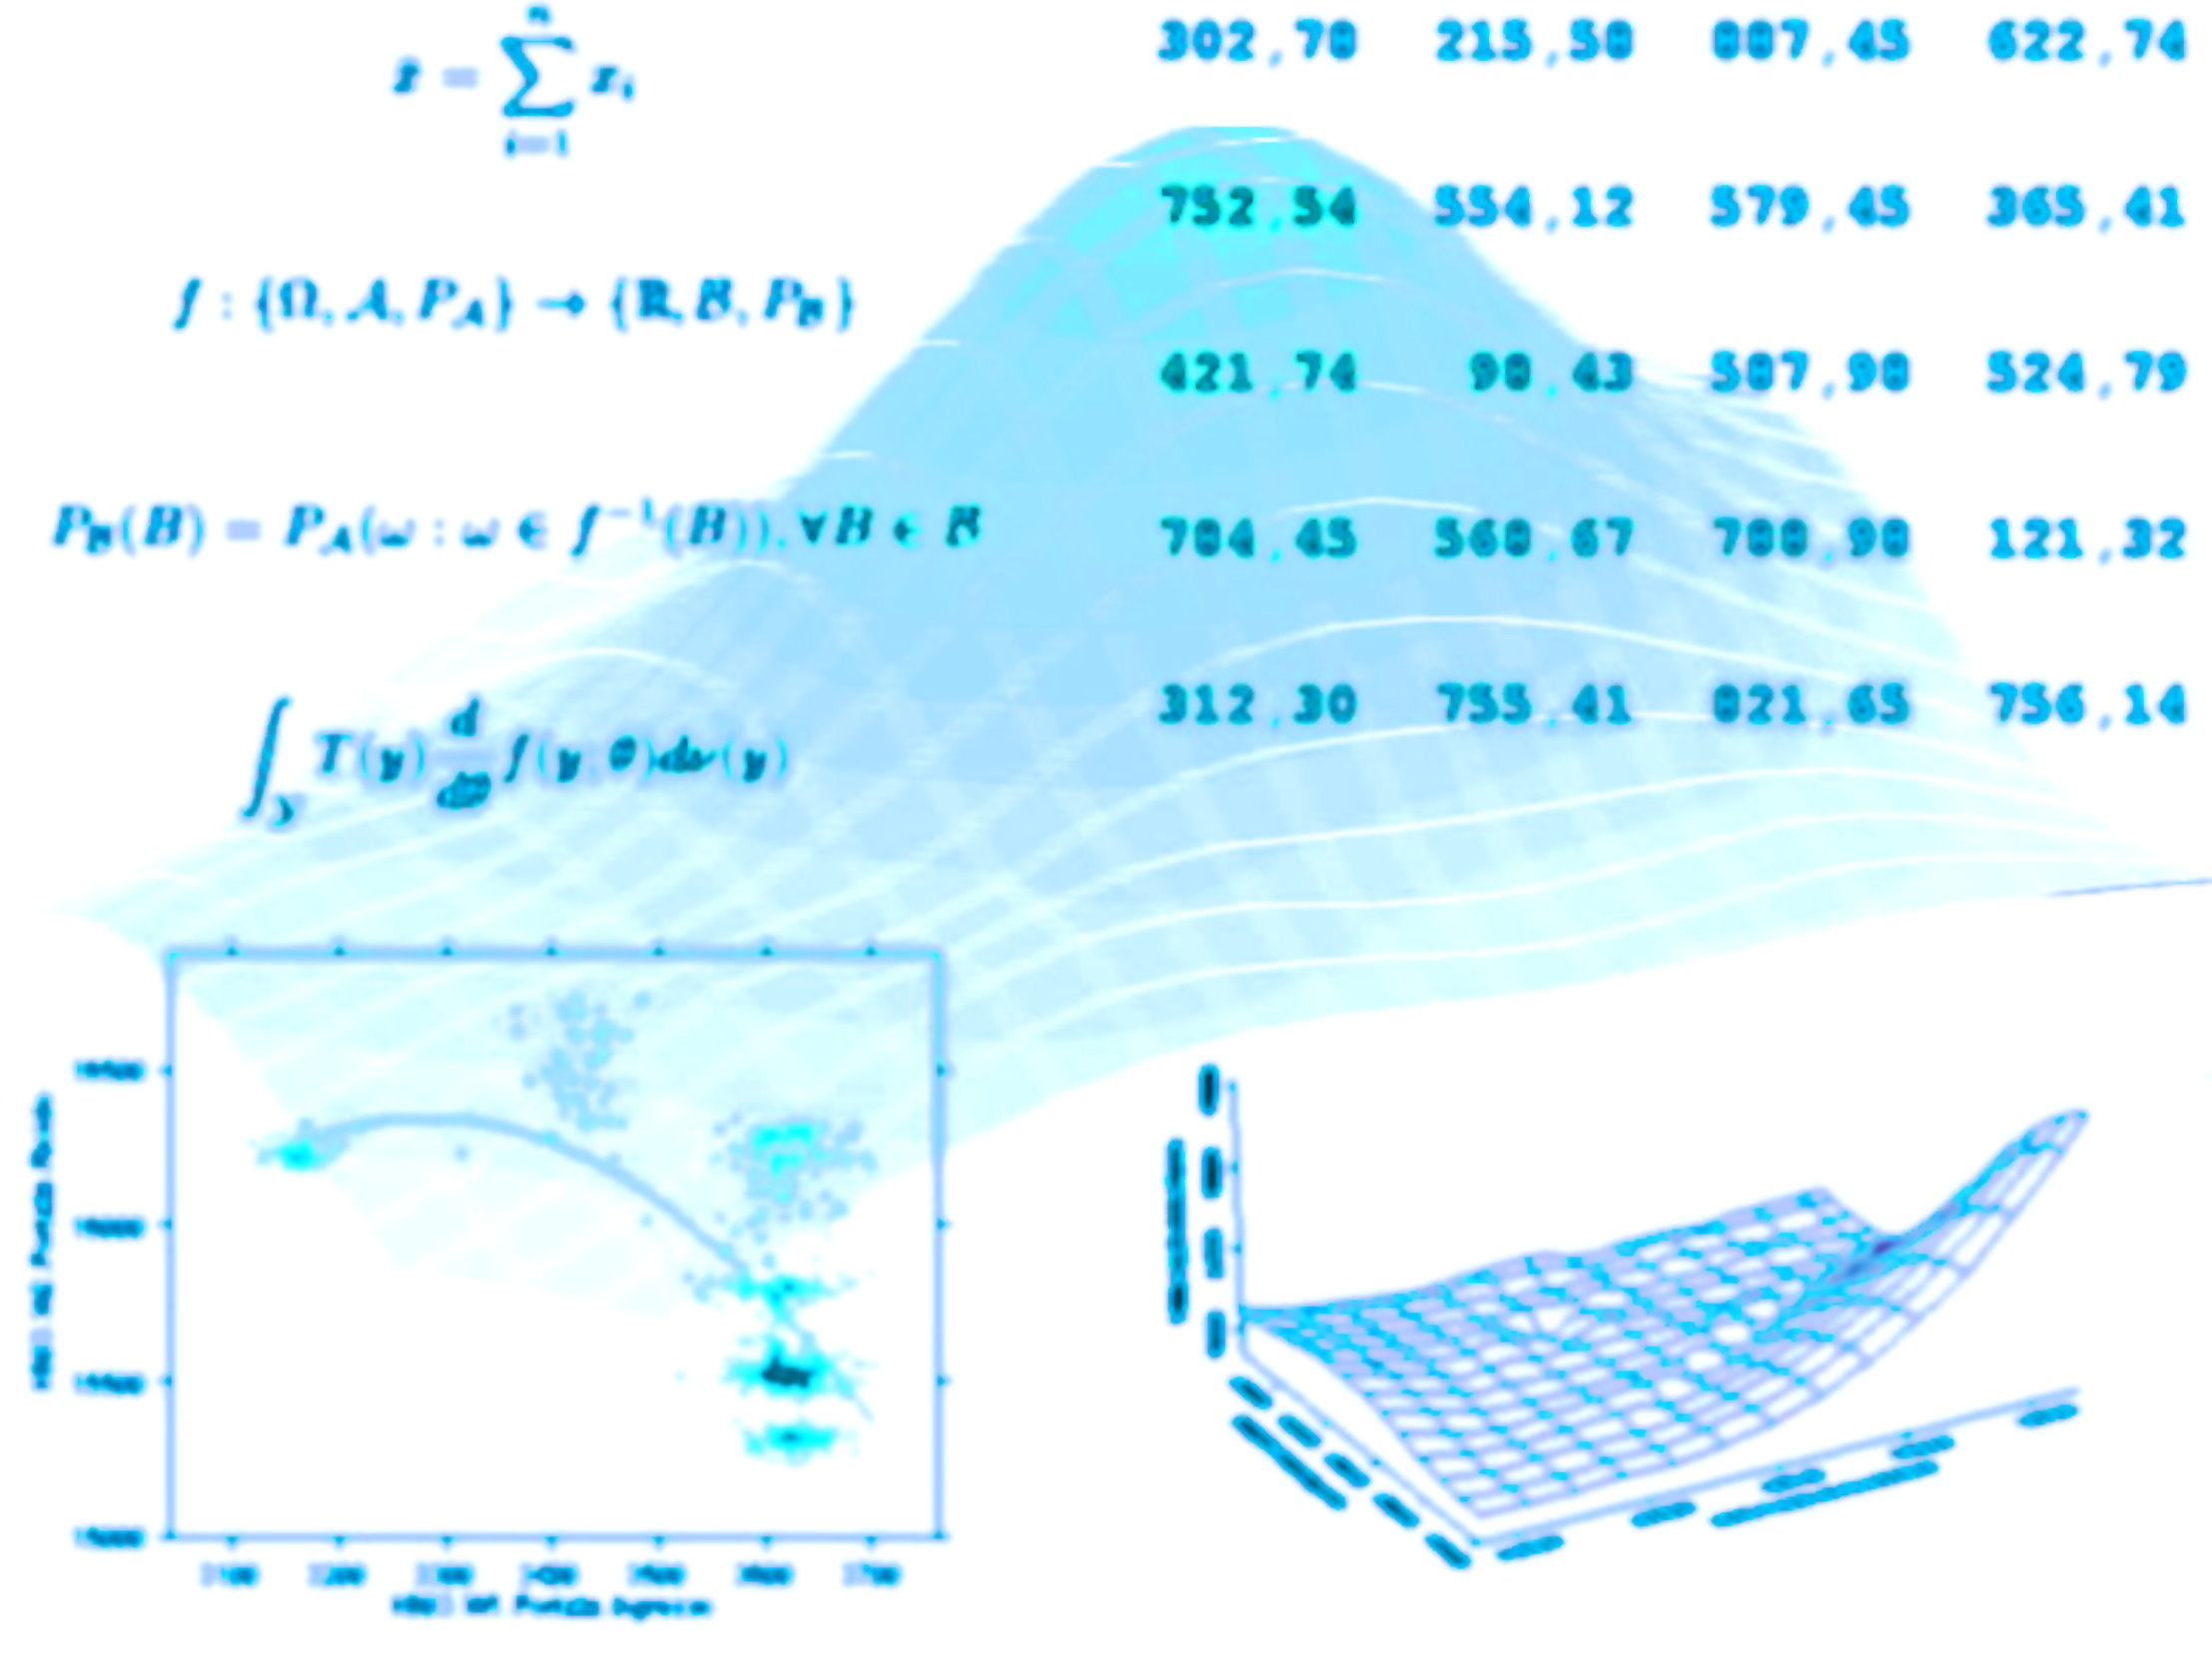
\includegraphics[width=.70\textwidth, height=11cm, keepaspectratio=false]{img/titolo2.png}
    \centering
  \end{figure}
\end{figtitolo}}



\definecolor{ablue}{rgb}{0.729, .824, .878}  % azzurro
\definecolor{iblue}{rgb}{0.0235294117647059,0.282352941176471,0.47843137254902}  % azzurro
\definecolor{ared}{rgb}{0.671,0.161,0.18}
% info box principale per prop e teoremi

\newtcolorbox{info}{
%beamer,
enhanced,
breakable,
colupper=iblue,
%frame style={upper left=blue,upper right=red,lower left=yellow,lower right=green},
colback=white!50!ablue,
%colframe=ablue,
%colframe=ablue!90!black,
width=\linewidth,
arc=0.1mm,
 boxsep=0mm,
 left=15mm,
left*=2mm,
%interior style={top color=iblue!10!white,middle color=iblue!20!white,bottom color=iblue!30!white},
interior style={top color=iblue!8!white,middle color=iblue!10!white,bottom color=iblue!12!white},
boxrule=0pt,
drop fuzzy shadow
}


\newtcolorbox{info2}{
enhanced,
colupper=iblue,
colback=white!50!ablue,
width=\linewidth,
arc=0.1mm,
 boxsep=0mm,
 left=15mm,
left*=2mm,
interior style={top color=iblue!8!white,middle color=iblue!10!white,bottom color=iblue!12!white},
boxrule=0pt,
drop fuzzy shadow
}

% info box con attenzione
\newenvironment{att}
  {
\begin{tcolorbox}[enhanced,arc=0.1mm,boxrule=1pt,colback=white,colframe=ared,title=\bf\small \fontfamily{lmss}\selectfont \faExclamationTriangle \hspace{.5 cm} Attenzione,drop fuzzy shadow]
}{
\end{tcolorbox}
  }
% info box con nota
\newenvironment{nota}
  {
\begin{tcolorbox}[enhanced,breakable,arc=0.1mm,boxrule=1pt,colback=white,colframe=iblue,title=\bf \fontfamily{lmss}\selectfont \faInfoCircle \hspace{.5 cm} Nota,drop fuzzy shadow]
}{
\end{tcolorbox}
  }

% per escludere le soluzioni togliere il commento a \excludecomment{sol} 
%
% \excludecomment{sol} 
% 
% e commentare da qui ↓

% info box con Soluzione

\newenvironment{sol}
  {
  \begin{tcolorbox}[enhanced,breakable,arc=0.1mm,boxrule=1pt,colback=white,colframe=iblue,
  title=\bf \fontfamily{lmss}\selectfont \hspace{.5 cm} Soluzione,drop fuzzy shadow]

}{
\end{tcolorbox}
  }

% a qui ↑ 

\newtcolorbox{titolo}{
enhanced,
beforeafter skip=0pt,
colupper=white,
colback=iblue,
width=\paperwidth,
arc=0.0mm,
boxsep=1mm,
%left=-2cm,
left*=-5cm,
boxrule=0pt,
grow to left by=3cm,
%grow to right by=3cm,
%enlarge right by=2cm
%drop fuzzy shadow
}

\newtcolorbox{figtitolo}{
enhanced,
beforeafter skip=0pt,
colupper=white,
colback=white,
width=\paperwidth,
arc=0.0mm,
boxsep=1mm,
%left=-2cm,
left*=-5cm,
boxrule=0pt,
%grow to left by=3cm,
%grow to right by=3cm,
%enlarge right by=2cm
%drop fuzzy shadow
}

\newenvironment{minip}
  {
\begin{tcolorbox}[enhanced, breakable,
left skip=1cm,
right skip=1cm,
%width=0.5\linewidth,
 % boxsep=5mm,
 % left=-15mm,
 % left*=20mm,
 arc=0mm,
boxrule=1pt,
colback=white,
drop fuzzy shadow]
}{
\end{tcolorbox}
  }

  
% definisco il comando mc che crea un cerchio intorno ad un carattere: di prossima soppresisone
\makeatletter
\newcommand\mc[1]{%
  \mathpalette\@mc{#1}%
}
\newcommand\@mc[2]{%
  \tikz[baseline=(math.base)] \node[draw,circle,inner sep=1pt] (math) {$\m@th#1#2$};%
}
\makeatother




% Roba vecchia


% qui di definisce quanti oggetti flottanti devono andare
% nella parte alta della pagine, nella bassa, ecc.
% meglio non toccare niente perché si fa un casino micidiale
% \renewcommand{\topfraction}{.35}
% \renewcommand{\bottomfraction}{.35}
% \renewcommand{\textfraction}{.50}
% \renewcommand{\floatpagefraction}{.99}
% \setcounter{topnumber}{1}
% \setcounter{bottomnumber}{2}
%\setcounter{totalnumber}{2}


% \newtheorem{thm}{Theorem}[section]
% \renewcommand{\thethm}{\arabic{section}.\textbf{\sffamily\arabic{thm}}}

% \newtcolorbox{info2}{
%   colback=black,
%   colframe=orange,
%   coltext=white,
%   boxsep=5pt,
%   arc=4pt}

%\definecolor{ablue}{rgb}{0.36, 0.54, 0.66} blue air

%\usepackage{tocloft}
%\usepackage{thmtools}

%\setlength{\fboxsep}{.4em}

% \newenvironment{info}{
%   \definecolor{shadecolor}{rgb}{0.729, .824, .878}  % azzurro
%   
% %  \definecolor{shadecolor}{rgb}{.9, .9, .9}  % grigio  
%   %\color{white}
%   \begin{shaded}}
%  {\end{shaded}}
 
% \newtcolorbox{nota}{
% colupper=black!75!blue,
% %frame style={upper left=blue,upper right=red,lower left=yellow,lower right=green},
% colback=white,
% colframe=red!75!black,
% %colframe=ablue!90!black,
% width=\linewidth,
% arc=0.5mm,
%  boxsep=0mm,
%  left=15mm,
% left*=2mm
% }

%\tcbuselibrary{all}
% \newtcolorbox{info2}{
% beamer,
% colback=yellow,
% colframe=orange,
% colupper=red,
% %colframe=ablue!90!black,
% width=\linewidth,
% arc=10mm,
%  boxsep=0mm,
%  left=15mm,
% left*=5.5mm
% }


\usepackage{booktabs}
\usepackage{longtable}
\usepackage{array}
\usepackage{multirow}
\usepackage{wrapfig}
\usepackage{float}
\usepackage{colortbl}
\usepackage{pdflscape}
\usepackage{tabu}
\usepackage{threeparttable}
\usepackage{threeparttablex}
\usepackage[normalem]{ulem}
\usepackage{makecell}
\usepackage{xcolor}
\ifLuaTeX
  \usepackage{selnolig}  % disable illegal ligatures
\fi
\usepackage[]{natbib}
\bibliographystyle{apalike}
\usepackage{bookmark}
\IfFileExists{xurl.sty}{\usepackage{xurl}}{} % add URL line breaks if available
\urlstyle{same}
\hypersetup{
  pdftitle={Eserciziario di Statistica},
  pdfauthor={Patrizio Frederic},
  hidelinks,
  pdfcreator={LaTeX via pandoc}}

\title{Eserciziario di Statistica}
\usepackage{etoolbox}
\makeatletter
\providecommand{\subtitle}[1]{% add subtitle to \maketitle
  \apptocmd{\@title}{\par {\large #1 \par}}{}{}
}
\makeatother
\subtitle{CLEAM AA 24/25}
\author{Patrizio Frederic}
\date{Aggiornato al 23-07-2025}

\begin{document}
\maketitle

{
\setcounter{tocdepth}{1}
\tableofcontents
}
\chapter*{Avvertenza}\label{avvertenza}
\addcontentsline{toc}{chapter}{Avvertenza}

\large

Questo lavoro è un work in progress, questa non è la versione definitiva, sconsiglio di stampare tutto.

\normalsize

Eserciziario di Statistica © 2024 di Patrizio Frederic è distribuito
sotto licenza CC BY-NC-ND 4.0
\url{https://creativecommons.org/licenses/by-nc-nd/4.0/}

You are free to:
Share --- copy and redistribute the material in any medium or format
The licensor cannot revoke these freedoms as long as you follow the license terms.
Under the following terms:
Attribution --- You must give appropriate credit, provide a link to the license, and indicate if changes were made. You may do so in any reasonable manner, but not in any way that suggests the licensor endorses you or your use.

NonCommercial --- You may not use the material for commercial purposes.

NoDerivatives --- If you remix, transform, or build upon the material, you may not distribute the modified material.

No additional restrictions --- You may not apply legal terms or technological measures that legally restrict others from doing anything the license permits.

\chapter*{Introduzione}\label{introduzione}
\addcontentsline{toc}{chapter}{Introduzione}

Qui si trovano le esercitazioni e i compiti passati del corso di Statistica
in formato html fruibili direttamente dal mio server.
Il pdf e il formato epub sono è scaricabili cliccando in alto.

Nel prossimo futuro, aggiungerò altri esercizi non presenti nei compiti solo a titolo
di esercitazione.

Patrizio Frederic

Bologna, il 23/07/2025.

\part{Esercizi per argomento}

\chapter{Esercizi di Statistica Descrittiva}\label{esercizi-di-statistica-descrittiva}

\section{Versione senza contesto}\label{versione-senza-contesto}

\subsection{Variante A}\label{variante-a}

Sono stati analizzati 2500 individui per investigare su fenomeno-x. É riportata qui di seguito la distribuzione in classi espressa in frequenza relativa.

\begin{tabular}{rrr}
\toprule
$[\text{x}_j,$ & $\text{x}_{j+1})$ & $f_j$\\
\midrule
0 & 3 & 0.2012\\
3 & 4 & 0.1764\\
4 & 5 & 0.1976\\
5 & 8 & 0.3236\\
8 & 20 & 0.1012\\
 &  & 1.0000\\
\bottomrule
\end{tabular}

\begin{enumerate}
\def\labelenumi{\alph{enumi}.}
\tightlist
\item
  Disegnare l'istogramma di densità percentuale.
\end{enumerate}

\begin{sol}

Ricordando che:

\begin{itemize}
\tightlist
\item
  \(n_j=f_j\cdot n\),
\item
  \(b_j=x_{j+1}-x_{j}\),
\item
  \(h_j=f_j/b_j\times 100\),
\end{itemize}

si consiglia di mettere i dati in tabella:

\begin{table}[H]
\centering
\begin{tabular}{rrrrrrr}
\toprule
$[\text{x}_j,$ & $\text{x}_{j+1})$ & $n_j$ & $f_j$ & $b_j$ & $h_j$ & $F_j$\\
\midrule
0 & 3 & 503 & 0.2012 & 3 & 6.7067 & 0.2012\\
3 & 4 & 441 & 0.1764 & 1 & 17.6400 & 0.3776\\
4 & 5 & 494 & 0.1976 & 1 & 19.7600 & 0.5752\\
5 & 8 & 809 & 0.3236 & 3 & 10.7867 & 0.8988\\
8 & 20 & 253 & 0.1012 & 12 & 0.8433 & 1.0000\\
 &  & 2500 & 1.0000 & 20 &  & \\
\bottomrule
\end{tabular}
\end{table}

\begin{center}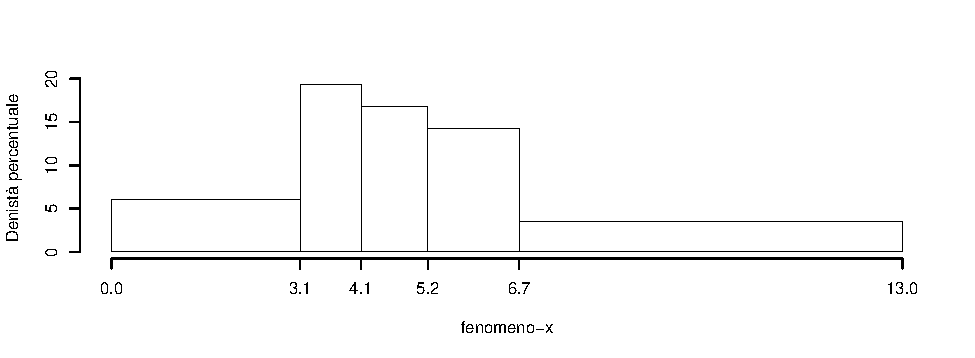
\includegraphics{Esami_passati_con_soluzioni_files/figure-latex/4-1} \end{center}

\end{sol}

\begin{enumerate}
\def\labelenumi{\alph{enumi}.}
\setcounter{enumi}{1}
\tightlist
\item
  calcolare il valore approssimato del percentile \(65\)-esimo, e tracciarlo nell'istogramma.
\end{enumerate}

\begin{sol}

\begin{eqnarray*}
  p &=&  0.65 , \text{essendo }F_{ 4 }= 0.8988  > 0.65  \Rightarrow j_{ 0.65 }= 4 \\
  x_{ 0.65 } &=& x_{\text{inf}; 4 } + \frac{ { 0.65 } - F_{ 3 }} {f_{ 4 }} \cdot b_{ 4 } \\
            &=&  5  + \frac {{ 0.65 } -  0.5752 } { 0.3236 } \cdot  3  \\
            &=&  5.693 
\end{eqnarray*}

\begin{center}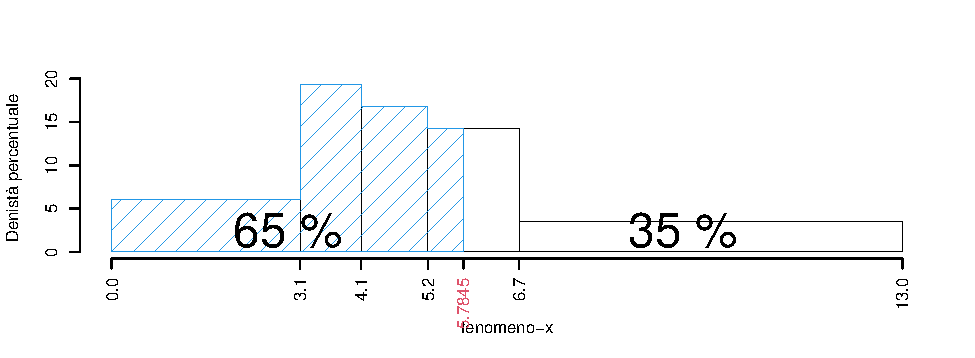
\includegraphics{Esami_passati_con_soluzioni_files/figure-latex/6-1} \end{center}

\end{sol}

\begin{enumerate}
\def\labelenumi{\alph{enumi}.}
\setcounter{enumi}{2}
\tightlist
\item
  Qual è il numero di individui con fenomeno-x superiore a 5?
\end{enumerate}

\begin{sol}
\begin{eqnarray*}
  \#(X>5) &=&  (f_4+f_5)\times n\\
            &=& (0.3236+0.1012)\times 2500\\
            &=& 1062,\text{ o alternativamente}\\
            &=& (1-F_3)\times n\\
            &=& (1-0.5752)\times 2500\\
            &=& 1062
\end{eqnarray*}
\begin{eqnarray*}
     \%(X> 5.2 ) &=& ( 8 - 5.2 )\times h_{ 4 }+ f_{ 5 }\times 100 \\
              &=& ( 2.8 )\times 10.79 + ( 0.1012 )\times 100 \\
              &=&  0.4032 \times(100)\\
     \#(X> 5.2 ) &\approx& 1008 
         \end{eqnarray*}

\end{sol}

\begin{enumerate}
\def\labelenumi{\alph{enumi}.}
\setcounter{enumi}{3}
\tightlist
\item
  Analizzare la relazione tra media, mediana e moda alla luce del istogramma di densità.
\end{enumerate}

\begin{sol}
È presente un'evidente asimmetria positiva (coda lunga a dx) e quindi

\[Moda>x_{0.5}>\bar x\]

\end{sol}

\subsection{Variante B}\label{variante-b}

Sono stati analizzati 250 individui per investigare su dati-x. È riportata qui di seguito la distribuzione in classi espressa in frequenza assoluta.

\begin{table}[H]
\centering
\begin{tabular}{rrr}
\toprule
$[\text{x}_j,$ & $\text{x}_{j+1})$ & $n_j$\\
\midrule
0 & 7 & 73\\
7 & 8 & 29\\
8 & 9 & 65\\
9 & 10 & 83\\
 &  & 250\\
\bottomrule
\end{tabular}
\end{table}

\begin{enumerate}
\def\labelenumi{\alph{enumi}.}
\tightlist
\item
  Disegnare l'istogramma di densità percentuale.
\end{enumerate}

\begin{sol}

Ricordando che:

\begin{itemize}
\tightlist
\item
  \(f_j=n_j/n\),
\item
  \(b_j=x_{j+1}-x_{j}\),
\item
  \(h_j=f_j/b_j\times 100\),
\end{itemize}

si consiglia di mettere i dati in tabella:

\begin{table}[H]
\centering
\begin{tabular}{rrrrrrr}
\toprule
$[\text{x}_j,$ & $\text{x}_{j+1})$ & $n_j$ & $f_j$ & $b_j$ & $h_j$ & $F_j$\\
\midrule
0 & 7 & 73 & 0.292 & 7 & 4.171 & 0.292\\
7 & 8 & 29 & 0.116 & 1 & 11.600 & 0.408\\
8 & 9 & 65 & 0.260 & 1 & 26.000 & 0.668\\
9 & 10 & 83 & 0.332 & 1 & 33.200 & 1.000\\
 &  & 250 & 1.000 & 10 &  & \\
\bottomrule
\end{tabular}
\end{table}

\end{sol}

\begin{enumerate}
\def\labelenumi{\alph{enumi}.}
\setcounter{enumi}{1}
\tightlist
\item
  calcolare il valore approssimato del percentile \(25\)-esimo, e tracciarlo nell'istogramma.
\end{enumerate}

\begin{sol}

\begin{eqnarray*}
  p &=&  0.25 , \text{essendo }F_{ 1 }= 0.292  > 0.25  \Rightarrow j_{ 0.25 }= 1 \\
  x_{ 0.25 } &=& x_{\text{inf}; 1 } + \frac{ { 0.25 } - F_{ 0 }} {f_{ 1 }} \cdot b_{ 1 } \\
            &=&  0  + \frac {{ 0.25 } -  0 } { 0.292 } \cdot  7  \\
            &=&  5.993 
\end{eqnarray*}

\begin{center}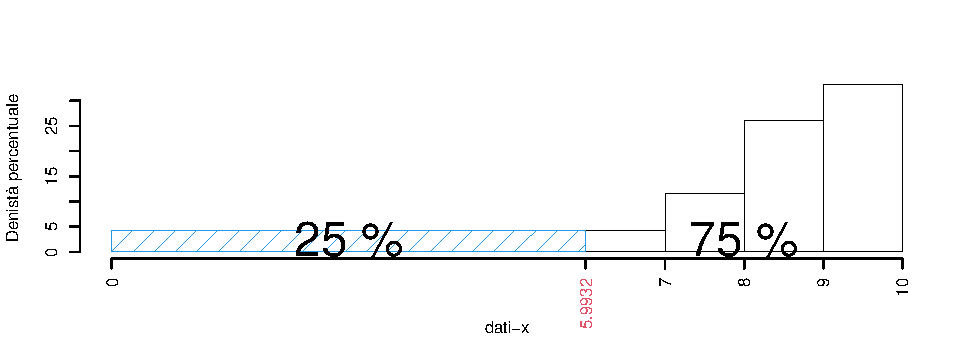
\includegraphics{Esami_passati_con_soluzioni_files/figure-latex/01-descr-8-1} \end{center}

\end{sol}

\begin{enumerate}
\def\labelenumi{\alph{enumi}.}
\setcounter{enumi}{2}
\tightlist
\item
  Calcolare il numero di individui maggiori del 75-esimo percentile, \(x_{0.75}\)
\end{enumerate}

\begin{sol}
Per definizione
\[
\%(X\le x_{0.75})=75\%
\]
e quindi
\[
\%(X> x_{0.75}) = 25%
\]
calcoliamo il 25\% di \(n=250\) e otteniamo
\[
\#(X>x_{0.75})=250\times 0.25=62.5
\]

\end{sol}

\begin{enumerate}
\def\labelenumi{\alph{enumi}.}
\setcounter{enumi}{3}
\tightlist
\item
  calcolare il valore approssimato della media aritmetica \(\bar x\) e della varianza \(\sigma^2\).
\end{enumerate}

\begin{sol}

Calcoliamo i valori medi delle classi \(\bar x_j\), il loro quadrato \(\bar x_j^2\) e li pesiamo con gli \(n_j\)

\begin{table}[H]
\centering
\begin{tabular}{rrrrrr}
\toprule
$[\text{x}_j,$ & $\text{x}_{j+1})$ & $n_j$ & $f_j$ & $\bar{\text{x}}_j$ & $\bar{\text{x}}_j^2$\\
\midrule
0 & 7 & 73 & 0.292 & 3.5 & 12.25\\
7 & 8 & 29 & 0.116 & 7.5 & 56.25\\
8 & 9 & 65 & 0.260 & 8.5 & 72.25\\
9 & 10 & 83 & 0.332 & 9.5 & 90.25\\
 &  & 250 & 1.000 &  & \\
\bottomrule
\end{tabular}
\end{table}

e quindi
\[
\bar x= \frac 1n\sum_{j=1}^k\bar x_jn_j=\frac{1814}{250}=7.256
\]

e quindi
\[
\sigma^2= \frac 1n\sum_{j=1}^k\bar x_j^2n_j-\bar x^2=\frac{14712.5}{250}-(7.256)^2=6.2005
\]

\end{sol}

\subsection{Variante C}\label{variante-c}

Sono stati analizzati 200 individui per investigare su dati-x. Sono noti i percentili
\(x_{0.21}=11\), \(x_{0.42}=23\), \(x_{0.6}=39\), \(x_{0.78}=62\), il minimo è 0, il massimo è 150.

\begin{enumerate}
\def\labelenumi{\alph{enumi}.}
\tightlist
\item
  Disegnare l'istogramma di densità percentuale.
\end{enumerate}

\begin{sol}

Ricordando che:

\begin{itemize}
\tightlist
\item
  \(f_1=F_1\), \(f_2=F_2-F_1\),\ldots,\(f_j = F_j-F_{j-1}\),
\item
  \(b_j=x_{j+1}-x_{j}\),
\item
  \(h_j=f_j/b_j\times 100\),
\end{itemize}

si consiglia di mettere i dati in tabella:

\begin{table}[H]
\centering
\begin{tabular}{rrrrrr}
\toprule
$[\text{x}_j,$ & $\text{x}_{j+1})$ & $f_j$ & $b_j$ & $h_j$ & $F_j$\\
\midrule
0 & 11 & 0.210 & 11 & 1.9091 & 0.21\\
11 & 23 & 0.210 & 12 & 1.7500 & 0.42\\
23 & 39 & 0.185 & 16 & 1.1562 & 0.60\\
39 & 62 & 0.175 & 23 & 0.7609 & 0.78\\
62 & 150 & 0.220 & 88 & 0.2500 & 1.00\\
 &  & 1.000 & 150 &  & \\
\bottomrule
\end{tabular}
\end{table}

e infine disegnare il grafico

\begin{center}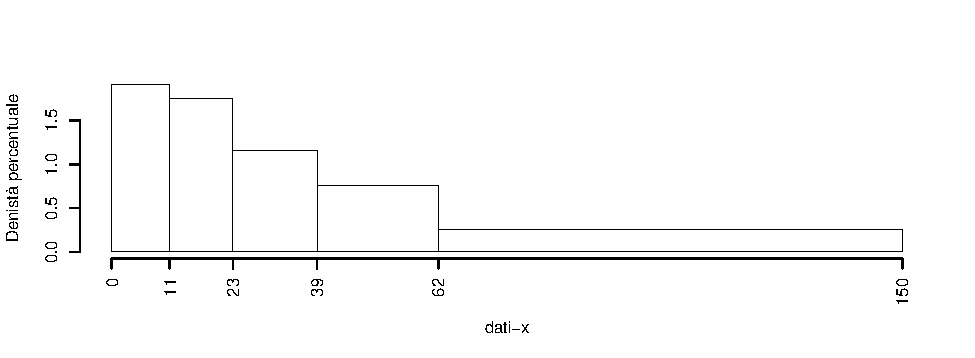
\includegraphics{Esami_passati_con_soluzioni_files/figure-latex/01-descr-10-1} \end{center}

\end{sol}

\begin{enumerate}
\def\labelenumi{\alph{enumi}.}
\setcounter{enumi}{1}
\tightlist
\item
  Calcolare le frequenze assolute
\end{enumerate}

\begin{sol}

Ricordando che:
\[
n_j=f_j\times n
\]

e mettendo in tabella, otteniamo

\begin{table}[H]
\centering
\begin{tabular}{rrrr}
\toprule
$[\text{x}_j,$ & $\text{x}_{j+1})$ & $f_j$ & $n_j$\\
\midrule
0 & 11 & 0.210 & 42\\
11 & 23 & 0.210 & 42\\
23 & 39 & 0.185 & 37\\
39 & 62 & 0.175 & 35\\
62 & 150 & 0.220 & 44\\
 &  & 1.000 & 200\\
\bottomrule
\end{tabular}
\end{table}

\end{sol}

\begin{enumerate}
\def\labelenumi{\alph{enumi}.}
\setcounter{enumi}{2}
\tightlist
\item
  Calcolare la percentuale approssimata di individui con dati-x inferiore a 45
\end{enumerate}

\begin{sol}

\begin{eqnarray*}
\%(X<45)   &\approx&  \%(X<39)+(45-39)\times h_4\\
&=& F_3\times 100+(45-39)\times 0.7609\\
&=& 0.605\times 100 + 6\times 0.7609\\
&=& 65.0652\%
\end{eqnarray*}

graficamente

\begin{center}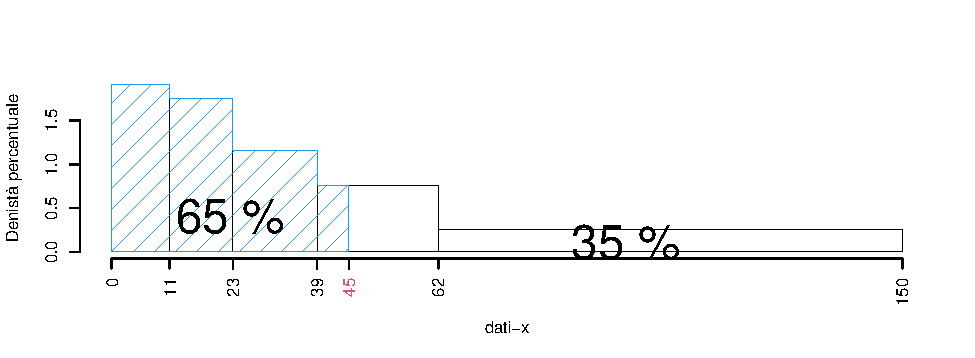
\includegraphics{Esami_passati_con_soluzioni_files/figure-latex/01-descr-12-1} \end{center}

\end{sol}

\begin{enumerate}
\def\labelenumi{\alph{enumi}.}
\setcounter{enumi}{3}
\tightlist
\item
  Calcolare la percentuale approssimata di individui con dati-x compresa tra 45 e il 90-esimo percentile, \(x_{0.90}\).
\end{enumerate}

\begin{sol}

Per calcolare
\[
\%(45< X < x_{0.90})
\]
non c'è bisogno di calcolare \(x_{0.90}\), infatti dal punto precedente sappiamo che

\begin{eqnarray*}
\%(X<45)   &\approx&  \%(X<39)+(45-39)\times h_4\\
&=& F_3+(45-39)\times 0.7609\\
&=& 0.605\times 100 + 6\times 0.7609\\
&=& 65.0652\%
\end{eqnarray*}
dalla teoria sappiamo che
\[
\%(X<x_{0.90})=90\%
\]
e quindi
\begin{eqnarray*}
\%(45< X < x_{0.90}) &=& 90\%-65.0652\%\\
                     &=& 24.9348\%
\end{eqnarray*}

graficamente

\begin{center}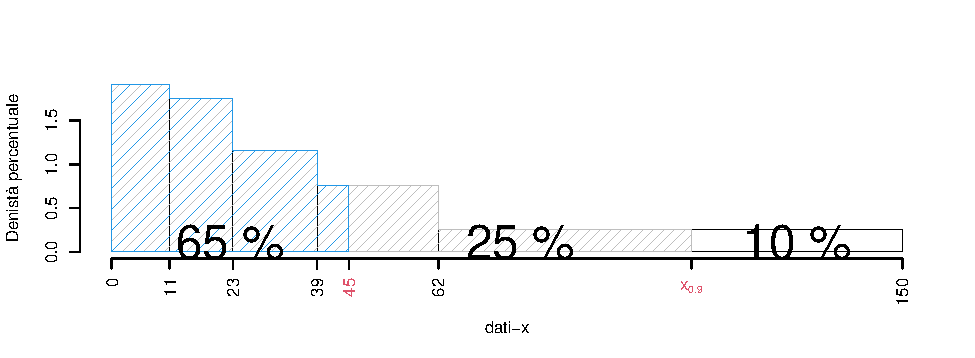
\includegraphics{Esami_passati_con_soluzioni_files/figure-latex/01-descr-13-1} \end{center}

\end{sol}

\section{Varianti con contesto (eserciziario)}\label{varianti-con-contesto-eserciziario}

\subsection{Esercizio: Conteggi}\label{esercizio-conteggi}

La figura seguente riporta l'istogramma relativo a un campione
di 200 imprese classificate sulla base del numero di addetti
secondo le classi: \(0-9\) addetti, \(10-19\) addetti, \(20-49\) addetti,
\(50-99\) addetti, \(100-249\) addetti.
Si noti che sull'asse delle ordinate è riportata la densità
percentuale.

\emph{Si noti che, a causa dell'ampiezza della scala dei valori, i dettagli dell'istogramma \textbf{non si leggono} sul grafico e, pertanto, non sono stati riportati gli estremi delle classi sull'asse delle ascisse, \(X\), e i dati si evincono dal testo}

\begin{center}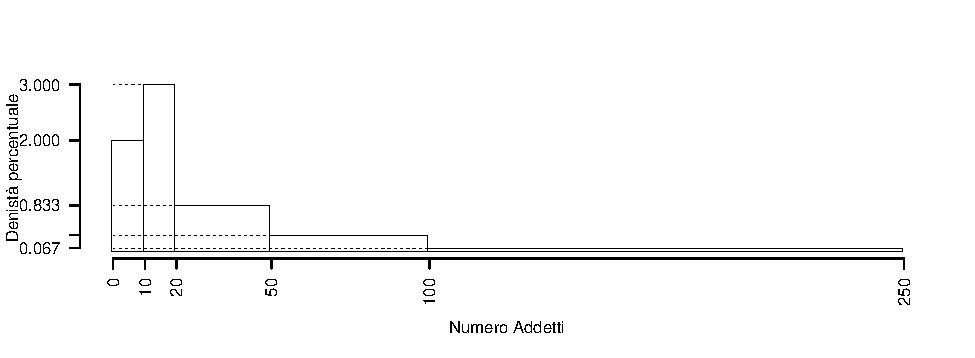
\includegraphics{Esami_passati_con_soluzioni_files/figure-latex/01-descr-15-1} \end{center}

\begin{sol}
Il testo fornisce una rappresentazione grafica.
Per rispondere alle domande successive occorre partire dalla
rappresentazione in una tabella di frequenze (relative o, come
conviene in questo caso, percentuali).
Si devono determinare, quindi, le aree dei rettangoli per ottenere
le percentuali di unità statistiche contenute nelle varie classi.
Si procede come segue:

\begin{longtable}[]{@{}
  >{\raggedright\arraybackslash}p{(\columnwidth - 6\tabcolsep) * \real{0.2361}}
  >{\raggedright\arraybackslash}p{(\columnwidth - 6\tabcolsep) * \real{0.2639}}
  >{\raggedright\arraybackslash}p{(\columnwidth - 6\tabcolsep) * \real{0.2222}}
  >{\raggedright\arraybackslash}p{(\columnwidth - 6\tabcolsep) * \real{0.2778}}@{}}
\toprule\noalign{}
\begin{minipage}[b]{\linewidth}\raggedright
Area Classi disgiunte
\end{minipage} & \begin{minipage}[b]{\linewidth}\raggedright
Ampiezza Classi congiunte
\end{minipage} & \begin{minipage}[b]{\linewidth}\raggedright
\(\times\)densità
\end{minipage} & \begin{minipage}[b]{\linewidth}\raggedright
frequenze perc.
\end{minipage} \\
\midrule\noalign{}
\endhead
\bottomrule\noalign{}
\endlastfoot
\(A(  0- 9)\) & \(=[  9,5 -(-0,5)]\) & \(\times 2\) & \(= 20\%\) \\
\(A( 10- 19)\) & \(=[ 19,5 -  9,5)]\) & \(\times 3\) & \(= 30\%\) \\
\(A( 20- 49)\) & \(=[ 49,5 - 19,5)]\) & \(\times 0.833\) & \(= 25\%\) \\
\(A( 50- 99)\) & \(=[ 99,5 - 49,5)]\) & \(\times 0.3\) & \(= 15\%\) \\
\(A(100-249)\) & \(=[249,5 - 99,5)]\) & \(\times 0.066\) & \(= 10\%\) \\
\end{longtable}

A questo punto è possibile costruire la tabella della
distribuzione delle frequenze percentuali della \(X\), numero
di addetti delle imprese.

\begin{table}[H]
\centering
\begin{tabular}{rrrrrrr}
\toprule
$[\text{x}_j,$ & $\text{x}_{j+1})$ & $n_j$ & $f_j$ & $b_j$ & $h_j$ & $F_j$\\
\midrule
-0.5 & 9.5 & 40 & 0.20 & 10 & 2.0000 & 0.20\\
9.5 & 19.5 & 60 & 0.30 & 10 & 3.0000 & 0.50\\
19.5 & 49.5 & 50 & 0.25 & 30 & 0.8333 & 0.75\\
49.5 & 99.5 & 30 & 0.15 & 50 & 0.3000 & 0.90\\
99.5 & 249.5 & 20 & 0.10 & 150 & 0.0667 & 1.00\\
\bottomrule
\end{tabular}
\end{table}

La funzione di ripartizione è utile quando si devono determinare
la mediana (o la classe che la contiene) e/o la classe che contiene
un determinato percentile.
Un'altra definizione di percentile, infatti, utilizza la
funzione cumulata delle frequenze percentuali, \(F_{\%; j}\).
Il percentile \(p\)-esimo è il ``primo'' valore della \(x\),
indicato con \(x_{p}\), nel quale la \(F_{\%; j}(x_{p})\) è uguale
o supera il \((100 \times p)\)\%.

\end{sol}

\begin{enumerate}
\def\labelenumi{\alph{enumi}.}
\tightlist
\item
  Qual è l'intervallo con il maggior numero di imprese?
\end{enumerate}

\begin{sol}
L'intervallo \([10;\ 19]\).

\end{sol}

\begin{enumerate}
\def\labelenumi{\alph{enumi}.}
\setcounter{enumi}{1}
\tightlist
\item
  Qual è il numero di imprese che hanno addetti
  nella classe \([0,\, 9]\)?
\end{enumerate}

\begin{sol}
\(f\left( 0 \vdash 10 \right) = \frac{10 \,\times\, 2} {100}\ 200 = 40\) (circa).

\end{sol}

\begin{enumerate}
\def\labelenumi{\alph{enumi}.}
\setcounter{enumi}{2}
\tightlist
\item
  In quale classe si trova il 15\(^{o}\) percentile?
\end{enumerate}

\begin{sol}
Il 15\(^{o}\) percentile si trova nella classe \([0;\, 9]\).

\end{sol}

\begin{enumerate}
\def\labelenumi{\alph{enumi}.}
\setcounter{enumi}{3}
\tightlist
\item
  Qual è l'intervallo che contiene la mediana?
\end{enumerate}

\begin{sol}
Il 50\% delle imprese è contenuto esattamente nelle prime due classi.
La mediana si trova dunque tra la fine dell'intervallo
\([10;\, 19]\) e l'inizio dell'intervallo \([20;\, 49]\).
Si potrebbe, quindi, dire che la mediana è 20?
No, perché non è noto come sono distribuite le imprese nella classe
\([20;\, 49]\); infatti, ipoteticamente, tutte le imprese della classe
potrebbero avere 49 addetti e, in tal caso la mediana sarebbe 49 o
la media tra 49 e 19.

\end{sol}

\begin{enumerate}
\def\labelenumi{\alph{enumi}.}
\setcounter{enumi}{4}
\tightlist
\item
  In quale classe si trova il 75\(^{o}\) percentile?
\end{enumerate}

\begin{sol}
Il 75\(^{o}\) percentile si trova nella classe \([50;\, 99]\).

NB: il 75\% della frequenza cumulata si trova proprio nella terza
classe \([20;\, 49]\); perciò un valore successivo potrebbe essere
il 75\(^{o}\) percentile, per esempio 50.
Non si sa, come già detto per la mediana, se tra i dati vi sia
una impresa con 50 addetti e, dunque, si può solo dire che la
classe contenente il 75\(^{o}\) percentile è la successiva.

\end{sol}

\begin{enumerate}
\def\labelenumi{\alph{enumi}.}
\setcounter{enumi}{5}
\tightlist
\item
  Quale relazione ci si deve attendere
  fra media e mediana per i dati proposti?
\end{enumerate}

\begin{sol}
L'esame del grafico mostra che vi è una asimmetria a destra
(o positiva); pertanto, risulta (media\(>\)mediana); infatti, in
base ai dati dell'istogramma, eseguendo i calcoli si trova che
\(\bar{x}=43\) e \(x_{0,5}=20\).

\end{sol}

\begin{enumerate}
\def\labelenumi{\alph{enumi}.}
\setcounter{enumi}{6}
\tightlist
\item
  Determinare il valore approssimato della mediana,
  assumendo la distribuzione uniforme dei casi contenuti nella classe
  che contiene la mediana.
\end{enumerate}

\begin{sol}
\begin{eqnarray*}
  p &=&  0.5 , \text{essendo }F_{ 2 }= 0.5  > 0.5  \Rightarrow j_{ 0.5 }= 2 \\
  x_{ 0.5 } &=& x_{\text{inf}; 2 } + \frac{ { 0.5 } - F_{ 1 }} {f_{ 2 }} \cdot b_{ 2 } \\
            &=&  9.5  + \frac {{ 0.5 } -  0.2 } { 0.3 } \cdot  10  \\
            &=&  19.5 
\end{eqnarray*}

\end{sol}

\begin{enumerate}
\def\labelenumi{\alph{enumi}.}
\setcounter{enumi}{7}
\tightlist
\item
  Definizione formale di percentile.
\end{enumerate}

\begin{sol}
Il \(p\)-esimo percentile (\(0 \le p\le 1\)) del carattere \(X\)
è quel valore di \(X\), indicato con \(x_{p}\), tale che

\begin{eqnarray*}
p       &=& F(x_{p}) \\
p       &=& A(X < x_{p})      \qquad \mbox{Area\ totale\ uguale\ 1} \\
p \times 100 &=& \%(X < x_{p}) \qquad \mbox{Area\ totale\ uguale\ 100} 
\end{eqnarray*}

\end{sol}

\subsection{Esercizio Dati Continui}\label{esercizio-dati-continui}

L'istogramma seguente mostra la distribuzione per
classi di cilindrata delle autovetture iscritte al Pubblico
Registro Automobilistico (dati aggiornati al 31/12/99;
fonte www.aci.it).
Il numero di autovetture censite è pari a 32027945; ma,
per comodità nei calcoli, il numero totale, \(n\), è stato
posto pari a 3000.
Sopra ogni rettangolo è indicato il valore delle
densità di frequenza percentuale.

\begin{center}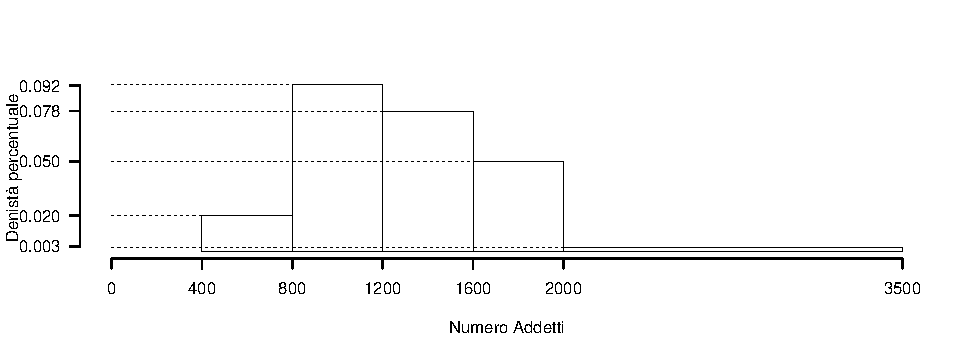
\includegraphics{Esami_passati_con_soluzioni_files/figure-latex/01-descr-18-1} \end{center}

\begin{enumerate}
\def\labelenumi{\alph{enumi}.}
\tightlist
\item
  Qual è la percentuale di autovetture comprese nella seconda classe?
\end{enumerate}

\begin{sol}
La seconda classe ha ampiezza pari a \(1200 - 800 = 400\).
La densità percentuale è pari a 0.0925 e, quindi, la
percentuale di autoveicoli con cilindrata compresa in tale
intervallo è \(0.0925 \times 400 = 37\%\).

\end{sol}

\begin{enumerate}
\def\labelenumi{\alph{enumi}.}
\setcounter{enumi}{1}
\tightlist
\item
  In quale classe cade la mediana?
\end{enumerate}

\begin{sol}
La percentuale di autoveicoli nella prima classe è
\(0.02 \,\times\, 400 = 8\%\).
La percentuale di autoveicoli nella seconda classe è \(37\%\).
La percentuale di autoveicoli nella terza classe è
\(0.0775 \,\times\, 400 = 31\%\).
Dal momento che \(8\% +37\% < 50\%\), mentre
\(8\% +37\% +31\% > 50\%\), la mediana appartiene
alla terza classe, ovvero è compresa fra 1200cc e 1600cc.

\end{sol}

\begin{enumerate}
\def\labelenumi{\alph{enumi}.}
\setcounter{enumi}{2}
\tightlist
\item
  Determinare il valore approssimato della mediana,
  assumendo la distribuzione uniforme dei casi contenuti
  nella classe che contiene la mediana.
\end{enumerate}

\begin{sol}
Sia \(m\) il numero della classe contenente la mediana:

\begin{eqnarray*}
  p &=&  0.5 , \text{essendo }F_{ 3 }= 0.76  > 0.5  \Rightarrow j_{ 0.5 }= 3 \\
  x_{ 0.5 } &=& x_{\text{inf}; 3 } + \frac{ { 0.5 } - F_{ 2 }} {f_{ 3 }} \cdot b_{ 3 } \\
            &=&  1200  + \frac {{ 0.5 } -  0.45 } { 0.31 } \cdot  400  \\
            &=&  1265 
\end{eqnarray*}

\end{sol}

\begin{enumerate}
\def\labelenumi{\alph{enumi}.}
\setcounter{enumi}{3}
\tightlist
\item
  Qual è la ``classe modale'' ?
\end{enumerate}

\begin{sol}
La ``classe modale'' è quella con la massima densità di frequenza
(il rettangolo con l'altezza maggiore) e corrisponde alla classe
800--1200 con una percentuale (seconda classe) pari a \(37\%\).
In questo caso è anche la classe con la percentuale di più
alta; infatti, la percentuale di autoveicoli nella terza classe
è \(0.0775 \,\times\, 400 = 31\%\).
Le altre classi hanno una percentuale inferiore, come si può
osservare considerando le unità di misura del grafico e i
relativi valori.

\end{sol}

\begin{enumerate}
\def\labelenumi{\alph{enumi}.}
\setcounter{enumi}{4}
\tightlist
\item
  Giulio ha una macchina con cilindrata pari a 625cc. Indicare la risposta corretta:
\end{enumerate}

\begin{itemize}
\tightlist
\item
  \(\Box \;\) l'auto di Giulio è molto potente, infatti meno del 9\% delle auto ha cilindrata inferiore
\item
  \(\Box \;\) l'auto di Giulio è molto potente, infatti più del 90\% delle auto ha cilindrata inferiore
\item
  \(\Box \;\) l'auto di Giulio è poco potente, infatti meno del 9\% delle auto ha cilindrata inferiore
\item
  \(\Box \;\) l'auto di Giulio è poco potente, infatti più del 9\% delle auto ha cilindrata inferiore
\end{itemize}

\begin{sol}
l'auto di Giulio è poco potente, infatti meno del 9\% delle auto ha cilindrata inferiore

\end{sol}

\subsection{Esercizio (variante 1)}\label{esercizio-variante-1}

La distribuzione delle frequenze assolute della cilindrata
delle autovetture iscritte al Pubblico Registro Automobilistico
(dati aggiornati al 31/12/99; fonte www.aci.it) è riportata
nella tabella seguente.
Il numero di autovetture censite, per comodità è stato posto
pari a 3000 (decine di migliaia, si veda l'esercizio precedente).

\begin{tabular}{rrr}
\toprule
$[\text{x}_j,$ & $\text{x}_{j+1})$ & $n_j$\\
\midrule
400 & 800 & 240\\
800 & 1200 & 1110\\
1200 & 1600 & 930\\
1600 & 2000 & 600\\
2000 & 3500 & 120\\
\bottomrule
\end{tabular}

\begin{enumerate}
\def\labelenumi{\alph{enumi}.}
\tightlist
\item
  Qual è la percentuale di autovetture comprese nella seconda classe?
\end{enumerate}

\begin{sol}
\(f_{\%;\, 2} = 100 \,\times\, 1110/3000 = 37\%\).

\end{sol}

\begin{enumerate}
\def\labelenumi{\alph{enumi}.}
\setcounter{enumi}{1}
\tightlist
\item
  In quale classe cade la mediana?
\end{enumerate}

\begin{sol}
Per individuare la classe che contiene la mediana,
si cumulano le percentuali a partire dalla prima
classe e ci si arresta appena si supera il 50\%.
Per completezza e comodità si riporta la seguente
tabella che contiene le frequenze percentuali e le
frequenze percentuali cumulate, \(F_{\%;\, j}\).

\begin{tabular}{rrrrr}
\toprule
$[\text{x}_j,$ & $\text{x}_{j+1})$ & $n_j$ & $f_j$ & $F_j$\\
\midrule
400 & 800 & 240 & 0.08 & 0.08\\
800 & 1200 & 1110 & 0.37 & 0.45\\
1200 & 1600 & 930 & 0.31 & 0.76\\
1600 & 2000 & 600 & 0.20 & 0.96\\
2000 & 3500 & 120 & 0.04 & 1.00\\
\bottomrule
\end{tabular}

La classe che contiene la mediana è 120-160 perché in questa
la frequenza percentuale cumulata ha superato il 50\%.

Si noti che un modo diverso di fornire i dati è riportare
nel grafico: le densità percentuali, \(h_{\%;\, j}\), oppure
le densità di frequenza relativa, \(h_{j}\); si ricordi che:

\begin{displaymath}
h_{j}       = \frac{f_{j}}  {x_{j+1} - x_{j}},  \qquad\qquad
h_{\%;\, j} = 100\ \frac{f_{j}}  {x_{j+1} - x_{j}}
            = \frac{f_{\%;\, j}} {x_{j+1} - x_{j}}\, .
\end{displaymath}

Si noti che in casi come questi, in cui si riportano le
frequenze assolute, \(n_{j}\), occorre esaminare con attenzione
la leggenda dell'asse delle ordinate perché può capitare
che le \(n_{j}\) si riportino direttamente sull'asse delle
ordinate.

\end{sol}

\subsection{Esercizio (variante 2)}\label{esercizio-variante-2}

La distribuzione delle frequenze relative della cilindrata
delle autovetture iscritte al Pubblico Registro Automobilistico
(dati aggiornati al 31/12/99; fonte www.aci.it) è riportata
nella tabella seguente.
Il numero di autovetture censite è pari a 320.27 centinaia
di migliaia (\(10^{5}\)).

\begin{tabular}{rrr}
\toprule
$[\text{x}_j,$ & $\text{x}_{j+1})$ & $f_j$\\
\midrule
400 & 800 & 0.08\\
800 & 1200 & 0.37\\
1200 & 1600 & 0.31\\
1600 & 2000 & 0.20\\
2000 & 3500 & 0.04\\
\bottomrule
\end{tabular}

\begin{enumerate}
\def\labelenumi{\alph{enumi}.}
\tightlist
\item
  Disegnare l'istogramma (delle densità relative) della
  distribuzione della cilindrata delle auto in circolazione.
\end{enumerate}

\begin{sol}
Per disegnare l'istogramma occorrono le altezze, \(h_{i}\),
dei rettangoli da disegnare per ogni classe: i calcoli sono
riportati di séguito:

\begin{eqnarray*}
h_{j} &=& \frac{f_{j}} {b_{j+1} - b_{j}}                \\
h_{1} &=& \frac{0.08} { 800 -  400} =  0.0002   \\
h_{2} &=& \frac{0.37} {1200 -  800} =  0.000925 \\
h_{3} &=& \frac{0.31} {1600 - 1200} =  0.000775 \\
h_{4} &=& \frac{0.20} {2000 - 1600} =  0.000500 \\
h_{5} &=& \frac{0.04} {3500 - 2000} =  0.00002\bar{6} \, .
\end{eqnarray*}

Queste sono le altezze per disegnare i rettangoli nel grafico
sopra riportato.

Le altre domande possono essere simili alle precedenti.

\end{sol}

\subsection{Esercizio (variante 3)}\label{esercizio-variante-3}

L'esame della distribuzione della cilindrata delle autovetture
iscritte al Pubblico Registro Automobilistico (dati aggiornati
al 31/12/99; fonte www.aci.it) ha fornito i seguenti dati:

\begin{itemize}
\tightlist
\item
  l'\(8^{o}\) percentile è 800cc,
\item
  il \(45^{o}\) percentile è 1200cc,
\item
  il \(76^{o}\) percentile è 1600cc,
\item
  il \(96^{o}\) percentile è 2000cc.
\end{itemize}

Il valore minino della cilindrata è 400cc e
il valore massimo è 3500cc.
Il numero di autovetture censite è pari a 3000
(dato di comodo, come detto in precedenza).

Si noti che nel compito di esame i percentili sono spesso
espressi in simboli, come segue, dove, per semplificare,
si sono omesse le unità di misura e altre indicazioni
perché la corrispondenza tra i simboli e le espressioni
verbali sembra ovvia:

\begin{itemize}
\tightlist
\item
  \(x_{0.08}= 800\),
\item
  \(x_{0.45}= 1200\),
\item
  \(x_{0.76}= 1600\),
\item
  \(x_{0.96}= 2000\).
\end{itemize}

Il minimo e il massimo sono, rispettivamente,
\(x_{\min}=\) 400 e \(x_{\max}= 3500\).

\begin{enumerate}
\def\labelenumi{\alph{enumi}.}
\tightlist
\item
  Disegnare l'istogramma (delle densità percentuali) della
  distribuzione della cilindrata delle auto in circolazione.
\end{enumerate}

\begin{sol}

Per disegnare l'istogramma occorrono le altezze, \(h_{j}\),
dei rettangoli da disegnare per ogni classe.
Per ottenere le altezze occorre determinare le percentuali di
autovetture in circolazione che appartengono alle corrispondenti
classi di cilindrata.
I dati del problema forniscono tutti i percentili, dai quali si
può ricavare le percentuali di ogni classe: perché si possa
procedere compiutamente occorre conoscere il minimo e il massimo
del carattere in oggetto.

\begin{itemize}
\tightlist
\item
  La prima classe va, dal minimo, \(x_{(1)}\), all'\(8^{o}\) percentile;
  ossia, è 400-800cc.
\item
  La seconda classe va, dall'\(8^{o}\) percentile al \(45^{o}\) percentile;
  ossia, è 800-1200cc.
\item
  La terza classe va, dal \(45^{o}\) percentile al \(76^{o}\) percentile;
  ossia, è 1200-1600cc.
\item
  La quarta classe va, dal \(76^{o}\) percentile al \(96^{o}\) percentile;
  ossia, è 1600-2000cc.
\item
  La quinta classe va, dal \(96^{o}\) percentile al massimo, \(x_{(n)}\);
\item
  La settima classe va, dal \(99^{o}\) percentile al massimo, \(x_{(n)}\);
  ossia, è 2000-3500cc.
\end{itemize}

Per eseguire i calcoli si noti, poi, che il percentile rappresenta
la percentuale cumulata dei soggetti; per conoscere, quindi, la
percentuale di una classe occorre sottrarre al percentile
``corrente'' il valore di quello della classe precedente:
\fbox{$f_{\%;\, j} = 100\, (F_{j} - F_{j-1})$}\(\,\) oppure
\fbox{$f_{\%;\, j} = F_{\%;\, j} - F_{\%;\, j-1}$}\(\,\) oppure ancora
\fbox{$f_{\%;\, j} = 100\, (p_{j} - p_{j-1})$}\(\,\).
Le densità sono:

\begin{eqnarray*}
h_{j} &=& \frac{100\ (F_{j} - F_{j-1})} {b_{j+1} - b_{j}}
       =  \frac{f_{\%;\, j}} {b_{j+1} - b_{j}} \\
h_{\%;\, 1} &=& \frac{  8 -  0} { 800 -  400} =  0.0200     \\
h_{\%;\, 2} &=& \frac{ 45 -  8} {1200 -  800} =  0.0925     \\
h_{\%;\, 3} &=& \frac{ 76 - 45} {1600 - 1200} =  0.0775     \\
h_{\%;\, 4} &=& \frac{ 96 - 76} {2000 - 1600} =  0.0500     \\
h_{\%;\, 5} &=& \frac{100 - 96} {3500 - 2000} =  0.002\bar{6} \, .
\end{eqnarray*}

Queste sono le altezze per disegnare i rettangoli nel grafico
sopra riportato.
Si noti che nel calcolo delle percentuali di classe \(f_{0}=0\)
e \(f_{J}=100\), dove \(J\) è l'indice dell'ultima classe e,
quindi, il percentile di \(x_{(n)}\) (il massimo).
In tabella:

\begin{table}[H]
\centering
\begin{tabular}{rrrrrr}
\toprule
$[\text{x}_j,$ & $\text{x}_{j+1})$ & $F_j$ & $f_j$ & $b_j$ & $h_j$\\
\midrule
400 & 800 & 0.08 & 0.08 & 400 & 0.0200\\
800 & 1200 & 0.45 & 0.37 & 400 & 0.0925\\
1200 & 1600 & 0.76 & 0.31 & 400 & 0.0775\\
1600 & 2000 & 0.96 & 0.20 & 400 & 0.0500\\
2000 & 3500 & 1.00 & 0.04 & 1500 & 0.0027\\
\bottomrule
\end{tabular}
\end{table}

e di cosegeunza otteniamo

\begin{center}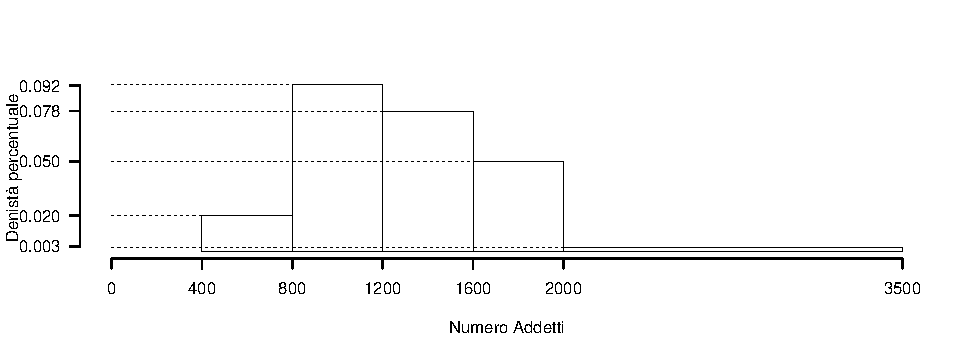
\includegraphics{Esami_passati_con_soluzioni_files/figure-latex/01-descr-23-1} \end{center}

\end{sol}

\subsection{Esercizio Dati non ordinati}\label{esercizio-dati-non-ordinati}

Con riferimento a molti processi industriali, si usa il
termine ``Work-In-Process'' (spesso abbreviato con WIP).
Negli impianti di produzione dei libri, il WIP rappresenta
il tempo necessario per piegare, riunire, cucire, e rilegare
i fogli che provengono da una pressa.
I dati che seguono sono relativi ai tempi di lavorazione
(tempo, in giorni, che intercorre tra quando i libri vengono
stampati e quando sono impacchettati nei cartoni) per due
campioni di 20 libri estratti da due impianti di produzione
(D. M. Levine \emph{et al}., 2000, \emph{Business Statistics:
A First Course}, 2.nd Edition, Prentice-Hall. Tr. it. (2002),
\emph{Statistica}, Apogeo, Milano, p.~126).

\begin{tabular}{lrrrrrrrrrr}
\toprule
Impianto 1 & 5.62 & 5.29 & 16.25 & 10.92 & 11.46 & 21.62 & 8.45 & 8.58 & 5.41 & 11.42\\
 & 11.62 & 7.29 & 7.50 & 7.96 & 4.42 & 10.50 & 7.58 & 9.29 & 7.54 & 8.92\\
Impianto 2 & 9.54 & 11.46 & 16.62 & 12.62 & 25.75 & 15.41 & 14.29 & 13.13 & 13.71 & 10.04\\
 & 5.75 & 12.46 & 9.17 & 13.21 & 6.00 & 2.33 & 14.25 & 5.37 & 6.25 & 9.71\\
\bottomrule
\end{tabular}

Determinare:

\begin{enumerate}
\def\labelenumi{\alph{enumi}.}
\tightlist
\item
  il campo di variazione,
\item
  la mediana,
\item
  la media sapendo che la somma è pari a 187.64 per l'impianto A e 227.07 per l'impianto B.
\end{enumerate}

\begin{sol}
Per rispondere alle tre domande conviene ordinare prima i dati, come
riportato nella tabella seguente.

\begin{tabular}{lrrrrrrrrrr}
\toprule
Impianto 1 & 4.42 & 5.29 & 5.41 & 5.62 & 7.29 & 7.50 & 7.54 & 7.58 & 7.96 & 8.45\\
 & 8.58 & 8.92 & 9.29 & 10.50 & 10.92 & 11.42 & 11.46 & 11.62 & 16.25 & 21.62\\
Impianto 2 & 2.33 & 5.37 & 5.75 & 6.00 & 6.25 & 9.17 & 9.54 & 9.71 & 10.04 & 11.46\\
 & 12.46 & 12.62 & 13.13 & 13.21 & 13.71 & 14.25 & 14.29 & 15.41 & 16.62 & 25.75\\
\bottomrule
\end{tabular}

Il campo di variazione è dato dalla differenza tra il massimo osservato
e il minimo.

\begin{eqnarray*}
\mbox{CdV}(A) &=& x_{A;\, (n)} - x_{A;\, (1)} = 21.62 - 4.42 = 17.2 \,. \\
\mbox{CdV}(B) &=& x_{B;\, (n)} - x_{B;\, (1)} = 25.75 - 2.33 = 23.42 \,.
\end{eqnarray*}

\begin{enumerate}
\def\labelenumi{\alph{enumi}.}
\item
  Il campo di variazione dell'impianto A è più piccolo di quello di B.
  Se le distribuzioni dei due insiemi di dati sono simili, allora ciò
  comporta un minore variabilità dei dati (o della prestazione)
  dell'impianto A.
\item
  La mediana per un numero di osservazioni pari è data da:
\end{enumerate}

\begin{eqnarray*}
x_{A;\, 0.5} &=& \frac{1} {2}\ \left( x_{A;\, (n/2)} + x_{A;\, (n/2)+1} \right)
              =  \frac{8.45 + 8.58} {2} = 8.515 \,. \\
x_{B;\, 0.5} &=& \frac{1} {2}\ \left( x_{B;\, (n/2)} + x_{B;\, (n/2)+1} \right)
              =  \frac{11.46 + 12.46} {2} = 11.96 \,.
\end{eqnarray*}

La mediana dell'impianto A è inferiore a quella dell'impianto B,
che comporta presumibilmente una diversa dislocazione (o non
sovrapponibilità) dei due istogrammi.

\begin{enumerate}
\def\labelenumi{\alph{enumi}.}
\setcounter{enumi}{2}
\tightlist
\item
  La media è data da:
\end{enumerate}

\begin{eqnarray*}
\bar{x}_{A} &=& \frac{187.64} {20} = 9.38 \,. \\
\bar{x}_{B} &=& \frac{227.07} {20} = 11.35 \,.
\end{eqnarray*}

Idem, come sopra: la media dell'impianto A è inferiore a quella
dell'impianto B, che comporta una diversa dislocazione (o non
sovrapponibilità) dei due istogrammi.
Tale esito mostra anche che l'impianto A è pi\textquotesingle u efficiente
dell'impianto B perché A produce in un tempo medio inferiore
a quello di B.

\end{sol}

\begin{enumerate}
\def\labelenumi{\alph{enumi}.}
\setcounter{enumi}{3}
\tightlist
\item
  \(\,\)il primo quartile,
\item
  \(\,\)il terzo quartile,
\item
  \(\,\)la differenza interquartile.
\end{enumerate}

\begin{sol}
Si ragiona sui dati ordinati sopra riportati.

\begin{enumerate}
\def\labelenumi{\alph{enumi}.}
\setcounter{enumi}{3}
\tightlist
\item
  Il primo quartile è dato dal valore della \(X\) relativa
  al soggetto nella posizione successiva a \(\lfloor n\, p \rfloor =
  \lfloor 20 \,\times\, 0.25 \rfloor = 5\), ossia \(x_{A;\, 0.25} =
  x_{A;\ (\lfloor n\, p \rfloor + 1)} = x_{A;\ (6)} = \textbf{7.50}\)
  e \(x_{B;\, 0.25} = x_{B;\ (\lfloor n\, p \rfloor + 1)} =
  x_{B;\ (6)} = \textbf{9.17}\).
  Si noti che il simbolo \(\lfloor \cdot \rfloor\) indica la parte
  intera dell'argomento.
  Tale regola è una approssimazione, adottata per semplificare
  il procedimento; tuttavia, in questo caso, si può ottenere un
  risultato pi\textquotesingle u preciso.
  Si tratta, infatti, di un numero divisibile per 4; pertanto, il
  primo quartile sarà dato dalla media dei valori corrispondenti
  ai soggetti 5.o e 6.o in graduatoria in modo da avere a sinistra
  esattamente 5 soggetti (il 25\%) e a destra 15 soggetti (il 75\%):
\end{enumerate}

\begin{eqnarray*}
x_{A;\, 0.25} &=& \frac{1} {2}\ \left( x_{A;\, (n/4)} + x_{A;\, (n/4)+1} \right)
               =  \frac{7.29 + 7.50} {2} = 7.395 \,. \\
x_{B;\, 0.25} &=& \frac{1} {2}\ \left( x_{B;\, (n/4)} + x_{B;\, (n/4)+1} \right)
               =  \frac{6.25 + 9.17} {2} = 7.71 \,.
\end{eqnarray*}

\begin{enumerate}
\def\labelenumi{\alph{enumi}.}
\setcounter{enumi}{4}
\tightlist
\item
  Il terzo quartile è dato dal valore della \(X\) relativa
  al soggetto nella posizione successiva a \(\lfloor n\, p \rfloor =
  \lfloor 20 \,\times\, 0.75 \rfloor = 15\), ossia \(x_{A;\, 0.75} =
  x_{A;\ (\lfloor n\, p \rfloor + 1)} = x_{A;\ (16)} = \textbf{11.42}\)
  e \(x_{B;\, 0.75} = x_{B;\ (\lfloor n\, p \rfloor + 1)} =
  x_{B;\ (16)} = \textbf{14.25}\).
  L'approssimazione è stata adottata, come già detto, per semplificare
  il procedimento, ma, in questo caso, si può ottenere un risultato pi\textquotesingle u
  preciso perché si tratta di un numero divisibile per 4; pertanto, il terzo
  quartile sarà dato dalla media dei valori corrispondenti ai soggetti 15.o
  e 16.o in graduatoria in modo da avere a sinistra esattamente 15 soggetti
  (il 75\%) e a destra 5 soggetti (il 15\%):
\end{enumerate}

\begin{eqnarray*}
x_{A;\, 0.75} &=& \frac{1} {2}\ \left( x_{A;\, (3n/4)} + x_{A;\, (3n/4)+1} \right)
               =  \frac{10.92 + 11.42} {2} = 11.17 \,. \\
x_{B;\, 0.75} &=& \frac{1} {2}\ \left( x_{B;\, (3n/4)} + x_{B;\, (3n/4)+1} \right)
               =  \frac{13.71 + 14.25} {2} = 13.98 \,.
\end{eqnarray*}

\begin{enumerate}
\def\labelenumi{\alph{enumi}.}
\setcounter{enumi}{5}
\tightlist
\item
  La differenza interquartile è data da:
\end{enumerate}

\begin{eqnarray*}
DI_{A} &=& x_{A;\, 0.75} - x_{A;\, 0.25} = 11.17 - 7.395 = 3.775 \,. \\
DI_{B} &=& x_{B;\, 0.75} - x_{B;\, 0.25} = 13.98 - 7.71  = 6.27 \,.
\end{eqnarray*}

\end{sol}

\begin{enumerate}
\def\labelenumi{\alph{enumi}.}
\setcounter{enumi}{6}
\tightlist
\item
  Calcolare la varianza, sapendo che
  \(\sum_{i=1}^{20} x_{A;\, i}^{2} = 2064.08\) e
  \(\sum_{i=1}^{20} x_{B;\, i}^{2} = 3077.31\).
\item
  Calcolare la deviazione standard.
\end{enumerate}

\begin{sol}

\begin{enumerate}
\def\labelenumi{\alph{enumi}.}
\setcounter{enumi}{6}
\tightlist
\item
  Per determinare la varianza, che è il quadrato della deviazione
  standard, si utilizza la formula che consente di ridurre gli errori
  di arrotondamento.
\end{enumerate}

\begin{eqnarray*}
\sigma_{A}^{2} &=& \frac{1} {n}\ \sum_{i=1}^{n} x_{i}^{2} - \bar{x}^{2}
                =  \frac{1} {20}\ 2064.08 - (9.38)^{2} = 15.18 \,. \\
\sigma_{B}^{2} &=& \frac{1} {n}\ \sum_{i=1}^{n} x_{i}^{2} - \bar{x}^{2}
                =  \frac{1} {20}\ 3077.31 - (11.35)^{2} = 24.96 \,.
\end{eqnarray*}

\begin{enumerate}
\def\labelenumi{\alph{enumi}.}
\setcounter{enumi}{7}
\tightlist
\item
  Per la deviazione standard si ha:
\end{enumerate}

\begin{eqnarray*}
\sigma_{A} &=& \sqrt{ \frac{1} {n}\ \sum_{i=1}^{n} x_{i}^{2} - \bar{x}^{2} }
            =  \sqrt{ \frac{1} {20}\ 2064.08 - (9.38)^{2} } = 3.90 \,. \\
\sigma_{B} &=& \sqrt{ \frac{1} {n}\ \sum_{i=1}^{n} x_{i}^{2} - \bar{x}^{2} }
            =  \sqrt{ \frac{1} {20}\ 3077.31 - (11.35)^{2} } = 5.00 \,.
\end{eqnarray*}

Idem, come sopra: la variabilità dei dati dell'impianto A è
inferiore a quella dell'impianto B, che comporta una maggiore
concentrazione dell'istogramma rafforzando le differenze (tra i
due impianti) già evidenziate.

\end{sol}

\begin{enumerate}
\def\labelenumi{\roman{enumi}.}
\tightlist
\item
  La distribuzione è asimmetrica?
  Se sì, di quale tipo di asimmetria si tratta?
\end{enumerate}

\begin{enumerate}
\def\labelenumi{\alph{enumi}.}
\setcounter{enumi}{9}
\tightlist
\item
  Dalle risposte date, emergono differenze tra i due impianti?
\end{enumerate}

\begin{sol}

\begin{enumerate}
\def\labelenumi{\roman{enumi}.}
\tightlist
\item
  La distribuzione dell'impianto A presenta una pronunciata
  asimmetria a destra (obliqua a destra o positiva), mentre quella
  dell'impianto B una minore asimmetria a sinistra (obliqua a sinistra
  o negativa).
  Per verificare numericamente questa affermazione si devono
  confrontare le media e la mediana:
\end{enumerate}

\begin{eqnarray*}
x_{A;\, 0.5} &=& 8.515\ <\ \bar{x}_{A}= 9.38 \quad\Rightarrow\quad
                 \mbox{obliqua (o asimmetrica) a destra} \\
x_{B;\, 0.5} &=& 11.96\ >\ \bar{x}_{B}= 11.35 \quad\Rightarrow\quad
                 \mbox{obliqua (o asimmetrica) a sinistra}\, .
\end{eqnarray*}

Si noti, tuttavia, che l'asimmetria a sinistra è poco evidente
perché lo scarto tra i due valori è solo di circa mezzo decimo
dell'unità, equivalente a circa il 5\% del valore della media.

\begin{enumerate}
\def\labelenumi{\alph{enumi}.}
\setcounter{enumi}{9}
\tightlist
\item
  Dalle risposte date si evincono alcune differenze:
\end{enumerate}

\begin{itemize}
\tightlist
\item
  la media dell'impianto A è inferiore di circa 2 punti;
\item
  la variabilità dell'impianto A è inferiore di quella di B;
\item
  l'asimmetria dell'impianto A è più pronunciata di quella di B.
\end{itemize}

Si può concludere che l'impianto A è più efficiente
dell'impianto B di circa due giorni e risulta anche più
``costante'' nella produzione perché il tempo di produzione
presenta una variabilità inferiore.

\end{sol}

\chapter{Esercizi di probabilità}\label{esercizi-di-probabilituxe0}

\section{Estrazioni con e senza reintroduzione}\label{estrazioni-con-e-senza-reintroduzione}

Un'urna contiene 3 bussolotti, due bianchi e uno nero.

1.a Si estrae \textbf{2 volte CON REINTRODUZONE} calcolare la probabilità che
la prima estrazione sia bianca e la seconda nera.

\begin{sol}
Indichiamo con

\begin{itemize}
\tightlist
\item
  \(E_1\) l'evento: esce bianco dall'estrazione 1
\item
  \(E_2\) l'evento: esce bianco dall'estrazione 2
\end{itemize}

l'evento \(E=\)\emph{``prima bianco e poi nero''} si scompone in

\[
E=E_1\cap\bar E_2
\]

ovvero \(E\) è vero se \(E_1\) è vero ed \(E_2\) è falso. Siccome le estrazioni sono
\textbf{con reintroduzione} allora le estrazioni sono indipendenti tra di loro e dunque

\begin{eqnarray*}
    P(E_1 \cap \bar E_2)
&=& P(E_1)P(\bar E_2)\\
&=& \frac{2}{3} \frac{1}{3}
 =  \frac{2}{9}
 =  0.22222.
\end{eqnarray*}

\end{sol}

1.b Si estrae \textbf{2 volte CON REINTRODUZONE} calcolare la probabilità di avere
una bianca e una nera, non importa l'ordine.

\begin{sol}
Indichiamo con

\begin{itemize}
\tightlist
\item
  \(E_1\) l'evento: esce bianco dall'estrazione 1
\item
  \(E_2\) l'evento: esce bianco dall'estrazione 2
\end{itemize}

l'evento \(F=\)\emph{``una bianca e una nera''} si scompone in

\[
F=(E_1\cap\bar E_2)\cup(\bar E_1\cap E_2)
\]

ovvero \(F\) è vero se \(E_1\) è vero ed \(E_2\) è falso OPPURE se \(E_1\) è falso ed \(E_2\) è vero.
Siccome le estrazioni sono \textbf{con reintroduzione} allora le estrazioni sono indipendenti
tra di loro e dunque

\begin{eqnarray*}
    P\big((E_1\cap\bar E_2)\cup(\bar E_1\cap E_2)\big)
&=& P(E_1)P(\bar E_2)+P(\bar E_1)P(E_2)\\
&=& \frac{2}{3} \frac{1}{3} + \frac{1}{3} \frac{2}{3} 
 =  \frac{4}{9}
 =  0.44444.
\end{eqnarray*}

\end{sol}

1.c Si estrae \textbf{2 volte SENZA REINTRODUZONE} calcolare la probabilità che
la prima estrazione sia bianca e la seconda nera.

\begin{sol}
Indichiamo con

\begin{itemize}
\tightlist
\item
  \(E_1\) l'evento: esce bianco dall'estrazione 1
\item
  \(E_2\) l'evento: esce bianco dall'estrazione 2
\end{itemize}

l'evento \(E=\)\emph{``prima bianco e poi nero''} si scompone in

\[
E=E_1\cap\bar E_2
\]

ovvero \(E\) è vero se \(E_1\) è vero ed \(E_2\) è falso. Siccome le estrazioni sono
\textbf{senza reintroduzione} allora le estrazioni \textbf{NON} sono indipendenti tra di loro e dunque

\begin{eqnarray*}
    P(E_1 \cap \bar E_2)
&=& P(E_1)P(\bar E_2|E_1)\\
&=& \frac{2}{3} \frac{1}{2}
 =  \frac{2}{6}
 =  0.33333.
\end{eqnarray*}

\end{sol}

1.d Si estrae \textbf{2 volte SENZA REINTRODUZONE} calcolare la probabilità di avere
una bianca e una nera, non importa l'ordine.

\begin{sol}
Indichiamo con

\begin{itemize}
\tightlist
\item
  \(E_1\) l'evento: esce bianco dall'estrazione 1
\item
  \(E_2\) l'evento: esce bianco dall'estrazione 2
\end{itemize}

l'evento \(F=\)\emph{``una bianca e una nera''} si scompone in

\[
F=(E_1\cap\bar E_2)\cup(\bar E_1\cap E_2)
\]

ovvero \(F\) è vero se \(E_1\) è vero ed \(E_2\) è falso OPPURE se \(E_1\) è falso ed \(E_2\) è vero.
Siccome le estrazioni sono \textbf{senza reintroduzione} allora le estrazioni \textbf{NON} sono indipendenti
tra di loro e dunque

\begin{eqnarray*}
    P\big((E_1\cap\bar E_2)\cup(\bar E_1\cap E_2)\big)
&=& P(E_1)P(\bar E_2|E_1)+P(\bar E_1)P(E_2|\bar E_1)\\
&=& \frac{2}{3} \frac{1}{2} + \frac{1}{3} \frac{2}{2} 
 =  \frac{2}{3}
 =  0.66667.
\end{eqnarray*}

\end{sol}

\section{Due urne}\label{due-urne}

Le scatole \(A\) e \(B\) contengono biglietti numerati.
La scatola \(A\) contiene un biglietto contrassegnato
con il numero 1 e tre biglietti con il numero 0.
La scatola \(B\) contiene tre biglietti contrassegnati
con il numero 1 e due con il numero 0.
Si effettua una estrazione da ognuna delle due scatole.

1.a Calcolare la probabilità di ottenere due biglietti
con il numero 1.

\begin{sol}
Indichiamo con

\begin{itemize}
\tightlist
\item
  \(A_0\) l'evento: esce 0 dall'urna \(A\)
\item
  \(A_1\) l'evento: esce 1 dall'urna \(A\)
\item
  \(B_0\) l'evento: esce 0 dall'urna \(B\)
\item
  \(B_1\) l'evento: esce 1 dall'urna \(B\)
\end{itemize}

Le due estrazioni danno origine a eventi tra loro
indipendenti e quindi

\begin{eqnarray*}
    P(A_1\cap B_1)
&=& P(A_1) P(B_1) \\
&=& \frac{1}{4} \times \frac{3}{5} = \frac{3}{20}.
\end{eqnarray*}

\end{sol}

1.b La probabilità che almeno uno dei biglietti sia
contrassegnato con il numero 1.

\begin{sol}
Si applica la regola dell'unione per eventi qualunque e si ha

\begin{eqnarray*}
    P(A_1 \cup B_1)
&=& P(A_1)+P(B_1)-P(A_1\cap B_1) \\
&=& \frac{1}{4}+ \frac{3}{5}-\frac{3}{20}
 =  \frac{14}{20}
 =  \frac{7}{10}  .
\end{eqnarray*}

Altro tipo di ragionamento o possibile soluzione: si applica la
regola del complementare all'evento C, \emph{almeno uno dei biglietti sia contrassegnato con il numero 1};
infatti, il complementare di
C è \emph{nessuno dei biglietti sia contrassegnato con il numero 1}.

\begin{eqnarray*}
    P(C)
&=& 1 - P(\overline{C}) \\
&=& 1 - \frac{3}{4}\ \frac{2}{5}
 =  \frac{14}{20}
 =  \frac{7}{10}  .
\end{eqnarray*}

Altro tipo di ragionamento (sconsigliato, in generale) è quello
di considerare tutti gli eventi possibili, l'evento \emph{almeno una estrazione con uno} è data da:

\begin{itemize}
\tightlist
\item
  \(C_{1}=A_1 \cap B_0\), unito a
\item
  \(C_{2}=A_0 \cap B_1\), unito a
\item
  \(C_{3}=A_1 \cap B_1\).
\end{itemize}

L'evento C, \emph{almeno uno dei biglietti sia contrassegnato con il numero 1} è dato dall'unione dei tre eventi, tra loro
\emph{incompatibili}

\begin{eqnarray*}
    P(C)
&=& P(C_{1} \cup C_{2} \cup C_{3}) \\
&=& P(C_{1}) + P(C_{2}) + P(C_{3}) \\
&=& \frac{1}{4}\ \frac{2}{5} + \frac{3}{4}\ \frac{3}{5} +
    \frac{1}{4}\ \frac{3}{5}
 =  \frac{14}{20}
 =  \frac{7}{10}  .
\end{eqnarray*}

\end{sol}

1.c La probabilità che la somma dei numeri riportati sui
biglietti estratti sia 1.

\begin{sol}
L'evento \lq\lq la somma dei due biglietti è 1'' può
essere scritta come

\begin{eqnarray*}
(A_1 \cup B_0) \cup (A_0 \cap B_1)
\end{eqnarray*}

e si ha

\begin{eqnarray*}
& & P[(A_1\cap B_0)\cup(A_0\cap B_1)] \\
&=& P(A_1\cap B_0) + P(A_0\cap B_1) \\
&=& P(A_1) P(B_0) + P(A_0) P(B_1) \\
&=& \frac{1}{4}\times \frac{2}{5} + \frac{3}{4}\times \frac{3}{5}
 =  \frac{11}{20}.
\end{eqnarray*}

\end{sol}

\section{Valigetta}\label{valigetta}

La serratura a combinazione di una valigia è composta da tre cifre.
Per aprire la valigia occorre scegliere un numero tra 1 e 9 per
ciascuna cifra.
Si ha a disposizione cinque soli tentativi, verificando l'apertura
a ogni combinazione.

1.a Qual è la probabilità di trovare la combinazione giusta
estraendo completamente a caso le tre cifre per un massimo di
cinque volte?

\begin{sol}
Il numero di combinazioni possibili è pari a \(9^{3}= 729\)
perché la stessa cifra si può ripetere nelle altre posizioni:
\emph{disposizioni con ripetizione}.

\begin{longtable}[]{@{}ll@{}}
\toprule\noalign{}
\(\#\) & tripletta \\
\midrule\noalign{}
\endhead
\bottomrule\noalign{}
\endlastfoot
1 & 1,1,1 \\
2 & 1,1,2 \\
\(\vdots\) & \(\vdots\) \\
9 & 1,1,9 \\
10 & 1,2,1 \\
\(\vdots\) & \(\vdots\) \\
81 & 1,9,9 \\
82 & 2,1,1 \\
\(\vdots\) & \(\vdots\) \\
729 & 9,9,9 \\
\end{longtable}

Per rispondere alla domanda si può costituire un'urna con
729 combinazioni e immaginare di estrarre da essa la
combinazione di ogni prova.

La stessa combinazione si può ripetere nella prova successiva
sicché l'esperimento è formato da estrazioni con reimmissione.
Sia \(C_{i}\) l'evento ``aprire'' nell'\(i\)-esimo tentativo.
Sarà \(\bar{C}_{i}\) l'evento complementare \emph{non aprire}
nell'\(i\)-esimo tentativo.

Sia \(B\) l'evento ``aprire in almeno cinque prove''.

\textbf{Soluzione diretta (lunga).}
L'evento \(B\)=``aprire in almeno cinque prove'' si può riscrivere come

\[
B=C_1\cup (\bar C_1\cap C_2)\cup (\bar C_1\cap \bar C_2\cap C_3) \cup (\bar C_1\cap \bar C_2\cap \bar C_3\cap C_4)\cup (\bar C_1\cap \bar C_2\cap \bar C_3\cap\bar C_4\cap C_5)
\]

che si legge: per aprire in almeno cinque tentativi:

\begin{itemize}
\tightlist
\item
  apro al primo \(C_1\), oppure \(\cup\)
\item
  non apro al primo e apro al secondo \((\bar C_1\cap C_2)\)
\item
  \ldots{}
\item
  non apro al primo, non apro al secondo, \ldots, apro al quinto \((\bar C_1\cap \bar C_2\cap \bar C_3\cap\bar C_4\cap C_5)\)
\end{itemize}

e quindi

\[\begin{array}{lll}
P(B)   &=&  P\Big(C_1\cup (\bar C_1\cap C_2) \cup (\bar C_1\cap \bar C_2\cap C_3)\cup \\
&& \qquad\cup(\bar C_1\cap \bar C_2\cap \bar C_3\cap C_4)\cup (\bar C_1\cap \bar C_2\cap \bar C_3\cap\bar C_4\cap C_5)\Big)\\
&=& P(C_1)+P(\bar C_1\cap C_2)+P(\bar C_1\cap \bar C_2\cap C_3)+\\
&&\qquad + P(\bar C_1\cap \bar C_2\cap \bar C_3\cap C_4)+P(\bar C_1\cap \bar C_2\cap \bar C_3\cap\bar C_4\cap C_5)\\
&=& P(C_1)+P(\bar C_1) P( C_2)+P(\bar C_1) P( \bar C_2) P( C_3)+ \\
&&\qquad+P(\bar C_1) P( \bar C_2) P( \bar C_3) P( C_4)+P(\bar C_1) P( \bar C_2) P( \bar C_3) P(\bar C_4) P( C_5)\\
&=& \frac 1{729} + \frac {728}{729}\frac {1}{729} + \left(\frac {728}{729}\right)^2\frac {1}{729}
+ \left(\frac {728}{729}\right)^3\frac {1}{729}+ \left(\frac {728}{729}\right)^4\frac {1}{729}\\
&=& 0.00684
\end{array}\]

\textbf{Soluzione indiretta (corta).}
Il calcolo diventa facile se si applica la regola del complementare:
si calcola la probabilità dell'evento \(\bar{B}\), ``non aprire nei
cinque tentativi''.

\begin{eqnarray*}
P(B)&=& 1 - P(\bar{B}) \\
    &=& 1 - P(\bar{C}_{1} \cap \bar{C}_{2} \cap \bar{C}_{3} \cap
              \bar{C}_{4} \cap \bar{C}_{5}) \\
    &=& 1 - P(\bar{C}_{1}) P(\bar{C}_{2}) P(\bar{C}_{3}) 
            P(\bar{C}_{4}) P(\bar{C}_{5}) \\
    &=& 1 - \left( \frac{728} {729} \right)^{5}
     =  1 - 0.99316 = 0.00684  .
\end{eqnarray*}

\end{sol}

1.b Qual è la probabilità di trovare la combinazione giusta
estraendo completamente a caso le tre cifre per un massimo di
cinque volte tenendo conto delle combinazioni già provate?

\begin{sol}
Il numero di combinazioni possibili è pari a \(9^{3}= 729\) (v. sopra).
Per rispondere alla domanda si costituisce sempre un'urna con 729
combinazioni e si estrae da essa la combinazione di ogni prova,
ma le combinazioni provate non vengono reimmesse nell'urna per
non ripescarle nei tentativi successivi.

Sia \(C_{i}\) l'evento ``aprire'' nell'\(i\)-esimo tentativo.
Sia \(\bar{C}_{i}\) l'evento complementare ``non aprire''
nell'\(i\)-esimo tentativo.

\textbf{Soluzione diretta (lunga).}
L'evento \(B\)=``aprire in almeno cinque prove'' si può riscrivere come

\[
B=C_1\cup (\bar C_1\cap C_2)\cup (\bar C_1\cap \bar C_2\cap C_3)\cup (\bar C_1\cap \bar C_2\cap \bar C_3\cap C_4)\cup (\bar C_1\cap \bar C_2\cap \bar C_3\cap\bar C_4\cap C_5)
\]

che si legge: per aprire in almeno cinque tentativi:

\begin{itemize}
\tightlist
\item
  apro al primo \(C_1\), oppure \(\cup\)
\item
  non apro al primo e apro al secondo \((\bar C_1\cap C_2)\)
\item
  \ldots{}
\item
  non apro al primo, non apro al secondo, \ldots, apro al quinto \((\bar C_1\cap \bar C_2\cap \bar C_3\cap\bar C_4\cap C_5)\)
\end{itemize}

e quindi

\[\begin{array}{lll}
P(B)   &=&  P\Big(C_1\cup (\bar C_1\cap C_2) \cup (\bar C_1\cap \bar C_2\cap C_3)\cup \\
&& \qquad\cup(\bar C_1\cap \bar C_2\cap \bar C_3\cap C_4)\cup (\bar C_1\cap \bar C_2\cap \bar C_3\cap\bar C_4\cap C_5)\Big)\\
&=& P(C_1)+P(\bar C_1\cap C_2)+P(\bar C_1\cap \bar C_2\cap C_3)+\\
&&\qquad + P(\bar C_1\cap \bar C_2\cap \bar C_3\cap C_4)+P(\bar C_1\cap \bar C_2\cap \bar C_3\cap\bar C_4\cap C_5)\\
&=& P(C_1)+P(\bar C_1) P( C_2|\bar C_1)+P(\bar C_1) P( \bar C_2|\bar C_1) P( C_3|\bar C_1\cap \bar C_2)+ \\
&&\qquad+P(\bar C_1) P( \bar C_2|\bar C_1) P( C_3|\bar C_1\cap \bar C_2)P( C_4|\bar C_1\cap \bar C_2\cap\bar C_3)+\\
&&\qquad+P(\bar C_1) P( \bar C_2|\bar C_1) P( C_3|\bar C_1\cap \bar C_2)P( C_4|\bar C_1\cap \bar C_2\cap\bar C_3)\cdot\\
&&\qquad\quad\cdot P( C_5|\bar C_1\cap \bar C_2\cap\bar C_3\cap C_4)\\
&=& \frac 1{729} + \frac {728}{729}\frac {1}{728} + \frac {728}{729}\frac {727}{728}\frac {1}{727}+\frac {728}{729}\frac {727}{728}\frac {726}{727}\frac {1}{726}+\\
&&\qquad +\frac {728}{729}\frac {727}{728}\frac {726}{727}\frac {725}{726}\frac{1}{725}\\
&=&\frac 5{729}\\
&=& 0.00686
\end{array}\]

\textbf{Soluzione indiretta (corta).}
Sia B l'evento ``aprire in almeno cinque prove''.
Il calcolo diventa facile se si applica la regola del complementare:
si calcola la probabilità dell'evento \(\bar{B}\), ``non aprire nei
cinque tentativi''.

\begin{eqnarray*}
 P(B) &=& \\
&=& 1 - P(\bar{B})
 =  1 - P(\bar{C}_{1} \cap \bar{C}_{2} \cap \bar{C}_{3} \cap
          \bar{C}_{4} \cap \bar{C}_{5}) \\
&=& 1 - P(\bar{C}_{1}) P(\bar{C}_{2}  |  \bar{C}_{1})  
        P(\bar{C}_{3}  |  \bar{C}_{1}, \bar{C}_{2})  
        P(\bar{C}_{4}  |  \bar{C}_{1}, \bar{C}_{2}, \bar{C}_{3})  
        P(\bar{C}_{5}  |  \bar{C}_{1}, \bar{C}_{2}, \bar{C}_{3}, \bar{C}_{4}) \\
&=& 1 - \frac{728} {729}\ \frac{727} {728}\ \frac{726} {727}\ \frac{725} {726}\ \frac{724} {725}
 =  1 - 0.99314 = 0.00686  .
\end{eqnarray*}

\end{sol}

\section{Urna}\label{urna}

Si supponga di estrarre a caso e SENZA reimmissione (ESR) 2 palline
da un'urna contenente 5 palline rosse e 10 palline gialle.
Si considerino gli eventi seguenti:

\begin{itemize}
\tightlist
\item
  A=\{pallina rossa alla prima estrazione (colore qualsiasi alla seconda)\},
\item
  B=\{pallina rossa alla seconda estrazione (colore qualsiasi alla prima)\},
\item
  C=\{pallina gialla alla seconda estrazione (colore qualsiasi alla prima)\}.
\end{itemize}

1.a Quali sono le coppie di palline che formano l'unione
degli eventi A e B, ovvero \((A \cup B)\)?

\begin{itemize}
\tightlist
\item
  \(\Box\) Coppie contenenti due palline gialle.
\item
  \(\Box\) Coppie contenenti esattamente una pallina rossa.
\item
  \(\Box\) Coppie contenenti almeno una pallina rossa.
\item
  \(\Box\) Coppie contenenti due palline rosse.
\end{itemize}

\begin{sol}
Coppie contenenti almeno una pallina rossa

\end{sol}

1.b Quali sono le coppie di palline che formano l'intersezione
degli eventi A e B, ovvero (A \(\cap\) B)?

\begin{itemize}
\tightlist
\item
  \(\Box\) Coppie contenenti due palline gialle.
\item
  \(\Box\) Coppie contenenti al più una pallina rossa.
\item
  \(\Box\) Coppie contenenti almeno una pallina rossa.
\item
  \(\Box\) Coppie contenenti due palline rosse.
\end{itemize}

\begin{sol}
Coppie contenenti due palline rosse

\end{sol}

1.c Qual è il complementare di C?

\begin{sol}
\(\overline{C}=B\)

\end{sol}

1.d Calcolare la probabilità di C condizionata all'evento A, \(P(C|A).\)

\begin{sol}
Noto che A si è verificato, nell'urna rimangono 14 palline di cui 4 sono rosse
e 10 sono gialle: \(P(C|A)= 10/14 = 0.714.\)

\end{sol}

\section{Applicazione regole}\label{applicazione-regole}

La probabilità dell'evento A è 1/3.
La probabilità dell'evento B è 1/2.
I due eventi sono indipendenti.

1.a Calcolare P(\(\overline{B}\)).

\begin{sol}
P(\(\overline{B}\))= 1 - P(B)=1/2

\end{sol}

1.b Calcolare la probabilità che si verifichi B,
dato che A si è verificato.

\begin{sol}
Dal momento che i due eventi sono indipendenti, la probabilità
condizionata coincide con la probabilità semplice.
In alternativa si può procedere al calcolo nel modo seguente:

\[P({B}|A)= \frac{P(B \cap A)}{P(A)} = \frac{P(B) \times P(A)}{P(A)} = P({B}) =1/2\]

\end{sol}

1.c I due eventi sono incompatibili?

\begin{sol}
No, perché \({P(A \cap B)}\) = \({P(A) \times P(B)}\) =1/3 \(\times\) 1/2 = 1/6 \(\neq\) 0.

\end{sol}

\section{Studente}\label{studente}

Uno studente arriva a un esame avendo studiato 20 dei 25
argomenti del corso.
L'insegnante gli pone 3 domande su argomenti diversi e
l'esame è superato solo se tutte le risposte sono giuste.

1.a Qual è la probabilità che lo studente
superi l'esame al primo appello?

\begin{sol}
Per superare l'esame lo studente deve conoscere tutte e
tre gli argomenti richiesti.
Tale problema equivale a estrarre tre palline da un'urna
che ne contiene 25 (di cui 20 di colore verde -- argomenti noti --
e 5 di colore rosso -- argomenti non studiati).
Dal momento che si specifica che le tre domande sono relative a
argomenti diversi, le estrazioni delle tre palline devono essere
effettuate SENZA reimmissione.
In questo caso lo studente deve estrarre
tre palline verdi in tre estrazioni.
La probabilità cercata è data da

\[
P(\mbox{conoscere tutte e tre le risposte})=
\frac{20}{25} \times \frac{19}{24} \times \frac{18}{23} = 0.49565  .
\]

\end{sol}

1.b Qual è la probabilità che lo studente superi
l'esame nella prima sessione (in cui ci sono tre appelli)?
Si assuma che gli eventi ``superamento dell'esame'' siano
indipendenti, anche se l'assunto non è realistico.

\begin{sol}
\textbf{Soluzione diretta (lunga).}
Sia \(A_{i}\) la probabilità di superare l'esame nell'\(i\)-esimo
appello e \(\bar{A}_{i}\) è la probabilità di non superarlo.
L'evento \(B\), superare entro il terzo appello, si può scomporre come

\[B=A_1\cup(\bar A_1\cap A_2)\cup(\bar A_1\cap\bar A_2\cap A_3)\]

e quindi

\begin{eqnarray*}
  P(B) &=& P(A_1\cup(\bar A_1\cap A_2)\cup(\bar A_1\cap\bar A_2\cap A_3))\\
       &=& P(A_1)+P(\bar A_1\cap A_2)+P(\bar A_1\cap\bar A_2\cap A_3)\\
       &=& P(A_1)+P(\bar A_1)P( A_2)+P(\bar A_1)P(\bar A_2)P( A_3)\\ 
       &=& 0.49565+(1-0.49565)\times 0.49565 + (1-0.49565)^2\times 0.49565\\
       &=& 0.87171
\end{eqnarray*}

\textbf{Soluzione indiretta (corta).}
La probabilità di superare l'esame entro la sessione, evento \(B\)
si calcola facilmente applicando la regola del complementare nel
quale \(\bar{B}\) è la probabilità di non superare l'esame nella
sessione:

\begin{eqnarray*}
P(B) &=& 1- P(\bar{B})
      =  1- P(\bar{A}_{1} \cap \bar{A}_{2} \cap \bar{A}_{3}) \\
     &=& 1- P(\bar{A}_{1}) P(\bar{A}_{2}  |  \bar{A}_{1}) 
            P(\bar{A}_{3}  |  \bar{A}_{1}, \bar{A}_{2}) \\
     &=& 1- \left( 1-0.49565 \right)^{3} = 1 - 0.12829= 0.87171  .
\end{eqnarray*}

\end{sol}

\section{Giulio e il treno}\label{giulio-e-il-treno}

Giulio deve prendere il treno, ma non ha molto tempo: per
raggiungere la stazione decide di aspettare l'autobus che
arriverà puntualmente (evento \(A\)) con probabilità pari a 0.7.
Arrivato in stazione puntualmente, riuscirà a salire sul
treno evitando la multa del controllore se non troverà
coda alla biglietteria (evento \(B\)).
Questo accade con probabilità pari a 0.5.

1.a Calcolare la probabilità che Giulio non debba pagare
la multa (evento \(C\)).

\begin{sol}
Giulio sale sul treno senza prendere la multa solo se simultaneamente
si verificano due eventi (indipendenti): l'autobus è puntuale
(evento \(A\)) e non c'è coda in biglietteria (evento \(B\)).
La probabilità cercata si ottiene allora applicando la regola del
prodotto (per eventi indipendenti):

\begin{eqnarray*}
P(C) &=& P(A \cap B) = P(A) P(B) = 0.7 \times 0.5 = 0.35  .
\end{eqnarray*}

\end{sol}

1.b Calcolare la probabilità che Giulio in tre giorni
diversi riesca a evitare almeno una multa (evento \(D\)).

\begin{sol}
La probabilità di evitare almeno una multa in tre giorni si
può calcolare ricorrendo alla regola del complementare.
L'evento \(D\) si ottiene dalle diverse combinazioni dell'evento
\(C_{i}\) e \(\bar{C}_{i}\) giornalieri.

La probabilità di \(C_{i}\) è stata calcolata in precedenza.
Il complementare di \(D\), è \(\bar{D}\) che indica l'evento
``paga sempre la multa'', allora si ha

\begin{eqnarray*}
P(D) &=& 1 - P(\bar{D})
      =  1 - P(\bar{C}_{1} \cap \bar{C}_{2} \cap \bar{C}_{3}) \\
     &=& 1 - P(\bar{C}_{1}) P(\bar{C}_{2}) P(\bar{C}_{3})
      =  1 - (1- 0.35) (1- 0.35) (1- 0.35) \\
     &=& 1-0.274625 = 0.725375  .
\end{eqnarray*}

\end{sol}

\section{Somma di due dadi}\label{somma-di-due-dadi}

Si lancia una coppia di dadi.

1.a Costruire il supporto.

\begin{sol}
Il supporto della coppia di VC, si ottiene con una tabella a
doppia entrata, nella quale sulle righe si mettono i risultati
del primo dado (\(D1\)) e sulle colonne si mettono i risultati
del secondo dado (\(D2\)).

Lo spazio \(\Omega\) consiste di 36 \emph{combinazioni equiprobabili}.

\end{sol}

1.b Determinare la probabilità di un
punto del supporto.

\begin{sol}
Presa una qualunque coppia (\(\fbox{4}\), \(\fbox{2}\)),
i due eventi sono ``fisicamente'' \emph{indipendenti} sicché

\[
    P(\fbox{4}  ,\ \fbox{2})
= P(\fbox{4}) P(\fbox{2}) = \frac{1} {6}  \times  \frac{1} {6}
= \frac{1} {36}
\]

La risposta era anche intuitiva perché gli eventi di \(\Omega\)
sono equiprobabili: 1/36.

\end{sol}

1.c Qual è la probabilità che la somma dei punteggi sia 9?

\begin{sol}
Si può procedere al conteggio degli eventi che danno somma, \(S\), pari a 9:

\[
P(S=9) = 4  \times  \frac{1} {36} = \frac{1} {9}
\]

Si noti che la probabilità di avere 3 è

\begin{eqnarray*}
    P(\text{un dado $\fbox{2}$ e un dado $\fbox{1}$})
&=& P\left( (\lbrace \fbox{2}\rbrace \cap \lbrace \fbox{1}\rbrace) \cup
            (\lbrace \fbox{1}\rbrace \cap \lbrace \fbox{2}\rbrace)
    \right) \\
&=& P(\fbox{2}\ \fbox{1}) + P(\fbox{1}\ \fbox{2}) = \frac{2} {36}   .
\end{eqnarray*}

Nell'evento non si è specificato l'ordine con cui devono uscire
i due dadi \(\Rightarrow\) bisogna considerare le diverse possibilità.
Si noti, poi, che gli eventi \(\{\fbox{2}\ \fbox{1}\}\) e
\(\{\fbox{1}\ \fbox{2}\}\) sono tra loro \emph{incompatibili}:
si verifica l'uno \emph{o} (esclusivo -- XOR) si verifica l'altro.

\end{sol}

1.d Qual è la probabilità che la somma (\(S\))
dei punteggi di due dadi sia minore di quattro?

\begin{sol}
Si tratta della somma di eventi incompatibili: \(\{S=2\}\) \emph{e} \(\{ S=3 \})\):

\begin{eqnarray*}
P(S<4) &=& P(\{S=2\} \cup \{ S=3 \})
        =  P(\{S=2\}) + P(\{ S=3 \}) \\
       &=& \frac{1} {36} + \frac{2} {36} = \frac{1} {12}   .
\end{eqnarray*}

\end{sol}

1.e Calcolare la probabilità che la SOMMA (\(S\))
dei punteggi di due dadi sia pari a sette oppure
uno dei dadi sia pari a sei (\(U6\)).

\begin{sol}
\begin{eqnarray*}
P(S=7) &=& P(\{\fbox{1}\ \fbox{6}\} \cup  \cdots \cup \{\fbox{6}\ \fbox{1}\})
        =  \frac{6} {36} \\
P(U=6) &=& P(\{\fbox{1}\ \fbox{6}\} \cup  \cdots \cup \{\fbox{6}\ \fbox{1}\})
        = \frac{11} {36} \\
       &:& \{ S=7 \}\quad e \quad \{ U=6 \}\quad \mbox{non sono incompatibili}
           \quad\rightarrow \\[0.2cm]
           P(\{ S=7 \} \cup \{ U=6 \})
       &=& P(\{ S=7 \}) +  P(\{ U=6 \}) - P(\{ S=7 \} \cap \{ U=6 \}) \\
       &=& \frac{6} {36} + \frac{11} {36} - \frac{2} {36}
        =  \frac{15} {36} \qquad \mbox{infatti} \quad\rightarrow    \\
           P(\{ S=7 \} \cap \{ U=6 \})
       &=& \{ \fbox{1}\ \fbox{6} \} \cup \{ \fbox{6}\ \fbox{1} \}
           \qquad \mbox{tra loro incompatibili}   .
\end{eqnarray*}

Dati DUE eventi \(A\) e \(B\), la probabilità dell'UNIONE (\(A\cup B\))
è uguale alla somma delle probabilità dei singoli eventi, MENO
la probabilità della loro intersezione

\[
P(A \cup B) = P(A) + P(B) - P(A \cap B)  .
\]

Se \(A\) e \(B\) sono incompatibili, allora
\(A \cap B = \emptyset \Rightarrow P(A \cap B)=P(\emptyset)=0\). \textbackslash{}

\end{sol}

\section{Scatola e biglietti}\label{scatola-e-biglietti}

La scatola \(A\) contiene 4 biglietti numerati da 1 a 4.
La scatola \(B\) contiene 3 biglietti numerati da 2 a 4.
Si estrae un biglietto da ognuna delle scatole e si indica
con \(A_{1}\) il valore del biglietto estratto dalla scatola \(A\) e
con \(B_{1}\) quello della scatola \(B\).

1.a Ricavare la distribuzione di probabilità di \(X=A_{1}+B_{1}\).

\begin{sol}

Lo spazio campionario dell'esperimento considerato è costituito
da \(4\times 3=12\) coppie equiprobabili di biglietti:

\begin{eqnarray*}
\{(1,2); (1,3); (1,4); (2,2); (2,3); (2,4); (3,2); (3,3); (3,4); (4,2); (4,3); (4,4)\}.
\end{eqnarray*}

Sommando i due termini di ogni coppia si ricava facilmente
che la distribuzione di probabilità di \(X\) è

\begin{tabular}{llll}
\toprule
  & $B_2=2$ & $B_2=3$ & $B_2=4$\\
\midrule
$A_1=1$ & $3;\frac 1{12}$ & $4;\frac 1{12}$ & $5;\frac 1{12}$\\
$A_1=2$ & $4;\frac 1{12}$ & $5;\frac 1{12}$ & $6;\frac 1{12}$\\
$A_1=3$ & $5;\frac 1{12}$ & $6;\frac 1{12}$ & $7;\frac 1{12}$\\
$A_1=4$ & $6;\frac 1{12}$ & $7;\frac 1{12}$ & $8;\frac 1{12}$\\
\bottomrule
\end{tabular}

da cui la probabilità di \(X\)

\begin{tabular}{lr}
\toprule
X & Freq\\
\midrule
3 & 0.08333\\
4 & 0.16667\\
5 & 0.25000\\
6 & 0.25000\\
7 & 0.16667\\
8 & 0.08333\\
\bottomrule
\end{tabular}

\end{sol}

1.b Calcolare la probabilità dell'evento \(\{A_{1}>B_{1}\}\).

\begin{sol}

Dallo spazio campionario presentato nel punto (a)
si vede che il valore del primo biglietto è superiore
a quello del secondo solo in \(3\) delle \(12\) coppie
e quindi \(P(A_{1}>B_{1})=1/4\).

\begin{tabular}{llll}
\toprule
  & $B_2=2$ & $B_2=3$ & $B_2=4$\\
\midrule
$A_1=1$ & $0;\frac 1{12}$ & $0;\frac 1{12}$ & $0;\frac 1{12}$\\
$A_1=2$ & $0;\frac 1{12}$ & $0;\frac 1{12}$ & $0;\frac 1{12}$\\
$A_1=3$ & $1;\frac 1{12}$ & $0;\frac 1{12}$ & $0;\frac 1{12}$\\
$A_1=4$ & $1;\frac 1{12}$ & $1;\frac 1{12}$ & $0;\frac 1{12}$\\
\bottomrule
\end{tabular}

\end{sol}

1.c Si ripete l'esperimento 10 volte reinserendo i biglietti
estratti nelle rispettive scatole dopo ogni estrazione.
Calcolare la probabilità che il valore del biglietto della
scatola \(A\) sia superiore a quello della scatola \(B\) in meno
di 4 delle 10 estrazioni.

\begin{sol}
Ad ogni ripetizione dell'esperimento la probabilità che
il biglietto estratto da \(A\) riporti un valore superiore
a quello del biglietto estratto da \(B\) è 1/4.
Il numero di volte che questo evento si verifica in 10
replicazioni indipendenti dell'esperimento è un numero
aleatorio \(S\), distribuito secondo una binomiale,
\(S\sim \mbox{Bin}(10;  1/4)\); quindi, la probabilità
cercata è

\[
P(S<4)
= \sum_{i=0}^{3} \binom{10}{i} (0.25)^{i} (1-0.25)^{10-i}
= 0.776  .
\]

\end{sol}

\section{Urna con colori e lettere diverse}\label{urna-con-colori-e-lettere-diverse}

Un'urna contiene 3 palline rosse timbrate con \(\color{red}{\mbox{A}}\), 2 palline rosse timbrate con \(\color{red}{\mbox{B}}\), 1 palline rossa timbrate con \(\color{red}{\mbox{C}}\), 2 palline verdi timbrate con \(\color{green}{\mbox{A}}\), una verde con \(\color{green}{\mbox{B}}\), una verde con \(\color{green}{\mbox{C}}\), una nera con \(\color{black}{\mbox{A}}\) e una nera con \(\mbox{C}\).
In tabella

\begin{tabular}{>{}l|rrr|>{}r}
\toprule
 & A & B & C & Tot\\
\midrule
\textbf{Rosso} & 3 & 2 & 1 & \textbf{6}\\
\textbf{Verde} & 2 & 1 & 1 & \textbf{4}\\
\textbf{Nero} & 1 & 0 & 1 & \textbf{2}\\
\midrule
\textbf{\textbf{Tot}} & \textbf{6} & \textbf{3} & \textbf{3} & \textbf{\textbf{12}}\\
\bottomrule
\end{tabular}

1.a Calcolare la probabilità di estrarre una pallina Rossa

\begin{sol}
Sia
\[
R = \text{estraggo Rosso}
\]
\[
P(R)=\frac6{12}=0.5
\]

\end{sol}

1.b Calcolare la probabilità di estrarre una pallina timbrata con \(\mbox{A}\)

\begin{sol}
Sia
\[
A = \text{estraggo una pallina timbrata con $\mbox{A}$}
\]
\[
P(A)=\frac6{12}=0.5
\]

\end{sol}

1.c Gli eventi \(A\) ed \(R\) sono indipendenti?

\begin{sol}
Sì, in quanto
\[
P(A\cap R)=\frac1{4}=\frac12\cdot\frac12=P(A)P(R)
\]
e quindi
\[
P(A|R)=\frac{P(A\cap R)}{P(R)}=\frac{\frac{1}{4}}{\frac12}=\frac 12= P(A)
\]
e viceversa
\[P(R|A)=\frac{P(A\cap R)}{P(A)}=\frac{\frac{1}{4}}{\frac12}=\frac 12= P(R)\]

\end{sol}

1.d Calcolare la probabilità di estrarre una pallina verde

\begin{sol}
Sia
\[
V = \text{estraggo una pallina verde}
\]
\[
P(V)=\frac4{12}=\frac13
\]

\end{sol}

1.e Gli eventi \(V\) ed \(R\) sono indipendenti?

\begin{sol}
\textbf{NO} \(V\) e \(R\) sono \textbf{incompatibili}, se la pallina è uscita verde \textbf{non} può essere rossa

\[
P(V\cap R)=P(\emptyset)=0
\]

\end{sol}

1.f Gli eventi \(V\) ed \(A\) sono indipendenti?

\begin{sol}
Sì, in quanto
\[
P(V\cap A)=\frac2{12}=\frac13\cdot\frac12=P(V)P(A)
\]
e quindi
\[
P(V|A)=\frac{P(V\cap A)}{P(A)}=\frac{\frac{1}{3}}{\frac12}=\frac 12= P(V)
\]

\emph{Interpretazione} Sapere se la pallina estratta è targata con A non cambia il nostro stato informativo
sul colore, viceversa, sapere il colore non cambia il nostro stato informativo sul fatto che sia timbrata A.

\end{sol}

1.g Calcolare \(P(N)\) (probabilità di estrarre nera) e \(P(B)\) (probabilità di estrarre una pallina timbrata con B)

\begin{sol}
\begin{eqnarray*}
P(N)   &=&  \frac2{12}=\frac16\\
P(B)   &=& \frac3{12}
\end{eqnarray*}

\end{sol}

1.h Gli eventi \(B\) ed \(N\) sono indipendenti?

\begin{sol}
\textbf{NO} \(B\) e \(N\) sono \textbf{incompatibili}, se la pallina è uscita nera \textbf{non} può essere timbrata con B

\[P(B\cap N)=\frac0{12}=0\]

\end{sol}

1.i Gli eventi \(C\) (estrarre una pallina con C) ed \(N\) sono indipendenti?

\begin{sol}
\textbf{No}, in quanto
\[
P(C)=\frac3{12}=\frac14
\]
mentre
\[
P(C\cap N)=\frac1{12}\neq \frac{3}{12}\cdot\frac2{12}=P(C)P(N)
\]
e quindi
\[
P(C|N)=\frac12\neq\frac14=P(C)
\]

\end{sol}

1.j Gli eventi \(B\) ed \(N\) sono incompatibili?

\begin{sol}
\textbf{No}, in quanto
\[
P(C\cap N)=\frac1{12}\neq 0
\]

\end{sol}

\section{Urne che portano ad altre urne}\label{urne-che-portano-ad-altre-urne}

Si consideri il seguente gioco: si estrae una dall'urna \(U\) che contiene 2 palline Rosse e una pallina Bianca:
\small

\begin{itemize}
\tightlist
\item
  \textbf{se} esce Rossa si estrae da un'urna che ha 3 palline marcate con A e 1 pallina marcata con B
\item
  \textbf{se} esce Bianca si estrae da un'urna che ha 1 pallina marcata con A e 1 pallina marcata con B
\end{itemize}

\rm

1.a Qual è la probabilità di osservare una pallina marcata con A?

\begin{sol}
Anzitutto osserviamo che
\begin{eqnarray*}
  P(R) &=&  \frac23\\
  P(B) &=& \frac13
\end{eqnarray*}

e che

\begin{eqnarray*}
  P(A|R) &=&  \frac34\\
  P(A|B) &=& \frac12
\end{eqnarray*}

e quindi

\begin{eqnarray*}
  P(A) &=&  P(R)P(A|R)+P(B)P(A|B)\\
   &=& \frac23\frac34+\frac13\frac12\\
   &=& \frac23\\
   &=& 0.66667
\end{eqnarray*}

\end{sol}

1.b Sapendo che è uscita una pallina marcata con A, qual è la probabilità che all'inizio del gioco sia stata estratta la pallina Rossa?

\begin{sol}
\begin{eqnarray*}
  P(R|A)  &=&  \frac{P(A\cap R)}{P(A)}\\
          &=&  \frac{P(R)P(A|R)}{P(A)}\\
          &=&  \frac{\frac23\frac34}{\frac23}\\
          &=&  \frac34\\
          &=& 0.75
\end{eqnarray*}

\end{sol}

\section{Estrazioni con e senza reintroduzione (continua)}\label{estrazioni-con-e-senza-reintroduzione-continua}

Un'urna contiene 3 palline Rosse, 2 Bianche e 5 Verdi,

1.a si estrae 3 volte \textbf{con} reintroduzione.
Calcolare la probabilità di aver 3 colori diversi

\begin{sol}

Anzitutto notiamo che l'evento
\[
E=\text{“tre colori diversi”}
\]
si scompone come
\begin{eqnarray*}
  E     &=&  (R\cap B\cap V)\cup(R\cap V\cap B)\cup\\
        &=&  (B\cap E\cap V)\cup(B\cap V\cap R)\cup\\
        &=&  (V\cap R\cap B)\cup(V\cap B\cap R)
\end{eqnarray*}
e quindi
\begin{eqnarray*}
  P(E)  &=& P(R\cap B\cap V)+P(R\cap V\cap B)+\\
        &=& P(B\cap E\cap V)+P(B\cap V\cap R)+\\
        &=& P(V\cap R\cap B)+P(V\cap B\cap R)
\end{eqnarray*}

notiamo che le estrazioni sono tra di loro \textbf{indipendenti} e quindi

\begin{eqnarray*}
  P(E)  &=& P(R)P(B)P(V)+P(R)P(V)P(B)+\\
        &=& P(B)P(R)P(V)+P(B)P(V)P(R)+\\
        &=& P(V)P(R)P(B)+P(V)P(B)P(R)\\
        &=& \frac2{10}\frac5{10}\frac3{10}+\frac2{10}\frac3{10}\frac5{10}+...\\
        &=& 6 \cdot \frac2{10}\frac5{10}\frac3{10}\\
        &=& 0.18
\end{eqnarray*}

\begin{nota}
\(6=3!\) è il numero di modi in cui posso mescolare i tre colori

\end{nota}

\end{sol}

1.b si estrae 3 volte \textbf{senza} reintroduzione.
Calcolare la probabilità di aver 3 colori diversi.

\begin{sol}
in questo caso le estrazioni \textbf{non} sono tra di loro \textbf{indipendenti} e quindi

\begin{eqnarray*}
  P(E)  &=& P(R)P(B|R)P(V|R\cap B)+P(R)P(V|R)P(B|R\cap V)+\\
        &=& P(B)P(R|B)P(V|B\cap R)+P(B)P(V|B)P(R|B\cap V)+\\
        &=& P(V)P(R|V)P(B|R\cap V)+P(V)P(B|V)P(R|V\cap B)\\
        &=& \frac2{10}\frac5{9}\frac3{8}+\frac2{10}\frac3{9}\frac5{8}+...\\
        &=& 6 \cdot \frac2{10}\frac5{9}\frac3{8}\\
        &=& 0.25
\end{eqnarray*}

\begin{nota}
anche se sono tra di loro dipendenti ogni sequenza la stessa probabilità:

\end{nota}

\begin{eqnarray*}
 P(R)P(B|R)P(V|R\cap B)&=&P(R)P(V|R)P(B|R\cap V)\\
        &=& P(B)P(R|B)P(V|B\cap R)\\
        &=& P(B)P(V|B)P(R|B\cap V)\\
        &=& ...\\
        &=& \frac2{10}\frac5{9}\frac3{8}\\
        &=& 0.04167
\end{eqnarray*}

\end{sol}

\section{Urne e palline numerate}\label{urne-e-palline-numerate}

L'urna \(A\) contiene una pallina col numero \(\mbox{-1}\), due palline col numero \(\mbox{0}\)
e una pallina col numero \(\mbox{+1}\).
L'urna \(B\) contiene una pallina col numero \(\mbox{0}\), una col numero \(\mbox{+1}\)
e una col numero \(\mbox{+2}\).

1.a Sia \(S\) consideri la somma dei numeri estratti, calcolare la probabilità che
\(S=0\).

\begin{sol}
Si consideri la tabella

\begin{tabular}{r>{}r|rrrrrr}
\toprule
B $\backslash$ A &  & $-1$ & $\color{blue}{1/4}$ & $0$ & $\color{blue}{2/4}$ & $+1$ & $\color{blue}{1/4}$\\
\midrule
$0$ & $\color{blue}{1/3}$ & $-1$ & $\color{red}{1/{12}}$ & $0$ & $\color{red}{2/{12}}$ & $1$ & $\color{red}{1/{12}}$\\
$1$ & $\color{blue}{1/3}$ & $0$ & $\color{red}{1/{12}}$ & $1$ & $\color{red}{2/{12}}$ & $2$ & $\color{red}{1/{12}}$\\
$2$ & $\color{blue}{1/3}$ & $1$ & $\color{red}{1/{12}}$ & $2$ & $\color{red}{2/{12}}$ & $3$ & $\color{red}{1/{12}}$\\
\bottomrule
\end{tabular}

per colonna leggiamo le possibili numerazioni dell'urna \(A\), con le rispettive probabilità in blu,
per riga leggiamo le possibili numerazioni dell'urna \(B\), con le rispettive probabilità in blu,
nella tabella leggiamo le possibili somme dell'urna \(A\) e \(B\), con le rispettive probabilità in rosso.
Gli eventi che portano la somma ad essere zero sono due e quindi:

\[
P(S=0)=\frac 1{12}+\frac 2{12}=\frac 16
\]

\end{sol}

1.b Calcolare la probabilità che dall'urna \(A\) sia uscito \(\mbox{+1}\), \textbf{dato} che
la somma fa 1

\begin{sol}
Anzitutto notiamo che
\[
P(S=1)=\frac1{12}+\frac2{12}+\frac1{12}=\frac13
\]

poi osserviamo che
\[
P(S=1\cap A=\mbox{+1})=\frac1{12}
\]

e quindi
\[
P(S=1|A=\mbox{+1})=\frac{P(S=1\cap A=\mbox{+1})}{P(S=1)}=\frac{\frac{1}{12}}{\frac13}=\frac14
\]

\end{sol}

\chapter{Esercizi Di Probabilità e Variabili Casuali}\label{esercizi-di-probabilituxe0-e-variabili-casuali}

\section{Binomiale 1}\label{binomiale-1}

Un'urna contiene in totale \textbf{10 sfere} di diversi colori, così suddivise:

\begin{itemize}
\tightlist
\item
  \textbf{3 bianche}\\
\item
  \textbf{2 gialle}\\
\item
  \textbf{4 rosse}\\
\item
  \textbf{1 blu}
\end{itemize}

Si eseguono \textbf{5 estrazioni con reinserimento}.

1.a Qual è la probabilità di ottenere esattamente \textbf{1} sfera rossa nelle 5 estrazioni?

\begin{sol}
Sia \(X\) la VC che conta il numero di Rosse in 5 estrazioni
\[
X\sim\text{Binom}(n=5;\pi=0.4)
\]
\normalsize 
\begin{eqnarray*}
      P( X = 1 ) &=& \binom{ 5 }{ 1 } 0.4 ^{ 1 }(1- 0.4 )^{ 5 - 1 } \\                 &=& 5 \times 0.4 ^{ 1 }(1- 0.4 )^{ 4 } \\                 &=& 0.2592 
   \end{eqnarray*}
\normalsize 

\end{sol}

1.b Qual è la probabilità di ottenere al massimo \textbf{2} sfere rosse nelle 5 estrazioni?

\begin{sol}
\normalsize 
\begin{eqnarray*}
      P( X \leq 2 ) &=& \binom{ 5 }{ 0 } 0.4 ^{ 0 }(1- 0.4 )^{ 5 - 0 }+\binom{ 5 }{ 1 } 0.4 ^{ 1 }(1- 0.4 )^{ 5 - 1 }+\binom{ 5 }{ 2 } 0.4 ^{ 2 }(1- 0.4 )^{ 5 - 2 } \\                 &=& 0.0778+0.2592+0.3456 \\                 &=& 0.6826 
   \end{eqnarray*}
\normalsize 

\end{sol}

1.c Qual è la probabilità di ottenere almeno \textbf{3} sfere rosse nelle 5 estrazioni?

\begin{sol}
\normalsize 
\begin{eqnarray*}
      P( X \geq 3 ) &=& 1-P( X < 3 ) \\                 &=& 1-\left( \binom{ 5 }{ 0 } 0.4 ^{ 0 }(1- 0.4 )^{ 5 - 0 }+\binom{ 5 }{ 1 } 0.4 ^{ 1 }(1- 0.4 )^{ 5 - 1 }+\binom{ 5 }{ 2 } 0.4 ^{ 2 }(1- 0.4 )^{ 5 - 2 } \right)\\                 &=& 1-( 0.0778+0.2592+0.3456 )\\                 &=& 1- 0.6826 \\                 &=&   0.3174 
   \end{eqnarray*}
\normalsize 

\end{sol}

\section{Binomiale 2}\label{binomiale-2}

L'urna \(A\) contiene 3 bussolotti rossi e 7 blu. Si estrae \(n=6\) volte con reintroduzione

1.a Qual è la probabilità di avere almeno 2 bussolotti rossi su 6 estrazioni?

\begin{sol}
Sia \(X\) la VC che conta il numero di bussolotti rossi in 6 estrazioni con reintroduzione,
quindi \(n=6\) replicazioni di una Bernoulli \(X_i\sim\mbox{Ber}(\pi=3/10)\) e quindi

\[
X=X_1+...+X_n\sim\mbox{Binom}(n=6,\pi=0.3)
\]

la probabilità di avere almeno 2 bussolotti rossi su 6 estrazioni è

\begin{eqnarray*}
P(X\ge 2)&=& 1- P(X<2)\\
&=&1-\left(\binom{6}{0}\left(0.3\right)^0 \left(1-0.3\right)^{6-0}+\binom{6}{1}\left(0.3\right)^1 \left(1-0.3\right)^{6-1}\right)\\
&=&1-\left(1\cdot 1 \cdot 0.1176+6\cdot0.3\cdot 0.1681\right)\\
&=&1-(0.1176+0.3025)\\
&=&0.5798
\end{eqnarray*}

\end{sol}

1.b Quali sono valore atteso e varianza della VC che conta il numero di palline Rosse su 6 estrazioni con reintroduzione dall'urna \(A\)?

\begin{sol}
Sia \(X\) la VC che conta il numero di bussolotti rossi in 6 estrazioni con reintroduzione,
quindi \(n=6\) replicazioni di una Bernoulli \(X_i\sim\mbox{Ber}(\pi=3/10)\) e quindi

\[
X=X_1+...+X_n\sim\mbox{Binom}(n=6,\pi=0.3)
\]

E quindi

\[E(X)=n\pi=6\cdot\frac 3{10}=1.8,\qquad V(X)=n\pi(1-\pi)=6\cdot\frac 3{10}\frac 7{10}=1.26\]

\end{sol}

1.c Se \(X\sim N(\mu_X,\sigma_X^2)\) e \(Y\sim N(\mu_Y,\sigma_Y^2)\), come si distribuisce
\[W=X-Y ~~~?\]

\begin{sol}
Se \(X\sim N(\mu_X,\sigma_X^2)\), \(Y\sim N(\mu_Y,\sigma_Y^2)\), allora

\[X-Y\sim N(\mu_X-\mu_Y,\sigma_X^2+\sigma_Y^2)\]

\textbf{se e solo se} \(X\) e \(Y\) sono indipendenti.

\end{sol}

1.d Si lancia una moneta perfetta (\(P(T)=P(C)=\frac 12\)).
Se esce Testa di estrae 1 volta con dall'urna \(A\) che contiene contiene 3 bussolotti rossi e 7 blu.
Se esce Croce di estrae 1 volta con dall'urna \(B\) che contiene contiene 2 bussolotti rossi e 8 blu.
Qual è la probabilità che alla fine dell'esperimento esca un bussolotto rosso?

\begin{sol}
Se esce Testa
\[
P(\mbox{Rosso}|T)=\frac{3}{7+3}=0.3
\]

Se esce Croce
\[
P(\mbox{Rosso}|C)=\frac{2}{8+2}=0.2
\]
Dato che
\[
P(T)=P(C)=\frac 12
\]
allora
\begin{eqnarray*}
\mbox{Rosso}&=& (T~\cap~\mbox{Rosso})~\cup~ (C~\cap~\mbox{Rosso})\\
P(\mbox{Rosso})&=&P((T~\cap~\mbox{Rosso})~\cup~ (C~\cap~\mbox{Rosso}))\\
&=&P(T~\cap~\mbox{Rosso})~+~ P(C~\cap~\mbox{Rosso})\\
&=&P(T)P(\mbox{Rosso}|T)+P(C)P(\mbox{Rosso}|C)\\
&=&\frac 12\cdot 0.3+\frac 12 \cdot 0.2\\
&=&0.25
\end{eqnarray*}

\end{sol}

\section{Poisson 1}\label{poisson-1}

In uno stabilimento industriale che produce \textbf{fogli di alluminio per imballaggi}, la presenza di \textbf{micro-difetti superficiali} è un aspetto critico del controllo qualità. L'azienda ha stimato che, in media, si verificano \textbf{2.3 micro-difetti} per ogni metro quadrato di lamiera prodotta.

Si consideri un controllo su un'area di \textbf{1 m²} di lamiera. Il numero di difetti osservati in questa area segue una \textbf{distribuzione di Poisson} con parametro \(\lambda = 2.3\).

1.a Qual è la probabilità che in \textbf{1 m²} di lamiera ci sia esattamente \textbf{1} difetto?

\begin{sol}
Sia \(X\) la VC che conta il numero di difetti ogni m²
\[
X\sim\text{Pois}(\lambda=2.3)
\]
\begin{eqnarray*}
   P( X = 1 )  &=& \frac{ 2.3 ^{ 1 }}{ 1 !}e^{- 2.3 }\\                 &=& 2.3 \times 0.1003 \\                 &=& 0.2306 
\end{eqnarray*}

\end{sol}

1.b Qual è la probabilità che in \textbf{1 m²} di lamiera ci siano al massimo \textbf{2} difetti?

\begin{sol}
\begin{eqnarray*}
   P( X \leq 2 ) &=& \frac{ 2.3 ^{ 0 }}{ 0 !}e^{- 2.3 }+\frac{ 2.3 ^{ 1 }}{ 1 !}e^{- 2.3 }+\frac{ 2.3 ^{ 2 }}{ 2 !}e^{- 2.3 } \\                 &=& 0.1003+0.2306+0.2652 \\                 &=& 0.5961 
\end{eqnarray*}

\end{sol}

1.c Qual è la probabilità che in \textbf{1 m²} di lamiera ci siano almeno \textbf{3} difetti?

\begin{sol}
\begin{eqnarray*}
   P( X \geq 3 ) &=& 1-P( X < 3 ) \\                 &=& 1-\left( \frac{ 2.3 ^{ 0 }}{ 0 !}e^{- 2.3 }+\frac{ 2.3 ^{ 1 }}{ 1 !}e^{- 2.3 }+\frac{ 2.3 ^{ 2 }}{ 2 !}e^{- 2.3 } \right)\\                 &=& 1-( 0.1003+0.2306+0.2652 )\\                 &=& 1- 0.5961 \\                 &=&   0.4039 
\end{eqnarray*}

\end{sol}

\section{Poisson 2}\label{poisson-2}

Il numero di veicoli al casello autostradale \(C\) è la \textbf{somma} del numero di veicoli che provengono dalla strada \(S_1\) e dalla strada \(S_2\). All'ora di punta di un giorno feriale, il numero di veicoli \(X_1\) sulla strada \(S_1\) è descritto da un Poisson di parametro 4.3, \(X_1\sim\text{Pois}(4.3)\), mentre il numero di veicoli \(X_2\) sulla strada \(S_2\) è descritto da un Poisson di parametro 2.1, \(X_2\sim\text{Pois}(2.1)\), \(X_1\) e \(X_2\) sono assunte indipendenti.

1.a Calcolare la probabilità di avere al massimo 2 automobili al casello \(C\).

\begin{sol}
\(X_1\sim\text{Pois}(4.3)\) e \(X_2\sim\text{Pois}(2.1)\) e quindi

\[
X=X_1+X_2\sim\text{Pois}(4.3+2.1)
\]

per cui

\begin{eqnarray*}
P(X\le 2) &=& P(X=0\ \cup X=1 \ \cup X=2) \\
          &=& P(X=0)+P(X=1)+P(X=2)\\
          &=& \frac{6.4^0}{0!}e^{-6.4}+\frac{6.4^1}{1!}e^{-6.4}+\frac{6.4^2}{2!}e^{-6.4}\\
          &=& 0.0017+0.0106+0.034\\
          &=& 0.0463
\end{eqnarray*}

\end{sol}

1.b Qual è la varianza della VC che conta il
numero di automobili al casello \(C\)?

\begin{sol}
Se
\[X=X_1+X_2\sim\text{Pois}(6.4)\]

Allora
\[
V(X)=6.4
\]

\end{sol}

1.c Se \(X\sim\text{Binom}(15,0.3)\), qual è il supporto di \(X\)?

\begin{sol}
Se Se \(X\sim\text{Binom}(15,0.3)\), il suo supporto è
\[S_X=\{0,1,2,...,15\}\]

\end{sol}

1.d Se \(X\sim N(0,1)\) e \(Y\sim \chi^2_5\),
\(X\) e \(Y\) indipendenti, come si distribuisce
\[W=\frac X {\sqrt{Y/5}} ~~~?\]

\begin{sol}
Se \(X\sim N(0,1)\) e \(Y\sim \chi^2_5\),
\(X\) e \(Y\) indipendenti, allora
\[W=\frac X {\sqrt{Y/5}} \sim t_5\]

\end{sol}

\section{Normale}\label{normale}

Un portafoglio finanziario è composto da due titoli. Il rendimento del titolo \(A\) è descritto da una normale \(X_A\sim N(0.6,(0.55)^2)\), il rendimento del titolo \(A\) è descritto da una normale \(X_B\sim N(0.8,(0.85)^2)\), \(X_A\) e \(X_B\) sono considerate indipendenti. Il rendimento del portafoglio è dunque la somma dei rendimenti
\[
X=X_A+X_B
\]

1.a Calcolare la probabilità di avere un rendimento negativo.

\begin{sol}
\(X_A\sim N(0.6,(0.55)^2)\) e \(X_B\sim N(0.8,(0.85)^2)\) sono indipendenti e quindi:

\[
X=X_A+X_B\sim N(0.6+0.8,(0.55)^2+(0.85)^2)\sim N(1.4,1.025)
\]

per cui

\begin{eqnarray*}
      P( X   <   0 ) 
        &=& P\left(  \frac { X  -  \mu }{ \sigma }  <  \frac { 0  -  1.4 }{\sqrt{ 1.025 }} \right)  \\
                 &=& P\left(  Z   <   -1.38 \right) \\    
                 &=&  1-\Phi( 1.38 ) \\ &=&  0.0838 
      \end{eqnarray*}

\end{sol}

1.b Sotto ipotesi di indipendenza tra gli anni, qual è la probabilità che il portafoglio abbia rendimento negativo per 3 anni di seguito?

\begin{sol}
Sia \(N_i\) l'evento:
\[
N_i = \text{il portafoglio è negativo nell'anno $i$}, \ i=1,...,3
\]
sia \(E\) l'evento
\[
E=\text{rendimento negativo 3 anni di seguito}
\]
è immediato che
\[
E=N_1\cap N_2\cap N_3 
\]
e dunque
\begin{eqnarray*}
P(E)&=&P(N_1\cap N_2\cap N_3 )\\
    &=&P(N_1)P(N_2)P(N_3)\\
    &=& 0.0838\times 0.0838\times 0.0838\\
    &=& 0.0838^3\\
    &=& 0.0006
\end{eqnarray*}

\end{sol}

1.c Se \(X\sim\text{Pois}(15.3)\), qual è la varianza di \(X\)?

\begin{sol}
Se Se \(X\sim\text{Pois}(\lambda=15.3)\), allora
\[V(X)=\lambda=15.3\]

\end{sol}

1.d Se \(X_1\sim N(0,1)\), \(X_2\sim N(0,1)\) e \(X_2\sim N(0,1)\)
\(X_1\), \(X_2\) e \(X_3\) indipendenti, come si distribuisce
\[W=X_1^2+X_2^2+X_3^2 ~~~?\]

\begin{sol}
Se \(X_1\sim N(0,1)\), \(X_2\sim N(0,1)\) e \(X_2\sim N(0,1)\)
\(X_1\), \(X_2\) e \(X_3\) indipendenti, allora\\
\[W=X_1^2+X_2^2+X_3^2\sim \chi_3^2\]
(si distribuisce come un chi quadro con 3 gradi di libertà)

\end{sol}

\section{Estrazioni senza reitroduzione}\label{estrazioni-senza-reitroduzione}

L'urna \(U\) contiene tre palline bianche, tre palline rosse e tre palline nere.

1.a Si estrae \(n=2\) volte \textbf{senza} reintroduzione. Qual è la probabilità di ottenere due colori diversi in 2 estrazioni? (esempio: prima bianco poi rosso \emph{oppure} prima nero poi bianco oppure\ldots)

\begin{sol}
\textbf{Soluzione diretta}

L'evento
\[E=\text{due colori diversi in 2 estrazioni}\]

\begin{eqnarray*}
E&=& (B_1\cap R_2)\cup(B_1\cap N_2)\cup\\
& &(R_1\cap B_2)\cup (R_1\cap N_2)\cup\\
& &(N_1\cap B_2)\cup (N_1\cap R_2)
\end{eqnarray*}

e quindi

\begin{eqnarray*}
P(E)&=& P(B_1\cap R_2)+P(B_1\cap N_2)+\\
    & & P(R_1\cap B_2)+ P(R_1\cap N_2)+\\
    & & P(N_1\cap B_2)+ P(N_1\cap R_2)\\
    &=& P(B_1)P(R_2|B_1)+P(B_1)P(R_2|B_1)+\\
    & & P(R_1)P(B_2|R_1)+P(R_1)P(R_2|R_1)+\\
    & & P(N_1)P(B_2|N_1)+P(N_1)P(R_2|N_1)\\
    &=& \frac 39\frac 38+ \frac 39\frac 38+\\
    & & \frac 39\frac 38+ \frac 39\frac 38+\\
    & & \frac 39\frac 38+ \frac 39\frac 38\\
&=& 6\cdot \frac 39\frac 38 = \frac 34 
\end{eqnarray*}

\textbf{Soluzione complementare}

l'evento complementare di \(E\) è \(\bar E\) due palline di uguale colore, ed è dato da

\begin{eqnarray*}
\bar E&=& (B_1\cap B_2)\cup(R_1\cap R_2)\cup (N_1\cap N_2)
\end{eqnarray*}

da cui:

\begin{eqnarray*}
P(\bar E)&=& P(B_1\cap B_2)+P(R_1\cap R_2)+P(N_1\cap N_2)\\
&=& P(B_1)P(B_2|B_1)+P(R_1)P(R_2|R_1)+P(N_1)P(N_2|N_1)\\
&=& \frac 39\frac 28 + \frac 39\frac 28 + \frac 39\frac 28 \\
&=& \frac 14
\end{eqnarray*}

e quindi:

\[
P(E)=1-P(\bar E)=1- \frac 14=\frac 34
\]

\end{sol}

1.b Si ricompone l'urna \(U\) e si estrae una volta, si assegna

\begin{itemize}
\tightlist
\item
  1 all'evento esce bianca\\
\item
  2 all'evento esce rossa
\item
  3 all'evento esce nera
\end{itemize}

Calcolare valore atteso e varianza della Variabile Casuale che registra il numero uscito.

\begin{sol}
\begin{eqnarray*}
P(X=1)&=& \frac 39\\
P(X=2)&=& \frac 39\\
P(X=2)&=& \frac 39
\end{eqnarray*}
e quindi

\begin{eqnarray*}
E(X)&=& 1\cdot\frac 13 +2\cdot\frac 13 +3\cdot\frac 13 =2\\
V(X)&=& 1^2\cdot\frac 13 +2^2\cdot\frac 13 +3^2\cdot\frac 13 - 2^2=0.6667
\end{eqnarray*}

\end{sol}

1.c La varianza di una VC \(X\) può essere zero?

\begin{sol}
Sì, se e solo se \(X\) assume un valore costante \(x\) per certo, \(P(X=x)=1\)

\end{sol}

1.d Se \(X\sim\text{Bin}(10;0.3)\) e \(Y\sim\text{Pois}(3.23)\),
\(X\) e \(Y\) indipendenti, quanto vale \(V(X-Y)\)?

\begin{sol}
Siccome \(X\) e \(Y\) sono indipendenti
\[
V(X-Y)=V(X)+V(Y)=n\pi(1-\pi)+\lambda=10\times 0.3(1-0.3)+3.23=5.33
\]

\end{sol}

\section{Esercizio sul Teorema di Bayes (palline vincenti)}\label{esercizio-sul-teorema-di-bayes-palline-vincenti}

Michele esegue la seguente sequenza di estrazioni:

\begin{itemize}
\tightlist
\item
  si estrae da un'urna \(U_1\) che contiene 5 palline etichettate nel seguente modo:

  \begin{itemize}
  \tightlist
  \item
    1 allora si fissa \(\pi=0\)
  \item
    2 allora si fissa \(\pi=0.25\)
  \item
    3 allora si fissa \(\pi=0.50\)
  \item
    4 allora si fissa \(\pi=0.75\)
  \item
    5 allora si fissa \(\pi=1.00\)
  \end{itemize}
\item
  Quindi prepara un'urna \(U_2\) che ha come proporzione \(\pi\) di palline vincenti ed estrae,
  con reintroduzione 3 volte dall'urna.
\end{itemize}

Quando Sergio arriva Michele ha estratto da \(U_2\) e ha ottenuto 2 palline vincenti su 3 estrazioni.

1.a Qual è la probabilità di Sergio su \(X=2\)?

\begin{sol}
Sia \(X\) la VC che conta il numero di successi in 3 prove dall'urna \(U_2\).
Sappiamo che \(X\sim\text{Binom}(3,\pi)\), e il parametro \(\pi\) dipende dall'estrazione dell'urna \(U_1\) e quiindi

\begin{eqnarray*}
  P(X=2|\pi) &=&  \binom{3}{2}\pi^2(1-\pi)^{3-2}\\
                 &=&  3\cdot \pi^2\cdot (1-\pi)^2
\end{eqnarray*}

che possiamo calcolare per ogni valore di \(\pi\in\{0,0.25,0.50,0.75,1\}\).
Mentre la probabilità che dall'urna uno abbiamo un 3 è uno su cinque che equivale a dire che
\[
P(\pi=0)=P(\pi=0.25)=P(\pi=0.5)=P(\pi=0.75)=P(\pi=1)=\frac 15
\]

Applichiamo il teorema delle probabilità totali per ricavare
\(P(X=2)\)

\begin{eqnarray*}
\scriptsize P(X=2)  &=&  \scriptsize P(\pi=0)P(X=2|\pi=0)+P(\pi=0.25)P(X=2|\pi=0.25)+P(\pi=0.5)P(X=2|\pi=0.5)+\\
        &+& \scriptsize P(\pi=0.75)P(X=2|\pi=0.75)+P(\pi=1)P(X=2|\pi=1)\\
 &=&  \scriptsize \frac 15 3\cdot 0^2 (1-0)^{3-2} + \frac 15 3\cdot 0.25^2 (1-0.25)^{3-2} + \frac 15 3\cdot 0.5^2 (1-0.5)^{3-2}+\\
 &+&  \scriptsize \frac 15 3\cdot 0.75^2 (1-0.75)^{3-2} + \frac 15 3\cdot 1^2 (1-1)^{3-2}\\
 &=& \scriptsize 0.1875
\end{eqnarray*}

\end{sol}

1.b Qual è la probabilità di Sergio che dall'urna \(U_1\) sia stata estratta la palline etichettata con 3?

\begin{sol}
Sia \(X\) la VC che conta il numero di successi in 3 prove dall'urna \(U_2\).
Condizionato all'ipotesi \(\pi=0.50\) abbiamo:
\begin{eqnarray*}
  P(X=2|\pi=0.5) &=&  \binom{3}{2}0.5^2(1-0.5)^{3-2}\\
                 &=&  3\cdot 0.25\cdot 0.5\\
                 &=&  0.375
\end{eqnarray*}
Mentre la probabilità che dall'urna uno abbiamo un 3 è uno su cinque che equivale a dire che
\[
P(\pi=0.5)=\frac 15
\]

In virtù del teorema di Bayes abbiamo che
\begin{eqnarray*}
P(\pi=0.5|X=2)   &=&  \frac{P(\pi=0.5)P(X=2|\pi=0.5)}{P(X=2)}\\
                 &=&  \frac{\frac 15 \cdot 0.375}{0.1875}\\
                 &=& 0.4
\end{eqnarray*}

\end{sol}

1.c Qual è distribuzione aggiornata su \(\pi\) in base al fatto che \(X=2\)?

\begin{sol}
\begin{eqnarray*}
P(\pi=0|X=2)   &=&  \frac{P(\pi=0)P(X=2|\pi=0)}{P(X=2)}\\
                 &=&  \frac{\frac 15 \cdot 0}{0.1875}\\
                 &=& 0\\
P(\pi=0.25|X=2)   &=&  \frac{P(\pi=0.25)P(X=2|\pi=0.25)}{P(X=2)}\\
                 &=&  \frac{\frac 15 \cdot 0.1406}{0.1875}\\
                 &=& 0.15\\
P(\pi=0.5|X=2)   &=&  \frac{P(\pi=0.5)P(X=2|\pi=0.5)}{P(X=2)}\\
                 &=&  \frac{\frac 15 \cdot 0.375}{0.1875}\\
                 &=& 0.4\\
P(\pi=0.75|X=2)   &=&  \frac{P(\pi=0.75)P(X=2|\pi=0.5)}{P(X=2)}\\
                 &=&  \frac{\frac 15 \cdot 0.4219}{0.1875}\\
                 &=& 0.45\\
P(\pi=1|X=2)   &=&  \frac{P(\pi=1)P(X=2|\pi=1)}{P(X=2)}\\
                 &=&  \frac{\frac 15 \cdot 0}{0.1875}\\
                 &=& 0
\end{eqnarray*}

\end{sol}

1.d Costruire le distribuzioni condizionate di \(X\) a \(\pi\).

\begin{sol}

Siccome

\begin{eqnarray*}
  P(X=x|\pi) &=&  \binom{3}{x}\pi^x(1-\pi)^{n-x}
\end{eqnarray*}

è nota per ogni valore di \(x\in\{0,1,2,3\}\) e ogni valore di \(\pi\in\{0,0.25,0.5,0.75,1\}\) allora è possibile costruire una
tavola doppia entrata dove mettiamo \(\pi\) per riga e \(x\) per colonna

\begin{tabular}{lrrrrr}
\toprule
  & $x=0$ & $x=1$ & $x=2$ & $x=3$ & Tot\\
\midrule
$\pi=0$ & 1.000 & 0.000 & 0.000 & 0.000 & 1\\
$\pi=0.25$ & 0.422 & 0.422 & 0.141 & 0.016 & 1\\
$\pi=0.5$ & 0.125 & 0.375 & 0.375 & 0.125 & 1\\
$\pi=0.75$ & 0.016 & 0.141 & 0.422 & 0.422 & 1\\
$\pi=1$ & 0.000 & 0.000 & 0.000 & 1.000 & 1\\
\bottomrule
\end{tabular}

\end{sol}

1.e Costruire la distribuzione doppia \textbf{congiunta} di tutte le possibili combinazioni e le relative probabilità.

\begin{sol}
Siccome

\begin{eqnarray*}
  P(X=x|\pi) &=&  \binom{3}{x}\pi^x(1-\pi)^{n-x}\\
  P(\pi)      &=& \frac 15,\qquad \forall \pi\\
  P(X=x\cap\pi) &=& P(\pi)P(X=x|\pi)
\end{eqnarray*}

è nota per ogni valore di \(x\in\{0,1,2,3\}\) e ogni valore di \(\pi\in\{0,0.25,0.5,0.75,1\}\) allora è possibile costruire una
tavola doppia entrata dove mettiamo \(\pi\) per riga e \(x\) per colonna

\begin{tabular}{llllll}
\toprule
  & $x=0$ & $x=1$ & $x=2$ & $x=3$ & Tot\\
\midrule
$\pi=0$ & $\frac 15\times1$ $=0.2$ & $\frac 15\times0$ $=0$ & $\frac 15\times0$ $=0$ & $\frac 15\times0$ $=0$ & 0.2\\
$\pi=0.25$ & $\frac 15\times0.422$ $=0.084$ & $\frac 15\times0.422$ $=0.084$ & $\frac 15\times0.141$ $=0.028$ & $\frac 15\times0.016$ $=0.003$ & 0.2\\
$\pi=0.5$ & $\frac 15\times0.125$ $=0.025$ & $\frac 15\times0.375$ $=0.075$ & $\frac 15\times0.375$ $=0.075$ & $\frac 15\times0.125$ $=0.025$ & 0.2\\
$\pi=0.75$ & $\frac 15\times0.016$ $=0.003$ & $\frac 15\times0.141$ $=0.028$ & $\frac 15\times0.422$ $=0.084$ & $\frac 15\times0.422$ $=0.084$ & 0.2\\
$\pi=1$ & $\frac 15\times0$ $=0$ & $\frac 15\times0$ $=0$ & $\frac 15\times0$ $=0$ & $\frac 15\times1$ $=0.2$ & 0.2\\
Tot & 0.3126 & 0.1876 & 0.1876 & 0.3126 & 1\\
\bottomrule
\end{tabular}

Sommando per riga abbiamo la distribuzione di \(\pi\), sommando per colonna abbiamo
quella di \(X\).

\end{sol}

1.f Costruire le distribuzioni condizionate di \(\pi\) ad \(X\).

\begin{sol}

Siccome

\begin{eqnarray*}
  P(X=x|\pi) &=&  \binom{3}{x}\pi^x(1-\pi)^{n-x}\\
  P(\pi)      &=& \frac 15,\qquad \forall \pi\\
  P(X=x\cap\pi) &=& P(\pi)P(X=x|\pi)\\
  P(\pi|X=x) &=& \frac{P(\pi)P(X=x|\pi)}{P(X=x)}
\end{eqnarray*}

è nota per ogni valore di \(x\in\{0,1,2,3\}\) e ogni valore di \(\pi\in\{0,0.25,0.5,0.75,1\}\) allora è possibile costruire una
tavola doppia entrata dove mettiamo \(\pi\) per riga e \(x\) per colonna

\begin{tabular}{lllll}
\toprule
  & $x=0$ & $x=1$ & $x=2$ & $x=3$\\
\midrule
$\pi=0$ & $\frac{0.2}{0.312}=0.641$ & $\frac{0}{0.187}=0$ & $\frac{0}{0.187}=0$ & $\frac{0}{0.312}=0$\\
$\pi=0.25$ & $\frac{0.084}{0.312}=0.269$ & $\frac{0.084}{0.187}=0.449$ & $\frac{0.028}{0.187}=0.15$ & $\frac{0.003}{0.312}=0.01$\\
$\pi=0.5$ & $\frac{0.025}{0.312}=0.08$ & $\frac{0.075}{0.187}=0.401$ & $\frac{0.075}{0.187}=0.401$ & $\frac{0.025}{0.312}=0.08$\\
$\pi=0.75$ & $\frac{0.003}{0.312}=0.01$ & $\frac{0.028}{0.187}=0.15$ & $\frac{0.084}{0.187}=0.449$ & $\frac{0.084}{0.312}=0.269$\\
$\pi=1$ & $\frac{0}{0.312}=0$ & $\frac{0}{0.187}=0$ & $\frac{0}{0.187}=0$ & $\frac{0.2}{0.312}=0.641$\\
Tot & 1 & 1 & 1 & 1\\
\bottomrule
\end{tabular}

\end{sol}

\section{Esercizio sul Teorema di Bayes (Esperti)}\label{esercizio-sul-teorema-di-bayes-esperti}

Due ingegneri, \textbf{Mario} e \textbf{Sergio}, hanno appena terminato l'ispezione di un nuovo impianto per la produzione di \textbf{valvole industriali}. Al termine della visita, forniscono valutazioni discordanti circa la frequenza con cui, nel processo produttivo, si verificano malfunzionamenti.

\begin{itemize}
\tightlist
\item
  Mario, ingegnere \textbf{senior} con lunga esperienza sul campo, ritiene che la probabilità che ci sia un malfunzionamento sia pari a \(\pi_M = 0.1\).
\item
  Sergio, \textbf{neolaureato} al primo incarico operativo, sostiene che tale probabilità sia invece pari a \(\pi_S = 0.5\).
\end{itemize}

Il decision maker, pur tenendo conto di entrambe le opinioni, attribuisce maggiore credibilità a quella di Mario, assegnando probabilità soggettive:
\[
P(\pi_M) = 0.9,\quad P(\pi_S) = 0.1
\]

Il processo sarà testo 8 volte prima di essere messo in produzione.

1.a Costruire le distribuzioni condizionate di \(X\) a \(\pi_M\) e \(\pi_S\). Determinare, per ciascuna delle due ipotesi, la probabilità di osservare 5 malfunzionamenti su 8 prove.

\begin{sol}
Nell'ipotesi \(\pi=\pi_M=0.1\) avremo

\[
(X|\pi=0.1)\sim\text{Binom}(n=8;\pi=0.1)
\]
\begin{eqnarray*}
      P( X = 5 |\pi=0.1) &=& \binom{ 8 }{ 5 } 0.1 ^{ 5 }(1- 0.1 )^{ 8 - 5 }  \\               
      &=& 56 \times 0.1 ^{ 5 }(1- 0.1 )^{ 3 } \\                 
      &=& 0.0004
\end{eqnarray*}
Mentre nell'ipotesi \(\pi=\pi_S=0.5\) avremmo

\[
(X|\pi=0.5)\sim\text{Binom}(n=8;\pi=0.5)
\]

\begin{eqnarray*}
      P(X = 5|\pi=0.5) &=& \binom{ 8 }{ 5 } 0.5 ^{ 5 }(1- 0.5 )^{ 8 - 5 } \\                 
      &=& 56 \times 0.5 ^{ 5 }(1- 0.5 )^{ 3 } \\                 
      &=& 0.2188 
\end{eqnarray*}

\end{sol}

1.b Calcolare la probabilità di osservare 5 malfunzionamenti in 8 prove.

\begin{sol}
Dal teorema delle probabilità totali
\begin{eqnarray*}
  P(X=5) &=& P(\pi_M)P(X=5|\pi_M) + P(\pi_S)P(X=5|\pi_S)\\
         &=& 0.9\cdot0.0004+0.1\cdot0.2188\\
         &=& 0.0222
\end{eqnarray*}

\end{sol}

1.c Il processo viene replicato \textbf{8} volte e si sono presentati \textbf{5} malfunzionamenti. Costruire le distribuzioni di \(\pi_M\) e di \(\pi_S\) dato \(X=5\)

\begin{sol}
\begin{eqnarray*}
P(\pi_M|X=5) &=& \frac{P(\pi_M)P(X=5|\pi_M)}{P(\pi_M)P(X=5|\pi_M) + P(\pi_S)P(X=5|\pi_S)}\\
               &=& \frac{0.9\cdot0.0004}{0.9\cdot0.0004+0.1\cdot0.0004}\\
               &=& \frac{0.0004}{0.0222}\\
               &=& 0.0165\\
P(\pi_S|X=5)   &=& \frac{P(\pi_S)P(X=5|\pi_S)}{P(\pi_M)P(X=5|\pi_M) + P(\pi_S)P(X=5|\pi_S)}\\
               &=& \frac{0.1\cdot0.2188}{0.9\cdot0.0004+0.1\cdot0.0004}\\
               &=& \frac{0.0219}{0.0222}\\
               &=& 0.9835
\end{eqnarray*}

\end{sol}

\chapter{Esercizi sul TLC}\label{esercizi-sul-tlc}

\section{\texorpdfstring{Una VC qualunque: Somma, \(S_{n}\)}{Una VC qualunque: Somma, S\_\{n\}}}\label{una-vc-qualunque-somma-s_n}

Un collo è composto di 64 confezioni. Ogni confezione ha un peso, \(X\),
che si distribuisce secondo una VC che presenta \(E(X_{i})= 2\)kg e
\(V(X_{i})=0.1\). Calcolare la probabilità che il collo superi il peso di
132kg.

\begin{sol}

\textbf{Teorema del Limite Centrale (somma VC qualunque)}

Siano \(X_1\),\ldots,\(X_n\), \(n=64\) VC IID, tc \(E(X_i)=\mu=2\) e \(V(X_i)=\sigma^2=0.1,\forall i\), posto:
\[
      S_n = X_1 + ... + X_n
      \]
allora:\begin{eqnarray*}
  S_n & \mathop{\sim}\limits_{a}& N(n\mu,n\sigma^2) \\
     &\sim & N(64\cdot2,64\cdot0.1) \\
     &\sim & N(128,6.4) 
  \end{eqnarray*}\begin{eqnarray*}
      P( S_n   >   132 ) 
        &=& P\left(  \frac { S_n  -  n\mu }{ \sqrt{n\sigma^2} }  >  \frac { 132  -  128 }{\sqrt{ 6.4 }} \right)  \\
                 &=& P\left(  Z   >   1.58 \right) \\    &=& 1-P(Z< 1.58 )\\ 
                 &=&  1-\Phi( 1.58 ) \\ &=&  0.0571 
      \end{eqnarray*}

\end{sol}

\section{\texorpdfstring{Una VC qualunque: media, \(\bar{X}\)}{Una VC qualunque: media, \textbackslash bar\{X\}}}\label{una-vc-qualunque-media-barx}

Un collo è composto di 64 confezioni. Ogni confezione ha un peso, \(X\),
che si distribuisce secondo una VC che presenta \(E(X_{i})= 2\)kg e
\(V(X_{i})=0.1\). Calcolare la probabilità che il peso medio delle
confezioni sia compreso tra \(1.9\)kg e \(2.1\)kg.

\begin{sol}

\textbf{Teorema del Limite Centrale (media VC qualunque)}

Siano \(X_1\),\ldots,\(X_n\), \(n=64\) VC IID, tc \(E(X_i)=\mu=2\) e \(V(X_i)=\sigma^2=0.1,\forall i\), posto:
\[
      \bar X=\frac{S_n}n =\frac{X_1 + ... + X_n}n
      \]
allora:\begin{eqnarray*}
  \bar X & \mathop{\sim}\limits_{a}& N(\mu,\sigma^2/n) \\
     &\sim & N\left(2,\frac{0.1}{64}\right) \\
     &\sim & N(2,0.001563)
  \end{eqnarray*}\begin{eqnarray*}
   P( 1.9 < \bar X \leq  2.1 ) &=& P\left( \frac { 1.9  -  2 }{\sqrt{ 0.001563 }} < \frac { \bar X  -  \mu }{ \sqrt{\sigma^2/n} } \leq \frac { 2.1  -  2 }{\sqrt{ 0.001563 }}\right)  \\
              &=& P\left(  -2.53  < Z \leq  2.53 \right) \\
              &=& \Phi( 2.53 )-\Phi( -2.53 )\\
              &=&  \Phi( 2.53 )-(1-\Phi( 2.53 )) \\ &=&  0.9943 -(1- 0.9943 ) \\ 
              &=&  0.9886 
   \end{eqnarray*}

\end{sol}

\section{\texorpdfstring{Un'urna: somma, \(S_{n}\)}{Un'urna: somma, S\_\{n\}}}\label{unurna-somma-s_n}

Si abbia l'urna \(\fbox{-2}\quad \fbox{2}\quad \fbox{3}\quad \fbox{3}\quad \fbox{4}\)

Si effettuano 100 estrazioni con reimmissione (ECR). Calcolare la
probabilità che la somma delle 100 estrazioni sia compresa tra 195 e
210.

\begin{sol}
\begin{eqnarray*} \mu &=& E(X_i) = \sum_{x\in S_X}x P(X=x)\\ 
 &=& ( -2 ) \frac { 1 }{ 5 }+ 2  \frac { 1 }{ 5 }+ 3  \frac { 2 }{ 5 }+ 4  \frac { 1 }{ 5 } \\ 
            &=& 2 \\ 
 \sigma^2 &=& V(X_i) = \sum_{x\in S_X}x^2 P(X=x)-\mu^2\\ 
 &=&\left( ( -2 ) ^2\frac { 1 }{ 5 }+ 2  ^2\frac { 1 }{ 5 }+ 3  ^2\frac { 2 }{ 5 }+ 4  ^2\frac { 1 }{ 5 } \right)-( 2 )^2\\ 
            &=& 4.4 
\end{eqnarray*}
\textbf{Teorema del Limite Centrale (somma VC qualunque)}

Siano \(X_1\),\ldots,\(X_n\), \(n=100\) VC IID, tc \(E(X_i)=\mu=2\) e \(V(X_i)=\sigma^2=4.4,\forall i\), posto:
\[
      S_n = X_1 + ... + X_n
      \]
allora:\begin{eqnarray*}
  S_n & \mathop{\sim}\limits_{a}& N(n\mu,n\sigma^2) \\
     &\sim & N(100\cdot2,100\cdot4.4) \\
     &\sim & N(200,440) 
  \end{eqnarray*}\begin{eqnarray*}
   P( 195 < S_n \leq  210 ) &=& P\left( \frac { 195  -  200 }{\sqrt{ 440 }} < \frac { S_n  -  n\mu }{ \sqrt{n\sigma^2} } \leq \frac { 210  -  200 }{\sqrt{ 440 }}\right)  \\
              &=& P\left(  -0.24  < Z \leq  0.48 \right) \\
              &=& \Phi( 0.48 )-\Phi( -0.24 )\\
              &=&  \Phi( 0.48 )-(1-\Phi( 0.24 )) \\ &=&  0.6844 -(1- 0.5948 ) \\ 
              &=&  0.2792 
   \end{eqnarray*}

\end{sol}

\section{\texorpdfstring{Un'urna: media, \(\bar{X}\)}{Un'urna: media, \textbackslash bar\{X\}}}\label{unurna-media-barx}

Si abbia l'urna \(\fbox{-2}\quad \fbox{2}\quad \fbox{3}\quad \fbox{3}\quad \fbox{4}\)

Si effettuano 100 estrazioni con reimmissione (ECR). Calcolare la
probabilità che la media nelle 100 estrazioni sia maggiore di 2.2.

\begin{sol}
\begin{eqnarray*} \mu &=& E(X_i) = \sum_{x\in S_X}x P(X=x)\\ 
 &=& ( -2 ) \frac { 1 }{ 5 }+ 2  \frac { 1 }{ 5 }+ 3  \frac { 2 }{ 5 }+ 4  \frac { 1 }{ 5 } \\ 
            &=& 2 \\ 
 \sigma^2 &=& V(X_i) = \sum_{x\in S_X}x^2 P(X=x)-\mu^2\\ 
 &=&\left( ( -2 ) ^2\frac { 1 }{ 5 }+ 2  ^2\frac { 1 }{ 5 }+ 3  ^2\frac { 2 }{ 5 }+ 4  ^2\frac { 1 }{ 5 } \right)-( 2 )^2\\ 
            &=& 4.4 
\end{eqnarray*}
\textbf{Teorema del Limite Centrale (media VC qualunque)}

Siano \(X_1\),\ldots,\(X_n\), \(n=100\) VC IID, tc \(E(X_i)=\mu=2\) e \(V(X_i)=\sigma^2=4.4,\forall i\), posto:
\[
      \bar X=\frac{S_n}n =\frac{X_1 + ... + X_n}n
      \]
allora:\begin{eqnarray*}
  \bar X & \mathop{\sim}\limits_{a}& N(\mu,\sigma^2/n) \\
     &\sim & N\left(2,\frac{4.4}{100}\right) \\
     &\sim & N(2,0.044)
  \end{eqnarray*}\begin{eqnarray*}
      P( \bar X   >   2.2 ) 
        &=& P\left(  \frac { \bar X  -  \mu }{ \sqrt{\sigma^2/n} }  >  \frac { 2.2  -  2 }{\sqrt{ 0.044 }} \right)  \\
                 &=& P\left(  Z   >   0.95 \right) \\    &=& 1-P(Z< 0.95 )\\ 
                 &=&  1-\Phi( 0.95 ) \\ &=&  0.1711 
      \end{eqnarray*}

\end{sol}

\section{\texorpdfstring{2 Urne: Somma, \(S_{n}\)}{2 Urne: Somma, S\_\{n\}}}\label{urne-somma-s_n}

Due urne sono così formate:

\begin{itemize}
\tightlist
\item
  l'urna A \({\fbox{-1} \fbox{1} \fbox{2}}\) e\\
\item
  l'urna B \({\fbox{0} \fbox{0} \fbox{1}}\).
\end{itemize}

L'esperimento casuale consiste nell'estrarre con reimmissione un
biglietto da ogni urna e sommare gli esiti. Sia \(X\) la variabile casuale
``somma dei due esiti'',

\[X=X_{A} + X_{B}.\]

Si ripete l'esperimento \(n=81\) volte. Qual è la probabilità
(approssimata) che la somma dei risultati degli 81 esperimenti sia
maggiore di 90?

\begin{sol}

\normalsize

\[\arraycolsep=10pt\def\arraystretch{1}\begin{array}{ r|rrrrrr }
& -1 ;&\color{blue}{ \sfrac{ 1 } { 3 }} & 1 ;&\color{blue}{ \sfrac{ 1 } { 3 }} & 2 ;&\color{blue}{ \sfrac{ 1 } { 3 }} \\ 
\hline 
0 ;\color{blue}{ 2 / 3 }& -1;&\color{red}{\sfrac{2}{9}}& 1;&\color{red}{\sfrac{2}{9}}& 2;&\color{red}{\sfrac{2}{9}}\\ 
1 ;\color{blue}{ 1 / 3 }& 0;&\color{red}{\sfrac{1}{9}}& 2;&\color{red}{\sfrac{1}{9}}& 3;&\color{red}{\sfrac{1}{9}}\\ 
\end{array}
 \]

\normalsize E ricaviamo la distribuzione di, X

\normalsize

\[
     \begin{array}{ r|rrrrr }
 X  & -1& 0& 1& 2& 3 \\ 
 \hline 
 P( X ) & \sfrac{2}{9}& \sfrac{1}{9}& \sfrac{2}{9}& \sfrac{3}{9}& \sfrac{1}{9} \\ 
 \end{array}
 \]
\normalsize Calcoliamo valore atteso e varianza

\normalsize

\begin{eqnarray*} \mu &=& E(X_i) = \sum_{x\in S_X}x P(X=x)\\ 
 &=& ( -1 ) \frac { 2 }{ 9 }+ 0  \frac { 1 }{ 9 }+ 1  \frac { 2 }{ 9 }+ 2  \frac { 3 }{ 9 }+ 3  \frac { 1 }{ 9 } \\ 
            &=& 1 \\ 
 \sigma^2 &=& V(X_i) = \sum_{x\in S_X}x^2 P(X=x)-\mu^2\\ 
 &=&\left( ( -1 ) ^2\frac { 2 }{ 9 }+ 0  ^2\frac { 1 }{ 9 }+ 1  ^2\frac { 2 }{ 9 }+ 2  ^2\frac { 3 }{ 9 }+ 3  ^2\frac { 1 }{ 9 } \right)-( 1 )^2\\ 
            &=& 1.778 
\end{eqnarray*}
\normalsize

E in virtù del TLC

\textbf{Teorema del Limite Centrale (somma VC qualunque)}

Siano \(X_1\),\ldots,\(X_n\), \(n=81\) VC IID, tc \(E(X_i)=\mu=1\) e \(V(X_i)=\sigma^2=1.778,\forall i\), posto:
\[
      S_n = X_1 + ... + X_n
      \]
allora:\begin{eqnarray*}
  S_n & \mathop{\sim}\limits_{a}& N(n\mu,n\sigma^2) \\
     &\sim & N(81\cdot1,81\cdot1.778) \\
     &\sim & N(81,144) 
  \end{eqnarray*}\begin{eqnarray*}
      P( S_n   >   90 ) 
        &=& P\left(  \frac { S_n  -  n\mu }{ \sqrt{n\sigma^2} }  >  \frac { 90  -  81 }{\sqrt{ 144 }} \right)  \\
                 &=& P\left(  Z   >   0.75 \right) \\    &=& 1-P(Z< 0.75 )\\ 
                 &=&  1-\Phi( 0.75 ) \\ &=&  0.2266 
      \end{eqnarray*}

\end{sol}

\section{\texorpdfstring{2 Urne: Media, \(\bar{X}\)}{2 Urne: Media, \textbackslash bar\{X\}}}\label{urne-media-barx}

Due urne sono così formate:

\begin{itemize}
\tightlist
\item
  l'urna A \({\fbox{-1} \fbox{1} \fbox{2}}\) e\\
\item
  l'urna B \({\fbox{0} \fbox{0} \fbox{1}}\).
\end{itemize}

L'esperimento casuale consiste nell'estrarre con reimmissione un
biglietto da ogni urna e sommare gli esiti. Sia \(X\) la variabile casuale
``somma dei due esiti'',

\[X=X_{A} + X_{B}.\]

Si ripete l'esperimento \(n=81\) volte. Siano \(A=\{ \bar{X} < 1.2\}\) e
\(B=\{ \bar{X} > 0.8 \}\). Qual è la probabilità (approssimata) che che la
media dei risultati degli 81 esperimenti sia \(A\) e \(B\)?

\begin{sol}
\begin{eqnarray*}
   P(A\cap B)&=&  P(0.8<\bar X<1.2)
\end{eqnarray*}

\normalsize

\[\arraycolsep=10pt\def\arraystretch{1}\begin{array}{ r|rrrrrr }
& -1 ;&\color{blue}{ \sfrac{ 1 } { 3 }} & 1 ;&\color{blue}{ \sfrac{ 1 } { 3 }} & 2 ;&\color{blue}{ \sfrac{ 1 } { 3 }} \\ 
\hline 
0 ;\color{blue}{ 2 / 3 }& -1;&\color{red}{\sfrac{2}{9}}& 1;&\color{red}{\sfrac{2}{9}}& 2;&\color{red}{\sfrac{2}{9}}\\ 
1 ;\color{blue}{ 1 / 3 }& 0;&\color{red}{\sfrac{1}{9}}& 2;&\color{red}{\sfrac{1}{9}}& 3;&\color{red}{\sfrac{1}{9}}\\ 
\end{array}
 \]

\normalsize E ricaviamo la distribuzione di, X

\normalsize

\[
     \begin{array}{ r|rrrrr }
 X  & -1& 0& 1& 2& 3 \\ 
 \hline 
 P( X ) & \sfrac{2}{9}& \sfrac{1}{9}& \sfrac{2}{9}& \sfrac{3}{9}& \sfrac{1}{9} \\ 
 \end{array}
 \]
\normalsize Calcoliamo valore atteso e varianza

\normalsize

\begin{eqnarray*} \mu &=& E(X_i) = \sum_{x\in S_X}x P(X=x)\\ 
 &=& ( -1 ) \frac { 2 }{ 9 }+ 0  \frac { 1 }{ 9 }+ 1  \frac { 2 }{ 9 }+ 2  \frac { 3 }{ 9 }+ 3  \frac { 1 }{ 9 } \\ 
            &=& 1 \\ 
 \sigma^2 &=& V(X_i) = \sum_{x\in S_X}x^2 P(X=x)-\mu^2\\ 
 &=&\left( ( -1 ) ^2\frac { 2 }{ 9 }+ 0  ^2\frac { 1 }{ 9 }+ 1  ^2\frac { 2 }{ 9 }+ 2  ^2\frac { 3 }{ 9 }+ 3  ^2\frac { 1 }{ 9 } \right)-( 1 )^2\\ 
            &=& 1.778 
\end{eqnarray*}
\normalsize

E in virtù del TLC

\textbf{Teorema del Limite Centrale (media VC qualunque)}

Siano \(X_1\),\ldots,\(X_n\), \(n=81\) VC IID, tc \(E(X_i)=\mu=1\) e \(V(X_i)=\sigma^2=1.778,\forall i\), posto:
\[
      \bar X=\frac{S_n}n =\frac{X_1 + ... + X_n}n
      \]
allora:\begin{eqnarray*}
  \bar X & \mathop{\sim}\limits_{a}& N(\mu,\sigma^2/n) \\
     &\sim & N\left(1,\frac{1.778}{81}\right) \\
     &\sim & N(1,0.02195)
  \end{eqnarray*}\begin{eqnarray*}
   P( 0.8 < \bar X \leq  1.2 ) &=& P\left( \frac { 0.8  -  1 }{\sqrt{ 0.02195 }} < \frac { \bar X  -  \mu }{ \sqrt{\sigma^2/n} } \leq \frac { 1.2  -  1 }{\sqrt{ 0.02195 }}\right)  \\
              &=& P\left(  -1.35  < Z \leq  1.35 \right) \\
              &=& \Phi( 1.35 )-\Phi( -1.35 )\\
              &=&  \Phi( 1.35 )-(1-\Phi( 1.35 )) \\ &=&  0.9115 -(1- 0.9115 ) \\ 
              &=&  0.823 
   \end{eqnarray*}

\end{sol}

\section{\texorpdfstring{2 Urne: Media, \(\bar{X}\)}{2 Urne: Media, \textbackslash bar\{X\}}}\label{urne-media-barx-1}

Due urne sono così formate:

\begin{itemize}
\tightlist
\item
  l'urna A \({\fbox{-1} \fbox{1} \fbox{1} \fbox{2}}\) e
\item
  l'urna B \({\fbox{0} \fbox{1}}\).\\
  L'esperimento casuale consiste nell'estrarre con reimmissione un
  biglietto da ogni urna e sommare gli esiti. Sia \(X\) la variabile
  casuale ``somma dei due esiti'',
\end{itemize}

\[X=X_{A} + X_{B}.\]

Si ripete l'esperimento \(n=92\) volte.

Qual è la probabilità (approssimata) che che la media dei risultati
dei 92 esperimenti sia compresa tra 1 e 1.4?

\begin{sol}

\normalsize

\[\arraycolsep=10pt\def\arraystretch{1}\begin{array}{ r|rrrrrr }
& -1 ;&\color{blue}{ \sfrac{ 1 } { 4 }} & 1 ;&\color{blue}{ \sfrac{ 2 } { 4 }} & 2 ;&\color{blue}{ \sfrac{ 1 } { 4 }} \\ 
\hline 
0 ;\color{blue}{ 1 / 2 }& -1;&\color{red}{\sfrac{1}{8}}& 1;&\color{red}{\sfrac{2}{8}}& 2;&\color{red}{\sfrac{1}{8}}\\ 
1 ;\color{blue}{ 1 / 2 }& 0;&\color{red}{\sfrac{1}{8}}& 2;&\color{red}{\sfrac{2}{8}}& 3;&\color{red}{\sfrac{1}{8}}\\ 
\end{array}
 \]

\normalsize E ricaviamo la distribuzione di, X

\normalsize

\[
     \begin{array}{ r|rrrrr }
 X  & -1& 0& 1& 2& 3 \\ 
 \hline 
 P( X ) & \sfrac{1}{8}& \sfrac{1}{8}& \sfrac{2}{8}& \sfrac{3}{8}& \sfrac{1}{8} \\ 
 \end{array}
 \]
\normalsize Calcoliamo valore atteso e varianza

\normalsize

\begin{eqnarray*} \mu &=& E(X_i) = \sum_{x\in S_X}x P(X=x)\\ 
 &=& ( -1 ) \frac { 1 }{ 8 }+ 0  \frac { 1 }{ 8 }+ 1  \frac { 2 }{ 8 }+ 2  \frac { 3 }{ 8 }+ 3  \frac { 1 }{ 8 } \\ 
            &=& 1.25 \\ 
 \sigma^2 &=& V(X_i) = \sum_{x\in S_X}x^2 P(X=x)-\mu^2\\ 
 &=&\left( ( -1 ) ^2\frac { 1 }{ 8 }+ 0  ^2\frac { 1 }{ 8 }+ 1  ^2\frac { 2 }{ 8 }+ 2  ^2\frac { 3 }{ 8 }+ 3  ^2\frac { 1 }{ 8 } \right)-( 1.25 )^2\\ 
            &=& 1.438 
\end{eqnarray*}
\normalsize

E in virtù del TLC

\textbf{Teorema del Limite Centrale (media VC qualunque)}

Siano \(X_1\),\ldots,\(X_n\), \(n=92\) VC IID, tc \(E(X_i)=\mu=1.25\) e \(V(X_i)=\sigma^2=1.438,\forall i\), posto:
\[
      \bar X=\frac{S_n}n =\frac{X_1 + ... + X_n}n
      \]
allora:\begin{eqnarray*}
  \bar X & \mathop{\sim}\limits_{a}& N(\mu,\sigma^2/n) \\
     &\sim & N\left(1.25,\frac{1.438}{92}\right) \\
     &\sim & N(1.25,0.01562)
  \end{eqnarray*}\begin{eqnarray*}
   P( 1 < \bar X \leq  1.4 ) &=& P\left( \frac { 1  -  1.25 }{\sqrt{ 0.01562 }} < \frac { \bar X  -  \mu }{ \sqrt{\sigma^2/n} } \leq \frac { 1.4  -  1.25 }{\sqrt{ 0.01562 }}\right)  \\
              &=& P\left(  -2  < Z \leq  1.2 \right) \\
              &=& \Phi( 1.2 )-\Phi( -2 )\\
              &=&  \Phi( 1.2 )-(1-\Phi( 2 )) \\ &=&  0.8849 -(1- 0.9772 ) \\ 
              &=&  0.8621 
   \end{eqnarray*}

\end{sol}

\section{\texorpdfstring{Bernoulli: Somma, \(S_{n}\)}{Bernoulli: Somma, S\_\{n\}}}\label{bernoulli-somma-s_n}

Si abbia l'urna

\[4\text{ biglietti con } \fbox{0}, 6\text{ biglietti con } \fbox{1}\]

Si effettuano 100 estrazioni con reimmissione (ECR). Calcolare la
probabilità che la somma delle 100 estrazioni sia compresa tra 55 e 70.

\begin{sol}
\begin{eqnarray*}
X_{i}         &\sim& \mbox{Ber}(\pi)         \\
              &\sim& \mbox{Ber}(0.6)        \\
\pi           &=& P(X_{i} = 1) = \frac{6} {10} = 0.6       \\
E(X_{i})      &=& \pi = 0.6                                \\
V(X_{i})      &=& \pi (1-\pi) = 0.24                      
\end{eqnarray*}

\textbf{Teorema del Limite Centrale (somma di Bernoulli)}

Siano \(X_1\),\ldots,\(X_n\), \(n=100\) VC IID, tc \(X_i\sim\text{Ber}(\pi=0.6)\)\(,\forall i\), posto:
\[
      S_n = X_1 + ... + X_n
      \]
allora:\begin{eqnarray*}
  S_n & \mathop{\sim}\limits_{a}& N(n\pi,n\pi(1-\pi)) \\
      &\sim & N(100\cdot0.6,100\cdot0.6\cdot(1-0.6)) \\
      &\sim & N(60,24)
  \end{eqnarray*}\begin{eqnarray*}
   P( 55 < S_n \leq  70 ) &=& P\left( \frac { 55  -  60 }{\sqrt{ 24 }} < \frac { S_n  -  n\pi }{ \sqrt{n\pi(1-\pi)} } \leq \frac { 70  -  60 }{\sqrt{ 24 }}\right)  \\
              &=& P\left(  -1.02  < Z \leq  2.04 \right) \\
              &=& \Phi( 2.04 )-\Phi( -1.02 )\\
              &=&  \Phi( 2.04 )-(1-\Phi( 1.02 )) \\ &=&  0.9793 -(1- 0.8461 ) \\ 
              &=&  0.8254 
   \end{eqnarray*}

\end{sol}

\section{\texorpdfstring{Bernoulli: Proporzione, \(\widehat{\pi}\)}{Bernoulli: Proporzione, \textbackslash widehat\{\textbackslash pi\}}}\label{bernoulli-proporzione-widehatpi}

Si abbia l'urna

\[4\text{ biglietti con } \fbox{0}, 6\text{ biglietti con } \fbox{1}\]

Si effettuano 81 estrazioni con reimmissione (ECR). Calcolare la
probabilità che la proporzione di \(\fbox{1}\), nelle 81 estrazioni, sia
compresa tra 0.6 e 0.65.

\begin{sol}
\begin{eqnarray*}
X_{i}         &\sim& \mbox{Ber}(\pi)         \\
              &\sim& \mbox{Ber}(0.6)        \\
\pi           &=& P(X_{i} = 1) = \frac{6} {10} = 0.6       \\
E(X_{i})      &=& \pi = 0.6                                \\
V(X_{i})      &=& \pi (1-\pi) = 0.24                      
\end{eqnarray*}

\textbf{Teorema del Limite Centrale (proporzione)}

Siano \(X_1\),\ldots,\(X_n\), \(n=81\) VC IID, tc \(X_i\sim\text{Ber}(\pi=0.6)\)\(,\forall i\), posto:
\[
      \hat\pi=\frac{S_n}n = \frac{X_1 + ... + X_n}n
      \]
allora:\begin{eqnarray*}
  \hat\pi & \mathop{\sim}\limits_{a}& N(\pi,\pi(1-\pi)/n) \\
  &\sim & N\left(0.6,\frac{0.6\cdot(1-0.6)}{81}\right) \\
     &\sim & N(0.6,0.002963) 
  \end{eqnarray*}\begin{eqnarray*}
   P( 0.6 < \hat\pi \leq  0.65 ) &=& P\left( \frac { 0.6  -  0.6 }{\sqrt{ 0.002963 }} < \frac { \hat\pi  -  \pi }{ \sqrt{\pi(1-\pi)/n} } \leq \frac { 0.65  -  0.6 }{\sqrt{ 0.002963 }}\right)  \\
              &=& P\left(  0  < Z \leq  0.92 \right) \\
              &=& \Phi( 0.92 )-\Phi( 0 )\\
              &=&  0.8212 - 0.5 \\ 
              &=&  0.3212 
   \end{eqnarray*}

\end{sol}

\section{\texorpdfstring{2 Urne: Proporzione, \(\widehat{\pi}\)}{2 Urne: Proporzione, \textbackslash widehat\{\textbackslash pi\}}}\label{urne-proporzione-widehatpi}

Siano date due urne:

\begin{itemize}
\tightlist
\item
  l'urna A \({\fbox{-1} \fbox{1} \fbox{2}}\) e\\
\item
  l'urna B \({\fbox{0} \fbox{0} \fbox{1}}\).
\end{itemize}

L'esperimento casuale consiste nell'estrarre con reimmissione un
biglietto da ogni urna e sommare gli esiti. Sia \(X_{i}\) la variabile
casuale ``somma dei due esiti'',

\[X_{i}=X_{A;  i} + X_{B;  i}.\] Sia \(Y_{i}\) la variabile casuale
``CONTA gli esiti \(X_{i}>0\)''. Si ripete l'esperimento \(n=81\) volte:
\(i=1,\ldots, 81\).

Qual è la probabilità (approssimata) che che la proporzione di numeri
maggiori di 0 negli 81 esperimenti sia maggiore di 0.68?

\begin{sol}

\normalsize

\[\arraycolsep=10pt\def\arraystretch{1}\begin{array}{ r|rrrrrr }
& -1 ;&\color{blue}{ \sfrac{ 1 } { 3 }} & 1 ;&\color{blue}{ \sfrac{ 1 } { 3 }} & 2 ;&\color{blue}{ \sfrac{ 1 } { 3 }} \\ 
\hline 
0 ;\color{blue}{ 2 / 3 }& -1;&\color{red}{\sfrac{2}{9}}& 1;&\color{red}{\sfrac{2}{9}}& 2;&\color{red}{\sfrac{2}{9}}\\ 
1 ;\color{blue}{ 1 / 3 }& 0;&\color{red}{\sfrac{1}{9}}& 2;&\color{red}{\sfrac{1}{9}}& 3;&\color{red}{\sfrac{1}{9}}\\ 
\end{array}
 \]

\normalsize E ricaviamo la distribuzione di, X

\normalsize

\[
     \begin{array}{ r|rrrrr }
 X  & -1& 0& 1& 2& 3 \\ 
 \hline 
 P( X ) & \sfrac{2}{9}& \sfrac{1}{9}& \sfrac{2}{9}& \sfrac{3}{9}& \sfrac{1}{9} \\ 
 \end{array}
 \]

\begin{displaymath}
P(X_{i}>0) = \frac{2}{9} + \frac{3}{9} + \frac{1}{9}
           = \frac{6} {9} = \frac{2} {3}
           = P(Y_{i}=1) =\pi  .
\end{displaymath}

\begin{eqnarray*}
E(Y) &=& \pi = \frac{2} {3}           \\
V(Y) &=& \pi\ (1-\pi)
      = \frac{2} {3}\ \left( 1- \frac{2} {3} \right)
      = \frac{2} {9}   .
\end{eqnarray*}

Per il TLC si ha

\textbf{Teorema del Limite Centrale (proporzione)}

Siano \(X_1\),\ldots,\(X_n\), \(n=81\) VC IID, tc \(X_i\sim\text{Ber}(\pi=0.6667)\)\(,\forall i\), posto:
\[
      \hat\pi=\frac{S_n}n = \frac{X_1 + ... + X_n}n
      \]
allora:\begin{eqnarray*}
  \hat\pi & \mathop{\sim}\limits_{a}& N(\pi,\pi(1-\pi)/n) \\
  &\sim & N\left(0.6667,\frac{0.6667\cdot(1-0.6667)}{81}\right) \\
     &\sim & N(0.6667,0.002743) 
  \end{eqnarray*}\begin{eqnarray*}
      P( \hat\pi   >   0.68 ) 
        &=& P\left(  \frac { \hat\pi  -  \pi }{ \sqrt{\pi(1-\pi)/n} }  >  \frac { 0.68  -  0.6667 }{\sqrt{ 0.002743 }} \right)  \\
                 &=& P\left(  Z   >   0.25 \right) \\    &=& 1-P(Z< 0.25 )\\ 
                 &=&  1-\Phi( 0.25 ) \\ &=&  0.4013 
      \end{eqnarray*}

\end{sol}

\section{\texorpdfstring{Poisson: Somma, \(S_{n}\)}{Poisson: Somma, S\_\{n\}}}\label{poisson-somma-s_n}

In una azienda, che lavora a ciclo continuo, si sono osservati 39
problemi durante l'ultimo semestre. Si supponga che i problemi
settimanali siano indipendenti tra loro e si distribuiscano secondo una
Poisson\((\lambda)\). Calcolare la probabilità che il totale dei problemi
rilevanti del prossimo anno sia compreso tra 75 e 80.

\begin{sol}
\begin{eqnarray*}
X_{i}    &\sim& \mbox{Poisson}(\lambda)                            \\
E(X_{i})    &=& \lambda = \frac{\#\ \mbox{problemi semestre}}
                {\#\ \mbox{settimane semestre}}
             =  \frac{39} {26} = 1.5                               \\
V(X_{i})    &=& \lambda = 1.5                                      
\end{eqnarray*}

\textbf{Teorema del Limite Centrale (somma di Poisson)}

Siano \(X_1\),\ldots,\(X_n\), \(n=52\) VC IID, tc \(X_i\sim\text{Pois}(\lambda=1.5)\)\(,\forall i\), posto:
\[
      S_n = X_1 + ... + X_n
      \]
allora:\begin{eqnarray*}
  S_n & \mathop{\sim}\limits_{a}& N(n\lambda,n\lambda) \\
  &\sim & N(52\cdot1.5,52\cdot1.5) \\
     &\sim & N(78,78) 
  \end{eqnarray*}\begin{eqnarray*}
   P( 75 < \bar X \leq  80 ) &=& P\left( \frac { 75  -  78 }{\sqrt{ 78 }} < \frac { \bar X  -  n\lambda }{ \sqrt{n\lambda} } \leq \frac { 80  -  78 }{\sqrt{ 78 }}\right)  \\
              &=& P\left(  -0.34  < Z \leq  0.23 \right) \\
              &=& \Phi( 0.23 )-\Phi( -0.34 )\\
              &=&  \Phi( 0.23 )-(1-\Phi( 0.34 )) \\ &=&  0.591 -(1- 0.6331 ) \\ 
              &=&  0.2241 
   \end{eqnarray*}

\end{sol}

\section{\texorpdfstring{Poisson: Media, \(\bar{X}\)}{Poisson: Media, \textbackslash bar\{X\}}}\label{poisson-media-barx}

Siano \(X_{1}, \ldots, X_{49}\) VC \(iid\) secondo una Poisson(1.5).
Calcolare la probabilità che la media delle 49 VC sia compresa tra 1.4 e
2.

\begin{sol}
\begin{eqnarray*}
X_{i}    &\sim& \mbox{Poisson}(\lambda) \sim \mbox{Poisson}(1.5)  \\
E(X_{i})    &=& \lambda = 1.5                                  \\
V(X_{i})    &=& \lambda = 1.5                                  \\
\end{eqnarray*}
\textbf{Teorema del Limite Centrale (somma di Poisson)}

Siano \(X_1\),\ldots,\(X_n\), \(n=49\) VC IID, tc \(X_i\sim\text{Pois}(\lambda=1.5)\)\(,\forall i\), posto:
\[
      S_n = X_1 + ... + X_n
      \]
allora:\begin{eqnarray*}
  S_n & \mathop{\sim}\limits_{a}& N(n\lambda,n\lambda) \\
  &\sim & N(49\cdot1.5,49\cdot1.5) \\
     &\sim & N(73.5,73.5) 
  \end{eqnarray*}\begin{eqnarray*}
   P( 1.4 < \bar X \leq  2 ) &=& P\left( \frac { 1.4  -  73.5 }{\sqrt{ 73.5 }} < \frac { \bar X  -  n\lambda }{ \sqrt{n\lambda} } \leq \frac { 2  -  73.5 }{\sqrt{ 73.5 }}\right)  \\
              &=& P\left(  -8.41  < Z \leq  -8.34 \right) \\
              &=& \Phi( -8.34 )-\Phi( -8.41 )\\
              &=&  (1-\Phi( 8.34 ))-(1-\Phi( 8.41 )) \\ &=& (1- 1 )-(1- 1 ) \\ 
              &=&  0 
   \end{eqnarray*}

\end{sol}

\section{\texorpdfstring{Poisson: Somma, \(S_{n}\)}{Poisson: Somma, S\_\{n\}}}\label{poisson-somma-s_n-1}

\textbf{Esercizio particolare.} In Emilia-Romagna il numero di morti per
incidenti sul lavoro per settimana è una VC \(X \sim\) Poisson(2.3). Qual
è la probabilità che il numero di morti in un anno sia minore di 100?

\begin{sol}
\begin{eqnarray*}
n           &=& 52 \quad\mbox{numero settimane in un anno}          \\
S_{n}       &=& X_{1} + \cdots + X_{n}                              \\
X_{i}    &\sim& \mbox{Poisson}(\lambda) \sim\mbox{Poisson}(2.3)       \\
E(X_{i})    &=& \lambda = 2.3                                       \\
V(X_{i})    &=& \lambda = 2.3                                       \\
\end{eqnarray*}

\textbf{Teorema del Limite Centrale (somma di Poisson)}

Siano \(X_1\),\ldots,\(X_n\), \(n=52\) VC IID, tc \(X_i\sim\text{Pois}(\lambda=2.3)\)\(,\forall i\), posto:
\[
      S_n = X_1 + ... + X_n
      \]
allora:\begin{eqnarray*}
  S_n & \mathop{\sim}\limits_{a}& N(n\lambda,n\lambda) \\
  &\sim & N(52\cdot2.3,52\cdot2.3) \\
     &\sim & N(119.6,119.6) 
  \end{eqnarray*}\begin{eqnarray*}
      P( \bar X   <   100 ) 
        &=& P\left(  \frac { \bar X  -  n\lambda }{ \sqrt{n\lambda} }  <  \frac { 100  -  119.6 }{\sqrt{ 119.6 }} \right)  \\
                 &=& P\left(  Z   <   -1.79 \right) \\    
                 &=&  1-\Phi( 1.79 ) \\ &=&  0.0367 
      \end{eqnarray*}

\end{sol}

\section{\texorpdfstring{Proporzione -- Poisson, \(\widehat{\pi}\)}{Proporzione -- Poisson, \textbackslash widehat\{\textbackslash pi\}}}\label{proporzione-poisson-widehatpi}

\textbf{ESERCIZIO COMPLESSO}. Il numero di errori per foglio scritto è una
VC, \(EF_i\). Sia \(EF_i \sim\text{Pois}(1)\) .

In una tesi di 80 pagine, qual è la probabilità (approssimata) che la
proporzione di pagine (facciate) SENZA ERRORI sia maggiore di 0.7?

\begin{sol}
La VC ``numero di errori per pagina'', \(EP_i\), sarà \(EP_{i}\ \sim\text{Pois}(0.5)\)
per la proprietà riproduttiva. Sia \(X_{i}\) la VC binaria \(X_{i}=1\) se \(EP_i=0\): \(i=1.\ldots, 80\).

\[
P(EP_{i}=0) = \frac{(0.5)^{0}} {0!}\ e^{-0.5} = 0.6065
               = P(X_{i}=1) =\pi  .
\]

\begin{eqnarray*}
E(X_i) &=& \pi = 0.6065                                                            \\
V(X_i) &=& \pi\ (1-\pi) = 0.6065 (1 - 0.6065) = 0.2387               
\end{eqnarray*}

\textbf{Teorema del Limite Centrale (proporzione)}

Siano \(X_1\),\ldots,\(X_n\), \(n=80\) VC IID, tc \(X_i\sim\text{Ber}(\pi=0.6065)\)\(,\forall i\), posto:
\[
      \hat\pi=\frac{S_n}n = \frac{X_1 + ... + X_n}n
      \]
allora:\begin{eqnarray*}
  \hat\pi & \mathop{\sim}\limits_{a}& N(\pi,\pi(1-\pi)/n) \\
  &\sim & N\left(0.6065,\frac{0.6065\cdot(1-0.6065)}{80}\right) \\
     &\sim & N(0.6065,0.002983) 
  \end{eqnarray*}\begin{eqnarray*}
      P( \hat\pi   >   0.7 ) 
        &=& P\left(  \frac { \hat\pi  -  \pi }{ \sqrt{\pi(1-\pi)/n} }  >  \frac { 0.7  -  0.6065 }{\sqrt{ 0.002983 }} \right)  \\
                 &=& P\left(  Z   >   1.71 \right) \\    &=& 1-P(Z< 1.71 )\\ 
                 &=&  1-\Phi( 1.71 ) \\ &=&  0.0436 
      \end{eqnarray*}

\end{sol}

\chapter{Test e Intervalli di Confidenza}\label{test-e-intervalli-di-confidenza}

\section{\texorpdfstring{Un campione, IdC e test per \(\mu\), \(\sigma\) nota (z test).}{Un campione, IdC e test per \textbackslash mu, \textbackslash sigma nota (z test).}}\label{un-campione-idc-e-test-per-mu-sigma-nota-z-test.}

1.a Un'indagine in 17 aziende, che producono lo stesso prodotto,
ha rilevato che il costo per unità è pari a euro 30.00
in media con una deviazione standard pari a euro 1.50.

Determinare un intervallo di confidenza al 99\%
per il costo medio per unità.

\begin{sol}
\(1-\alpha =0.99\) e quindi \(\alpha=0.01\rightarrow \alpha/2=0.005\)

\[
      S  =\sqrt{\frac {n}{n-1}}\cdot\hat\sigma =
     \sqrt{\frac { 17 }{ 16 }}\cdot 1.5 = 1.5462 
\]
\begin{eqnarray*}
  Idc: & &  \hat\mu \pm  t_{n-1;\alpha/2} \times \frac{S}{\sqrt{n}} \\
     & &  30 \pm  2.921 \times \frac{ 1.5462 }{\sqrt{ 17 }} \\
     & &  30 \pm  2.921 \times  0.375 \\
     & & [ 28.9 ,  31.1 ]
\end{eqnarray*}

\end{sol}

1.b L'indagine dell'anno precedente, condotta
su un campione molto più numeroso, mostrava un costo medio
pari a euro 29.00 con una deviazione standard pari a 2.00 euro.
Verificare l'ipotesi che il costo medio del prodotto osservato
nell'anno corrente sia equivalente a quello osservato nell'anno
precedente contro l'alternativa di un aumento del costo.
Specificare in modo esplicito il tipo di test utilizzato,
l'ipotesi nulla e l'ipotesi alternativa e trarre le opportune
conclusioni.

\begin{sol}
\textbf{Test \(Z\) per una media, variazna nota}

\(\fbox{A}\) FORMULAZIONE DELLE IPOTESI

\[\begin{cases}
   H_0: \mu = \mu_0=29 \\
   H_1: \mu > \mu_0=29 
   \end{cases}\]

\(\fbox{B}\) SCELTA E CALCOLO STATISTICA-TEST, \(Z\)

\(\sigma^{2}\) di \(\cal{P}\) è nota: \(\Rightarrow\) z-Test.

\begin{eqnarray*}
   \frac{\hat\mu - \mu_{0}} {\sigma/\sqrt{n}}&\sim&N(0,1)\\
   z_{\text{obs}}
   &=& \frac{ ( 30 -  29 )} { 2 /\sqrt{ 17 }}
   =   2.062 \, .
   \end{eqnarray*}

\(\fbox{C}\) CONCLUSIONE

Consideriamo \(\alpha=0.1, 0.05, 0.01, 0.001\)

I valori critici sono

\(z_{0.1}=1.2816\); \(z_{0.05}=1.6449\); \(z_{0.01}=2.3263\); \(z_{0.001}=3.0902\)

Siccome \(1.6449<z_\text{obs}=2.0616<2.3263\), quindi \textbf{rifiuto} \(H_0\) al 5\%,

\(0.01<p_\text{value}<0.05\), \emph{significativo} \(\fbox{*}\).

\begin{center}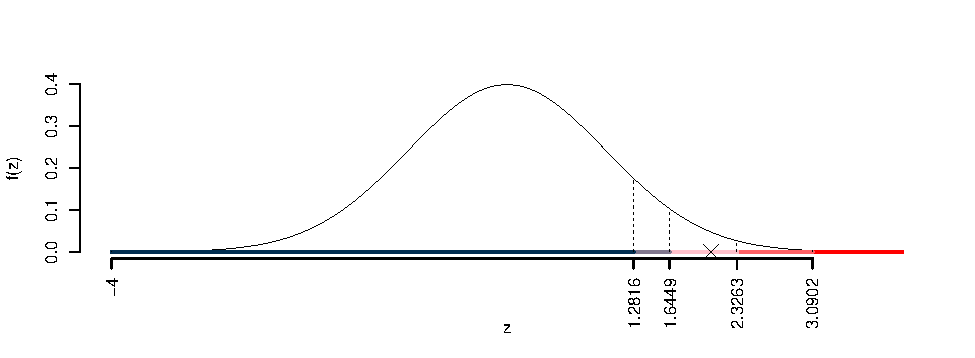
\includegraphics{Esami_passati_con_soluzioni_files/figure-latex/05-test-2,-1} \end{center}

Il \(p_{\text{value}}\) è

\[ p_{\text{value}} = P(Z>2.06)=0.019625 \]

\[
 0.01 < p_\text{value}= 0.019625 \leq 0.05 
\]

\end{sol}

\begin{center}\rule{0.5\linewidth}{0.5pt}\end{center}

2.a Un'indagine in 15 aziende, che producono lo stesso prodotto,
ha rilevato che il costo per unità è pari a euro 25.00
in media con una deviazione standard pari a euro 2.00.

Determinare un intervallo di confidenza al 95\%
per il costo medio per unità.

\begin{sol}
\(1-\alpha =0.95\) e quindi \(\alpha=0.05\rightarrow \alpha/2=0.025\)

\[
      S  =\sqrt{\frac {n}{n-1}}\cdot\hat\sigma =
     \sqrt{\frac { 15 }{ 14 }}\cdot 2 = 2.0702 
\]
\begin{eqnarray*}
  Idc: & &  \hat\mu \pm  t_{n-1;\alpha/2} \times \frac{S}{\sqrt{n}} \\
     & &  25 \pm  2.145 \times \frac{ 2.0702 }{\sqrt{ 15 }} \\
     & &  25 \pm  2.145 \times  0.5345 \\
     & & [ 23.85 ,  26.15 ]
\end{eqnarray*}

\end{sol}

2.b L'indagine dell'anno precedente, condotta
su un campione molto più numeroso, mostrava un costo medio
pari a euro 26.00 con una deviazione standard pari a 2.50 euro.
Verificare l'ipotesi che il costo medio del prodotto osservato
nell'anno corrente sia equivalente a quello osservato nell'anno
precedente contro l'alternativa di una diminuzione del costo.
Specificare in modo esplicito il tipo di test utilizzato,
l'ipotesi nulla e l'ipotesi alternativa e trarre le opportune
conclusioni.

\begin{sol}
\textbf{Test \(Z\) per una media, variazna nota}

\(\fbox{A}\) FORMULAZIONE DELLE IPOTESI

\[\begin{cases}
   H_0: \mu = \mu_0=26 \\
   H_1: \mu < \mu_0=26 
   \end{cases}\]

\(\fbox{B}\) SCELTA E CALCOLO STATISTICA-TEST, \(Z\)

\(\sigma^{2}\) di \(\cal{P}\) è nota: \(\Rightarrow\) z-Test.

\begin{eqnarray*}
   \frac{\hat\mu - \mu_{0}} {\sigma/\sqrt{n}}&\sim&N(0,1)\\
   z_{\text{obs}}
   &=& \frac{ ( 25 -  26 )} { 2.5 /\sqrt{ 15 }}
   =   -1.549 \, .
   \end{eqnarray*}

\(\fbox{C}\) CONCLUSIONE

Consideriamo \(\alpha=0.1, 0.05, 0.01, 0.001\)

I valori critici sono

\(z_{0.1}=-1.2816\); \(z_{0.05}=-1.6449\); \(z_{0.01}=-2.3263\); \(z_{0.001}=-3.0902\)

Siccome \(-3.0902<z_\text{obs}=-1.5492<-2.3263\), indecisione sul rifiuto di \(H_0\) al 10\%,

\(0.05<p_\text{value}<0.1\), \emph{marginalmente significativo} \(\fbox{.}\).

\begin{center}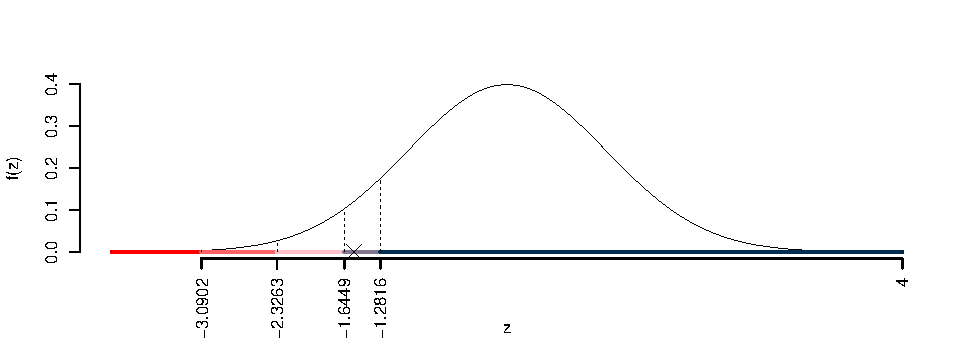
\includegraphics{Esami_passati_con_soluzioni_files/figure-latex/05-test-4,-1} \end{center}

Il \(p_{\text{value}}\) è

\[ p_{\text{value}} = P(Z<-1.55)=0.060668 \]

\[
 0.05 < p_\text{value}= 0.060668 \leq 0.1 
\]

\end{sol}

\begin{center}\rule{0.5\linewidth}{0.5pt}\end{center}

3.a Un'indagine in 20 aziende, che producono lo stesso prodotto,
ha rilevato che il costo per unità è pari a euro 28.00
in media con una deviazione standard pari a euro 1.80.

Determinare un intervallo di confidenza al 95\%
per il costo medio per unità.

\begin{sol}
\(1-\alpha =0.95\) e quindi \(\alpha=0.05\rightarrow \alpha/2=0.025\)

\[
      S  =\sqrt{\frac {n}{n-1}}\cdot\hat\sigma =
     \sqrt{\frac { 20 }{ 19 }}\cdot 1.8 = 1.8468 
\]
\begin{eqnarray*}
  Idc: & &  \hat\mu \pm  t_{n-1;\alpha/2} \times \frac{S}{\sqrt{n}} \\
     & &  28 \pm  2.093 \times \frac{ 1.8468 }{\sqrt{ 20 }} \\
     & &  28 \pm  2.093 \times  0.4129 \\
     & & [ 27.14 ,  28.86 ]
\end{eqnarray*}

\end{sol}

3.b L'indagine dell'anno precedente, condotta
su un campione molto più numeroso, mostrava un costo medio
pari a euro 27.00 con una deviazione standard pari a 2.20 euro.
Verificare l'ipotesi che il costo medio del prodotto osservato
nell'anno corrente sia equivalente a quello osservato nell'anno
precedente contro l'alternativa di un cambiamento del costo.
Specificare in modo esplicito il tipo di test utilizzato,
l'ipotesi nulla e l'ipotesi alternativa e trarre le opportune
conclusioni.

\begin{sol}
\textbf{Test \(Z\) per una media, variazna nota}

\(\fbox{A}\) FORMULAZIONE DELLE IPOTESI

\[\begin{cases}
   H_0: \mu = \mu_0=27 \\
   H_1: \mu \neq \mu_0=27 
   \end{cases}\]

\(\fbox{B}\) SCELTA E CALCOLO STATISTICA-TEST, \(Z\)

\(\sigma^{2}\) di \(\cal{P}\) è nota: \(\Rightarrow\) z-Test.

\begin{eqnarray*}
   \frac{\hat\mu - \mu_{0}} {\sigma/\sqrt{n}}&\sim&N(0,1)\\
   z_{\text{obs}}
   &=& \frac{ ( 28 -  27 )} { 2.2 /\sqrt{ 20 }}
   =   2.033 \, .
   \end{eqnarray*}

\(\fbox{C}\) CONCLUSIONE

Siccome \(H_1\) è bilaterale, considereremo \(\alpha/2\),
anziché \(\alpha\)

\(\alpha=0.1, 0.05, 0.01, 0.001\) e quindi \(\alpha/2=0.05, 0.025, 0.005, 0.0005\)

I valori critici sono

\(z_{0.05}=1.6449\); \(z_{0.025}=1.96\); \(z_{0.005}=2.5758\); \(z_{0.0005}=3.2905\)

Siccome \(1.96<|z_\text{obs}|=2.0328<2.5758\), quindi \textbf{rifiuto} \(H_0\) al 5\%,

\(0.01<p_\text{value}<0.05\), \emph{significativo} \(\fbox{*}\).

\begin{center}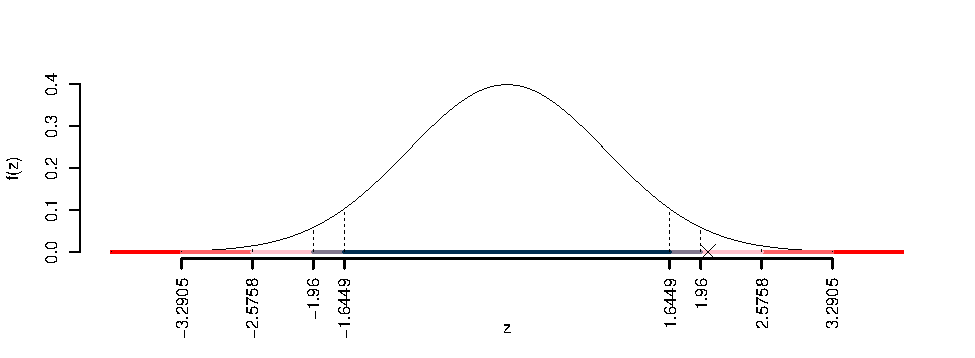
\includegraphics{Esami_passati_con_soluzioni_files/figure-latex/05-test-6,-1} \end{center}

Il \(p_{\text{value}}\) è

\[ p_{\text{value}} = P(|Z|>|2.03|)=2P(Z>2.03)=0.042074 \]

\[
 0.01 < p_\text{value}= 0.042074 \leq 0.05 
\]

\end{sol}

\section{\texorpdfstring{Un campione, IdC e test per \(\mu\), \(\sigma\) incognita (t test).}{Un campione, IdC e test per \textbackslash mu, \textbackslash sigma incognita (t test).}}\label{un-campione-idc-e-test-per-mu-sigma-incognita-t-test.}

4.a Sia \(X\) l'età dei parlamentari italiani.
Si sceglie un campione di 20 parlamentari italiani e si ottiene una
media di 48.5 anni con una deviazione standard pari a 10.6 anni.

Determinare un intervallo di confidenza al 95\% per
l'età media dei politici italiani.

\begin{sol}
\(1-\alpha =0.95\) e quindi \(\alpha=0.05\rightarrow \alpha/2=0.025\)

\[
      S  =\sqrt{\frac {n}{n-1}}\cdot\hat\sigma =
     \sqrt{\frac { 20 }{ 19 }}\cdot 10.6 = 10.8754 
\]
\begin{eqnarray*}
  Idc: & &  \hat\mu \pm  t_{n-1;\alpha/2} \times \frac{S}{\sqrt{n}} \\
     & &  48.5 \pm  2.093 \times \frac{ 10.8754 }{\sqrt{ 20 }} \\
     & &  48.5 \pm  2.093 \times  2.432 \\
     & & [ 43.41 ,  53.59 ]
\end{eqnarray*}

\end{sol}

4.b è noto che l'età media dei politici europei
è di 55 anni.
Verificare l'ipotesi
che l'età media dei politici italiani sia uguale a quella
dei politici europei contro l'alternativa che sia minore.
Specificare in modo esplicito il tipo di test utilizzato,
l'ipotesi nulla e l'ipotesi alternativa e trarre le opportune
conclusioni.

\begin{sol}
\textbf{Test \(t\) per una media, varianza incognita}

\(\fbox{A}\) FORMULAZIONE DELLE IPOTESI

\[\begin{cases}
   H_0: \mu = \mu_0=55 \\
   H_1: \mu < \mu_0=55 
   \end{cases}\]

\begin{eqnarray*}
   S    &=& \sqrt{\frac{n} {n-1}}\ \widehat{\sigma} 
   =  \sqrt{\frac{ 20 } { 20 -1}} \times  10.6  =  10.88 
   \end{eqnarray*}
\begin{eqnarray*}
   \frac{\hat\mu - \mu_{0}} {S/\,\sqrt{n}}&\sim&t_{n-1}\\
   t_{\text{obs}}
   &=& \frac{ ( 48.5 -  55 )} { 10.88 /\sqrt{ 20 }}
   =   -2.673 \, .
   \end{eqnarray*}

\(\fbox{C}\) CONCLUSIONE

Consideriamo \(\alpha=0.1, 0.05, 0.01, 0.001\)

I valori critici sono

\(t_{20-1;0.1}=-1.3277\); \(t_{20-1;0.05}=-1.7291\); \(t_{20-1;0.01}=-2.5395\); \(t_{20-1;0.001}=-3.5794\)

Siccome \(-1.7291<t_\text{obs}=-2.6729<-1.3277\), quindi \textbf{rifiuto} \(H_0\) all'1\%,

\(0.001<p_\text{value}<0.01\), \emph{molto significativo} \(\fbox{**}\).

\begin{center}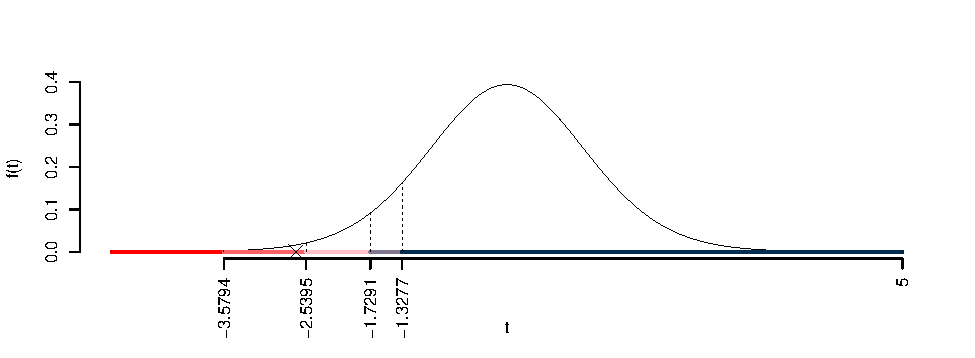
\includegraphics{Esami_passati_con_soluzioni_files/figure-latex/05-test-8,-1} \end{center}

Il \(p_{\text{value}}\) è

\[ p_{\text{value}} = P(T_{20-1}<-2.67)=0.007521 \]

Attenzione il calcolo del \(p_\text{value}\) con la \(T\) è puramente illustrativo e non può essere riprodotto senza una calcolatrice statistica adeguata.\[
 0.001 < p_\text{value}= 0.007521 \leq 0.01 
\]

\end{sol}

\begin{center}\rule{0.5\linewidth}{0.5pt}\end{center}

5.a Sia \(X\) il reddito annuale dei manager italiani.
Si sceglie un campione di 30 manager italiani e si ottiene una
media di 85 mila euro con una deviazione standard pari a 15 mila euro.

Determinare un intervallo di confidenza al 99\% per
il reddito medio annuale dei manager italiani.

\begin{sol}
\(1-\alpha =0.99\) e quindi \(\alpha=0.01\rightarrow \alpha/2=0.005\)

\[
      S  =\sqrt{\frac {n}{n-1}}\cdot\hat\sigma =
     \sqrt{\frac { 30 }{ 29 }}\cdot 15 = 15.2564 
\]
\begin{eqnarray*}
  Idc: & &  \hat\mu \pm  t_{n-1;\alpha/2} \times \frac{S}{\sqrt{n}} \\
     & &  85 \pm  2.756 \times \frac{ 15.2564 }{\sqrt{ 30 }} \\
     & &  85 \pm  2.756 \times  2.785 \\
     & & [ 77.32 ,  92.68 ]
\end{eqnarray*}

\end{sol}

5.b è noto che il reddito medio annuale dei manager europei
è di 80 mila euro.
Verificare l'ipotesi
che il reddito medio annuale dei manager italiani sia uguale a quello
dei manager europei contro l'alternativa che sia maggiore.
Specificare in modo esplicito il tipo di test utilizzato,
l'ipotesi nulla e l'ipotesi alternativa e trarre le opportune
conclusioni.

\begin{sol}
\textbf{Test \(t\) per una media, varianza incognita}

\(\fbox{A}\) FORMULAZIONE DELLE IPOTESI

\[\begin{cases}
   H_0: \mu = \mu_0=80 \\
   H_1: \mu > \mu_0=80 
   \end{cases}\]

\begin{eqnarray*}
   S    &=& \sqrt{\frac{n} {n-1}}\ \widehat{\sigma} 
   =  \sqrt{\frac{ 30 } { 30 -1}} \times  15  =  15.26 
   \end{eqnarray*}
\begin{eqnarray*}
   \frac{\hat\mu - \mu_{0}} {S/\,\sqrt{n}}&\sim&t_{n-1}\\
   t_{\text{obs}}
   &=& \frac{ ( 85 -  80 )} { 15.26 /\sqrt{ 30 }}
   =   1.795 \, .
   \end{eqnarray*}

\(\fbox{C}\) CONCLUSIONE

Consideriamo \(\alpha=0.1, 0.05, 0.01, 0.001\)

I valori critici sono

\(t_{30-1;0.1}=1.3114\); \(t_{30-1;0.05}=1.6991\); \(t_{30-1;0.01}=2.462\); \(t_{30-1;0.001}=3.3962\)

Siccome \(1.6991<t_\text{obs}=1.7951<2.462\), quindi \textbf{rifiuto} \(H_0\) al 5\%,

\(0.01<p_\text{value}<0.05\), \emph{significativo} \(\fbox{*}\).

\begin{center}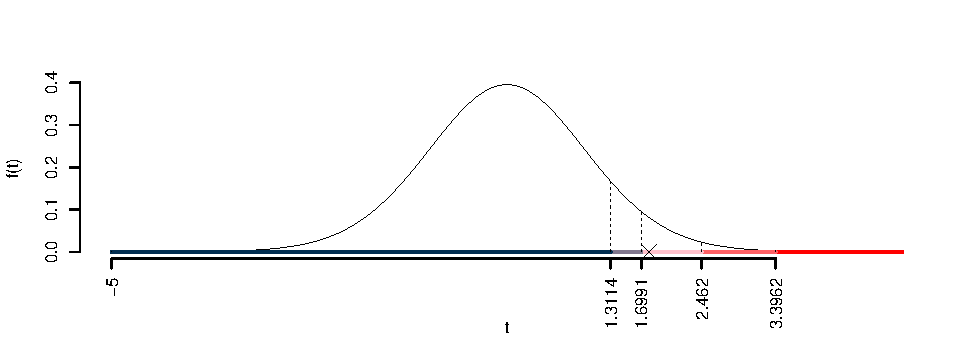
\includegraphics{Esami_passati_con_soluzioni_files/figure-latex/05-test-10,-1} \end{center}

Il \(p_{\text{value}}\) è

\[ p_{\text{value}} = P(T_{30-1}>1.8)=0.041537 \]

Attenzione il calcolo del \(p_\text{value}\) con la \(T\) è puramente illustrativo e non può essere riprodotto senza una calcolatrice statistica adeguata.\[
 0.01 < p_\text{value}= 0.041537 \leq 0.05 
\]

\end{sol}

\begin{center}\rule{0.5\linewidth}{0.5pt}\end{center}

6.a Per accertare lo stato di preparazione dei dipendenti di una
struttura pubblica si è estratto un campione di 26 impiegati.
A ogni impiegato è stato somministrato un test, con
punteggio da 0 a 100, per accertare il suo grado di competenza, \(X\).
Il valore medio ottenuto è pari a 78 con una deviazione
standard pari a 12.

Determinare un intervallo di confidenza
al 95\% per \(\mu = E(X)\).

\begin{sol}
\(1-\alpha =0.95\) e quindi \(\alpha=0.05\rightarrow \alpha/2=0.025\)

\[
      S  =\sqrt{\frac {n}{n-1}}\cdot\hat\sigma =
     \sqrt{\frac { 26 }{ 25 }}\cdot 12 = 12.2376 
\]
\begin{eqnarray*}
  Idc: & &  \hat\mu \pm  t_{n-1;\alpha/2} \times \frac{S}{\sqrt{n}} \\
     & &  78 \pm  2.06 \times \frac{ 12.2376 }{\sqrt{ 26 }} \\
     & &  78 \pm  2.06 \times  2.4 \\
     & & [ 73.06 ,  82.94 ]
\end{eqnarray*}

\end{sol}

6.b Si supponga che il punteggio medio del test in un ampio
studio sulla popolazione di impiegati, sia pari a 72.
Con un livello di significatività uguale a 0.01 si può
ritenere che il valore medio osservato nel campione sia
diverso da 72?

\begin{sol}
\textbf{Test \(t\) per una media, varianza incognita}

\(\fbox{A}\) FORMULAZIONE DELLE IPOTESI

\[\begin{cases}
   H_0: \mu = \mu_0=72 \\
   H_1: \mu \neq \mu_0=72 
   \end{cases}\]

\begin{eqnarray*}
   S    &=& \sqrt{\frac{n} {n-1}}\ \widehat{\sigma} 
   =  \sqrt{\frac{ 26 } { 26 -1}} \times  12  =  12.24 
   \end{eqnarray*}
\begin{eqnarray*}
   \frac{\hat\mu - \mu_{0}} {S/\,\sqrt{n}}&\sim&t_{n-1}\\
   t_{\text{obs}}
   &=& \frac{ ( 78 -  72 )} { 12.24 /\sqrt{ 26 }}
   =   2.5 \, .
   \end{eqnarray*}

\(\fbox{C}\) CONCLUSIONE

Siccome \(H_1\) è bilaterale, considereremo \(\alpha/2\),
anziché \(\alpha\)

\(\alpha=0.1, 0.05, 0.01, 0.001\) e quindi \(\alpha/2=0.05, 0.025, 0.005, 0.0005\)

I valori critici sono

\(t_{26-1;0.05}=1.7081\); \(t_{26-1;0.025}=2.0595\); \(t_{26-1;0.005}=2.7874\); \(t_{26-1;0.0005}=3.7251\)

Siccome \(2.0595<|t_\text{obs}|=2.5<2.7874\), quindi \textbf{rifiuto} \(H_0\) al 5\%,

\(0.01<p_\text{value}<0.05\), \emph{significativo} \(\fbox{*}\).

\begin{center}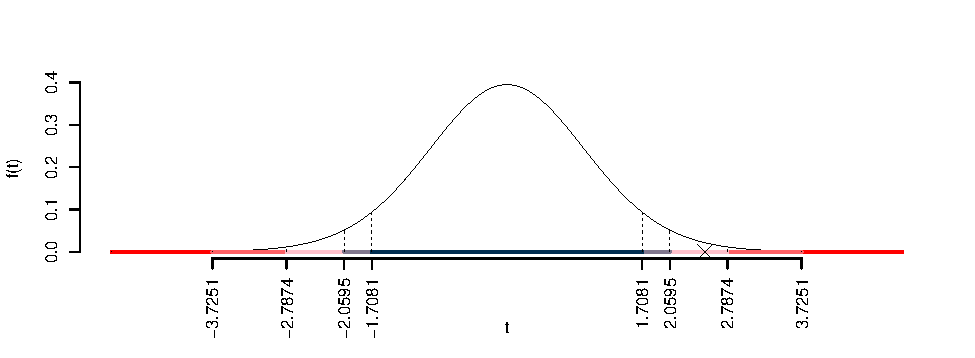
\includegraphics{Esami_passati_con_soluzioni_files/figure-latex/05-test-12,-1} \end{center}

Il \(p_{\text{value}}\) è

\[ p_{\text{value}} = P(|T_{26-1}|>|2.5|)=2P(T_{26-1}>2.5)=0.019343 \]

Attenzione il calcolo del \(p_\text{value}\) con la \(T\) è puramente illustrativo e non può essere riprodotto senza una calcolatrice statistica adeguata.\[
 0.01 < p_\text{value}= 0.019343 \leq 0.05 
\]

\end{sol}

\section{\texorpdfstring{Un campione, IdC e test per \(\pi\) (z test).}{Un campione, IdC e test per \textbackslash pi (z test).}}\label{un-campione-idc-e-test-per-pi-z-test.}

7.a Su un campione di \(n = 100\) abitanti del quartiere \emph{R} è stato chiesto se siano favorevoli o meno all'introduzione di una nuova pista ciclabile. Lo studio ha riportato che 70 persone su 100 (il 70\% del campione) è favorevole.

Costruire un intervallo di confidenza al 95\% per \(\pi\) la quota di persone del quartiere \emph{R} favorevole alla nuova pista ciclabile.

\begin{sol}
\(1-\alpha =0.95\) e quindi \(\alpha=0.05\rightarrow \alpha/2=0.025\)

\[
  \hat\pi = \frac{S_n}n = \frac{ 70 }{ 100 }= 0.7 
\]

\begin{eqnarray*}
  Idc: & &  \hat\pi \pm  z_{\alpha/2} \times \sqrt{\frac{\hat\pi(1-\hat\pi)}{n}} \\
     & &  0.7 \pm  1.96 \times \sqrt{\frac{ 0.7 (1- 0.7 )}{ 100 }} \\
     & &  0.7 \pm  1.96 \times  0.04583 \\
     & & [ 0.6102 ,  0.7898 ]
\end{eqnarray*}

\end{sol}

7.b Un'indagine molto più ampia condotta su tutta la città ha mostrato che
la percentuale di favorevoli alla pista ciclabile è del 65\%. Testare l'ipotesi che nel quartiere \emph{R} la quota di favorevoli sia uguale a quella cittadina contro l'alternativa che sia minore.

\begin{sol}
\textbf{Test \(Z\) per una proporzione}

La stima
\[\hat\pi=\frac { 70 } { 100 }= 0.7  \]

\(\fbox{A}\) FORMULAZIONE DELLE IPOTESI

\[\begin{cases}
   H_0: \pi = \pi_0=0.65 \\
   H_1: \pi > \pi_0=0.65 
   \end{cases}\]

\(\fbox{B}\) SCELTA E CALCOLO STATISTICA-TEST, \(Z\)
Test Binomiale per \(n\) grande: \(\Rightarrow\) z-Test.

\begin{eqnarray*}
   \frac{\hat\pi - \pi_{0}} {\sqrt {\pi_0(1-\pi_0)/\,n}}&\sim&N(0,1)\\
   z_{\text{obs}}
   &=& \frac{ ( 0.7 -  0.65 )} {\sqrt{ 0.65 (1- 0.65 )/ 100 }}
   =   1.048 \,.
   \end{eqnarray*}

\(\fbox{C}\) CONCLUSIONE

Il \(p_{\text{value}}\) è

\[ p_{\text{value}} = P(Z>1.05)=0.147254 \]

\[
 0.1 < p_\text{value}= 0.147254 \leq 1 
\]

\begin{center}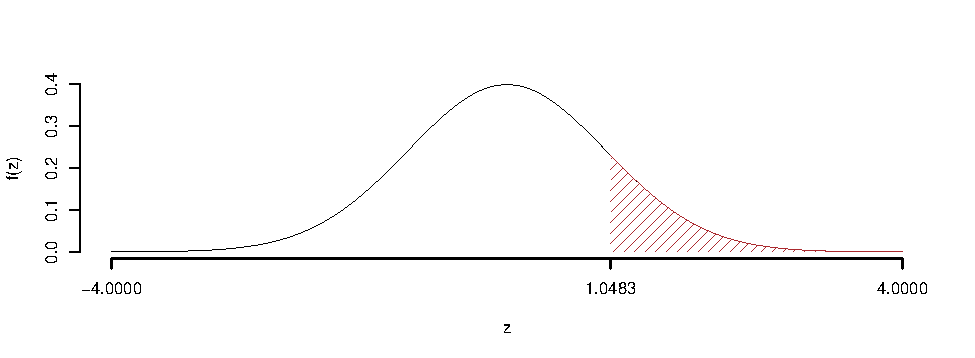
\includegraphics{Esami_passati_con_soluzioni_files/figure-latex/05-test-21-1} \end{center}

\textbf{Non} rifiuto \(H_0\) a \textbf{nessun}
livello di significatività,

\(p_\text{value}>0.1\),
\emph{non significativo}

\end{sol}

\begin{center}\rule{0.5\linewidth}{0.5pt}\end{center}

8.a Su un campione di \(n = 120\) startup tecnologiche italiane, è stato chiesto se abbiano implementato misure di cybersecurity avanzate. Lo studio ha riportato che 84 startup su 120 (il 70\% del campione) hanno implementato queste misure.

Costruire un intervallo di confidenza al 99\% per \(\pi\), la quota di startup italiane che hanno implementato misure di cybersecurity avanzate.

\begin{sol}
\(1-\alpha =0.99\) e quindi \(\alpha=0.01\rightarrow \alpha/2=0.005\)

\[
  \hat\pi = \frac{S_n}n = \frac{ 84 }{ 120 }= 0.7 
\]

\begin{eqnarray*}
  Idc: & &  \hat\pi \pm  z_{\alpha/2} \times \sqrt{\frac{\hat\pi(1-\hat\pi)}{n}} \\
     & &  0.7 \pm  2.576 \times \sqrt{\frac{ 0.7 (1- 0.7 )}{ 120 }} \\
     & &  0.7 \pm  2.576 \times  0.04183 \\
     & & [ 0.5922 ,  0.8078 ]
\end{eqnarray*}

\end{sol}

8.b Un'indagine molto più ampia condotta su startup europee ha mostrato che la percentuale di startup con misure di cybersecurity avanzate è del 75\%. Testare l'ipotesi che in Italia la quota di startup con misure di cybersecurity avanzate sia uguale a quella europea contro l'alternativa che sia diversa.

\begin{sol}
\textbf{Test \(Z\) per una proporzione}

La stima
\[\hat\pi=\frac { 84 } { 120 }= 0.7  \]

\(\fbox{A}\) FORMULAZIONE DELLE IPOTESI

\[\begin{cases}
   H_0: \pi = \pi_0=0.75 \\
   H_1: \pi \neq \pi_0=0.75 
   \end{cases}\]

\(\fbox{B}\) SCELTA E CALCOLO STATISTICA-TEST, \(Z\)
Test Binomiale per \(n\) grande: \(\Rightarrow\) z-Test.

\begin{eqnarray*}
   \frac{\hat\pi - \pi_{0}} {\sqrt {\pi_0(1-\pi_0)/\,n}}&\sim&N(0,1)\\
   z_{\text{obs}}
   &=& \frac{ ( 0.7 -  0.75 )} {\sqrt{ 0.75 (1- 0.75 )/ 120 }}
   =   -1.265 \,.
   \end{eqnarray*}

\(\fbox{C}\) CONCLUSIONE

Il \(p_{\text{value}}\) è

\[ p_{\text{value}} = P(|Z|>|-1.26|)=2P(Z>1.26)=0.205903 \]

\[
 0.1 < p_\text{value}= 0.205903 \leq 1 
\]

\begin{center}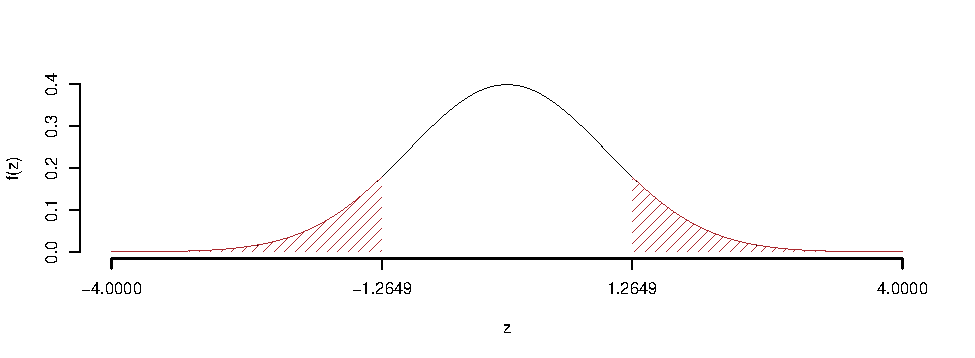
\includegraphics{Esami_passati_con_soluzioni_files/figure-latex/05-test-23-1} \end{center}

\textbf{Non} rifiuto \(H_0\) a \textbf{nessun}
livello di significatività,

\(p_\text{value}>0.1\),
\emph{non significativo}

\end{sol}

\section{t-Test a due campioni}\label{t-test-a-due-campioni}

9.a In uno studio sull'efficacia della pubblicità
si è proceduto facendo vedere lo spot \(A\) ad un campione di 10
individui (gruppo \(A\)) e lo spot \(B\) ad un secondo campione di 20
individui (gruppo \(B\)).
Si è quindi misurato il gradimento con opportuna scala.
Il gradimento medio del gruppo \(A\) risulta pari a 95 con una
deviazione standard pari a 1.9 mentre il gradimento medio del
gruppo \(B\) risulta pari a 92 con una deviazione standard pari
a 3.4.
Verificare l'ipotesi che il gradimento medio dei due spot sia uguale, contro
l'alternativa che lo spot \(A\) sia mediamente più gradito
di quello \(B\).
Si assuma l'ipotesi di eterogeneità delle varianze dei due
gruppi.

\begin{sol}
\textbf{Test \(t\) per due medie, (eterogeneità)}

\(\fbox{A}\) FORMULAZIONE DELLE IPOTESI

\[\begin{cases}
   H_0: \mu_\text{A} = \mu_\text{B} \\
   H_1: \mu_\text{A} > \mu_\text{B} 
   \end{cases}\]

\(\fbox{B}\) SCELTA E CALCOLO STATISTICA-TEST, \(T\)
\[
     S^2_\text{ A }=\frac{n_\text{ A }}{n_\text{ A }-1}\hat\sigma^2_\text{ A }=\frac{ 10 }{ 10 -1} 3.4 ^2= 12.84  \qquad
     S^2_\text{ B }=\frac{n_\text{ B }}{n_\text{ B }-1}\hat\sigma^2_\text{ B }=\frac{ 20 }{ 20 -1} 1.9 ^2= 3.8 
   \]

\begin{eqnarray*}
   \frac{\hat\mu_\text{ A } - \hat\mu_\text{ B }}
   {\sqrt{\frac {S^2_\text{ A }}{n_\text{ A }}+\frac {S^2_\text{ B }}{n_\text{ B }}}}&\sim&t_{n_\text{ A }+n_\text{ B }-2}\\
   t_{\text{obs}}
   &=& \frac{ ( 95 -  92 )} {\sqrt{\frac{ 12.84 }{ 10 }+\frac{ 3.8 }{ 20 }}}
   =   2.471 \, .
   \end{eqnarray*}

\(\fbox{C}\) CONCLUSIONE

Consideriamo \(\alpha=0.1, 0.05, 0.01, 0.001\)

I valori critici sono

\(t_{30-2;0.1}=1.3125\); \(t_{30-2;0.05}=1.7011\); \(t_{30-2;0.01}=2.4671\); \(t_{30-2;0.001}=3.4082\)

Siccome \(2.4671<t_\text{obs}=2.4706<3.4082\), quindi \textbf{rifiuto} \(H_0\) all'1\%,

\(0.001<p_\text{value}<0.01\), \emph{molto significativo} \(\fbox{**}\).

\begin{center}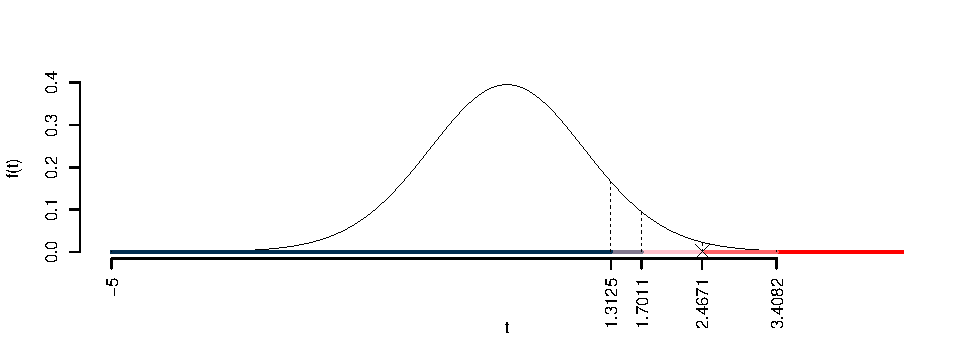
\includegraphics{Esami_passati_con_soluzioni_files/figure-latex/05-test-13,-1} \end{center}

Il \(p_{\text{value}}\) è

\[ p_{\text{value}} = P(T_{30-2}>2.47)=0.009921 \]

Attenzione il calcolo del \(p_\text{value}\) con la \(T\) è puramente illustrativo e non può essere riprodotto senza una calcolatrice statistica adeguata.\[
 0.001 < p_\text{value}= 0.009921 \leq 0.01 
\]

\end{sol}

\begin{center}\rule{0.5\linewidth}{0.5pt}\end{center}

10.a In uno studio sull'efficacia di due metodi di insegnamento della matematica, si è proceduto facendo seguire il metodo \(A\) ad un campione di 15 studenti (gruppo \(A\)) e il metodo \(B\) ad un secondo campione di 18 studenti (gruppo \(B\)). Si è quindi misurata la prestazione degli studenti con un test finale. La prestazione media del gruppo \(A\) risulta pari a 78 con una deviazione standard pari a 8.3, mentre la prestazione media del gruppo \(B\) risulta pari a 74 con una deviazione standard pari a 7.5. Verificare l'ipotesi che la prestazione media dei due metodi di insegnamento sia uguale, contro l'alternativa che il metodo \(A\) produca prestazioni mediamente migliori di quello \(B\). Si assuma l'ipotesi di eterogeneità delle varianze dei due gruppi, anche se i numeri non sembrano giustificarla.

\begin{sol}
\textbf{Test \(t\) per due medie, (eterogeneità)}

\(\fbox{A}\) FORMULAZIONE DELLE IPOTESI

\[\begin{cases}
   H_0: \mu_\text{A} = \mu_\text{B} \\
   H_1: \mu_\text{A} > \mu_\text{B} 
   \end{cases}\]

\(\fbox{B}\) SCELTA E CALCOLO STATISTICA-TEST, \(T\)
\[
     S^2_\text{ A }=\frac{n_\text{ A }}{n_\text{ A }-1}\hat\sigma^2_\text{ A }=\frac{ 15 }{ 15 -1} 8.3 ^2= 73.81  \qquad
     S^2_\text{ B }=\frac{n_\text{ B }}{n_\text{ B }-1}\hat\sigma^2_\text{ B }=\frac{ 18 }{ 18 -1} 7.5 ^2= 59.56 
   \]

\begin{eqnarray*}
   \frac{\hat\mu_\text{ A } - \hat\mu_\text{ B }}
   {\sqrt{\frac {S^2_\text{ A }}{n_\text{ A }}+\frac {S^2_\text{ B }}{n_\text{ B }}}}&\sim&t_{n_\text{ A }+n_\text{ B }-2}\\
   t_{\text{obs}}
   &=& \frac{ ( 78 -  74 )} {\sqrt{\frac{ 73.81 }{ 15 }+\frac{ 59.56 }{ 18 }}}
   =   1.394 \, .
   \end{eqnarray*}

\(\fbox{C}\) CONCLUSIONE

Consideriamo \(\alpha=0.1, 0.05, 0.01, 0.001\)

I valori critici sono

\(t_{33-2;0.1}=1.3095\); \(t_{33-2;0.05}=1.6955\); \(t_{33-2;0.01}=2.4528\); \(t_{33-2;0.001}=3.3749\)

Siccome \(1.3095<t_\text{obs}=1.3944<1.6955\), indecisione sul rifiuto di \(H_0\) al 10\%,

\(0.05<p_\text{value}<0.1\), \emph{marginalmente significativo} \(\fbox{.}\).

\begin{center}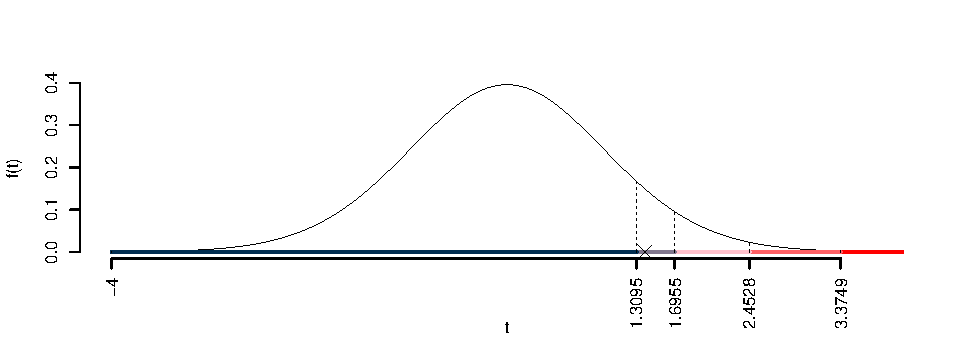
\includegraphics{Esami_passati_con_soluzioni_files/figure-latex/05-test-14,-1} \end{center}

Il \(p_{\text{value}}\) è

\[ p_{\text{value}} = P(T_{33-2}>1.39)=0.086563 \]

Attenzione il calcolo del \(p_\text{value}\) con la \(T\) è puramente illustrativo e non può essere riprodotto senza una calcolatrice statistica adeguata.\[
 0.05 < p_\text{value}= 0.086563 \leq 0.1 
\]

\end{sol}

\begin{center}\rule{0.5\linewidth}{0.5pt}\end{center}

11.a In uno studio sulla produttività dei lavoratori, si è proceduto confrontando 15 lavoratori del Nord e 18 del Sud. Si è quindi misurata la produttività media con un'opportuna scala. La produttività media del gruppo Nord risulta pari a 85 con una deviazione standard pari a 7.2, mentre la produttività media del gruppo Sud risulta pari a 80 con una deviazione standard pari a 6.8. Verificare l'ipotesi che la produttività media dei due gruppi sia uguale, contro l'alternativa che le due produttività medie siano diverse. Si assuma l'ipotesi di omogeneità delle varianze dei due gruppi.

\begin{sol}
\textbf{Test \(T\) per due medie, (omogeneità)}

\(\fbox{A}\) FORMULAZIONE DELLE IPOTESI

\[\begin{cases}
   H_0: \mu_\text{Nord} = \mu_\text{Sud} \\
   H_1: \mu_\text{Nord} \neq \mu_\text{Sud} 
   \end{cases}\]

\(\fbox{B}\) SCELTA E CALCOLO STATISTICA-TEST, \(T\)

L'ipotesi è di omogeneità e quindi calcoliamo:\[
   S_p^2=\frac{n_\text{ Nord }\hat\sigma^2_\text{ Nord }+n_\text{ Sud }\hat\sigma^2_\text{ Sud }}{n_\text{ Nord }+n_\text{ Sud }-2} =
   \frac{ 15 \cdot 7.2 ^2+ 18 \cdot 6.8 ^2}{ 15 + 18 -2}= 51.93 
  \]

\begin{eqnarray*}
  \frac{\hat\mu_\text{ Nord } - \hat\mu_\text{ Sud }}
  {\sqrt{\frac {S^2_p}{n_\text{ Nord }}+\frac {S^2_p}{n_\text{ Sud }}}}&\sim&t_{n_\text{ Nord }+n_\text{ Sud }-2}\\
  t_{\text{obs}}
  &=& \frac{ ( 85 -  80 )} {\sqrt{\frac{ 51.93 }{ 15 }+\frac{ 51.93 }{ 18 }}}
  =   1.985 \, .
  \end{eqnarray*}

\(\fbox{C}\) CONCLUSIONE

Siccome \(H_1\) è bilaterale, considereremo \(\alpha/2\),
anziché \(\alpha\)

\(\alpha=0.1, 0.05, 0.01, 0.001\) e quindi \(\alpha/2=0.05, 0.025, 0.005, 0.0005\)

I valori critici sono

\(t_{33-2;0.05}=1.6955\); \(t_{33-2;0.025}=2.0395\); \(t_{33-2;0.005}=2.744\); \(t_{33-2;0.0005}=3.6335\)

Siccome \(1.6955<|t_\text{obs}|=1.9846<2.0395\), indecisione sul rifiuto di \(H_0\) al 10\%,

\(0.05<p_\text{value}<0.1\), \emph{marginalmente significativo} \(\fbox{.}\).

\begin{center}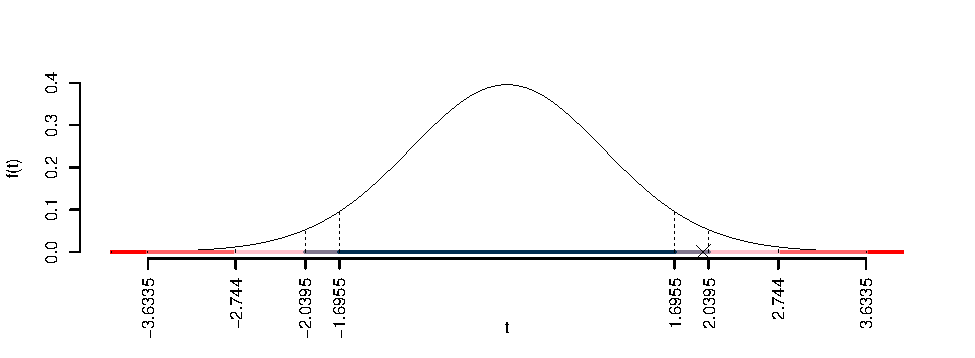
\includegraphics{Esami_passati_con_soluzioni_files/figure-latex/05-test-15,-1} \end{center}

Il \(p_{\text{value}}\) è

\[ p_{\text{value}} = P(|T_{33-2}|>|1.98|)=2P(T_{33-2}>1.98)=0.056100 \]

Attenzione il calcolo del \(p_\text{value}\) con la \(T\) è puramente illustrativo e non può essere riprodotto senza una calcolatrice statistica adeguata.\[
 0.05 < p_\text{value}= 0.056100 \leq 0.1 
\]

\end{sol}

\section{Due campioni: proporzione}\label{due-campioni-proporzione}

12.a Per verificare se ci sia differenza di genere sulla
riforma costituzionale del governo Meloni, si è condotta una
indagine su 120 donne e 120 uomini.
Dalle interviste è emerso che 60 dei 120 uomini si siano
dichiarati favorevoli, mentre 30 delle 120 donne si siano
dichiarate favorevoli (numeri di comodo per avere pochi decimali).
Verificare l'ipotesi
che non ci sia differenza tra uomini e donne, contro l'alternativa
che le donne siano meno favorevoli alla riforma costituzionale.
Specificare l'ipotesi nulla e l'ipotesi alternativa,
il tipo di test da utilizzare, e le conclusioni.

\begin{sol}
\textbf{Test \(Z\) per due proporzioni}

\(\fbox{A}\) FORMULAZIONE DELLE IPOTESI

\[\begin{cases}
   H_0: \pi_\text{U} = \pi_\text{D} \\
   H_1: \pi_\text{U} > \pi_\text{D} 
   \end{cases}\]

\(\fbox{B}\) SCELTA E CALCOLO STATISTICA-TEST, \(Z\)

\[\hat\pi_\text{ U }=\frac{s_\text{ U }}{n_\text{ U }}=\frac{ 60 }{ 120 }= 0.5 \qquad
   \hat\pi_\text{ D }=\frac{s_\text{ D }}{n_\text{ D }}=\frac{ 30 }{ 120 }= 0.25 \]Calcoliamo la proporzione comune sotto \(H_0\)
\[
     \pi_C=\frac{s_\text{ U }+s_\text{ D }}{n_\text{ U }+n_\text{ D }}=
     \frac{ 90 }{ 240 }= 0.375 
   \]\begin{eqnarray*}
   \frac{\hat\pi_\text{ U } - \hat\pi_\text{ D }}
   {\sqrt{\frac {\pi_C(1-\pi_C)}{n_\text{ U }}+\frac {\pi_C(1-\pi_C)}{n_\text{ D }}}}&\sim&N(0,1)\\
   z_{\text{obs}}
   &=& \frac{ ( 0.5 -  0.25 )} {\sqrt{\frac{ 0.375 (1- 0.375 )}{ 120 }+\frac{ 0.375 (1- 0.375 )}{ 120 }}}
   =   4 \, .
   \end{eqnarray*}

\(\fbox{C}\) CONCLUSIONE

Il \(p_{\text{value}}\) è

\[ p_{\text{value}} = P(Z>4)=0.000032 \]

\[
 0 < p_\text{value}= 0.000032 \leq 0.001 
\]

\begin{center}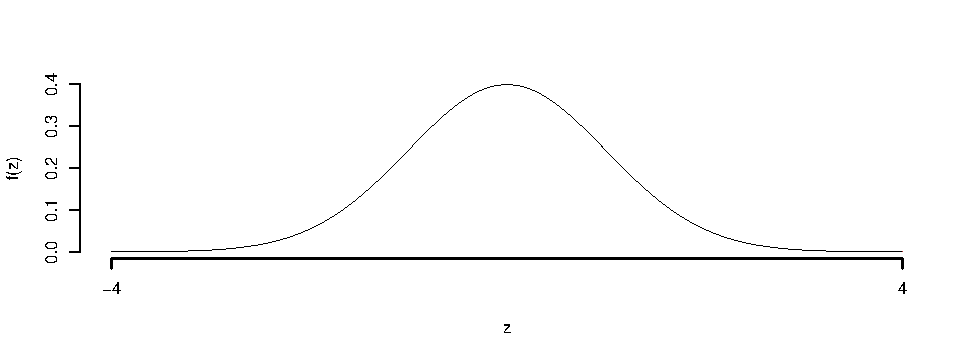
\includegraphics{Esami_passati_con_soluzioni_files/figure-latex/05-test-16,-1} \end{center}

\textbf{Rifiuto} \(H_0\) sotto all'1‰,

\(p_\text{value}<0.001\), \emph{estremamente significativo} \(\fbox{***}\).

\end{sol}

\begin{center}\rule{0.5\linewidth}{0.5pt}\end{center}

13.a Per verificare se ci sia differenza nella soddisfazione lavorativa tra dipendenti a tempo pieno e part-time, si è condotta un'indagine su 100 dipendenti a tempo pieno e 100 dipendenti part-time. Dalle interviste è emerso che 70 dei 100 dipendenti a tempo pieno si siano dichiarati soddisfatti, mentre 50 dei 100 dipendenti part-time si siano dichiarati soddisfatti. Verificare l'ipotesi che non ci sia differenza nella soddisfazione lavorativa tra dipendenti a tempo pieno e part-time, contro l'alternativa che i dipendenti part-time siano meno soddisfatti. Specificare l'ipotesi nulla e l'ipotesi alternativa, il tipo di test da utilizzare, e le conclusioni.

\begin{sol}
\textbf{Test \(Z\) per due proporzioni}

\(\fbox{A}\) FORMULAZIONE DELLE IPOTESI

\[\begin{cases}
   H_0: \pi_\text{Tempo Pieno} = \pi_\text{Part-Time} \\
   H_1: \pi_\text{Tempo Pieno} > \pi_\text{Part-Time} 
   \end{cases}\]

\(\fbox{B}\) SCELTA E CALCOLO STATISTICA-TEST, \(Z\)

\[\hat\pi_\text{ Tempo Pieno }=\frac{s_\text{ Tempo Pieno }}{n_\text{ Tempo Pieno }}=\frac{ 70 }{ 100 }= 0.7 \qquad
   \hat\pi_\text{ Part-Time }=\frac{s_\text{ Part-Time }}{n_\text{ Part-Time }}=\frac{ 50 }{ 100 }= 0.5 \]Calcoliamo la proporzione comune sotto \(H_0\)
\[
     \pi_C=\frac{s_\text{ Tempo Pieno }+s_\text{ Part-Time }}{n_\text{ Tempo Pieno }+n_\text{ Part-Time }}=
     \frac{ 120 }{ 200 }= 0.6 
   \]\begin{eqnarray*}
   \frac{\hat\pi_\text{ Tempo Pieno } - \hat\pi_\text{ Part-Time }}
   {\sqrt{\frac {\pi_C(1-\pi_C)}{n_\text{ Tempo Pieno }}+\frac {\pi_C(1-\pi_C)}{n_\text{ Part-Time }}}}&\sim&N(0,1)\\
   z_{\text{obs}}
   &=& \frac{ ( 0.7 -  0.5 )} {\sqrt{\frac{ 0.6 (1- 0.6 )}{ 100 }+\frac{ 0.6 (1- 0.6 )}{ 100 }}}
   =   2.887 \, .
   \end{eqnarray*}

\(\fbox{C}\) CONCLUSIONE

Il \(p_{\text{value}}\) è

\[ p_{\text{value}} = P(Z>2.89)=0.001946 \]

\[
 0.001 < p_\text{value}= 0.001946 \leq 0.01 
\]

\begin{center}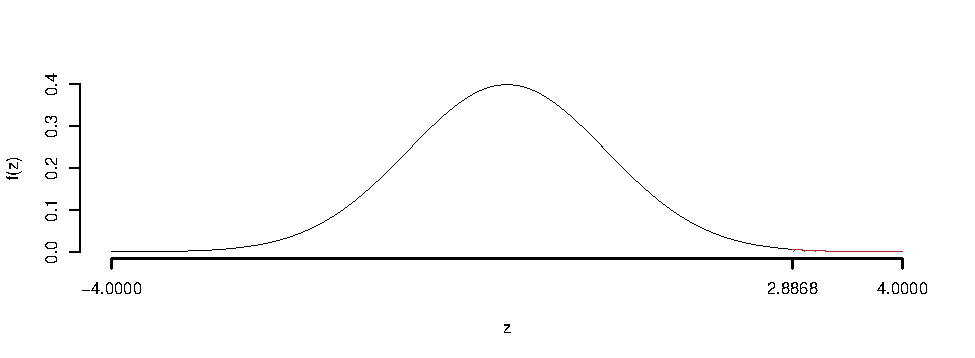
\includegraphics{Esami_passati_con_soluzioni_files/figure-latex/05-test-17,-1} \end{center}

\textbf{Rifiuto} \(H_0\) all'1\%,

\(0.001<p_\text{value}<0.01\), \emph{molto significativo} \(\fbox{**}\).

\end{sol}

\begin{center}\rule{0.5\linewidth}{0.5pt}\end{center}

14.a Per verificare se ci sia differenza nella preferenza per il lavoro remoto tra dipendenti di aziende tecnologiche e dipendenti di aziende manifatturiere, si è condotta un'indagine su 90 dipendenti di aziende tecnologiche e 90 dipendenti di aziende manifatturiere. Dalle interviste è emerso che 63 dei 90 dipendenti di aziende tecnologiche preferiscono il lavoro remoto, mentre 45 dei 90 dipendenti di aziende manifatturiere preferiscono il lavoro remoto. Verificare l'ipotesi che non ci sia differenza nella preferenza per il lavoro remoto tra i due gruppi, contro l'alternativa che ci sia una differenza significativa. Specificare l'ipotesi nulla e l'ipotesi alternativa, il tipo di test da utilizzare, e le conclusioni.

\begin{sol}
\textbf{Test \(Z\) per due proporzioni}

\(\fbox{A}\) FORMULAZIONE DELLE IPOTESI

\[\begin{cases}
   H_0: \pi_\text{Tecnologiche} = \pi_\text{Manifatturiere} \\
   H_1: \pi_\text{Tecnologiche} \neq \pi_\text{Manifatturiere} 
   \end{cases}\]

\(\fbox{B}\) SCELTA E CALCOLO STATISTICA-TEST, \(Z\)

\[\hat\pi_\text{ Tecnologiche }=\frac{s_\text{ Tecnologiche }}{n_\text{ Tecnologiche }}=\frac{ 63 }{ 90 }= 0.7 \qquad
   \hat\pi_\text{ Manifatturiere }=\frac{s_\text{ Manifatturiere }}{n_\text{ Manifatturiere }}=\frac{ 45 }{ 90 }= 0.5 \]Calcoliamo la proporzione comune sotto \(H_0\)
\[
     \pi_C=\frac{s_\text{ Tecnologiche }+s_\text{ Manifatturiere }}{n_\text{ Tecnologiche }+n_\text{ Manifatturiere }}=
     \frac{ 108 }{ 180 }= 0.6 
   \]\begin{eqnarray*}
   \frac{\hat\pi_\text{ Tecnologiche } - \hat\pi_\text{ Manifatturiere }}
   {\sqrt{\frac {\pi_C(1-\pi_C)}{n_\text{ Tecnologiche }}+\frac {\pi_C(1-\pi_C)}{n_\text{ Manifatturiere }}}}&\sim&N(0,1)\\
   z_{\text{obs}}
   &=& \frac{ ( 0.7 -  0.5 )} {\sqrt{\frac{ 0.6 (1- 0.6 )}{ 90 }+\frac{ 0.6 (1- 0.6 )}{ 90 }}}
   =   2.739 \, .
   \end{eqnarray*}

\(\fbox{C}\) CONCLUSIONE

Il \(p_{\text{value}}\) è

\[ p_{\text{value}} = P(|Z|>|2.74|)=2P(Z>2.74)=0.006170 \]

\[
 0.001 < p_\text{value}= 0.006170 \leq 0.01 
\]

\begin{center}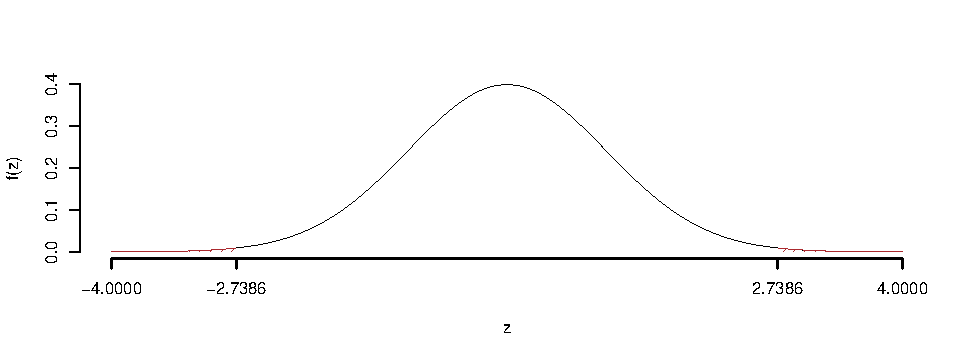
\includegraphics{Esami_passati_con_soluzioni_files/figure-latex/05-test-18,-1} \end{center}

\textbf{Rifiuto} \(H_0\) all'1\%,

\(0.001<p_\text{value}<0.01\), \emph{molto significativo} \(\fbox{**}\).

\end{sol}

\chapter{Test del Chi-quadro per indipendenza}\label{test-del-chi-quadro-per-indipendenza}

\section{Esercizio 1}\label{esercizio-1}

In uno studio sulle preferenze di gusti di gelato è stato chiesto ad un campione di 200 persone, divise tra 100 uomini e 100 donne, di esprimere la propria preferenza tra quattro gusti di gelato (Cioccolato, Fragola, Vaniglia e Limone).

Qui di seguito è riportata la tavola di contingenza:

\begin{table}[H]
\centering
\begin{tabular}{>{}lrrrrr}
\toprule
  & Cioccolato & Fragola & Vaniglia & Limone & Tot\\
\midrule
\textbf{Uomo} & 25 & 15 & 30 & 40 & 110\\
\textbf{Donna} & 20 & 10 & 40 & 30 & 100\\
\textbf{Tot} & 45 & 25 & 70 & 70 & 210\\
\bottomrule
\end{tabular}
\end{table}

Testare l'ipotesi che vi sia indipendenza tra genere e preferenza tra le profumazioni.

\begin{sol}
\textbf{Test \(\chi^2\) per indipendenza}

\(\fbox{A}\) FORMULAZIONE DELLE IPOTESI
\[
\Big\{H_0:\pi_{ij}=\pi_{i\bullet}\pi_{\bullet j}
\]
\(\fbox{B}\) SCELTA E CALCOLO STATISTICA-TEST, \(\chi^2\)

Si usa il test \(\chi^2\), si crea la tabella delle frequenze teoriche
\[
n_{ij}^*=\frac{n_{i\bullet}n_{\bullet j}}{n}
\]

\begin{table}[H]
\centering
\begin{tabular}{>{}lrrrr}
\toprule
  & Cioccolato & Fragola & Vaniglia & Limone\\
\midrule
\textbf{Uomo} & 23.57 & 13.1 & 36.67 & 36.67\\
\textbf{Donna} & 21.43 & 11.9 & 33.33 & 33.33\\
\bottomrule
\end{tabular}
\end{table}

La tabella delle distanze
\[
\frac{(n_{ij}-n_{ij}^*)^2}{n_{ij}^*}
\]

\begin{table}[H]
\centering
\begin{tabular}{>{}lrrrr}
\toprule
  & Cioccolato & Fragola & Vaniglia & Limone\\
\midrule
\textbf{Uomo} & 0.087 & 0.277 & 1.212 & 0.303\\
\textbf{Donna} & 0.095 & 0.305 & 1.333 & 0.333\\
\bottomrule
\end{tabular}
\end{table}

\[
    \chi^2_{obs}= 3.945 
  \]

i \(gdl\)

\[
    ( 2 -1)\times( 4 -1)= 3 
  \]

\(\fbox{C}\) CONCLUSIONE

I valori critici sono

\(\chi^2_{3;0.1}=6.2514\); \(\chi^2_{3;0.05}=7.8147\); \(\chi^2_{3;0.01}=11.3449\); \(\chi^2_{3;0.001}=16.2662\)

Siccome

\begin{center}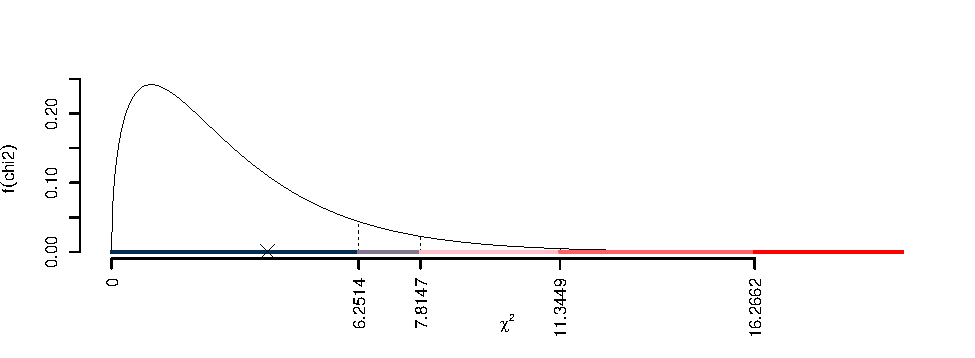
\includegraphics{Esami_passati_con_soluzioni_files/figure-latex/05a-chi2-2-1} \end{center}

Il \(p_{\text{value}}\) è

\[ p_{\text{value}} = P(\chi^2_{3}>3.95)=0.266914089227996 \]

Attenzione il calcolo del \(p_\text{value}\) con la distribuzione \(\chi^2\) è puramente illustrativo e non può essere riprodotto senza una calcolatrice statistica adeguata.\[
 0.1 \leq p_\text{value}= 0.2669 < 1 
\]

\end{sol}

\section{Esercizio 2}\label{esercizio-2}

In uno studio sulle preferenze di bevande è stato chiesto ad un campione di 180 persone di esprimere la propria preferenza tra tre tipi di bevande (Acqua, Succo d'arancia e Bibita gassata). Le persone sono state suddivise in due gruppi, chi mangia regolarmente frutta e chi no.

Qui di seguito è riportata la tavola di contingenza:

\begin{table}[H]
\centering
\begin{tabular}{>{}lrrrr}
\toprule
  & Acqua & Succo d'arancia & Bibita gassata & Tot\\
\midrule
\textbf{consuma frutta} & 40 & 30 & 20 & 90\\
\textbf{non consuma frutta} & 30 & 25 & 35 & 90\\
\textbf{Tot} & 70 & 55 & 55 & 180\\
\bottomrule
\end{tabular}
\end{table}

Testare l'ipotesi che vi sia indipendenza tra consumo abituale di frutta e preferenza di bevande.

\begin{sol}
\textbf{Test \(\chi^2\) per indipendenza}

\(\fbox{A}\) FORMULAZIONE DELLE IPOTESI
\[
\Big\{H_0:\pi_{ij}=\pi_{i\bullet}\pi_{\bullet j}
\]
\(\fbox{B}\) SCELTA E CALCOLO STATISTICA-TEST, \(\chi^2\)

Si usa il test \(\chi^2\), si crea la tabella delle frequenze teoriche
\[
n_{ij}^*=\frac{n_{i\bullet}n_{\bullet j}}{n}
\]

\begin{table}[H]
\centering
\begin{tabular}{>{}lrrr}
\toprule
  & Acqua & Succo d'arancia & Bibita gassata\\
\midrule
\textbf{consuma frutta} & 35 & 27.5 & 27.5\\
\textbf{non consuma frutta} & 35 & 27.5 & 27.5\\
\bottomrule
\end{tabular}
\end{table}

La tabella delle distanze
\[
\frac{(n_{ij}-n_{ij}^*)^2}{n_{ij}^*}
\]

\begin{table}[H]
\centering
\begin{tabular}{>{}lrrr}
\toprule
  & Acqua & Succo d'arancia & Bibita gassata\\
\midrule
\textbf{consuma frutta} & 0.714 & 0.227 & 2.045\\
\textbf{non consuma frutta} & 0.714 & 0.227 & 2.045\\
\bottomrule
\end{tabular}
\end{table}

\[
    \chi^2_{obs}= 5.974 
  \]

i \(gdl\)

\[
    ( 2 -1)\times( 3 -1)= 2 
  \]

\(\fbox{C}\) CONCLUSIONE

I valori critici sono

\(\chi^2_{2;0.1}=4.6052\); \(\chi^2_{2;0.05}=5.9915\); \(\chi^2_{2;0.01}=9.2103\); \(\chi^2_{2;0.001}=13.8155\)

Siccome \(4.6052<\chi^2_\text{obs}=5.974<5.9915\), indecisione sul rifiuto di \(H_0\) al 10\%, \(0.05<p_\text{value}<0.1\),

\emph{marginalmente significativo} \(\fbox{.}\).

\begin{center}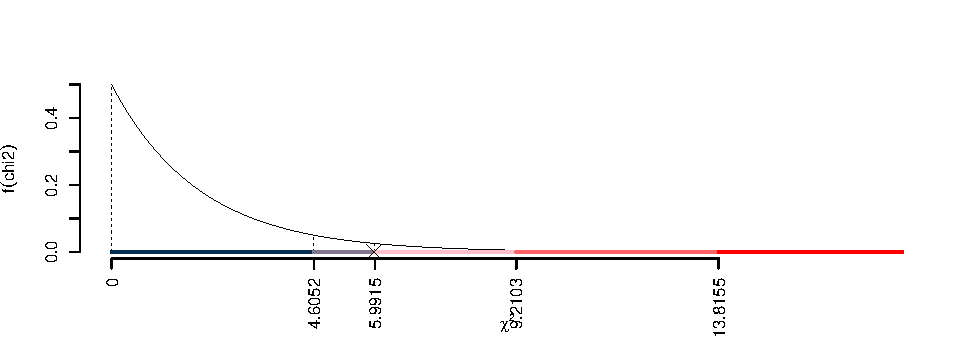
\includegraphics{Esami_passati_con_soluzioni_files/figure-latex/05a-chi2-4-1} \end{center}

Il \(p_{\text{value}}\) è

\[ p_{\text{value}} = P(\chi^2_{2}>5.97)=0.0505395035491347 \]

Attenzione il calcolo del \(p_\text{value}\) con la distribuzione \(\chi^2\) è puramente illustrativo e non può essere riprodotto senza una calcolatrice statistica adeguata.\[
 0.05 \leq p_\text{value}= 0.05054 < 0.1 
\]

\end{sol}

\section{Esercizio 3}\label{esercizio-3}

In uno studio sulle opinioni riguardo al tema del ``Matrimonio tra persone dello stesso sesso'' è stato chiesto ad un campione di 180 persone di esprimere la propria opinione scegliendo tra tre possibilità (Sostenitore, Neutrale, Contrario). Le persone sono state suddivise in due gruppi, ``Elettori di Destra'' e ``Elettori di Sinistra''.

Qui di seguito è riportata la tavola di contingenza:

\begin{table}[H]
\centering
\begin{tabular}{>{}lrrrr}
\toprule
  & Sostenitore & Neutrale & Contrario & Tot\\
\midrule
\textbf{Elettori di Destra} & 40 & 10 & 35 & 85\\
\textbf{Elettori di Sinistra} & 30 & 25 & 20 & 75\\
\textbf{Tot} & 70 & 35 & 55 & 160\\
\bottomrule
\end{tabular}
\end{table}

Testare l'ipotesi che vi sia indipendenza tra l'opinione riguardo al tema ``Matrimonio tra persone dello stesso sesso'' e l'appartenenza ai gruppi ``Elettori di Destra'' e ``Elettori di Sinistra''.

\begin{sol}
\textbf{Test \(\chi^2\) per indipendenza}

\(\fbox{A}\) FORMULAZIONE DELLE IPOTESI
\[
\Big\{H_0:\pi_{ij}=\pi_{i\bullet}\pi_{\bullet j}
\]
\(\fbox{B}\) SCELTA E CALCOLO STATISTICA-TEST, \(\chi^2\)

Si usa il test \(\chi^2\), si crea la tabella delle frequenze teoriche
\[
n_{ij}^*=\frac{n_{i\bullet}n_{\bullet j}}{n}
\]

\begin{table}[H]
\centering
\begin{tabular}{>{}lrrr}
\toprule
  & Sostenitore & Neutrale & Contrario\\
\midrule
\textbf{Elettori di Destra} & 37.19 & 18.59 & 29.22\\
\textbf{Elettori di Sinistra} & 32.81 & 16.41 & 25.78\\
\bottomrule
\end{tabular}
\end{table}

La tabella delle distanze
\[
\frac{(n_{ij}-n_{ij}^*)^2}{n_{ij}^*}
\]

\begin{table}[H]
\centering
\begin{tabular}{>{}lrrr}
\toprule
  & Sostenitore & Neutrale & Contrario\\
\midrule
\textbf{Elettori di Destra} & 0.213 & 3.972 & 1.144\\
\textbf{Elettori di Sinistra} & 0.241 & 4.501 & 1.296\\
\bottomrule
\end{tabular}
\end{table}

\[
    \chi^2_{obs}= 11.37 
  \]

i \(gdl\)

\[
    ( 2 -1)\times( 3 -1)= 2 
  \]

\(\fbox{C}\) CONCLUSIONE

I valori critici sono

\(\chi^2_{2;0.1}=4.6052\); \(\chi^2_{2;0.05}=5.9915\); \(\chi^2_{2;0.01}=9.2103\); \(\chi^2_{2;0.001}=13.8155\)

Siccome \(9.2103<\chi^2_\text{obs}=11.3675<13.8155\), quindi \textbf{rifiuto} \(H_0\) all'1\%, \(0.001<p_\text{value}<0.01\),

\emph{molto significativo} \(\fbox{**}\).

\begin{center}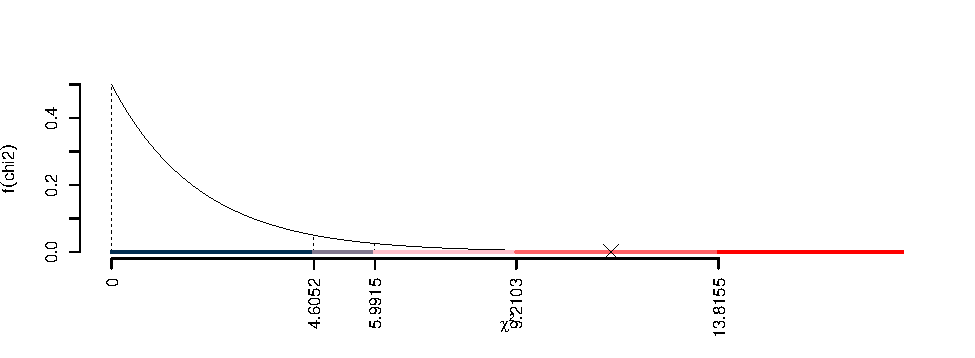
\includegraphics{Esami_passati_con_soluzioni_files/figure-latex/05a-chi2-6-1} \end{center}

Il \(p_{\text{value}}\) è

\[ p_{\text{value}} = P(\chi^2_{2}>11.37)=0.00339653324963196 \]

Attenzione il calcolo del \(p_\text{value}\) con la distribuzione \(\chi^2\) è puramente illustrativo e non può essere riprodotto senza una calcolatrice statistica adeguata.\[
 0.001 \leq p_\text{value}= 0.003397 < 0.01 
\]

\end{sol}

\section{Esercizio 4}\label{esercizio-4}

In uno studio sociologico sulle preferenze di attività ricreative è stato chiesto ad un campione di 270 persone di esprimere la propria preferenza tra tre tipi di attività (Sport, Lettura e Arte). Le persone sono state suddivise in tre gruppi, ``Giovani'', ``Adulti'' e ``Anziani''.

Qui di seguito è riportata la tavola di contingenza:

\begin{table}[H]
\centering
\begin{tabular}{>{}lrrrr}
\toprule
  & Sport & Lettura & Arte & Tot\\
\midrule
\textbf{Giovani} & 50 & 40 & 20 & 110\\
\textbf{Adulti} & 30 & 60 & 25 & 115\\
\textbf{Anziani} & 20 & 10 & 40 & 70\\
\textbf{Tot} & 100 & 110 & 85 & 295\\
\bottomrule
\end{tabular}
\end{table}

Testare l'ipotesi che vi sia indipendenza tra la preferenza per le attività ricreative e l'età.

\begin{sol}
\textbf{Test \(\chi^2\) per indipendenza}

\(\fbox{A}\) FORMULAZIONE DELLE IPOTESI
\[
\Big\{H_0:\pi_{ij}=\pi_{i\bullet}\pi_{\bullet j}
\]
\(\fbox{B}\) SCELTA E CALCOLO STATISTICA-TEST, \(\chi^2\)

Si usa il test \(\chi^2\), si crea la tabella delle frequenze teoriche
\[
n_{ij}^*=\frac{n_{i\bullet}n_{\bullet j}}{n}
\]

\begin{table}[H]
\centering
\begin{tabular}{>{}lrrr}
\toprule
  & Sport & Lettura & Arte\\
\midrule
\textbf{Giovani} & 37.29 & 41.02 & 31.70\\
\textbf{Adulti} & 38.98 & 42.88 & 33.14\\
\textbf{Anziani} & 23.73 & 26.10 & 20.17\\
\bottomrule
\end{tabular}
\end{table}

La tabella delle distanze
\[
\frac{(n_{ij}-n_{ij}^*)^2}{n_{ij}^*}
\]

\begin{table}[H]
\centering
\begin{tabular}{>{}lrrr}
\toprule
  & Sport & Lettura & Arte\\
\midrule
\textbf{Giovani} & 4.334 & 0.025 & 4.315\\
\textbf{Adulti} & 2.070 & 6.834 & 1.997\\
\textbf{Anziani} & 0.586 & 9.933 & 19.497\\
\bottomrule
\end{tabular}
\end{table}

\[
    \chi^2_{obs}= 49.59 
  \]

i \(gdl\)

\[
    ( 3 -1)\times( 3 -1)= 4 
  \]

\(\fbox{C}\) CONCLUSIONE

I valori critici sono

\(\chi^2_{4;0.1}=7.7794\); \(\chi^2_{4;0.05}=9.4877\); \(\chi^2_{4;0.01}=13.2767\); \(\chi^2_{4;0.001}=18.4668\)

Siccome \(\chi^2_\text{obs}=49.5915>18.4668\), quindi \textbf{rifiuto} \(H_0\) sotto all'1‰, \(p_\text{value}<0.001\),

\emph{estremamente significativo} \(\fbox{***}\).

\begin{center}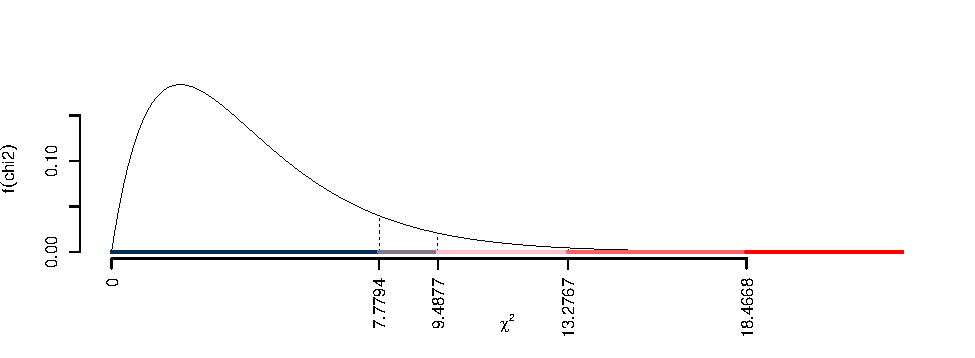
\includegraphics{Esami_passati_con_soluzioni_files/figure-latex/05a-chi2-8-1} \end{center}

Il \(p_{\text{value}}\) è

\[ p_{\text{value}} = P(\chi^2_{4}>49.59)=0.000000000439748015779173 \]

Attenzione il calcolo del \(p_\text{value}\) con la distribuzione \(\chi^2\) è puramente illustrativo e non può essere riprodotto senza una calcolatrice statistica adeguata.\[
 0 \leq p_\text{value}= 0.0000000004397 < 0.001 
\]

\end{sol}

\chapter{Test del Chi-quadro per conformità}\label{test-del-chi-quadro-per-conformituxe0}

\section{Esercizio 1}\label{esercizio-1-1}

L'Associazione Bar dell'Emilia Romagna ha condotto un'indagine sulle preferenze delle bevande dei clienti dei bar della regione. Durante una settimana, sono stati intervistati 250 clienti di vari bar della zona. L'associazione è interessata a capire se le preferenze dei clienti per le bevande differiscono dalla media nazionale.

Qui di seguito è riportata la tabella delle preferenze dei clienti dei bar dell'Emilia Romagna:

\begin{table}[H]
\centering
\begin{tabular}{lllll}
\toprule
  & Caffè & Tè & Altro & Totale\\
\midrule
Dati Associazione & $100$ & $88$ & $62$ & $250$\\
Media Nazionale & $50\%$ & $30\%$ & $20\%$ & $100\%$\\
\bottomrule
\end{tabular}
\end{table}

Testare l'ipotesi che le preferenze dei clienti dei bar dell'Emilia Romagna per le bevande differiscano dalla media nazionale.

\begin{sol}
\textbf{Test \(\chi^2\) per conformità}

\(\fbox{A}\) Formulazione delle ipotesi
\[
\{H_0:\pi_\text{ Dati Associazione }= \pi_\text{ Media Nazionale },~~\forall j
\]
\(\fbox{B}\) Scelta e calcolo della statistica test.

Si tratta di un test chi quadro di conformità.
\[
n^*_j = n\cdot \pi^*_{\text{ Media Nazionale },j} 
\]

La tabella delle distanze:

\begin{table}[H]
\centering
\begin{tabular}{lrrrr}
\toprule
  & Caffè & Tè & Altro & Tot\\
\midrule
Dati Associazione & 100.0 & 88.000 & 62.00 & 250.00\\
Media Nazionale & 0.5 & 0.300 & 0.20 & 1.00\\
$n_j^*$ & 125.0 & 75.000 & 50.00 & 250.00\\
$\chi^2$ & 5.0 & 2.253 & 2.88 & 10.13\\
\bottomrule
\end{tabular}
\end{table}

\[
    \chi^2_{obs}= 10.13 
  \]

i \(gdl\)

\[
    ( 3 -1)= 2 
  \]

\(\fbox{C}\) CONCLUSIONE

I valori critici sono

\(\chi^2_{2;0.1}=4.61\); \(\chi^2_{2;0.05}=5.99\); \(\chi^2_{2;0.01}=9.21\); \(\chi^2_{2;0.001}=13.82\)

Siccome \(9.21<\chi^2_\text{obs}=10.1333<13.82\), quindi \textbf{rifiuto} \(H_0\) all'1\%, \(0.001<p_\text{value}<0.01\),

\emph{molto significativo} \(\fbox{**}\).

\begin{center}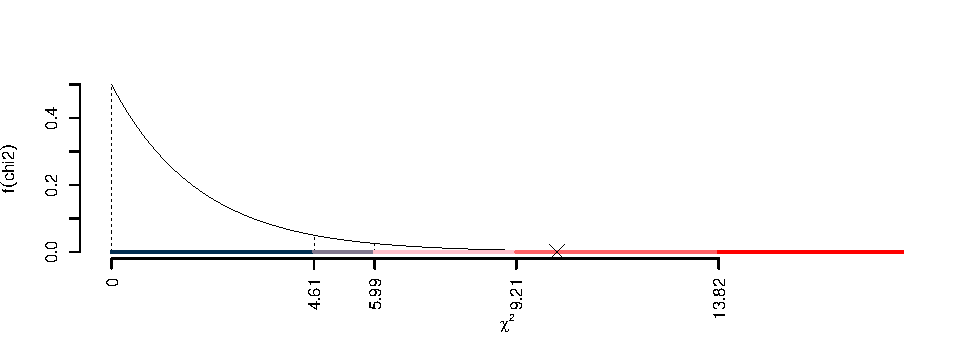
\includegraphics{Esami_passati_con_soluzioni_files/figure-latex/05a-chi2-10-1} \end{center}

Il \(p_{\text{value}}\) è

\[ p_{\text{value}} = P(\chi^2_{2}>10.13)=0.00631391090280442 \]

Attenzione il calcolo del \(p_\text{value}\) con la distribuzione \(\chi^2\) è puramente illustrativo e non può essere riprodotto senza una calcolatrice statistica adeguata.\[
 0.001 \leq p_\text{value}= 0.006314 < 0.01 
\]

\end{sol}

\section{Esercizio 2}\label{esercizio-2-1}

L'Associazione dei Ristoranti dell'Emilia Romagna ha condotto un'indagine sulle preferenze culinarie dei clienti dei ristoranti della regione. Durante una settimana, sono stati intervistati 300 clienti di vari ristoranti. L'associazione è interessata a capire se le preferenze dei clienti per le tipologie di cucina offerte differiscono dalla media nazionale.

Qui di seguito è riportata la tabella delle preferenze dei clienti dei ristoranti dell'Emilia Romagna e le percentuali nazionali:

\begin{table}[H]
\centering
\begin{tabular}{lllllll}
\toprule
  & Italiana & Giapponese & Messicana & Mediterranea & Vegetariana & Totale\\
\midrule
Dati Associazione & $147$ & $74$ & $15$ & $59$ & $6$ & $301$\\
Media Nazionale & $40\%$ & $15\%$ & $5\%$ & $35\%$ & $5\%$ & $100\%$\\
\bottomrule
\end{tabular}
\end{table}

Testare l'ipotesi che le preferenze dei clienti dei bar dell'Emilia Romagna per le bevande differiscano dalla media nazionale.

\begin{sol}
\textbf{Test \(\chi^2\) per conformità}

\(\fbox{A}\) Formulazione delle ipotesi
\[
\{H_0:\pi_\text{ Dati Associazione }= \pi_\text{ Media Nazionale },~~\forall j
\]
\(\fbox{B}\) Scelta e calcolo della statistica test.

Si tratta di un test chi quadro di conformità.
\[
n^*_j = n\cdot \pi^*_{\text{ Media Nazionale },j} 
\]

La tabella delle distanze:

\begin{table}[H]
\centering
\begin{tabular}{lrrrrrr}
\toprule
  & Italiana & Giapponese & Messicana & Mediterranea & Vegetariana & Tot\\
\midrule
Dati Associazione & 147.000 & 74.00 & 15.0000 & 59.00 & 6.000 & 301.00\\
Media Nazionale & 0.400 & 0.15 & 0.0500 & 0.35 & 0.050 & 1.00\\
$n_j^*$ & 120.400 & 45.15 & 15.0500 & 105.35 & 15.050 & 301.00\\
$\chi^2$ & 5.877 & 18.43 & 0.0002 & 20.39 & 5.442 & 50.15\\
\bottomrule
\end{tabular}
\end{table}

\[
    \chi^2_{obs}= 50.15 
  \]

i \(gdl\)

\[
    ( 5 -1)= 4 
  \]

\(\fbox{C}\) CONCLUSIONE

I valori critici sono

\(\chi^2_{4;0.1}=7.7794\); \(\chi^2_{4;0.05}=9.4877\); \(\chi^2_{4;0.01}=13.2767\); \(\chi^2_{4;0.001}=18.4668\)

Siccome \(\chi^2_\text{obs}=50.1457>18.4668\), quindi \textbf{rifiuto} \(H_0\) sotto all'1‰, \(p_\text{value}<0.001\),

\emph{estremamente significativo} \(\fbox{***}\).

\begin{center}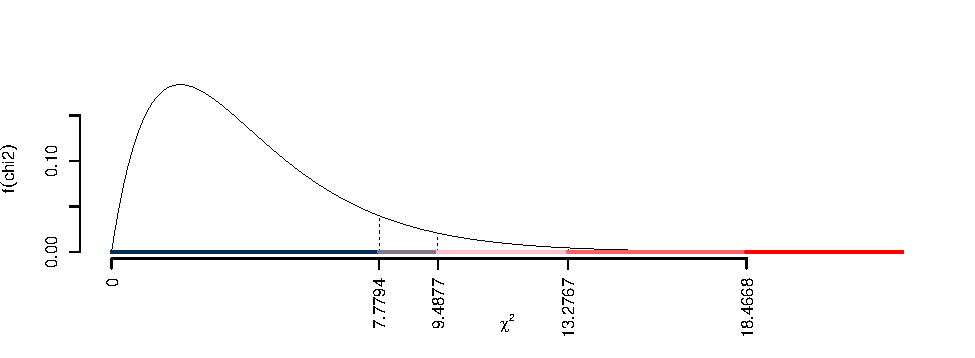
\includegraphics{Esami_passati_con_soluzioni_files/figure-latex/05a-chi2-12-1} \end{center}

Il \(p_{\text{value}}\) è

\[ p_{\text{value}} = P(\chi^2_{4}>50.15)=0.000000000335962035968862 \]

Attenzione il calcolo del \(p_\text{value}\) con la distribuzione \(\chi^2\) è puramente illustrativo e non può essere riprodotto senza una calcolatrice statistica adeguata.\[
 0 \leq p_\text{value}= 0.000000000336 < 0.001 
\]

\end{sol}

\chapter{Esericizi sulla Regressione}\label{esericizi-sulla-regressione}

\section{Esercizio (Dati maternità USA)}\label{esercizio-dati-maternituxe0-usa}

\subsection{I dati}\label{i-dati}

Il dataset di dimensioni \(n = 51\) è relativo ai 50 stati e al Distretto di Columbia negli Stati Uniti. Le variabili sono

\begin{itemize}
\tightlist
\item
  \(y =\) \emph{il tasso di natalità dell'anno 2002 per 1000 femmine di età compresa tra 15 e 17 anni}\\
\item
  \(x =\) \emph{il tasso di povertà, che rappresenta la percentuale della popolazione dello stato che vive in famiglie con redditi al di sotto della soglia di povertà definita dal governo federale.}
\end{itemize}

(Fonte dei dati: Mind On Statistics, 3a edizione, Utts and Heckard).

\subsection{La matrice dei dati}\label{la-matrice-dei-dati}

\begin{table}[H]
\centering
\begin{tabular}{rlrr}
\toprule
$i$ & Stato & Tasso di povertà & Tasso di natalità 15-17\\
\midrule
1 & Alabama & 20.1 & 31.5\\
2 & Alaska & 7.1 & 18.9\\
3 & Arizona & 16.1 & 35.0\\
4 & Arkansas & 14.9 & 31.6\\
5 & California & 16.7 & 22.6\\
6 & Colorado & 8.8 & 26.2\\
7 & Connecticut & 9.7 & 14.1\\
8 & Delaware & 10.3 & 24.7\\
9 & District of Columbia & 22.0 & 44.8\\
10 & Florida & 16.2 & 23.2\\
11 & Georgia & 12.1 & 31.4\\
12 & Hawaii & 10.3 & 17.7\\
13 & Idaho & 14.5 & 18.4\\
14 & Illinois & 12.4 & 23.4\\
15 & Indiana & 9.6 & 22.6\\
16 & Iowa & 12.2 & 16.4\\
17 & Kansas & 10.8 & 21.4\\
18 & Kentucky & 14.7 & 26.5\\
19 & Louisiana & 19.7 & 31.7\\
20 & Maine & 11.2 & 11.9\\
21 & Maryland & 10.1 & 20.0\\
22 & Massachusetts & 11.0 & 12.5\\
23 & Michigan & 12.2 & 18.0\\
24 & Minnesota & 9.2 & 14.2\\
25 & Mississippi & 23.5 & 37.6\\
26 & Missouri & 9.4 & 22.2\\
27 & Montana & 15.3 & 17.8\\
28 & Nebraska & 9.6 & 18.3\\
29 & Nevada & 11.1 & 28.0\\
30 & New Hampshire & 5.3 & 8.1\\
31 & New Jersey & 7.8 & 14.7\\
32 & New Mexico & 25.3 & 37.8\\
33 & New York & 16.5 & 15.7\\
34 & North Carolina & 12.6 & 28.6\\
35 & North Dakota & 12.0 & 11.7\\
36 & Ohio & 11.5 & 20.1\\
37 & Oklahoma & 17.1 & 30.1\\
38 & Oregon & 11.2 & 18.2\\
39 & Pennsylvania & 12.2 & 17.2\\
40 & Rhode Island & 10.6 & 19.6\\
41 & South Carolina & 19.9 & 29.2\\
42 & South Dakota & 14.5 & 17.3\\
43 & Tennessee & 15.5 & 28.2\\
44 & Texas & 17.4 & 38.2\\
45 & Utah & 8.4 & 17.8\\
46 & Vermont & 10.3 & 10.4\\
47 & Virginia & 10.2 & 19.0\\
48 & Washington & 12.5 & 16.8\\
49 & West Virginia & 16.7 & 21.5\\
50 & Wisconsin & 8.5 & 15.9\\
51 & Wyoming & 12.2 & 17.7\\
\bottomrule
\end{tabular}
\end{table}

\subsection{La rappresentazione dei dati}\label{la-rappresentazione-dei-dati}

\begin{center}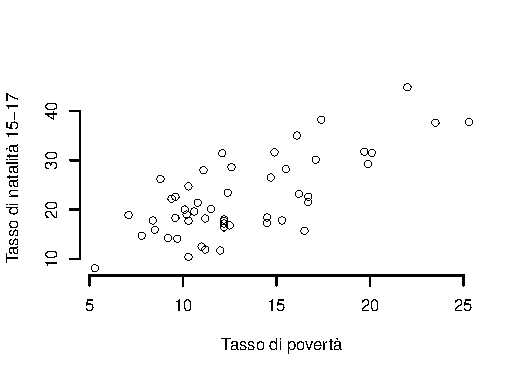
\includegraphics{Esami_passati_con_soluzioni_files/figure-latex/06-regr-45-1} \end{center}

Tutta l'informazione sul modello di regressione lineare semplice è contenuta nelle
seguenti statistiche
\[
\sum_{i=1}^n x_i=        669.00,
~~\sum_{i=1}^n y_i=      1~136.40,\\
~~\sum_{i=1}^n x_i^2=    9~690.44,
~~\sum_{i=1}^ny_i^2=     28~556.56,\\
\sum_{i=1}^n x_i y_i= 16~163.14
\]

da cui ricaviamo tutte le altre statistiche di interesse

\begin{alignat*}{3}
 \bar x & =  \frac 1 n \sum_{i=1}^n x_i  = 13.1176 &
\hat\sigma_X^2 & =  \frac 1 n \sum_{i=1}^n x_i^2 - \bar x^2  = 17.936 &\\
 \bar y & =  \frac 1 n \sum_{i=1}^n y_i   = 22.2824 &
\hat\sigma_Y^2 & =  \frac 1 n \sum_{i=1}^n y_i^2 - \bar y^2  = 63.4293 &\\
 \text{cov}(x,y) & = \frac 1 n \sum_{i=1}^n x_iy_i -\bar x\bar y  = 24.6323 & 
r & = \frac{\text{cov}(x,y)}{\hat\sigma_X \hat\sigma_Y }  = 0.7303 &\\
\hat\beta_1 & = \frac{\text{cov}(x,y)}{\hat\sigma_X^2} = 1.3733 & 
\hat\beta_0 & = \bar y  - \hat\beta_1\bar x = 4.2673. &\\
\hat\sigma_\varepsilon^2 & = \hat\sigma_Y^2(1-r^2)=29.6007 &
S_\varepsilon^2 & = \frac{n}{n-2}\hat\sigma_\varepsilon^2 = 30.8089\\
\hat\sigma_\varepsilon & = \hat\sigma_Y\sqrt{(1-r^2)}=5.4407 & \qquad
S_\varepsilon & = \sqrt{\frac{n}{n-2}}\hat\sigma_\varepsilon = 5.5506\\
\end{alignat*}

\begin{center}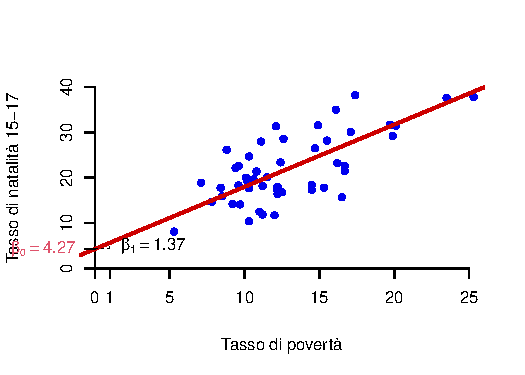
\includegraphics{Esami_passati_con_soluzioni_files/figure-latex/06-regr-46-1} \end{center}

\begin{center}\rule{0.5\linewidth}{0.5pt}\end{center}

Valutare la bontà di adattamento del modello precedente.

\begin{sol}
\begin{eqnarray*}
r&=&\frac{\text{cov}(X,Y)}{\sigma_X\sigma_Y}=\frac{ 24.63 }{ 4.235 \times 7.964 }= 0.7303 \\ 
r^2&=& 0.5333 < 0.75
\end{eqnarray*}

Il modello \textbf{non} si adatta bene ai dati.

Il modello spiega il \(53.33\%\) della variabilità totale della \(Y\).

\end{sol}

\begin{center}\rule{0.5\linewidth}{0.5pt}\end{center}

Fornire una interpretazione dei parametri della retta di regressione.

\begin{sol}
I parametri della retta di regressione sono \(\beta_{0}\) e \(\beta_{1}\).
Il primo, \(\beta_{0},\) rappresenta l'intercetta della retta,
ovvero il punto in cui la retta interseca l'asse delle ordinate.
Il secondo parametro, \(\beta_{1}\), rappresenta la pendenza della
retta (chiamato anche coefficiente angolare), ovvero l'incremento
verticale corrispondente a un incremento orizzontale unitario e
coincide, perciò, con la tangente dell'angolo compreso fra la
retta e l'asse delle ascisse.

In questo caso, il tasso di natalità per le under 15,
secondo il modello stimato, è dato da
\[Y= 4.2673 + 1.3733 X\]

ossia, è composto da un quantitativo fisso di \(4.2673\) di tasso di natalità per le under 15 in un ipotetico stato a con tasso di povertà zero (\(x=0\)), a cui si aggiunge un incremento di \(1.3733\) per ogni incremento unitario del tasso di povertà.

\end{sol}

\begin{center}\rule{0.5\linewidth}{0.5pt}\end{center}

Determinare il residuo per lo stato del Colorado \(i=6\)
uguale 6, ossia per \(x=6\).

\begin{sol}
\begin{eqnarray*}
\hat y_i &=&\hat\beta_0+\hat\beta_1 x_i=\\ 
&=& 4.267 + 1.3733 \times 8.8 = 16.35 \\ 
\hat \varepsilon_i &=& y_i-\hat y_i\\ 
&=& 26.2 - 16.3527 = 9.847  
\end{eqnarray*}

\end{sol}

\begin{center}\rule{0.5\linewidth}{0.5pt}\end{center}

Verificare l'ipotesi che l'intercetta della retta di regressione sia uguale a
zero contro l'alternativa che sia diversa da zero.

\begin{sol}
\begin{eqnarray*}
\hat{\sigma_\varepsilon}^2&=&(1-r^2)\hat\sigma_Y^2\\
&=& (1- 0.5333 )\times 63.43 \\
   &=&  29.6 \\
   S_\varepsilon^2 &=& \frac{n} {n-2} \hat{\sigma_\varepsilon}^2\\
   &=&  \frac{ 51 } { 51 -2} \hat{\sigma_\varepsilon}^2 \\
 &=&  \frac{ 51 } { 51 -2} \times  29.6  =  30.81  
\end{eqnarray*}

E quindi\begin{eqnarray*}
V(\hat\beta_{0}) &=& \sigma_{\varepsilon}^{2} \left( \frac{1} {n}  +  \frac{\bar{x}^{2}} {n \hat{\sigma}^{2}_{X}} \right)\\
\widehat{V(\hat\beta_{0})} &=& S_{\varepsilon}^{2}\left( \frac{1} {n}  +  \frac{\bar{x}^{2}} {n \hat{\sigma}^{2}_{X}} \right)\ \\
 &=&  30.81 \times\left( \frac{1} { 51 }  +  \frac{ 13.12 ^{2}} { 51 \times  17.94 } \right)\\
 \widehat{SE(\hat\beta_{0})}        &=&  \sqrt{ 6.4 }\\
 &=&  2.53 
\end{eqnarray*}
\(\fbox{A}\) FORMULAZIONE DELLE IPOTESI

\[\begin{cases}
   H_0: \beta_0 = \beta_{0;H_0}=0 \\
   H_1: \beta_0 \neq \beta_{0;H_0}=0 
   \end{cases}\]

\(\fbox{B}\) SCELTA E CALCOLO STATISTICA-TEST, \(T\)
Test su un coefficiente di regressione: \(\Rightarrow\) t-Test.

\begin{eqnarray*}
 \frac{\hat\beta_{ 0 } - \beta_{ 0 ;H_0}} {\widehat{SE(\hat\beta_{ 0 })}}&\sim&t_{n-2}\\
   t_{\text{obs}}
&=& \frac{ ( 4.267 -  0 )} { 2.53 }
 =   1.687 \, .
\end{eqnarray*}

\(\fbox{C}\) CONCLUSIONE

Siccome \(H_1\) è bilaterale, considereremo \(\alpha/2\),
anziché \(\alpha\)

\(\alpha=0.1, 0.05, 0.01, 0.001\) e quindi \(\alpha/2=0.05, 0.025, 0.005, 0.0005\)

I valori critici sono

\(t_{51-2;0.05}=1.6766\); \(t_{51-2;0.025}=2.0096\); \(t_{51-2;0.005}=2.68\); \(t_{51-2;0.0005}=3.5004\)

Siccome \(1.6766<|t_\text{obs}|=1.6868<2.0096\), indecisione sul rifiuto di \(H_0\) al 10\%,

\(0.05<p_\text{value}<0.1\), \emph{marginalmente significativo} \(\fbox{.}\).

\begin{center}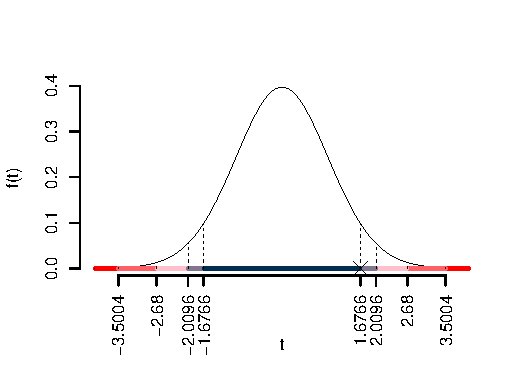
\includegraphics{Esami_passati_con_soluzioni_files/figure-latex/06-regr-3,-1} \end{center}

Il \(p_{\text{value}}\) è

\[ p_{\text{value}} = P(|T_{51-2}|>|1.69|)=2P(T_{51-2}>1.69)=0.097990 \]

Attenzione il calcolo del \(p_\text{value}\) con la \(T\) è puramente illustrativo e non può essere riprodotto senza una calcolatrice statistica adeguata.\[
 0.05 < p_\text{value}= 0.097990 \leq 0.1 
\]

\end{sol}

\begin{center}\rule{0.5\linewidth}{0.5pt}\end{center}

Verificare l'ipotesi che la pendenza della retta di regressione sia uguale a 0
contro l'alternativa che sia diversa da 0.

\begin{sol}
\begin{eqnarray*}
\hat{\sigma_\varepsilon}^2&=&(1-r^2)\hat\sigma_Y^2\\
&=& (1- 0.5333 )\times 63.43 \\
   &=&  29.6 \\
   S_\varepsilon^2 &=& \frac{n} {n-2} \hat{\sigma_\varepsilon}^2\\
   &=&  \frac{ 51 } { 51 -2} \hat{\sigma_\varepsilon}^2 \\
 &=&  \frac{ 51 } { 51 -2} \times  29.6  =  30.81  
\end{eqnarray*}

E quindi\begin{eqnarray*}
V(\hat\beta_{1}) &=& \frac{\sigma_{\varepsilon}^{2}} {n \hat{\sigma}^{2}_{X}} \\
\widehat{V(\hat\beta_{1})} &=& \frac{S_{\varepsilon}^{2}} {n \hat{\sigma}^{2}_{X}} \\
 &=& \frac{ 30.81 } { 51 \times  17.94 } =  0.0337 \\
 \widehat{SE(\hat\beta_{1})}        &=&  \sqrt{ 0.0337 }\\
 &=&  0.1836 
\end{eqnarray*}

\(\fbox{A}\) FORMULAZIONE DELLE IPOTESI

\[\begin{cases}
   H_0: \beta_1 = \beta_{1;H_0}=0 \\
   H_1: \beta_1 > \beta_{1;H_0}=0 
   \end{cases}\]

\(\fbox{B}\) SCELTA E CALCOLO STATISTICA-TEST, \(T\)
Test su un coefficiente di regressione: \(\Rightarrow\) t-Test.

\begin{eqnarray*}
 \frac{\hat\beta_{ 1 } - \beta_{ 1 ;H_0}} {\widehat{SE(\hat\beta_{ 1 })}}&\sim&t_{n-2}\\
   t_{\text{obs}}
&=& \frac{ ( 1.373 -  0 )} { 0.1836 }
 =   7.481 \, .
\end{eqnarray*}

\(\fbox{C}\) CONCLUSIONE

Consideriamo \(\alpha=0.1, 0.05, 0.01, 0.001\)

I valori critici sono

\(t_{51-2;0.1}=1.2991\); \(t_{51-2;0.05}=1.6766\); \(t_{51-2;0.01}=2.4049\); \(t_{51-2;0.001}=3.2651\)

Siccome \(t_\text{obs}=7.4808>3.2651\), quindi \textbf{rifiuto} \(H_0\) sotto all'1‰,

\(p_\text{value}<0.001\), \emph{estremamente significativo} \(\fbox{***}\).

\begin{center}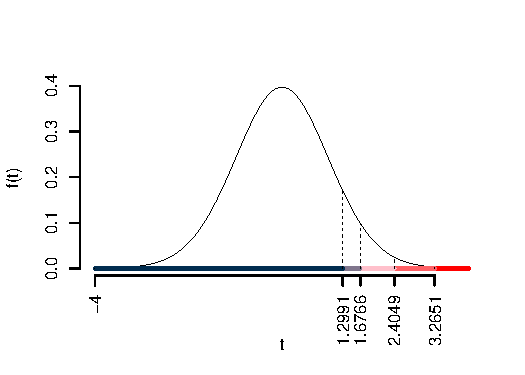
\includegraphics{Esami_passati_con_soluzioni_files/figure-latex/06-regr-4,-1} \end{center}

Il \(p_{\text{value}}\) è

\[ p_{\text{value}} = P(T_{51-2}>7.48)=6e-10 \]

Attenzione il calcolo del \(p_\text{value}\) con la \(T\) è puramente illustrativo e non può essere riprodotto senza una calcolatrice statistica adeguata.\[
 0 < p_\text{value}= 6e-10 \leq 0.001 
\]

\end{sol}

\begin{center}\rule{0.5\linewidth}{0.5pt}\end{center}

Un software professionale restituisce un output del genere

\begin{Shaded}
\begin{Highlighting}[]
\FunctionTok{head}\NormalTok{(data\_poverty,}\AttributeTok{n =} \DecValTok{10}\NormalTok{)}
\end{Highlighting}
\end{Shaded}

\begin{verbatim}
##                    state poverty_rate birth_rate
## 1               Alabama          20.1       31.5
## 2                Alaska           7.1       18.9
## 3               Arizona          16.1       35.0
## 4              Arkansas          14.9       31.6
## 5            California          16.7       22.6
## 6              Colorado           8.8       26.2
## 7           Connecticut           9.7       14.1
## 8              Delaware          10.3       24.7
## 9  District of Columbia          22.0       44.8
## 10              Florida          16.2       23.2
\end{verbatim}

\begin{Shaded}
\begin{Highlighting}[]
\NormalTok{modello }\OtherTok{\textless{}{-}} \FunctionTok{lm}\NormalTok{(}\AttributeTok{formula =}\NormalTok{ birth\_rate }\SpecialCharTok{\textasciitilde{}}\NormalTok{ poverty\_rate,}\AttributeTok{data =}\NormalTok{ data\_poverty)}
\FunctionTok{summary}\NormalTok{(modello)}
\end{Highlighting}
\end{Shaded}

\begin{verbatim}
## 
## Call:
## lm(formula = birth_rate ~ poverty_rate, data = data_poverty)
## 
## Residuals:
##     Min      1Q  Median      3Q     Max 
## -11.227  -3.655  -0.041   2.497  10.515 
## 
## Coefficients:
##              Estimate Std. Error t value     Pr(>|t|)    
## (Intercept)     4.267      2.530    1.69        0.098 .  
## poverty_rate    1.373      0.184    7.48 0.0000000012 ***
## ---
## Signif. codes:  0 '***' 0.001 '**' 0.01 '*' 0.05 '.' 0.1 ' ' 1
## 
## Residual standard error: 5.55 on 49 degrees of freedom
## Multiple R-squared:  0.533,  Adjusted R-squared:  0.524 
## F-statistic:   56 on 1 and 49 DF,  p-value: 0.00000000119
\end{verbatim}

\section{Esercizio 1}\label{esercizio-1-2}

Si sono raccolti i seguenti valori per la variabile indipendente
\(X\), indice delle importazioni, e la variabile dipendente \(Y\),
indice della produzione industriale (dati artificiali).

\small
\begin{table}[H]
\centering
\begin{tabular}{lrrrrrrrrrrrrrrrr}
\toprule
$i$ & 1 & 2 & 3 & 4 & 5 & 6 & 7 & 8 & 9 & 10 & 11 & 12 & 13 & 14 & 15 & 16\\
$x$ & 102 & 105 & 107 & 108 & 109 & 109 & 110 & 112 & 113 & 115 & 116 & 118 & 119 & 120 & 121 & 122\\
$y$ & 107 & 108 & 109 & 110 & 111 & 112 & 112 & 116 & 118 & 121 & 123 & 126 & 128 & 130 & 131 & 133\\
\bottomrule
\end{tabular}
\end{table}
\normalsize

1.a Calcolare i parametri \(\beta_{0}\) e \(\beta_{1}\) della
retta di regressione in cui \(Y\) è spiegata attraverso \(X\).

(Suggerimento: \(\bar{x} = 112.875~~112.875\); \(\sigma_{X} = 5.89359~~5.8936\);
\(\bar{y} = 118.4375\); \(\sigma_{Y} = 8.74620\); \(\text{cov}(X,Y)= 50.74219\)).
NB: ora si danno le somme, le somme dei quadrati e dei prodotti:
\(\sum_{i=1}^{n} x_{i}\), \(\sum_{i=1}^{n} x_{i}^{2}\),
\(\sum_{i=1}^{n} y_{i}\), \(\sum_{i=1}^{n} y_{i}^{2}\),
\(\sum_{i=1}^{n} x_{i}\, y_{i}\).

\begin{sol}
\begin{eqnarray*}
\widehat{\beta}_{1} &=& r \frac{\sigma_{Y}} {\sigma_{X}}
                     =  \frac{\text{cov}(X,Y)} {\sigma_{X}^{2}}
                     =  \frac{50.7422} {(5.8936)^{2}} = 1.4609  \\
\widehat{\beta}_{0} &=& \overline{y} - \widehat{\beta}_{1} \overline{x}
                     =  118.4375 - 1.4609 \times 112.875 = -46.4575.
\end{eqnarray*}

\end{sol}

1.b Valutare la bontà di adattamento del modello precedente.

\begin{sol}
\begin{eqnarray*}
r     &=& \frac{\text{cov}(X,Y)} {\sigma_{X}\ \sigma_{Y}}
       =  \frac{50.7422} {5.8936 \times 8.7462} = 0.9844\\
r^{2} &=& (0.9844)^{2} = 0.969
\end{eqnarray*}

L'adattamento del modello ai dati è soddisfacente.

\end{sol}

1.c Rappresentare nel diagramma di dispersione la retta di regressione.

\begin{sol}
Per disegnare velocemente la retta si individuano nel grafico due punti:
(1)il punto medio \((\bar{x},\, \bar{y})\), che è già noto; e un solo
punto ``estremo'' nel grafico, che può essere \(x=100\) o \(x=120\)
(i numeri ``tondi'' facilitano il calcolo e il disegno).
Tramite l'equazione della retta di regressione si stima
la coordinata corrispondente:

\begin{center}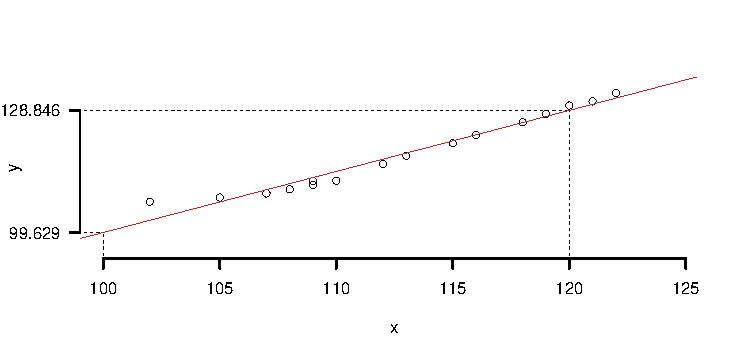
\includegraphics{Esami_passati_con_soluzioni_files/figure-latex/06-regr-48-1} \end{center}

\begin{eqnarray*}
\widehat{y} &=& -46.457 + 1.461 \,\times\, 100 = 99.629
                \qquad \mbox{per $x=100$} \qquad OY= 99.629 \\
\widehat{y} &=& -46.457 + 1.461 \,\times\, 120 = 128.846
                \qquad \mbox{per $x=120$} \qquad OY= 128.846\, .
\end{eqnarray*}

La ``piccola'' scala degli assi può portare a disegnare una retta
non appropriata; l'ispezione visiva aiuta, in questi casi, meglio
di quella numerica a disegnare una ``buona'' retta di regressione.

\end{sol}

1.d Fornire una interpretazione dei parametri della retta di regressione.

\begin{sol}
I parametri della retta di regressione sono \(\beta_{0}\) e \(\beta_{1}\).
Il primo, \(\beta_{0},\) rappresenta l'intercetta della retta, ovvero il
punto in cui la retta interseca l'asse delle ordinate.
Il secondo parametro, \(\beta_{1}\), rappresenta la pendenza della retta
(chiamato anche coefficiente angolare), ovvero l'incremento verticale
corrispondente a un incremento orizzontale unitario e coincide, perciò,
con la tangente dell'angolo compreso fra la retta e l'asse delle ascisse.

Quando si chiede di fornire una interpretazione dei parametri della retta
di regressione, tuttavia, si intende che il candidato interpreti anche
i valori numerici di \(\beta_{0}\) e \(\beta_{1}\) effettivamente calcolati
in precedenza, alla luce del fenomeno descritto da \(X\) e \(Y\).
In questo caso, l'indice della produzione industriale, secondo il modello
stimato, è dato da
\[y= -46.4575 + 1.4609 x\]
ossia, è composto da un quantitativo fisso di \(-46.4575\) quando l'indice
delle importazione è zero (\(X=0\)), un caso molto raro (ma impossibile
nel mondo attuale), a cui si aggiungono 1.4609 per ogni unità in più
dell'indice delle importazioni.

\end{sol}

1.e Calcolare un indicatore che sintetizzi l'ordine
di grandezza dei residui della retta di regressione.

\begin{sol}
La media quadratica dei residui della retta di regressione coincide con
il RMSE e rappresenta una sintesi della dispersione dei residui intorno
alla retta di regressione. Si calcola con la formula:

\begin{displaymath}
\hat\sigma_\varepsilon
= \sigma_{Y}\ \sqrt{1- r^2_{XY}} = 8.7462(1-0.9844^2) = 1.539
\end{displaymath}

\end{sol}

1.f Prevedere il valore dell'indice industriale per un valore
dell'indice delle importazioni pari a 120, ossia \(x=120\).

\begin{sol}
Si determina il valore previsto tramite la retta di regressione:

\begin{eqnarray*}
\widehat{Y}_{i}     &=& -46.4575 + 1.4609\times 120 \\
\widehat{y}_{x=120} &=& 128.8462
\end{eqnarray*}

\end{sol}

1.g Dal diagramma di dispersione sotto riportato,
spiegare se la retta di regressione è adeguata o no a
rappresentare il fenomeno.

\begin{center}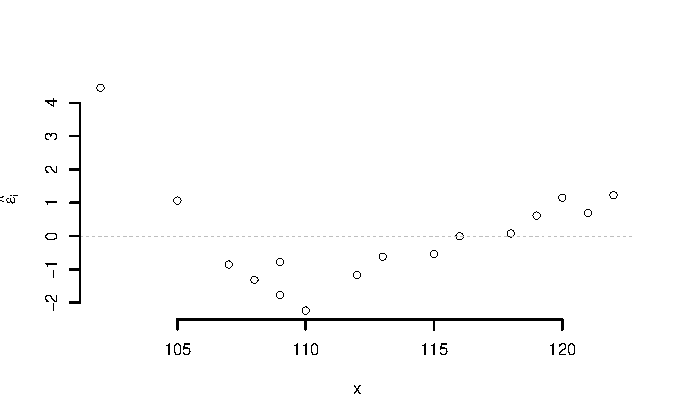
\includegraphics{Esami_passati_con_soluzioni_files/figure-latex/06-regr-50-1} \end{center}

\begin{sol}

L'ispezione visiva dei dati potrebbe suggerire anche l'esistenza
di una certa NON linearità.
Non vi sono punti leva; in ogni caso, la non linearità impone
di modellarla prima di cercare i punti leva.

\begin{center}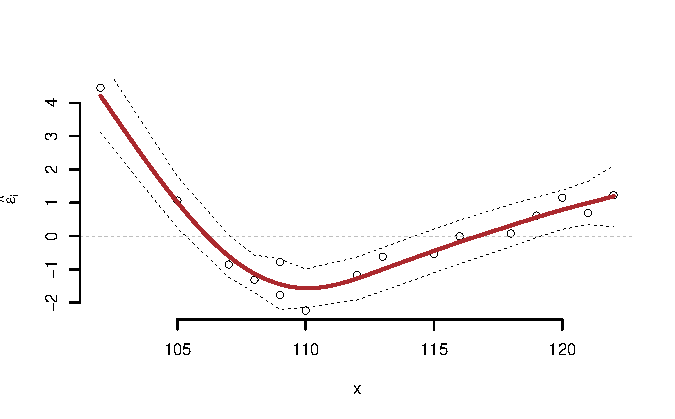
\includegraphics{Esami_passati_con_soluzioni_files/figure-latex/06-regr-51-1} \end{center}

\end{sol}

1.h Si consideri il diagramma dei residui sotto riportato.
Tracciare la retta dei residui.
Commentare la loro forma e spiegare se sono indipendenti o presentano
ancora una ``struttura'', un andamento peculiare.

\begin{sol}

La retta dei residui è parallela all'asse delle \(X\), ossia coincide con esso.
Il grafico dei residui evidenzia ancora la supposta la NON linearità;
infatti, i residui mostrano un andamento ``V'', tipica indicazione di
non linearità.

\begin{center}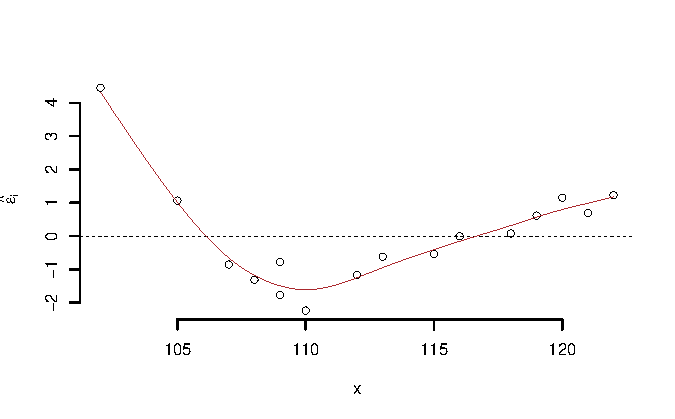
\includegraphics{Esami_passati_con_soluzioni_files/figure-latex/06-regr-53-1} \end{center}

\end{sol}

1.i\\
Verificare
l'ipotesi che la pendenza della retta di regressione sia uguale a
1 contro l'alternativa che sia maggiore di 1

\begin{sol}
\begin{eqnarray*}
\hat{\sigma_\varepsilon}^2&=&(1-r^2)\hat\sigma_Y^2\\
&=& (1- 0.969 )\times 76.5 \\
   &=&  2.369 \\
   S_\varepsilon^2 &=& \frac{n} {n-2} \hat{\sigma_\varepsilon}^2\\
   &=&  \frac{ 16 } { 16 -2} \hat{\sigma_\varepsilon}^2 \\
 &=&  \frac{ 16 } { 16 -2} \times  2.369  =  2.707  
\end{eqnarray*}

E quindi\begin{eqnarray*}
V(\hat\beta_{1}) &=& \frac{\sigma_{\varepsilon}^{2}} {n \hat{\sigma}^{2}_{X}} \\
\widehat{V(\hat\beta_{1})} &=& \frac{S_{\varepsilon}^{2}} {n \hat{\sigma}^{2}_{X}} \\
 &=& \frac{ 2.707 } { 16 \times  34.73 } =  0.004871 \\
 \widehat{SE(\hat\beta_{1})}        &=&  \sqrt{ 0.004871 }\\
 &=&  0.06979 
\end{eqnarray*}
\(\fbox{A}\) FORMULAZIONE DELLE IPOTESI

\[\begin{cases}
   H_0: \beta_1 = \beta_{1;H_0}=1 \\
   H_1: \beta_1 > \beta_{1;H_0}=1 
   \end{cases}\]

\(\fbox{B}\) SCELTA E CALCOLO STATISTICA-TEST, \(T\)
Test su un coefficiente di regressione: \(\Rightarrow\) t-Test.

\begin{eqnarray*}
 \frac{\hat\beta_{ 1 } - \beta_{ 1 ;H_0}} {\widehat{SE(\hat\beta_{ 1 })}}&\sim&t_{n-2}\\
   t_{\text{obs}}
&=& \frac{ ( 1.461 -  1 )} { 0.06979 }
 =   6.603 \, .
\end{eqnarray*}

\(\fbox{C}\) CONCLUSIONE

Consideriamo \(\alpha=0.1, 0.05, 0.01, 0.001\)

I valori critici sono

\(t_{16-2;0.1}=1.345\); \(t_{16-2;0.05}=1.7613\); \(t_{16-2;0.01}=2.6245\); \(t_{16-2;0.001}=3.7874\)

Siccome \(t_\text{obs}=6.6033>3.7874\), quindi \textbf{rifiuto} \(H_0\) sotto all'1‰,

\(p_\text{value}<0.001\), \emph{estremamente significativo} \(\fbox{***}\).

\begin{center}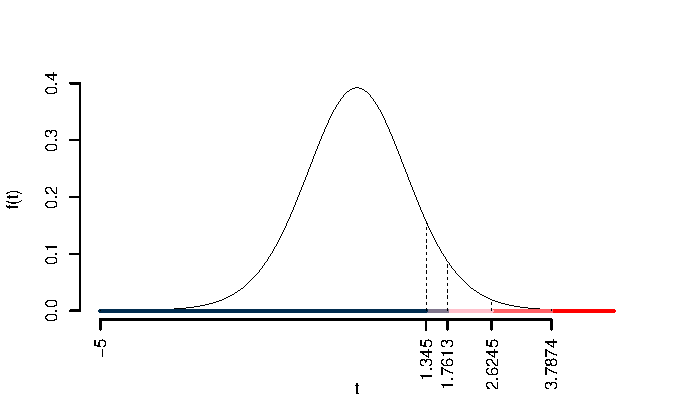
\includegraphics{Esami_passati_con_soluzioni_files/figure-latex/06-regr-7,-1} \end{center}

Il \(p_{\text{value}}\) è

\[ p_{\text{value}} = P(T_{16-2}>6.6)=0.000006 \]

Attenzione il calcolo del \(p_\text{value}\) con la \(T\) è puramente illustrativo e non può essere riprodotto senza una calcolatrice statistica adeguata.\[
 0 < p_\text{value}= 0.000006 \leq 0.001 
\]

\end{sol}

1.j Verificare l'ipotesi che l'intercetta della retta di
regressione sia uguale a zero contro l'alternativa che sia
minore di zero.

\begin{sol}
\begin{eqnarray*}
\hat{\sigma_\varepsilon}^2&=&(1-r^2)\hat\sigma_Y^2\\
&=& (1- 0.969 )\times 76.5 \\
   &=&  2.369 \\
   S_\varepsilon^2 &=& \frac{n} {n-2} \hat{\sigma_\varepsilon}^2\\
   &=&  \frac{ 16 } { 16 -2} \hat{\sigma_\varepsilon}^2 \\
 &=&  \frac{ 16 } { 16 -2} \times  2.369  =  2.707  
\end{eqnarray*}

E quindi\begin{eqnarray*}
V(\hat\beta_{0}) &=& \sigma_{\varepsilon}^{2} \left( \frac{1} {n}  +  \frac{\bar{x}^{2}} {n \hat{\sigma}^{2}_{X}} \right)\\
\widehat{V(\hat\beta_{0})} &=& S_{\varepsilon}^{2}\left( \frac{1} {n}  +  \frac{\bar{x}^{2}} {n \hat{\sigma}^{2}_{X}} \right)\ \\
 &=&  2.707 \times\left( \frac{1} { 16 }  +  \frac{ 112.9 ^{2}} { 16 \times  34.73 } \right)\\
 \widehat{SE(\hat\beta_{0})}        &=&  \sqrt{ 62.23 }\\
 &=&  7.889 
\end{eqnarray*}
\(\fbox{A}\) FORMULAZIONE DELLE IPOTESI

\[\begin{cases}
   H_0: \beta_0 = \beta_{0;H_0}=0 \\
   H_1: \beta_0 < \beta_{0;H_0}=0 
   \end{cases}\]

\(\fbox{B}\) SCELTA E CALCOLO STATISTICA-TEST, \(T\)
Test su un coefficiente di regressione: \(\Rightarrow\) t-Test.

\begin{eqnarray*}
 \frac{\hat\beta_{ 0 } - \beta_{ 0 ;H_0}} {\widehat{SE(\hat\beta_{ 0 })}}&\sim&t_{n-2}\\
   t_{\text{obs}}
&=& \frac{ ( -46.46 -  0 )} { 7.889 }
 =   -5.889 \, .
\end{eqnarray*}

\(\fbox{C}\) CONCLUSIONE

Consideriamo \(\alpha=0.1, 0.05, 0.01, 0.001\)

I valori critici sono

\(t_{16-2;0.1}=-1.345\); \(t_{16-2;0.05}=-1.7613\); \(t_{16-2;0.01}=-2.6245\); \(t_{16-2;0.001}=-3.7874\)

Siccome \(t_\text{obs}=-5.8892<-1.345\), quindi \textbf{rifiuto} \(H_0\) sotto all'1‰,

\(p_\text{value}<0.001\), \emph{estremamente significativo} \(\fbox{***}\).

\begin{center}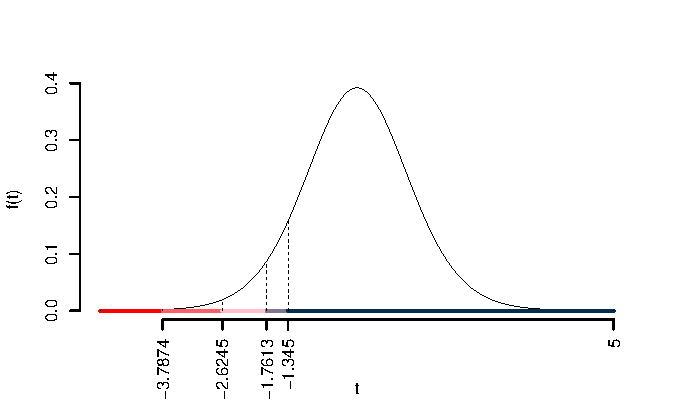
\includegraphics{Esami_passati_con_soluzioni_files/figure-latex/06-regr-8,-1} \end{center}

Il \(p_{\text{value}}\) è

\[ p_{\text{value}} = P(T_{16-2}<-5.89)=0.000020 \]

Attenzione il calcolo del \(p_\text{value}\) con la \(T\) è puramente illustrativo e non può essere riprodotto senza una calcolatrice statistica adeguata.\[
 0 < p_\text{value}= 0.000020 \leq 0.001 
\]

\end{sol}

\section{Esercizio 2}\label{esercizio-2-2}

Nella tabella seguente sono riportati i valori del seguente
esperimento: numero di ore dopo l'assunzione di un dato farmaco
(\(X\)) e incremento percentuale della pressione sistolica (\(Y\)).

\begin{table}[H]
\centering
\begin{tabular}{lrrrrrrrrrrr}
\toprule
$x$ & 0 & 1.00 & 2.00 & 3.0 & 4.00 & 5.00 & 6.00 & 7.00 & 8.00 & 9.00 & 10\\
$y$ & 10 & 1.42 & -0.53 & 2.6 & 4.02 & 4.49 & 5.72 & 6.54 & 8.91 & 8.74 & 0\\
\bottomrule
\end{tabular}
\end{table}

1.a Calcolare i parametri \(\beta_{0}\) e \(\beta_{1}\)
della retta di regressione in cui \(Y\) è spiegata attraverso \(X\).
(Suggerimento \(\bar{x} = 5\); \(\hat\sigma_{X} = 3.1623\);
\(\bar{y} = 4.7191\); \(\hat\sigma_{Y} = 3.4598\); \(\text{cov}(X,Y)= 1.5618\)).

\begin{sol}
\begin{eqnarray*}
       \hat\beta_1 &=& \frac{\text{cov}(X,Y)}{\hat\sigma_X^2} \\
            &=& \frac{ 1.562 }{ 10 }  =  0.1562 \\
      \hat\beta_0 &=& \bar y - \hat\beta_1 \bar x\\
          &=&  4.719 - 0.1562 \times  5 = 3.938 
      \end{eqnarray*}

\end{sol}

1.b Valutare la bontà di adattamento del modello precedente.

\begin{sol}
\begin{eqnarray*}
r&=&\frac{\text{cov}(X,Y)}{\sigma_X\sigma_Y}=\frac{ 1.562 }{ 3.162 \times 3.46 }= 0.1427 \\ 
r^2&=& 0.02038 < 0.75
\end{eqnarray*}

Il modello \textbf{non} si adatta bene ai dati.

Il modello spiega il \(2.04\%\) della variabilità totale della \(Y\).

\end{sol}

1.c Rappresentare nel diagramma di dispersione la retta di regressione.

\begin{sol}

Per disegnare velocemente la retta si individuano nel grafico
due punti: (1)il punto medio \((\bar{x},\, \bar{y})\), che è già
noto; e un solo punto ``estremo'' nel grafico, che può essere \(x=0\)
o \(x=10\) (i numeri ``tondi'' facilitano il calcolo e il disegno).
Qui, però, l'asse delle \(X\) presenta l'origine, ossia,
il valore \(x=0\) che ha come ordinata il valore di
\(\widehat{\beta_{0}}=3.9382\) già calcolato!
Diversamente, tramite l'equazione della retta di
regressione si stima la coordinata corrispondente:

\[\hat y_{X= 10 }=\hat\beta_0+\hat\beta_1 x= 3.938 + 0.1562 \times 10 = 5.5 \]

\begin{center}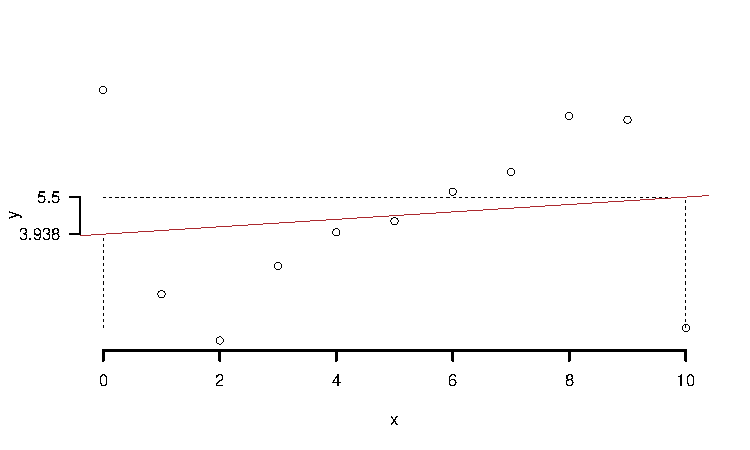
\includegraphics{Esami_passati_con_soluzioni_files/figure-latex/06-regr-54-1} \end{center}

\end{sol}

1.d Fornire una interpretazione dei parametri della retta di regressione.

\begin{sol}
I parametri della retta di regressione sono \(\beta_{0}\) e \(\beta_{1}\).
Il primo, \(\beta_{0},\) rappresenta l'intercetta della retta,
ovvero il punto in cui la retta interseca l'asse delle ordinate.
Il secondo parametro, \(\beta_{1}\), rappresenta la pendenza della
retta (chiamato anche coefficiente angolare), ovvero l'incremento
verticale corrispondente a un incremento orizzontale unitario e
coincide, perciò, con la tangente dell'angolo compreso fra la
retta e l'asse delle ascisse.

In questo caso, la variazione percentuale della pressione sistolica,
secondo il modello stimato, è dato da
\[Y= 3.9382 + 0.1562 X\]
ossia, è composta da un quantitativo fisso di \(3.9382\) che si ottiene
immediatamente dopo l'assunzione del farmaco (\(X=0\)), che non è privo
di significato, a cui si aggiunge un incremento di \(0.1562\) per ogni ora
aggiuntiva.

\end{sol}

1.e Prevedere il valore relativo a \(x=5\)
(notando che \(\bar{x}=5\), con opportune giustificazioni, si
può rispondere senza fare necessariamente i conti)

\begin{sol}
Dalle proprietà della retta di regressione si ha che:
\(\widehat{y}_{x=\bar{x}}=\bar{y}=4.7191\).
Ovvero: la retta di regressione passa per il punto \((\bar{x},\bar{y})\)

\end{sol}

1.f Calcolare l'ordine di grandezza dell'errore di previsione.

\begin{sol}
L'ordine di grandezza dell'errore di previsione commesso è dato
da RMSE che rappresenta una sintesi della dispersione dei residui
intorno alla retta di regressione.
\begin{displaymath}
\sigma_{\epsilon} = \sigma_{Y}\ \sqrt{1-r^2} = 3.4598 \sqrt{1-0.0204}
= 3.4244
\end{displaymath}

\end{sol}

1.g Verificare
l'ipotesi che la pendenza della retta di regressione sia uguale a
0 contro l'alternativa che sia diversa da 0

\begin{sol}
\begin{eqnarray*}
\hat{\sigma_\varepsilon}^2&=&(1-r^2)\hat\sigma_Y^2\\
&=& (1- 0.02038 )\times 11.97 \\
   &=&  11.73 \\
   S_\varepsilon^2 &=& \frac{n} {n-2} \hat{\sigma_\varepsilon}^2\\
   &=&  \frac{ 11 } { 11 -2} \hat{\sigma_\varepsilon}^2 \\
 &=&  \frac{ 11 } { 11 -2} \times  11.73  =  14.33  
\end{eqnarray*}

E quindi\begin{eqnarray*}
V(\hat\beta_{1}) &=& \frac{\sigma_{\varepsilon}^{2}} {n \hat{\sigma}^{2}_{X}} \\
\widehat{V(\hat\beta_{1})} &=& \frac{S_{\varepsilon}^{2}} {n \hat{\sigma}^{2}_{X}} \\
 &=& \frac{ 14.33 } { 11 \times  10 } =  0.1303 \\
 \widehat{SE(\hat\beta_{1})}        &=&  \sqrt{ 0.1303 }\\
 &=&  0.361 
\end{eqnarray*}

\(\fbox{A}\) FORMULAZIONE DELLE IPOTESI

\[\begin{cases}
   H_0: \beta_1 = \beta_{1;H_0}=0 \\
   H_1: \beta_1 \neq \beta_{1;H_0}=0 
   \end{cases}\]

\(\fbox{B}\) SCELTA E CALCOLO STATISTICA-TEST, \(T\)
Test su un coefficiente di regressione: \(\Rightarrow\) t-Test.

\begin{eqnarray*}
 \frac{\hat\beta_{ 1 } - \beta_{ 1 ;H_0}} {\widehat{SE(\hat\beta_{ 1 })}}&\sim&t_{n-2}\\
   t_{\text{obs}}
&=& \frac{ ( 0.1562 -  0 )} { 0.361 }
 =   0.4327 \, .
\end{eqnarray*}

\(\fbox{C}\) CONCLUSIONE

Siccome \(H_1\) è bilaterale, considereremo \(\alpha/2\),
anziché \(\alpha\)

\(\alpha=0.1, 0.05, 0.01, 0.001\) e quindi \(\alpha/2=0.05, 0.025, 0.005, 0.0005\)

I valori critici sono

\(t_{11-2;0.05}=1.8331\); \(t_{11-2;0.025}=2.2622\); \(t_{11-2;0.005}=3.2498\); \(t_{11-2;0.0005}=4.7809\)

Siccome \(|t_\text{obs}|=0.4327<t_{11-2;0.05}=1.8331\), quindi \textbf{non} rifiuto \(H_0\) a \textbf{nessun} livello di significatività,

\(p_\text{value}>0.1\), \emph{non significativo}

\begin{center}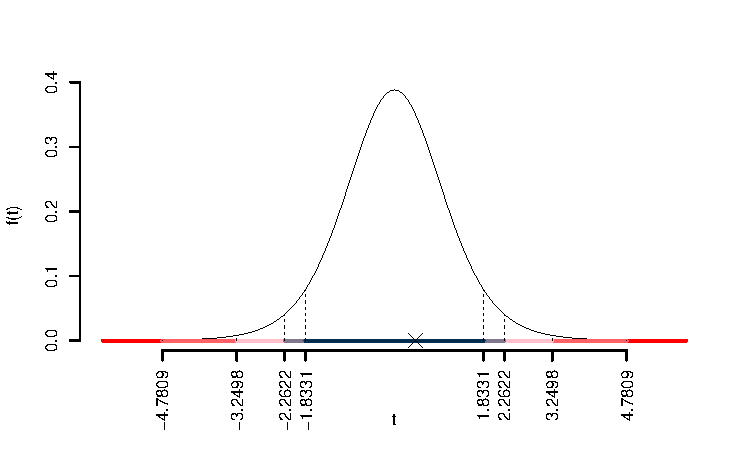
\includegraphics{Esami_passati_con_soluzioni_files/figure-latex/06-regr-13,-1} \end{center}

Il \(p_{\text{value}}\) è

\[ p_{\text{value}} = P(|T_{11-2}|>|0.43|)=2P(T_{11-2}>0.43)=0.675431 \]

Attenzione il calcolo del \(p_\text{value}\) con la \(T\) è puramente illustrativo e non può essere riprodotto senza una calcolatrice statistica adeguata.\[
 0.1 < p_\text{value}= 0.675431 \leq 1 
\]

\end{sol}

1.h\\
Verificare l'ipotesi che l'intercetta della retta di
regressione sia uguale a zero contro l'alternativa che sia
diversa da zero

\begin{sol}
\begin{eqnarray*}
\hat{\sigma_\varepsilon}^2&=&(1-r^2)\hat\sigma_Y^2\\
&=& (1- 0.02036 )\times 11.97 \\
   &=&  11.73 \\
   S_\varepsilon^2 &=& \frac{n} {n-2} \hat{\sigma_\varepsilon}^2\\
   &=&  \frac{ 11 } { 11 -2} \hat{\sigma_\varepsilon}^2 \\
 &=&  \frac{ 11 } { 11 -2} \times  11.73  =  14.33  
\end{eqnarray*}

E quindi\begin{eqnarray*}
V(\hat\beta_{0}) &=& \sigma_{\varepsilon}^{2} \left( \frac{1} {n}  +  \frac{\bar{x}^{2}} {n \hat{\sigma}^{2}_{X}} \right)\\
\widehat{V(\hat\beta_{0})} &=& S_{\varepsilon}^{2}\left( \frac{1} {n}  +  \frac{\bar{x}^{2}} {n \hat{\sigma}^{2}_{X}} \right)\ \\
 &=&  14.33 \times\left( \frac{1} { 11 }  +  \frac{ 5 ^{2}} { 11 \times  10 } \right)\\
 \widehat{SE(\hat\beta_{0})}        &=&  \sqrt{ 4.56 }\\
 &=&  2.135 
\end{eqnarray*}
\(\fbox{A}\) FORMULAZIONE DELLE IPOTESI

\[\begin{cases}
   H_0: \beta_0 = \beta_{0;H_0}=0 \\
   H_1: \beta_0 \neq \beta_{0;H_0}=0 
   \end{cases}\]

\(\fbox{B}\) SCELTA E CALCOLO STATISTICA-TEST, \(T\)
Test su un coefficiente di regressione: \(\Rightarrow\) t-Test.

\begin{eqnarray*}
 \frac{\hat\beta_{ 0 } - \beta_{ 0 ;H_0}} {\widehat{SE(\hat\beta_{ 0 })}}&\sim&t_{n-2}\\
   t_{\text{obs}}
&=& \frac{ ( 3.938 -  0 )} { 2.135 }
 =   1.844 \, .
\end{eqnarray*}

\(\fbox{C}\) CONCLUSIONE

Siccome \(H_1\) è bilaterale, considereremo \(\alpha/2\),
anziché \(\alpha\)

\(\alpha=0.1, 0.05, 0.01, 0.001\) e quindi \(\alpha/2=0.05, 0.025, 0.005, 0.0005\)

I valori critici sono

\(t_{11-2;0.05}=1.8331\); \(t_{11-2;0.025}=2.2622\); \(t_{11-2;0.005}=3.2498\); \(t_{11-2;0.0005}=4.7809\)

Siccome \(1.8331<|t_\text{obs}|=1.8442<2.2622\), indecisione sul rifiuto di \(H_0\) al 10\%,

\(0.05<p_\text{value}<0.1\), \emph{marginalmente significativo} \(\fbox{.}\).

\begin{center}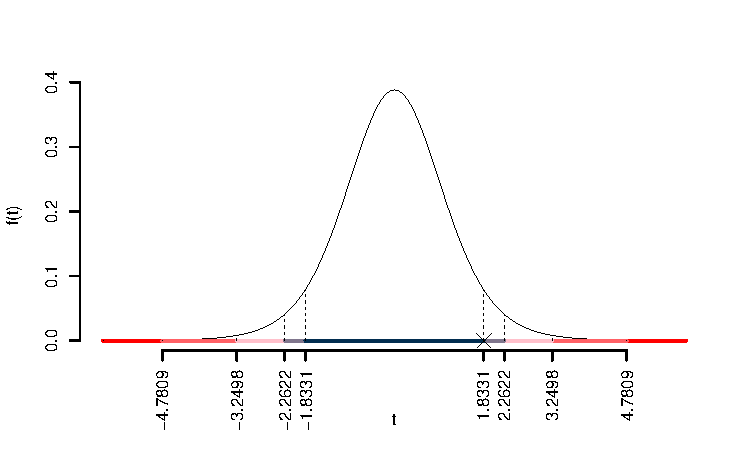
\includegraphics{Esami_passati_con_soluzioni_files/figure-latex/06-regr-14,-1} \end{center}

Il \(p_{\text{value}}\) è

\[ p_{\text{value}} = P(|T_{11-2}|>|1.84|)=2P(T_{11-2}>1.84)=0.098258 \]

Attenzione il calcolo del \(p_\text{value}\) con la \(T\) è puramente illustrativo e non può essere riprodotto senza una calcolatrice statistica adeguata.\[
 0.05 < p_\text{value}= 0.098258 \leq 0.1 
\]

\end{sol}

\section{Esercizio 3}\label{esercizio-3-1}

L'incasso settimanale di un negozio sia rappresentato dalla
variabile (casuale) \(X\) (in migliaia di euro).
L'uscita di cassa settimanale sia rappresentata dalla variabile
(casuale) \(Y\) (in migliaia di euro).
I dati rilevati per 4 mesi sono riportati di séguito.

\begin{table}[H]
\centering
\begin{tabular}{lrrrrrrrrrrrrrrrr}
\toprule
$x$ & 12 & 21 & 25 & 31 & 13 & 15 & 10 & 18 & 19 & 24 & 28 & 32 & 33 & 22 & 24 & 35\\
$y$ & 6 & 11 & 15 & 17 & 7 & 8 & 7 & 9 & 10 & 14 & 16 & 20 & 19 & 11 & 14 & 21\\
\bottomrule
\end{tabular}
\end{table}

1.a Calcolare i parametri \(\beta_{0}\) e \(\beta_{1}\)
della retta di regressione in cui \(Y\) è spiegata attraverso \(X\).
(Suggerimento \(\bar{x} = 22.625\); \(\hat\sigma_{X} = 7.5736\);
\(\bar{y} = 12.8125\); \(\hat\sigma_{Y} = 4.7331\); \(\text{cov}(X,Y)= 35.2422\)).

\begin{sol}
\begin{eqnarray*}
       \hat\beta_1 &=& \frac{\text{cov}(X,Y)}{\hat\sigma_X^2} \\
            &=& \frac{ 35.24 }{ 57.36 }  =  0.6144 \\
      \hat\beta_0 &=& \bar y - \hat\beta_1 \bar x\\
          &=&  12.81 - 0.6144 \times  22.625 = -1.089 
      \end{eqnarray*}

\end{sol}

1.b Valutare la bontà di adattamento del modello precedente.

\begin{sol}
\begin{eqnarray*}
r&=&\frac{\text{cov}(X,Y)}{\sigma_X\sigma_Y}=\frac{ 35.24 }{ 7.574 \times 4.733 }= 0.9831 \\ 
r^2&=& 0.9666 > 0.75
\end{eqnarray*}

Il modello si adatta bene ai dati.

Il modello spiega il \(96.66\%\) della variabilità totale della \(Y\).

\end{sol}

1.c Rappresentare nel diagramma di dispersione la retta di regressione.

\begin{sol}

Per disegnare velocemente la retta si individuano nel grafico
due punti: (1)il punto medio \((\bar{x},\, \bar{y})\), che è già
noto; e un solo punto ``estremo'' nel grafico, e un solo punto ``estremo'' nel grafico, che può essere \(x=5\) o
\(x=35\) (i numeri ``tondi'' facilitano il calcolo e il disegno, ma
qui \(x=0\) non funziona perché la Y diventa negativa). Tramite
l'equazione della retta di regressione si stima la coordinata
corrispondente:

\[\hat y_{X= 35 }=\hat\beta_0+\hat\beta_1 x= -1.089 + 0.6144 \times 35 = 20.42 \]

\begin{center}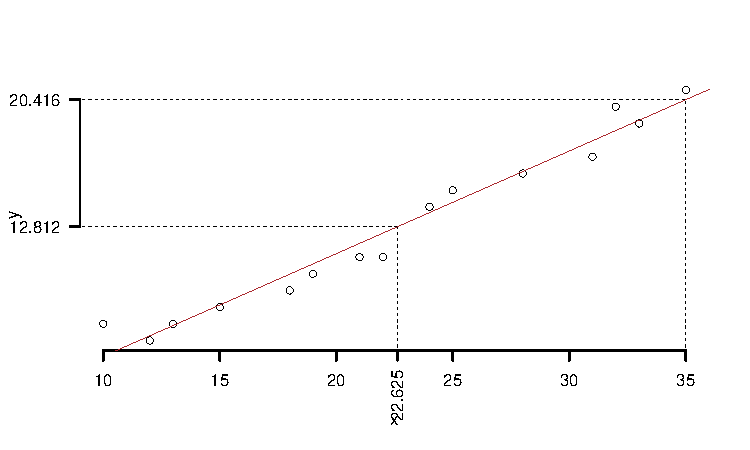
\includegraphics{Esami_passati_con_soluzioni_files/figure-latex/06-regr-55-1} \end{center}

\end{sol}

1.d Fornire una interpretazione dei parametri della retta di regressione.

\begin{sol}
I parametri della retta di regressione sono \(\beta_{0}\) e \(\beta_{1}\).
Il primo, \(\beta_{0},\) rappresenta l'intercetta della retta,
ovvero il punto in cui la retta interseca l'asse delle ordinate.
Il secondo parametro, \(\beta_{1}\), rappresenta la pendenza della
retta (chiamato anche coefficiente angolare), ovvero l'incremento
verticale corrispondente a un incremento orizzontale unitario e
coincide, perciò, con la tangente dell'angolo compreso fra la
retta e l'asse delle ascisse.

In questo caso, la variazione percentuale della pressione sistolica,
secondo il modello stimato, è dato da
\[Y= -1.0885 + 0.6144 X\]

ossia, è composta da un quantitativo fisso di \(-1.0885\) (migliaia
di euro) quando l'uscita di cassa è zero (\(X=0\)), a cui si
aggiungono \(0.6144\) migliaia di euro per ogni unità (in migliaia di
euro) di incasso aggiunto.

\end{sol}

1.e\\
Prevedere il valore dell'uscita per
un incasso di 30 migliaia di euro, ossia \(x=30\) e fornire l'ordine di grandezza dell'errore
di previsione commesso.

\begin{sol}
\[\hat y_{X= 30 }=\hat\beta_0+\hat\beta_1 x= -1.089 + 0.6144 \times 30 = 17.34 \]

\[
\hat\sigma_{\varepsilon}=\hat\sigma_Y\sqrt{1-r^2}=
4.7331\sqrt{1-0.9666}=0.8656
\]

\end{sol}

1.f Verificare
l'ipotesi che la pendenza della retta di regressione sia uguale a
1/2 contro l'alternativa che sia diversa da 1/2.

\begin{sol}
\begin{eqnarray*}
\hat{\sigma_\varepsilon}^2&=&(1-r^2)\hat\sigma_Y^2\\
&=& (1- 0.9666 )\times 22.4 \\
   &=&  0.7492 \\
   S_\varepsilon^2 &=& \frac{n} {n-2} \hat{\sigma_\varepsilon}^2\\
   &=&  \frac{ 16 } { 16 -2} \hat{\sigma_\varepsilon}^2 \\
 &=&  \frac{ 16 } { 16 -2} \times  0.7492  =  0.8562  
\end{eqnarray*}

E quindi\begin{eqnarray*}
V(\hat\beta_{1}) &=& \frac{\sigma_{\varepsilon}^{2}} {n \hat{\sigma}^{2}_{X}} \\
\widehat{V(\hat\beta_{1})} &=& \frac{S_{\varepsilon}^{2}} {n \hat{\sigma}^{2}_{X}} \\
 &=& \frac{ 0.8562 } { 16 \times  57.36 } =  0.0009329 \\
 \widehat{SE(\hat\beta_{1})}        &=&  \sqrt{ 0.0009329 }\\
 &=&  0.03054 
\end{eqnarray*}

\(\fbox{A}\) FORMULAZIONE DELLE IPOTESI

\[\begin{cases}
   H_0: \beta_1 = \beta_{1;H_0}=0.5 \\
   H_1: \beta_1 \neq \beta_{1;H_0}=0.5 
   \end{cases}\]

\(\fbox{B}\) SCELTA E CALCOLO STATISTICA-TEST, \(T\)
Test su un coefficiente di regressione: \(\Rightarrow\) t-Test.

\begin{eqnarray*}
 \frac{\hat\beta_{ 1 } - \beta_{ 1 ;H_0}} {\widehat{SE(\hat\beta_{ 1 })}}&\sim&t_{n-2}\\
   t_{\text{obs}}
&=& \frac{ ( 0.6144 -  0.5 )} { 0.03054 }
 =   3.746 \, .
\end{eqnarray*}

\(\fbox{C}\) CONCLUSIONE

Siccome \(H_1\) è bilaterale, considereremo \(\alpha/2\),
anziché \(\alpha\)

\(\alpha=0.1, 0.05, 0.01, 0.001\) e quindi \(\alpha/2=0.05, 0.025, 0.005, 0.0005\)

I valori critici sono

\(t_{16-2;0.05}=1.7613\); \(t_{16-2;0.025}=2.1448\); \(t_{16-2;0.005}=2.9768\); \(t_{16-2;0.0005}=4.1405\)

Siccome \(2.9768<|t_\text{obs}|=3.7457<4.1405\), quindi \textbf{rifiuto} \(H_0\) all'1\%,

\(0.001<p_\text{value}<0.01\), \emph{molto significativo} \(\fbox{**}\).

\begin{center}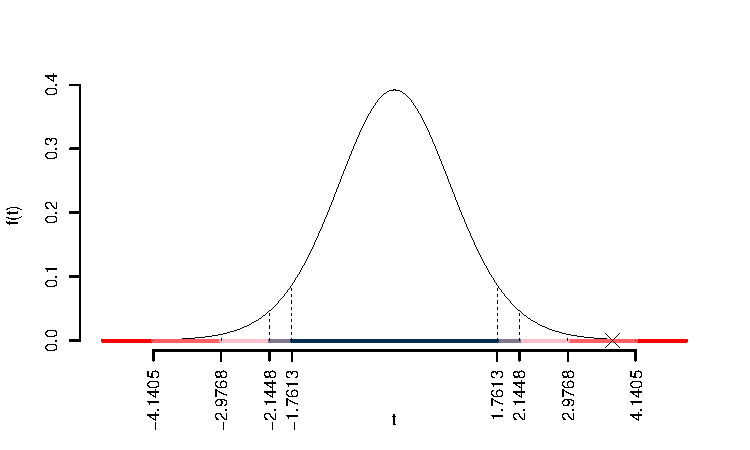
\includegraphics{Esami_passati_con_soluzioni_files/figure-latex/06-regr-20,-1} \end{center}

Il \(p_{\text{value}}\) è

\[ p_{\text{value}} = P(|T_{16-2}|>|3.75|)=2P(T_{16-2}>3.75)=0.002172 \]

Attenzione il calcolo del \(p_\text{value}\) con la \(T\) è puramente illustrativo e non può essere riprodotto senza una calcolatrice statistica adeguata.\[
 0.001 < p_\text{value}= 0.002172 \leq 0.01 
\]

\end{sol}

1.g\\
Verificare l'ipotesi che l'intercetta della retta di
regressione sia uguale a zero contro l'alternativa che sia
minore di zero.

\begin{sol}
\begin{eqnarray*}
\hat{\sigma_\varepsilon}^2&=&(1-r^2)\hat\sigma_Y^2\\
&=& (1- 0.9665 )\times 22.4 \\
   &=&  0.7492 \\
   S_\varepsilon^2 &=& \frac{n} {n-2} \hat{\sigma_\varepsilon}^2\\
   &=&  \frac{ 16 } { 16 -2} \hat{\sigma_\varepsilon}^2 \\
 &=&  \frac{ 16 } { 16 -2} \times  0.7492  =  0.8562  
\end{eqnarray*}

E quindi\begin{eqnarray*}
V(\hat\beta_{0}) &=& \sigma_{\varepsilon}^{2} \left( \frac{1} {n}  +  \frac{\bar{x}^{2}} {n \hat{\sigma}^{2}_{X}} \right)\\
\widehat{V(\hat\beta_{0})} &=& S_{\varepsilon}^{2}\left( \frac{1} {n}  +  \frac{\bar{x}^{2}} {n \hat{\sigma}^{2}_{X}} \right)\ \\
 &=&  0.8562 \times\left( \frac{1} { 16 }  +  \frac{ 22.62 ^{2}} { 16 \times  57.36 } \right)\\
 \widehat{SE(\hat\beta_{0})}        &=&  \sqrt{ 0.5311 }\\
 &=&  0.7288 
\end{eqnarray*}
\(\fbox{A}\) FORMULAZIONE DELLE IPOTESI

\[\begin{cases}
   H_0: \beta_0 = \beta_{0;H_0}=0 \\
   H_1: \beta_0 < \beta_{0;H_0}=0 
   \end{cases}\]

\(\fbox{B}\) SCELTA E CALCOLO STATISTICA-TEST, \(T\)
Test su un coefficiente di regressione: \(\Rightarrow\) t-Test.

\begin{eqnarray*}
 \frac{\hat\beta_{ 0 } - \beta_{ 0 ;H_0}} {\widehat{SE(\hat\beta_{ 0 })}}&\sim&t_{n-2}\\
   t_{\text{obs}}
&=& \frac{ ( -1.089 -  0 )} { 0.7288 }
 =   -1.494 \, .
\end{eqnarray*}

\(\fbox{C}\) CONCLUSIONE

Consideriamo \(\alpha=0.1, 0.05, 0.01, 0.001\)

I valori critici sono

\(t_{16-2;0.1}=-1.345\); \(t_{16-2;0.05}=-1.7613\); \(t_{16-2;0.01}=-2.6245\); \(t_{16-2;0.001}=-3.7874\)

Siccome \(-3.7874<t_\text{obs}=-1.4936<-2.6245\), indecisione sul rifiuto di \(H_0\) al 10\%,

\(0.05<p_\text{value}<0.1\), \emph{marginalmente significativo} \(\fbox{.}\).

\begin{center}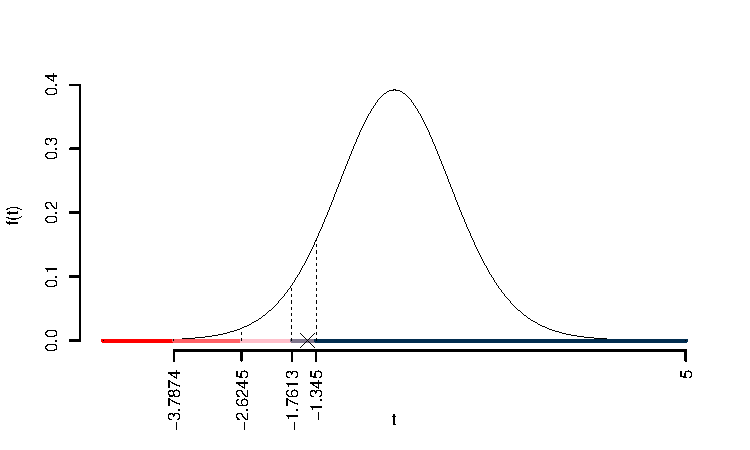
\includegraphics{Esami_passati_con_soluzioni_files/figure-latex/06-regr-21,-1} \end{center}

Il \(p_{\text{value}}\) è

\[ p_{\text{value}} = P(T_{16-2}<-1.49)=0.078734 \]

Attenzione il calcolo del \(p_\text{value}\) con la \(T\) è puramente illustrativo e non può essere riprodotto senza una calcolatrice statistica adeguata.\[
 0.05 < p_\text{value}= 0.078734 \leq 0.1 
\]

\end{sol}

\section{Esercizio 4}\label{esercizio-4-1}

Si esaminano 15 aziende e si rileva, per ognuna di esse,
il numero di addetti (\(X\)) e il fatturato (\(Y\) in unità
convenzionali).
I risultati sono riportati nella tabella seguente.

\begin{table}[H]
\centering
\begin{tabular}{lrrrrrrrrrrrrrrr}
\toprule
$x$ & 20 & 30 & 40 & 50 & 60 & 70 & 80 & 90 & 100 & 110 & 120 & 130 & 140 & 150 & 160\\
$y$ & 25 & 40 & 50 & 64 & 75 & 85 & 100 & 105 & 120 & 145 & 178 & 210 & 260 & 315 & 380\\
\bottomrule
\end{tabular}
\end{table}

1.a Calcolare i parametri \(\beta_{0}\) e \(\beta_{1}\)
della retta di regressione in cui \(Y\) è spiegata attraverso \(X\).
(Suggerimento \(\bar{x} = 90\); \(\hat\sigma_{X} = 43.2049\);
\(\bar{y} = 143.4667\); \(\hat\sigma_{Y} = 102.1077\); \(\text{cov}(X,Y)= 4145.3333\)).

\begin{sol}
\begin{eqnarray*}
       \hat\beta_1 &=& \frac{\text{cov}(X,Y)}{\hat\sigma_X^2} \\
            &=& \frac{ 4145 }{ 1867 }  =  2.221 \\
      \hat\beta_0 &=& \bar y - \hat\beta_1 \bar x\\
          &=&  143.5 - 2.2207 \times  90 = -56.4 
      \end{eqnarray*}

\end{sol}

1.b Valutare la bontà di adattamento del modello precedente.

\begin{sol}
\begin{eqnarray*}
r&=&\frac{\text{cov}(X,Y)}{\sigma_X\sigma_Y}=\frac{ 4145 }{ 43.2 \times 102.1 }= 0.9397 \\ 
r^2&=& 0.8829 > 0.75
\end{eqnarray*}

Il modello si adatta bene ai dati.

Il modello spiega il \(88.29\%\) della variabilità totale della \(Y\).

\end{sol}

1.c Rappresentare nel diagramma di dispersione la retta di regressione.

\begin{sol}

Per disegnare velocemente la retta si individuano nel grafico
due punti: (1)il punto medio \((\bar{x},\, \bar{y})\), che è già
noto; e un solo punto ``estremo'' nel grafico, e un solo punto ``estremo'' nel
nel grafico, che può essere \(x=160\)
o \(x=40\) (un numero inferiore dà un \(y\) negativo).
Quest'ultimo NON conviene perché ``esce'' dagli assi.
Tramite l'equazione della retta di regressione si stima la coordinata
corrispondente:

\[\hat y_{X= 40 }=\hat\beta_0+\hat\beta_1 x= -56.4 + 2.2207 \times 40 = 32.43 \]

\begin{center}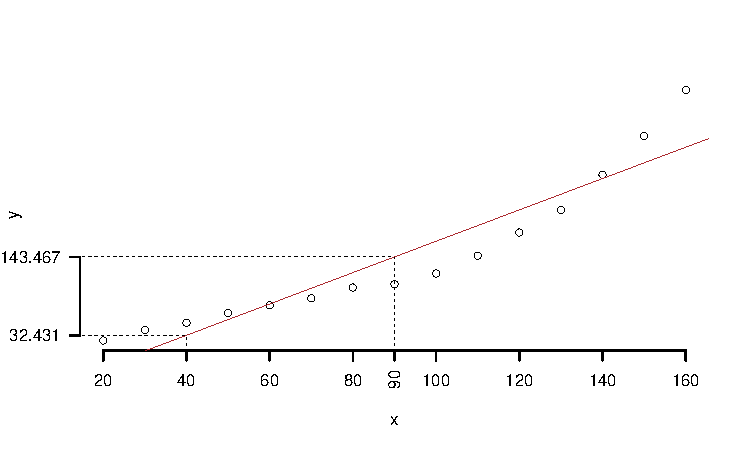
\includegraphics{Esami_passati_con_soluzioni_files/figure-latex/06-regr-56-1} \end{center}

\end{sol}

1.d Fornire una interpretazione dei parametri della retta di regressione.

\begin{sol}
I parametri della retta di regressione sono \(\beta_{0}\) e \(\beta_{1}\).
Il primo, \(\beta_{0},\) rappresenta l'intercetta della retta,
ovvero il punto in cui la retta interseca l'asse delle ordinate.
Il secondo parametro, \(\beta_{1}\), rappresenta la pendenza della
retta (chiamato anche coefficiente angolare), ovvero l'incremento
verticale corrispondente a un incremento orizzontale unitario e
coincide, perciò, con la tangente dell'angolo compreso fra la
retta e l'asse delle ascisse.

In questo caso, il numero di addetti, secondo il modello stimato,
è dato da
\[y= -56.3976 + 2.2207 x\]
ossia, è composto da un quantitativo fisso di \(-56.3976\)
di fatturato quando il numero degli addetti è è zero (\(X=0\))
che corrisponde al costo di una impresa senza addetti, a cui
si aggiungono 2.2207 per ogni unità di lavoro aggiuntiva.

\end{sol}

1.e Prevedere il valore del fatturato per un numero
di addetti pari a 75 unità, ossia per \(x=75\).

\begin{sol}
\[\hat y_{X= 75 }=\hat\beta_0+\hat\beta_1 x= -56.4 + 2.2207 \times 75 = 110.2 \]

\end{sol}

1.f Verificare
l'ipotesi che la pendenza della retta di regressione sia uguale a
2 contro l'alternativa che sia maggiore di 2, sapendo che

\begin{sol}
\begin{eqnarray*}
\hat{\sigma_\varepsilon}^2&=&(1-r^2)\hat\sigma_Y^2\\
&=& (1- 0.8829 )\times 10426 \\
   &=&  1220 \\
   S_\varepsilon^2 &=& \frac{n} {n-2} \hat{\sigma_\varepsilon}^2\\
   &=&  \frac{ 15 } { 15 -2} \hat{\sigma_\varepsilon}^2 \\
 &=&  \frac{ 15 } { 15 -2} \times  1220  =  1408  
\end{eqnarray*}

E quindi\begin{eqnarray*}
V(\hat\beta_{1}) &=& \frac{\sigma_{\varepsilon}^{2}} {n \hat{\sigma}^{2}_{X}} \\
\widehat{V(\hat\beta_{1})} &=& \frac{S_{\varepsilon}^{2}} {n \hat{\sigma}^{2}_{X}} \\
 &=& \frac{ 1408 } { 15 \times  1867 } =  0.05029 \\
 \widehat{SE(\hat\beta_{1})}        &=&  \sqrt{ 0.05029 }\\
 &=&  0.2243 
\end{eqnarray*}

\(\fbox{A}\) FORMULAZIONE DELLE IPOTESI

\[\begin{cases}
   H_0: \beta_1 = \beta_{1;H_0}=2 \\
   H_1: \beta_1 > \beta_{1;H_0}=2 
   \end{cases}\]

\(\fbox{B}\) SCELTA E CALCOLO STATISTICA-TEST, \(T\)
Test su un coefficiente di regressione: \(\Rightarrow\) t-Test.

\begin{eqnarray*}
 \frac{\hat\beta_{ 1 } - \beta_{ 1 ;H_0}} {\widehat{SE(\hat\beta_{ 1 })}}&\sim&t_{n-2}\\
   t_{\text{obs}}
&=& \frac{ ( 2.221 -  2 )} { 0.2243 }
 =   0.9842 \, .
\end{eqnarray*}

\(\fbox{C}\) CONCLUSIONE

Consideriamo \(\alpha=0.1, 0.05, 0.01, 0.001\)

I valori critici sono

\(t_{15-2;0.1}=1.3502\); \(t_{15-2;0.05}=1.7709\); \(t_{15-2;0.01}=2.6503\); \(t_{15-2;0.001}=3.852\)

Siccome \(t_\text{obs}=0.9842<t_{15-2;0.1}=1.3502\), quindi \textbf{non} rifiuto \(H_0\) a \textbf{nessun} livello di significatività,

\(p_\text{value}>0.1\), \emph{non significativo}

\begin{center}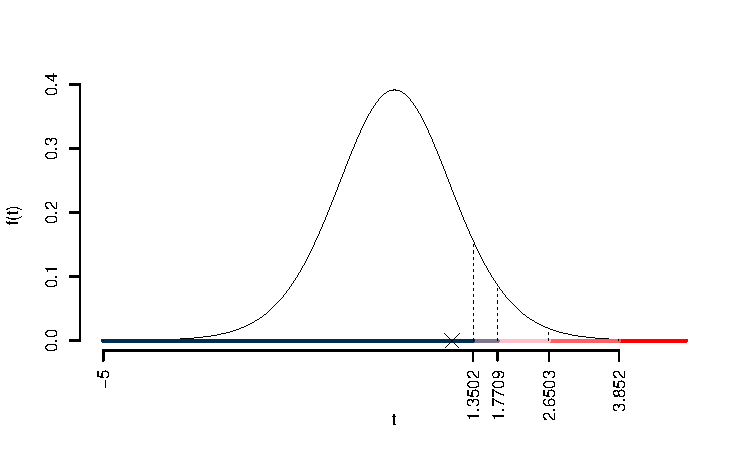
\includegraphics{Esami_passati_con_soluzioni_files/figure-latex/06-regr-27,-1} \end{center}

Il \(p_{\text{value}}\) è

\[ p_{\text{value}} = P(T_{15-2}>0.98)=0.171488 \]

Attenzione il calcolo del \(p_\text{value}\) con la \(T\) è puramente illustrativo e non può essere riprodotto senza una calcolatrice statistica adeguata.\[
 0.1 < p_\text{value}= 0.171488 \leq 1 
\]

\end{sol}

1.g\\
Verificare l'ipotesi che l'intercetta della retta di
regressione sia uguale a zero contro l'alternativa che sia
minore di zero.

\begin{sol}
\begin{eqnarray*}
\hat{\sigma_\varepsilon}^2&=&(1-r^2)\hat\sigma_Y^2\\
&=& (1- 0.883 )\times 10426 \\
   &=&  1220 \\
   S_\varepsilon^2 &=& \frac{n} {n-2} \hat{\sigma_\varepsilon}^2\\
   &=&  \frac{ 15 } { 15 -2} \hat{\sigma_\varepsilon}^2 \\
 &=&  \frac{ 15 } { 15 -2} \times  1220  =  1408  
\end{eqnarray*}

E quindi\begin{eqnarray*}
V(\hat\beta_{0}) &=& \sigma_{\varepsilon}^{2} \left( \frac{1} {n}  +  \frac{\bar{x}^{2}} {n \hat{\sigma}^{2}_{X}} \right)\\
\widehat{V(\hat\beta_{0})} &=& S_{\varepsilon}^{2}\left( \frac{1} {n}  +  \frac{\bar{x}^{2}} {n \hat{\sigma}^{2}_{X}} \right)\ \\
 &=&  1408 \times\left( \frac{1} { 15 }  +  \frac{ 90 ^{2}} { 15 \times  1867 } \right)\\
 \widehat{SE(\hat\beta_{0})}        &=&  \sqrt{ 501.2 }\\
 &=&  22.39 
\end{eqnarray*}
\(\fbox{A}\) FORMULAZIONE DELLE IPOTESI

\[\begin{cases}
   H_0: \beta_0 = \beta_{0;H_0}=0 \\
   H_1: \beta_0 < \beta_{0;H_0}=0 
   \end{cases}\]

\(\fbox{B}\) SCELTA E CALCOLO STATISTICA-TEST, \(T\)
Test su un coefficiente di regressione: \(\Rightarrow\) t-Test.

\begin{eqnarray*}
 \frac{\hat\beta_{ 0 } - \beta_{ 0 ;H_0}} {\widehat{SE(\hat\beta_{ 0 })}}&\sim&t_{n-2}\\
   t_{\text{obs}}
&=& \frac{ ( -56.4 -  0 )} { 22.39 }
 =   -2.519 \, .
\end{eqnarray*}

\(\fbox{C}\) CONCLUSIONE

Consideriamo \(\alpha=0.1, 0.05, 0.01, 0.001\)

I valori critici sono

\(t_{15-2;0.1}=-1.3502\); \(t_{15-2;0.05}=-1.7709\); \(t_{15-2;0.01}=-2.6503\); \(t_{15-2;0.001}=-3.852\)

Siccome \(-2.6503<t_\text{obs}=-2.5191<-1.7709\), quindi \textbf{rifiuto} \(H_0\) al 5\%,

\(0.01<p_\text{value}<0.05\), \emph{significativo} \(\fbox{*}\).

\begin{center}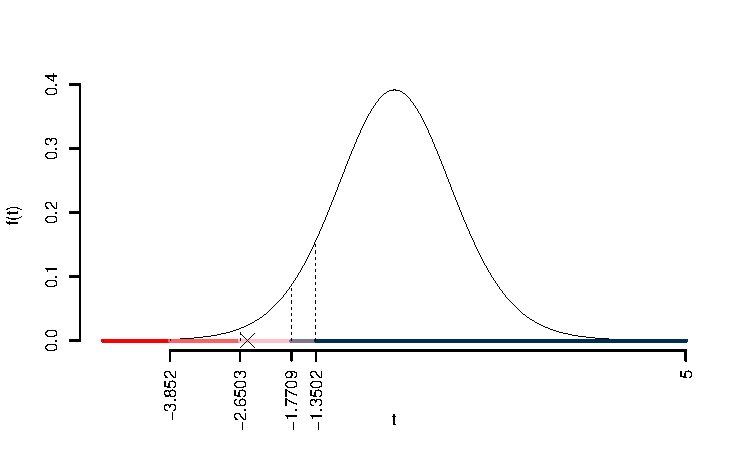
\includegraphics{Esami_passati_con_soluzioni_files/figure-latex/06-regr-28,-1} \end{center}

Il \(p_{\text{value}}\) è

\[ p_{\text{value}} = P(T_{15-2}<-2.52)=0.012824 \]

Attenzione il calcolo del \(p_\text{value}\) con la \(T\) è puramente illustrativo e non può essere riprodotto senza una calcolatrice statistica adeguata.\[
 0.01 < p_\text{value}= 0.012824 \leq 0.05 
\]

\end{sol}

\section{Esercizio 5}\label{esercizio-5}

Nel maggio del 1973 per 15 giorni consecutivi si sono osservati i valori
di concentrazione di ozono (espressa in parti per milione) a New York \(Y\)
e temperatura a terra, \(X\) (espressa in gradi Fahrenheit), come espresso
nella seguente tabella.

\begin{table}[H]
\centering
\begin{tabular}{lrrrrrrrrrrrrrrr}
\toprule
$x$ & 20 & 30 & 40 & 50 & 60 & 70 & 80 & 90 & 100 & 110 & 120 & 130 & 140 & 150 & 160\\
$y$ & 25 & 40 & 50 & 64 & 75 & 85 & 100 & 105 & 120 & 145 & 178 & 210 & 260 & 315 & 380\\
\bottomrule
\end{tabular}
\end{table}

1.a Calcolare i parametri \(\beta_{0}\) e \(\beta_{1}\)
della retta di regressione in cui \(Y\) è spiegata attraverso \(X\).
(Suggerimento \(\bar{x} = 90\); \(\hat\sigma_{X} = 43.2049\);
\(\bar{y} = 143.4667\); \(\hat\sigma_{Y} = 102.1077\); \(\text{cov}(X,Y)= 4145.3333\)).

\begin{sol}
\begin{eqnarray*}
       \hat\beta_1 &=& \frac{\text{cov}(X,Y)}{\hat\sigma_X^2} \\
            &=& \frac{ 4145 }{ 1867 }  =  2.221 \\
      \hat\beta_0 &=& \bar y - \hat\beta_1 \bar x\\
          &=&  143.5 - 2.2207 \times  90 = -56.4 
      \end{eqnarray*}

\end{sol}

1.b Valutare la bontà di adattamento del modello precedente.

\begin{sol}
\begin{eqnarray*}
r&=&\frac{\text{cov}(X,Y)}{\sigma_X\sigma_Y}=\frac{ 4145 }{ 43.2 \times 102.1 }= 0.9397 \\ 
r^2&=& 0.8829 > 0.75
\end{eqnarray*}

Il modello si adatta bene ai dati.

Il modello spiega il \(88.29\%\) della variabilità totale della \(Y\).

\end{sol}

\textbf{Nota} altre domande simili alle precedenti non vengono riportate

1.c\\
Verificare l'ipotesi che l'intercetta della retta di
regressione sia uguale a zero contro l'alternativa che sia
minore di zero.

\begin{sol}
\begin{eqnarray*}
\hat{\sigma_\varepsilon}^2&=&(1-r^2)\hat\sigma_Y^2\\
&=& (1- 0.8829 )\times 10426 \\
   &=&  1220 \\
   S_\varepsilon^2 &=& \frac{n} {n-2} \hat{\sigma_\varepsilon}^2\\
   &=&  \frac{ 15 } { 15 -2} \hat{\sigma_\varepsilon}^2 \\
 &=&  \frac{ 15 } { 15 -2} \times  1220  =  1408  
\end{eqnarray*}

E quindi\begin{eqnarray*}
V(\hat\beta_{0}) &=& \sigma_{\varepsilon}^{2} \left( \frac{1} {n}  +  \frac{\bar{x}^{2}} {n \hat{\sigma}^{2}_{X}} \right)\\
\widehat{V(\hat\beta_{0})} &=& S_{\varepsilon}^{2}\left( \frac{1} {n}  +  \frac{\bar{x}^{2}} {n \hat{\sigma}^{2}_{X}} \right)\ \\
 &=&  1408 \times\left( \frac{1} { 15 }  +  \frac{ 90 ^{2}} { 15 \times  1867 } \right)\\
 \widehat{SE(\hat\beta_{0})}        &=&  \sqrt{ 501.2 }\\
 &=&  22.39 
\end{eqnarray*}
\(\fbox{A}\) FORMULAZIONE DELLE IPOTESI

\[\begin{cases}
   H_0: \beta_0 = \beta_{0;H_0}=0 \\
   H_1: \beta_0 < \beta_{0;H_0}=0 
   \end{cases}\]

\(\fbox{B}\) SCELTA E CALCOLO STATISTICA-TEST, \(T\)
Test su un coefficiente di regressione: \(\Rightarrow\) t-Test.

\begin{eqnarray*}
 \frac{\hat\beta_{ 0 } - \beta_{ 0 ;H_0}} {\widehat{SE(\hat\beta_{ 0 })}}&\sim&t_{n-2}\\
   t_{\text{obs}}
&=& \frac{ ( -56.4 -  0 )} { 22.39 }
 =   -2.519 \, .
\end{eqnarray*}

\(\fbox{C}\) CONCLUSIONE

Consideriamo \(\alpha=0.1, 0.05, 0.01, 0.001\)

I valori critici sono

\(t_{15-2;0.1}=-1.3502\); \(t_{15-2;0.05}=-1.7709\); \(t_{15-2;0.01}=-2.6503\); \(t_{15-2;0.001}=-3.852\)

Siccome \(-2.6503<t_\text{obs}=-2.5191<-1.7709\), quindi \textbf{rifiuto} \(H_0\) al 5\%,

\(0.01<p_\text{value}<0.05\), \emph{significativo} \(\fbox{*}\).

\begin{center}\includegraphics{Esami_passati_con_soluzioni_files/figure-latex/06-regr-32,-1} \end{center}

Il \(p_{\text{value}}\) è

\[ p_{\text{value}} = P(T_{15-2}<-2.52)=0.012824 \]

Attenzione il calcolo del \(p_\text{value}\) con la \(T\) è puramente illustrativo e non può essere riprodotto senza una calcolatrice statistica adeguata.\[
 0.01 < p_\text{value}= 0.012824 \leq 0.05 
\]

\end{sol}

\section{Esercizio 6}\label{esercizio-6}

Il reddito pro capite, in migliaia di euro, relativo a 16 aree
amministrative rilevato nell'anno 1989, \(X\), e rilevato nell'anno
1999, \(Y\), sono riportati nella tabella seguente.

\footnotesize
\begin{table}[H]
\centering
\begin{tabular}{lrrrrrrrrrrrrrrrr}
\toprule
$x$ & 47.8 & 27.9 & 36.6 & 54.2 & 41.9 & 44.4 & 54.3 & 42.3 & 41.5 & 43.2 & 56.3 & 63.3 & 46.8 & 45.2 & 38.7 & 36.3\\
$y$ & 63.0 & 33.4 & 42.0 & 72.8 & 52.0 & 54.0 & 63.4 & 60.7 & 54.4 & 55.5 & 74.0 & 79.2 & 53.1 & 59.6 & 52.0 & 47.2\\
\bottomrule
\end{tabular}
\end{table}
\normalsize

1.a Calcolare i parametri \(\beta_{0}\) e \(\beta_{1}\)
della retta di regressione in cui \(Y\) è spiegata attraverso \(X\).
(Suggerimento \(\bar{x} = 45.0438\); \(\hat\sigma_{X} = 8.4996\);
\(\bar{y} = 57.2687\); \(\hat\sigma_{Y} = 11.4263\); \(\text{cov}(X,Y)= 92.4239\)).

\begin{sol}
\begin{eqnarray*}
       \hat\beta_1 &=& \frac{\text{cov}(X,Y)}{\hat\sigma_X^2} \\
            &=& \frac{ 92.42 }{ 72.24 }  =  1.279 \\
      \hat\beta_0 &=& \bar y - \hat\beta_1 \bar x\\
          &=&  57.27 - 1.2793 \times  45.0438 = -0.3573 
      \end{eqnarray*}

\end{sol}

1.b Valutare la bontà di adattamento del modello precedente.

\begin{sol}
\begin{eqnarray*}
r&=&\frac{\text{cov}(X,Y)}{\sigma_X\sigma_Y}=\frac{ 92.42 }{ 8.5 \times 11.43 }= 0.9517 \\ 
r^2&=& 0.9056 > 0.75
\end{eqnarray*}

Il modello si adatta bene ai dati.

Il modello spiega il \(90.56\%\) della variabilità totale della \(Y\).

\end{sol}

1.c Determinare il residuo (o l'errore) derivante
dalla previsione, calcolata con il modello di regressione in \(x=54.3\).

\begin{sol}
\begin{eqnarray*}
\hat y_i &=&\hat\beta_0+\hat\beta_1 x_i=\\ 
&=& -0.3573 + 1.2793 \times 54.3 = 69.11 \\ 
\hat \varepsilon_i &=& y_i-\hat y_i\\ 
&=& 63.4 - 69.1106 = -5.711  
\end{eqnarray*}

\end{sol}

\textbf{Nota} altre domande simili alle precedenti non vengono riportate

1.d\\
Verificare
l'ipotesi che la pendenza della retta di regressione sia uguale a 0
contro l'alternativa che sia maggiore di 0.

\begin{sol}
\begin{eqnarray*}
\hat{\sigma_\varepsilon}^2&=&(1-r^2)\hat\sigma_Y^2\\
&=& (1- 0.9056 )\times 130.6 \\
   &=&  12.32 \\
   S_\varepsilon^2 &=& \frac{n} {n-2} \hat{\sigma_\varepsilon}^2\\
   &=&  \frac{ 16 } { 16 -2} \hat{\sigma_\varepsilon}^2 \\
 &=&  \frac{ 16 } { 16 -2} \times  12.32  =  14.08  
\end{eqnarray*}

E quindi\begin{eqnarray*}
V(\hat\beta_{1}) &=& \frac{\sigma_{\varepsilon}^{2}} {n \hat{\sigma}^{2}_{X}} \\
\widehat{V(\hat\beta_{1})} &=& \frac{S_{\varepsilon}^{2}} {n \hat{\sigma}^{2}_{X}} \\
 &=& \frac{ 14.08 } { 16 \times  72.24 } =  0.01218 \\
 \widehat{SE(\hat\beta_{1})}        &=&  \sqrt{ 0.01218 }\\
 &=&  0.1104 
\end{eqnarray*}

\(\fbox{A}\) FORMULAZIONE DELLE IPOTESI

\[\begin{cases}
   H_0: \beta_1 = \beta_{1;H_0}=0 \\
   H_1: \beta_1 > \beta_{1;H_0}=0 
   \end{cases}\]

\(\fbox{B}\) SCELTA E CALCOLO STATISTICA-TEST, \(T\)
Test su un coefficiente di regressione: \(\Rightarrow\) t-Test.

\begin{eqnarray*}
 \frac{\hat\beta_{ 1 } - \beta_{ 1 ;H_0}} {\widehat{SE(\hat\beta_{ 1 })}}&\sim&t_{n-2}\\
   t_{\text{obs}}
&=& \frac{ ( 1.279 -  0 )} { 0.1104 }
 =   11.59 \, .
\end{eqnarray*}

\(\fbox{C}\) CONCLUSIONE

Consideriamo \(\alpha=0.1, 0.05, 0.01, 0.001\)

I valori critici sono

\(t_{16-2;0.1}=1.345\); \(t_{16-2;0.05}=1.7613\); \(t_{16-2;0.01}=2.6245\); \(t_{16-2;0.001}=3.7874\)

Siccome \(t_\text{obs}=11.5922>3.7874\), quindi \textbf{rifiuto} \(H_0\) sotto all'1‰,

\(p_\text{value}<0.001\), \emph{estremamente significativo} \(\fbox{***}\).

\begin{center}\includegraphics{Esami_passati_con_soluzioni_files/figure-latex/06-regr-37,-1} \end{center}

Il \(p_{\text{value}}\) è

\[ p_{\text{value}} = P(T_{16-2}>11.59)=7e-09 \]

Attenzione il calcolo del \(p_\text{value}\) con la \(T\) è puramente illustrativo e non può essere riprodotto senza una calcolatrice statistica adeguata.\[
 0 < p_\text{value}= 7e-09 \leq 0.001 
\]

\end{sol}

\section{Esercizio 7}\label{esercizio-7}

Si esaminano 15 aziende e si rileva, per ognuna di esse, il
costo (\(X\)) e il fatturato (\(Y\)) (in unità convenzionali).
I risultati sono i seguenti:
\[y_{i} = -17.418 + 4.093 x_{i} + \epsilon_{i}\]
con \(r=0.9845\).

1.e Qual è l'incremento di fatturato, che
ci si può attendere con un aumento del costo di una unità?
Qual è la quantità di fatturato che ci si può attendere sia
ottenute da una azienda senza costi?

\begin{sol}
\begin{eqnarray*}
r         &=& \frac{\text{cov}(X,Y)} {\hat\sigma_X\cdot\hat\sigma_Y} = 0.9845 \\
\beta_{1} &=& \frac{\text{cov}(X,Y)} {\hat\sigma_X^{2}}
           =  r \frac{\hat\sigma_Y} {\hat\sigma_X} = 4.093         \\
\beta_{0} &=& \overline{y} - \beta_{1} \cdot \overline{x} = -17.418.
\end{eqnarray*}

\end{sol}

1.a\\
Mostrare che la deviazione standard della \(Y\) è pari a 44.803 sapendo che
\(\bar{x} = 26\); \(\widehat{\sigma}_{X} = 10.7765\).

\begin{sol}
\begin{eqnarray*}
\beta_{1}  &=& r\ \frac{\widehat{\sigma}_{Y}} {\widehat{\sigma}_{X}}
               \qquad\Rightarrow \\
\sigma_{Y} &=& \frac{\beta_{1} \widehat{\sigma}_{X}} {r}
            =  \frac{4.093 \times 10.7765} {0.9845}  = 44.803.
\end{eqnarray*}

\end{sol}

1.b
Verificare l'ipotesi che l'intercetta della retta di
regressione sia uguale a zero contro l'alternativa che sia
diversa da zero

\begin{sol}
\begin{eqnarray*}
\hat{\sigma_\varepsilon}^2&=&(1-r^2)\hat\sigma_Y^2\\
&=& (1- 0.9692 )\times 2007 \\
   &=&  61.74 \\
   S_\varepsilon^2 &=& \frac{n} {n-2} \hat{\sigma_\varepsilon}^2\\
   &=&  \frac{ 15 } { 15 -2} \hat{\sigma_\varepsilon}^2 \\
 &=&  \frac{ 15 } { 15 -2} \times  61.74  =  71.24  
\end{eqnarray*}

E quindi\begin{eqnarray*}
V(\hat\beta_{0}) &=& \sigma_{\varepsilon}^{2} \left( \frac{1} {n}  +  \frac{\bar{x}^{2}} {n \hat{\sigma}^{2}_{X}} \right)\\
\widehat{V(\hat\beta_{0})} &=& S_{\varepsilon}^{2}\left( \frac{1} {n}  +  \frac{\bar{x}^{2}} {n \hat{\sigma}^{2}_{X}} \right)\ \\
 &=&  71.24 \times\left( \frac{1} { 15 }  +  \frac{ 26 ^{2}} { 15 \times  116.1 } \right)\\
 \widehat{SE(\hat\beta_{0})}        &=&  \sqrt{ 32.4 }\\
 &=&  5.692 
\end{eqnarray*}
\(\fbox{A}\) FORMULAZIONE DELLE IPOTESI

\[\begin{cases}
   H_0: \beta_0 = \beta_{0;H_0}=0 \\
   H_1: \beta_0 \neq \beta_{0;H_0}=0 
   \end{cases}\]

\(\fbox{B}\) SCELTA E CALCOLO STATISTICA-TEST, \(T\)
Test su un coefficiente di regressione: \(\Rightarrow\) t-Test.

\begin{eqnarray*}
 \frac{\hat\beta_{ 0 } - \beta_{ 0 ;H_0}} {\widehat{SE(\hat\beta_{ 0 })}}&\sim&t_{n-2}\\
   t_{\text{obs}}
&=& \frac{ ( -17.42 -  0 )} { 5.692 }
 =   -3.06 \, .
\end{eqnarray*}

\(\fbox{C}\) CONCLUSIONE

Siccome \(H_1\) è bilaterale, considereremo \(\alpha/2\),
anziché \(\alpha\)

\(\alpha=0.1, 0.05, 0.01, 0.001\) e quindi \(\alpha/2=0.05, 0.025, 0.005, 0.0005\)

I valori critici sono

\(t_{15-2;0.05}=1.7709\); \(t_{15-2;0.025}=2.1604\); \(t_{15-2;0.005}=3.0123\); \(t_{15-2;0.0005}=4.2208\)

Siccome \(3.0123<|t_\text{obs}|=3.0603<4.2208\), quindi \textbf{rifiuto} \(H_0\) all'1\%,

\(0.001<p_\text{value}<0.01\), \emph{molto significativo} \(\fbox{**}\).

\begin{center}\includegraphics{Esami_passati_con_soluzioni_files/figure-latex/06-regr-38,-1} \end{center}

Il \(p_{\text{value}}\) è

\[ p_{\text{value}} = P(|T_{15-2}|>|-3.06|)=2P(T_{15-2}>3.06)=0.009117 \]

Attenzione il calcolo del \(p_\text{value}\) con la \(T\) è puramente illustrativo e non può essere riprodotto senza una calcolatrice statistica adeguata.\[
 0.001 < p_\text{value}= 0.009117 \leq 0.01 
\]

\end{sol}

\section{Esercizio 8}\label{esercizio-8}

Sia \(X\) il voto in matematica (in decimi) e sia \(Y\) il voto in
statistica (in decimi).
Si sono eseguite 5 osservazioni e i risultati ottenuti sono i seguenti.

\begin{table}[H]
\centering
\begin{tabular}{lrr}
\toprule
$i$ & $x_i$ & $y_i$\\
\midrule
1 & 5 & 6\\
2 & 6 & 7\\
3 & 7 & 6\\
4 & 8 & 9\\
5 & 4 & 5\\
\bottomrule
\end{tabular}
\end{table}

1.a Calcolare i parametri \(\beta_{0}\) e \(\beta_{1}\) della retta
di regressione in cui \(Y\) è spiegata attraverso \(X\).

\begin{sol}

\begin{table}[H]
\centering
\begin{tabular}{lrrrrr}
\toprule
$i$ & $x_i$ & $y_i$ & $x_i^2$ & $y_i^2$ & $x_i\cdot y_i$\\
\midrule
1 & 5 & 6.0 & 25 & 36.0 & 30.0\\
2 & 6 & 7.0 & 36 & 49.0 & 42.0\\
3 & 7 & 6.0 & 49 & 36.0 & 42.0\\
4 & 8 & 9.0 & 64 & 81.0 & 72.0\\
5 & 4 & 5.0 & 16 & 25.0 & 20.0\\
\midrule\\
Totale & 30 & 33.0 & 190 & 227.0 & 206.0\\
Totale/n & 6 & 6.6 & 38 & 45.4 & 41.2\\
\bottomrule
\end{tabular}
\end{table}

\begin{eqnarray*}
           \bar x &=&\frac 1 n\sum_{i=1}^n x_i = \frac {1}{ 5 }  30 =  6 \\
           \bar y &=&\frac 1 n\sum_{i=1}^n y_i = \frac {1}{ 5 }  33 =  6.6 \\
           \hat\sigma_X^2&=&\frac 1 n\sum_{i=1}^n x_i^2-\bar x^2=\frac {1}{ 5 }  190  - 6 ^2= 2 \\
           \hat\sigma_Y^2&=&\frac 1 n\sum_{i=1}^n y_i^2-\bar y^2=\frac {1}{ 5 }  227  - 6.6 ^2= 1.84 \\
           \text{cov}(X,Y)&=&\frac 1 n\sum_{i=1}^n x_i~y_i-\bar x\bar y=\frac {1}{ 5 }  206 - 6 \cdot 6.6 = 1.6 \\
           \hat\beta_1 &=& \frac{\text{cov}(X,Y)}{\hat\sigma_X^2} \\
                    &=& \frac{ 1.6 }{ 2 }  =  0.8 \\
           \hat\beta_0 &=& \bar y - \hat\beta_1 \bar x\\
                    &=&  6.6 - 0.8 \times  6 = 1.8 
         \end{eqnarray*}

\end{sol}

1.b Valutare la bontà di adattamento del modello precedente.

\begin{sol}
\begin{eqnarray*}
r&=&\frac{\text{cov}(X,Y)}{\sigma_X\sigma_Y}=\frac{ 1.6 }{ 1.414 \times 1.356 }= 0.8341 \\ 
r^2&=& 0.6957 < 0.75
\end{eqnarray*}

Il modello \textbf{non} si adatta bene ai dati.

Il modello spiega il \(69.57\%\) della variabilità totale della \(Y\).

\end{sol}

1.c Fornire una interpretazione dei parametri della retta di regressione.

\begin{sol}
I parametri della retta di regressione sono \(\beta_{0}\) e \(\beta_{1}\).
Il primo, \(\beta_{0},\) rappresenta l'intercetta della retta,
ovvero il punto in cui la retta interseca l'asse delle ordinate.
Il secondo parametro, \(\beta_{1}\), rappresenta la pendenza della
retta (chiamato anche coefficiente angolare), ovvero l'incremento
verticale corrispondente a un incremento orizzontale unitario e
coincide, perciò, con la tangente dell'angolo compreso fra la
retta e l'asse delle ascisse.

In questo caso, la variazione percentuale della pressione sistolica,
secondo il modello stimato, è dato da
\[Y= 1.8 + 0.8 X\]

ossia, è composto da un quantitativo fisso di \(1.8\) di voto
quando il voto di matematica è zero (\(X=0\)) che in linea
generale non ha molto senso e quindi non è interpretabile
chiaramente, a cui si aggiungono \(0.8\) punti per ogni unità
di voto di matematica aggiuntivo.

\end{sol}

1.d Determinare il residuo per un voto di matematica
uguale 6, ossia per \(x=6\).

\begin{sol}
\begin{eqnarray*}
\hat y_i &=&\hat\beta_0+\hat\beta_1 x_i=\\ 
&=& 1.8 + 0.8 \times 6 = 6.6 \\ 
\hat \varepsilon_i &=& y_i-\hat y_i\\ 
&=& 7 - 6.6 = 0.4  
\end{eqnarray*}

\end{sol}

1.e\\
Verificare
l'ipotesi che la pendenza della retta di regressione sia uguale a
zero contro l'alternativa che sia maggiore di zero.

\begin{sol}
\begin{eqnarray*}
\hat{\sigma_\varepsilon}^2&=&(1-r^2)\hat\sigma_Y^2\\
&=& (1- 0.6957 )\times 1.84 \\
   &=&  0.56 \\
   S_\varepsilon^2 &=& \frac{n} {n-2} \hat{\sigma_\varepsilon}^2\\
   &=&  \frac{ 5 } { 5 -2} \hat{\sigma_\varepsilon}^2 \\
 &=&  \frac{ 5 } { 5 -2} \times  0.56  =  0.9333  
\end{eqnarray*}

E quindi\begin{eqnarray*}
V(\hat\beta_{1}) &=& \frac{\sigma_{\varepsilon}^{2}} {n \hat{\sigma}^{2}_{X}} \\
\widehat{V(\hat\beta_{1})} &=& \frac{S_{\varepsilon}^{2}} {n \hat{\sigma}^{2}_{X}} \\
 &=& \frac{ 0.9333 } { 5 \times  2 } =  0.09333 \\
 \widehat{SE(\hat\beta_{1})}        &=&  \sqrt{ 0.09333 }\\
 &=&  0.3055 
\end{eqnarray*}

\(\fbox{A}\) FORMULAZIONE DELLE IPOTESI

\[\begin{cases}
   H_0: \beta_1 = \beta_{1;H_0}=0 \\
   H_1: \beta_1 \neq \beta_{1;H_0}=0 
   \end{cases}\]

\(\fbox{B}\) SCELTA E CALCOLO STATISTICA-TEST, \(T\)
Test su un coefficiente di regressione: \(\Rightarrow\) t-Test.

\begin{eqnarray*}
 \frac{\hat\beta_{ 1 } - \beta_{ 1 ;H_0}} {\widehat{SE(\hat\beta_{ 1 })}}&\sim&t_{n-2}\\
   t_{\text{obs}}
&=& \frac{ ( 0.8 -  0 )} { 0.3055 }
 =   2.619 \, .
\end{eqnarray*}

\(\fbox{C}\) CONCLUSIONE

Siccome \(H_1\) è bilaterale, considereremo \(\alpha/2\),
anziché \(\alpha\)

\(\alpha=0.1, 0.05, 0.01, 0.001\) e quindi \(\alpha/2=0.05, 0.025, 0.005, 0.0005\)

I valori critici sono

\(t_{5-2;0.05}=2.3534\); \(t_{5-2;0.025}=3.1824\); \(t_{5-2;0.005}=5.8409\); \(t_{5-2;0.0005}=12.924\)

Siccome \(2.3534<|t_\text{obs}|=2.6186<3.1824\), indecisione sul rifiuto di \(H_0\) al 10\%,

\(0.05<p_\text{value}<0.1\), \emph{marginalmente significativo} \(\fbox{.}\).

\begin{center}\includegraphics{Esami_passati_con_soluzioni_files/figure-latex/06-regr-42,-1} \end{center}

Il \(p_{\text{value}}\) è

\[ p_{\text{value}} = P(|T_{5-2}|>|2.62|)=2P(T_{5-2}>2.62)=0.079096 \]

Attenzione il calcolo del \(p_\text{value}\) con la \(T\) è puramente illustrativo e non può essere riprodotto senza una calcolatrice statistica adeguata.\[
 0.05 < p_\text{value}= 0.079096 \leq 0.1 
\]

\end{sol}

\part{Compiti degli anni passati}

\chapter{Anno 2021}\label{anno-2021}

\section{Prova di Statistica 2021/06/11-1}\label{prova-di-statistica-20210611-1}

\subsection{Esercizio 1}\label{esercizio-1-3}

Su un campione di \(350\) aziende è stato rilevato l'utile del 2020, espresso in centinaia di migliaia euro;
qui di seguito l'istogramma di densità percentuale.

\begin{center}\includegraphics{Esami_passati_con_soluzioni_files/figure-latex/2021-41-1} \end{center}

\begin{table}[H]
\centering
\begin{tabular}{rrr}
\toprule
$[\text{x}_j,$ & $\text{x}_{j+1})$ & $h_j$\\
\midrule
-15 & -5 & 1.143\\
-5 & 0 & 4.400\\
0 & 8 & 5.571\\
8 & 10 & 11.000\\
\bottomrule
\end{tabular}
\end{table}

1.a \textbf{(Punti 13/96 \(\rightarrow\) 4.2/31)} Calcolare il valore approssimato della mediana.

\begin{sol}
Per individuare il 75-esimo percentile dobbiamo:
\[
b_j=x_{j+1}-x_{j}
\]
le frequenze relative,
\[
f_j=h_j\cdot b_j,
\]
le cumulate
\[
F_j=f_1+...+f_j
\]
ricostruire la tabella

\begin{table}[H]
\centering
\begin{tabular}{rrrrrr}
\toprule
$[\text{x}_j,$ & $\text{x}_{j+1})$ & $h_j$ & $b_j$ & $f_j$ & $F_j$\\
\midrule
-15 & -5 & 1.143 & 10 & 0.1143 & 0.1143\\
-5 & 0 & 4.400 & 5 & 0.2200 & 0.3343\\
0 & 8 & 5.571 & 8 & 0.4457 & 0.7800\\
8 & 10 & 11.000 & 2 & 0.2200 & 1.0000\\
 &  &  & 25 & 1.0000 & \\
\bottomrule
\end{tabular}
\end{table}

\begin{eqnarray*}
  p &=&  0.75 , \text{essendo }F_{ 3 }= 0.78  > 0.75  \Rightarrow j_{ 0.75 }= 3 \\
  x_{ 0.75 } &=& x_{\text{inf}; 3 } + \frac{ { 0.75 } - F_{ 2 }} {f_{ 3 }} \cdot b_{ 3 } \\
            &=&  0  + \frac {{ 0.75 } -  0.3343 } { 0.4457 } \cdot  8  \\
            &=&  7.462 
\end{eqnarray*}

\end{sol}

1.b \textbf{(Punti 4/96 \(\rightarrow\) 1.3/31)} Qual è il numero di imprese con utile negativo?

\begin{sol}
\begin{eqnarray*}
     \%(X> 0 ) &=& ( 0 - 0 )\times h_{ 2 }+ f_{ 3 }\times 100+f_{ 4 }\times 100 \\
              &=& ( 0 )\times 4.4 + ( 0.4457 )\times 100+( 0.22 )\times 100 \\
              &=&  0.6657 \times(100)\\
     \#(X> 0 ) &\approx& 233 
         \end{eqnarray*}

\end{sol}

1.c \textbf{(Punti 2/96 \(\rightarrow\) 0.6/31)} L'utile medio è pari a \(\bar x=2.1489\), e la sua standard deviation
\(\sigma_X=6.1195\). Se l'utile \(X\) viene trasformato in perdita \(Y\),
\[
Y=-X,
\]
quanto valgono la media \(\bar y\) e la deviazione standard \(\sigma_Y\) di \(Y\)?.

\begin{sol}
\[
\bar y=-\bar x=-2.1489
\]
mentre
\[
\sigma_Y=\sigma_X=6.1195
\]

\end{sol}

\subsection{Esercizio 2}\label{esercizio-2-3}

Nel supermercato \(S\) ci sono 4 casse \(C_1\), \(C_2\), \(C_3\) e \(C_4\). A mezzogiorno il numero di persone in fila ogni cassa è descritto da un Poisson di parametro 0.5, \(C_i\sim\text{Pois}(0.5),~i=1,...,4\). Si assume l'indipendenza tra le variabili.

2.a \textbf{(Punti 13/96 \(\rightarrow\) 4.2/31)} Calcolare la probabilità che le persone \textbf{totali} (\(C_1+...+C_4\)) in fila al supermercato a mezzogiorno, siano almeno due.

\begin{sol}
\[
X=C_1+...+C_4\sim \text{Pois}(2)
\]
e quindi

\begin{eqnarray*}
P(X\ge 2)&=&1-P(X< 2)\\
&=&1-(P(X=0)+P(X=1))\\
&=&1-(0.1353+0.2707)\\
&=&0.594
\end{eqnarray*}

\end{sol}

2.b \textbf{(Punti 4/96 \(\rightarrow\) 1.3/31)} Qual è la probabilità di avere esattamente \emph{due} casse su \emph{quattro} senza fila?

\begin{sol}
Posto
\[
\pi = P(C_i=0)=\frac {0.5}{0!}e^{-0.5}=0.6065
\]
la VC \(X\) che conta il numero di casse con zero persone in fila su 4
\[
X\sim\text{Binom}(4,0.6065)
\]
e quindi
\[
P(X=2)=\binom{4}{2}0.6065^2(1-0.6065)^{4-2}=0.3417
\]

\end{sol}

2.c \textbf{(Punti 2/96 \(\rightarrow\) 0.6/31)} Quando due eventi \(A\) e \(B\) si dicono \emph{indipendenti} e quando \emph{incompatibili}?

\begin{sol}
Se \(A\) e \(B\) sono \emph{incompatibili} allora
\[
P(A\cap B)=0,
\]
mentre se \(A\) e \(B\) sono \emph{indipendenti} allora
\[
P(A\cap B)=P(A)P(B),
\]

\end{sol}

2.d \textbf{(Punti 2/96 \(\rightarrow\) 0.6/31)} Se \(X_1\sim N(2,1)\), \(X_2\sim N(1,1)\) e \(X_3\sim N(1,1)\),
\(X_1\), \(X_2\) e \(X_3\) indipendenti, come si distribuisce

\[
  Y=X_1-(X_2+X_3) ~~~?
\]

\begin{sol}
\[Y\sim N(2-(1+1),1+1+1)\sim N(0,3)\]

\end{sol}

\subsection{Esercizio 3}\label{esercizio-3-2}

3.a \textbf{(Punti 13/96 \(\rightarrow\) 4.2/31)} Un'urna contiene \(4\) bussolotti Rossi, \(3\) bussolotti Blu e \(5\) bussolotti Gialli. Si estrae 60 volte con reintroduzione; qual è la probabilità che il numero di rossi in 60 estrazioni sia maggiore di 21?

\begin{sol}
\[\pi=\frac 4{12}=\frac 13\]
\textbf{Teorema del Limite Centrale (somma di Bernoulli)}

Siano \(X_1\),\ldots,\(X_n\), \(n=60\) VC IID, tc \(X_i\sim\text{Ber}(\pi=0.3333)\)\(,\forall i\), posto:
\[
      S_n = X_1 + ... + X_n
      \]
allora:\begin{eqnarray*}
  S_n & \mathop{\sim}\limits_{a}& N(n\pi,n\pi(1-\pi)) \\
      &\sim & N(60\cdot0.3333,60\cdot0.3333\cdot(1-0.3333)) \\
      &\sim & N(20,13.33)
  \end{eqnarray*}\begin{eqnarray*}
      P( S_n   >   21 ) 
        &=& P\left(  \frac { S_n  -  n\pi }{ \sqrt{n\pi(1-\pi)} }  >  \frac { 21  -  20 }{\sqrt{ 13.33 }} \right)  \\
                 &=& P\left(  Z   >   0.27 \right) \\    &=& 1-P(Z< 0.27 )\\ 
                 &=&  1-\Phi( 0.27 ) \\ &=&  0.3936 
      \end{eqnarray*}

\end{sol}

\subsection{Esercizio 4}\label{esercizio-4-2}

4.a \textbf{(Punti 3/96 \(\rightarrow\) 1/31)} Sia \(\hat\theta\) uno stimatore per theta, tale che
\[
E(\hat\theta)=\theta+\frac\theta {\sqrt{ n}}
\]
\(\hat\theta\) è corretto? \(\hat\theta\) è asintoticamente corretto?

\begin{sol}
\(\hat\theta\) \textbf{non è corretto}, infatti
\[
E(\hat\theta)=\theta+\frac\theta {\sqrt{ n}}\neq\theta
\]
\(\hat\theta\) \textbf{è asintoticamente corretto}, infatti
\[
\lim_{n\to\infty}E(\hat\theta)=\lim_{n\to\infty}\left(\theta+\frac\theta {\sqrt{ n}}\right)=\theta+0=\theta
\]

\end{sol}

4.b \textbf{(Punti 3/96 \(\rightarrow\) 1/31)} Siano \(\hat\theta_1\) e \(\hat\theta_2\) due stimatori per \(\theta\), tali che:
\begin{eqnarray*}
MSE(\hat\theta_1) &=&   \frac\theta n\\
MSE(\hat\theta_2) &=&   \frac{2\theta} n
\end{eqnarray*}
Quale dei due stimatori è più efficiente? Perché?

\begin{sol}
\(\hat\theta_1\) \textbf{è più efficiente} di \(\hat\theta_2\), infatti
\begin{eqnarray*}
MSE(\hat\theta_1) &=&   \frac\theta n\\
MSE(\hat\theta_2) &=&   \frac{2\theta} n =2\cdot MSE(\hat\theta_1)>MSE(\hat\theta_1)
\end{eqnarray*}

\end{sol}

4.c \textbf{(Punti 3/96 \(\rightarrow\) 1/31)} Si sono osservati due gruppi di dati quantitativi e si è osservato, \(\hat\mu_1=10.2\) e \(\hat\mu_2=15.6\). Posto a test
\[
\begin{cases}
H_0:\mu_1=\mu_2\\
H_1:\mu_1\ne \mu_2
\end{cases}
\]
è risultato \(p_\text{value}=0.0612\). La differenza tra \(\hat\mu_1\) e \(\hat\mu_2\) è significativa? Perché?

\begin{sol}
Il \(p_\text{value}\) è maggiore di 0.05, la differenza \textbf{non è significativa} per ogni livello di significatività.

\end{sol}

\subsection{Esercizio 5}\label{esercizio-5-1}

5.a \textbf{(Punti 13/96 \(\rightarrow\) 4.2/31)} In uno studio comparato sui livelli di occupazione femminile, nel comune \(A\) sono state intervistate 50 donne e 30 hanno dichiarato di avere un lavoro stabile; nel comune \(B\) sono state intervistate 60 donne e 40 hanno dichiarato di avere un lavoro stabile.

Testare l'ipotesi che la proporzione di donne che hanno un lavoro stabile nel comune \(A\) sia uguale a quelle del come \(B\), contro l'alternativa che siano \textbf{diverse}.

\begin{sol}
\textbf{Test \(Z\) per due proporzioni}

\(\fbox{A}\) FORMULAZIONE DELLE IPOTESI

\[\begin{cases}
   H_0: \pi_\text{A} = \pi_\text{B} \\
   H_1: \pi_\text{A} \neq \pi_\text{B} 
   \end{cases}\]

\(\fbox{B}\) SCELTA E CALCOLO STATISTICA-TEST, \(Z\)

\[\hat\pi_\text{ A }=\frac{s_\text{ A }}{n_\text{ A }}=\frac{ 30 }{ 50 }= 0.6 \qquad
   \hat\pi_\text{ B }=\frac{s_\text{ B }}{n_\text{ B }}=\frac{ 40 }{ 60 }= 0.6667 \]Calcoliamo la proporzione comune sotto \(H_0\)
\[
     \pi_C=\frac{s_\text{ A }+s_\text{ B }}{n_\text{ A }+n_\text{ B }}=
     \frac{ 70 }{ 110 }= 0.6364 
   \]\begin{eqnarray*}
   \frac{\hat\pi_\text{ A } - \hat\pi_\text{ B }}
   {\sqrt{\frac {\pi_C(1-\pi_C)}{n_\text{ A }}+\frac {\pi_C(1-\pi_C)}{n_\text{ B }}}}&\sim&N(0,1)\\
   z_{\text{obs}}
   &=& \frac{ ( 0.6 -  0.6667 )} {\sqrt{\frac{ 0.6364 (1- 0.6364 )}{ 50 }+\frac{ 0.6364 (1- 0.6364 )}{ 60 }}}
   =   -0.7237 \, .
   \end{eqnarray*}

\(\fbox{C}\) CONCLUSIONE

Il \(p_{\text{value}}\) è

\[ p_{\text{value}} = P(|Z|>|-0.72|)=2P(Z>0.72)=0.469221 \]

\[
 0.1 < p_\text{value}= 0.469221 \leq 1 
\]

\begin{center}\includegraphics{Esami_passati_con_soluzioni_files/figure-latex/2021-4,-1} \end{center}

\textbf{Non} rifiuto \(H_0\) a \textbf{nessun}
livello di significatività,

\(p_\text{value}>0.1\),
\emph{non significativo}

\end{sol}

\subsection{Esercizio 6}\label{esercizio-6-1}

In uno studio sulle competenze scolastiche dei quindicenni si sono analizzati \(n=150\) ragazzi sui quali sono stati registrati i voti di un test in matematica \(X\) e i voti in un test di scienze \(Y\). Qui di seguito le statistiche di interesse:

\begin{align*}
\sum_{i=1}^n x_i &= 1085,   &\sum_{i=1}^n x_i^2 &= 8100 \\
\sum_{i=1}^n y_i &= 969,   &\sum_{i=1}^n y_i^2 &= 6578 \\
\sum_{i=1}^n x_iy_i &= 7240.    \\
\end{align*}

Si consideri il modello di regressione dove \(Y\) viene spiegata da \(X\)

6.a \textbf{(Punti 13/96 \(\rightarrow\) 4.2/31)} Prevedere il voto nel test di scienze per uno studente che ha ottenuto 6 nel test di matematica.

\begin{sol}
\begin{eqnarray*}
           \bar x &=&\frac 1 n\sum_{i=1}^n x_i = \frac {1}{ 150 }  1085 =  7.233 \\
           \bar y &=&\frac 1 n\sum_{i=1}^n y_i = \frac {1}{ 150 }  969 =  6.46 \\
           \hat\sigma_X^2&=&\frac 1 n\sum_{i=1}^n x_i^2-\bar x^2=\frac {1}{ 150 }  8100  - 7.2333 ^2= 1.679 \\
           \hat\sigma_Y^2&=&\frac 1 n\sum_{i=1}^n y_i^2-\bar y^2=\frac {1}{ 150 }  6578  - 6.46 ^2= 2.122 \\
           \text{cov}(X,Y)&=&\frac 1 n\sum_{i=1}^n x_i~y_i-\bar x\bar y=\frac {1}{ 150 }  7240 - 7.2333 \cdot 6.46 = 1.536 \\
           \hat\beta_1 &=& \frac{\text{cov}(X,Y)}{\hat\sigma_X^2} \\
                    &=& \frac{ 1.536 }{ 1.679 }  =  0.915 \\
           \hat\beta_0 &=& \bar y - \hat\beta_1 \bar x\\
                    &=&  6.46 - 0.915 \times  7.2333 = -0.1583 
         \end{eqnarray*}

\end{sol}

6.b \textbf{(Punti 4/96 \(\rightarrow\) 1.3/31)} Calcolare la percentuale di varianza spiegata dal modello.

\begin{sol}
\begin{eqnarray*}
r&=&\frac{\text{cov}(X,Y)}{\sigma_X\sigma_Y}=\frac{ 1.536 }{ 1.296 \times 1.457 }= 0.8139 \\ 
r^2&=& 0.6624\end{eqnarray*}

Il modello spiega il \(66.24\%\) della variabilità totale della \(Y\).

\end{sol}

6.c \textbf{(Punti 2/96 \(\rightarrow\) 0.6/31)} Discutere il qq-plot dei residui

\begin{center}\includegraphics{Esami_passati_con_soluzioni_files/figure-latex/2021-7,-1} \end{center}

\begin{sol}
I punti sono be allineati sulla bisettrice degli assi, l'ipotesi di normalità dei residui è rispettata.

\end{sol}

6.d \textbf{(Punti 2/96 \(\rightarrow\) 0.6/31)} Cosa vuol dire che \(r\) è un numero puro?

\begin{sol}
Significa che è privo di unità di misura.

\end{sol}

\section{Prova di Statistica 2021/06/11-2}\label{prova-di-statistica-20210611-2}

\subsection{Esercizio 1}\label{esercizio-1-4}

Sono state registrate le temperature del comune \(C\) per \(n=200\) giorni. Qui di seguito l'istogramma di densità percentuale.

\begin{center}\includegraphics{Esami_passati_con_soluzioni_files/figure-latex/2021-46-1} \end{center}

\begin{table}[H]
\centering
\begin{tabular}[t]{rrr}
\toprule
$[\text{x}_j,$ & $\text{x}_{j+1})$ & $h_j$\\
\midrule
-15 & -5 & 1.667\\
-5 & 0 & 6.667\\
0 & 5 & 6.667\\
5 & 15 & 1.667\\
\bottomrule
\end{tabular}
\end{table}

1.a \textbf{(Punti 13/96 \(\rightarrow\) 4.2/31)} Calcolare il valore approssimato del 25-esimo percentile.

\begin{sol}
Per individuare il 25-esimo percentile dobbiamo:
\[
b_j=x_{j+1}-x_{j}
\]
le frequenze relative,
\[
f_j=h_j\cdot b_j,
\]
le cumulate
\[
F_j=f_1+...+f_j
\]
ricostruire la tabella

\begin{table}[H]
\centering
\begin{tabular}{rrrrrr}
\toprule
$[\text{x}_j,$ & $\text{x}_{j+1})$ & $h_j$ & $b_j$ & $f_j$ & $F_j$\\
\midrule
-15 & -5 & 1.667 & 10 & 0.1667 & 0.1667\\
-5 & 0 & 6.667 & 5 & 0.3333 & 0.5000\\
0 & 5 & 6.667 & 5 & 0.3333 & 0.8333\\
5 & 15 & 1.667 & 10 & 0.1667 & 1.0000\\
 &  &  & 30 & 1.0000 & \\
\bottomrule
\end{tabular}
\end{table}

\begin{eqnarray*}
  p &=&  0.25 , \text{essendo }F_{ 2 }= 0.5  > 0.25  \Rightarrow j_{ 0.25 }= 2 \\
  x_{ 0.25 } &=& x_{\text{inf}; 2 } + \frac{ { 0.25 } - F_{ 1 }} {f_{ 2 }} \cdot b_{ 2 } \\
            &=&  -5  + \frac {{ 0.25 } -  0.1667 } { 0.3333 } \cdot  5  \\
            &=&  -3.75 
\end{eqnarray*}

\end{sol}

1.b \textbf{(Punti 4/96 \(\rightarrow\) 1.3/31)} Analizzando l'istogramma, individuare il valore della media aritmetica e della mediana.

\begin{sol}
L'istogramma è perfettamente simmetrico
\[
\bar x\approx x_{0.5}\approx 0
\]

\end{sol}

1.c \textbf{(Punti 2/96 \(\rightarrow\) 0.6/31)} Qual è la percentuale di dati compresa tra il 25-esimo e il 75-esimo percentile?

\begin{sol}
Per definizione
\begin{eqnarray*}
\%(X\le x_{0.25})&=&25\%\\
\%(X\le x_{0.75})&=&75\%, \qquad\text{e quindi}\\
\%(x_{0.25}< X\le x_{0.75})&=&50\%
\end{eqnarray*}

\end{sol}

\subsection{Esercizio 2}\label{esercizio-2-4}

Il flusso giornaliero d'acqua in entrata nella vasca \(V\) è descritto da una variabile casuale normale \(X_E\sim N(5.1,1.1)\), il flusso giornaliero in uscita è descritto da una variabile casuale normale \(X_U\sim N(6.2,0.5)\).

La variazione di livello nella vasca è dunque data da:
\[
X_L=X_E-X_U.
\]
2.a \textbf{(Punti 13/96 \(\rightarrow\) 4.2/31)} Calcolare la probabilità che la variazione di livello sia negativa (\(X_L<0\)).

\begin{sol}
La variazione di livello nella vasca si distribuisce
\[
X_L=X_E-X_U\sim N(5.1-6.2;1.1+0.5)
\]
E quindi

\begin{eqnarray*}
      P( X_L   <   0 ) 
        &=& P\left(  \frac { X_L  -  \mu }{ \sigma }  <  \frac { 0  -  ( -1.1 ) }{\sqrt{ 1.6 }} \right)  \\
                 &=& P\left(  Z   <   0.87 \right) \\    
                 &=&  \Phi( 0.87 ) \\ &=&  0.8078 
      \end{eqnarray*}

\end{sol}

2.b \textbf{(Punti 4/96 \(\rightarrow\) 1.3/31)} Nell'ipotesi di indipendenza tra i giorni, calcolare la probabilità di avere esattamente \emph{due} giorni su \emph{cinque} con livello negativo.

\begin{sol}
Posto
\[
\pi = P(X_L=0)=0.8077
\]
la VC \(X\) che conta il numero di giorni con livello negativo in 5 giorni
\[
X\sim\text{Binom}(5,0.8077)
\]
e quindi

\normalsize 
\begin{eqnarray*}
      P( X = 2 ) &=& \binom{ 5 }{ 2 } 0.8077 ^{ 2 }(1- 0.8077 )^{ 5 - 2 } \\                 &=& 10 \times 0.8077 ^{ 2 }(1- 0.8077 )^{ 3 } \\                 &=& 0.0464 
   \end{eqnarray*}
\normalsize 

\end{sol}

2.c \textbf{(Punti 2/96 \(\rightarrow\) 0.6/31)} Se \(P(A)=0.6\) e \(P(B)=0.8\), \(A\) e \(B\) possono essere incompatibili?

\begin{sol}
No, perché se fossero incompatibili allora
\[
P(A\cup B)=P(A)+P(B)=0.6+0.8=1.4>1
\]
che è impossibile.

\end{sol}

2.d \textbf{(Punti 2/96 \(\rightarrow\) 0.6/31)} Se \(X\sim N(\mu_X,\sigma^2_X)\) come si distribuisce
\[Y=\left(\frac{X-\mu_X}{\sigma_X}\right)^2 ~~~?\]

\begin{sol}
Anzitutto osserviamo che
\[
Z=\frac{X-\mu_X}{\sigma_X}\sim N(0,1)
\]
Poi che
\[
Y=Z^2\sim\chi_1^2
\]

\end{sol}

\subsection{Esercizio 3}\label{esercizio-3-3}

3.a \textbf{(Punti 13/96 \(\rightarrow\) 4.2/31)} Un'urna contiene \(4\) bussolotti numerati con \(\fbox{−1}\), \(3\) numerati con \(\fbox{0}\) e \(4\) numerati con \(\fbox{+1}\). Si estrae 60 volte con reintroduzione; qual è la probabilità che la media delle 60 estrazioni sia minore di 0.1?

\begin{sol}
\begin{eqnarray*} \mu &=& E(X_i) = \sum_{x\in S_X}x P(X=x)\\ 
 &=& ( -1 ) \frac { 4 }{ 11 }+ 0  \frac { 3 }{ 11 }+ 1  \frac { 4 }{ 11 } \\ 
            &=& 0 \\ 
 \sigma^2 &=& V(X_i) = \sum_{x\in S_X}x^2 P(X=x)-\mu^2\\ 
 &=&\left( ( -1 ) ^2\frac { 4 }{ 11 }+ 0  ^2\frac { 3 }{ 11 }+ 1  ^2\frac { 4 }{ 11 } \right)-( 0 )^2\\ 
            &=& 0.7273 
\end{eqnarray*}
\textbf{Teorema del Limite Centrale (media VC qualunque)}

Siano \(X_1\),\ldots,\(X_n\), \(n=60\) VC IID, tc \(E(X_i)=\mu=0\) e \(V(X_i)=\sigma^2=0.7273,\forall i\), posto:
\[
      \bar X=\frac{S_n}n =\frac{X_1 + ... + X_n}n
      \]
allora:\begin{eqnarray*}
  \bar X & \mathop{\sim}\limits_{a}& N(\mu,\sigma^2/n) \\
     &\sim & N\left(0,\frac{0.7273}{60}\right) \\
     &\sim & N(0,0.01212)
  \end{eqnarray*}\begin{eqnarray*}
      P( \bar X   <   0.1 ) 
        &=& P\left(  \frac { \bar X  -  \mu }{ \sqrt{\sigma^2/n} }  <  \frac { 0.1  -  0 }{\sqrt{ 0.01212 }} \right)  \\
                 &=& P\left(  Z   <   0.91 \right) \\    
                 &=&  \Phi( 0.91 ) \\ &=&  0.8186 
      \end{eqnarray*}

\end{sol}

\subsection{Esercizio 4}\label{esercizio-4-3}

4.a \textbf{(Punti 3/96 \(\rightarrow\) 1/31)} Sia \(\hat\theta\) uno stimatore per \(\theta\), tale che
\[
MSE(\hat\theta)=\frac\theta {\sqrt{ n}}+\frac1n
\]
\(\hat\theta\) è consistente? Perché?

\begin{sol}
Sì, è \emph{consistente}, infatti
\[
\lim_{n\to\infty}MSE(\hat\theta)=\lim_{n\to\infty}\left(\frac\theta {\sqrt{ n}}+\frac1n\right)=0
\]

\end{sol}

4.b \textbf{(Punti 3/96 \(\rightarrow\) 1/31)} Siano \(X_1,...,X_n\) \(n\) VC IID, replicazioni di \(X\sim \mathscr{L}(\theta)\) e sia \(\hat\theta\) lo stimatore di massima verosimiglianza per \(\theta\),
\(\hat\theta\) è corretto?

\begin{sol}
No, \emph{in generale} \(\hat\theta\) non è corretto, ad esempio
\[
E(\hat\sigma^2)=\frac{n-1}n\sigma^2\ne\sigma^2
\]
ma lo è sempre asintoticamente
\[
\lim_{n\to\infty}E(\hat\theta)=\theta
\]
ad esempio:
\[
\lim_{n\to\infty}E(\hat\sigma^2)=\lim_{n\to\infty}\frac{n-1}n\sigma^2=\sigma^2
\]

\end{sol}

4.c \textbf{(Punti 3/96 \(\rightarrow\) 1/31)} Definire la significatività e la potenza di un test.

\begin{sol}
La probabilità di \textbf{significatività} è definita con \(\alpha\) e rappresenta la probabilità di rifiutare \(H_0\) quando è vera
\[\alpha=P(\text{Errore I tipo})=P(\text{Decidere $H_1$};H_0)\]

La \textbf{potenza del test} è definita
\[1-\beta =P(\text{Decidere $H_1$}; H_1)\]

Cioè la probabilità di scegliere \(H_1\) quando \(H_1\) è vera.

\end{sol}

\subsection{Esercizio 5}\label{esercizio-5-2}

5.a \textbf{(Punti 13/96 \(\rightarrow\) 4.2/31)} In uno studio comparato sul reddito femminile, nel comune \(A\) sono state intervistate 15 donne e si è osservato un reddito medio pari a \(\bar x_A=23.2\) mila euro lordi annui con una standard deviation pari a \(\hat\sigma_A=2.2\); nel comune \(B\) sono state intervistate 18 donne e si è osservato un reddito medio pari a \(\bar x_B=20.1\) mila euro lordi annui con una standard deviation pari a \(\hat\sigma_B=1.8\).

Sotto ipotesi di omogeneità, testare l'ipotesi che il reddito medio femminile nel comune \(A\) sia uguale a quello del comune \(B\), contro l'alternativa che siano \textbf{diversi}.

\begin{sol}
\textbf{Test \(T\) per due medie, (omogeneità)}

\(\fbox{A}\) FORMULAZIONE DELLE IPOTESI

\[\begin{cases}
   H_0: \mu_\text{A} = \mu_\text{B} \\
   H_1: \mu_\text{A} \neq \mu_\text{B} 
   \end{cases}\]

\(\fbox{B}\) SCELTA E CALCOLO STATISTICA-TEST, \(T\)

L'ipotesi è di omogeneità e quindi calcoliamo:\[
   S_p^2=\frac{n_\text{ A }\hat\sigma^2_\text{ A }+n_\text{ B }\hat\sigma^2_\text{ B }}{n_\text{ A }+n_\text{ B }-2} =
   \frac{ 15 \cdot 2.2 ^2+ 18 \cdot 1.8 ^2}{ 15 + 18 -2}= 4.223 
  \]

\begin{eqnarray*}
  \frac{\hat\mu_\text{ A } - \hat\mu_\text{ B }}
  {\sqrt{\frac {S^2_p}{n_\text{ A }}+\frac {S^2_p}{n_\text{ B }}}}&\sim&t_{n_\text{ A }+n_\text{ B }-2}\\
  t_{\text{obs}}
  &=& \frac{ ( 23.2 -  20.1 )} {\sqrt{\frac{ 4.223 }{ 15 }+\frac{ 4.223 }{ 18 }}}
  =   4.315 \, .
  \end{eqnarray*}

\(\fbox{C}\) CONCLUSIONE

Siccome \(H_1\) è bilaterale, considereremo \(\alpha/2\),
anziché \(\alpha\)

\(\alpha=0.1, 0.05, 0.01, 0.001\) e quindi \(\alpha/2=0.05, 0.025, 0.005, 0.0005\)

I valori critici sono

\(t_{33-2;0.05}=1.6955\); \(t_{33-2;0.025}=2.0395\); \(t_{33-2;0.005}=2.744\); \(t_{33-2;0.0005}=3.6335\)

Siccome \(|t_\text{obs}|=4.3148>3.6335\), quindi \textbf{rifiuto} \(H_0\) sotto all'1‰,

\(p_\text{value}<0.001\), \emph{estremamente significativo} \(\fbox{***}\).

\begin{center}\includegraphics{Esami_passati_con_soluzioni_files/figure-latex/2021-11,-1} \end{center}

Il \(p_{\text{value}}\) è

\[ p_{\text{value}} = P(|T_{33-2}|>|4.31|)=2P(T_{33-2}>4.31)=0.000151 \]

Attenzione il calcolo del \(p_\text{value}\) con la \(T\) è puramente illustrativo e non può essere riprodotto senza una calcolatrice statistica adeguata.\[
 0 < p_\text{value}= 0.000151 \leq 0.001 
\]

\end{sol}

\subsection{Esercizio 6}\label{esercizio-6-2}

In uno studio sulle competenze scolastiche dei quindicenni si sono analizzati \(n=150\) ragazzi sui quali sono stati registrati il numero di libri in casa \(X\) (espresso in decine di libri) e i voti in un test di comprensione \(Y\). Qui di seguito le statistiche di interesse:

\begin{align*}
\sum_{i=1}^n x_i &= 1129,   &\sum_{i=1}^n x_i^2 &= 8823 \\
\sum_{i=1}^n y_i &= 1014,   &\sum_{i=1}^n y_i^2 &= 7151 \\
\sum_{i=1}^n x_iy_i &= 7923.    \\
\end{align*}

Si consideri il modello di regressione dove \(Y\) viene spiegata da \(X\)

6.a \textbf{(Punti 13/96 \(\rightarrow\) 4.2/31)} Si osservino le prime 5 coppie di dati

\begin{table}[H]
\centering
\begin{tabular}{rrr}
\toprule
i & Libri & Voto\\
\midrule
1 & 5.006 & 4.504\\
2 & 5.108 & 4.557\\
3 & 5.126 & 4.618\\
4 & 5.155 & 4.691\\
5 & 5.187 & 4.644\\
\bottomrule
\end{tabular}
\end{table}

Calcolare il residuo per il quarto dato.

\begin{sol}
\begin{eqnarray*}
           \bar x &=&\frac 1 n\sum_{i=1}^n x_i = \frac {1}{ 150 }  1129 =  7.527 \\
           \bar y &=&\frac 1 n\sum_{i=1}^n y_i = \frac {1}{ 150 }  1014 =  6.76 \\
           \hat\sigma_X^2&=&\frac 1 n\sum_{i=1}^n x_i^2-\bar x^2=\frac {1}{ 150 }  8823  - 7.5267 ^2= 2.169 \\
           \hat\sigma_Y^2&=&\frac 1 n\sum_{i=1}^n y_i^2-\bar y^2=\frac {1}{ 150 }  7151  - 6.76 ^2= 1.976 \\
           \text{cov}(X,Y)&=&\frac 1 n\sum_{i=1}^n x_i~y_i-\bar x\bar y=\frac {1}{ 150 }  7923 - 7.5267 \cdot 6.76 = 1.94 \\
           \hat\beta_1 &=& \frac{\text{cov}(X,Y)}{\hat\sigma_X^2} \\
                    &=& \frac{ 1.94 }{ 2.169 }  =  0.8942 \\
           \hat\beta_0 &=& \bar y - \hat\beta_1 \bar x\\
                    &=&  6.76 - 0.8942 \times  7.5267 = 0.02957 
         \end{eqnarray*}\begin{eqnarray*}
\hat y_i &=&\hat\beta_0+\hat\beta_1 x_i=\\ 
&=& 0.02957 + 0.8942 \times 5.1551 = 4.639 \\ 
\hat \varepsilon_i &=& y_i-\hat y_i\\ 
&=& 4.691 - 4.6393 = 0.05186  
\end{eqnarray*}

\end{sol}

6.b \textbf{(Punti 4/96 \(\rightarrow\) 1.3/31)} Il modello si adatta bene ai dati?

\begin{sol}
\begin{eqnarray*}
r&=&\frac{\text{cov}(X,Y)}{\sigma_X\sigma_Y}=\frac{ 1.94 }{ 1.473 \times 1.406 }= 0.937 \\ 
r^2&=& 0.8779 > 0.75
\end{eqnarray*}

Il modello si adatta bene ai dati.

\end{sol}

6.c \textbf{(Punti 2/96 \(\rightarrow\) 0.6/31)} Discutere il diagramma dei residui

\begin{center}\includegraphics{Esami_passati_con_soluzioni_files/figure-latex/2021-53-1} \end{center}

\begin{sol}
La variabilità dei residui cresce al crescere dalla x, l'ipotesi di omoschedasticità è chiaramente violata.

\end{sol}

6.d \textbf{(Punti 2/96 \(\rightarrow\) 0.6/31)} Quando in un modello di regressione lineare un punto è considerato \textbf{influente}?

\begin{sol}
La coppia \((x_i,y_i)\) è considerata \emph{punto influente} se il suo residuo studentizzato è maggiore di un livello soglia deciso sulle tavole della \(t\) con \(n-2\) gradi di libertà:
\[|\tilde \varepsilon_i|>t_{n-2,0.05} \]

\end{sol}

\section{Prova di Statistica 2021/06/30-1}\label{prova-di-statistica-20210630-1}

\subsection{Esercizio 1}\label{esercizio-1-5}

Su un campione di \(350\) aziende è stato rilevato il costo in spese legali (espresso in migliaia di euro). Qui di seguito i dati in classi e le frequenze cumulate:

\begin{table}[H]
\centering
\begin{tabular}{rrr}
\toprule
$[\text{x}_j,$ & $\text{x}_{j+1})$ & $F_j$\\
\midrule
0 & 5 & 0.0943\\
5 & 8 & 0.4543\\
8 & 13 & 0.8171\\
13 & 20 & 1.0000\\
\bottomrule
\end{tabular}
\end{table}

1.a \textbf{(Punti 13/96 \(\rightarrow\) 4.2/31)} Individuare la classe modale.

\begin{sol}

La classe modale è per definizione la classe cui compete densità maggiore e dunque dobbiamo calcolare
le frequenze relative,
\[
f_j=F_j-F_{j-1},
\]
calcolare l'ampiezza delle classi,
\[
b_j=x_{j+1}-x_{j}
\]
e la densità di frequenza percentuale
\[
d_j=\frac{f_j}{b_j}\times 100
\]
ricostruire la tabella

\begin{table}[H]
\centering
\begin{tabular}{rrrrrr}
\toprule
$[\text{x}_j,$ & $\text{x}_{j+1})$ & $F_j$ & $f_j$ & $b_j$ & $h_j$\\
\midrule
0 & 5 & 0.0943 & 0.0943 & 5 & 1.886\\
5 & 8 & 0.4543 & 0.3600 & 3 & 12.000\\
8 & 13 & 0.8171 & 0.3629 & 5 & 7.257\\
13 & 20 & 1.0000 & 0.1829 & 7 & 2.612\\
 &  &  & 1.0000 & 20 & \\
\bottomrule
\end{tabular}
\end{table}

e osservare che la classe \([5,8)\) è la classe modale perché è quella con densità maggiore.

\end{sol}

1.b \textbf{(Punti 4/96 \(\rightarrow\) 1.3/31)} Calcolare la percentuale approssimata di aziende
con spese maggiori di 10 mila euro.

\begin{sol}
\begin{eqnarray*}
     \%(X> 10 ) &=& ( 13 - 10 )\times h_{ 3 }+ f_{ 4 }\times 100 \\
              &=& ( 3 )\times 7.257 + ( 0.1829 )\times 100 \\
              &=&  0.4006 \times(100)\\
     \#(X> 10 ) &\approx& 140 
         \end{eqnarray*}

\end{sol}

1.c \textbf{(Punti 2/96 \(\rightarrow\) 0.6/31)} Calcolare la percentuale approssimata di aziende
con spese maggiori di 10 mila euro.

\begin{sol}
La mediana \(x_{0.5}\) è il minimante

\[
\sum_{i=1}^n|x_i-x_{0.5}|<\sum_{i=1}^n|x_i-x^*|, ~~\forall x^*\neq x_{0.5}
\]

\end{sol}

\subsection{Esercizio 2}\label{esercizio-2-5}

L'urna \(A\) contiene 4 palline numerate: \(\fbox{-1},\fbox{0},\fbox{0},\fbox{+1}\).

L'urna \(B\) contiene 3 palline numerate: \(\fbox{0},\fbox{1},\fbox{2}\).

Si estrae dall'urna \(A\) e dall'urna \(B\) e si \emph{sommano} i due numeri

2.a \textbf{(Punti 13/96 \(\rightarrow\) 4.2/31)} Calcolare la probabilità che la somma dei numeri sia maggiore uguale a 2.

\begin{sol}

\normalsize

\[\arraycolsep=10pt\def\arraystretch{1}\begin{array}{ r|rrrrrr }
& -1 ;&\color{blue}{ \sfrac{ 1 } { 4 }} & 0 ;&\color{blue}{ \sfrac{ 2 } { 4 }} & 1 ;&\color{blue}{ \sfrac{ 1 } { 4 }} \\ 
\hline 
1 ;\color{blue}{ 1 / 3 }& 0;&\color{red}{\sfrac{1}{12}}& 1;&\color{red}{\sfrac{2}{12}}& 2;&\color{red}{\sfrac{1}{12}}\\ 
2 ;\color{blue}{ 1 / 3 }& 1;&\color{red}{\sfrac{1}{12}}& 2;&\color{red}{\sfrac{2}{12}}& 3;&\color{red}{\sfrac{1}{12}}\\ 
\end{array}
 \]

\normalsize E ricaviamo la distribuzione di, X

\normalsize

\[
     \begin{array}{ r|rrrr }
 X  & 0& 1& 2& 3 \\ 
 \hline 
 P( X ) & \sfrac{2}{12}& \sfrac{4}{12}& \sfrac{4}{12}& \sfrac{2}{12} \\ 
 \end{array}
 \]
\normalsize Calcoliamo valore atteso e varianza

\normalsize

\begin{eqnarray*} \mu &=& E(X_i) = \sum_{x\in S_X}x P(X=x)\\ 
 &=&  0  \frac { 2 }{ 12 }+ 1  \frac { 4 }{ 12 }+ 2  \frac { 4 }{ 12 }+ 3  \frac { 2 }{ 12 } \\ 
            &=& 1.5 \\ 
 \sigma^2 &=& V(X_i) = \sum_{x\in S_X}x^2 P(X=x)-\mu^2\\ 
 &=&\left(  0  ^2\frac { 2 }{ 12 }+ 1  ^2\frac { 4 }{ 12 }+ 2  ^2\frac { 4 }{ 12 }+ 3  ^2\frac { 2 }{ 12 } \right)-( 1.5 )^2\\ 
            &=& 0.9167 
\end{eqnarray*}
\normalsize
\[
P(S\ge 2)=3/12+1/12=4/12=1/3
\]

\end{sol}

2.b \textbf{(Punti 4/96 \(\rightarrow\) 1.3/31)} Calcolare la probabilità che la somma sia maggiore uguale a 1 dato che dall'urna \(A\) è uscito \(\fbox{0}\).

\begin{sol}
Dalla definizione stessa di probabilità condizionata
\begin{eqnarray*}
P(X\geq 1|X_A=0)&=&\frac{P(\{X\geq 1\}\cap\{X_A=0\})}{P(\{X_A=0\})}\\
                &=&\frac{2/12+2/12}{2/4}\\
                &=&4/12\cdot4/2\\
                &=&0.6667
\end{eqnarray*}

\end{sol}

2.c \textbf{(Punti 2/96 \(\rightarrow\) 0.6/31)} Sia \(X\sim \text{Pois}(10)\) e \(Y\sim\text{Binom}(n,0.5)\).
Sia
\[
W=X-Y
\]
Calcolare il valore atteso \(E(W)\) e la varianza \(V(W)\) di \(W\).

\begin{sol}
Osserviamo
\begin{align*}
E(X)&=10 &E(Y)&=n\cdot 0.5\\
V(X)&=10 &V(Y)&=n\cdot0.5(1-0.5)
\end{align*}
e quindi
\begin{eqnarray*}
E(W)&=&E(X)-E(Y)\\
&=&10-n\cdot 0.5\\
V(W)&=&V(X)+V(Y),\qquad\text{se e solo se $X$ e $Y$ sono indipendenti}\\
&=&10+n\cdot 0.25
\end{eqnarray*}

\end{sol}

2.d \textbf{(Punti 2/96 \(\rightarrow\) 0.6/31)} Siano \(X_1,...,X_6\), \(6\) variabili casuali IID,
tali che
\[
X_i\sim N\left(2.5,3^2\right).
\]
Come si distribuisce
\[
Y=\sum_{i=1}^6\left(\frac{X_i-2.5}{3}\right)^2~~?
\]

\begin{sol}
Si osserva
\[
Z_i=\frac{X_i-2.5}{3}\sim N(0,1)
\]
e quindi
\[
Y=(Z_1^2+...+Z_6^2)\sim\chi_6^2
\]

\end{sol}

\subsection{Esercizio 3}\label{esercizio-3-4}

3.a \textbf{(Punti 13/96 \(\rightarrow\) 4.2/31)} Si lancia un dado perfetto, si vince se esce un numero maggiore o uguale a 5.
Si gioca \(n=64\) volte, qual è la probabilità di vincere più di 23 volte su 64 giocate?

\begin{sol}
\[
\pi=\frac 2 6=\frac 13
\]
la probabilità di vincere all'estrazione \(i\), e quindi \(X_i\sim\text{Ber}(\pi)\)

\begin{eqnarray*}
E(X_i)&=&\pi\\
V(X_i)&=&\pi(1-\pi)
\end{eqnarray*}

In virtù del TCL della somma di n VC IID

\textbf{Teorema del Limite Centrale (somma di Bernoulli)}

Siano \(X_1\),\ldots,\(X_n\), \(n=64\) VC IID, tc \(X_i\sim\text{Ber}(\pi=0.3333)\)\(,\forall i\), posto:
\[
      S_n = X_1 + ... + X_n
      \]
allora:\begin{eqnarray*}
  S_n & \mathop{\sim}\limits_{a}& N(n\pi,n\pi(1-\pi)) \\
      &\sim & N(64\cdot0.3333,64\cdot0.3333\cdot(1-0.3333)) \\
      &\sim & N(21.33,14.22)
  \end{eqnarray*}\begin{eqnarray*}
      P( S_n   >   23 ) 
        &=& P\left(  \frac { S_n  -  n\pi }{ \sqrt{n\pi(1-\pi)} }  >  \frac { 23  -  21.33 }{\sqrt{ 14.22 }} \right)  \\
                 &=& P\left(  Z   >   0.44 \right) \\    &=& 1-P(Z< 0.44 )\\ 
                 &=&  1-\Phi( 0.44 ) \\ &=&  0.33 
      \end{eqnarray*}

\end{sol}

\subsection{Esercizio 4}\label{esercizio-4-4}

4.a \textbf{(Punti 3/96 \(\rightarrow\) 1/31)} Sia \(\hat\theta\) uno stimatore per \(\theta\), tale che
\begin{eqnarray*}
E(\hat\theta)&=&\theta+\frac\theta {\sqrt{ n}}\\
V(\hat\theta)&=&\frac{\theta^2}{\sqrt n}
\end{eqnarray*}
\(\hat\theta\) è consistente?

\begin{sol}
Uno stimatore è consistente se
\[
\lim_{n\to\infty} MSE(\hat\theta)=0
\]
Essendo
\begin{eqnarray*}
MSE(\hat\theta)&=&V(\hat\theta)+B^2(\hat\theta)\\
&=&V(\hat\theta)+|E(\hat\theta)-\theta|^2\\
&=&\frac{\theta^2}{\sqrt n}+\left|\theta+\frac\theta {\sqrt{ n}}-\theta\right|^2\\
&=&\frac{\theta^2}{\sqrt n}+\frac{\theta^2} { n}\\
\lim_{n\to\infty} \left(\frac{\theta^2}{\sqrt n}+\frac{\theta^2} { n}\right)&=&0
\end{eqnarray*}
Quindi sì, \(\hat\theta\) è consistente.

\end{sol}

4.b \textbf{(Punti 3/96 \(\rightarrow\) 1/31)} Definire la funzione di verosimiglianza.

\begin{sol}
Siano \(x_1,...,x_n\) \(n\) osservazioni di \(X\sim \mathscr{L}(\theta)\), \(\theta\in\Theta\), si definisce la verosimiglianza \(L\) di \(\theta\) la funzione:
\[L(\theta;x_1,...,x_n)=L(\theta)\propto P(X_1=x_1,...,X_n=x_n;\theta)\]

Se \(x_1,..,x_n\) sono osservazioni \(IID\) otteniamo
\begin{eqnarray*}
L(\theta) &\propto& P(X_1=x_1;\theta)\cdot...\cdot P(X_n=x_n;\theta) \\
          &\propto& \prod_{i=1}^n f(x_i;\theta)
\end{eqnarray*}

\end{sol}

4.c \textbf{(Punti 3/96 \(\rightarrow\) 1/31)} Si sono osservati due gruppi di dati quantitativi e si è osservato, \(\hat\mu_1=10.2\), \(\hat\sigma_1=1.12\) e \(\hat\mu_2=15.6\), \(\hat\sigma_2=3.72\). Posto a test
\[
\begin{cases}
H_0:\sigma_1=\sigma_2\\
H_1:\sigma_1\ne \sigma_2
\end{cases}
\]
è risultato \(p_\text{value}=0.0012\). I due gruppi sono da considerare omogenei o eterogenei? Perché?

\begin{sol}
Il \(p_\text{value}=0.0012\) ci indica che i dati supportano \(H_1\), quindi i due gruppi
sono da considerarsi eterogenei.

\end{sol}

\subsection{Esercizio 5}\label{esercizio-5-3}

5.a \textbf{(Punti 13/96 \(\rightarrow\) 4.2/31)} In uno studio sui consumi sono stati intervistati \(n=25\) individui
sui quali è stato rilevato il reddito mensile \(X\) (in migliaia di euro), e il consumo \(Y\) (in migliaia di euro). Il modello di regressione
\[
Y_i=\beta_0+\beta_1 x_i+\varepsilon_i
\]
ha fornito i seguenti risultati

\begin{align*}
\hat\beta_0&=0.60, &\hat\beta_1&=0.75, &r&=0.87\\
\bar x&=1.61 &\hat \sigma_X&=0.90\\
\bar y&=1.81 &\hat \sigma_Y&=0.78\\
\end{align*}

Testare l'ipotesi che il consumo di sussistenza \(\beta_0\) sia uguale 0.5 contro l'alternativa
che sia maggiore.

\begin{sol}
\begin{eqnarray*}
\hat{\sigma_\varepsilon}^2&=&(1-r^2)\hat\sigma_Y^2\\
&=& (1- 0.7569 )\times 0.6084 \\
   &=&  0.1479 \\
   S_\varepsilon^2 &=& \frac{n} {n-2} \hat{\sigma_\varepsilon}^2\\
   &=&  \frac{ 25 } { 25 -2} \hat{\sigma_\varepsilon}^2 \\
 &=&  \frac{ 25 } { 25 -2} \times  0.1479  =  0.1608  
\end{eqnarray*}

E quindi\begin{eqnarray*}
V(\hat\beta_{0}) &=& \sigma_{\varepsilon}^{2} \left( \frac{1} {n}  +  \frac{\bar{x}^{2}} {n \hat{\sigma}^{2}_{X}} \right)\\
\widehat{V(\hat\beta_{0})} &=& S_{\varepsilon}^{2}\left( \frac{1} {n}  +  \frac{\bar{x}^{2}} {n \hat{\sigma}^{2}_{X}} \right)\ \\
 &=&  0.1608 \times\left( \frac{1} { 25 }  +  \frac{ 1.61 ^{2}} { 25 \times  0.81 } \right)\\
 \widehat{SE(\hat\beta_{0})}        &=&  \sqrt{ 0.02701 }\\
 &=&  0.1643 
\end{eqnarray*} \(\fbox{A}\) FORMULAZIONE DELLE IPOTESI

\[\begin{cases}
   H_0: \beta_0 = \beta_{0;H_0}=0.5 \\
   H_1: \beta_0 > \beta_{0;H_0}=0.5 
   \end{cases}\]

\(\fbox{B}\) SCELTA E CALCOLO STATISTICA-TEST, \(T\)
Test su un coefficiente di regressione: \(\Rightarrow\) t-Test.

\begin{eqnarray*}
 \frac{\hat\beta_{ 0 } - \beta_{ 0 ;H_0}} {\widehat{SE(\hat\beta_{ 0 })}}&\sim&t_{n-2}\\
   t_{\text{obs}}
&=& \frac{ ( 0.5961 -  0.5 )} { 0.1643 }
 =   0.5845 \, .
\end{eqnarray*}

\(\fbox{C}\) CONCLUSIONE

Consideriamo \(\alpha=0.1, 0.05, 0.01, 0.001\)

I valori critici sono

\(t_{25-2;0.1}=1.3195\); \(t_{25-2;0.05}=1.7139\); \(t_{25-2;0.01}=2.4999\); \(t_{25-2;0.001}=3.485\)

Siccome \(t_\text{obs}=0.5845<t_{25-2;0.1}=1.3195\), quindi \textbf{non} rifiuto \(H_0\) a \textbf{nessun} livello di significatività,

\(p_\text{value}>0.1\), \emph{non significativo}

\begin{center}\includegraphics{Esami_passati_con_soluzioni_files/figure-latex/2021-16,-1} \end{center}

Il \(p_{\text{value}}\) è

\[ p_{\text{value}} = P(T_{25-2}>0.58)=0.282285 \]

Attenzione il calcolo del \(p_\text{value}\) con la \(T\) è puramente illustrativo e non può essere riprodotto senza una calcolatrice statistica adeguata.\[
 0.1 < p_\text{value}= 0.282285 \leq 1 
\]

\end{sol}

\subsection{Esercizio 6}\label{esercizio-6-3}

In uno studio sui consumi sono stati intervistati \(n=75\) individui
sui quali è stato rilevato il reddito mensile \(X\) (in migliaia di euro), e il consumo \(Y\) (in migliaia di euro). Il modello di regressione. Qui di seguito le statistiche di interesse:

\begin{align*}
\bar x&=4.126 &\hat \sigma_X&=2.6036, &x_{(0)}&=0.0052,  &x_{(n)}&=9.5485,\\
\bar y&=3.5691 &\hat \sigma_Y&=2.6833, &y_{(0)}&=0.0718,  &y_{(n)}&=11.008,\\
\text{cov}(X,Y)&=5.8726.
\end{align*}

Si consideri il modello di regressione dove \(Y\) viene spiegata da \(X\)

6.a \textbf{(Punti 13/96 \(\rightarrow\) 4.2/31)} Prevedere il consumo per un individuo che guadagna \(x=4.126\) e
per un individuo che guadagna \(x=12.3\).

\begin{sol}
\begin{eqnarray*}
       \hat\beta_1 &=& \frac{\text{cov}(X,Y)}{\hat\sigma_X^2} \\
            &=& \frac{ 5.873 }{ 6.826 }  =  0.8604 \\
      \hat\beta_0 &=& \bar y - \hat\beta_1 \bar x\\
          &=&  3.573 - 0.8604 \times  4.12 = 0.02856 
      \end{eqnarray*}\[\hat y_{X= 12.3 }=\hat\beta_0+\hat\beta_1 x= 0.02856 + 0.8604 \times 12.3 = 10.61 \]

\end{sol}

6.b \textbf{(Punti 4/96 \(\rightarrow\) 1.3/31)} Quale delle due previsioni, per \(x=4.126\) e per \(x=12.3\),
è più affidabile? Perché?

\begin{sol}
L'errore di previsione per \(x\) dipende dalla sua distanza quadratica dalla media
\[
\text{err prev}(x)=V(\hat Y_{(X=x)})=\sigma_{\varepsilon}^{2}\left(\frac 1n+\frac{(x-\bar x)^2} {n \hat{\sigma}^{2}_{X}} \right)
\]
quindi l'errore di previsione è minimo per \(x=4.126\), mentre \(x=12.3>x_{(n)}=9.5485\)
e si tratta di estrapolazione.

La previsione per \(x=4.126\) è molto più affidabile che quella per \(x=12.3\).

\end{sol}

6.c \textbf{(Punti 2/96 \(\rightarrow\) 0.6/31)} Calcolare le quantità \(TSS\), \(RSS\) e \(ESS\).

\begin{sol}
Ricaviamo \(R^2\)
\[R^2=\left(\frac{5.8726}{2.6036\cdot 2.6833}\right)^2=0.8398^2=0.7052\]
quindi
\begin{eqnarray*}
   TSS &=& n\hat\sigma^2_Y\\
      &=& 75 \times 7.165 \\
      &=&  537.3 \\
   ESS &=& R^2\cdot TSS\\
      &=&  0.7052 \cdot 537.3 \\
      &=& 379 \\
   RSS &=& (1-R^2)\cdot TSS\\
      &=& (1- 0.7052 )\cdot 537.3 \\
      &=&  158.4 \\
   TSS &=& ESS+RSS \\ 537.3  &=&  379 + 158.4 
  \end{eqnarray*}

\end{sol}

6.d \textbf{(Punti 2/96 \(\rightarrow\) 0.6/31)} Cosa vuol dire che \(r\) è invariante ai cambiamenti di scala?

\begin{sol}
\[\text{se }W=a+bY,\text{allora }r_{X,W}=\text{sign}(b) r_{XY},\text{ dove la funzione sign}(b)=
\begin{cases}+1, &\text{se $b>0$}\\
             -1, &\text{se $b<0$}
\end{cases}\]

\end{sol}

\section{Prova di Statistica 2021/06/30-2}\label{prova-di-statistica-20210630-2}

\subsection{Esercizio 1}\label{esercizio-1-6}

Su un campione di \(12\) famiglie della provincia \(Q\) è stato rilevato il reddito mensile, qui di seguito i dati \textbf{non ordinati} espressi in migliaia di euro al mese.

\begin{table}[H]
\centering
\begin{tabular}{>{\raggedright\arraybackslash}p{3em}r>{\raggedright\arraybackslash}p{3em}r>{\raggedright\arraybackslash}p{3em}r}
\toprule
$i$ & $x_{i}$ & $i$ & $x_{i}$ & $i$ & $x_{i}$\\
\midrule
\cellcolor[HTML]{E6E6E6}{$1$} & 3.7 & \cellcolor[HTML]{E6E6E6}{$5$} & 6.5 & \cellcolor[HTML]{E6E6E6}{$9$} & 0.3\\
\cellcolor[HTML]{E6E6E6}{$2$} & 12.6 & \cellcolor[HTML]{E6E6E6}{$6$} & 1.6 & \cellcolor[HTML]{E6E6E6}{$10$} & 14.0\\
\cellcolor[HTML]{E6E6E6}{$3$} & 4.3 & \cellcolor[HTML]{E6E6E6}{$7$} & 4.8 & \cellcolor[HTML]{E6E6E6}{$11$} & 17.2\\
\cellcolor[HTML]{E6E6E6}{$4$} & 3.8 & \cellcolor[HTML]{E6E6E6}{$8$} & 4.7 & \cellcolor[HTML]{E6E6E6}{$12$} & 16.2\\
\bottomrule
\end{tabular}
\end{table}

1.a \textbf{(Punti 13/96 \(\rightarrow\) 4.2/31)} Individuare il 25-esimo, 50-esimo e l'75-esimo percentile

\begin{sol}

Dobbiamo prima riordinare i dati

\begin{table}[H]
\centering
\begin{tabular}{>{\raggedright\arraybackslash}p{3em}r>{\raggedright\arraybackslash}p{3em}r>{\raggedright\arraybackslash}p{3em}r}
\toprule
$i$ & $x_{i}$ & $i$ & $x_{i}$ & $i$ & $x_{i}$\\
\midrule
\cellcolor[HTML]{E6E6E6}{$(1)$} & 0.3 & \cellcolor[HTML]{E6E6E6}{$(5)$} & 4.3 & \cellcolor[HTML]{E6E6E6}{$(9)$} & 12.6\\
\cellcolor[HTML]{E6E6E6}{$(2)$} & 1.6 & \cellcolor[HTML]{E6E6E6}{$(6)$} & 4.7 & \cellcolor[HTML]{E6E6E6}{$(10)$} & 14.0\\
\cellcolor[HTML]{E6E6E6}{$(3)$} & 3.7 & \cellcolor[HTML]{E6E6E6}{$(7)$} & 4.8 & \cellcolor[HTML]{E6E6E6}{$(11)$} & 16.2\\
\cellcolor[HTML]{E6E6E6}{$(4)$} & 3.8 & \cellcolor[HTML]{E6E6E6}{$(8)$} & 6.5 & \cellcolor[HTML]{E6E6E6}{$(12)$} & 17.2\\
\bottomrule
\end{tabular}
\end{table}

e quindi

\begin{eqnarray*}
x_{0.25} &=& x_{(\lceil n\times0.25\rceil)}=x_{(3)}=3.7\\
x_{0.50} &=& \frac{x_{(n/2)}+x_{(n/2+1)}}{2}=\frac{4.7+4.8}{2}
=4.75\\
x_{0.75} &=& x_{(\lceil n\times0.75\rceil)}=x_{(9)}=12.6
\end{eqnarray*}

\end{sol}

1.b \textbf{(Punti 4/96 \(\rightarrow\) 1.3/31)} La somma dei dati è 94.6. Come dobbiamo aspettarci l'istogramma di densità?

\begin{sol}
La somma dei dati è 94.6 e quindi la media viene
\[
\bar x=\frac 1{12}94.6=7.8833
\]

siccome \(\bar x>x_{0.5}\) allora l'istogramma avrà una coda lunga a dx.

\end{sol}

1.c \textbf{(Punti 2/96 \(\rightarrow\) 0.6/31)} Cosa significa che la media aritmetica gode della proprietà di linearità?

\subsection{Esercizio 2}\label{esercizio-2-6}

Si consideri un'urna così formata,
\[
\left\{\fbox{1},\fbox{2},\fbox{3},\fbox{4},\fbox{5},\fbox{6},\fbox{7},\fbox{8}\right\}.
\]
Si vince se si estrae un numero maggiore o uguale a 6.

Si estrae \emph{con} reintroduzione.

2.a \textbf{(Punti 13/96 \(\rightarrow\) 4.2/31)} Qual è la probabilità di vincere almeno 5 volte su 6 estrazioni?

\begin{sol}
Sia \(X\) la VC che conta il numero di di vittorie in 6 giocate,
quindi \(n=6\) replicazioni di una Bernoulli \(X_i\sim\mbox{Ber}(\pi=3/8)\) e quindi

\[
X=X_1+...+X_n\sim\mbox{Binom}(n=6,\pi=0.375)
\]

la probabilità di avere almeno 5 bussolotti rossi su 6 estrazioni è

\normalsize 
\begin{eqnarray*}
      P( X > 5 ) &=& \binom{ 6 }{ 5 } 0.375 ^{ 5 }(1- 0.375 )^{ 6 - 5 }+\binom{ 6 }{ 6 } 0.375 ^{ 6 }(1- 0.375 )^{ 6 - 6 } \\                 &=& 0.0278+0.0028 \\                 &=& 0.0306 
   \end{eqnarray*}
\normalsize 

\end{sol}

2.b \textbf{(Punti 4/96 \(\rightarrow\) 1.3/31)} Calcolare la probabilità di vincere la prima volta alla quarta estrazione.

\begin{sol}
Ogni singola giocata \(X_i\) è una Bernoulli \(X_i\sim\mbox{Ber}(\pi=3/8)\) e quindi
\begin{eqnarray*}
E&=&\text{Vincere la prima volta alla quarta estrazione}\\
 &=& X_1=0~\cap~X_2=0~\cap~X_3=0~\cap~X_4=1\\
P(E)&=&P(X_1=0~\cap~X_2=0~\cap~X_3=0~\cap~X_4=1)\\
&=&P(X_1=0)P(X_2=0)P(X_3=0)P(X_4=1)\\
&=&\left(1-\frac 38\right)\left(1-\frac 38\right)\left(1-\frac 38\right)\frac 38\\
&=&\left(\frac 58\right)^3\frac 38\\
&=&0.0916
\end{eqnarray*}

\end{sol}

2.c \textbf{(Punti 2/96 \(\rightarrow\) 0.6/31)} Se \(A\) e \(B\) sono due eventi tali che, \(P(A)>0\), \(P(B)>0\), \(P(A\cap B)=0\).
\(A\) e \(B\) possono essere indipendenti?

\begin{sol}
No, in quanto, se \(A\) e \(B\) sono indipendenti
\[P(A\cap B)=P(A)P(B)\neq0\]

\end{sol}

2.d \textbf{(Punti 2/96 \(\rightarrow\) 0.6/31)} Sia \(X\sim N(3.2,(1.1)^2)\) e sia \(Y\sim\chi_{n-1}^2\), posto
\[
T=\frac{\left(\frac{X-3.2}{1.1}\right)}{\sqrt{\frac{Y}{n-1}}},
\]
come si distribuisce \(T\)?

\begin{sol}
Si noti che
\[
Z=\left(\frac{X-3.2}{1.1}\right)\sim N(0,1)
\]
e che
\[
T=\frac{Z}{\sqrt{\frac{Y}{n-1}}}\sim t_{n-1}
\]

\end{sol}

\subsection{Esercizio 3}\label{esercizio-3-5}

3.a \textbf{(Punti 13/96 \(\rightarrow\) 4.2/31)} Un'urna contiene un numero imprecisato di palline numerate. Si conoscono solo
la media \(\mu=12.3\) e la standard deviation \(\sigma=1.1\) dei numeri delle sfere.

Si estrae \(n=81\) volte con reintroduzione, qual è la probabilità che la media delle 81 estrazioni sia compresa tra
12.06 e 12.54?

\begin{sol}
Il valore atteso di della \(i\)-esima estrazione è
\[
E(X_i)=12.3
\]
e la varianza
\[
V(X_i)=1.1^2
\]

In virtù del TCL per la media: la media di \(n\) VC IID, tali che
\(E(X_i)=\mu\), \(V(X_i)=\sigma^2\)

\textbf{Teorema del Limite Centrale (media VC qualunque)}

Siano \(X_1\),\ldots,\(X_n\), \(n=81\) VC IID, tc \(E(X_i)=\mu=12.3\) e \(V(X_i)=\sigma^2=1.21,\forall i\), posto:
\[
      \bar X=\frac{S_n}n =\frac{X_1 + ... + X_n}n
      \]
allora:\begin{eqnarray*}
  \bar X & \mathop{\sim}\limits_{a}& N(\mu,\sigma^2/n) \\
     &\sim & N\left(12.3,\frac{1.21}{81}\right) \\
     &\sim & N(12.3,0.01494)
  \end{eqnarray*}\begin{eqnarray*}
   P( 12.06 < \bar X \leq  12.54 ) &=& P\left( \frac { 12.06  -  12.3 }{\sqrt{ 0.01494 }} < \frac { \bar X  -  \mu }{ \sqrt{\sigma^2/n} } \leq \frac { 12.54  -  12.3 }{\sqrt{ 0.01494 }}\right)  \\
              &=& P\left(  -1.96  < Z \leq  1.96 \right) \\
              &=& \Phi( 1.96 )-\Phi( -1.96 )\\
              &=&  \Phi( 1.96 )-(1-\Phi( 1.96 )) \\ &=&  0.975 -(1- 0.975 ) \\ 
              &=&  0.95 
   \end{eqnarray*}

\end{sol}

\subsection{Esercizio 4}\label{esercizio-4-5}

4.a \textbf{(Punti 3/96 \(\rightarrow\) 1/31)} Sia \(\hat\theta\) uno stimatore per \(\theta\), tale che
\begin{eqnarray*}
E(\hat\theta)&=&\theta+\frac\theta {n^2},\\
V(\hat\theta)&=&\frac{\sqrt\theta}{ n}.
\end{eqnarray*}
Ricavare \(MSE(\hat\theta)\), il Mean Squared Error di \(\hat\theta\).

\begin{sol}
\begin{eqnarray*}
MSE(\hat\theta)&=&V(\hat\theta)+B^2(\hat\theta)\\
&=&V(\hat\theta)+|E(\hat\theta)-\theta|^2\\
&=&\frac{\sqrt\theta}{ n}+\left|\theta+\frac\theta {n^2}-\theta\right|^2\\
&=&\frac{\sqrt\theta}{ n}+\frac{\theta^2} { n^4}\\
\end{eqnarray*}

\end{sol}

4.b \textbf{(Punti 3/96 \(\rightarrow\) 1/31)} Scrivere la funzione di verosimiglianza di una Poisson.

\begin{sol}
Siano \(X_1,...,X_n\), \(n\) VC IID, tali che, \(X_i\sim\text{Pois}(\lambda)\)
La verosimiglianza è
\begin{eqnarray*}
  L(\lambda) &=& \prod_{i=1}^n\frac{\lambda^{x_i}}{x_i!}e^{-\lambda}\\
             &\propto& \lambda^{s_n} e^{-n\lambda},\qquad s_n=\sum_{i=1}^n x_i
\end{eqnarray*}

\end{sol}

4.c \textbf{(Punti 3/96 \(\rightarrow\) 1/31)} Definire il \(p_{\text{value}}\), la probabilità di significatività osservata.

\begin{sol}
La probabilità di significatività \(p_{\text{value}}\) è

\[p_{\text{value}}=P(|T|>|t_{\text{obs}}|;H_0)\]

La probabilità di significatività osservata \(p_\text{value}\) esprime la probabilità, \emph{se fosse vera} \(H_0\),
di trovare un campione ancora più in favore di \(H_1\) di quello disponile

\end{sol}

\subsection{Esercizio 5}\label{esercizio-5-4}

5.a \textbf{(Punti 13/96 \(\rightarrow\) 4.2/31)} In uno studio sulle preferenze tra canali televisivi, vengono analizzati 92
individui, classificati canale preferito (RAI, Mediaset, La7) e per titolo di studio superiore (Laureato, Non Laureato)

Qui di seguito i dati dello studio,
\[
\begin{array}{l|rrr|r}
 & \text{Rai} &\text{Mediaset} &\text{La7}& \\ \hline
 \text{Laureato}     &15 &5 &12  &32\\ 
 \text{Non Laureato} &10 &35  &15 &60\\ \hline
                     &25 &40  &27 &92 
\end{array}
\]

Titolo di studio superiore e canale preferito sono indipendenti?

\begin{sol}
È un test sull'indipendenza tra due VC

\begin{table}[H]
\centering
\begin{tabular}{>{}lrrrr}
\toprule
  & Rai & Mediaset & La7 & Tot\\
\midrule
\textbf{Laureato} & 15 & 5 & 12 & 32\\
\textbf{Non Laureato} & 10 & 35 & 15 & 60\\
\textbf{Tot} & 25 & 40 & 27 & 92\\
\bottomrule
\end{tabular}
\end{table}

\textbf{Test \(\chi^2\) per indipendenza}

\(\fbox{A}\) FORMULAZIONE DELLE IPOTESI
\[
\Big\{H_0:\pi_{ij}=\pi_{i\bullet}\pi_{\bullet j}
\]
\(\fbox{B}\) SCELTA E CALCOLO STATISTICA-TEST, \(\chi^2\)

Si usa il test \(\chi^2\), si crea la tabella delle frequenze teoriche
\[
n_{ij}^*=\frac{n_{i\bullet}n_{\bullet j}}{n}
\]

\begin{table}[H]
\centering
\begin{tabular}{>{}lrrrr}
\toprule
  & Rai & Mediaset & La7 & Tot\\
\midrule
\textbf{Laureato} & 8.696 & 13.91 & 9.391 & 32\\
\textbf{Non Laureato} & 16.304 & 26.09 & 17.609 & 60\\
\textbf{Tot} & 25.000 & 40.00 & 27.000 & 92\\
\bottomrule
\end{tabular}
\end{table}

La tabella delle distanze
\[
\frac{(n_{ij}-n_{ij}^*)^2}{n_{ij}^*}
\]

\begin{table}[H]
\centering
\begin{tabular}{>{}lrrrr}
\toprule
  & Rai & Mediaset & La7 & Tot\\
\midrule
\textbf{Laureato} & 4.571 & 5.710 & 0.725 & 0\\
\textbf{Non Laureato} & 2.438 & 3.045 & 0.386 & 0\\
\textbf{Tot} & 0.000 & 0.000 & 0.000 & 0\\
\bottomrule
\end{tabular}
\end{table}

\[
    \chi^2_{obs}= 16.87 
  \]

i \(gdl\)

\[
    ( 3 -1)\times( 4 -1)= 6 
  \]

\(\fbox{C}\) CONCLUSIONE

I valori critici sono

\(\chi^2_{6;0.1}=10.6446\); \(\chi^2_{6;0.05}=12.5916\); \(\chi^2_{6;0.01}=16.8119\); \(\chi^2_{6;0.001}=22.4577\)

Siccome \(16.8119<\chi^2_\text{obs}=16.8747<22.4577\), quindi \textbf{rifiuto} \(H_0\) all'1\%, \(0.001<p_\text{value}<0.01\),

\emph{molto significativo} \(\fbox{**}\).

\begin{center}\includegraphics{Esami_passati_con_soluzioni_files/figure-latex/2021-21,-1} \end{center}

Il \(p_{\text{value}}\) è

\[ p_{\text{value}} = P(\chi^2_{6}>16.87)=0.00977307696947294 \]

Attenzione il calcolo del \(p_\text{value}\) con la distribuzione \(\chi^2\) è puramente illustrativo e non può essere riprodotto senza una calcolatrice statistica adeguata.\[
 0.001 \leq p_\text{value}= 0.009773 < 0.01 
\]

\end{sol}

\subsection{Esercizio 6}\label{esercizio-6-4}

In uno studio sulla qualità della vita si è osservato su 4 provincie l'ammontare degli investimenti provinciali pro capite per attività culturali (\(X\)), in centinaia di euro, e un indice di qualità della vita (\(Y\)), espresso in opportuna scala. Qui di seguito i dati

\begin{table}[H]
\centering
\begin{tabular}{>{\raggedright\arraybackslash}p{3em}rr}
\toprule
$i$ & $x_i$ & $y_i$\\
\midrule
\cellcolor[HTML]{E6E6E6}{1} & 1 & 4\\
\cellcolor[HTML]{E6E6E6}{2} & 2 & 6\\
\cellcolor[HTML]{E6E6E6}{3} & 4 & 5\\
\cellcolor[HTML]{E6E6E6}{4} & 5 & 8\\
\bottomrule
\end{tabular}
\end{table}

6.a \textbf{(Punti 13/96 \(\rightarrow\) 4.2/31)} Stimare il modello di regressione dove la qualità della vita è spiegata dagli investimenti provinciali.

\begin{sol}

Costruiamo le statistiche

\begin{table}[H]
\centering
\begin{tabular}{>{\raggedright\arraybackslash}p{3em}rrrrr}
\toprule
$i$ & $x_i$ & $y_i$ & $x_i^2$ & $y_i^2$ & $x_i\cdot y_i$\\
\midrule
\cellcolor[HTML]{E6E6E6}{1} & 1 & 4.00 & 1.00 & 18.0 & 4\\
\cellcolor[HTML]{E6E6E6}{2} & 2 & 6.00 & 4.00 & 31.0 & 12\\
\cellcolor[HTML]{E6E6E6}{3} & 4 & 5.00 & 15.00 & 29.0 & 21\\
\cellcolor[HTML]{E6E6E6}{4} & 5 & 8.00 & 27.00 & 56.0 & 39\\
\cellcolor[HTML]{E6E6E6}{Totale} & 12 & 23.00 & 47.00 & 134.0 & 76\\
\cellcolor[HTML]{E6E6E6}{Totale/n} & 3 & 5.75 & 11.75 & 33.5 & 19\\
\bottomrule
\end{tabular}
\end{table}

\begin{eqnarray*}
           \bar x &=&\frac 1 n\sum_{i=1}^n x_i = \frac {1}{ 4 }  12 =  3 \\
           \bar y &=&\frac 1 n\sum_{i=1}^n y_i = \frac {1}{ 4 }  23 =  5.75 \\
           \hat\sigma_X^2&=&\frac 1 n\sum_{i=1}^n x_i^2-\bar x^2=\frac {1}{ 4 }  48  - 3 ^2= 3 \\
           \hat\sigma_Y^2&=&\frac 1 n\sum_{i=1}^n y_i^2-\bar y^2=\frac {1}{ 4 }  134  - 5.75 ^2= 0.4375 \\
           \text{cov}(X,Y)&=&\frac 1 n\sum_{i=1}^n x_i~y_i-\bar x\bar y=\frac {1}{ 4 }  76 - 3 \cdot 5.75 = 1.755 \\
           \hat\beta_1 &=& \frac{\text{cov}(X,Y)}{\hat\sigma_X^2} \\
                    &=& \frac{ 1.755 }{ 3 }  =  0.585 \\
           \hat\beta_0 &=& \bar y - \hat\beta_1 \bar x\\
                    &=&  5.75 - 0.585 \times  3 = 3.995 
         \end{eqnarray*}

\end{sol}

6.b \textbf{(Punti 4/96 \(\rightarrow\) 1.3/31)} Calcolare la percentuale di varianza spiegata dal modello.

\begin{sol}
\begin{eqnarray*}
r&=&\frac{\text{cov}(X,Y)}{\sigma_X\sigma_Y}=\frac{ 1.755 }{ 1.732 \times 0.6614 }= 1.532 \\ 
r^2&=& 2.347\end{eqnarray*}

Il modello spiega il \(234.67\%\) della variabilità totale della \(Y\).

\end{sol}

6.c \textbf{(Punti 2/96 \(\rightarrow\) 0.6/31)} Ricavare le quantità \(TSS\), \(RSS\) e \(ESS\).

\begin{sol}
\begin{eqnarray*}
   TSS &=& n\hat\sigma^2_Y\\
      &=& 4 \times 0.4375 \\
      &=&  1.75 \\
   ESS &=& R^2\cdot TSS\\
      &=&  2.347 \cdot 1.75 \\
      &=& 4.107 \\
   RSS &=& (1-R^2)\cdot TSS\\
      &=& (1- 2.347 )\cdot 1.75 \\
      &=&  -2.357 \\
   TSS &=& ESS+RSS \\ 1.75  &=&  4.107 + -2.357 
  \end{eqnarray*}

\end{sol}

6.d \textbf{(Punti 2/96 \(\rightarrow\) 0.6/31)} Cosa significa che gli stimatori di massima dei minimi quadrati \(\hat\beta_0\) e \(\hat\beta_1\) sono \emph{BLUE}?

\begin{sol}
Gli stimatori \(\hat\beta_{0}\) e \(\hat\beta_{1}\) di \(\beta_{0}\) e \(\beta_{1}\)
sono, tra tutti gli stimatori lineari corretti per \(\beta_0\) e \(\beta_1\), \emph{BLUE}
( \emph{Best Linear Unbiased Estimators} Best: i più efficienti; Unbiased: corretti;
Linear Estimators: stimatori lineari).

\end{sol}

\section{Prova di Statistica 2021/07/22-1}\label{prova-di-statistica-20210722-1}

\subsection{Esercizio 1}\label{esercizio-1-7}

Su un campione di \(350\) aziende è stato rilevato il costo annuo in gas metano (espresso in migliaia di euro). Qui di seguito l'istogramma di densità:

\begin{center}\includegraphics{Esami_passati_con_soluzioni_files/figure-latex/2021-69-1} \end{center}

\begin{table}[H]
\centering
\begin{tabular}{rrr}
\toprule
$[\text{x}_j,$ & $\text{x}_{j+1})$ & $h_j$\\
\midrule
0.0 & 2.5 & 3.657\\
2.5 & 4.0 & 24.191\\
4.0 & 6.5 & 14.514\\
6.5 & 10.0 & 5.224\\
\bottomrule
\end{tabular}
\end{table}

1.a \textbf{(Punti 13/96 \(\rightarrow\) 4.2/31)} Calcolare il valore approssimato della mediana.

\begin{sol}

Per individuare la mediana dobbiamo costruire le basi:
\[
b_j=x_{j+1}-x_{j}
\]
le frequenze relative,
\[
f_j=h_j\cdot b_j,
\]
le cumulate
\[
F_j=f_1+...+f_j
\]
ricostruire la tabella

\begin{table}[H]
\centering
\begin{tabular}{rrrrrr}
\toprule
$[\text{x}_j,$ & $\text{x}_{j+1})$ & $h_j$ & $b_j$ & $f_j$ & $F_j$\\
\midrule
0.0 & 2.5 & 3.657 & 2.5 & 0.0914 & 0.0914\\
2.5 & 4.0 & 24.191 & 1.5 & 0.3629 & 0.4543\\
4.0 & 6.5 & 14.514 & 2.5 & 0.3629 & 0.8171\\
6.5 & 10.0 & 5.224 & 3.5 & 0.1829 & 1.0000\\
 &  &  & 10.0 & 1.0000 & \\
\bottomrule
\end{tabular}
\end{table}

e quindi:
\begin{eqnarray*}
  p &=&  0.5 , \text{essendo }F_{ 3 }= 0.8171  > 0.5  \Rightarrow j_{ 0.5 }= 3 \\
  x_{ 0.5 } &=& x_{\text{inf}; 3 } + \frac{ { 0.5 } - F_{ 2 }} {f_{ 3 }} \cdot b_{ 3 } \\
            &=&  4  + \frac {{ 0.5 } -  0.4543 } { 0.3629 } \cdot  2.5  \\
            &=&  4.315 
\end{eqnarray*}

\end{sol}

1.b \textbf{(Punti 4/96 \(\rightarrow\) 1.3/31)} Che relazione dobbiamo aspettarci tra media e mediana?

\begin{sol}
L'istogramma presenta una coda lunga a sinistra e quindi
\[
\bar x > x_{0.5}
\]

\end{sol}

1.c \textbf{(Punti 2/96 \(\rightarrow\) 0.6/31)} La varianza dei dati è pari a \(\sigma^2=4.8382\). Nell'ipotesi che i costi per metano aumentassero del 10\%, quanto varrebbe la varianza?

\begin{sol}
Si tratta di una trasformazione lineare
\[
Y = 1.1\cdot X
\]
e quindi
\[
\sigma_Y^2=(1.1)^2\sigma_X^2=5.8542.
\]

\end{sol}

\subsection{Esercizio 2}\label{esercizio-2-7}

In una stazione ci sono 3 binari. Ogni ora il numero di persone che transita su ogni
binario è descritto da una Poisson. In particolare

\begin{itemize}
\tightlist
\item
  \(X_1\sim\text{Pois}(1.1)\), il binario uno;
\item
  \(X_2\sim\text{Pois}(1.1)\), il binario due;
\item
  \(X_3\sim\text{Pois}(0.5)\), il binario tre.
\end{itemize}

Il numero di persone in transito su un binario è indipendente dal numero di persone in transito sugli altri binari.

2.a \textbf{(Punti 13/96 \(\rightarrow\) 4.2/31)} Calcolare la probabilità che il \emph{totale} delle persone in transito nella stazione, in una data ora, sia maggiore o uguale a due.

\begin{sol}
Il totale di persone in transito è la somma delle tre Poisson
\[
X=X_1+X_2+X_3\sim \text{Pois}(\lambda=1.1+1.1+0.3)
\]
\begin{eqnarray*}
   P( X \geq 2 ) &=& 1-P( X < 2 ) \\                 &=& 1-\left( \frac{ 2.5 ^{ 0 }}{ 0 !}e^{- 2.5 }+\frac{ 2.5 ^{ 1 }}{ 1 !}e^{- 2.5 } \right)\\                 &=& 1-( 0.0821+0.2052 )\\                 &=& 1- 0.2873 \\                 &=&   0.7127 
\end{eqnarray*}

\end{sol}

2.b \textbf{(Punti 4/96 \(\rightarrow\) 1.3/31)} Calcolare la probabilità di osservare una persona su un binario, una persona su un altro binario e nessuna persona sul rimanetene.

\begin{sol}
Anzitutto osserviamo:

\begin{eqnarray*}
P(X_1= 0) &=& P(X_2=0)\\
          &=& \frac{1.1^0}{0!}e^{-1.1}\\
          &=& 0.3329\\
P(X_1= 1) &=& P(X_2=1)\\
          &=& \frac{1.1^1}{1!}e^{-1.1}\\
          &=& 0.3662\\
P(X_3= 0) &=& \frac{0.5^0}{0!}e^{-0.5}\\
          &=& 0.6065\\
P(X_3= 1) &=& \frac{0.5^1}{1!}e^{-0.5}\\
          &=& 0.3033\\
\end{eqnarray*}

L'evento \emph{una persona su un binario, una persona su un altro binario e nessuna persona sul rimanetene}
si scompone:

\begin{eqnarray*}
E &=& \big\{(X_1=1\cap X_2=1\cap X_3=0)\cup\\
   &&\cup(X_1=1\cap X_2=0\cap X_3=1)\cup\\
   &&\cup(X_1=0\cap X_2=1\cap X_3=1)\big\}\\
P(E) &=& \phantom{+} P(X_1=1\cap X_2=1\cap X_3=0)+\\
     && + P(X_1=1\cap X_2=0\cap X_3=1)+\\
     && + P(X_1=0\cap X_2=1\cap X_3=1)\\
     &=& \phantom{+} P(X_1=1)P(X_2=1)P(X_3=0)+\\
     && + P(X_1=1)P(X_2=0)P(X_3=1)+\\
     && + P(X_1=0)P(X_2=1)P(X_3=1)\\
     &=& \phantom{+} 0.3662\cdot0.3662\cdot0.6065+\\
     && +0.3662\cdot0.3329\cdot0.3033+\\
     && +0.3329\cdot0.3662\cdot0.3033\\
     &=& 0.1552
\end{eqnarray*}

\end{sol}

2.c \textbf{(Punti 2/96 \(\rightarrow\) 0.6/31)} Siano \(X_1,...,X_n\), \(n\) VC IID, tali che
\[
X_i\sim N(0,1).
\]
Posto
\[
\bar X = \frac{X_1+...+X_n}{n},
\]
come si distribuisce \(\bar X\)?

\begin{sol}
\[
\bar X = \frac{X_1+...+X_n}{n}\sim N\left(0,\frac 1n\right),
\]

\end{sol}

2.d \textbf{(Punti 2/96 \(\rightarrow\) 0.6/31)} Siano \(X_1\sim \text{Binom}(5,0.3)\) e \(X_2\sim \text{Binom}(3,0.3)\).
Come si distribuisce,
\[X_1+X_2\sim ~~?\]

\begin{sol}
\[X_1+X_2\sim \text{Binom}(8,0.3)\]

\textbf{se e solo se} \(X_1\) e \(X_2\) sono indipendenti.

\end{sol}

\subsection{Esercizio 3}\label{esercizio-3-6}

3.a \textbf{(Punti 13/96 \(\rightarrow\) 4.2/31)} Un'urna contiene 4 palline numerate
\[\fbox{-1},\fbox{0},\fbox{2},\fbox{3}\]
Si estrae \(n=64\) volte con reintroduzione.

Calcolare la probabilità che la media delle 64 estrazioni sia compresa tra
0.92 e 4.08.

\begin{sol}
\begin{eqnarray*} \mu &=& E(X_i) = \sum_{x\in S_X}x P(X=x)\\ 
 &=& ( -1 ) \frac { 1 }{ 4 }+ 0  \frac { 1 }{ 4 }+ 2  \frac { 1 }{ 4 }+ 3  \frac { 1 }{ 4 } \\ 
            &=& 1 \\ 
 \sigma^2 &=& V(X_i) = \sum_{x\in S_X}x^2 P(X=x)-\mu^2\\ 
 &=&\left( ( -1 ) ^2\frac { 1 }{ 4 }+ 0  ^2\frac { 1 }{ 4 }+ 2  ^2\frac { 1 }{ 4 }+ 3  ^2\frac { 1 }{ 4 } \right)-( 1 )^2\\ 
            &=& 2.5 
\end{eqnarray*}

In virtù del TLC per la media otteniamo

\textbf{Teorema del Limite Centrale (media VC qualunque)}

Siano \(X_1\),\ldots,\(X_n\), \(n=64\) VC IID, tc \(E(X_i)=\mu=1\) e \(V(X_i)=\sigma^2=2.5,\forall i\), posto:
\[
      \bar X=\frac{S_n}n =\frac{X_1 + ... + X_n}n
      \]
allora:\begin{eqnarray*}
  \bar X & \mathop{\sim}\limits_{a}& N(\mu,\sigma^2/n) \\
     &\sim & N\left(1,\frac{2.5}{64}\right) \\
     &\sim & N(1,0.03906)
  \end{eqnarray*}\begin{eqnarray*}
   P( 0.92 < \bar X \leq  4.08 ) &=& P\left( \frac { 0.92  -  1 }{\sqrt{ 0.03906 }} < \frac { \bar X  -  \mu }{ \sqrt{\sigma^2/n} } \leq \frac { 4.08  -  1 }{\sqrt{ 0.03906 }}\right)  \\
              &=& P\left(  -0.4  < Z \leq  15.58 \right) \\
              &=& \Phi( 15.58 )-\Phi( -0.4 )\\
              &=&  \Phi( 15.58 )-(1-\Phi( 0.4 )) \\ &=&  1 -(1- 0.6554 ) \\ 
              &=&  0.6554 
   \end{eqnarray*}

\end{sol}

\subsection{Esercizio 4}\label{esercizio-4-6}

4.a \textbf{(Punti 3/96 \(\rightarrow\) 1/31)} Se \(\hat\theta\) è uno stimatore tale che la sua distorsione va a zero per \(n\) che tende all'infinito:
\[
\lim_{n\to \infty}B(\hat\theta)=0
\]
di quale proprietà gode \(\hat\theta\)?

\begin{sol}
Osserviamo che
\begin{align*}
B(\hat\theta) &= E(\hat\theta)-\theta&\text{e quindi}\\
\lim_{n\to\infty}B(\hat\theta)&=0\\
\lim_{n\to\infty}(E(\hat\theta)-\theta)&=0 &\text{se e solo se}\\
\lim_{n\to\infty}E(\hat\theta)&=\theta &\text{cioè $\hat\theta$ è asintoticamente corretto}
\end{align*}

\end{sol}

4.b \textbf{(Punti 3/96 \(\rightarrow\) 1/31)} Definire la funzione di verosimiglianza della Bernoulli.

\begin{sol}
La verosimiglianza è
\begin{eqnarray*}
L(\pi)     &\propto& \prod_{i=1}^n \pi^{x_i}(1-\pi)^{1-x_i}\\
           &=& \pi^{s_n}(1-\pi)^{n-s_n}, \qquad s_n=\sum_{i=1}^n x_i
\end{eqnarray*}

\end{sol}

4.c \textbf{(Punti 3/96 \(\rightarrow\) 1/31)} Un dado, che non sappiamo se è perfetto oppure no, viene lanciato 40 volte.
Posto \(\pi_i\) la probabilità che il dado mostri la faccia \(i\), \(i=1,...,6\), si è testato
\[
\begin{cases}
H_0:\pi_1=\pi_2=...=\pi_6=\frac 16
\end{cases}
\]
ed è risultato \(p_\text{value}=0.21\). Possiamo concludere che il dado sia truccato?

\begin{sol}
Il \(p_\text{value}=0.21>0.05\) non c'è motivo per rifiutare \(H_0\), quindi il dado non è truccato.

\end{sol}

\subsection{Esercizio 5}\label{esercizio-5-5}

Una casa farmaceutica sta sperimentando un farmaco che lenisce il mal di testa in modo rapido. Osservati \(n=15\) individui, si è registrato che il farmaco agisce in media \(\bar x=26.2\) minuti, con una sd corretta pari a
\(S=0.9\).

5.a \textbf{(Punti 3/96 \(\rightarrow\) 1/31)} Costruire un intervallo di confidenza al 99\% per il tempo medio di azione.

\begin{sol}
\(1-\alpha =0.99\) e quindi \(\alpha=0.01\rightarrow \alpha/2=0.005\)

\[
      S  =\sqrt{\frac {n}{n-1}}\cdot\hat\sigma =
     \sqrt{\frac { 15 }{ 14 }}\cdot 0.9 = 0.9316 
\]
\begin{eqnarray*}
  Idc: & &  \hat\mu \pm  t_{n-1;\alpha/2} \times \frac{S}{\sqrt{n}} \\
     & &  26.2 \pm  2.977 \times \frac{ 0.9316 }{\sqrt{ 15 }} \\
     & &  26.2 \pm  2.977 \times  0.2405 \\
     & & [ 25.48 ,  26.92 ]
\end{eqnarray*}

\end{sol}

5.b \textbf{(Punti 10/96 \(\rightarrow\) 3.2/31)} È ben noto, da studi pregressi, che quella tipologia di farmaci ha un tempo medio
di azione pari a 29.3. Testare che il farmaco in sperimentazione agisca in modo uguale agli altri contro l'alternativa che abbia tempi di azione inferiori.

\begin{sol}
\textbf{Test \(t\) per una media, varianza incognita}

\(\fbox{A}\) FORMULAZIONE DELLE IPOTESI

\[\begin{cases}
   H_0: \mu = \mu_0=29.3 \\
   H_1: \mu < \mu_0=29.3 
   \end{cases}\]

\begin{eqnarray*}
   S    &=& \sqrt{\frac{n} {n-1}}\ \widehat{\sigma} 
   =  \sqrt{\frac{ 15 } { 15 -1}} \times  0.9  =  0.9316 
   \end{eqnarray*}
\begin{eqnarray*}
   \frac{\hat\mu - \mu_{0}} {S/\,\sqrt{n}}&\sim&t_{n-1}\\
   t_{\text{obs}}
   &=& \frac{ ( 26.2 -  29.3 )} { 0.9316 /\sqrt{ 15 }}
   =   -12.89 \, .
   \end{eqnarray*}

\(\fbox{C}\) CONCLUSIONE

Consideriamo \(\alpha=0.1, 0.05, 0.01, 0.001\)

I valori critici sono

\(t_{15-1;0.1}=-1.345\); \(t_{15-1;0.05}=-1.7613\); \(t_{15-1;0.01}=-2.6245\); \(t_{15-1;0.001}=-3.7874\)

Siccome \(t_\text{obs}=-12.8879<-1.345\), quindi \textbf{rifiuto} \(H_0\) sotto all'1‰,

\(p_\text{value}<0.001\), \emph{estremamente significativo} \(\fbox{***}\).

\begin{center}\includegraphics{Esami_passati_con_soluzioni_files/figure-latex/2021-29,-1} \end{center}

Il \(p_{\text{value}}\) è

\[ p_{\text{value}} = P(T_{15-1}<-12.89)=2e-09 \]

Attenzione il calcolo del \(p_\text{value}\) con la \(T\) è puramente illustrativo e non può essere riprodotto senza una calcolatrice statistica adeguata.\[
 0 < p_\text{value}= 2e-09 \leq 0.001 
\]

\end{sol}

\subsection{Esercizio 6}\label{esercizio-6-5}

In uno studio sul risparmio gestito sono stati intervistati \(n=15\) individui
sui quali è stato rilevato il reddito mensile \(X\) (in migliaia di euro), e il risparmio gestito \(Y\) (in migliaia di euro). Il modello di regressione. Qui di seguito i dati e le statistiche di interesse:

\begin{table}[H]
\centering
\begin{tabular}{>{\raggedright\arraybackslash}p{3em}rrrrr}
\toprule
$i$ & $x_i$ & $y_i$ & $x_i^2$ & $y_i^2$ & $x_i\cdot y_i$\\
\midrule
\cellcolor[HTML]{E6E6E6}{1} & 0.470 & 0.0400 & 0.22 & 0.0000 & 0.020\\
\cellcolor[HTML]{E6E6E6}{2} & 1.980 & 0.1600 & 3.92 & 0.0300 & 0.320\\
\cellcolor[HTML]{E6E6E6}{3} & 2.270 & 0.0400 & 5.15 & 0.0000 & 0.090\\
\cellcolor[HTML]{E6E6E6}{4} & 2.380 & 0.0600 & 5.66 & 0.0000 & 0.140\\
\cellcolor[HTML]{E6E6E6}{5} & 2.830 & 0.0600 & 8.01 & 0.0000 & 0.170\\
\cellcolor[HTML]{E6E6E6}{6} & 3.240 & 0.1200 & 10.50 & 0.0100 & 0.390\\
\cellcolor[HTML]{E6E6E6}{7} & 3.960 & 0.1600 & 15.68 & 0.0300 & 0.630\\
\cellcolor[HTML]{E6E6E6}{8} & 4.390 & 0.1400 & 19.27 & 0.0200 & 0.610\\
\cellcolor[HTML]{E6E6E6}{9} & 4.450 & 0.2800 & 19.80 & 0.0800 & 1.250\\
\cellcolor[HTML]{E6E6E6}{10} & 5.750 & 0.2500 & 33.06 & 0.0600 & 1.440\\
\cellcolor[HTML]{E6E6E6}{11} & 7.180 & 0.4000 & 51.55 & 0.1600 & 2.870\\
\cellcolor[HTML]{E6E6E6}{12} & 7.490 & 0.4100 & 56.10 & 0.1700 & 3.070\\
\cellcolor[HTML]{E6E6E6}{13} & 8.480 & 0.5600 & 71.91 & 0.3100 & 4.750\\
\cellcolor[HTML]{E6E6E6}{14} & 8.850 & 0.5600 & 78.32 & 0.3100 & 4.960\\
\cellcolor[HTML]{E6E6E6}{15} & 9.990 & 0.7600 & 99.80 & 0.5800 & 7.590\\
\cellcolor[HTML]{E6E6E6}{Totale} & 73.710 & 4.0000 & 478.95 & 1.7600 & 28.300\\
\cellcolor[HTML]{E6E6E6}{Totale/n} & 4.914 & 0.2667 & 31.93 & 0.1173 & 1.887\\
\bottomrule
\end{tabular}
\end{table}

6.a \textbf{(Punti 13/96 \(\rightarrow\) 4.2/31)} Stimare il modello di regressione dove il risparmio è funzione del reddito e quello in cui il reddito è funzione del risparmio.

\begin{sol}
\begin{eqnarray*}
           \bar x &=&\frac 1 n\sum_{i=1}^n x_i = \frac {1}{ 15 }  73.71 =  4.914 \\
           \bar y &=&\frac 1 n\sum_{i=1}^n y_i = \frac {1}{ 15 }  4 =  0.2667 \\
           \hat\sigma_X^2&=&\frac 1 n\sum_{i=1}^n x_i^2-\bar x^2=\frac {1}{ 15 }  479  - 4.914 ^2= 7.784 \\
           \hat\sigma_Y^2&=&\frac 1 n\sum_{i=1}^n y_i^2-\bar y^2=\frac {1}{ 15 }  1.77  - 0.2667 ^2= 0.04689 \\
           \text{cov}(X,Y)&=&\frac 1 n\sum_{i=1}^n x_i~y_i-\bar x\bar y=\frac {1}{ 15 }  28.3 - 4.914 \cdot 0.2667 = 0.5762 \\
           \hat\beta_1 &=& \frac{\text{cov}(X,Y)}{\hat\sigma_X^2} \\
                    &=& \frac{ 0.5762 }{ 7.784 }  =  0.07403 \\
           \hat\beta_0 &=& \bar y - \hat\beta_1 \bar x\\
                    &=&  0.2667 - 0.074 \times  4.914 = -0.09711 
         \end{eqnarray*}\begin{eqnarray*}
\bar y &=&\frac 1 n\sum_{i=1}^n y_i = \frac {1}{ 15 }  4 =  0.2667 \\
\bar x &=&\frac 1 n\sum_{i=1}^n x_i = \frac {1}{ 15 }  73.71 =  4.914 \\
\hat\sigma_y^2&=&\frac 1 n\sum_{i=1}^n y_i^2-\bar y^2=\frac {1}{ 15 }  1.77  - 0.2667 ^2= 0.04689 \\
\hat\sigma_x^2&=&\frac 1 n\sum_{i=1}^n x_i^2-\bar x^2=\frac {1}{ 15 }  479  - 4.914 ^2= 7.784 \\
\text{cov}(y,x)&=&\frac 1 n\sum_{i=1}^n y_i~x_i-\bar y\bar x=\frac {1}{ 15 }  28.3 - 0.2667 \cdot 4.914 = 0.5762 \\
\hat\alpha_1 &=& \frac{\text{cov}(y,x)}{\hat\sigma_y^2} \\
         &=& \frac{ 0.5762 }{ 0.04689 }  =  0.07403 \\
\hat\alpha_0 &=& \bar x - \hat\alpha_1 \bar y\\
         &=&  4.914 - 0.074 \times  0.2667 = -0.09711 
\end{eqnarray*}

\end{sol}

6.b \textbf{(Punti 4/96 \(\rightarrow\) 1.3/31)} I due modelli si adattano bene ai dati?

\begin{sol}
\begin{eqnarray*}
r&=&\frac{\text{cov}(X,Y)}{\sigma_X\sigma_Y}=\frac{ 0.5762 }{ 2.79 \times 0.2165 }= 0.9538 \\ 
r^2&=& 0.9098 > 0.75
\end{eqnarray*}

Il modello si adatta bene ai dati.

Sì, i modelli si adattano bene

\end{sol}

6.c \textbf{(Punti 2/96 \(\rightarrow\) 0.6/31)} Discutere il diagramma dei residui del modello di regressione dove \(Y\) viene spiegata da \(X\).

\begin{center}\includegraphics{Esami_passati_con_soluzioni_files/figure-latex/2021-74-1} \end{center}

\begin{sol}
C'è una non linearità evidente, l'assunto zero non è rispettato

\end{sol}

6.d \textbf{(Punti 2/96 \(\rightarrow\) 0.6/31)} Se ogni individuo risparmiasse 10€ in più al mese, quanto varrebbe \(r\)?

\begin{sol}
Se ogni individuo risparmiasse 10€ in più al mese allora
\[
W=Y+10
\]
e in virtù dell'invarianza del coefficiente di correlazione alle trasformazioni lineari otterremmo:
\[
r_{XW}=r_{XY}=0.9538
\]

\end{sol}

\section{Prova di Statistica 2021/07/22-2}\label{prova-di-statistica-20210722-2}

\subsection{Esercizio 1}\label{esercizio-1-8}

Su un campione di \(350\) aziende è stato rilevato il costo annuo in gas metano (espresso in migliaia di euro). Qui di seguito i dati e le frequenze percentuali

\begin{table}[H]
\centering
\begin{tabular}{rrr}
\toprule
$[\text{x}_j,$ & $\text{x}_{j+1})$ & $f_{j\%}$\\
\midrule
0.0 & 2.5 & 9.143\\
2.5 & 4.0 & 36.286\\
4.0 & 6.5 & 36.286\\
6.5 & 10.0 & 18.286\\
\bottomrule
\end{tabular}
\end{table}

1.a \textbf{(Punti 13/96 \(\rightarrow\) 4.2/31)} Calcolare la colonna delle densità percentuali.

\begin{sol}

\begin{table}[H]
\centering
\begin{tabular}{rrrrrr}
\toprule
$[\text{x}_j,$ & $\text{x}_{j+1})$ & $n_j$ & $f_j$ & $b_j$ & $h_j$\\
\midrule
0.0 & 2.5 & 32 & 0.0914 & 2.5 & 3.657\\
2.5 & 4.0 & 127 & 0.3629 & 1.5 & 24.191\\
4.0 & 6.5 & 127 & 0.3629 & 2.5 & 14.514\\
6.5 & 10.0 & 64 & 0.1829 & 3.5 & 5.224\\
\bottomrule
\end{tabular}
\end{table}

\begin{center}\includegraphics{Esami_passati_con_soluzioni_files/figure-latex/2021-79-1} \end{center}

\end{sol}

1.b \textbf{(Punti 4/96 \(\rightarrow\) 1.3/31)} Calcolare il numero approssimato di aziende con consumo di gas inferiore al 25-esimo percentile \(x_{0.25}\).

\begin{sol}
Per definizione
\[
\%(X\le x_{0.25})=25\%
\]
\(n=350\) e quindi il 25\% di 350 è
\[
350\times0.25=87.5
\]

\end{sol}

1.c \textbf{(Punti 2/96 \(\rightarrow\) 0.6/31)} È vero che la media aritmetica minimizza la somma dei valori assoluti degli scarti? Perché?

\begin{sol}
È la mediana che minimizza la somma dei valori assoluti degli scarti. Siccome media e mediana, in generale non coincidono allora no, la media non minimizza la somma dei valori assoluti degli scarti.

\end{sol}

\subsection{Esercizio 2}\label{esercizio-2-8}

Ci sono due urne:

\begin{itemize}
\tightlist
\item
  l'urna \(A\): \(\left\{\fbox{0},\fbox{0},\fbox{1}\right\}\) e
\item
  l'urna \(B\): \(\left\{\fbox{0},\fbox{1},\fbox{1}\right\}\).
\end{itemize}

Si estrae dalle due urne e si somma,

\begin{itemize}
\tightlist
\item
  se la somma fa 2 si vince,
\item
  altrimenti si perde,
\end{itemize}

poi si rimettono le palline nelle urne e si ripete il gioco per \(n=5\) volte.

2.a \textbf{(Punti 13/96 \(\rightarrow\) 4.2/31)} Qual è la probabilità di vincere almeno 1 volta su 5 giocate?

\begin{sol}
\[
\pi=P(X_A+X_B=2)=P(X_A=1)P(X_B=1)=\frac 13\times\frac23=\frac29=0.2222
\]

\(X\sim\text{Binom}(n=5,\pi=0.2222)\) e quindi

\normalsize 
\begin{eqnarray*}
      P( X \geq 1 ) &=& 1-P( X < 1 ) \\                 &=& 1-\left( \binom{ 5 }{ 0 } 0.2222 ^{ 0 }(1- 0.2222 )^{ 5 - 0 } \right)\\                 &=& 1-( 0.2847 )\\                 &=& 1- 0.2847 \\                 &=&   0.7153 
   \end{eqnarray*}
\normalsize 

\end{sol}

2.b \textbf{(Punti 4/96 \(\rightarrow\) 1.3/31)} Per giocare si devono puntare due euro ad ogni giocata. Se vinciamo ci vengono dati 9€, i 2€ giocati più 7€ di vincita. Quindi:

\begin{itemize}
\tightlist
\item
  se la somma non fa 2 perdiamo 2€
\item
  se la somma fa 2 riceviamo 9€ (7€ vinti + 2€ giocati)
\end{itemize}

Quale è il valore atteso della variabile causale che conta il totale di euro ottenuti dopo 5 partite?

\begin{sol}
Sia \(X_i\) la VC che dice se alla giocata \(i\) si è vinto o perso
\[
X_i\sim\text{Ber}\left(\pi=\frac 29\right)
\]
sia \(Y\) il guadagno/perdita della giocata \(i\)
\[
Y_i=-2+9X_i
\]
e quindi
\[
E(Y_i)=E(-2+9X)=-2+9E(X)=-2+9~\frac29=0
\]
Sia \(Y\) la vincita totale dopo 5 partite

\begin{eqnarray*}
  Y  &=&Y_1+...+Y_5\\
E(Y) &=&E(Y_1+...+Y_5)\\
     &=&E(Y_1)+...+E(Y_n)\\
     &=& 0+...+0\\
     &=& 0
\end{eqnarray*}

\end{sol}

2.c \textbf{(Punti 2/96 \(\rightarrow\) 0.6/31)} Se \(A\) e \(B\) sono due eventi tali che, \(P(A)=0.5\), \(P(B)=0.4\) e \(P(A\cup B)=0.58\). \(A\) e \(B\) sono indipendenti? Perché?

\begin{sol}
No, perché se lo fossero
\[
P(A\cap B)=0.5\times 0.4=0.2
\]
e quindi
\begin{eqnarray*}
  P(A\cup B) &=& P(A)+P(B)-P(A\cap B)\\
             &=& 0.5+0.4-0.2\\
             &=& 0.7\ne 0.58
\end{eqnarray*}

\end{sol}

2.d \textbf{(Punti 2/96 \(\rightarrow\) 0.6/31)} Siano \(Y_1,...,Y_n\), \(n\) VA IID, tali che, \(Y_i\sim\chi_{1}^2\), posto
\[
X=\sum_{i=1}^n Y_i
\]
come si distribuisce \(X\)?

\subsection{Esercizio 3}\label{esercizio-3-7}

3.a \textbf{(Punti 13/96 \(\rightarrow\) 4.2/31)} Un'urna contiene 150 di palline numerate.

\begin{itemize}
\tightlist
\item
  40 palline numerate con -1
\item
  70 palline numerate con 0
\item
  40 palline numerate con +1
\end{itemize}

Si estrae \(n=81\) volte con reintroduzione, qual è la probabilità che la somma delle 81 estrazioni sia compresa tra
\(-6.6\) e \(+6.6\)?

\begin{sol}
\begin{eqnarray*} \mu &=& E(X_i) = \sum_{x\in S_X}x P(X=x)\\ 
 &=& ( -1 ) \frac { 40 }{ 150 }+ 0  \frac { 70 }{ 150 }+ 1  \frac { 40 }{ 150 } \\ 
            &=& 0 \\ 
 \sigma^2 &=& V(X_i) = \sum_{x\in S_X}x^2 P(X=x)-\mu^2\\ 
 &=&\left( ( -1 ) ^2\frac { 40 }{ 150 }+ 0  ^2\frac { 70 }{ 150 }+ 1  ^2\frac { 40 }{ 150 } \right)-( 0 )^2\\ 
            &=& 0.5333 
\end{eqnarray*}
\textbf{Teorema del Limite Centrale (somma VC qualunque)}

Siano \(X_1\),\ldots,\(X_n\), \(n=81\) VC IID, tc \(E(X_i)=\mu=0\) e \(V(X_i)=\sigma^2=0.5333,\forall i\), posto:
\[
      S_n = X_1 + ... + X_n
      \]
allora:\begin{eqnarray*}
  S_n & \mathop{\sim}\limits_{a}& N(n\mu,n\sigma^2) \\
     &\sim & N(81\cdot0,81\cdot0.5333) \\
     &\sim & N(0,43.2) 
  \end{eqnarray*}\begin{eqnarray*}
   P( -6.6 < S_n \leq  6.6 ) &=& P\left( \frac { -6.6  -  0 }{\sqrt{ 43.2 }} < \frac { S_n  -  n\mu }{ \sqrt{n\sigma^2} } \leq \frac { 6.6  -  0 }{\sqrt{ 43.2 }}\right)  \\
              &=& P\left(  -1  < Z \leq  1 \right) \\
              &=& \Phi( 1 )-\Phi( -1 )\\
              &=&  \Phi( 1 )-(1-\Phi( 1 )) \\ &=&  0.8413 -(1- 0.8413 ) \\ 
              &=&  0.6826 
   \end{eqnarray*}

\end{sol}

\subsection{Esercizio 4}\label{esercizio-4-7}

4.a \textbf{(Punti 3/96 \(\rightarrow\) 1/31)} Sia \(\hat\sigma^2\) lo stimatore di massima verosimiglianza per il parametro \(\sigma^2\) della normale. \(\hat\sigma^2\) è corretto? Quanto vale la sua distorsione?

\begin{sol}
No, \(\hat\sigma^2\) non è corretto
\[
E(\hat\sigma^2)=\frac{n-1}n\sigma^2
\]
e quindi
\[
B(\hat\sigma^2)=|E(\hat\sigma^2)-\sigma^2|=\frac {\sigma^2}n
\]

\end{sol}

4.b \textbf{(Punti 3/96 \(\rightarrow\) 1/31)} Descrivere la tavola della verità di un test.

4.c \textbf{(Punti 3/96 \(\rightarrow\) 1/31)} In uno studio clinico si è osservato l'effeto sul numero di anticorpi su due gruppi trattati con un farmaco differente. Si è osservato \(\hat\mu_1=10.2\), \(\hat\sigma_1=1.12\) e \(\hat\mu_2=15.6\), \(\hat\sigma_2=3.72\). Posto a test
\[
\begin{cases}
H_0:\sigma_1=\sigma_2\\
H_1:\sigma_1\ne \sigma_2
\end{cases}
\]
è risultato \(p_\text{value}=0.21\). Quale test dovremmo usare per testare la differenza tra le medie?

\subsection{Esercizio 5}\label{esercizio-5-6}

Un'azienda automobilistica sta sperimentando un nuovo tipo di motore per ridurre i consumi di carburante. Il motore montato su un'auto prototipo che è stata fatta guidare a \(n=15\) giornalisti. Si è osservato un consumo medio pari \(\bar x=24.5~\text{Km/litro}\) con una deviazione standard \(\hat\sigma=2.25~\text{Km/litro}\).

5.a \textbf{(Punti 3/96 \(\rightarrow\) 1/31)} Costruire un intervallo di confidenza al 95\% per il consumo medio.

\begin{sol}
\(1-\alpha =0.95\) e quindi \(\alpha=0.05\rightarrow \alpha/2=0.025\)

\[
      S  =\sqrt{\frac {n}{n-1}}\cdot\hat\sigma =
     \sqrt{\frac { 15 }{ 14 }}\cdot 2.25 = 2.329 
\]
\begin{eqnarray*}
  Idc: & &  \hat\mu \pm  t_{n-1;\alpha/2} \times \frac{S}{\sqrt{n}} \\
     & &  24.5 \pm  2.145 \times \frac{ 2.329 }{\sqrt{ 15 }} \\
     & &  24.5 \pm  2.145 \times  0.6013 \\
     & & [ 23.21 ,  25.79 ]
\end{eqnarray*}

\end{sol}

5.b \textbf{(Punti 10/96 \(\rightarrow\) 3.2/31)} È noto che quella fascia di motori ha un consuo medio pari \(23.9~\text{Km/litro}\). Testare che il nuovo motore consumi come gli altri contro l'alternativa che abbia consumi \emph{diversi}.

\begin{sol}
\[
\begin{cases}
H_0:\mu=23.9\\
H_1:\mu\ne23.9
\end{cases}
\]

Siccome \(23.9\notin IdC_{95\%}\) allora rifiuto \(H_0\) al lds del \(5\%\).

\end{sol}

\subsection{Esercizio 6}\label{esercizio-6-6}

In uno studio sugli effetti dell'attività sportiva sul benessere delle persone su \(n=25\) atleti si è misurato:

\begin{itemize}
\tightlist
\item
  il numero medio di ore giornaliere passate a correre (\(X\)),
\item
  il numero medio di ore giornaliere passate a fare palestra (\(W\)),
\item
  un indice di stress misurato misurato su opportuna scala (\(Y\)).
\end{itemize}

qui di seguito le statistiche di interesse

\begin{align*}
\bar x&=1.1   &\hat \sigma_X&=0.23, \\
\bar w&=0.9   &\hat \sigma_W&=0.12,\\
\bar y&=12.1  &\hat \sigma_Y&=1.17,\\
\text{cov}(X,W)&=-0.021 &\text{cov}(X,Y)&=0.218 \\
&&\text{cov}(W,Y)&=-0.0197
\end{align*}

6.a \textbf{(Punti 13/96 \(\rightarrow\) 4.2/31)} Stimare il modello di regressione dove l'indice di stress (\(Y\)) è spiegato da \(X\) e quello dove \(Y\) è spiegato da \(W\).

\begin{sol}
\begin{align*}
  Y_i &= \beta_0+\beta_1 x_i +\varepsilon_i&Y_i &=\gamma_0+\gamma_1W_i\\
  \hat\beta_1&=\frac{0.218}{0.23^2} &\hat\gamma_1&=\frac{-0.0323}{0.12^2}\\
  &=4.1204 &&=-2.2425\\
  \hat\beta_0&=12.1-4.1204\cdot1.1 &\hat\beta_0&=12.1-(-2.2425\cdot0.9)\\
  &=7.5675 &&=14.1182\\
r_{XY}&=\frac{0.218}{0.23\cdot1.17} &r_{WY}&=\frac{-0.0323}{0.12\cdot1.17}\\
  &=0.81 &&=-0.23\\
\end{align*}

\end{sol}

6.b \textbf{(Punti 4/96 \(\rightarrow\) 1.3/31)} Quale dei due modelli è più affidabile?

\begin{sol}
\begin{align*}
  R_{XY}^2 &= 0.81^2 &R_{WY}^2 &= -0.23^2 \\
  &=0.6561 &&=0.0529
\end{align*}

quindi \(X\) spiega \(Y\) meglio di \(W\).

\end{sol}

6.c \textbf{(Punti 2/96 \(\rightarrow\) 0.6/31)} Considerata la scomposizine della TSS di \(X\) rispetto ad \(Y\).
\[
TSS = ESS + RSS
\]
quanto vale il rapporto
\[
\frac{ESS}{TSS}=~?
\]

\begin{sol}
\[
\frac{ESS}{TSS}=~R_{XY}^2=0.6561
\]

\end{sol}

6.d \textbf{(Punti 2/96 \(\rightarrow\) 0.6/31)} Sotto ipotesi di normalità dei residui, come sono distribuiti gli stimatori dei mini quadrati \(\hat\beta_0\) e \(\hat\beta_1\)?

\begin{sol}
\begin{eqnarray*}
\hat\beta_1&\sim& N\left(\beta_1, \frac{\sigma_{\varepsilon}^{2}} {n \hat{\sigma}^{2}_{X}} \right)\\
\hat\beta_0&\sim& N\left(\beta_0, \sigma_{\varepsilon}^{2} \left( \frac{1} {n}  +  \frac{\bar{x}^{2}} {n \hat{\sigma}^{2}_{X}} \right) \right)
\end{eqnarray*}

\end{sol}

\section{Prova di Statistica 2021/09/06-1}\label{prova-di-statistica-20210906-1}

\subsection{Esercizio 1}\label{esercizio-1-9}

Su un campione di \(155\) aziende è bilancio annuo (espresso in migliaia di euro). Qui di seguito la distribuzione delle frequenze percentuali:

\begin{table}[H]
\centering
\begin{tabular}{rrr}
\toprule
$[\text{x}_j,$ & $\text{x}_{j+1})$ & $f_{j\%}$\\
\midrule
-10 & -5 & 3.871\\
-5 & 0 & 40.645\\
0 & 3 & 36.774\\
3 & 20 & 18.710\\
 &  & 100.000\\
\bottomrule
\end{tabular}
\end{table}

1.a \textbf{(Punti 13/103 \(\rightarrow\) 3.9/31)} Individuare la classe modale.

\begin{sol}

\begin{table}[H]
\centering
\begin{tabular}{rrrrrrrr}
\toprule
$[\text{x}_j,$ & $\text{x}_{j+1})$ & $f_{j\%}$ & $n_j$ & $f_j$ & $b_j$ & $h_j$ & $F_j$\\
\midrule
-10 & -5 & 3.871 & 6 & 0.0387 & 5 & 0.7742 & 0.0387\\
-5 & 0 & 40.645 & 63 & 0.4065 & 5 & 8.1290 & 0.4452\\
0 & 3 & 36.774 & 57 & 0.3677 & 3 & 12.2581 & 0.8129\\
3 & 20 & 18.710 & 29 & 0.1871 & 17 & 1.1006 & 1.0000\\
 &  & 100.000 & 155 & 1.0000 & 30 &  & \\
\bottomrule
\end{tabular}
\end{table}

\end{sol}

1.b \textbf{(Punti 4/103 \(\rightarrow\) 1.2/31)} Quante aziende, approssimativamente, hanno un bilancio inferiore a 1.5?

\begin{sol}

\begin{center}\includegraphics{Esami_passati_con_soluzioni_files/figure-latex/2021-34,-1} \end{center}

\begin{eqnarray*}
     \%(X< 1.5 ) &=&  f_{ 1 }\times 100+f_{ 2 }\times 100 +( 1.5 - 0 )\times h_{ 3 } \\
              &=&  ( 0.0387 )\times 100+( 0.4065 )\times 100 +( 1.5 )\times  12.26  \\
              &=&  0.629 \times(100) \\
     \#(X< 1.5 ) &\approx& 97 
         \end{eqnarray*}

\end{sol}

1.c \textbf{(Punti 2/103 \(\rightarrow\) 0.6/31)} Che relazione dobbiamo aspettarci tra media e mediana?

1.d \textbf{(Punti 2/103 \(\rightarrow\) 0.6/31)} La varianza dei dati è pari a \(\sigma^2=36.8775\). Nell'ipotesi che tutte le aziende aumentassero il loro bilancio di 10 mila ero, quanto varrebbe la varianza dei così trasformati?

\subsection{Esercizio 2}\label{esercizio-2-9}

Siano \(X_1\sim N(10,2)\) e sia \(X_2\sim N(10,3)\). Posto \(A=\{X_1<11\}\), \(B=\{X_1>9\}\), e \(C=\{9<X_2<10\}\)

2.a \textbf{(Punti 13/103 \(\rightarrow\) 3.9/31)} Quanto vale \(P\Big((A\cap B)\cap C\Big)\)?

\begin{sol}
\[
(A\cap B)\cap C = \{9<X_1<11\}\cap\{9<X_2<10\}
\]
e quindi
\begin{eqnarray*}
   P( 9 < X_1 \leq  11 ) &=& P\left( \frac { 9  -  10 }{\sqrt{ 2 }} < \frac { X_1  -  \mu_1 }{ \sigma_1 } \leq \frac { 11  -  10 }{\sqrt{ 2 }}\right)  \\
              &=& P\left(  -0.71  < Z \leq  0.71 \right) \\
              &=& \Phi( 0.71 )-\Phi( -0.71 )\\
              &=&  \Phi( 0.71 )-(1-\Phi( 0.71 )) \\ &=&  0.7611 -(1- 0.7611 ) \\ 
              &=&  0.5222 
   \end{eqnarray*}

inoltre
\begin{eqnarray*}
   P( 9 < X_2 \leq  10 ) &=& P\left( \frac { 9  -  10 }{\sqrt{ 3 }} < \frac { X_2  -  \mu_2 }{ \sigma_2 } \leq \frac { 10  -  10 }{\sqrt{ 3 }}\right)  \\
              &=& P\left(  -0.58  < Z \leq  0 \right) \\
              &=& \Phi( 0 )-\Phi( -0.58 )\\
              &=&  \Phi( 0 )-(1-\Phi( 0.58 )) \\ &=&  0.5 -(1- 0.719 ) \\ 
              &=&  0.219 
   \end{eqnarray*}

e infine
\[
P\Big(\{9<X_1<11\}\cap\{9<X_2<10\}\Big)=P\Big(\{9<X_1<11\}\Big)P\Big(\{9<X_2<10\}\Big)=
0.1135
\]

\end{sol}

2.b \textbf{(Punti 4/103 \(\rightarrow\) 1.2/31)} Posto \(Y=X_1-X_2\), calcolare \(P(Y<-1)\).

\begin{sol}
\[Y=X_1-X_2\sim N(10-10,2+3)\]

\begin{eqnarray*}
      P( Y   <   -1 ) 
        &=& P\left(  \frac { Y  -  \mu_Y }{ \sigma_Y }  <  \frac { -1  -  0 }{\sqrt{ 5 }} \right)  \\
                 &=& P\left(  Z   <   -0.45 \right) \\    
                 &=&  1-\Phi( 0.45 ) \\ &=&  0.3264 
      \end{eqnarray*}

\end{sol}

2.c \textbf{(Punti 2/103 \(\rightarrow\) 0.6/31)} Siano \(X_1,...,X_n\), \(n\) VC IID, tali che \(X_i\sim \text{Ber}(\pi)\), posto
\[
 X = X_1+...+X_n
\]
come si distribuisce \(X\)?

2.d \textbf{(Punti 2/103 \(\rightarrow\) 0.6/31)} Sia \(X\sim \text{Pois}(1.5)\), per quali valori \(x\), \(F(x)\), la funzione di ripartizione di \(X\) è minore o uguale a 0.5? Ovvero, per quali \(x\) la seguente è rispettata \(F(x)\le 0.5\)?

\begin{sol}
Per definizione
\begin{eqnarray*}
F(x)   &=&  P(X\le x)\\
       &=&\sum_{t=0}^x f(t)\\
       &=&\sum_{t=0}^x \frac{\lambda^t}{t!}e^{-\lambda}\\
\end{eqnarray*}

\begin{eqnarray*}
  F(0) &=&  \frac{1.5^0}{0!}e^{-1.5}=0.2231\\
  F(1) &=&  \frac{1.5^0}{0!}e^{-1.5}+  \frac{1.5^1}{1!}e^{-1.5}=0.5578
\end{eqnarray*}

\end{sol}

\subsection{Esercizio 3}\label{esercizio-3-8}

3.a \textbf{(Punti 2/103 \(\rightarrow\) 0.6/31)} Enunciare il teorema centrale del limite per la somma.

3.b \textbf{(Punti 13/103 \(\rightarrow\) 3.9/31)} Il numero di incidenti giornalieri sul lavoro del comparto \(A\) è distribuito come una
Poisson di parametro \(\lambda = 0.1\). In un anno \(n=365\) quale è la probabilità che il numero totale di
incidenti sia minore di 40?

\begin{sol}
\(E(X_i)=0.1\), \(V(X_i)=0.1\) e quindi
\textbf{Teorema del Limite Centrale (somma VC qualunque)}

Siano \(X_1\),\ldots,\(X_n\), \(n=365\) VC IID, tc \(E(X_i)=\mu=36.5\) e \(V(X_i)=\sigma^2=36.5,\forall i\), posto:
\[
      S_n = X_1 + ... + X_n
      \]
allora:\begin{eqnarray*}
  S_n & \mathop{\sim}\limits_{a}& N(n\mu,n\sigma^2) \\
     &\sim & N(365\cdot36.5,365\cdot36.5) \\
     &\sim & N(13322,13322) 
  \end{eqnarray*}\begin{eqnarray*}
      P( S_n   <   40 ) 
        &=& P\left(  \frac { S_n  -  n\mu }{ \sqrt{n\sigma^2} }  <  \frac { 40  -  13322 }{\sqrt{ 13322 }} \right)  \\
                 &=& P\left(  Z   <   -115.1 \right) \\    
                 &=&  1-\Phi( 115.08 ) \\ &=&  0 
      \end{eqnarray*}

\end{sol}

\subsection{Esercizio 4}\label{esercizio-4-8}

4.a \textbf{(Punti 3/103 \(\rightarrow\) 0.9/31)} Siano \(\hat\theta_1\) e \(\hat\theta_2\) due stimatori corretti per \(\theta\), cosa significa che \(\hat\theta_1\) è più efficiente di \(\hat\theta_2\)?

4.b \textbf{(Punti 3/103 \(\rightarrow\) 0.9/31)} Definire la funzione di verosimiglianza della Poisson.

4.c \textbf{(Punti 3/103 \(\rightarrow\) 0.9/31)} Una moneta, che non sappiamo se è perfetta oppure no, viene lanciata 40 volte.
Posto \(\pi\) la probabilità che la moneta mostri testa, si è testato
\[
\begin{cases}
H_0:\pi=\frac 12\\
H_1:\pi\ne\frac 12
\end{cases}
\]
ed è risultato \(p_\text{value}=0.021\). Possiamo concludere che la moneta sia truccata?

4.d \textbf{(Punti 3/103 \(\rightarrow\) 0.9/31)} In caso di campionamento casuale semplice \textbf{senza reintroduzione}
quanto vale la varianza della media aritmetica campionaria?

\begin{sol}
Siano \(X_1,...,X_m\) \(n\) VC estratte \textbf{senza reintroduzione} allora
\begin{eqnarray*}
  E(\bar X) &=&  \mu\\
  V(\bar X) &=& \frac{N-n}{N-1}\frac{\sigma^2}{n}
\end{eqnarray*}

\end{sol}

\subsection{Esercizio 5}\label{esercizio-5-7}

Si sono intervistate 16 piccole imprese modenesi.
L'analisi ha mostrato che sentono una forte necessità
di investimenti nell'ambito della ricerca industriale;
tuttavia, l'importo medio annuale speso per la ricerca industriale
è risultato pari a 2750.00€ con una deviazione standard pari
a 1300.00€.

5.a \textbf{(Punti 3/103 \(\rightarrow\) 0.9/31)} Determinare un intervallo di confidenza al 95\%
per l'importo medio annuale speso per la ricerca industriale.

\(1-\alpha =0.95\) e quindi \(\alpha=0.05\rightarrow \alpha/2=0.025\)

\[
      S  =\sqrt{\frac {n}{n-1}}\cdot\hat\sigma =
     \sqrt{\frac { 16 }{ 15 }}\cdot 1300 = 1342.6342 
\]
\begin{eqnarray*}
  Idc: & &  \hat\mu \pm  t_{n-1;\alpha/2} \times \frac{S}{\sqrt{n}} \\
     & &  2750 \pm  2.131 \times \frac{ 1342.6342 }{\sqrt{ 16 }} \\
     & &  2750 \pm  2.131 \times  335.7 \\
     & & [ 2035 ,  3465 ]
\end{eqnarray*}

5.b \textbf{(Punti 10/103 \(\rightarrow\) 3/31)} Una indagine più vasta dell'anno precedente
ha fornito una spesa media per la ricerca industriale pari a
3250.00€ con una deviazione standard pari a 1200.00€.
Verificare l'ipotesi
che l'importo medio nell'ultimo anno sia stato equivalente a
quello dell'anno precedente contro l'alternativa di una
diminuzione dell'investimento in ricerca industriale.

\begin{sol}
\textbf{Test \(Z\) per una media, variazna nota}

\(\fbox{A}\) FORMULAZIONE DELLE IPOTESI

\[\begin{cases}
   H_0: \mu = \mu_0=3250 \\
   H_1: \mu < \mu_0=3250 
   \end{cases}\]

\(\fbox{B}\) SCELTA E CALCOLO STATISTICA-TEST, \(Z\)

\(\sigma^{2}\) di \(\cal{P}\) è nota: \(\Rightarrow\) z-Test.

\begin{eqnarray*}
   \frac{\hat\mu - \mu_{0}} {\sigma/\sqrt{n}}&\sim&N(0,1)\\
   z_{\text{obs}}
   &=& \frac{ ( 2750 -  3250 )} { 1200 /\sqrt{ 16 }}
   =   -1.667 \, .
   \end{eqnarray*}

\(\fbox{C}\) CONCLUSIONE

Consideriamo \(\alpha=0.1, 0.05, 0.01, 0.001\)

I valori critici sono

\(z_{0.1}=-1.2816\); \(z_{0.05}=-1.6449\); \(z_{0.01}=-2.3263\); \(z_{0.001}=-3.0902\)

Siccome \(-2.3263<z_\text{obs}=-1.6667<-1.6449\), quindi \textbf{rifiuto} \(H_0\) al 5\%,

\(0.01<p_\text{value}<0.05\), \emph{significativo} \(\fbox{*}\).

\begin{center}\includegraphics{Esami_passati_con_soluzioni_files/figure-latex/2021-90-1} \end{center}

Il \(p_{\text{value}}\) è

\[ p_{\text{value}} = P(Z<-1.67)=0.047790 \]

\[
 0.01 < p_\text{value}= 0.047790 \leq 0.05 
\]

\end{sol}

\subsection{Esercizio 6}\label{esercizio-6-7}

Si esaminano \(n=15\) aziende e si rileva, per ognuna di esse, il
fatturato (\(X\)) e il profitto (\(Y\)) (in unità convenzionali).
Si osservano le seguenti statistiche, \(\sum_{i=1}^{15}x_i=73.71\), \(\sum_{i=1}^{15}y_i=4\),
\(\sum_{i=1}^{15}x_i^2=478.9693\), \(\sum_{i=1}^{15}y_i^2=1.7694\) e \(\sum_{i=1}^{15}x_iy_i=28.2996\).

6.a \textbf{(Punti 13/103 \(\rightarrow\) 3.9/31)} Stimare il modello di regressione dove \(Y\) viene spiegata da \(X\)

\begin{sol}
\begin{eqnarray*}
           \bar x &=&\frac 1 n\sum_{i=1}^n x_i = \frac {1}{ 15 }  74 =  4.933 \\
           \bar y &=&\frac 1 n\sum_{i=1}^n y_i = \frac {1}{ 15 }  4 =  0.2667 \\
           \hat\sigma_X^2&=&\frac 1 n\sum_{i=1}^n x_i^2-\bar x^2=\frac {1}{ 15 }  479  - 4.9333 ^2= 7.596 \\
           \hat\sigma_Y^2&=&\frac 1 n\sum_{i=1}^n y_i^2-\bar y^2=\frac {1}{ 15 }  2  - 0.2667 ^2= 0.06222 \\
           \text{cov}(X,Y)&=&\frac 1 n\sum_{i=1}^n x_i~y_i-\bar x\bar y=\frac {1}{ 15 }  28 - 4.9333 \cdot 0.2667 = 0.5711 \\
           \hat\beta_1 &=& \frac{\text{cov}(X,Y)}{\hat\sigma_X^2} \\
                    &=& \frac{ 0.5711 }{ 7.596 }  =  0.07519 \\
           \hat\beta_0 &=& \bar y - \hat\beta_1 \bar x\\
                    &=&  0.2667 - 0.0752 \times  4.9333 = -0.1043 
         \end{eqnarray*}

\end{sol}

6.b \textbf{(Punti 4/103 \(\rightarrow\) 1.2/31)} Qual è la percentuale di varianza spiegata dal modello?

\begin{sol}
\begin{eqnarray*}
r&=&\frac{\text{cov}(X,Y)}{\sigma_X\sigma_Y}=\frac{ 0.5711 }{ 2.756 \times 0.2494 }= 0.8307 \\ 
r^2&=& 0.6901\end{eqnarray*}

Il modello spiega il \(69.01\%\) della variabilità totale della \(Y\).

\end{sol}

6.c \textbf{(Punti 2/103 \(\rightarrow\) 0.6/31)} Se in un modello di regressione si conoscono \(\hat\beta_1\), \(r^2\) e \(\hat\sigma_X\) è possibile ricavare \(\hat\sigma_Y\)? In che modo?

\begin{sol}
\begin{eqnarray*}
   \hat\beta_1 &=& \frac{\text{cov}(x,y)}{\hat\sigma_X^2}\\
   \text{cov}(x,y)&=&\hat\beta_1\hat\sigma_X^2\\
   r&=&\frac{\text{cov}(x,y)}{\hat\sigma_X\hat\sigma_Y}\\
   \hat\sigma_Y&=&\frac{\text{cov}(x,y)}{r\hat\sigma_X}\\
   &=&\frac{\hat\beta_1\hat\sigma_X^2}{r\hat\sigma_X}\\
   &=&\frac{\hat\beta_1}{r}\hat\sigma_X
\end{eqnarray*}

\end{sol}

6.d \textbf{(Punti 2/103 \(\rightarrow\) 0.6/31)} Cosa significa che il coefficiente di correlazione è invariante alle trasformazioni lineari?

\chapter{Anno 2022}\label{anno-2022}

\section{Prova di Statistica 2022/06/16-1}\label{prova-di-statistica-20220616-1}

\subsection{Esercizio 1}\label{esercizio-1-10}

Su un campione di \(250\) famiglie della provincia di Ferrara è stato rilevata la spesa in generi alimentari (espresso in migliaia di euro). Qui di seguito la distribuzione delle frequenze cumulate:

\begin{sol}

\begin{table}[H]
\centering
\begin{tabular}{rrr}
\toprule
$[\text{x}_j,$ & $\text{x}_{j+1})$ & $F_j$\\
\midrule
0 & 3 & 0.0683\\
3 & 5 & 0.4618\\
5 & 10 & 0.8193\\
10 & 20 & 1.0000\\
 &  & \\
\bottomrule
\end{tabular}
\end{table}

\end{sol}

1.a \textbf{(Punti 13/99 \(\rightarrow\) 4.1/31)} Disegnare l'istogramma di densità percentuale.

\begin{sol}

\begin{table}[H]
\centering
\begin{tabular}{rrrrrrrr}
\toprule
$[\text{x}_j,$ & $\text{x}_{j+1})$ & $f_{j\%}$ & $n_j$ & $f_j$ & $b_j$ & $h_j$ & $F_j$\\
\midrule
0 & 3 & 6.827 & 17 & 0.0683 & 3 & 2.276 & 0.0683\\
3 & 5 & 39.357 & 98 & 0.3936 & 2 & 19.679 & 0.4618\\
5 & 10 & 35.743 & 89 & 0.3574 & 5 & 7.149 & 0.8193\\
10 & 20 & 18.072 & 45 & 0.1807 & 10 & 1.807 & 1.0000\\
 &  & 100.000 & 249 & 1.0000 & 20 &  & \\
\bottomrule
\end{tabular}
\end{table}

\begin{center}\includegraphics{Esami_passati_con_soluzioni_files/figure-latex/2022-7-1} \end{center}

\end{sol}

1.b \textbf{(Punti 4/99 \(\rightarrow\) 1.3/31)} Quante famiglie hanno una spesa superiore al 75-esimo percentile?

\begin{sol}
Per definizione \(\%(X>x_{0.75})=25\%\) e
\(\#(X>x_{0.75})\approx0.25\times250 =62\)

\end{sol}

1.c \textbf{(Punti 2/99 \(\rightarrow\) 0.6/31)} Che relazione dobbiamo aspettarci tra media e mediana?

\begin{sol}
\[
\bar x > x_{0.5}
\]

\end{sol}

1.d \textbf{(Punti 2/99 \(\rightarrow\) 0.6/31)} La spesa media è pari a \(\bar x=7.1245\), mentre la SD è pari a \(SD=4.7792\).
Se ogni famiglia aumentasse la spesa di 0.5, quanto varrebbero la media e la SD dei dati?

\begin{sol}
Invariata

\end{sol}

\subsection{Esercizio 2}\label{esercizio-2-10}

Siano \(X\sim N(102,1.5)\) e sia \(Y\sim N(50,3.5)\), \(X\) e \(Y\) indipendenti. Posto \(A=\{X>100\}\), \(B=\{X<102\}\), e \(C=\{47<Y\le 53\}\).

2.a \textbf{(Punti 13/99 \(\rightarrow\) 4.1/31)} Quanto vale \(P\Big((A\cap B)\cup C\Big)\)?

\begin{sol}
\begin{eqnarray*}
   P( 100 < X \leq  102 ) &=& P\left( \frac { 100  -  102 }{\sqrt{ 1.5 }} < \frac { X  -  \mu_X }{ \sigma_X } \leq \frac { 102  -  102 }{\sqrt{ 1.5 }}\right)  \\
              &=& P\left(  -1.63  < Z \leq  0 \right) \\
              &=& \Phi( 0 )-\Phi( -1.63 )\\
              &=&  \Phi( 0 )-(1-\Phi( 1.63 )) \\ &=&  0.5 -(1- 0.9484 ) \\ 
              &=&  0.4484 
   \end{eqnarray*}

\begin{eqnarray*}
   P( 47 < Y \leq  53 ) &=& P\left( \frac { 47  -  50 }{\sqrt{ 3.5 }} < \frac { Y  -  \mu_Y }{ \sigma_Y } \leq \frac { 53  -  50 }{\sqrt{ 3.5 }}\right)  \\
              &=& P\left(  -1.6  < Z \leq  1.6 \right) \\
              &=& \Phi( 1.6 )-\Phi( -1.6 )\\
              &=&  \Phi( 1.6 )-(1-\Phi( 1.6 )) \\ &=&  0.9452 -(1- 0.9452 ) \\ 
              &=&  0.8904 
   \end{eqnarray*}

\begin{eqnarray*}
  P(A\cap B\cup C) &=&  P(A\cap B)+P(C)-P(A\cap B\cap C)\\
  &=& P(A\cap B)+P(C)-P(A\cap B)P(C)\\
  &=& 0.4488+0.8912-0.4488\times0.8912\\
  &=& 0.94
\end{eqnarray*}

\end{sol}

2.b \textbf{(Punti 4/99 \(\rightarrow\) 1.3/31)} Si estrae 5 volte da \(X\sim N(102,1.5)\), posto \(A=\{X>100\}\), quale è la probabilità che \(A\) si avveri 3 volte su 5?

\begin{sol}
\[
\pi=P(A)=0.9088
\]

\[
P(3\text{ su }5)=\binom{5}{3}0.9088^3(1-0.9088)^5=0.0624
\]

\end{sol}

2.c \textbf{(Punti 2/99 \(\rightarrow\) 0.6/31)} Se \(F\) è la funzione di ripartizione della VA \(X\), posto \(a < b\) due numeri qualunque, a cosa equivale
\[
F(b)-F(a) \qquad?
\]

\begin{sol}
\[
F(b)-F(a) = P(a<X\le b)
\]

\end{sol}

\subsection{Esercizio 3}\label{esercizio-3-9}

3.a \textbf{(Punti 13/99 \(\rightarrow\) 4.1/31)} Ogni giorno un impianto di produzione confeziona 1000 lotti. In media il 10 di questi lotti sono fallati, con una deviazione standard pari a 0.3. Dopo 300 giorni di produzione qual è la probabilità che il numero di lotti fallati sia maggiore di 3100?

\begin{sol}
\(E(X_i)=10\), \(V(X_i)=0.09\) e quindi

\textbf{Teorema del Limite Centrale (somma VC qualunque)}

Siano \(X_1\),\ldots,\(X_n\), \(n=300\) VC IID, tc \(E(X_i)=\mu=10\) e \(V(X_i)=\sigma^2=0.09,\forall i\), posto:
\[
      S_n = X_1 + ... + X_n
      \]
allora:\begin{eqnarray*}
  S_n & \mathop{\sim}\limits_{a}& N(n\mu,n\sigma^2) \\
     &\sim & N(300\cdot10,300\cdot0.09) \\
     &\sim & N(3000,27) 
  \end{eqnarray*}\begin{eqnarray*}
      P( S_n   >   3100 ) 
        &=& P\left(  \frac { S_n  -  n\mu }{ \sqrt{n\sigma^2} }  >  \frac { 3100  -  3000 }{\sqrt{ 27 }} \right)  \\
                 &=& P\left(  Z   >   19.25 \right) \\    &=& 1-P(Z< 19.25 )\\ 
                 &=&  1-\Phi( 19.25 ) \\ &=&  0 
      \end{eqnarray*}

\end{sol}

\subsection{Esercizio 4}\label{esercizio-4-9}

4.a \textbf{(Punti 3/99 \(\rightarrow\) 0.9/31)} Sia \(\hat \lambda\) lo stimatore di massima verosimiglianza di \(\lambda\) del modello di Poisson.
\begin{eqnarray*}
  \hat\lambda &=&  \frac 1n\sum_{i=1}^nx_i\\
\end{eqnarray*}
Dimostrare le correttezza di \(\hat\lambda\) in almeno tre passaggi.

4.b \textbf{(Punti 3/99 \(\rightarrow\) 0.9/31)} Definire lo \emph{Standard Error} di uno stimatore.

4.c \textbf{(Punti 3/99 \(\rightarrow\) 0.9/31)} Definire gli errori di primo e di secondo tipo di un test statistico.

4.d \textbf{(Punti 3/99 \(\rightarrow\) 0.9/31)} In un test statistico, per quali valori di \(p_\text{value}\) si tende a rifiutare \(H_0\)?

\subsection{Esercizio 5}\label{esercizio-5-8}

5.a \textbf{(Punti 13/99 \(\rightarrow\) 4.1/31)} Il Supermercato \(S\), della catena \(C\), ha monitorato gli accessi al suo interno per una settimana.
Qui di seguito il numero di accessi per giorno della settimana di \(S\) e la percentuale di accessi nella catena \(C\).

\begin{table}[H]
\centering
\begin{tabular}{lllllll}
\toprule
  & Lun & Mart & Merc & Giov & Ven & Totale\\
\midrule
Supermercato S & $59$ & $20$ & $30$ & $24$ & $117$ & $250$\\
Catena C & $25\%$ & $10\%$ & $10\%$ & $10\%$ & $45\%$ & $100\%$\\
\bottomrule
\end{tabular}
\end{table}

Testare l'ipotesi che nel supermercato \(S\) la distribuzione degli accessi nei giorni della settimana sia uguale a quella della catena.

\begin{sol}
\textbf{Test \(\chi^2\) per conformità}

\(\fbox{A}\) Formulazione delle ipotesi
\[
\{H_0:\pi_\text{ Supermercato S }= \pi_\text{ Catena C },~~\forall j
\]
\(\fbox{B}\) Scelta e calcolo della statistica test.

Si tratta di un test chi quadro di conformità.
\[
n^*_j = n\cdot \pi^*_{\text{ Catena C },j} 
\]

La tabella delle distanze:

\begin{table}[H]
\centering
\begin{tabular}{lrrrrrr}
\toprule
  & Lun & Mart & Merc & Giov & Ven & Tot\\
\midrule
Supermercato S & 59.000 & 20.0 & 30.0 & 24.00 & 117.00 & 250.000\\
Catena C & 0.250 & 0.1 & 0.1 & 0.10 & 0.45 & 1.000\\
$n_j^*$ & 62.500 & 25.0 & 25.0 & 25.00 & 112.50 & 250.000\\
$\chi^2$ & 0.196 & 1.0 & 1.0 & 0.04 & 0.18 & 2.416\\
\bottomrule
\end{tabular}
\end{table}

\[
    \chi^2_{obs}= 2.416 
  \]

i \(gdl\)

\[
    ( 5 -1)= 4 
  \]

\(\fbox{C}\) CONCLUSIONE

I valori critici sono

\(\chi^2_{4;0.1}=7.7794\); \(\chi^2_{4;0.05}=9.4877\); \(\chi^2_{4;0.01}=13.2767\); \(\chi^2_{4;0.001}=18.4668\)

Siccome

\begin{center}\includegraphics{Esami_passati_con_soluzioni_files/figure-latex/2022-13-1} \end{center}

Il \(p_{\text{value}}\) è

\[ p_{\text{value}} = P(\chi^2_{4}>2.42)=0.659015987540051 \]

Attenzione il calcolo del \(p_\text{value}\) con la distribuzione \(\chi^2\) è puramente illustrativo e non può essere riprodotto senza una calcolatrice statistica adeguata.\[
 0.1 \leq p_\text{value}= 0.659 < 1 
\]

\end{sol}

\subsection{Esercizio 6}\label{esercizio-6-8}

In uno studio sul potere d'acquisto delle famiglie è stato selezionato un campione di 150 nuclei familiari
a cui è stato chiesto il reddito (\(X\)) e la percezione della perdita del potere d'acquisto espresso su una scala che va da zero a 1 (\(Y\)).
Qui di seguito le statistiche bivariate

\begin{align*}
\sum_{i=1}^n x_i &= 110.55,   &\sum_{i=1}^n x_i^2 &= 127.03 \\
\sum_{i=1}^n y_i &= 112.68,   &\sum_{i=1}^n y_i^2 &= 86.61 \\
\sum_{i=1}^n x_iy_i &= 74.32.    
\end{align*}

6.a \textbf{(Punti 13/99 \(\rightarrow\) 4.1/31)} Stimare la previsione per \(x=1.5\) nel modello di regressione dove \(Y\) viene spiegata da \(X\).

\begin{sol}
\begin{eqnarray*}
           \bar x &=&\frac 1 n\sum_{i=1}^n x_i = \frac {1}{ 150 }  110.55 =  0.737 \\
           \bar y &=&\frac 1 n\sum_{i=1}^n y_i = \frac {1}{ 150 }  112.68 =  0.7512 \\
           \hat\sigma_X^2&=&\frac 1 n\sum_{i=1}^n x_i^2-\bar x^2=\frac {1}{ 150 }  127  - 0.737 ^2= 0.3037 \\
           \hat\sigma_Y^2&=&\frac 1 n\sum_{i=1}^n y_i^2-\bar y^2=\frac {1}{ 150 }  86.61  - 0.7512 ^2= 0.0131 \\
           \text{cov}(X,Y)&=&\frac 1 n\sum_{i=1}^n x_i~y_i-\bar x\bar y=\frac {1}{ 150 }  74.32 - 0.737 \cdot 0.7512 = -0.05817 \\
           \hat\beta_1 &=& \frac{\text{cov}(X,Y)}{\hat\sigma_X^2} \\
                    &=& \frac{ -0.05817 }{ 0.3037 }  =  -0.1915 \\
           \hat\beta_0 &=& \bar y - \hat\beta_1 \bar x\\
                    &=&  0.7512 - (-0.1915) \times  0.737 = 0.8924 
         \end{eqnarray*}\[\hat y_{X= 1.5 }=\hat\beta_0+\hat\beta_1 x= 0.8924 + (-0.1915) \times 1.5 = 0.6051 \]

\end{sol}

6.b \textbf{(Punti 4/99 \(\rightarrow\) 1.3/31)} Qual è la percentuale di varianza spiegata dal modello?

\begin{sol}
\begin{eqnarray*}
r&=&\frac{\text{cov}(X,Y)}{\sigma_X\sigma_Y}=\frac{ -0.05817 }{ 0.5511 \times 0.1144 }= -0.9223 \\ 
r^2&=& 0.8506\end{eqnarray*}

Il modello spiega il \(85.06\%\) della variabilità totale della \(Y\).

\end{sol}

6.c \textbf{(Punti 2/99 \(\rightarrow\) 0.6/31)} Interpretare i parametri di regressione \(\hat\beta_0\) e \(\hat\beta_1\).

6.d \textbf{(Punti 2/99 \(\rightarrow\) 0.6/31)} Se \(W=-10\times Y\), quanto varrà \(r_{XW}\), coefficiente di correlazione tra \(X\) e \(W\)?

\begin{sol}
\[r_{WX}=-r_{XY}=0.9223\]

\end{sol}

\section{Prova di Statistica 2022/06/16-2}\label{prova-di-statistica-20220616-2}

\subsection{Esercizio 1}\label{esercizio-1-11}

Su un campione di \(250\) famiglie della provincia di Ferrara è stato rilevata la spesa in generi alimentari (espresso in migliaia di euro). Qui di seguito i dati raccolti in classe e le densità di frequenza percentuali

\begin{table}[H]
\centering
\begin{tabular}{rrr}
\toprule
$[\text{x}_j,$ & $\text{x}_{j+1})$ & $h_j$\\
\midrule
0 & 3 & 2.40\\
3 & 5 & 19.60\\
5 & 10 & 7.12\\
10 & 20 & 1.80\\
 &  & \\
\bottomrule
\end{tabular}
\end{table}

1.a \textbf{(Punti 13/99 \(\rightarrow\) 4.1/31)} Calcolare il valore approssimato della mediana.

\begin{sol}

\begin{table}[H]
\centering
\begin{tabular}{rrrrrrrr}
\toprule
$[\text{x}_j,$ & $\text{x}_{j+1})$ & $f_{j\%}$ & $n_j$ & $f_j$ & $b_j$ & $h_j$ & $F_j$\\
\midrule
0 & 3 & 7.2 & 18 & 0.072 & 3 & 2.40 & 0.072\\
3 & 5 & 39.2 & 98 & 0.392 & 2 & 19.60 & 0.464\\
5 & 10 & 35.6 & 89 & 0.356 & 5 & 7.12 & 0.820\\
10 & 20 & 18.0 & 45 & 0.180 & 10 & 1.80 & 1.000\\
 &  & 100.0 & 250 & 1.000 & 20 &  & \\
\bottomrule
\end{tabular}
\end{table}

\begin{eqnarray*}
  p &=&  0.5 , \text{essendo }F_{ 3 }= 0.82  > 0.5  \Rightarrow j_{ 0.5 }= 3 \\
  x_{ 0.5 } &=& x_{\text{inf}; 3 } + \frac{ { 0.5 } - F_{ 2 }} {f_{ 3 }} \cdot b_{ 3 } \\
            &=&  5  + \frac {{ 0.5 } -  0.464 } { 0.356 } \cdot  5  \\
            &=&  5.506 
\end{eqnarray*}

\end{sol}

1.b \textbf{(Punti 4/99 \(\rightarrow\) 1.3/31)} Quante famiglie hanno una spesa inferiore al 25-esimo percentile?

\begin{sol}
Per definizione \(\%(X<x_{ 0.25 })= 25 \%\). Inoltre

\begin{eqnarray*}
   \%(X< 3.5 ) &=&  f_{ 1 }\times 100 +( 3.5 - 3 )\times h_{ 2 } \\
                &=&  ( 0.072 )\times 100 +( 0.5 )\times  19.6  \\
                &=&  0.17 \times(100) \\
\#(X< 3.5 )    &\approx& 42 
\end{eqnarray*}

E quindi
\begin{eqnarray*}
   \%( 3.5 < X < x_{0.25} ) &=& ( 0.25 - 0.17 )\%= 8 \% \\
   \#( 3.5 < X < x_{0.25} ) &=& ( 0.25 - 0.17 )\times  250 = 20  \\
\end{eqnarray*}

\end{sol}

1.c \textbf{(Punti 2/99 \(\rightarrow\) 0.6/31)} La spesa media è pari a \(\bar x=6.9973\), che forma ci dobbiamo aspettare dell'istogramma di densità?

1.d \textbf{(Punti 2/99 \(\rightarrow\) 0.6/31)} La varianza della spesa è pari a \(Var=18.3466\).
Se ogni famiglia aumentasse la sua spesa del 5\%, quanto varrebbe varianza dei dati così trasformati?

\begin{sol}
\[20.2272\]

\end{sol}

\subsection{Esercizio 2}\label{esercizio-2-11}

Siano \(X\sim \text{Pois}(1.5)\) e sia \(Y\sim \text{Pois}(1.5)\), \(X\) e \(Y\) indipendenti. Posto \(A=\{X<2\}\) e \(B=\{Y\ge 2\}\)

2.a \textbf{(Punti 13/99 \(\rightarrow\) 4.1/31)} Quanto vale \(P(A\cup B)\)?

\begin{sol}
\begin{eqnarray*}
  P(A) &=&  P(X=0)+P(X=1)\\
  &=& \frac{1.5^0}{0!}e^{-1.5}+\frac{1.5^1}{1!}e^{-1.5}\\
  &=& 0.5578\\
  P(B) &=& 1-P(A)\\
  &=&0.4422\\
  P(A\cup B) &=& P(A)+P(B)-P(A\cap B)\\
  &=& 0.7533
\end{eqnarray*}

\end{sol}

2.b \textbf{(Punti 4/99 \(\rightarrow\) 1.3/31)} Si estrae 6 volte da \(X\sim \text{Pois}(1.5)\), posto \(A=\{X<2\}\), quale è la probabilità che \(A\) si avveri 3 volte su 6?

\begin{sol}
\begin{eqnarray*}
  P(A) &=&  P(X=0)+P(X=1)\\
  &=& \frac{1.5^0}{0!}e^{-1.5}+\frac{1.5^1}{1!}e^{-1.5}\\
  &=& 0.2231+0.3347\\
  &=& 0.5578\\
  P(\text{3 successi su 6}) &=& \binom{6}{3}0.5578^3(1-0.5578)^{6-3}\\
  &=&0.3001
\end{eqnarray*}

\end{sol}

2.c \textbf{(Punti 2/99 \(\rightarrow\) 0.6/31)} Se \(X\) è una VC con valore atteso \(E(X)=0.5\) e \(V(X)=1.2\), posto \(Y=X^2\) è vero che \(E(Y)=E^2(X)\)?

\subsection{Esercizio 3}\label{esercizio-3-10}

3.a \textbf{(Punti 13/99 \(\rightarrow\) 4.1/31)} Si lancia un dado perfetto 100 volte. Qual è la probabilità che la proporzione di volte che si osserva la faccia sei (⚅) sia maggiore di 0.2?

\textbf{Soluzione}

\(E(X_i)=0.1667\), \(V(X_i)=0.1389\) e quindi
\textbf{Teorema del Limite Centrale (proporzione)}

Siano \(X_1\),\ldots,\(X_n\), \(n=100\) VC IID, tc \(X_i\sim\text{Ber}(\pi=0.1667)\)\(,\forall i\), posto:
\[
      \hat\pi=\frac{S_n}n = \frac{X_1 + ... + X_n}n
      \]
allora:\begin{eqnarray*}
  \hat\pi & \mathop{\sim}\limits_{a}& N(\pi,\pi(1-\pi)/n) \\
  &\sim & N\left(0.1667,\frac{0.1667\cdot(1-0.1667)}{100}\right) \\
     &\sim & N(0.1667,0.001389) 
  \end{eqnarray*}\begin{eqnarray*}
      P( \hat\pi   >   0.2 ) 
        &=& P\left(  \frac { \hat\pi  -  \pi }{ \sqrt{\pi(1-\pi)/n} }  >  \frac { 0.2  -  0.1667 }{\sqrt{ 0.001389 }} \right)  \\
                 &=& P\left(  Z   >   0.89 \right) \\    &=& 1-P(Z< 0.89 )\\ 
                 &=&  1-\Phi( 0.89 ) \\ &=&  0.1867 
      \end{eqnarray*}

\subsection{Esercizio 4}\label{esercizio-4-10}

4.a \textbf{(Punti 3/99 \(\rightarrow\) 0.9/31)} Sia \(\hat \mu\) lo stimatore di massima verosimiglianza di \(\mu\) del modello Normale.
\begin{eqnarray*}
  \hat\mu &=&  \frac 1n\sum_{i=1}^nx_i\\
\end{eqnarray*}
Dimostrare le consistenza di \(\hat\mu\) in almeno tre passaggi.

4.b \textbf{(Punti 3/99 \(\rightarrow\) 0.9/31)} Siano \(h_1\) e \(h_2\) due stimatori per \(\theta\), cosa significa dire che \(h_1\) è più efficiente di \(h_2\)?

4.c \textbf{(Punti 3/99 \(\rightarrow\) 0.9/31)} Definire la significatività e la potenza di un test statistico.

4.d \textbf{(Punti 3/99 \(\rightarrow\) 0.9/31)} Se in un test statistico il \(p_\text{value}>0.1\) possiamo rifiutare \(H_0\)?

\subsection{Esercizio 5}\label{esercizio-5-9}

5.a \textbf{(Punti 13/99 \(\rightarrow\) 4.1/31)} In un'indagine sull'opinione sul reddito di cittadinanza sono stati intervistate 140 persone che vivono al nord e 170 che vivono al sud: 60 su 140 che vivono al nord sono favorevoli al reddito di cittadinanza mentre 95 su 170 che vivono al sud sono favorevoli.

Testare, usando il p-value, che la proporzione di persone favorevoli al reddito di cittadinanza che vivono al sud sia uguale a quelle di quelli che vivono al nord, contro l'alternativa che siano diverse.

\begin{sol}
\textbf{Test \(Z\) per due proporzioni}

\(\fbox{A}\) FORMULAZIONE DELLE IPOTESI

\[\begin{cases}
   H_0: \pi_\text{N} = \pi_\text{S} \\
   H_1: \pi_\text{N} \neq \pi_\text{S} 
   \end{cases}\]

\(\fbox{B}\) SCELTA E CALCOLO STATISTICA-TEST, \(Z\)

\[\hat\pi_\text{ N }=\frac{s_\text{ N }}{n_\text{ N }}=\frac{ 60 }{ 140 }= 0.4286 \qquad
   \hat\pi_\text{ S }=\frac{s_\text{ S }}{n_\text{ S }}=\frac{ 95 }{ 170 }= 0.5588 \]Calcoliamo la proporzione comune sotto \(H_0\)
\[
     \pi_C=\frac{s_\text{ N }+s_\text{ S }}{n_\text{ N }+n_\text{ S }}=
     \frac{ 155 }{ 310 }= 0.5 
   \]\begin{eqnarray*}
   \frac{\hat\pi_\text{ N } - \hat\pi_\text{ S }}
   {\sqrt{\frac {\pi_C(1-\pi_C)}{n_\text{ N }}+\frac {\pi_C(1-\pi_C)}{n_\text{ S }}}}&\sim&N(0,1)\\
   z_{\text{obs}}
   &=& \frac{ ( 0.4286 -  0.5588 )} {\sqrt{\frac{ 0.5 (1- 0.5 )}{ 140 }+\frac{ 0.5 (1- 0.5 )}{ 170 }}}
   =   -2.283 \, .
   \end{eqnarray*}

\(\fbox{C}\) CONCLUSIONE

Il \(p_{\text{value}}\) è

\[ p_{\text{value}} = P(|Z|>|-2.28|)=2P(Z>2.28)=0.022456 \]

\[
 0.01 < p_\text{value}= 0.022456 \leq 0.05 
\]

\begin{center}\includegraphics{Esami_passati_con_soluzioni_files/figure-latex/2022-22-1} \end{center}

\textbf{Rifiuto} \(H_0\) al 5\%,

\(0.01<p_\text{value}<0.05\), \emph{significativo} \(\fbox{*}\).

\end{sol}

\subsection{Esercizio 6}\label{esercizio-6-9}

In uno studio sul potere d'acquisto delle famiglie è stato selezionato un campione di 150 nuclei familiari
a cui è stato chiesto il reddito (\(X\)) e la percezione della perdita del potere d'acquisto espresso su una scala che va da zero a 1.
Qui di seguito le statistiche bivariate

\begin{align*}
  \sum_{i=1}^n x_i &= 122.7102 &\sum_{i=1}^n x_i^2 &= 157.1624 &\sum_{i=1}^n x_i y_i &= 78.8937\\
  \sum_{i=1}^n y_i &= 110.4192 & \sum_{i=1}^n y_i^2 &= 83.8077 &
\end{align*}

6.a \textbf{(Punti 13/99 \(\rightarrow\) 4.1/31)} Stimare la previsione per \(x=1.0\) nel modello di regressione dove \(Y\) viene spiegata da \(X\).

\begin{sol}
\begin{eqnarray*}
           \bar x &=&\frac 1 n\sum_{i=1}^n x_i = \frac {1}{ 150 }  122.7102 =  0.8181 \\
           \bar y &=&\frac 1 n\sum_{i=1}^n y_i = \frac {1}{ 150 }  110.4192 =  0.7361 \\
           \hat\sigma_X^2&=&\frac 1 n\sum_{i=1}^n x_i^2-\bar x^2=\frac {1}{ 150 }  157.2  - 0.8181 ^2= 0.3785 \\
           \hat\sigma_Y^2&=&\frac 1 n\sum_{i=1}^n y_i^2-\bar y^2=\frac {1}{ 150 }  83.81  - 0.7361 ^2= 0.01683 \\
           \text{cov}(X,Y)&=&\frac 1 n\sum_{i=1}^n x_i~y_i-\bar x\bar y=\frac {1}{ 150 }  78.89 - 0.8181 \cdot 0.7361 = -0.07624 \\
           \hat\beta_1 &=& \frac{\text{cov}(X,Y)}{\hat\sigma_X^2} \\
                    &=& \frac{ -0.07624 }{ 0.3785 }  =  -0.2014 \\
           \hat\beta_0 &=& \bar y - \hat\beta_1 \bar x\\
                    &=&  0.7361 - (-0.2014) \times  0.8181 = 0.9009 
         \end{eqnarray*}\[\hat y_{X= 1 }=\hat\beta_0+\hat\beta_1 x= 0.9009 + (-0.2014) \times 1 = 0.6995 \]

\end{sol}

6.b \textbf{(Punti 4/99 \(\rightarrow\) 1.3/31)} Il modello si adatta bene ai dati?

\begin{sol}
\begin{eqnarray*}
r&=&\frac{\text{cov}(X,Y)}{\sigma_X\sigma_Y}=\frac{ -0.07624 }{ 0.6152 \times 0.1297 }= -0.9552 \\ 
r^2&=& 0.9124 > 0.75
\end{eqnarray*}

Il modello si adatta bene ai dati.

\end{sol}

6.c \textbf{(Punti 2/99 \(\rightarrow\) 0.6/31)} Cosa sono i \emph{punti di leva} e cosa gli \emph{outliers}?

6.d \textbf{(Punti 2/99 \(\rightarrow\) 0.6/31)} Se \(W=10\times Y\), posto
\[w_i=\beta_0'+\beta_1'x_ì +\epsilon_i'\]
il modello in cui \(W\) viene spiegata da \(X\), quanto varranno \(\beta_0'\) e \(\beta_1'\)?

\begin{sol}
\begin{eqnarray*}
  \bar w &=& 10\times \bar y\\
  &=& 7.3613\\
  \sum x_iw_i&=&\sum x_i\cdot 10\cdot y_i\\
  &=& 10\sum x_i y_i\\
  &=& 788.9371\\
  cov(x,w)&=&\sum x_iw_i-\bar w\cdot\bar x\\
  &=&10\sum x_i y_i - 10 \cdot\bar y\cdot\bar x\\
  &=&10 cov(x,y)\\
  &=& -0.7624\\
  \hat\beta'_1&=&\frac{10\cdot cov(x,y)}{\hat\sigma_X^2}\\
  &=&-2.0143\\
  \hat\beta_0'&=& \bar w -\hat\beta'_1\bar x\\
  &=&10\bar y - 10 \hat \beta_1\bar x\\
  &=&9.0091
\end{eqnarray*}

\end{sol}

\section{Prova di Statistica 2022/06/16-3}\label{prova-di-statistica-20220616-3}

\subsection{Esercizio 1}\label{esercizio-1-12}

Su un campione di \(250\) famiglie della provincia di Ferrara è stato rilevata la spesa in generi alimentari (espresso in migliaia di euro). Qui di seguito i dati raccolti in classe e le frequenze assolute

\begin{table}[H]
\centering
\begin{tabular}{rrr}
\toprule
$[\text{x}_j,$ & $\text{x}_{j+1})$ & $n_j$\\
\midrule
0 & 3 & 18\\
3 & 5 & 98\\
5 & 10 & 89\\
10 & 20 & 45\\
 &  & 250\\
\bottomrule
\end{tabular}
\end{table}

1.a \textbf{(Punti 13/99 \(\rightarrow\) 4.1/31)} Individuare la classe modale.

\begin{sol}

\begin{table}[H]
\centering
\begin{tabular}{rrrrrrrr}
\toprule
$[\text{x}_j,$ & $\text{x}_{j+1})$ & $f_{j\%}$ & $n_j$ & $f_j$ & $b_j$ & $h_j$ & $F_j$\\
\midrule
0 & 3 & 7.2 & 18 & 0.072 & 3 & 2.40 & 0.072\\
3 & 5 & 39.2 & 98 & 0.392 & 2 & 19.60 & 0.464\\
5 & 10 & 35.6 & 89 & 0.356 & 5 & 7.12 & 0.820\\
10 & 20 & 18.0 & 45 & 0.180 & 10 & 1.80 & 1.000\\
 &  & 100.0 & 250 & 1.000 & 20 &  & \\
\bottomrule
\end{tabular}
\end{table}

\end{sol}

1.b \textbf{(Punti 4/99 \(\rightarrow\) 1.3/31)} Qual è la percentuale di famiglie con spesa superiore al 25-esimo percentile?

\begin{sol}
Per definizione \(\%(X<x_{ 0.25 })= 25 \%\). Inoltre

\begin{eqnarray*}
   \%(X< 3.5 ) &=&  f_{ 1 }\times 100 +( 3.5 - 3 )\times h_{ 2 } \\
                &=&  ( 0.072 )\times 100 +( 0.5 )\times  19.6  \\
                &=&  0.17 \times(100) \\
\#(X< 3.5 )    &\approx& 42 
\end{eqnarray*}

E quindi
\begin{eqnarray*}
   \%( 3.5 < X < x_{0.25} ) &=& ( 0.25 - 0.17 )\%= 8 \% \\
   \#( 3.5 < X < x_{0.25} ) &=& ( 0.25 - 0.17 )\times  250 = 20  \\
\end{eqnarray*}

\end{sol}

1.c \textbf{(Punti 2/99 \(\rightarrow\) 0.6/31)} La spesa media è pari a \(\bar x=7.143\), che forma ci dobbiamo aspettare dell'istogramma di densità?

1.d \textbf{(Punti 2/99 \(\rightarrow\) 0.6/31)} La varianza della spesa è pari a \(Var=19.055\).
Se ogni famiglia aumentasse la sua spesa del 10\%, quanto varrebbe \emph{standard deviation} dei dati così trasformati?

\begin{sol}
\[\sigma_{new}=\sqrt{1.1^2\times \sigma^2}=4.5783\]

\end{sol}

\subsection{Esercizio 2}\label{esercizio-2-12}

Siano \(X\sim \text{Binom}(5,0.4)\) e sia \(Y\sim \text{Binom}(2,0.4)\), \(X\) e \(Y\) indipendenti. Posto \(W=X+Y\)

2.a \textbf{(Punti 13/99 \(\rightarrow\) 4.1/31)} Calcolare \(P(W< 2)\).

\begin{sol}
\begin{eqnarray*}
  W &\sim& \text{Binom}(2+5,0.4)\\
  P(W<2) &=& P(W=0)+P(W=1)\\
  &=& \binom{7}{0}0.4^00.6^7+\binom{7}{1}0.4^10.6^6\\
  &=& 0.028+0.1306\\
  &=&0.1586
\end{eqnarray*}

\end{sol}

2.b \textbf{(Punti 4/99 \(\rightarrow\) 1.3/31)} Posto \(V=2+5\cdot W\), ricavare valore atteso e varianza di \(V\).

\begin{sol}
\begin{eqnarray*}
  E(V) &=& 2+5E(X)  \\
  &=& 2+5\times 7 \times 0.4\\
  &=& 16\\
  V(V) &=& 5^2V(X)  \\
  &=& 25\times 7\times 0.4\times (1-.04)\\
  &=& 42\\
\end{eqnarray*}

\end{sol}

2.c \textbf{(Punti 2/99 \(\rightarrow\) 0.6/31)} Se \(A\) e \(B\) sono due eventi diversi dal vuoto, è possibile che \(P(A)+P(B)>1\)?

\subsection{Esercizio 3}\label{esercizio-3-11}

3.a \textbf{(Punti 13/99 \(\rightarrow\) 4.1/31)} Un'urna contiene 3 palline bianche, 2 nere e 5 blu. Si estrae 200 volte con reimmissione.
Calcolare la probabilità che il numero di palline nere sia maggiore di 50.

\(E(X_i)=0.2\), \(V(X_i)=0.16\) e quindi

\textbf{Teorema del Limite Centrale (somma di Bernoulli)}

Siano \(X_1\),\ldots,\(X_n\), \(n=200\) VC IID, tc \(X_i\sim\text{Ber}(\pi=0.2)\)\(,\forall i\), posto:
\[
      S_n = X_1 + ... + X_n
      \]
allora:\begin{eqnarray*}
  S_n & \mathop{\sim}\limits_{a}& N(n\pi,n\pi(1-\pi)) \\
      &\sim & N(200\cdot0.2,200\cdot0.2\cdot(1-0.2)) \\
      &\sim & N(40,32)
  \end{eqnarray*}\begin{eqnarray*}
      P( S_n   >   50 ) 
        &=& P\left(  \frac { S_n  -  n\pi }{ \sqrt{n\pi(1-\pi)} }  >  \frac { 50  -  40 }{\sqrt{ 32 }} \right)  \\
                 &=& P\left(  Z   >   1.77 \right) \\    &=& 1-P(Z< 1.77 )\\ 
                 &=&  1-\Phi( 1.77 ) \\ &=&  0.0384 
      \end{eqnarray*}

\subsection{Esercizio 4}\label{esercizio-4-11}

4.a \textbf{(Punti 3/99 \(\rightarrow\) 0.9/31)} Sia \(\hat \lambda\) lo stimatore di massima verosimiglianza di \(\lambda\) del modello Poisson.
\begin{eqnarray*}
  \hat\lambda &=&  \frac 1n\sum_{i=1}^nx_i\\
\end{eqnarray*}
Dimostrare le consistenza di \(\hat\lambda\) in almeno tre passaggi.

4.b \textbf{(Punti 3/99 \(\rightarrow\) 0.9/31)} Siano \(\hat\theta\) uno stimatore per \(\theta\), cosa significa dire che \(\hat\theta\) è asintoticamente corretto?

4.c \textbf{(Punti 3/99 \(\rightarrow\) 0.9/31)} Definire la probabilità di significatività.

4.d \textbf{(Punti 3/99 \(\rightarrow\) 0.9/31)} Se in un test statistico \(0.01 < p_\text{value} <0.05\) cosa possiamo concludere?

\subsection{Esercizio 5}\label{esercizio-5-10}

5.a \textbf{(Punti 13/99 \(\rightarrow\) 4.1/31)} In un'indagine sull'opinione sul reddito sono stati rilevati i redditi di 140 persone che vivono al nord e quelli di 170 che vivono al sud: il reddito medio di chi vive al nord è di 32.2 mila euro annui con una SD pari a 2.4 mila euro annui, mentre il
reddito medio di chi vive al sud è di 27.5 con una SD pari a 1.7.

Sotto ipotesi di eterogeneità testare l'ipotesi che il reddito medio sia uguale al nord come al sud, contro l'alternativa che sia diverso.

\begin{sol}
\textbf{Test \(t\) per due medie, (eterogeneità)}

\(\fbox{A}\) FORMULAZIONE DELLE IPOTESI

\[\begin{cases}
   H_0: \mu_\text{A} = \mu_\text{B} \\
   H_1: \mu_\text{A} \neq \mu_\text{B} 
   \end{cases}\]

\(\fbox{B}\) SCELTA E CALCOLO STATISTICA-TEST, \(T\)
\[
     S^2_\text{ N }=\frac{n_\text{ N }}{n_\text{ N }-1}\hat\sigma^2_\text{ N }=\frac{ 140 }{ 140 -1} 2.4 ^2= 5.801  \qquad
     S^2_\text{ S }=\frac{n_\text{ S }}{n_\text{ S }-1}\hat\sigma^2_\text{ S }=\frac{ 170 }{ 170 -1} 1.7 ^2= 2.907 
   \]

\begin{eqnarray*}
   \frac{\hat\mu_\text{ N } - \hat\mu_\text{ S }}
   {\sqrt{\frac {S^2_\text{ N }}{n_\text{ N }}+\frac {S^2_\text{ S }}{n_\text{ S }}}}&\sim&t_{n_\text{ N }+n_\text{ S }-2}\\
   t_{\text{obs}}
   &=& \frac{ ( 32.2 -  27.5 )} {\sqrt{\frac{ 5.801 }{ 140 }+\frac{ 2.907 }{ 170 }}}
   =   19.43 \, .
   \end{eqnarray*}

\(\fbox{C}\) CONCLUSIONE

Siccome \(H_1\) è bilaterale, considereremo \(\alpha/2\),
anziché \(\alpha\)

\(\alpha=0.1, 0.05, 0.01, 0.001\) e quindi \(\alpha/2=0.05, 0.025, 0.005, 0.0005\)

I valori critici sono

\(t_{310-2;0.05}=1.6498\); \(t_{310-2;0.025}=1.9677\); \(t_{310-2;0.005}=2.5919\); \(t_{310-2;0.0005}=3.3224\)

Siccome \(|t_\text{obs}|=19.4256>3.3224\), quindi \textbf{rifiuto} \(H_0\) sotto all'1‰,

\(p_\text{value}<0.001\), \emph{estremamente significativo} \(\fbox{***}\).

\begin{center}\includegraphics{Esami_passati_con_soluzioni_files/figure-latex/2022-33-1} \end{center}

Il \(p_{\text{value}}\) è

\[ p_{\text{value}} = P(|T_{310-2}|>|19.43|)=2P(T_{310-2}>19.43)=0e+00 \]

Attenzione il calcolo del \(p_\text{value}\) con la \(T\) è puramente illustrativo e non può essere riprodotto senza una calcolatrice statistica adeguata.\[
 0 < p_\text{value}= 0e+00 \leq 0.001 
\]

\end{sol}

\subsection{Esercizio 6}\label{esercizio-6-10}

In uno studio sul potere d'acquisto delle famiglie è stato selezionato un campione di 150 nuclei familiari
a cui è stato chiesto il reddito (\(X\)) e la percezione della perdita del potere d'acquisto espresso su una scala che va da zero a 1.
Qui di seguito le statistiche bivariate

\begin{align*}
  \sum_{i=1}^n x_i &= 109.6214 &\sum_{i=1}^n x_i^2 &= 134.2159 &\sum_{i=1}^n x_i y_i &= 71.3992\\
  \sum_{i=1}^n y_i &= 112.7445 & \sum_{i=1}^n y_i^2 &= 87.1782 &
\end{align*}

6.a \textbf{(Punti 13/99 \(\rightarrow\) 4.1/31)} Stimare la previsione per \(x=1.4\) nel modello di regressione dove \(Y\) viene spiegata da \(X\).

\begin{sol}
\begin{eqnarray*}
           \bar x &=&\frac 1 n\sum_{i=1}^n x_i = \frac {1}{ 150 }  109.6214 =  0.7308 \\
           \bar y &=&\frac 1 n\sum_{i=1}^n y_i = \frac {1}{ 150 }  112.7445 =  0.7516 \\
           \hat\sigma_X^2&=&\frac 1 n\sum_{i=1}^n x_i^2-\bar x^2=\frac {1}{ 150 }  134.2  - 0.7308 ^2= 0.3607 \\
           \hat\sigma_Y^2&=&\frac 1 n\sum_{i=1}^n y_i^2-\bar y^2=\frac {1}{ 150 }  87.18  - 0.7516 ^2= 0.01624 \\
           \text{cov}(X,Y)&=&\frac 1 n\sum_{i=1}^n x_i~y_i-\bar x\bar y=\frac {1}{ 150 }  71.4 - 0.7308 \cdot 0.7516 = -0.0733 \\
           \hat\beta_1 &=& \frac{\text{cov}(X,Y)}{\hat\sigma_X^2} \\
                    &=& \frac{ -0.0733 }{ 0.3607 }  =  -0.2032 \\
           \hat\beta_0 &=& \bar y - \hat\beta_1 \bar x\\
                    &=&  0.7516 - (-0.2032) \times  0.7308 = 0.9002 
         \end{eqnarray*}\[\hat y_{X= 1 }=\hat\beta_0+\hat\beta_1 x= 0.9002 + (-0.2032) \times 1 = 0.6969 \]

\end{sol}

6.b \textbf{(Punti 4/99 \(\rightarrow\) 1.3/31)} Calcolare e discutere \(R^2\).

\begin{sol}
\begin{eqnarray*}
r&=&\frac{\text{cov}(X,Y)}{\sigma_X\sigma_Y}=\frac{ -0.0733 }{ 0.6006 \times 0.1274 }= -0.9578 \\ 
r^2&=& 0.9173 > 0.75
\end{eqnarray*}

Il modello si adatta bene ai dati.

Il modello spiega il \(91.73\%\) della variabilità totale della \(Y\).

\end{sol}

6.c \textbf{(Punti 2/99 \(\rightarrow\) 0.6/31)} Cos'è un \emph{punto influente}?

6.d \textbf{(Punti 2/99 \(\rightarrow\) 0.6/31)} Se \(W=10+ Y\), posto
\[w_i=\beta_0'+\beta_1'x_ì +\epsilon_i'\]
il modello in cui \(W\) viene spiegata da \(X\),
quanto varranno \(\beta_0'\) e \(\beta_1'\)?

\begin{sol}
\begin{eqnarray*}
  \bar w &=& 10+ \bar y\\
  &=& 10.7516\\
  \sum x_iw_i&=&\sum x_i\cdot (10+y_i)\\
  &=& 10\sum x_i +\sum x_i y_i\\
  &=& 10n\bar x +\sum x_i y_i\\
  cov(x,w)&=&\frac 1n\sum x_iw_i-\bar w\cdot\bar x\\
  &=&10\bar x +\frac 1n\sum x_i y_i-\bar x(10+\bar y)\\
  &=&10 \bar x - 10 \bar x +cov(x,y) \\
  &=& -0.0733\\
  \hat\beta'_1&=&\hat\beta_1\\
  &=&-0.2032\\
  \hat\beta_0'&=& \bar w -\hat\beta'_1\bar x\\
  &=& 10+\bar y-\hat\beta_1\bar x\\
  &=&10+\hat\beta_0\\
  &=&10.9002
\end{eqnarray*}

\end{sol}

\section{Prova di Statistica 2022/07/01-1}\label{prova-di-statistica-20220701-1}

\subsection{Esercizio 1}\label{esercizio-1-13}

Su un campione di \(220\) imprese energivore della provincia di Bologna è stato
rilevata la spesa in investimenti green, espressa in migliaia di euro. Qui di seguito i dati raccolti in classi
e le frequenze percentuali.

\begin{table}[H]
\centering
\begin{tabular}{rrr}
\toprule
$[\text{x}_j,$ & $\text{x}_{j+1})$ & $f_{j\%}$\\
\midrule
0 & 7 & 16.818\\
7 & 15 & 40.000\\
15 & 17 & 36.818\\
17 & 20 & 6.364\\
 &  & 100.000\\
\bottomrule
\end{tabular}
\end{table}

1.a \textbf{(Punti 13/103 \(\rightarrow\) 3.9/31)} Individuare la classe modale.

\begin{sol}

\begin{table}[H]
\centering
\begin{tabular}{rrrrrrr}
\toprule
$[\text{x}_j,$ & $\text{x}_{j+1})$ & $n_j$ & $f_j$ & $b_j$ & $h_j$ & $F_j$\\
\midrule
0 & 7 & 37 & 0.1682 & 7 & 2.403 & 0.1682\\
7 & 15 & 88 & 0.4000 & 8 & 5.000 & 0.5682\\
15 & 17 & 81 & 0.3682 & 2 & 18.409 & 0.9364\\
17 & 20 & 14 & 0.0636 & 3 & 2.121 & 1.0000\\
 &  & 220 & 1.0000 & 20 &  & \\
\bottomrule
\end{tabular}
\end{table}

la classe modale è la classe \(3\) essendo la classe con densità \(h_{3}=18.4091\) maggiore.

\end{sol}

1.b \textbf{(Punti 4/103 \(\rightarrow\) 1.2/31)} Quante imprese hanno una spesa compresa tra 15 mila euro e il 75-esimo percentile?

\begin{sol}
Per definizione \(\%(X<x_{ 0.75 })= 75 \%\). Inoltre

\begin{eqnarray*}
   \%(X< 15 ) &=&  f_{ 1 }\times 100+f_{ 2 }\times 100 +( 15 - 15 )\times h_{ 3 } \\
                &=&  ( 0.1682 )\times 100+( 0.4 )\times 100 +( 0 )\times  18.41  \\
                &=&  0.5682 \times(100) \\
\#(X< 15 )    &\approx& 125 
\end{eqnarray*}

E quindi
\begin{eqnarray*}
   \%( 15 < X < x_{0.75} ) &=& ( 0.75 - 0.5682 )\%= 18.18 \% \\
   \#( 15 < X < x_{0.75} ) &=& ( 0.75 - 0.5682 )\times  220 = 40  \\
\end{eqnarray*}

\end{sol}

1.c \textbf{(Punti 2/103 \(\rightarrow\) 0.6/31)} La spesa media è pari a \(\bar x=12.0227\) mila euro,
considerato la classe modale ricavata al punto 1.a, quale relazione ci dobbiamo attendere tra media e mediana?

\begin{sol}

\begin{center}\includegraphics{Esami_passati_con_soluzioni_files/figure-latex/2022-42-1} \end{center}

\end{sol}

1.d \textbf{(Punti 2/103 \(\rightarrow\) 0.6/31)} La spesa media in investimenti green su 220 aziende modenesi è pari a \(\bar x=12.0227\) mila euro, mentre la spesa media in investimenti green della provincia di Reggio, su un campione di 150 aziende è pari a \(12.22\) mila euro.
Calcolare la media globale delle \(220 + 150 = 370\) aziende delle due province.

\begin{eqnarray*}
\bar x_T&=&\frac{220\times12.0227+150\times12.22}{220+150}\\
&=& 12.1027
\end{eqnarray*}

\subsection{Esercizio 2}\label{esercizio-2-13}

Siano \(X\sim N(10,1)\) e sia \(Y\sim N(10,1)\), \(X\) e \(Y\) indipendenti. Posto \(A=\{X>8\}\), \(B=\{X>11\}\), e \(C=\{9<Y\le 10\}\).

2.a \textbf{(Punti 13/103 \(\rightarrow\) 3.9/31)} Quanto vale \(P\Big((A\cup B)\cup C\Big)\)?

\begin{sol}
\begin{eqnarray*}
P(A\cup B)&=&P(A)
\end{eqnarray*}

\begin{eqnarray*}
      P( X   >   8 ) 
        &=& P\left(  \frac { X  -  \mu_X }{ \sigma_X }  >  \frac { 8  -  10 }{\sqrt{ 1 }} \right)  \\
                 &=& P\left(  Z   >   -2 \right) \\    &=& 1-P(Z< -2 )\\ 
                 &=&  1-(1-\Phi( 2 )) \\ &=&  0.9772 
      \end{eqnarray*}\begin{eqnarray*}
   P( 9 < X \leq  10 ) &=& P\left( \frac { 9  -  10 }{\sqrt{ 1 }} < \frac { X  -  \mu }{ \sigma } \leq \frac { 10  -  10 }{\sqrt{ 1 }}\right)  \\
              &=& P\left(  -1  < Z \leq  0 \right) \\
              &=& \Phi( 0 )-\Phi( -1 )\\
              &=&  \Phi( 0 )-(1-\Phi( 1 )) \\ &=&  0.5 -(1- 0.8413 ) \\ 
              &=&  0.3413 
   \end{eqnarray*}

\begin{eqnarray*}
P(A\cup B\cup C)&=&P(A\cup C)\\
&=&P(A)+P(C)-P(A\cap C)\\
&=& 0.9772 +0.3413-0.9772\times 0.3413\\
&=& 0.985
\end{eqnarray*}

\end{sol}

2.b \textbf{(Punti 4/103 \(\rightarrow\) 1.2/31)} Sia \(X\sim N(10,1)\), posto \(A=\{X>8\}\). Si estrae ripetutamente da \(X\) e si finisce quando \(A\) si avvera \textbf{2} volte. Calcolare la probabilità di finire dopo 6 estrazioni.

\begin{sol}
\begin{eqnarray*}
P(A)&=&0.9772\\
P(\text{vincere alla sesta})&=&5\times0.9772\times (0.0228)^4\times 0.9772\\
&=& 0
\end{eqnarray*}

\end{sol}

2.c \textbf{(Punti 2/103 \(\rightarrow\) 0.6/31)} Siano \(A\) e \(B\) due eventi diversi dal vuoto. È vero che se \(A\) e \(B\) sono
\textbf{non} indipendenti, allora sono necessariamente incompatibili?

\begin{sol}
No, se sono incompatibili allora sono certamente non indipendenti, in quato
\[
P(A\cap B)=P(\emptyset)=0\ne P(A)P(B)
\]
mentre se \emph{non} sono indipendenti
\[
P(A\cap B)\ne P(A)P(B)
\]

\end{sol}

2.d \textbf{(Punti 2/103 \(\rightarrow\) 0.6/31)} Se \(F\) è la funzione di ripartizione della VA \(X\),
quali sono il valore massimo e quello minimo che \(F\) può assumere?

\subsection{Esercizio 3}\label{esercizio-3-12}

3.a \textbf{(Punti 13/103 \(\rightarrow\) 3.9/31)} Ogni giorno il centralino di un servizio di assistenza riceve in media 26.34 telefonate con una deviazione standard pari a 1.3 telefonate.

Dopo un anno (\(n=365\)), qual è la probabilità che il numero totale di telefonate sia compresa tra 9550 e 9600?

\begin{sol}
\textbf{Teorema del Limite Centrale (somma VC qualunque)}

Siano \(X_1\),\ldots,\(X_n\), \(n=365\) VC IID, tc \(E(X_i)=\mu=26.34\) e \(V(X_i)=\sigma^2=1.69,\forall i\), posto:
\[
      S_n = X_1 + ... + X_n
      \]
allora:\begin{eqnarray*}
  S_n & \mathop{\sim}\limits_{a}& N(n\mu,n\sigma^2) \\
     &\sim & N(365\cdot26.34,365\cdot1.69) \\
     &\sim & N(9614,616.9) 
  \end{eqnarray*}\begin{eqnarray*}
   P( 9550 < S_n \leq  9600 ) &=& P\left( \frac { 9550  -  9614 }{\sqrt{ 616.9 }} < \frac { S_n  -  n\mu }{ \sqrt{n\sigma^2} } \leq \frac { 9600  -  9614 }{\sqrt{ 616.9 }}\right)  \\
              &=& P\left(  -2.58  < Z \leq  -0.57 \right) \\
              &=& \Phi( -0.57 )-\Phi( -2.58 )\\
              &=&  (1-\Phi( 0.57 ))-(1-\Phi( 2.58 )) \\ &=& (1- 0.7157 )-(1- 0.9951 ) \\ 
              &=&  0.2794 
   \end{eqnarray*}

\end{sol}

\subsection{Esercizio 4}\label{esercizio-4-12}

4.a \textbf{(Punti 3/103 \(\rightarrow\) 0.9/31)} Sia \(\hat \lambda\) lo stimatore di massima verosimiglianza di \(\lambda\) del modello di Poisson: \(\hat\lambda =  \frac 1n\sum_{i=1}^nx_i\)
Scrivere lo Standard Error di \(\hat \lambda\).

4.b \textbf{(Punti 3/103 \(\rightarrow\) 0.9/31)} Se \(\hat\theta\) è uno stimatore per \(\theta\) tale che
\(E(\hat\theta)\ne \theta\) e che \(\lim_ {n\to +\infty}E(\hat\theta)=\theta\) di quale proprietà gode \(\hat\theta\)?

4.c \textbf{(Punti 3/103 \(\rightarrow\) 0.9/31)} Definire gli errori di primo e di secondo tipo di un test statistico e le relative probabilità.

4.d \textbf{(Punti 3/103 \(\rightarrow\) 0.9/31)} In un confronto tra due campioni viene messo a test
\[
\begin{cases}
H_0:\sigma_A=\sigma_B\\
H_1:\sigma_A\ne \sigma_B
\end{cases}
\]
Il \(p_\text{value}=0.265\). Alla luce di questo risultato, per testare la differenza tra le medie, cosa è preferibile, un test sotto ipotesi di omogeneità, oppure sotto ipotesi di eterogeneità?

\subsection{Esercizio 5}\label{esercizio-5-11}

Su un campione di \(n_M=34\) consumatori privati, scelti a caso tra i cittadini del comune di Mirandola,
si è chiesto quanto spenderebbero mensilmente per poter usufruire di una connessione ultra veloce.
Il campione ha restituito una media pari a 19.4 €/mese, con una deviazione standard pari a 2.2 €/mese,

5.a \textbf{(Punti 3/103 \(\rightarrow\) 0.9/31)} Costruire un Intervallo di Confidenza al 95\% per la media di popolazione \(\mu\).

\begin{sol}
\(1-\alpha =0.95\) e quindi \(\alpha=0.05\rightarrow \alpha/2=0.025\)

\[
      S  =\sqrt{\frac {n}{n-1}}\cdot\hat\sigma =
     \sqrt{\frac { 34 }{ 33 }}\cdot 2.2 = 2.2331 
\]
\begin{eqnarray*}
  Idc: & &  \hat\mu \pm  t_{n-1;\alpha/2} \times \frac{S}{\sqrt{n}} \\
     & &  19.4 \pm  2.035 \times \frac{ 2.2331 }{\sqrt{ 34 }} \\
     & &  19.4 \pm  2.035 \times  0.383 \\
     & & [ 18.62 ,  20.18 ]
\end{eqnarray*}

\end{sol}

5.b \textbf{(Punti 10/103 \(\rightarrow\) 3/31)} La stessa domanda è stata posta ad un secondo campione di \(n_S=38\) consumatori privati,scelti a caso tra i cittadini del comune di Sassuolo.
Il campione ha restituito una media pari a 20.2 €/mese, con una deviazione standard pari a 2.9 €/mese. Sotto ipotesi di omogeneità testare l'ipotesi che i due comuni abbiano uguale media, contro l'alternativa che sia diversa.

\begin{sol}
\textbf{Test \(T\) per due medie, (omogeneità)}

\(\fbox{A}\) FORMULAZIONE DELLE IPOTESI

\[\begin{cases}
   H_0: \mu_\text{1} = \mu_\text{2} \\
   H_1: \mu_\text{1} \neq \mu_\text{2} 
   \end{cases}\]

\(\fbox{B}\) SCELTA E CALCOLO STATISTICA-TEST, \(T\)

L'ipotesi è di omogeneità e quindi calcoliamo:\[
   S_p^2=\frac{n_\text{ 1 }\hat\sigma^2_\text{ 1 }+n_\text{ 2 }\hat\sigma^2_\text{ 2 }}{n_\text{ 1 }+n_\text{ 2 }-2} =
   \frac{ 34 \cdot 2.2 ^2+ 38 \cdot 2.8 ^2}{ 34 + 38 -2}= 6.607 
  \]

\begin{eqnarray*}
  \frac{\hat\mu_\text{ 1 } - \hat\mu_\text{ 2 }}
  {\sqrt{\frac {S^2_p}{n_\text{ 1 }}+\frac {S^2_p}{n_\text{ 2 }}}}&\sim&t_{n_\text{ 1 }+n_\text{ 2 }-2}\\
  t_{\text{obs}}
  &=& \frac{ ( 19.4 -  20.2 )} {\sqrt{\frac{ 6.607 }{ 34 }+\frac{ 6.607 }{ 38 }}}
  =   -1.318 \, .
  \end{eqnarray*}

\(\fbox{C}\) CONCLUSIONE

Siccome \(H_1\) è bilaterale, considereremo \(\alpha/2\),
anziché \(\alpha\)

\(\alpha=0.1, 0.05, 0.01, 0.001\) e quindi \(\alpha/2=0.05, 0.025, 0.005, 0.0005\)

I valori critici sono

\(t_{72-2;0.05}=1.6669\); \(t_{72-2;0.025}=1.9944\); \(t_{72-2;0.005}=2.6479\); \(t_{72-2;0.0005}=3.435\)

Siccome \(|t_\text{obs}|=1.3184<t_{72-2;0.05}=1.6669\), quindi \textbf{non} rifiuto \(H_0\) a \textbf{nessun} livello di significatività,

\(p_\text{value}>0.1\), \emph{non significativo}

\begin{center}\includegraphics{Esami_passati_con_soluzioni_files/figure-latex/2022-47-1} \end{center}

Il \(p_{\text{value}}\) è

\[ p_{\text{value}} = P(|T_{72-2}|>|-1.32|)=2P(T_{72-2}>1.32)=0.191657 \]

Attenzione il calcolo del \(p_\text{value}\) con la \(T\) è puramente illustrativo e non può essere riprodotto senza una calcolatrice statistica adeguata.\[
 0.1 < p_\text{value}= 0.191657 \leq 1 
\]

\end{sol}

\subsection{Esercizio 6}\label{esercizio-6-11}

Sono stati analizzati 5 comuni della provincia di Modena e su ogni comune è stato rilevato
il numero di abitanti \(X\), espresso in migliaia di persone, e il numero di esercizi commerciali \(Y\).

Qui di seguito i dati

\begin{table}[H]
\centering
\begin{tabular}{lrrrrr}
\toprule
  & 1 & 2 & 3 & 4 & 5\\
\midrule
$x_i$ & 12.20 & 12.40 & 13.50 & 18.40 & 19.80\\
$y_i$ & 6.72 & 6.33 & 9.34 & 8.52 & 14.15\\
\bottomrule
\end{tabular}
\end{table}

6.a \textbf{(Punti 13/103 \(\rightarrow\) 3.9/31)} Calcolare il residuo del quarto dato nel modello di regressione dove \(Y\) viene spiegata da \(X\).

\begin{sol}

\begin{table}[H]
\centering
\begin{tabular}{lrrrrr}
\toprule
$i$ & $x_i$ & $y_i$ & $x_i^2$ & $y_i^2$ & $x_i\cdot y_i$\\
\midrule
1 & 12.20 & 6.720 & 148.8 & 45.18 & 82.00\\
2 & 12.40 & 6.330 & 153.8 & 40.05 & 78.48\\
3 & 13.50 & 9.340 & 182.2 & 87.26 & 126.11\\
4 & 18.40 & 8.520 & 338.6 & 72.51 & 156.68\\
5 & 19.80 & 14.150 & 392.0 & 200.18 & 280.14\\
Totale & 76.30 & 45.060 & 1215.5 & 445.18 & 723.41\\
Totale/n & 15.26 & 9.012 & 243.1 & 89.04 & 144.68\\
\bottomrule
\end{tabular}
\end{table}

\begin{eqnarray*}
           \bar x &=&\frac 1 n\sum_{i=1}^n x_i = \frac {1}{ 5 }  76.3 =  15.26 \\
           \bar y &=&\frac 1 n\sum_{i=1}^n y_i = \frac {1}{ 5 }  45.0558 =  9.011 \\
           \hat\sigma_X^2&=&\frac 1 n\sum_{i=1}^n x_i^2-\bar x^2=\frac {1}{ 5 }  1215  - 15.26 ^2= 10.22 \\
           \hat\sigma_Y^2&=&\frac 1 n\sum_{i=1}^n y_i^2-\bar y^2=\frac {1}{ 5 }  445.2  - 9.0112 ^2= 7.837 \\
           \text{cov}(X,Y)&=&\frac 1 n\sum_{i=1}^n x_i~y_i-\bar x\bar y=\frac {1}{ 5 }  723.4 - 15.26 \cdot 9.0112 = 7.173 \\
           \hat\beta_1 &=& \frac{\text{cov}(X,Y)}{\hat\sigma_X^2} \\
                    &=& \frac{ 7.173 }{ 10.22 }  =  0.7017 \\
           \hat\beta_0 &=& \bar y - \hat\beta_1 \bar x\\
                    &=&  9.011 - 0.7017 \times  15.26 = -1.696 
         \end{eqnarray*}\begin{eqnarray*}
\hat y_i &=&\hat\beta_0+\hat\beta_1 x_i=\\ 
&=& -1.696 + 0.7017 \times 18.4 = 11.21 \\ 
\hat \varepsilon_i &=& y_i-\hat y_i\\ 
&=& 8.515 - 11.2144 = -2.699  
\end{eqnarray*}

\end{sol}

6.b \textbf{(Punti 4/103 \(\rightarrow\) 1.2/31)} Scrivere la scomposizione della varianza del modello di regressione
e calcolare la Total Sum of Squares (TSS), la Explained Sum of Squares (ESS) e la Residual Sum of Squares (RSS) dei dati analizzati sopra.

\begin{sol}
\begin{eqnarray*}
   TSS &=& n\hat\sigma^2_Y\\
      &=& 5 \times 7.837 \\
      &=&  39.19 \\
   ESS &=& R^2\cdot TSS\\
      &=&  0.6422 \cdot 39.19 \\
      &=& 25.16 \\
   RSS &=& (1-R^2)\cdot TSS\\
      &=& (1- 0.6422 )\cdot 39.19 \\
      &=&  14.02 \\
   TSS &=& ESS+RSS \\ 39.19  &=&  25.16 + 14.02 
  \end{eqnarray*}

\end{sol}

6.c \textbf{(Punti 2/103 \(\rightarrow\) 0.6/31)} Il parametro di regressione \(\hat\beta_0\), in questo caso, è interpretabile?

6.d \textbf{(Punti 2/103 \(\rightarrow\) 0.6/31)} Una previsione per \(x=40\) è attendibile? Perché?

6.e \textbf{(Punti 2/103 \(\rightarrow\) 0.6/31)} Se \(W=5+ Y\), posto \(w_i=\beta_0'+\beta_1'x_ì +\epsilon_i'\)
il modello in cui \(W\) viene spiegata da \(X\), quanto varranno \(\beta_0'\) e \(\beta_1'\)?

\section{Prova di Statistica 2022/07/01-2}\label{prova-di-statistica-20220701-2}

\subsection{Esercizio 1}\label{esercizio-1-14}

Su un campione di \(220\) imprese energivora della provincia di Bologna è stato
rilevata la spesa in investimenti green, espressa in migliaia di euro. Qui di seguito i dati raccolti in classi
e le frequenze percentuali.

\begin{table}[H]
\centering
\begin{tabular}{rrr}
\toprule
$[\text{x}_j,$ & $\text{x}_{j+1})$ & $f_{j\%}$\\
\midrule
0 & 7 & 6.82\\
7 & 15 & 36.82\\
15 & 17 & 40.00\\
17 & 20 & 16.36\\
 &  & 100.00\\
\bottomrule
\end{tabular}
\end{table}

1.a \textbf{(Punti 13/101 \(\rightarrow\) 4/31)} Disegnare l'istogramma delle densità percentuali.

\begin{sol}

\begin{table}[H]
\centering
\begin{tabular}{rrrrrrr}
\toprule
$[\text{x}_j,$ & $\text{x}_{j+1})$ & $n_j$ & $f_j$ & $b_j$ & $h_j$ & $F_j$\\
\midrule
0 & 7 & 15 & 0.068 & 7 & 0.974 & 0.068\\
7 & 15 & 81 & 0.368 & 8 & 4.602 & 0.436\\
15 & 17 & 88 & 0.400 & 2 & 20.000 & 0.836\\
17 & 20 & 36 & 0.164 & 3 & 5.455 & 1.000\\
 &  & 220 & 1.000 & 20 &  & \\
\bottomrule
\end{tabular}
\end{table}

\begin{center}\includegraphics{Esami_passati_con_soluzioni_files/figure-latex/2022-56-1} \end{center}

\end{sol}

1.b \textbf{(Punti 4/101 \(\rightarrow\) 1.2/31)} Quante aziende hanno una spesa compresa tra il 25-esimo percentile e 15 mila euro?

\begin{sol}
Per definizione \(\%(X<x_{ 0.25 })= 25 \%\). Inoltre

\begin{eqnarray*}
   \%(X< 15 ) &=&  f_{ 1 }\times 100+f_{ 2 }\times 100 +( 15 - 15 )\times h_{ 3 } \\
                &=&  ( 0.0682 )\times 100+( 0.3682 )\times 100 +( 0 )\times  20  \\
                &=&  0.436 \times(100) \\
\#(X< 15 )    &\approx& 96 
\end{eqnarray*}

E quindi
\begin{eqnarray*}
   \%( x_{0.25} < X < 15 ) &=& ( 0.436 - 0.25 )\%= 18.6 \% \\
   \#( x_{0.25} < X < 15 ) &=& ( 0.436 - 0.25 )\times  220 = 41  \\
\end{eqnarray*}

\end{sol}

1.c \textbf{(Punti 2/101 \(\rightarrow\) 0.6/31)} Che relazione dobbiamo attenderci tra media, mediana e moda?

1.d \textbf{(Punti 2/101 \(\rightarrow\) 0.6/31)} La varianza della spesa è pari a \(Var=17.997\).
Se ogni azienda aumentasse la sua spesa del 15\%, quanto varrebbe varianza dei dati così trasformati?

\subsection{Esercizio 2}\label{esercizio-2-14}

Una rotatoria incrocia due strade, una che porta da nord a sud e una che porta da est ad ovest.

Il numero di automobili che impegna la rotatoria ogni minuto, in orario di punta,

\begin{longtable}[]{@{}
  >{\raggedright\arraybackslash}p{(\columnwidth - 2\tabcolsep) * \real{0.5000}}
  >{\raggedright\arraybackslash}p{(\columnwidth - 2\tabcolsep) * \real{0.5000}}@{}}
\toprule\noalign{}
\endhead
\bottomrule\noalign{}
\endlastfoot
dalla direzione nord è descritto da una poisson di parametro 2.1 & \(X_N\sim\text{Pois}(2.1)\) \\
dalla direzione sud è descritto da una poisson di parametro 0.1 & \(X_S\sim\text{Pois}(0.1)\) \\
dalla direzione est è descritto da una poisson di parametro 1.4 & \(X_E\sim\text{Pois}(1.4)\) \\
dalla direzione ovest è descritto da una poisson di parametro 0.2 & \(X_O\sim\text{Pois}(0.2)\). \\
\end{longtable}

Si assume l'indipendenza tra le variabili.

2.a \textbf{(Punti 13/101 \(\rightarrow\) 4/31)} Si consideri l'evento \(E\)=``più di due veicoli impegnino la rotatoria''. Calcolare \(P(E)\).

\begin{sol}
\[
X\sim\text{Pois}(2.1+0.1+1.4+0.2)
\]

\[P(X\ge 2) = 1-P(X<2)=1-0.022-0.085= 0.893\]

\end{sol}

2.b \textbf{(Punti 4/101 \(\rightarrow\) 1.2/31)} Si osserva la rotatoria per \(n=6\) minuti. Qual è
la probabilità che il numero di volte in cui l'evento \(E\) è vero sia uguale a 3?

\begin{sol}
\[
P(\text{3 su 6})=\binom{6}{3}0.893^3(1-0.893)^3=0.018
\]

\end{sol}

2.c \textbf{(Punti 2/101 \(\rightarrow\) 0.6/31)} Se \(X\sim N(0,2)\) e \(X\sim N(1,1.2)\), è vero che
\[
X-Y\sim N(-1,0.8) \qquad ?
\]

2.d \textbf{(Punti 2/101 \(\rightarrow\) 0.6/31)} Se \(X\) è una VC con supporto \{0,1,2\} e \(Y\) è una VC con supporto \{2,3,4,5\}.
Qual è il supporto di \(X+Y\)?

\begin{sol}
il supporto di \(X+Y\) è \(\{2, 3, 4, 5, 6, 7\}\).

\end{sol}

\subsection{Esercizio 3}\label{esercizio-3-13}

3.a \textbf{(Punti 13/101 \(\rightarrow\) 4/31)} Un'urna contiene 10 palline numerate da 1 a 10.
Si vince se il numero estratto è divisibile per tre, altrimenti si perde.
Si estrae 50 volte con reintroduzione.

Qual è la probabilità di vincere almeno 20 volte su 50 giocate?

\begin{sol}
\[
\pi=\frac 3{10}
\]

\textbf{Teorema del Limite Centrale (somma di Bernoulli)}

Siano \(X_1\),\ldots,\(X_n\), \(n=50\) VC IID, tc \(X_i\sim\text{Ber}(\pi=0.3)\)\(,\forall i\), posto:
\[
      S_n = X_1 + ... + X_n
      \]
allora:\begin{eqnarray*}
  S_n & \mathop{\sim}\limits_{a}& N(n\pi,n\pi(1-\pi)) \\
      &\sim & N(50\cdot0.3,50\cdot0.3\cdot(1-0.3)) \\
      &\sim & N(15,10.5)
  \end{eqnarray*}\begin{eqnarray*}
      P( S_n   >   20 ) 
        &=& P\left(  \frac { S_n  -  n\pi }{ \sqrt{n\pi(1-\pi)} }  >  \frac { 20  -  15 }{\sqrt{ 10.5 }} \right)  \\
                 &=& P\left(  Z   >   1.54 \right) \\    &=& 1-P(Z< 1.54 )\\ 
                 &=&  1-\Phi( 1.54 ) \\ &=&  0.0618 
      \end{eqnarray*}

\end{sol}

\subsection{Esercizio 4}\label{esercizio-4-13}

4.a \textbf{(Punti 3/101 \(\rightarrow\) 0.9/31)} Siano \(h_1\) e \(h_2\) due stimatori per \(\theta\), tali che

\[
  MSE(h_1) =  \frac{\theta}{n^2}, \qquad  MSE(h_2) =  \frac{\theta}{n}
\]

Quale dei due stimatori è più efficiente?

4.b \textbf{(Punti 3/101 \(\rightarrow\) 0.9/31)} Siano \(T_1\) e \(T_2\) due test statistici per la stessa \(H_0\) e con la stessa significatività \(\alpha\). Cosa significa dire che \(T_1\) e più potente di \(T_2\)?

4.c \textbf{(Punti 3/101 \(\rightarrow\) 0.9/31)} Definire la probabilità di significatività osservata.

4.d \textbf{(Punti 3/101 \(\rightarrow\) 0.9/31)} Se in un test statistico che utilizza la statistica test \emph{t} con 10 gradi di libertà \(t_\text{obs}=1.4\), il \(p_\text{value}\) sarà maggiore o minore di 0.05? Perché?

\subsection{Esercizio 5}\label{esercizio-5-12}

Su un campione di \(n=75\) abitanti del quartiere \emph{Q} è stato chiesto se siano favorevoli o meno all'introduzione di corsie preferenziali per i mezzi pubblici. Lo studio ha riportato che 45 persone su 75 (il 60\% del campione) è favorevole.

5.a \textbf{(Punti 3/101 \(\rightarrow\) 0.9/31)} Costruire un intervallo di confidenza la 95\% per \(\pi\) la quota di persone del quartiere \emph{Q} favorevole alle corsie preferenziali

\begin{sol}
\(1-\alpha =0.95\) e quindi \(\alpha=0.05\rightarrow \alpha/2=0.025\)

\[
  \hat\pi = \frac{S_n}n = \frac{ 0.6 }{ 75 }= 0.008 
\]

\begin{eqnarray*}
  Idc: & &  \hat\pi \pm  z_{\alpha/2} \times \sqrt{\frac{\hat\pi(1-\hat\pi)}{n}} \\
     & &  0.008 \pm  1.96 \times \sqrt{\frac{ 0.008 (1- 0.008 )}{ 75 }} \\
     & &  0.008 \pm  1.96 \times  0.0103 \\
     & & [ -0.0122 ,  0.0282 ]
\end{eqnarray*}

\end{sol}

5.b \textbf{(Punti 10/101 \(\rightarrow\) 3.1/31)} Un'indagine molto più ampia condotta su tutta la città ha mostrato che
la percentuale di favorevoli alle corsie preferenziali è del 55\%. Testare l'ipotesi che nel quartiere \emph{Q} la quota di favorevoli sia uguale a quella cittadina contro l'alternativa che sia maggiore.

\begin{sol}
\textbf{Test \(Z\) per una proporzione}

La stima
\[\hat\pi=\frac { 45 } { 75 }= 0.6  \]

\(\fbox{A}\) FORMULAZIONE DELLE IPOTESI

\[\begin{cases}
   H_0: \pi = \pi_0=0.55 \\
   H_1: \pi > \pi_0=0.55 
   \end{cases}\]

\(\fbox{B}\) SCELTA E CALCOLO STATISTICA-TEST, \(Z\)
Test Binomiale per \(n\) grande: \(\Rightarrow\) z-Test.

\begin{eqnarray*}
   \frac{\hat\pi - \pi_{0}} {\sqrt {\pi_0(1-\pi_0)/\,n}}&\sim&N(0,1)\\
   z_{\text{obs}}
   &=& \frac{ ( 0.6 -  0.55 )} {\sqrt{ 0.55 (1- 0.55 )/ 75 }}
   =   0.87 \,.
   \end{eqnarray*}

\(\fbox{C}\) CONCLUSIONE

Il \(p_{\text{value}}\) è

\[ p_{\text{value}} = P(Z>0.87)=0.192044 \]

\[
 0.1 < p_\text{value}= 0.192044 \leq 1 
\]

\begin{center}\includegraphics{Esami_passati_con_soluzioni_files/figure-latex/2022-61-1} \end{center}

\textbf{Non} rifiuto \(H_0\) a \textbf{nessun}
livello di significatività,

\(p_\text{value}>0.1\),
\emph{non significativo}

\end{sol}

\subsection{Esercizio 6}\label{esercizio-6-12}

Sono stati analizzati 50 comuni della provincia di Modena e su ogni comune è stato rilevato
il numero di abitanti \(X\), espresso in migliaia di persone, e il numero di esercizi commerciali \(Y\).

Qui di seguito le statistiche bivariate

\begin{align*}
  \sum_{i=1}^n x_i &= 741.5 &\sum_{i=1}^n x_i^2 &= 11366.33 &\sum_{i=1}^n x_i y_i &= 7568.704\\
  \sum_{i=1}^n y_i &= 483.933 & \sum_{i=1}^n y_i^2 &= 5757.604 &
\end{align*}

6.a \textbf{(Punti 13/101 \(\rightarrow\) 4/31)} Stimare la previsione per \(x=16\) nel modello di regressione dove \(Y\) viene spiegata da \(X\).

\begin{sol}
\begin{eqnarray*}
           \bar x &=&\frac 1 n\sum_{i=1}^n x_i = \frac {1}{ 50 }  741.5 =  14.8 \\
           \bar y &=&\frac 1 n\sum_{i=1}^n y_i = \frac {1}{ 50 }  483.9327 =  9.68 \\
           \hat\sigma_X^2&=&\frac 1 n\sum_{i=1}^n x_i^2-\bar x^2=\frac {1}{ 50 }  11366  - 14.83 ^2= 7.4 \\
           \hat\sigma_Y^2&=&\frac 1 n\sum_{i=1}^n y_i^2-\bar y^2=\frac {1}{ 50 }  5758  - 9.6787 ^2= 21.5 \\
           \text{cov}(X,Y)&=&\frac 1 n\sum_{i=1}^n x_i~y_i-\bar x\bar y=\frac {1}{ 50 }  7569 - 14.83 \cdot 9.6787 = 7.84 \\
           \hat\beta_1 &=& \frac{\text{cov}(X,Y)}{\hat\sigma_X^2} \\
                    &=& \frac{ 7.84 }{ 7.4 }  =  1.06 \\
           \hat\beta_0 &=& \bar y - \hat\beta_1 \bar x\\
                    &=&  9.68 - 1.0597 \times  14.83 = -6.04 
         \end{eqnarray*}\[\hat y_{X= 16 }=\hat\beta_0+\hat\beta_1 x= -6.04 + 1.0597 \times 16 = 10.9 \]

\end{sol}

6.b \textbf{(Punti 4/101 \(\rightarrow\) 1.2/31)} Il modello si adatta bene ai dati?

\[r^2=0.387\]

6.c \textbf{(Punti 2/101 \(\rightarrow\) 0.6/31)} Cosa sono i \emph{punti influenti}?

6.d \textbf{(Punti 2/101 \(\rightarrow\) 0.6/31)} Se \(W=2\times Y\) e \(V=X+3\), posto \(w_i=\beta_0'+\beta_1'v_ì +\epsilon_i'\)
il modello in cui \(W\) viene spiegata da \(V\), quanto varranno \(\beta_0'\) e \(\beta_1'\)?

\begin{sol}
\begin{eqnarray*}
   \hat\beta_1' &=&  r_{VW}\frac{\sigma_W}{\sigma_V} \\
            &=&  r_{XY}\frac{2\sigma_Y}{\sigma_X} \\
            &=& 2\hat\beta_1\\
            &=& 23.314\\
  \hat\beta_0' &=& \bar w - \hat\beta_1'\bar v\\
            &=& 2\bar y-2\hat\beta_1(\bar x + 3)\\
            &=& -18.433
\end{eqnarray*}

\end{sol}

\section{Prova di Statistica 2022/07/01-3}\label{prova-di-statistica-20220701-3}

\subsection{Esercizio 1}\label{esercizio-1-15}

Su un campione di \(220\) imprese energivora della provincia di Bologna è stato
rilevata la spesa in investimenti green, espressa in migliaia di euro. Qui di seguito i dati raccolti in classi
e le frequenze percentuali.

\begin{table}[H]
\centering
\begin{tabular}{rrr}
\toprule
$[\text{x}_j,$ & $\text{x}_{j+1})$ & $f_{j\%}$\\
\midrule
0 & 3 & 16.82\\
3 & 5 & 40.00\\
5 & 13 & 36.82\\
13 & 20 & 6.36\\
 &  & 100.00\\
\bottomrule
\end{tabular}
\end{table}

1.a \textbf{(Punti 13/101 \(\rightarrow\) 4/31)} Disegnare l'istogramma delle densità percentuali.

\begin{sol}

\begin{table}[H]
\centering
\begin{tabular}{rrrrrrr}
\toprule
$[\text{x}_j,$ & $\text{x}_{j+1})$ & $n_j$ & $f_j$ & $b_j$ & $h_j$ & $F_j$\\
\midrule
0 & 3 & 37 & 0.168 & 3 & 5.606 & 0.168\\
3 & 5 & 88 & 0.400 & 2 & 20.000 & 0.568\\
5 & 13 & 81 & 0.368 & 8 & 4.602 & 0.936\\
13 & 20 & 14 & 0.064 & 7 & 0.909 & 1.000\\
 &  & 220 & 1.000 & 20 &  & \\
\bottomrule
\end{tabular}
\end{table}

\begin{center}\includegraphics{Esami_passati_con_soluzioni_files/figure-latex/2022-68-1} \end{center}

\end{sol}

1.b \textbf{(Punti 4/101 \(\rightarrow\) 1.2/31)} Qual è la percentuale di aziende che hanno una spesa
compresa tra il 25-esimo percentile e 15 mila euro?

\begin{sol}
Per definizione \(\%(X<x_{ 0.25 })= 25 \%\). Inoltre

\begin{eqnarray*}
   \%(X< 15 ) &=&  f_{ 1 }\times 100+f_{ 2 }\times 100+f_{ 3 }\times 100 +( 15 - 13 )\times h_{ 4 } \\
                &=&  ( 0.1682 )\times 100+( 0.4 )\times 100+( 0.3682 )\times 100 +( 2 )\times  0.909  \\
                &=&  0.955 \times(100) \\
\#(X< 15 )    &\approx& 210 
\end{eqnarray*}

E quindi
\begin{eqnarray*}
   \%( x_{0.25} < X < 15 ) &=& ( 0.955 - 0.25 )\%= 70.5 \% \\
   \#( x_{0.25} < X < 15 ) &=& ( 0.955 - 0.25 )\times  220 = 155  \\
\end{eqnarray*}

\end{sol}

1.c \textbf{(Punti 2/101 \(\rightarrow\) 0.6/31)} Che relazione dobbiamo attenderci tra media, mediana e moda?

1.d \textbf{(Punti 2/101 \(\rightarrow\) 0.6/31)} La varianza della spesa è pari a \(Var=17.075\).
Se ogni azienda aumentasse la sua spesa di 10 mila euro, quanto varrebbe la media e la varianza dei dati così trasformati?

\subsection{Esercizio 2}\label{esercizio-2-15}

Una moneta perfetta viene lanciata 5 volte, se esce almeno 3 volte testa si estrae da un'urna che contiene
un biglietto vincente ed uno perdente, altrimenti si estrae da un'urna che contine due biglietti vincenti e tre perdenti.

2.a \textbf{(Punti 13/101 \(\rightarrow\) 4/31)} Qual è la probabilità di vincere?

\begin{sol}
\begin{eqnarray*}
  P(X=3) &=& 0.132\\
  P(X=4) &=& 0.028\\
  P(X=5) &=& 0.002\\
  P(X\ge 3)  &=& 0.5\\
  P(\text{Vincere})&=& 0.5\frac12+(1-0.5)\frac23\\
  &=& 0.583
\end{eqnarray*}

\end{sol}

2.b \textbf{(Punti 4/101 \(\rightarrow\) 1.2/31)} Si ripete il gioco di sopra finché non si vince due volte. Qual è la probabilità di finire alla quarta giocata?

\begin{sol}
\[
3\times 0.583\times (1-0.583)^3\times 0.583 = 0.074
\]

\end{sol}

2.c \textbf{(Punti 2/101 \(\rightarrow\) 0.6/31)} Se \(X\sim \text{Pois}(2)\) e \(Y\sim\text{Pois}(1)\), è vero che
\[
X-Y\sim\text{Pois}(1)\qquad ?
\]

2.d \textbf{(Punti 2/101 \(\rightarrow\) 0.6/31)} Se \(X\) è una VC con supporto \{0,1,2\} e \(X\) è una VC con supporto \{-2,-1,0\}.
Qual è il supporto di \(X\times Y\)?

\[
\{-4,-2,-1,0\}
\]

\subsection{Esercizio 3}\label{esercizio-3-14}

3.a \textbf{(Punti 13/101 \(\rightarrow\) 4/31)} Il supermercato \emph{S} vende, in media ogni giorno, 102.3 kg di pasta, con una deviazione standard di 10.2. Dopo 60 giorni di apertura, qual è la probabilità che il totale di pasta venduta sia maggiore di 6700 kg?

\textbf{Teorema del Limite Centrale (somma VC qualunque)}

Siano \(X_1\),\ldots,\(X_n\), \(n=60\) VC IID, tc \(E(X_i)=\mu=102\) e \(V(X_i)=\sigma^2=104,\forall i\), posto:
\[
      S_n = X_1 + ... + X_n
      \]
allora:\begin{eqnarray*}
  S_n & \mathop{\sim}\limits_{a}& N(n\mu,n\sigma^2) \\
     &\sim & N(60\cdot102,60\cdot104) \\
     &\sim & N(6138,6242) 
  \end{eqnarray*}\begin{eqnarray*}
      P( S_n   >   6700 ) 
        &=& P\left(  \frac { S_n  -  n\mu }{ \sqrt{n\sigma^2} }  >  \frac { 6700  -  6138 }{\sqrt{ 6242 }} \right)  \\
                 &=& P\left(  Z   >   7.11 \right) \\    &=& 1-P(Z< 7.11 )\\ 
                 &=&  1-\Phi( 7.11 ) \\ &=&  0 
      \end{eqnarray*}

\subsection{Esercizio 4}\label{esercizio-4-14}

4.a \textbf{(Punti 3/101 \(\rightarrow\) 0.9/31)} Siano \(h_1\) e \(h_2\) due stimatori per \(\theta\), tali che

\[
MSE(h_1) =  \frac{\theta}{n^2}, \qquad MSE(h_2) =  \frac{\theta}{n^3}
\]

Quale dei due stimatori è più efficiente?

4.b \textbf{(Punti 3/101 \(\rightarrow\) 0.9/31)} Se uno stimatore \(\hat\theta\) per \(\theta\) è tale che \(\lim_{n\to\infty}V(\hat\theta)=0\), di quali proprietà gode \(\hat\theta\)?

4.c \textbf{(Punti 3/101 \(\rightarrow\) 0.9/31)} Un intervallo di confidenza per \(\theta\) al 95\% è più ampio o meno ampio di uno al 99\%? Perché?

4.d \textbf{(Punti 3/101 \(\rightarrow\) 0.9/31)} Se in un test statistico che utilizza la statistica test \emph{t} con 10 gradi di libertà \(t_\text{obs}=14\), il \(p_\text{value}\) sarà maggiore o minore di 0.05? Perché?

\subsection{Esercizio 5}\label{esercizio-5-13}

Su un campione di \(n=15\) abitanti del quartiere \emph{Q} è stato chiesto di fornire un punteggio da 0 a 100 per esprimere quanto si sarebbe soddisfatti dall'introduzione di corsie preferenziali per i mezzi pubblici. Lo studio ha riportato una media pari a \(76.3\) e una deviazione standard pari a \(3.5\)

5.a \textbf{(Punti 3/101 \(\rightarrow\) 0.9/31)} Costruire un intervallo di confidenza la 99\% per \(\mu\) il punteggio medio che le persone del quartiere \emph{Q} esprimono riguardo alle corsie preferenziali.

\begin{sol}
\(1-\alpha =0.99\) e quindi \(\alpha=0.01\rightarrow \alpha/2=0.005\)

\[
      S  =\sqrt{\frac {n}{n-1}}\cdot\hat\sigma =
     \sqrt{\frac { 15 }{ 14 }}\cdot 3.5 = 3.6228 
\]
\begin{eqnarray*}
  Idc: & &  \hat\mu \pm  t_{n-1;\alpha/2} \times \frac{S}{\sqrt{n}} \\
     & &  76.3 \pm  2.98 \times \frac{ 3.6228 }{\sqrt{ 15 }} \\
     & &  76.3 \pm  2.98 \times  0.935 \\
     & & [ 73.5 ,  79.1 ]
\end{eqnarray*}

\end{sol}

5.b \textbf{(Punti 10/101 \(\rightarrow\) 3.1/31)} Un'indagine molto più ampia condotta su tutta la città ha mostrato che
il punteggio medio è pari a 66.3 con un deviazione standard pari a 3.3 .

Testare l'ipotesi che nel quartiere \emph{Q} il punteggio medio sia uguale a quello cittadino contro l'alternativa che sia maggiore.

\begin{sol}
\textbf{Test \(Z\) per una media, variazna nota}

\(\fbox{A}\) FORMULAZIONE DELLE IPOTESI

\[\begin{cases}
   H_0: \mu = \mu_0=66.3 \\
   H_1: \mu > \mu_0=66.3 
   \end{cases}\]

\(\fbox{B}\) SCELTA E CALCOLO STATISTICA-TEST, \(Z\)

\(\sigma^{2}\) di \(\cal{P}\) è nota: \(\Rightarrow\) z-Test.

\begin{eqnarray*}
   \frac{\hat\mu - \mu_{0}} {\sigma/\sqrt{n}}&\sim&N(0,1)\\
   z_{\text{obs}}
   &=& \frac{ ( 76.3 -  66.3 )} { 3.3 /\sqrt{ 15 }}
   =   11.7 \, .
   \end{eqnarray*}

\(\fbox{C}\) CONCLUSIONE

Consideriamo \(\alpha=0.1, 0.05, 0.01, 0.001\)

I valori critici sono

\(z_{0.1}=1.2816\); \(z_{0.05}=1.6449\); \(z_{0.01}=2.3263\); \(z_{0.001}=3.0902\)

Siccome \(z_\text{obs}=11.7363>3.0902\), quindi \textbf{rifiuto} \(H_0\) sotto all'1‰,

\(p_\text{value}<0.001\), \emph{estremamente significativo} \(\fbox{***}\).

\begin{center}\includegraphics{Esami_passati_con_soluzioni_files/figure-latex/2022-72-1} \end{center}

Il \(p_{\text{value}}\) è

\[ p_{\text{value}} = P(Z>11.74)=0e+00 \]

\[
 0 < p_\text{value}= 0e+00 \leq 0.001 
\]

\end{sol}

\subsection{Esercizio 6}\label{esercizio-6-13}

Sono stati analizzati 50 comuni della provincia di Modena e su ogni comune è stato rilevato
il numero di abitanti \(X\), espresso in migliaia di persone, e il numero di esercizi commerciali \(Y\).

Qui di seguito le statistiche bivariate

\begin{align*}
  \sum_{i=1}^n x_i &= 724 &\sum_{i=1}^n x_i^2 &= 10924.84 &\sum_{i=1}^n x_i y_i &= 7070.543\\
  \sum_{i=1}^n y_i &= 455.063 & \sum_{i=1}^n y_i^2 &= 4962.848 &
\end{align*}

6.a \textbf{(Punti 13/101 \(\rightarrow\) 4/31)} Questi sono alcuni dei dati osservati

\begin{table}[H]
\centering
\begin{tabular}{lrrrr}
\toprule
  &  &  &  & \\
\midrule
$x_i$ & 12.4 & 13.50 & 16.4 & 14.10\\
$y_i$ & 12.0 & 4.87 & 10.2 & 8.99\\
\bottomrule
\end{tabular}
\end{table}

Calcolare il residuo per \(x=16.4\) nel modello di regressione dove \(Y\) è spiegato da \(X\).

\begin{sol}
\begin{eqnarray*}
           \bar x &=&\frac 1 n\sum_{i=1}^n x_i = \frac {1}{ 50 }  724 =  14.5 \\
           \bar y &=&\frac 1 n\sum_{i=1}^n y_i = \frac {1}{ 50 }  455.0632 =  9.1 \\
           \hat\sigma_X^2&=&\frac 1 n\sum_{i=1}^n x_i^2-\bar x^2=\frac {1}{ 50 }  10925  - 14.48 ^2= 8.83 \\
           \hat\sigma_Y^2&=&\frac 1 n\sum_{i=1}^n y_i^2-\bar y^2=\frac {1}{ 50 }  4963  - 9.1013 ^2= 16.4 \\
           \text{cov}(X,Y)&=&\frac 1 n\sum_{i=1}^n x_i~y_i-\bar x\bar y=\frac {1}{ 50 }  7071 - 14.48 \cdot 9.1013 = 9.62 \\
           \hat\beta_1 &=& \frac{\text{cov}(X,Y)}{\hat\sigma_X^2} \\
                    &=& \frac{ 9.62 }{ 8.83 }  =  1.09 \\
           \hat\beta_0 &=& \bar y - \hat\beta_1 \bar x\\
                    &=&  9.1 - 1.0904 \times  14.48 = -6.69 
         \end{eqnarray*}\begin{eqnarray*}
\hat y_i &=&\hat\beta_0+\hat\beta_1 x_i=\\ 
&=& -6.69 + 1.0904 \times 16.4 = 11.2 \\ 
\hat \varepsilon_i &=& y_i-\hat y_i\\ 
&=& 10.3 - 11.1949 = -0.941  
\end{eqnarray*}

\end{sol}

6.b \textbf{(Punti 4/101 \(\rightarrow\) 1.2/31)} Ricavare numericamente la scomposizione della varianza del modello di regressione sopra stimato.

\begin{sol}
\begin{eqnarray*}
   TSS &=& n\hat\sigma^2_Y\\
      &=& 50 \times 16.4 \\
      &=&  821 \\
   ESS &=& R^2\cdot TSS\\
      &=&  0.639 \cdot 821 \\
      &=& 525 \\
   RSS &=& (1-R^2)\cdot TSS\\
      &=& (1- 0.639 )\cdot 821 \\
      &=&  296 \\
   TSS &=& ESS+RSS \\ 821  &=&  525 + 296 
  \end{eqnarray*}

\end{sol}

6.c \textbf{(Punti 2/101 \(\rightarrow\) 0.6/31)} Che differenza c'è tra \emph{interpolazione} e \emph{estrapolazione}?

6.d \textbf{(Punti 2/101 \(\rightarrow\) 0.6/31)} Cosa significa che \(r\) è un numero puro?

\section{Prova di Statistica 2022/07/27-1}\label{prova-di-statistica-20220727-1}

\subsection{Esercizio 1}\label{esercizio-1-16}

Su un campione di \(220\) imprese della provincia di Milano è stato
rilevato il bilancio, espresso in migliaia di euro, del 2020. Qui di seguito i dati raccolti in classi
e le frequenze percentuali.

\begin{sol}

\begin{table}[H]
\centering
\begin{tabular}{rrr}
\toprule
$[\text{x}_j,$ & $\text{x}_{j+1})$ & $f_{j\%}$\\
\midrule
0 & 3 & 2.73\\
3 & 5 & 40.00\\
5 & 13 & 34.09\\
13 & 20 & 23.18\\
 &  & 100.00\\
\bottomrule
\end{tabular}
\end{table}

\end{sol}

1.a \textbf{(Punti 13/103 \(\rightarrow\) 3.9/31)} Individuare la classe modale.

\begin{sol}

\begin{table}[H]
\centering
\begin{tabular}{rrrrrrr}
\toprule
$[\text{x}_j,$ & $\text{x}_{j+1})$ & $n_j$ & $f_j$ & $b_j$ & $h_j$ & $F_j$\\
\midrule
0 & 3 & 6 & 0.027 & 3 & 0.909 & 0.027\\
3 & 5 & 88 & 0.400 & 2 & 20.000 & 0.427\\
5 & 13 & 75 & 0.341 & 8 & 4.261 & 0.768\\
13 & 20 & 51 & 0.232 & 7 & 3.312 & 1.000\\
 &  & 220 & 1.000 & 20 &  & \\
\bottomrule
\end{tabular}
\end{table}

\begin{center}\includegraphics{Esami_passati_con_soluzioni_files/figure-latex/2022-80-1} \end{center}

\end{sol}

1.b \textbf{(Punti 4/103 \(\rightarrow\) 1.2/31)} Quante imprese hanno un bilancio compreso tra \(-4\) mila
euro e zero.

\begin{sol}
\[\#(-1<X<0)=\frac{(0-(-4))20}{100}\times 220=0\]

\end{sol}

1.c \textbf{(Punti 2/103 \(\rightarrow\) 0.6/31)} La media è risultata essere \(\bar x=8.446\); che
relazione mi devo aspettare tra mediana e moda?

\begin{sol}
\[\bar x<x_{0.5}<x_{Mo}\]

\end{sol}

1.d \textbf{(Punti 2/103 \(\rightarrow\) 0.6/31)} Siano \(x_1,...,x_n\), \(n\) numeri, \(n\) dispari.
Si consideri la funzione:
\[g(x)=|x_1-x|+...+|x_n-x|.\]
Per quale valore di \(x\), \(g(x)\) è minima?

\begin{sol}
La funzione \(g\) è minimizzata nel valore della mediana.
\[x_{0.5}=x_{((n+1)/2)}\]

\end{sol}

\subsection{Esercizio 2}\label{esercizio-2-16}

Siano \(X\sim N(5,1/2)\) e sia \(Y\sim N(5,1/2)\), \(X\) e \(Y\) indipendenti. Posto \(A=\{X>6\}\), \(B=\{Y<4\}\).

2.a \textbf{(Punti 13/103 \(\rightarrow\) 3.9/31)} Calcolare \(P(A\cup B)\).

\begin{sol}
\begin{eqnarray*}
      P( X   >   6 ) 
        &=& P\left(  \frac { X  -  \mu }{ \sigma }  >  \frac { 6  -  5 }{\sqrt{ 0.5 }} \right)  \\
                 &=& P\left(  Z   >   1.41 \right) \\    &=& 1-P(Z< 1.41 )\\ 
                 &=&  1-\Phi( 1.41 ) \\ &=&  0.0793 
      \end{eqnarray*}

\begin{eqnarray*}
      P( Y   <   4 ) 
        &=& P\left(  \frac { Y  -  \mu_Y }{ \sigma_Y }  <  \frac { 4  -  5 }{\sqrt{ 0.5 }} \right)  \\
                 &=& P\left(  Z   <   -1.41 \right) \\    
                 &=&  1-\Phi( 1.41 ) \\ &=&  0.0793 
      \end{eqnarray*}

e quindi

\begin{eqnarray*}
  P(A\cup B) &=&  P(A)+P(B)-P(A\cap B)\\
  &=& 0.079+0.079-0.079\times0.079\\
  &=& 0.151 
\end{eqnarray*}

\end{sol}

2.b \textbf{(Punti 4/103 \(\rightarrow\) 1.2/31)} Posto \(Z=X-Y\), Calcolare la probabilità che \(P(Z>1|Z\le 2)\).

\begin{sol}
\begin{eqnarray*}
  Z &=&  X-Y\\
  &\sim& N(5-5,1/2+1/2)\\
  &\sim& N(0,1)\\
P(Z>1|Z\le 2) &=&\frac{P(\{Z>1\}\cap\{Z\le 2\})}{P(Z\le 2)}  \\
&=& \frac{P(1<Z\le 2)}{P(Z\le 2)}  \\
&=&\frac{\Phi(2)-\Phi(1)}{\Phi(2)}\\
&=&\frac{0.977-0.841}{0.977}\\
&=&0.139
\end{eqnarray*}

\end{sol}

2.c \textbf{(Punti 2/103 \(\rightarrow\) 0.6/31)} Siano \(A\) e \(B\) due eventi diversi dal vuoto.
Sono noti \(P(A|B)=0.3\), \(P(A|\bar B)=0.15\). \(A\) e \(B\) sono indipendenti? Perché?

\begin{sol}
No, perché se lo fossero
\[
P(A|B)=P(A|\bar B)=P(A)
\]

\end{sol}

2.d \textbf{(Punti 2/103 \(\rightarrow\) 0.6/31)} Sia \(X\sim\text{Pois}(\lambda=1)\), disegnare la
funzione di ripartizione \(F(x)\) di \(X\), per \(x\) compreso tra \(-1\) e \(2.5\).

\begin{sol}

\begin{center}\includegraphics{Esami_passati_con_soluzioni_files/figure-latex/2022-83-1} \end{center}

\end{sol}

\subsection{Esercizio 3}\label{esercizio-3-15}

3.a \textbf{(Punti 13/103 \(\rightarrow\) 3.9/31)} Un'urna contiene tre palline, una Rossa, una Blue e una Nera. Si vince
se esce Rossa. Si ripete il gioco per \(144\) volte. Qual è la probabilità che la
\textbf{proporzione} di vincite sia maggiore di 0.35?

\begin{sol}
\textbf{Teorema del Limite Centrale (proporzione)}

Siano \(X_1\),\ldots,\(X_n\), \(n=144\) VC IID, tc \(X_i\sim\text{Ber}(\pi=0.333)\)\(,\forall i\), posto:
\[
      \hat\pi=\frac{S_n}n = \frac{X_1 + ... + X_n}n
      \]
allora:\begin{eqnarray*}
  \hat\pi & \mathop{\sim}\limits_{a}& N(\pi,\pi(1-\pi)/n) \\
  &\sim & N\left(0.333,\frac{0.333\cdot(1-0.333)}{144}\right) \\
     &\sim & N(0.333,0.00154) 
  \end{eqnarray*}\begin{eqnarray*}
      P( \hat\pi   >   0.35 ) 
        &=& P\left(  \frac { \hat\pi  -  \pi }{ \sqrt{\pi(1-\pi)/n} }  >  \frac { 0.35  -  0.333 }{\sqrt{ 0.00154 }} \right)  \\
                 &=& P\left(  Z   >   0.42 \right) \\    &=& 1-P(Z< 0.42 )\\ 
                 &=&  1-\Phi( 0.42 ) \\ &=&  0.3372 
      \end{eqnarray*}

\end{sol}

\subsection{Esercizio 4}\label{esercizio-4-15}

4.a \textbf{(Punti 3/103 \(\rightarrow\) 0.9/31)} Sia \(\hat \lambda\) lo stimatore di massima verosimiglianza di \(\lambda\) del modello di Poisson: \(\hat\lambda =  \frac 1n\sum_{i=1}^nx_i\)
Scrivere la Varianza di \(\hat \lambda\).

4.b \textbf{(Punti 3/103 \(\rightarrow\) 0.9/31)} Se \(\hat\theta\) è uno stimatore per \(\theta\) tale che
\(E(\hat\theta)\ne \theta\) e che \(\lim_ {n\to +\infty}V(\hat\theta)=0\) di quale proprietà gode \(\hat\theta\)?

4.c \textbf{(Punti 3/103 \(\rightarrow\) 0.9/31)} Definire gli errori di primo e di secondo
tipo di un test statistico e le relative probabilità.

4.d \textbf{(Punti 3/103 \(\rightarrow\) 0.9/31)} In un confronto tra due campioni viene messo a test
\[
\begin{cases}
H_0:\sigma_A=\sigma_B\\
H_1:\sigma_A\ne \sigma_B
\end{cases}
\]
Risulta \(p_\text{value}=0.002\). Alla luce di questo risultato, per testare la differenza tra le medie, cosa è preferibile, un test sotto ipotesi di omogeneità, oppure sotto ipotesi di eterogeneità? Perché?

\subsection{Esercizio 5}\label{esercizio-5-14}

5.a \textbf{(Punti 13/103 \(\rightarrow\) 3.9/31)} In uno studio sule preferenze di genere è stato chiesto ad un campione di 150 persone,
divise 80 signori e 70 signore, di esprimere la propria preferenza tra tre profumazioni (A, B e C)
di shampoo.
Qui di seguita la tavola di contingenza

\begin{table}[H]
\centering
\begin{tabular}{>{}lrrrr}
\toprule
  & A & B & C & Tot\\
\midrule
\textbf{M} & 50 & 10 & 20 & 80\\
\textbf{F} & 5 & 55 & 10 & 70\\
\textbf{Tot} & 55 & 65 & 30 & 150\\
\bottomrule
\end{tabular}
\end{table}

Testare l'ipotesi che vi sia indipendenza tra genere e preferenza tra le profumazioni.

\begin{sol}
\textbf{Test \(\chi^2\) per indipendenza}

\(\fbox{A}\) FORMULAZIONE DELLE IPOTESI
\[
\Big\{H_0:\pi_{ij}=\pi_{i\bullet}\pi_{\bullet j}
\]
\(\fbox{B}\) SCELTA E CALCOLO STATISTICA-TEST, \(\chi^2\)

Si usa il test \(\chi^2\), si crea la tabella delle frequenze teoriche
\[
n_{ij}^*=\frac{n_{i\bullet}n_{\bullet j}}{n}
\]

\begin{table}[H]
\centering
\begin{tabular}{>{}lrrr}
\toprule
  & A & B & C\\
\midrule
\textbf{M} & 29.3 & 34.7 & 16\\
\textbf{F} & 25.7 & 30.3 & 14\\
\bottomrule
\end{tabular}
\end{table}

La tabella delle distanze
\[
\frac{(n_{ij}-n_{ij}^*)^2}{n_{ij}^*}
\]

\begin{table}[H]
\centering
\begin{tabular}{>{}lrrr}
\toprule
  & A & B & C\\
\midrule
\textbf{M} & 14.6 & 17.6 & 1.00\\
\textbf{F} & 16.6 & 20.1 & 1.14\\
\bottomrule
\end{tabular}
\end{table}

\[
    \chi^2_{obs}= 71 
  \]

i \(gdl\)

\[
    ( 2 -1)\times( 3 -1)= 2 
  \]

\(\fbox{C}\) CONCLUSIONE

I valori critici sono

\(\chi^2_{2;0.1}=4.6052\); \(\chi^2_{2;0.05}=5.9915\); \(\chi^2_{2;0.01}=9.2103\); \(\chi^2_{2;0.001}=13.8155\)

Siccome \(\chi^2_\text{obs}=70.954>13.8155\), quindi \textbf{rifiuto} \(H_0\) sotto all'1‰, \(p_\text{value}<0.001\),

\emph{estremamente significativo} \(\fbox{***}\).

\begin{center}\includegraphics{Esami_passati_con_soluzioni_files/figure-latex/2022-87-1} \end{center}

Il \(p_{\text{value}}\) è

\[ p_{\text{value}} = P(\chi^2_{2}>70.95)=4.44089209850063e-16 \]

Attenzione il calcolo del \(p_\text{value}\) con la distribuzione \(\chi^2\) è puramente illustrativo e non può essere riprodotto senza una calcolatrice statistica adeguata.\[
 0 \leq p_\text{value}= 4.44e-16 < 0.001 
\]

\end{sol}

\subsection{Esercizio 6}\label{esercizio-6-14}

Sono stati analizzati 5 comuni della provincia di Bologna e su ogni comune è stato rilevato
il PIL pro capite del comune \(X\), espresso in decine di migliaia di euro e un valore di percezione di
qualità della vita \(Y\) (espresso su opportuna scala).

Qui di seguito i dati

\begin{table}[H]
\centering
\begin{tabular}{lrrrrr}
\toprule
  & A & B & C & D & E\\
\midrule
$x_i$ & 0.4 & 1.0 & 1.3 & 2.7 & 3.1\\
$y_i$ & 3.2 & 6.8 & 5.0 & 6.9 & 6.3\\
\bottomrule
\end{tabular}
\end{table}

6.a \textbf{(Punti 13/103 \(\rightarrow\) 3.9/31)} Calcolare il residuo del comune B nel modello di regressione dove \(Y\) viene spiegata da \(X\).

\begin{sol}

\begin{table}[H]
\centering
\begin{tabular}{lrrrrr}
\toprule
$i$ & $x_i$ & $y_i$ & $x_i^2$ & $y_i^2$ & $x_i\cdot y_i$\\
\midrule
1 & 0.4 & 3.20 & 0.16 & 10.2 & 1.28\\
2 & 1.0 & 6.80 & 1.00 & 46.2 & 6.80\\
3 & 1.3 & 5.00 & 1.69 & 25.0 & 6.50\\
4 & 2.7 & 6.90 & 7.29 & 47.6 & 18.63\\
5 & 3.1 & 6.30 & 9.61 & 39.7 & 19.53\\
Totale & 8.5 & 28.20 & 19.75 & 168.8 & 52.74\\
Totale/n & 1.7 & 5.64 & 3.95 & 33.8 & 10.55\\
\bottomrule
\end{tabular}
\end{table}

\begin{eqnarray*}
           \bar x &=&\frac 1 n\sum_{i=1}^n x_i = \frac {1}{ 5 }  8.5 =  1.7 \\
           \bar y &=&\frac 1 n\sum_{i=1}^n y_i = \frac {1}{ 5 }  28.2 =  5.64 \\
           \hat\sigma_X^2&=&\frac 1 n\sum_{i=1}^n x_i^2-\bar x^2=\frac {1}{ 5 }  19.8  - 1.7 ^2= 1.06 \\
           \hat\sigma_Y^2&=&\frac 1 n\sum_{i=1}^n y_i^2-\bar y^2=\frac {1}{ 5 }  169  - 5.64 ^2= 1.95 \\
           \text{cov}(X,Y)&=&\frac 1 n\sum_{i=1}^n x_i~y_i-\bar x\bar y=\frac {1}{ 5 }  52.7 - 1.7 \cdot 5.64 = 0.96 \\
           \hat\beta_1 &=& \frac{\text{cov}(X,Y)}{\hat\sigma_X^2} \\
                    &=& \frac{ 0.96 }{ 1.06 }  =  0.906 \\
           \hat\beta_0 &=& \bar y - \hat\beta_1 \bar x\\
                    &=&  5.64 - 0.9057 \times  1.7 = 4.1 
         \end{eqnarray*}\begin{eqnarray*}
\hat y_i &=&\hat\beta_0+\hat\beta_1 x_i=\\ 
&=& 4.1 + 0.9057 \times 1 = 5.01 \\ 
\hat \varepsilon_i &=& y_i-\hat y_i\\ 
&=& 6.8 - 5.006 = 1.79  
\end{eqnarray*}

\end{sol}

6.b \textbf{(Punti 4/103 \(\rightarrow\) 1.2/31)} Scrivere la scomposizione della varianza del modello di regressione
e calcolare la Total Sum of Squares (TSS), la Explained Sum of Squares (ESS) e la Residual Sum of Squares (RSS) dei dati analizzati sopra.

\begin{sol}
\begin{eqnarray*}
   TSS &=& n\hat\sigma^2_Y\\
      &=& 5 \times 1.95 \\
      &=&  9.73 \\
   ESS &=& R^2\cdot TSS\\
      &=&  0.447 \cdot 9.73 \\
      &=& 4.35 \\
   RSS &=& (1-R^2)\cdot TSS\\
      &=& (1- 0.447 )\cdot 9.73 \\
      &=&  5.38 \\
   TSS &=& ESS+RSS \\ 9.73  &=&  4.35 + 5.38 
  \end{eqnarray*}

\end{sol}

6.c \textbf{(Punti 2/103 \(\rightarrow\) 0.6/31)} Interpretare il parametro di regressione \(\hat\beta_1\).

6.d \textbf{(Punti 2/103 \(\rightarrow\) 0.6/31)} Descrivere la differenza tra punti di leva e punti influenti.

6.e \textbf{(Punti 2/103 \(\rightarrow\) 0.6/31)} Gli stimatori \(\hat\beta_0\) e \(\hat\beta_1\) dei minimi
quadrati per \(\beta_0\) e \(\beta_1\) sono corretti?

\section{Prova di Statistica 2022/07/27-2}\label{prova-di-statistica-20220727-2}

\texttt{r}

\subsection{Esercizio 1}\label{esercizio-1-17}

Su un campione di \(220\) imprese della provincia di Milano è stato
rilevato il bilancio, espresso in migliaia di euro, del 2020. Qui di seguito i dati raccolti in classi
e le frequenze cumulate.

\begin{table}[H]
\centering
\begin{tabular}{rrr}
\toprule
$[\text{x}_j,$ & $\text{x}_{j+1})$ & $F_j$\\
\midrule
-10 & -5 & 0.036\\
-5 & 0 & 0.305\\
0 & 2 & 0.768\\
2 & 4 & 0.923\\
4 & 6 & 1.000\\
 &  & \\
\bottomrule
\end{tabular}
\end{table}

1.a \textbf{(Punti 13/103 \(\rightarrow\) 3.9/31)} Disegnare l'istogramma delle densità percentuali.

\begin{sol}

\begin{table}[H]
\centering
\begin{tabular}{rrrrrrr}
\toprule
$[\text{x}_j,$ & $\text{x}_{j+1})$ & $n_j$ & $f_j$ & $b_j$ & $h_j$ & $F_j$\\
\midrule
-10 & -5 & 8 & 0.036 & 5 & 0.727 & 0.036\\
-5 & 0 & 59 & 0.268 & 5 & 5.364 & 0.305\\
0 & 2 & 102 & 0.464 & 2 & 23.182 & 0.768\\
2 & 4 & 34 & 0.155 & 2 & 7.727 & 0.923\\
4 & 6 & 17 & 0.077 & 2 & 3.864 & 1.000\\
 &  & 220 & 1.000 & 16 &  & \\
\bottomrule
\end{tabular}
\end{table}

\begin{center}\includegraphics{Esami_passati_con_soluzioni_files/figure-latex/2022-95-1} \end{center}

\end{sol}

1.b \textbf{(Punti 4/103 \(\rightarrow\) 1.2/31)} Quante aziende hanno un bilancio compreso tra il 25-esimo
percentile e 3.5 mila euro?

\begin{sol}
Per definizione \(\%(X<x_{ 0.25 })= 25 \%\). Inoltre

\begin{eqnarray*}
   \%(X< 3.5 ) &=&  f_{ 1 }\times 100+f_{ 2 }\times 100+f_{ 3 }\times 100 +( 3.5 - 2 )\times h_{ 4 } \\
                &=&  ( 0.0364 )\times 100+( 0.2682 )\times 100+( 0.4636 )\times 100 +( 1.5 )\times  7.73  \\
                &=&  0.884 \times(100) \\
\#(X< 3.5 )    &\approx& 195 
\end{eqnarray*}

E quindi
\begin{eqnarray*}
   \%( x_{0.25} < X < 3.5 ) &=& ( 0.884 - 0.25 )\%= 63.4 \% \\
   \#( x_{0.25} < X < 3.5 ) &=& ( 0.884 - 0.25 )\times  220 = 140  \\
\end{eqnarray*}

\end{sol}

1.c \textbf{(Punti 2/103 \(\rightarrow\) 0.6/31)} Che relazione dobbiamo attenderci tra media, mediana e moda?

\begin{sol}
\[\bar x<x_{0.5}<x_{Mo}\]

\end{sol}

1.d \textbf{(Punti 2/103 \(\rightarrow\) 0.6/31)} Siano \(x_1,...,x_n\), \(n\) numeri. Si consideri la funzione:
\[g(x)=(x_1-x)^2+...+(x_n-x)^2.\]
Per quale valore di \(x\), \(g(x)\) è minima?

\subsection{Esercizio 2}\label{esercizio-2-17}

In una strada, in prossimità di un dato incrocio, ci sono 3 corsie.
In orario di punta, il numero di automobili che impegna la corsia sinistra è descritto
da una Poisson di parametro 1.1, \(X_S\sim\text{Pois}(1.1)\), per quella di centro da una Poisson di parametro 1.0, \(X_C\sim\text{Pois}(1.0)\) e per quella di destra da una Poisson di parametro 0.9, \(X_D\sim\text{Pois}(0.9)\). Si assume l'indipendenza tra le variabili.

2.a \textbf{(Punti 13/103 \(\rightarrow\) 3.9/31)} Si consideri l'evento \(E\)=``più di due veicoli
impegnano l'incrocio''. Calcolare \(P(E)\).

\begin{sol}
Posto \(X=X_S+X_C+X_D\) osserviamo che
\[X\sim\text{Pois}(\lambda=1.1+0.9+1)\]
e quindi
\[P(X\ge 2)=1-P(X\le 1)=1-(0.05+0.149)=0.801\]

\end{sol}

2.b \textbf{(Punti 4/103 \(\rightarrow\) 1.2/31)} Calcolare
\[
P(X_S+X_C+X_D=3|X_S+X_C+X_D\ge 2).
\]

\begin{sol}
Posto \(X=X_S+X_C+X_D\) osserviamo che
\[\{X=3\}\cap\{X \ge 2\}=\{X=3\}\]
e quindi
\begin{eqnarray*}
  P(X=3|X\ge 2) &=&  \frac{P(\{X=3\}\cap\{X \ge 2\})}{P(X \ge 2)}\\
  &=&\frac{P(X=3)}{P(X \ge 2)}\\
  &=&\frac{0.224}{0.801}=0.28\\
\end{eqnarray*}

\end{sol}

2.c \textbf{(Punti 2/103 \(\rightarrow\) 0.6/31)} Siano \(X\sim N(0,1)\) e \(Y\sim N(0,1)\), \(X\) e \(Y\) indipendenti.
Come si distribuisce \(X^2+Y^2\)?

2.d \textbf{(Punti 2/103 \(\rightarrow\) 0.6/31)} Se \(X\) è una VC con supporto \{2,3,4,5\} e \(Y\) è una VC con supporto
\{1,2,6\}.
Qual è il supporto di \(X-Y\)?

\begin{sol}
\(S_{X-Y}=-4, -3, -2, -1, 0, 1, 2, 3, 4\)

\end{sol}

\subsection{Esercizio 3}\label{esercizio-3-16}

3.a \textbf{(Punti 13/103 \(\rightarrow\) 3.9/31)} Un'urna contiene 4 palline numerate da 1 a 4.
Si estrae 100 volte con reinserimento e si fa la media dei 100 numeri
estratti. Qual è la probabilità che la media sia compresa tra 2.5 e 2.6?

\begin{sol}
\begin{eqnarray*} \mu &=& E(X_i) = \sum_{x\in S_X}x P(X=x)\\ 
 &=&  1  \frac { 1 }{ 4 }+ 2  \frac { 1 }{ 4 }+ 3  \frac { 1 }{ 4 }+ 4  \frac { 1 }{ 4 } \\ 
            &=& 2.5 \\ 
 \sigma^2 &=& V(X_i) = \sum_{x\in S_X}x^2 P(X=x)-\mu^2\\ 
 &=&\left(  1  ^2\frac { 1 }{ 4 }+ 2  ^2\frac { 1 }{ 4 }+ 3  ^2\frac { 1 }{ 4 }+ 4  ^2\frac { 1 }{ 4 } \right)-( 2.5 )^2\\ 
            &=& 1.25 
\end{eqnarray*}
\textbf{Teorema del Limite Centrale (media VC qualunque)}

Siano \(X_1\),\ldots,\(X_n\), \(n=100\) VC IID, tc \(E(X_i)=\mu=2.5\) e \(V(X_i)=\sigma^2=1.25,\forall i\), posto:
\[
      \bar X=\frac{S_n}n =\frac{X_1 + ... + X_n}n
      \]
allora:\begin{eqnarray*}
  \bar X & \mathop{\sim}\limits_{a}& N(\mu,\sigma^2/n) \\
     &\sim & N\left(2.5,\frac{1.25}{100}\right) \\
     &\sim & N(2.5,0.0125)
  \end{eqnarray*}\begin{eqnarray*}
   P( 2.5 < \bar X \leq  2.6 ) &=& P\left( \frac { 2.5  -  2.5 }{\sqrt{ 0.0125 }} < \frac { \bar X  -  \mu }{ \sqrt{\sigma^2/n} } \leq \frac { 2.6  -  2.5 }{\sqrt{ 0.0125 }}\right)  \\
              &=& P\left(  0  < Z \leq  0.89 \right) \\
              &=& \Phi( 0.89 )-\Phi( 0 )\\
              &=&  0.8133 - 0.5 \\ 
              &=&  0.313 
   \end{eqnarray*}

\end{sol}

\subsection{Esercizio 4}\label{esercizio-4-16}

4.a \textbf{(Punti 3/103 \(\rightarrow\) 0.9/31)} Siano \(h_1\) e \(h_2\) due stimatori per \(\theta\), tali che

\[
  MSE(h_1) =  \frac{\theta}{\sqrt{n}}, \qquad  MSE(h_2) =  \frac{\theta}{n}
\]

Quale dei due stimatori è più efficiente?

4.b \textbf{(Punti 3/103 \(\rightarrow\) 0.9/31)} Sia \(\hat\sigma^2\) lo stimatore di massima verosimiglianza
di \(\sigma^2\). In virtù di quale proprietà \(\hat \sigma\) è lo stimatore di
massima verosimiglianza per \(\sigma\)?

4.c \textbf{(Punti 3/103 \(\rightarrow\) 0.9/31)} Siano \(T_1\) e \(T_2\) due test per lo stesso sistema di ipotesi,
con uguale significatività \(\alpha=0.05\) e con probabilità di errore di secondo tipo, \(\beta_1=0.3\)
per il test \(T_1\) e \(\beta_2=0.15\) per il test \(T_2\). Quale dei due test è più potente?

4.d \textbf{(Punti 3/103 \(\rightarrow\) 0.9/31)} Se in un test statistico bilaterale che utilizza
la statistica test \emph{t} con 11 gradi di libertà, \(t_\text{obs}=142.3\),
il \(p_\text{value}\) sarà maggiore o minore di 0.01? Perché?

\subsection{Esercizio 5}\label{esercizio-5-15}

Su un campione di \(n_M=35\) consumatori privati, scelti a caso tra i cittadini del comune di Modena,
si è chiesto quanto spendono mensilmente per le forniture elettriche.
Il campione ha restituito una media pari a 12.4 €/mese, con una deviazione standard pari a 2.1 €/mese,

5.a \textbf{(Punti 3/103 \(\rightarrow\) 0.9/31)} Costruire un Intervallo di Confidenza al 95\% per la media di popolazione \(\mu\).

\begin{sol}
\(1-\alpha =0.95\) e quindi \(\alpha=0.05\rightarrow \alpha/2=0.025\)

\[
      S  =\sqrt{\frac {n}{n-1}}\cdot\hat\sigma =
     \sqrt{\frac { 35 }{ 34 }}\cdot 2.1 = 2.1307 
\]
\begin{eqnarray*}
  Idc: & &  \hat\mu \pm  t_{n-1;\alpha/2} \times \frac{S}{\sqrt{n}} \\
     & &  12.4 \pm  2.03 \times \frac{ 2.1307 }{\sqrt{ 35 }} \\
     & &  12.4 \pm  2.03 \times  0.36 \\
     & & [ 11.7 ,  13.1 ]
\end{eqnarray*}

\end{sol}

5.b \textbf{(Punti 10/103 \(\rightarrow\) 3/31)} La stessa domanda è stata posta ad un secondo campione di \(n_F=38\) consumatori privati,scelti a caso tra i cittadini del comune di Ferrara.
Il campione ha restituito una media pari a 19.2 €/mese, con una deviazione standard pari a 3.9 €/mese. Sotto ipotesi di eterogeneità testare l'ipotesi che i due comuni abbiano uguale media, contro l'alternativa che a Ferrara consumino di più.

\begin{sol}
\textbf{Test \(t\) per due medie, (eterogeneità)}

\(\fbox{A}\) FORMULAZIONE DELLE IPOTESI

\[\begin{cases}
   H_0: \mu_\text{A} = \mu_\text{B} \\
   H_1: \mu_\text{A} < \mu_\text{B} 
   \end{cases}\]

\(\fbox{B}\) SCELTA E CALCOLO STATISTICA-TEST, \(T\)
\[
     S^2_\text{ 1 }=\frac{n_\text{ 1 }}{n_\text{ 1 }-1}\hat\sigma^2_\text{ 1 }=\frac{ 35 }{ 35 -1} 2.1 ^2= 4.54  \qquad
     S^2_\text{ 2 }=\frac{n_\text{ 2 }}{n_\text{ 2 }-1}\hat\sigma^2_\text{ 2 }=\frac{ 38 }{ 38 -1} 3.9 ^2= 15.6 
   \]

\begin{eqnarray*}
   \frac{\hat\mu_\text{ 1 } - \hat\mu_\text{ 2 }}
   {\sqrt{\frac {S^2_\text{ 1 }}{n_\text{ 1 }}+\frac {S^2_\text{ 2 }}{n_\text{ 2 }}}}&\sim&t_{n_\text{ 1 }+n_\text{ 2 }-2}\\
   t_{\text{obs}}
   &=& \frac{ ( 12.4 -  19.2 )} {\sqrt{\frac{ 4.54 }{ 35 }+\frac{ 15.6 }{ 38 }}}
   =   -9.25 \, .
   \end{eqnarray*}

\(\fbox{C}\) CONCLUSIONE

Consideriamo \(\alpha=0.1, 0.05, 0.01, 0.001\)

I valori critici sono

\(t_{73-2;0.1}=-1.2936\); \(t_{73-2;0.05}=-1.6666\); \(t_{73-2;0.01}=-2.38\); \(t_{73-2;0.001}=-3.209\)

Siccome \(t_\text{obs}=-9.2469<-1.2936\), quindi \textbf{rifiuto} \(H_0\) sotto all'1‰,

\(p_\text{value}<0.001\), \emph{estremamente significativo} \(\fbox{***}\).

\begin{center}\includegraphics{Esami_passati_con_soluzioni_files/figure-latex/2022-99-1} \end{center}

Il \(p_{\text{value}}\) è

\[ p_{\text{value}} = P(T_{73-2}<-9.25)=4e-14 \]

Attenzione il calcolo del \(p_\text{value}\) con la \(T\) è puramente illustrativo e non può essere riprodotto senza una calcolatrice statistica adeguata.\[
 0 < p_\text{value}= 4e-14 \leq 0.001 
\]

\end{sol}

\subsection{Esercizio 6}\label{esercizio-6-15}

Sono stati analizzati 15 comuni della provincia di Bologna e su ogni comune è stato rilevato
il PIL pro capite del comune \(X\), espresso in decine di migliaia di euro e un valore di percezione di
qualità della vita \(Y\) (espresso su opportuna scala).

Qui di seguito le statistiche bivariate

\begin{align*}
  \sum_{i=1}^n x_i &= 29.3 &\sum_{i=1}^n x_i^2 &= 74.51 &\sum_{i=1}^n x_i y_i &= 242.81\\
  \sum_{i=1}^n y_i &= 110.8 & \sum_{i=1}^n y_i^2 &= 866.02 &
\end{align*}

6.a \textbf{(Punti 13/103 \(\rightarrow\) 3.9/31)} Stimare la previsione per \(x=1.6\) nel modello di regressione dove \(Y\) viene spiegata da \(X\).

\begin{sol}
\begin{eqnarray*}
           \bar x &=&\frac 1 n\sum_{i=1}^n x_i = \frac {1}{ 15 }  29.3 =  1.95 \\
           \bar y &=&\frac 1 n\sum_{i=1}^n y_i = \frac {1}{ 15 }  110.8 =  7.39 \\
           \hat\sigma_X^2&=&\frac 1 n\sum_{i=1}^n x_i^2-\bar x^2=\frac {1}{ 15 }  74.5  - 1.9533 ^2= 1.15 \\
           \hat\sigma_Y^2&=&\frac 1 n\sum_{i=1}^n y_i^2-\bar y^2=\frac {1}{ 15 }  866  - 7.3867 ^2= 3.17 \\
           \text{cov}(X,Y)&=&\frac 1 n\sum_{i=1}^n x_i~y_i-\bar x\bar y=\frac {1}{ 15 }  243 - 1.9533 \cdot 7.3867 = 1.76 \\
           \hat\beta_1 &=& \frac{\text{cov}(X,Y)}{\hat\sigma_X^2} \\
                    &=& \frac{ 1.76 }{ 1.15 }  =  1.53 \\
           \hat\beta_0 &=& \bar y - \hat\beta_1 \bar x\\
                    &=&  7.39 - 1.5269 \times  1.9533 = 4.4 
         \end{eqnarray*}\[\hat y_{X= 1.6 }=\hat\beta_0+\hat\beta_1 x= 4.4 + 1.5269 \times 1.6 = 6.85 \]

\end{sol}

6.b \textbf{(Punti 4/103 \(\rightarrow\) 1.2/31)} Calcolare numericamente \(RSS\):
\[
RSS=\sum_{i=1}^n \hat\epsilon_i^2
\]

\begin{sol}
\[RSS=n(1-r^2)\hat\sigma_Y^2=7.297\]

\end{sol}

6.c \textbf{(Punti 2/103 \(\rightarrow\) 0.6/31)} Gli stimatori \(\hat\beta_0\) e \(\hat\beta_1\) sono consistenti?
Perché?

6.d \textbf{(Punti 2/103 \(\rightarrow\) 0.6/31)} Se in un modello di regressione con 11 dati,
il residuo studentizzato del dato \(i\) è \(\tilde \epsilon_i=1.23\), cosa possiamo concludere?

6.e \textbf{(Punti 2/103 \(\rightarrow\) 0.6/31)} Sia \(\hat\beta_1\) lo stimatore dei minimi quadrati per \(\beta_1\).
Scrivere il suo Standard Error teorico.

\section{Prova di Statistica 2022/07/27-3}\label{prova-di-statistica-20220727-3}

\texttt{r}

\subsection{Esercizio 1}\label{esercizio-1-18}

Su un campione di \(220\) imprese della provincia di Milano è stato
rilevato il bilancio, espresso in migliaia di euro, del 2020. Qui di seguito i dati raccolti in classi
e le densità di frequenza percentuale.

\begin{table}[H]
\centering
\begin{tabular}{rrr}
\toprule
$[\text{x}_j,$ & $\text{x}_{j+1})$ & $h_j$\\
\midrule
-10 & -5 & 0.909\\
-5 & 0 & 3.455\\
0 & 2 & 26.136\\
2 & 4 & 8.636\\
4 & 6 & 4.318\\
 &  & \\
\bottomrule
\end{tabular}
\end{table}

1.a \textbf{(Punti 13/99 \(\rightarrow\) 4.1/31)} Calcolare il valore approssimato della mediana.

\begin{sol}

\begin{table}[H]
\centering
\begin{tabular}{rrrrrrr}
\toprule
$[\text{x}_j,$ & $\text{x}_{j+1})$ & $n_j$ & $f_j$ & $b_j$ & $h_j$ & $F_j$\\
\midrule
-10 & -5 & 10 & 0.045 & 5 & 0.909 & 0.045\\
-5 & 0 & 38 & 0.173 & 5 & 3.455 & 0.218\\
0 & 2 & 115 & 0.523 & 2 & 26.136 & 0.741\\
2 & 4 & 38 & 0.173 & 2 & 8.636 & 0.914\\
4 & 6 & 19 & 0.086 & 2 & 4.318 & 1.000\\
 &  & 220 & 1.000 & 16 &  & \\
\bottomrule
\end{tabular}
\end{table}

\begin{eqnarray*}
  p &=&  0.5 , \text{essendo }F_{ 3 }= 0.741  > 0.5  \Rightarrow j_{ 0.5 }= 3 \\
  x_{ 0.5 } &=& x_{\text{inf}; 3 } + \frac{ { 0.5 } - F_{ 2 }} {f_{ 3 }} \cdot b_{ 3 } \\
            &=&  0  + \frac {{ 0.5 } -  0.218 } { 0.523 } \cdot  2  \\
            &=&  1.08 
\end{eqnarray*}

\end{sol}

1.b \textbf{(Punti 4/99 \(\rightarrow\) 1.3/31)} Quante aziende hanno un bilancio compreso tra \(-1\) e il 75-esimo
percentile?

\begin{sol}
Per definizione \(\%(X<x_{ 0.25 })= 25 \%\). Inoltre

\begin{eqnarray*}
   \%(X< 3.5 ) &=&  f_{ 1 }\times 100+f_{ 2 }\times 100+f_{ 3 }\times 100 +( 3.5 - 2 )\times h_{ 4 } \\
                &=&  ( 0.0455 )\times 100+( 0.1727 )\times 100+( 0.5227 )\times 100 +( 1.5 )\times  8.64  \\
                &=&  0.871 \times(100) \\
\#(X< 3.5 )    &\approx& 192 
\end{eqnarray*}

E quindi
\begin{eqnarray*}
   \%( x_{0.25} < X < 3.5 ) &=& ( 0.871 - 0.25 )\%= 62.1 \% \\
   \#( x_{0.25} < X < 3.5 ) &=& ( 0.871 - 0.25 )\times  220 = 137  \\
\end{eqnarray*}

\end{sol}

1.c \textbf{(Punti 2/99 \(\rightarrow\) 0.6/31)} Che relazione dobbiamo attenderci tra media, mediana e moda?

1.d \textbf{(Punti 2/99 \(\rightarrow\) 0.6/31)} Sapendo che \(\sigma_X=2.82\) la Standard Deviation di \(X\)
e posto \(y_i=-x_i, \forall i\), quanto varrà \(\sigma_Y\), la standard deviation dei dati così
trasformati?

\subsection{Esercizio 2}\label{esercizio-2-18}

Una moneta perfetta viene lanciata 2 volte, se esce almeno 1 volta testa si estrae da un'urna che contiene un biglietto vincente ed uno perdente, altrimenti si estrae da un'urna che contiene due biglietti vincenti e tre perdenti.

2.a \textbf{(Punti 13/99 \(\rightarrow\) 4.1/31)} Qual è la probabilità di vincere?

\begin{sol}
Sia \(X\sim\text{Binom}(1/2)\)
\[P(E)=P(X\ge 1)=1-P(X=0)=1-\frac 14=\frac 34\]

\begin{eqnarray*}
  P(Vincere) &=& P(E)P(Vincere|E)+P(\bar E)P(Vincere|\bar E)\\
  &=& \frac 34\frac 12 + \frac 14 \frac 23\\
  &=& 0.542
\end{eqnarray*}

\end{sol}

2.b \textbf{(Punti 4/99 \(\rightarrow\) 1.3/31)} Si ripete il gioco di sopra finché non si vince tre volte. Qual è la probabilità di finire alla quinta giocata?

\begin{sol}
\begin{eqnarray*}
  P(\text{Finire alla quarta}) &=&  P(\text{Vincere 2 partite su 3}\cap\text{vincere alla quarta})\\
  &=& \left(\binom{3}{2}0.542^2(1-0.542)^1\right)\times 0.542\\
  &=& 0.403\times 0.542\\
  &=& 0.219
\end{eqnarray*}

\end{sol}

2.c \textbf{(Punti 2/99 \(\rightarrow\) 0.6/31)} Se \(X\) è una VC con supporto \{1,2,3\} e \(Y\) è una VC con
supporto \{1,3,5\}.
Qual è il supporto di \(X\times Y\)?

\begin{sol}
\[S_{X-Y}=1, 2, 3, 5, 6, 9, 10, 15\]

\end{sol}

\subsection{Esercizio 3}\label{esercizio-3-17}

3.a \textbf{(Punti 13/99 \(\rightarrow\) 4.1/31)} Il supermercato \emph{S} accoglie, in media ogni giorno, 3.242 mila persone, con una
deviazione standard di 0.5 mila persone. Dopo 60 giorni di apertura, qual è la probabilità che il
totale dei visitatori sia maggiore di 225 mila persone?

\textbf{Teorema del Limite Centrale (somma VC qualunque)}

Siano \(X_1\),\ldots,\(X_n\), \(n=60\) VC IID, tc \(E(X_i)=\mu=3.24\) e \(V(X_i)=\sigma^2=0.25,\forall i\), posto:
\[
      S_n = X_1 + ... + X_n
      \]
allora:\begin{eqnarray*}
  S_n & \mathop{\sim}\limits_{a}& N(n\mu,n\sigma^2) \\
     &\sim & N(60\cdot3.24,60\cdot0.25) \\
     &\sim & N(195,15) 
  \end{eqnarray*}\begin{eqnarray*}
      P( S_n   >   225 ) 
        &=& P\left(  \frac { S_n  -  n\mu }{ \sqrt{n\sigma^2} }  >  \frac { 225  -  195 }{\sqrt{ 15 }} \right)  \\
                 &=& P\left(  Z   >   7.87 \right) \\    &=& 1-P(Z< 7.87 )\\ 
                 &=&  1-\Phi( 7.87 ) \\ &=&  0 
      \end{eqnarray*}

\subsection{Esercizio 4}\label{esercizio-4-17}

4.a \textbf{(Punti 3/99 \(\rightarrow\) 0.9/31)} Sia \(\hat\theta\) uno stimatore per \(\theta\), tale che

\[
MSE(\hat\theta) =  \theta+\frac{\theta}{n^2}
\]

Lo stimatore \(\hat\theta\) è consistente?

4.b \textbf{(Punti 3/99 \(\rightarrow\) 0.9/31)} Sia \(\hat\theta\) lo stimatore di massima verosimiglianza
per \(\theta\). Qual è la distribuzione asintotica di \(\hat\theta\)?

4.c \textbf{(Punti 3/99 \(\rightarrow\) 0.9/31)} Un intervallo di confidenza per \(\theta\) al 90\% è più ampio o meno ampio di uno al 95\%? Perché?

4.d \textbf{(Punti 3/99 \(\rightarrow\) 0.9/31)} Se in un test statistico bilaterale che utilizza la statistica test \emph{z} , risulta \(z_\text{obs}=14\), il \(p_\text{value}\) sarà maggiore o minore di 0.01? Perché?

\subsection{Esercizio 5}\label{esercizio-5-16}

Su un campione di \(n_R=75\) tassisti romani è stato chiesto se siano favorevoli o meno all'introduzione
del decreto di liberalizzazione del trasporto. Lo studio ha riportato che 15 persone su 75 (l'20\% del campione) è favorevole.

5.a \textbf{(Punti 3/99 \(\rightarrow\) 0.9/31)} Costruire un intervallo di confidenza la 95\% per \(\pi\) la quota di tassisti favorevoli al decreto liberalizzazione

\begin{sol}
\begin{eqnarray*}
  \left[~~0.2\pm z_{0.025}\sqrt{\frac{0.2\times 0.8}{75}}~~\right] &=&
  \left[~~0.2\pm 1.96\times0.046~~\right]\\
  &=&\left[~~0.109; 0.291~~\right]
\end{eqnarray*}

\end{sol}

5.b \textbf{(Punti 10/99 \(\rightarrow\) 3.1/31)} La stessa domanda è stata posta ad un secondo
campione di \(n_M=95\) tassisti milanesi. Lo studio ha riportato che 32 persone su 95 (l'20\% del campione) è favorevole.

Testare l'ipotesi la quota di tassisti favorevoli sia uguale tra le due città contro
l'alternativa che i tassisti milanesi siano maggiormente favorevoli.

\begin{sol}
\textbf{Test \(Z\) per due proporzioni}

\(\fbox{A}\) FORMULAZIONE DELLE IPOTESI

\[\begin{cases}
   H_0: \pi_\text{$R$} = \pi_\text{$M$} \\
   H_1: \pi_\text{$R$} < \pi_\text{$M$} 
   \end{cases}\]

\(\fbox{B}\) SCELTA E CALCOLO STATISTICA-TEST, \(Z\)

\[\hat\pi_\text{ $R$ }=\frac{s_\text{ $R$ }}{n_\text{ $R$ }}=\frac{ 15 }{ 75 }= 0.2 \qquad
   \hat\pi_\text{ $M$ }=\frac{s_\text{ $M$ }}{n_\text{ $M$ }}=\frac{ 32 }{ 95 }= 0.337 \]Calcoliamo la proporzione comune sotto \(H_0\)
\[
     \pi_C=\frac{s_\text{ $R$ }+s_\text{ $M$ }}{n_\text{ $R$ }+n_\text{ $M$ }}=
     \frac{ 47 }{ 170 }= 0.276 
   \]\begin{eqnarray*}
   \frac{\hat\pi_\text{ $R$ } - \hat\pi_\text{ $M$ }}
   {\sqrt{\frac {\pi_C(1-\pi_C)}{n_\text{ $R$ }}+\frac {\pi_C(1-\pi_C)}{n_\text{ $M$ }}}}&\sim&N(0,1)\\
   z_{\text{obs}}
   &=& \frac{ ( 0.2 -  0.337 )} {\sqrt{\frac{ 0.276 (1- 0.276 )}{ 75 }+\frac{ 0.276 (1- 0.276 )}{ 95 }}}
   =   -1.98 \, .
   \end{eqnarray*}

\(\fbox{C}\) CONCLUSIONE

Il \(p_{\text{value}}\) è

\[ p_{\text{value}} = P(Z<-1.98)=0.023808 \]

\[
 0.01 < p_\text{value}= 0.023808 \leq 0.05 
\]

\begin{center}\includegraphics{Esami_passati_con_soluzioni_files/figure-latex/2022-108-1} \end{center}

\textbf{Rifiuto} \(H_0\) al 5\%,

\(0.01<p_\text{value}<0.05\), \emph{significativo} \(\fbox{*}\).

\end{sol}

\subsection{Esercizio 6}\label{esercizio-6-16}

Sono stati analizzati 15 comuni della provincia di Bologna e su ogni comune è stato rilevato
il PIL pro capite del comune \(X\), espresso in decine di migliaia di euro e un valore di percezione di
qualità della vita \(Y\) (espresso su opportuna scala).

Qui di seguito le statistiche bivariate

\begin{align}
  \sum_{i=1}^n x_i &= 28.3 &\sum_{i=1}^n x_i^2 &= 71.19 &\sum_{i=1}^n x_i y_i &= 253.01\\
  \sum_{i=1}^n y_i &= 122.2 & \sum_{i=1}^n y_i^2 &= 1042.2 &
\end{align}

6.a \textbf{(Punti 13/99 \(\rightarrow\) 4.1/31)} Questi sono alcuni dei dati osservati

\begin{table}[H]
\centering
\begin{tabular}{lrrrr}
\toprule
  &  &  &  & \\
\midrule
$x_i$ & 2.5 & 2.1 & 0.3 & 3.0\\
$y_i$ & 6.7 & 9.3 & 6.0 & 9.5\\
\bottomrule
\end{tabular}
\end{table}

Calcolare il residuo per \(x=2.1\) nel modello di regressione dove \(Y\) è spiegato da \(X\).

\begin{sol}
\begin{eqnarray*}
           \bar x &=&\frac 1 n\sum_{i=1}^n x_i = \frac {1}{ 15 }  28.3 =  1.89 \\
           \bar y &=&\frac 1 n\sum_{i=1}^n y_i = \frac {1}{ 15 }  122.2 =  8.15 \\
           \hat\sigma_X^2&=&\frac 1 n\sum_{i=1}^n x_i^2-\bar x^2=\frac {1}{ 15 }  71.2  - 1.8867 ^2= 1.19 \\
           \hat\sigma_Y^2&=&\frac 1 n\sum_{i=1}^n y_i^2-\bar y^2=\frac {1}{ 15 }  1042  - 8.1467 ^2= 3.11 \\
           \text{cov}(X,Y)&=&\frac 1 n\sum_{i=1}^n x_i~y_i-\bar x\bar y=\frac {1}{ 15 }  253 - 1.8867 \cdot 8.1467 = 1.5 \\
           \hat\beta_1 &=& \frac{\text{cov}(X,Y)}{\hat\sigma_X^2} \\
                    &=& \frac{ 1.5 }{ 1.19 }  =  1.26 \\
           \hat\beta_0 &=& \bar y - \hat\beta_1 \bar x\\
                    &=&  8.15 - 1.2619 \times  1.8867 = 5.77 
         \end{eqnarray*}\begin{eqnarray*}
\hat y_i &=&\hat\beta_0+\hat\beta_1 x_i=\\ 
&=& 5.77 + 1.2619 \times 2.1 = 8.42 \\ 
\hat \varepsilon_i &=& y_i-\hat y_i\\ 
&=& 9.3 - 8.4159 = 0.884  
\end{eqnarray*}

\end{sol}

6.b \textbf{(Punti 4/99 \(\rightarrow\) 1.3/31)} Calcolare la percentuale di varianza di \(Y\) spiegata dal modello.

\begin{sol}
\begin{eqnarray*}
r&=&\frac{\text{cov}(X,Y)}{\sigma_X\sigma_Y}=\frac{ 1.5 }{ 1.09 \times 1.76 }= 0.779 \\ 
r^2&=& 0.607\end{eqnarray*}

Il modello spiega il \(60.72\%\) della variabilità totale della \(Y\).

\end{sol}

6.c \textbf{(Punti 2/99 \(\rightarrow\) 0.6/31)} Se in un modello di regressione con 15 dati,
il residuo studentizzato del dato \(i\) è \(\tilde \epsilon_i=12.3\), cosa possiamo concludere?

6.d \textbf{(Punti 2/99 \(\rightarrow\) 0.6/31)} Sia \(\hat\beta_0\) lo stimatore dei minimi quadrati per \(\beta_0\).
Scrivere il suo Standard Error stimato.

\chapter{Anno 2023}\label{anno-2023}

\section{Prova di Statistica 2023/01/11-1}\label{prova-di-statistica-20230111-1}

\subsection{Esercizio 1}\label{esercizio-1-19}

Su un campione di \(160\) famiglie della provincia di Modena è stato rilevato l'investimento annuo in prodotti finanziari (espresso in migliaia di euro). Qui di seguito la distribuzione delle frequenze assolute:

\begin{table}[H]
\centering
\begin{tabular}{rrr}
\toprule
$[\text{x}_j,$ & $\text{x}_{j+1})$ & $n_j$\\
\midrule
0.0 & 1.5 & 13\\
1.5 & 3.0 & 73\\
3.0 & 5.0 & 67\\
5.0 & 10.0 & 7\\
 &  & 160\\
\bottomrule
\end{tabular}
\end{table}

1.a \textbf{(Punti 13/101 \(\rightarrow\) 4/31)} Disegnare l'istogramma di densità percentuale.

\begin{sol}

\begin{table}[H]
\centering
\begin{tabular}{rrrrrr}
\toprule
$[\text{x}_j,$ & $\text{x}_{j+1})$ & $n_j$ & $f_j$ & $b_j$ & $h_j$\\
\midrule
0.0 & 1.5 & 13 & 0.0813 & 1.5 & 5.417\\
1.5 & 3.0 & 73 & 0.4562 & 1.5 & 30.417\\
3.0 & 5.0 & 67 & 0.4188 & 2.0 & 20.938\\
5.0 & 10.0 & 7 & 0.0437 & 5.0 & 0.875\\
 &  & 160 & 1.0000 & 10.0 & \\
\bottomrule
\end{tabular}
\end{table}

\begin{center}\includegraphics{Esami_passati_con_soluzioni_files/figure-latex/2023-109-1} \end{center}

\end{sol}

1.b \textbf{(Punti 4/101 \(\rightarrow\) 1.2/31)} Che percentuale di famiglie investe più di 4.5 mila euro all'anno?

\begin{sol}
\begin{eqnarray*}
  \%(X>4.5) &=&  (5.0-4.5)\times20.9375+4.375\\
  &=& 14.8438
\end{eqnarray*}

\end{sol}

1.c \textbf{(Punti 2/101 \(\rightarrow\) 0.6/31)} Che relazione dobbiamo aspettarci tra media e mediana?

1.d \textbf{(Punti 2/101 \(\rightarrow\) 0.6/31)} La spesa media è pari a \(\bar x=3.0676\), mentre la SD è pari a \(SD=1.3653\).
Se ogni famiglia aumentasse il proprio investimento di 0.5 mila euro, quanto varrebbero la media e la SD dei dati così trasformati?

\subsection{Esercizio 2}\label{esercizio-2-19}

2.a \textbf{(Punti 13/101 \(\rightarrow\) 4/31)} Siano \(X\sim N(10,1.5)\) e sia \(Y\sim N(10,0.5)\), \(X\) e \(Y\) indipendenti. Posto \(A=\{8<X<10\}\), \(B=\{Y<11\}\).
Quanto vale \(P(A\cup B)\)?

\begin{sol}
\begin{eqnarray*}
   P( 8 < X \leq  10 ) &=& P\left( \frac { 8  -  10 }{\sqrt{ 1.5 }} < \frac { X  -  \mu_X }{ \sigma_X } \leq \frac { 10  -  10 }{\sqrt{ 1.5 }}\right)  \\
              &=& P\left(  -1.63  < Z \leq  0 \right) \\
              &=& \Phi( 0 )-\Phi( -1.63 )\\
              &=&  \Phi( 0 )-(1-\Phi( 1.63 )) \\ &=&  0.5 -(1- 0.9484 ) \\ 
              &=&  0.4484 
   \end{eqnarray*}
\begin{eqnarray*}
      P( Y   <   11 ) 
        &=& P\left(  \frac { Y  -  \mu_Y }{ \sigma_Y }  <  \frac { 11  -  10 }{\sqrt{ 0.5 }} \right)  \\
                 &=& P\left(  Z   <   1.41 \right) \\    
                 &=&  \Phi( 1.41 ) \\ &=&  0.9207 
      \end{eqnarray*}

\begin{eqnarray*}
  P(A\cup B) &=&  0.4488+ 0.9214-0.4135\\
             &=&  0.9566\\
\end{eqnarray*}

\end{sol}

2.b \textbf{(Punti 4/101 \(\rightarrow\) 1.2/31)} Un'urna contiene due palline rosse, due bianche e una nera. Si estrae due volte senza reinserimento. Qual è la probabilità di avere due colori diversi?

\begin{sol}
\begin{eqnarray*}
  \text{due colori diversi} &=& RB\cup BR \cup\\
                            &&  RN\cup NR \cup\\
                            &&  BN\cup NB\\
  P(\text{due colori diversi}) &=& P(RB)+P(BR)+P(RN)+P(NR)+P(BN)+P(NB)\\
  &=& \frac 25\frac 24+\frac 25\frac 24+\frac 25\frac 14+\frac 15\frac 24+\frac 25\frac 14+\frac 15\frac 24\\
  &=& \frac{4+4+2+2+2+2}{20}\\
  &=& 0.8
\end{eqnarray*}

\end{sol}

2.c \textbf{(Punti 2/101 \(\rightarrow\) 0.6/31)} Se \(X\sim\text{Pois}(3.2)\) e \(Y\sim\text{Pois}(1.2)\), \(X\) e \(Y\) indipendenti, quali sono valore atteso e varianza di \(X+Y\) e di \(X-Y\)?

2.d \textbf{(Punti 2/101 \(\rightarrow\) 0.6/31)} Sia \(X\) una VC e sia \(F\) la sua funzione di ripartizione. Cosa significa dire che \(F\) è continua a destra?

\subsection{Esercizio 3}\label{esercizio-3-18}

3.a \textbf{(Punti 13/101 \(\rightarrow\) 4/31)} Un'urna contiene 4 palline numerate: \(\fbox{0}\), \(\fbox{0}\), \(\fbox{0}\) e \(\fbox{1}\). Si estrae 100 volte con reinserimento. Qual è la probabilità che la proporzione di palline timbrate con 1 nelle 100 estrazioni sia maggiore di 0.27?

\begin{sol}
\begin{eqnarray*}
  \pi &=&  \frac 14\\
  E(\hat\pi) &=& \frac 14\\
  V(\hat\pi) &=& \frac {1/4(1-1/4)}{100}\\
  &=& 0.0019
\end{eqnarray*}

\textbf{Teorema del Limite Centrale (proporzione)}

Siano \(X_1\),\ldots,\(X_n\), \(n=100\) VC IID, tc \(X_i\sim\text{Ber}(\pi=0.25)\)\(,\forall i\), posto:
\[
      \hat\pi=\frac{S_n}n = \frac{X_1 + ... + X_n}n
      \]
allora:\begin{eqnarray*}
  \hat\pi & \mathop{\sim}\limits_{a}& N(\pi,\pi(1-\pi)/n) \\
  &\sim & N\left(0.25,\frac{0.25\cdot(1-0.25)}{100}\right) \\
     &\sim & N(0.25,0.001875) 
  \end{eqnarray*}\begin{eqnarray*}
      P( \hat\pi   >   0.27 ) 
        &=& P\left(  \frac { \hat\pi  -  \pi }{ \sqrt{\pi(1-\pi)/n} }  >  \frac { 0.27  -  0.25 }{\sqrt{ 0.001875 }} \right)  \\
                 &=& P\left(  Z   >   0.46 \right) \\    &=& 1-P(Z< 0.46 )\\ 
                 &=&  1-\Phi( 0.46 ) \\ &=&  0.3228 
      \end{eqnarray*}

\end{sol}

\subsection{Esercizio 4}\label{esercizio-4-18}

4.a \textbf{(Punti 3/101 \(\rightarrow\) 0.9/31)} Sia \(\hat \lambda\) lo stimatore di massima verosimiglianza di \(\lambda\) del modello di Poisson.
\begin{eqnarray*}
  \hat\lambda &=&  \frac 1n\sum_{i=1}^nx_i\\
\end{eqnarray*}
Ricavare il suo \(MSE\) (Mean Squared Error).

4.b \textbf{(Punti 3/101 \(\rightarrow\) 0.9/31)} Si \(\hat\theta\) uno stimatore per \(\theta\) tale che \(E(\hat\theta)=\theta\). Di quale proprietà gode \(\hat\theta\)?

4.c \textbf{(Punti 3/101 \(\rightarrow\) 0.9/31)} Definire la potenza di un test.

4.d \textbf{(Punti 3/101 \(\rightarrow\) 0.9/31)} In uno studio sull'efficacia degli integratori alimentari, su un gruppo di 238 atleti è stato misurato il rendimento atletico (ottimo, buono e scarso) e l'assunzione di integratori (alto, medio e basso). Qui di seguito i dati:

\begin{table}[H]
\centering\centering
\begin{tabular}{lrrr}
\toprule
\multicolumn{1}{c}{ } & \multicolumn{3}{c}{Integratori} \\
\cmidrule(l{3pt}r{3pt}){2-4}
  & alto & medio & basso\\
\midrule
\addlinespace[0.3em]
\multicolumn{4}{l}{\textbf{rendimento}}\\
\hspace{1em}ottimo & 21 & 35 & 15\\
\hspace{1em}buono & 20 & 26 & 30\\
\hspace{1em}scarso & 18 & 38 & 35\\
\bottomrule
\end{tabular}
\end{table}

il test del chi-quadro sull'indipendenza tra rendimento e assunzione di integratori restituisce un \(p_\text{value}=0.08\). Che cosa possiamo concludere?

\subsection{Esercizio 5}\label{esercizio-5-17}

5.a \textbf{(Punti 13/101 \(\rightarrow\) 4/31)} In uno studio sul gradimento dell'azione politica della regione, nel comune \(A\) si è rilevata l'opinione su 35 intervistati misurata in una scala di gradimento che va da zero a 100. I dati campionari hanno evidenziato una media pari a \(\hat\mu_A=68\) e una deviazione standard osservata pari a \(\hat\sigma_A=5.1\), mentre nel comune \(A\) si è rilevata l'opinione su 35 intervistati misurata in una scala di gradimento che va da zero a 100. I dati campionari hanno evidenziato una media pari a \(\hat\mu_B=71\) e una deviazione standard osservata pari a \(\hat\sigma_B=4.5\). Sotto ipotesi di omogeneità delle varianza testare l'ipotesi che il gradimento politico sia uguale nei due comuni contro l'alternativa che sia \textbf{diverso}.

\begin{sol}
\textbf{Test \(T\) per due medie, (omogeneità)}

\(\fbox{A}\) FORMULAZIONE DELLE IPOTESI

\[\begin{cases}
   H_0: \mu_\text{A} = \mu_\text{B} \\
   H_1: \mu_\text{A} \neq \mu_\text{B} 
   \end{cases}\]

\(\fbox{B}\) SCELTA E CALCOLO STATISTICA-TEST, \(T\)

L'ipotesi è di omogeneità e quindi calcoliamo:\[
   S_p^2=\frac{n_\text{ A }\hat\sigma^2_\text{ A }+n_\text{ B }\hat\sigma^2_\text{ B }}{n_\text{ A }+n_\text{ B }-2} =
   \frac{ 35 \cdot 5.1 ^2+ 35 \cdot 4.5 ^2}{ 35 + 35 -2}= 23.81 
  \]

\begin{eqnarray*}
  \frac{\hat\mu_\text{ A } - \hat\mu_\text{ B }}
  {\sqrt{\frac {S^2_p}{n_\text{ A }}+\frac {S^2_p}{n_\text{ B }}}}&\sim&t_{n_\text{ A }+n_\text{ B }-2}\\
  t_{\text{obs}}
  &=& \frac{ ( 68 -  71 )} {\sqrt{\frac{ 23.81 }{ 35 }+\frac{ 23.81 }{ 35 }}}
  =   -2.572 \, .
  \end{eqnarray*}

\(\fbox{C}\) CONCLUSIONE

Siccome \(H_1\) è bilaterale, considereremo \(\alpha/2\),
anziché \(\alpha\)

\(\alpha=0.1, 0.05, 0.01, 0.001\) e quindi \(\alpha/2=0.05, 0.025, 0.005, 0.0005\)

I valori critici sono

\(t_{70-2;0.05}=1.6676\); \(t_{70-2;0.025}=1.9955\); \(t_{70-2;0.005}=2.6501\); \(t_{70-2;0.0005}=3.4394\)

Siccome \(1.9955<|t_\text{obs}|=2.5719<2.6501\), quindi \textbf{rifiuto} \(H_0\) al 5\%,

\(0.01<p_\text{value}<0.05\), \emph{significativo} \(\fbox{*}\).

\begin{center}\includegraphics{Esami_passati_con_soluzioni_files/figure-latex/2023-3,-1} \end{center}

Il \(p_{\text{value}}\) è

\[ p_{\text{value}} = P(|T_{70-2}|>|-2.57|)=2P(T_{70-2}>2.57)=0.012303 \]

Attenzione il calcolo del \(p_\text{value}\) con la \(T\) è puramente illustrativo e non può essere riprodotto senza una calcolatrice statistica adeguata.\[
 0.01 < p_\text{value}= 0.012303 \leq 0.05 
\]

\end{sol}

\subsection{Esercizio 6}\label{esercizio-6-17}

In uno studio sul potere d'acquisto delle famiglie è stato selezionato un campione di 150 nuclei familiari
a cui è stato chiesto il reddito annuo (\(X\) espressa in scala di comodo) e la spesa annua in generi alimentari (\(Y\) espressa in scala di comodo). Qui di seguito le statistiche bivariate

\begin{align*}
\sum_{i=1}^n x_i &= 76.93,   &\sum_{i=1}^n x_i^2 &= 51.33 \\
\sum_{i=1}^n y_i &= 63.05,   &\sum_{i=1}^n y_i^2 &= 27.67 \\
\sum_{i=1}^n x_iy_i &= 35.59.    \\
\end{align*}

6.a \textbf{(Punti 13/101 \(\rightarrow\) 4/31)} Stimare la previsione per \(x=1.5\) nel modello di regressione dove \(Y\) viene spiegata da \(X\).

\begin{sol}
\begin{eqnarray*}
           \bar x &=&\frac 1 n\sum_{i=1}^n x_i = \frac {1}{ 150 }  76.93 =  0.5129 \\
           \bar y &=&\frac 1 n\sum_{i=1}^n y_i = \frac {1}{ 150 }  63.05 =  0.4203 \\
           \hat\sigma_X^2&=&\frac 1 n\sum_{i=1}^n x_i^2-\bar x^2=\frac {1}{ 150 }  51.33  - 0.5129 ^2= 0.07917 \\
           \hat\sigma_Y^2&=&\frac 1 n\sum_{i=1}^n y_i^2-\bar y^2=\frac {1}{ 150 }  27.67  - 0.4203 ^2= 0.007787 \\
           \text{cov}(X,Y)&=&\frac 1 n\sum_{i=1}^n x_i~y_i-\bar x\bar y=\frac {1}{ 150 }  35.59 - 0.5129 \cdot 0.4203 = 0.02172 \\
           \hat\beta_1 &=& \frac{\text{cov}(X,Y)}{\hat\sigma_X^2} \\
                    &=& \frac{ 0.02172 }{ 0.07917 }  =  0.2744 \\
           \hat\beta_0 &=& \bar y - \hat\beta_1 \bar x\\
                    &=&  0.4203 - 0.2744 \times  0.5129 = 0.2796 
         \end{eqnarray*}\[\hat y_{X= 1.5 }=\hat\beta_0+\hat\beta_1 x= 0.2796 + 0.2744 \times 1.5 = 0.6912 \]

\end{sol}

6.b \textbf{(Punti 4/101 \(\rightarrow\) 1.2/31)} Qual è la percentuale di varianza spiegata dal modello?

\begin{sol}
\[r^2\times 100=76.5637\]

\end{sol}

6.c \textbf{(Punti 2/101 \(\rightarrow\) 0.6/31)} Interpretare il diagramma dei residui.

\begin{center}\includegraphics{Esami_passati_con_soluzioni_files/figure-latex/2023-4,-1} \end{center}

\begin{sol}

\begin{center}\includegraphics{Esami_passati_con_soluzioni_files/figure-latex/2023-5,-1} \end{center}

\end{sol}

6.d \textbf{(Punti 2/101 \(\rightarrow\) 0.6/31)} Se \(W=- Y\), quanto varrà \(r_{XW}\), coefficiente di correlazione tra \(X\) e \(W\)?

\section{Prova di Statistica 2023/01/11-2}\label{prova-di-statistica-20230111-2}

\subsection{Esercizio 1}\label{esercizio-1-20}

Su un campione di \(160\) famiglie della provincia di Modena è stato rilevato l'investimento annuo in prodotti obbligazionari (espresso in migliaia di euro). Qui di seguito la distribuzione delle frequenze percentuali:

\begin{sol}

\begin{table}[H]
\centering
\begin{tabular}{rrr}
\toprule
$[\text{x}_j,$ & $\text{x}_{j+1})$ & $f_{j\%}$\\
\midrule
0.0 & 5.0 & 4.375\\
5.0 & 7.0 & 41.875\\
7.0 & 8.5 & 45.625\\
8.5 & 10.0 & 8.125\\
 &  & 100.000\\
\bottomrule
\end{tabular}
\end{table}

\end{sol}

1.a \textbf{(Punti 13/101 \(\rightarrow\) 4/31)} Disegnare l'istogramma di densità percentuale.

\begin{sol}

\begin{table}[H]
\centering
\begin{tabular}{rrrrrr}
\toprule
$[\text{x}_j,$ & $\text{x}_{j+1})$ & $n_j$ & $f_j$ & $b_j$ & $h_j$\\
\midrule
0.0 & 5.0 & 7 & 0.0437 & 5.0 & 0.875\\
5.0 & 7.0 & 67 & 0.4188 & 2.0 & 20.938\\
7.0 & 8.5 & 73 & 0.4562 & 1.5 & 30.417\\
8.5 & 10.0 & 13 & 0.0813 & 1.5 & 5.417\\
 &  & 160 & 1.0000 & 10.0 & \\
\bottomrule
\end{tabular}
\end{table}

\begin{center}\includegraphics{Esami_passati_con_soluzioni_files/figure-latex/2023-117-1} \end{center}

\end{sol}

1.b \textbf{(Punti 4/101 \(\rightarrow\) 1.2/31)} Quante famiglie investono più di 8 mila euro all'anno?

\begin{sol}
\begin{eqnarray*}
  \#(X>4.5) &=&  160(\frac1{100}(8.5-8)\times30.4167+0.0813)\\
  &=& 37.3333
\end{eqnarray*}

\end{sol}

1.c \textbf{(Punti 2/101 \(\rightarrow\) 0.6/31)} Che relazione dobbiamo aspettarci tra media e mediana?

1.d \textbf{(Punti 2/101 \(\rightarrow\) 0.6/31)} La spesa media è pari a \(\bar x=6.9001\), mentre la SD è pari a \(SD=1.5027\).
Se ogni famiglia aumentasse il proprio investimento del 2 percento, quanto varrebbero la media e la SD dei dati così trasformati?

\subsection{Esercizio 2}\label{esercizio-2-20}

2.a \textbf{(Punti 13/101 \(\rightarrow\) 4/31)} I clienti in fila nell'ora di punta alla cassa di un supermercato sono distribuiti come una Poisson di parametro 2.5 (\(X\sim\text{Pois}(\lambda=2.5)\)). Qual è la probabilità di trovare almeno 2 clienti in coda (\(X\ge 2\))?

\begin{sol}
\begin{eqnarray*}
  P(X\ge 2) &=&  1-P(X<2)\\
  &=& 1-(P(X=0)+P(X=1))\\
  &=& 1-(0.0821+0.2306)\\
  &=& 0.6873
\end{eqnarray*}

\begin{eqnarray*}
   P( X > 2 ) &=& 1-P( X < 2 ) \\                 &=& 1-\left( \frac{ 2.3 ^{ 0 }}{ 0 !}e^{- 2.3 }+\frac{ 2.3 ^{ 1 }}{ 1 !}e^{- 2.3 } \right)\\                 &=& 1-( 0.1003+0.2306 )\\                 &=& 1- 0.3309 \\                 &=&   0.6691 
\end{eqnarray*}

\end{sol}

2.b \textbf{(Punti 4/101 \(\rightarrow\) 1.2/31)} Un'urna contiene 5 palline: 2 rosse e 3 bianche. Si estrae con reintroduzione finché non escono 2 bianche consecutive. Calcolare la probabilità di finire in \textbf{esattamente} 3 estrazioni.

\begin{sol}
\begin{eqnarray*}
  \text{esattamente tre} &=& R\cap B\cap B \\
  P(\text{esattamente tre}) &=& P(R\cap B\cap B)\\
  &=&\frac 25 \frac 35\frac 35\\
  &=& 0.144
\end{eqnarray*}

\end{sol}

2.c \textbf{(Punti 2/101 \(\rightarrow\) 0.6/31)} Se \(X\sim N(3.2,1.5)\) e \(Y\sim N(1.2,1.1)\), \(X\) e \(Y\) indipendenti, come si distribuiscono \(X+Y\) e \(X-Y\)?

2.d \textbf{(Punti 2/101 \(\rightarrow\) 0.6/31)} Sia \(X\) una VC e sia \(F\) la sua funzione di ripartizione. Cosa significa dire che \(F\) è crescente?

\subsection{Esercizio 3}\label{esercizio-3-19}

3.a \textbf{(Punti 13/101 \(\rightarrow\) 4/31)} Un'urna contiene 4 palline numerate con \(\fbox{0}\), \(\fbox{3}\), \(\fbox{4}\) e \(\fbox{6}\). Si estrae 100 volte con reinserimento. Qual è la probabilità che la somme delle 100 estrazioni sia maggiore di 310?

\begin{sol}
\begin{eqnarray*}
 \mu &=& \frac 1{ 4 }(  0 + 3 + 4 + 6  )= 3.25 \\ 
 \sigma^2 &=& \frac 1{ 4 }(  0 ^2+ 3 ^2+ 4 ^2+ 6 ^2 )-( 3.25 )^2= 4.688 
\end{eqnarray*}
\textbf{Teorema del Limite Centrale (somma VC qualunque)}

Siano \(X_1\),\ldots,\(X_n\), \(n=100\) VC IID, tc \(E(X_i)=\mu=3.25\) e \(V(X_i)=\sigma^2=4.688,\forall i\), posto:
\[
      S_n = X_1 + ... + X_n
      \]
allora:\begin{eqnarray*}
  S_n & \mathop{\sim}\limits_{a}& N(n\mu,n\sigma^2) \\
     &\sim & N(100\cdot3.25,100\cdot4.688) \\
     &\sim & N(325,468.8) 
  \end{eqnarray*}\begin{eqnarray*}
      P( S_n   >   310 ) 
        &=& P\left(  \frac { S_n  -  n\mu }{ \sqrt{n\sigma^2} }  >  \frac { 310  -  325 }{\sqrt{ 468.8 }} \right)  \\
                 &=& P\left(  Z   >   -0.69 \right) \\    &=& 1-P(Z< -0.69 )\\ 
                 &=&  1-(1-\Phi( 0.69 )) \\ &=&  0.7549 
      \end{eqnarray*}

\end{sol}

\subsection{Esercizio 4}\label{esercizio-4-19}

4.a \textbf{(Punti 3/101 \(\rightarrow\) 0.9/31)} Sia \(\hat \pi\) lo stimatore di massima verosimiglianza di \(\pi\) del modello Binomiale.
\begin{eqnarray*}
  \hat\pi &=&  \frac 1n\sum_{i=1}^nx_i\\
\end{eqnarray*}
Ricavare il suo \(MSE\) (Mean Squared Error).

4.b \textbf{(Punti 3/101 \(\rightarrow\) 0.9/31)} Si \(\hat\theta\) uno stimatore per \(\theta\) tale che \(E(\hat\theta)=\theta\) e \(\lim_{n\to\infty} V(\hat\theta)=0\). Di quale proprietà gode \(\hat\theta\)?

4.c \textbf{(Punti 3/101 \(\rightarrow\) 0.9/31)} Definire la significatività di un test.

4.d \textbf{(Punti 3/101 \(\rightarrow\) 0.9/31)} In uno studio sull'efficacia della formazione nella scelta degli investimenti finanziari sono stati analizzati due gruppi di investitori, un primo gruppo senza alcuno studio specifico e un secondo gruppo di laureati in scienze economiche o affini. Sotto ipotesi di eterogeneità della varianze si è messo a test l'ipotesi che il rendimento medio degli investimenti dei laureati in scienze economiche \(\mu_E\) sia uguale a quello dei non laureati \(\mu_N\), contro l'alternativa che \(\mu_E>\mu_N\). Il test ha restituito un \(p_\text{value}\) pari a 0.092. Cosa possiamo concludere?

\subsection{Esercizio 5}\label{esercizio-5-18}

5.a \textbf{(Punti 13/101 \(\rightarrow\) 4/31)} In uno studio sul gradimento dell'azione politica della regione, nel comune \(A\) si è rilevato che 26 persone su 35 intervistati è soddisfatto, mentre nel comune \(B\), 45 su 50 sono soddisfatti.
Testare usando il \(p_\text{value}\) l'ipotesi che la proporzione di disoccupati sia uguale nei due comuni, contro l'alternativa che si \textbf{maggiore} nel comune \(B\).

\begin{sol}
\textbf{Test \(Z\) per due proporzioni}

\(\fbox{A}\) FORMULAZIONE DELLE IPOTESI

\[\begin{cases}
   H_0: \pi_\text{A} = \pi_\text{B} \\
   H_1: \pi_\text{A} < \pi_\text{B} 
   \end{cases}\]

\(\fbox{B}\) SCELTA E CALCOLO STATISTICA-TEST, \(Z\)

\[\hat\pi_\text{ A }=\frac{s_\text{ A }}{n_\text{ A }}=\frac{ 26 }{ 35 }= 0.7429 \qquad
   \hat\pi_\text{ B }=\frac{s_\text{ B }}{n_\text{ B }}=\frac{ 45 }{ 50 }= 0.9 \]Calcoliamo la proporzione comune sotto \(H_0\)
\[
     \pi_C=\frac{s_\text{ A }+s_\text{ B }}{n_\text{ A }+n_\text{ B }}=
     \frac{ 71 }{ 85 }= 0.8353 
   \]\begin{eqnarray*}
   \frac{\hat\pi_\text{ A } - \hat\pi_\text{ B }}
   {\sqrt{\frac {\pi_C(1-\pi_C)}{n_\text{ A }}+\frac {\pi_C(1-\pi_C)}{n_\text{ B }}}}&\sim&N(0,1)\\
   z_{\text{obs}}
   &=& \frac{ ( 0.7429 -  0.9 )} {\sqrt{\frac{ 0.8353 (1- 0.8353 )}{ 35 }+\frac{ 0.8353 (1- 0.8353 )}{ 50 }}}
   =   -1.922 \, .
   \end{eqnarray*}

\(\fbox{C}\) CONCLUSIONE

Il \(p_{\text{value}}\) è

\[ p_{\text{value}} = P(Z<-1.92)=0.027282 \]

\[
 0.01 < p_\text{value}= 0.027282 \leq 0.05 
\]

\begin{center}\includegraphics{Esami_passati_con_soluzioni_files/figure-latex/2023-7,-1} \end{center}

\textbf{Rifiuto} \(H_0\) al 5\%,

\(0.01<p_\text{value}<0.05\), \emph{significativo} \(\fbox{*}\).

\end{sol}

\subsection{Esercizio 6}\label{esercizio-6-18}

In uno studio sul potere d'acquisto delle famiglie è stato selezionato un campione di 150 nuclei familiari
a cui è stato chiesto il reddito annuo (\(X\) espressa in scala di comodo) e gli aumenti dei prezzi percepiti (\(Y\) espressa in opportuna scala). Qui di seguito le statistiche bivariate

\begin{align*}
\sum_{i=1}^n x_i &= 76.93,   &\sum_{i=1}^n x_i^2 &= 51.33 \\
\sum_{i=1}^n y_i &= 102.84,   &\sum_{i=1}^n y_i^2 &= 71.69 \\
\sum_{i=1}^n x_iy_i &= 49.45.    \\
\end{align*}

6.a \textbf{(Punti 13/101 \(\rightarrow\) 4/31)} Stimare la previsione per \(x=1.5\) nel modello di regressione dove \(Y\) viene spiegata da \(X\).

\begin{sol}
\begin{eqnarray*}
           \bar x &=&\frac 1 n\sum_{i=1}^n x_i = \frac {1}{ 150 }  76.93 =  0.5129 \\
           \bar y &=&\frac 1 n\sum_{i=1}^n y_i = \frac {1}{ 150 }  102.84 =  0.6856 \\
           \hat\sigma_X^2&=&\frac 1 n\sum_{i=1}^n x_i^2-\bar x^2=\frac {1}{ 150 }  51.33  - 0.5129 ^2= 0.07917 \\
           \hat\sigma_Y^2&=&\frac 1 n\sum_{i=1}^n y_i^2-\bar y^2=\frac {1}{ 150 }  71.69  - 0.6856 ^2= 0.007886 \\
           \text{cov}(X,Y)&=&\frac 1 n\sum_{i=1}^n x_i~y_i-\bar x\bar y=\frac {1}{ 150 }  49.45 - 0.5129 \cdot 0.6856 = -0.02193 \\
           \hat\beta_1 &=& \frac{\text{cov}(X,Y)}{\hat\sigma_X^2} \\
                    &=& \frac{ -0.02193 }{ 0.07917 }  =  -0.2769 \\
           \hat\beta_0 &=& \bar y - \hat\beta_1 \bar x\\
                    &=&  0.6856 - (-0.2769) \times  0.5129 = 0.8276 
         \end{eqnarray*}\[\hat y_{X= 1.5 }=\hat\beta_0+\hat\beta_1 x= 0.8276 + (-0.2769) \times 1.5 = 0.4122 \]

\end{sol}

6.b \textbf{(Punti 4/101 \(\rightarrow\) 1.2/31)} Il modello si adatta bene ai dati?

\begin{sol}
\begin{eqnarray*}
r&=&\frac{\text{cov}(X,Y)}{\sigma_X\sigma_Y}=\frac{ -0.02193 }{ 0.2814 \times 0.0888 }= -0.8775 \\ 
r^2&=& 0.77 > 0.75
\end{eqnarray*}

Il modello si adatta bene ai dati.

\end{sol}

6.c \textbf{(Punti 2/101 \(\rightarrow\) 0.6/31)} Interpretare il diagramma dei residui.

\begin{center}\includegraphics{Esami_passati_con_soluzioni_files/figure-latex/2023-122-1} \end{center}

\begin{sol}

\begin{center}\includegraphics{Esami_passati_con_soluzioni_files/figure-latex/2023-10,-1} \end{center}

\end{sol}

6.d \textbf{(Punti 2/101 \(\rightarrow\) 0.6/31)} Se \(W= 1 - Y\), quanto varrà \(r_{XW}\), coefficiente di correlazione tra \(X\) e \(W\)?

\section{Prova di Statistica 2023/01/11-3}\label{prova-di-statistica-20230111-3}

\subsection{Esercizio 1}\label{esercizio-1-21}

Su un campione di \(160\) famiglie della provincia di Modena è stato rilevato l'investimento annuo in prodotti finanziari (espresso in migliaia di euro). Qui di seguito la distribuzione delle frequenze cumulate:

\begin{table}[H]
\centering
\begin{tabular}{rrr}
\toprule
$[\text{x}_j,$ & $\text{x}_{j+1})$ & $F_j$\\
\midrule
0.0 & 3.5 & 0.0813\\
3.5 & 5.0 & 0.5000\\
5.0 & 6.5 & 0.9188\\
6.5 & 10.0 & 1.0000\\
 &  & \\
\bottomrule
\end{tabular}
\end{table}

1.a \textbf{(Punti 13/101 \(\rightarrow\) 4/31)} Disegnare l'istogramma di densità percentuale.

\begin{sol}

\begin{table}[H]
\centering
\begin{tabular}{rrrrrr}
\toprule
$[\text{x}_j,$ & $\text{x}_{j+1})$ & $n_j$ & $f_j$ & $b_j$ & $h_j$\\
\midrule
0.0 & 3.5 & 13 & 0.0813 & 3.5 & 2.321\\
3.5 & 5.0 & 67 & 0.4188 & 1.5 & 27.917\\
5.0 & 6.5 & 67 & 0.4188 & 1.5 & 27.917\\
6.5 & 10.0 & 13 & 0.0813 & 3.5 & 2.321\\
 &  & 160 & 1.0000 & 10.0 & \\
\bottomrule
\end{tabular}
\end{table}

\begin{center}\includegraphics{Esami_passati_con_soluzioni_files/figure-latex/2023-127-1} \end{center}

\end{sol}

1.b \textbf{(Punti 4/101 \(\rightarrow\) 1.2/31)} Quante famiglie investono meno di 4.5 mila euro all'anno?

\begin{sol}
\begin{eqnarray*}
  \#(X<4.5) &=&  160(\frac1{100}(4.5-3.5)\times27.9167+0.0813)\\
  &=& 57.6667
\end{eqnarray*}

\end{sol}

1.c \textbf{(Punti 2/101 \(\rightarrow\) 0.6/31)} Che relazione dobbiamo aspettarci tra media e mediana?

1.d \textbf{(Punti 2/101 \(\rightarrow\) 0.6/31)} La spesa media è pari a \(\bar x=4.9926\), mentre la SD è pari a \(SD=1.5124\).
Se ogni famiglia diminuisse il proprio investimento del 2\%, quanto varrebbero la media e la SD dei dati così trasformati?

\subsection{Esercizio 2}\label{esercizio-2-21}

2.a \textbf{(Punti 13/101 \(\rightarrow\) 4/31)} Un'urna contiene 20 palline: 8 bianche e 12 nere, si estrae con reintroduzione 5 volte.
Qual è la probabilità avere un numero di palline bianche maggiore o uguale a 2 su 5 estrazioni?

\begin{sol}
\begin{eqnarray*}
  P(X\ge 2) &=&  1-P(X<2)\\
  &=& 1-(P(X=0)+P(X=1))\\
  &=& 1-(0.0778+0.2592)\\
  &=& 0.663
\end{eqnarray*}

\end{sol}

2.b \textbf{(Punti 4/101 \(\rightarrow\) 1.2/31)} Dalla stessa urna di prima, si estrae con reintroduzione finché non escono due palline bianche consecutive. Qual è la probabilità di finire in \textbf{al massimo} 3 tentativi?

\begin{sol}
\begin{eqnarray*}
  \text{al massimo tre} &=& (B\cap B)\cup(R\cap B\cap B )\\
  P(\text{al massimo tre}) &=& P(B\cap B)+P(R\cap B\cap B)\\
  &=&0.4\times 0.4 +0.6\times 0.4\times 0.4\\
  &=& 0.256
\end{eqnarray*}

\end{sol}

2.c \textbf{(Punti 2/101 \(\rightarrow\) 0.6/31)} Se \(X\sim N(3.2,1.1)\) e \(Y\sim\text{Binom}(12,0.3)\), \(X\) e \(Y\) indipendenti, quali sono valore atteso e varianza di \(X+Y\) e di \(X-Y\)?

2.d \textbf{(Punti 2/101 \(\rightarrow\) 0.6/31)} Sia \(X\) una VC e sia \(F\) la sua funzione di ripartizione. Quanto valgono \(\lim_{x\to-\infty}F(x)\) e \(\lim_{x\to+\infty}F(x)\)?

\subsection{Esercizio 3}\label{esercizio-3-20}

3.a \textbf{(Punti 13/101 \(\rightarrow\) 4/31)} Un'urna contiene 4 palline numerate: \(\fbox{0}\), \(\fbox{1}\), \(\fbox{4}\) e \(\fbox{6}\). Si estrae 100 volte con reinserimento. Qual è la probabilità che la media delle 100 estrazioni sia maggiore di 2.8?

\begin{sol}
\begin{eqnarray*} \mu &=& E(X_i) = \sum_{x\in S_X}x P(X=x)\\ 
 &=&  0  \frac { 1 }{ 4 }+ 1  \frac { 1 }{ 4 }+ 4  \frac { 1 }{ 4 }+ 6  \frac { 1 }{ 4 } \\ 
            &=& 2.75 \\ 
 \sigma^2 &=& V(X_i) = \sum_{x\in S_X}x^2 P(X=x)-\mu^2\\ 
 &=&\left(  0  ^2\frac { 1 }{ 4 }+ 1  ^2\frac { 1 }{ 4 }+ 4  ^2\frac { 1 }{ 4 }+ 6  ^2\frac { 1 }{ 4 } \right)-( 2.75 )^2\\ 
            &=& 5.688 
\end{eqnarray*}
\textbf{Teorema del Limite Centrale (media VC qualunque)}

Siano \(X_1\),\ldots,\(X_n\), \(n=100\) VC IID, tc \(E(X_i)=\mu=2.75\) e \(V(X_i)=\sigma^2=5.688,\forall i\), posto:
\[
      \bar X=\frac{S_n}n =\frac{X_1 + ... + X_n}n
      \]
allora:\begin{eqnarray*}
  \bar X & \mathop{\sim}\limits_{a}& N(\mu,\sigma^2/n) \\
     &\sim & N\left(2.75,\frac{5.688}{100}\right) \\
     &\sim & N(2.75,0.05688)
  \end{eqnarray*}\begin{eqnarray*}
      P( \bar X   >   2.8 ) 
        &=& P\left(  \frac { \bar X  -  \mu }{ \sqrt{\sigma^2/n} }  >  \frac { 2.8  -  2.75 }{\sqrt{ 0.05688 }} \right)  \\
                 &=& P\left(  Z   >   0.21 \right) \\    &=& 1-P(Z< 0.21 )\\ 
                 &=&  1-\Phi( 0.21 ) \\ &=&  0.4168 
      \end{eqnarray*}

\end{sol}

\subsection{Esercizio 4}\label{esercizio-4-20}

4.a \textbf{(Punti 3/101 \(\rightarrow\) 0.9/31)} Siano \(\hat \mu\) e \(\hat\sigma^2\) gli stimatori di massima verosimiglianza di \(\mu\) e \(\sigma^2\) del modello di Normale.
\begin{eqnarray*}
  \hat\mu &=&  \frac 1n\sum_{i=1}^nx_i \qquad \hat\sigma^2 =  \frac 1n\sum_{i=1}^n(x_i-\hat\mu)^2\\
\end{eqnarray*}
Ricavare il \(MSE\) (Mean Squared Error) di \(\hat\mu\).

4.b \textbf{(Punti 3/101 \(\rightarrow\) 0.9/31)} Si \(\hat\theta\) uno stimatore per \(\theta\) tale che \(E(\hat\theta)\ne\theta\), ma che \(\lim_{n\to\infty}E(\hat\theta)=\theta\). Di quale proprietà gode \(\hat\theta\)?

4.c \textbf{(Punti 3/101 \(\rightarrow\) 0.9/31)} Quali sono gli errori di primo e secondo tipo?

4.d \textbf{(Punti 3/101 \(\rightarrow\) 0.9/31)} In uno studio sull'efficacia degli integratori alimentari, a 120 atleti è stato somministrato un particolare integratore alimentare giornalmente e a 120 atleti è stato dato un placebo. Dopo 30 giorni di sperimentazione sono state eseguite prove fisiche che hanno restituito la performance degli atleti misurata in scala numerica. Gli atleti che hanno assunto l'integratore hanno ottenuto un risultato medio pari a \(\hat\mu_\text{Integratore}=53.4\), mentre gli atleti che hanno assunto l'integratore hanno ottenuto un risultato medio pari a \(\hat\mu_\text{Placebo}=50.8\).
Sotto ipotesi di omogeneità è stato messo a test
\[
\begin{cases}
H_0:\mu_\text{Integratore}=\mu_\text{Placebo}\\
H_1:\mu_\text{Integratore}>\mu_\text{Placebo}
\end{cases}
\]
il \(p_\text{value}\) è risultato pari a \(p_\text{value}=0.092\). Cosa possiamo concludere?

\subsection{Esercizio 5}\label{esercizio-5-19}

5.a \textbf{(Punti 3/101 \(\rightarrow\) 0.9/31)} In uno studio sul gradimento dell'azione politica della regione, nel comune \(A\) si è rilevata l'opinione su 35 intervistati misurata in una scala di gradimento che va da zero a 100. I dati campionari hanno evidenziato una media pari a \(\hat\mu=68\) e una deviazione standard osservata pari a \(\hat\sigma=5\).
Costruire un intervallo di confidenza al 95\% per il gradimento medio \(\mu\).

\begin{sol}
\(1-\alpha =0.95\) e quindi \(\alpha=0.05\rightarrow \alpha/2=0.025\)

\[
      S  =\sqrt{\frac {n}{n-1}}\cdot\hat\sigma =
     \sqrt{\frac { 35 }{ 34 }}\cdot 5 = 5.073 
\]
\begin{eqnarray*}
  Idc: & &  \hat\mu \pm  t_{n-1;\alpha/2} \times \frac{S}{\sqrt{n}} \\
     & &  68 \pm  2.032 \times \frac{ 5.073 }{\sqrt{ 35 }} \\
     & &  68 \pm  2.032 \times  0.8575 \\
     & & [ 66.26 ,  69.74 ]
\end{eqnarray*}

\end{sol}

5.b \textbf{(Punti 10/101 \(\rightarrow\) 3.1/31)} Un'indagine analoga, svolta sull'intera regione, ha mostrato un gradimento medio pari a \(\mu_0=71\). Testare l'ipotesi che nel comune A il livello di gradimento sia uguale a quello regionale contro l'alternativa che sia \textbf{minore}.

\begin{sol}
\textbf{Test \(t\) per una media, varianza incognita}

\(\fbox{A}\) FORMULAZIONE DELLE IPOTESI

\[\begin{cases}
   H_0: \mu = \mu_0=71 \\
   H_1: \mu < \mu_0=71 
   \end{cases}\]

\begin{eqnarray*}
   S    &=& \sqrt{\frac{n} {n-1}}\ \widehat{\sigma} 
   =  \sqrt{\frac{ 35 } { 35 -1}} \times  5  =  5.073 
   \end{eqnarray*}
\begin{eqnarray*}
   \frac{\hat\mu - \mu_{0}} {S/\,\sqrt{n}}&\sim&t_{n-1}\\
   t_{\text{obs}}
   &=& \frac{ ( 68 -  71 )} { 5.073 /\sqrt{ 35 }}
   =   -3.499 \, .
   \end{eqnarray*}

\(\fbox{C}\) CONCLUSIONE

Consideriamo \(\alpha=0.1, 0.05, 0.01, 0.001\)

I valori critici sono

\(t_{35-1;0.1}=-1.307\); \(t_{35-1;0.05}=-1.6909\); \(t_{35-1;0.01}=-2.4411\); \(t_{35-1;0.001}=-3.3479\)

Siccome \(t_\text{obs}=-3.4986<-1.307\), quindi \textbf{rifiuto} \(H_0\) sotto all'1‰,

\(p_\text{value}<0.001\), \emph{estremamente significativo} \(\fbox{***}\).

\begin{center}\includegraphics{Esami_passati_con_soluzioni_files/figure-latex/2023-13,-1} \end{center}

Il \(p_{\text{value}}\) è

\[ p_{\text{value}} = P(T_{35-1}<-3.5)=0.000663 \]

Attenzione il calcolo del \(p_\text{value}\) con la \(T\) è puramente illustrativo e non può essere riprodotto senza una calcolatrice statistica adeguata.\[
 0 < p_\text{value}= 0.000663 \leq 0.001 
\]

\end{sol}

\subsection{Esercizio 6}\label{esercizio-6-19}

In uno studio sul potere d'acquisto delle famiglie è stato selezionato un campione di 150 nuclei familiari
a cui è stato chiesto il reddito annuo (\(X\) espressa in scala di comodo) e la spesa annua in generi alimentari (\(Y\) espressa in scala di comodo). Qui di seguito le statistiche bivariate

\begin{align*}
\sum_{i=1}^n x_i &= 79.8,   &\sum_{i=1}^n x_i^2 &= 54.9 \\
\sum_{i=1}^n y_i &= 94.3,   &\sum_{i=1}^n y_i^2 &= 72.4 \\
\sum_{i=1}^n x_iy_i &= 62.7.    \\
\end{align*}

6.a \textbf{(Punti 13/101 \(\rightarrow\) 4/31)} Stimare la previsione per \(x=1.5\) nel modello di regressione dove \(Y\) viene spiegata da \(X\).

\begin{sol}
\begin{eqnarray*}
           \bar x &=&\frac 1 n\sum_{i=1}^n x_i = \frac {1}{ 150 }  79.8 =  0.532 \\
           \bar y &=&\frac 1 n\sum_{i=1}^n y_i = \frac {1}{ 150 }  94.3 =  0.6287 \\
           \hat\sigma_X^2&=&\frac 1 n\sum_{i=1}^n x_i^2-\bar x^2=\frac {1}{ 150 }  54.9  - 0.532 ^2= 0.08298 \\
           \hat\sigma_Y^2&=&\frac 1 n\sum_{i=1}^n y_i^2-\bar y^2=\frac {1}{ 150 }  72.4  - 0.6287 ^2= 0.08744 \\
           \text{cov}(X,Y)&=&\frac 1 n\sum_{i=1}^n x_i~y_i-\bar x\bar y=\frac {1}{ 150 }  62.7 - 0.532 \cdot 0.6287 = 0.08355 \\
           \hat\beta_1 &=& \frac{\text{cov}(X,Y)}{\hat\sigma_X^2} \\
                    &=& \frac{ 0.08355 }{ 0.08298 }  =  1.007 \\
           \hat\beta_0 &=& \bar y - \hat\beta_1 \bar x\\
                    &=&  0.6287 - 1.0069 \times  0.532 = 0.09301 
         \end{eqnarray*}\[\hat y_{X= 1.5 }=\hat\beta_0+\hat\beta_1 x= 0.09301 + 1.0069 \times 1.5 = 1.603 \]

\end{sol}

6.b \textbf{(Punti 4/101 \(\rightarrow\) 1.2/31)} Calcolare e interpretare \(R^2\).

\begin{sol}
\begin{eqnarray*}
r&=&\frac{\text{cov}(X,Y)}{\sigma_X\sigma_Y}=\frac{ 0.08355 }{ 0.2881 \times 0.2957 }= 0.9808 \\ 
r^2&=& 0.962 > 0.75
\end{eqnarray*}

Il modello si adatta bene ai dati.

Il modello spiega il \(96.2\%\) della variabilità totale della \(Y\).

\end{sol}

6.c \textbf{(Punti 2/101 \(\rightarrow\) 0.6/31)} Interpretare il diagramma dei residui.

\begin{center}\includegraphics{Esami_passati_con_soluzioni_files/figure-latex/2023-14,-1} \end{center}

\begin{sol}

\begin{center}\includegraphics{Esami_passati_con_soluzioni_files/figure-latex/2023-15,-1} \end{center}

\end{sol}

6.d \textbf{(Punti 2/101 \(\rightarrow\) 0.6/31)} Se \(W=1+ Y\), quanto varrà \(r_{XW}\), coefficiente di correlazione tra \(X\) e \(W\)?

\section{Prova di Statistica 2023/02/16-1}\label{prova-di-statistica-20230216-1}

\subsection{Esercizio 1}\label{esercizio-1-22}

Su un campione di \(200\) imprese della provincia di Modena è stato rilevato l'utile dell'ultimo trimestre (espresso in migliaia di euro). Qui di seguito la distribuzione delle frequenze assolute:

\begin{table}[H]
\centering
\begin{tabular}{rrr}
\toprule
$[\text{x}_j,$ & $\text{x}_{j+1})$ & $n_j$\\
\midrule
-2 & -1 & 17\\
-1 & 1 & 83\\
1 & 5 & 92\\
5 & 15 & 8\\
 &  & 200\\
\bottomrule
\end{tabular}
\end{table}

1.a \textbf{(Punti 13/101 \(\rightarrow\) 4/31)} Individuare la classe modale.

\begin{sol}

\begin{table}[H]
\centering
\begin{tabular}{rrrrrrr}
\toprule
$[\text{x}_j,$ & $\text{x}_{j+1})$ & $n_j$ & $f_j$ & $b_j$ & $h_j$ & $F_j$\\
\midrule
-2 & -1 & 17 & 0.085 & 1 & 8.50 & 0.085\\
-1 & 1 & 83 & 0.415 & 2 & 20.75 & 0.500\\
1 & 5 & 92 & 0.460 & 4 & 11.50 & 0.960\\
5 & 15 & 8 & 0.040 & 10 & 0.40 & 1.000\\
 &  & 200 & 1.000 & 17 &  & \\
\bottomrule
\end{tabular}
\end{table}

\begin{center}\includegraphics{Esami_passati_con_soluzioni_files/figure-latex/2023-137-1} \end{center}

\end{sol}

1.b \textbf{(Punti 4/101 \(\rightarrow\) 1.2/31)} Quale è il numero di imprese che hanno un utile maggiore di zero?

\begin{sol}
\begin{eqnarray*}
  \%(X>0) &=&  100\%-\%(X\le 0)\\
  &=& 100 - (0.09\times 100 + 20.8\times(0-(-1)))\%\\
  &=& 70.75\%
\end{eqnarray*}

\end{sol}

1.c \textbf{(Punti 2/101 \(\rightarrow\) 0.6/31)} L'utile medio è pari a \(\bar x=1.7013\) che forma avrà l'istogramma?

1.d \textbf{(Punti 2/101 \(\rightarrow\) 0.6/31)} Qual è la proprietà di associatività della media aritmetica?

\subsection{Esercizio 2}\label{esercizio-2-22}

2.a \textbf{(Punti 13/101 \(\rightarrow\) 4/31)} Siano \(X\sim N(1,1.5)\) e sia \(Y\sim N(1,0.5)\), \(X\) e \(Y\) indipendenti. Posto \(A=\{-2<X<1\}\), \(B=\{Y<1\}\).
Quanto vale \(P(A\cap B)\)?

\begin{sol}
\begin{eqnarray*}
   P( -2 < X \leq  1 ) &=& P\left( \frac { -2  -  1 }{\sqrt{ 1.5 }} < \frac { X  -  \mu_X }{ \sigma_X } \leq \frac { 1  -  1 }{\sqrt{ 1.5 }}\right)  \\
              &=& P\left(  -2.45  < Z \leq  0 \right) \\
              &=& \Phi( 0 )-\Phi( -2.45 )\\
              &=&  \Phi( 0 )-(1-\Phi( 2.45 )) \\ &=&  0.5 -(1- 0.9929 ) \\ 
              &=&  0.4929 
   \end{eqnarray*}
\begin{eqnarray*}
      P( Y   <   1 ) 
        &=& P\left(  \frac { Y  -  \mu_Y }{ \sigma_Y }  <  \frac { 1  -  1 }{\sqrt{ 1.5 }} \right)  \\
                 &=& P\left(  Z   <   0 \right) \\    
                 &=&  \Phi( 0 ) \\ &=&  0.5 
      \end{eqnarray*}

\begin{eqnarray*}
  P(A\cap B) &=&0.5\times 0.49 = 0.245
\end{eqnarray*}

\end{sol}

2.b \textbf{(Punti 4/101 \(\rightarrow\) 1.2/31)} Un'urna contiene 10 palline rosse, 10 bianche e 10 nere. Si estrae tre volte senza reinserimento. Qual è la probabilità di avere tre colori uguali?

\begin{sol}
\begin{eqnarray*}
  E &=& \text{tre colori uguali}\\
   &=& \{(R_1\cap R_2 \cap R_3)\cup (B_1\cap B_2 \cap B_3)\cup (N_1\cap N_2 \cap N_3)\}\\
P(E) &=& P(R_1\cap R_2 \cap R_3) + P(B_1\cap B_2 \cap B_3) + P(N_1\cap N_2 \cap N_3)\\
&=& P(R_1)P(R_2|R_1)P(R_3|R_1\cap R_2)+P(B_1)P(B_2|B_1)P(B_3|B_1\cap B_2)+\\
& & + P(N_1)P(N_2|N_1)P(N_3|N_1\cap N_2)\\
&=& \frac {10}{30}\frac 9{29}\frac 8{28} + \frac {10}{30}\frac 9{29}\frac 8{28} +\frac {10}{30}\frac 9{29}\frac 8{28} \\
&=& 3\cdot \frac {10}{30}\frac 9{29}\frac 8{28} \\
&=& 0.0887
\end{eqnarray*}

\end{sol}

2.c \textbf{(Punti 2/101 \(\rightarrow\) 0.6/31)} Se \(X\sim\text{Ber}(0.2)\) e \(Y\sim\text{Ber}(0.2)\), \(X\) e \(Y\) indipendenti, com'è distribuita \(X+Y\)?

2.d \textbf{(Punti 2/101 \(\rightarrow\) 0.6/31)} Se \(X\) è \(Y\) sono due VC, tali che \(V(X)=\sigma_X^2\) e \(Y=\sigma_Y^2\), quanto vale \(V(X-Y)\)?

\subsection{Esercizio 3}\label{esercizio-3-21}

3.a \textbf{(Punti 13/101 \(\rightarrow\) 4/31)} Un'urna contiene 4 palline numerate: \(\fbox{0}\), \(\fbox{1}\), \(\fbox{2}\) e \(\fbox{3}\). Si estrae 100 volte con reinserimento. Qual è la probabilità che la media delle 100 estrazioni sia maggiore di 1.6?

\begin{sol}
\begin{eqnarray*} \mu &=& E(X_i) = \sum_{x\in S_X}x P(X=x)\\ 
 &=&  0  \frac { 1 }{ 4 }+ 1  \frac { 1 }{ 4 }+ 2  \frac { 1 }{ 4 }+ 3  \frac { 1 }{ 4 } \\ 
            &=& 1.5 \\ 
 \sigma^2 &=& V(X_i) = \sum_{x\in S_X}x^2 P(X=x)-\mu^2\\ 
 &=&\left(  0  ^2\frac { 1 }{ 4 }+ 1  ^2\frac { 1 }{ 4 }+ 2  ^2\frac { 1 }{ 4 }+ 3  ^2\frac { 1 }{ 4 } \right)-( 1.5 )^2\\ 
            &=& 1.25 
\end{eqnarray*}
\textbf{Teorema del Limite Centrale (media VC qualunque)}

Siano \(X_1\),\ldots,\(X_n\), \(n=100\) VC IID, tc \(E(X_i)=\mu=1.5\) e \(V(X_i)=\sigma^2=1.25,\forall i\), posto:
\[
      \bar X=\frac{S_n}n =\frac{X_1 + ... + X_n}n
      \]
allora:\begin{eqnarray*}
  \bar X & \mathop{\sim}\limits_{a}& N(\mu,\sigma^2/n) \\
     &\sim & N\left(1.5,\frac{1.25}{100}\right) \\
     &\sim & N(1.5,0.0125)
  \end{eqnarray*}\begin{eqnarray*}
      P( \bar X   >   1.6 ) 
        &=& P\left(  \frac { \bar X  -  \mu }{ \sqrt{\sigma^2/n} }  >  \frac { 1.6  -  1.5 }{\sqrt{ 0.0125 }} \right)  \\
                 &=& P\left(  Z   >   0.89 \right) \\    &=& 1-P(Z< 0.89 )\\ 
                 &=&  1-\Phi( 0.89 ) \\ &=&  0.1867 
      \end{eqnarray*}

\end{sol}

\subsection{Esercizio 4}\label{esercizio-4-21}

4.a \textbf{(Punti 3/101 \(\rightarrow\) 0.9/31)} Sia \(\hat \lambda\) lo stimatore di massima verosimiglianza di \(\lambda\) del modello di Poisson.
\begin{eqnarray*}
  \hat\lambda &=&  \frac 1n\sum_{i=1}^nx_i\\
\end{eqnarray*}
Ricavare la sua varianza e metterla in relazione con il suo MSE.

4.b \textbf{(Punti 3/101 \(\rightarrow\) 0.9/31)} Sia \(\hat\theta\) uno stimatore per \(\theta\). Cosa significa dire che \(\hat\theta\) è consistente?

4.c \textbf{(Punti 3/101 \(\rightarrow\) 0.9/31)} Siano \(T_1\) e \(T_2\) due test per lo stesso sistema d'ipotesi e con probabilità di errore di secondo tipo pari a, \(\beta_1=0.2\) e \(\beta_2=0.3\), rispettivamente. A parità di significatività, quale dei due è più potente? Perché?

4.d \textbf{(Punti 3/101 \(\rightarrow\) 0.9/31)} In uno studio sull'efficacia di farmaco sono stati analizzati due gruppi di pazienti, un primo gruppo di 132 pazienti col placebo e un secondo gruppo di 132 pazienti col farmaco. Il 28.8\% (38 su 132) di chi ha preso il placebo è guarito entro i primi 5 giorni, mentre il 39.4\% (42 su 132) di chi è stato trattato col farmaco è guarito entro i primi 5 giorni. Il test sulla differenza tra le due proporzioni ha restituito \(p_\text{value}=0.09\). Possiamo affermare che il farmaco sia efficace?

\subsection{Esercizio 5}\label{esercizio-5-20}

5.a \textbf{(Punti 13/101 \(\rightarrow\) 4/31)} In uno studio sull'efficacia degli integratori alimentari, su un gruppo di 238 atleti è stato misurato il rendimento atletico (ottimo, buono e scarso) e l'assunzione di integratori (alto, medio e basso). Qui di seguito i dati:

\begin{table}[H]
\centering
\begin{tabular}{lrrrr}
\toprule
  & ottimo & buono & scarso & Tot\\
\midrule
alto & 21 & 35 & 15 & 71\\
medio & 20 & 26 & 30 & 76\\
basso & 18 & 38 & 35 & 91\\
Tot & 59 & 99 & 80 & 238\\
\bottomrule
\end{tabular}
\end{table}

Al livello del 5\% testare l'ipotesi che integratori e rendimento siano indipendenti.

\begin{sol}
\textbf{Test \(\chi^2\) per indipendenza}

\(\fbox{A}\) FORMULAZIONE DELLE IPOTESI
\[
\Big\{H_0:\pi_{ij}=\pi_{i\bullet}\pi_{\bullet j}
\]
\(\fbox{B}\) SCELTA E CALCOLO STATISTICA-TEST, \(\chi^2\)

Si usa il test \(\chi^2\), si crea la tabella delle frequenze teoriche
\[
n_{ij}^*=\frac{n_{i\bullet}n_{\bullet j}}{n}
\]

\begin{table}[H]
\centering
\begin{tabular}{>{}lrrr}
\toprule
  & ottimo & buono & scarso\\
\midrule
\textbf{alto} & 17.60 & 29.53 & 23.87\\
\textbf{medio} & 18.84 & 31.61 & 25.55\\
\textbf{basso} & 22.56 & 37.85 & 30.59\\
\bottomrule
\end{tabular}
\end{table}

La tabella delle distanze
\[
\frac{(n_{ij}-n_{ij}^*)^2}{n_{ij}^*}
\]

\begin{table}[H]
\centering
\begin{tabular}{>{}lrrr}
\toprule
  & ottimo & buono & scarso\\
\midrule
\textbf{alto} & 0.656 & 1.012 & 3.293\\
\textbf{medio} & 0.071 & 0.997 & 0.776\\
\textbf{basso} & 0.921 & 0.001 & 0.636\\
\bottomrule
\end{tabular}
\end{table}

\[
    \chi^2_{obs}= 8.364 
  \]

i \(gdl\)

\[
    ( 3 -1)\times( 3 -1)= 4 
  \]

\(\fbox{C}\) CONCLUSIONE

I valori critici sono

\(\chi^2_{4;0.1}=7.7794\); \(\chi^2_{4;0.05}=9.4877\); \(\chi^2_{4;0.01}=13.2767\); \(\chi^2_{4;0.001}=18.4668\)

Siccome \(7.7794<\chi^2_\text{obs}=8.3644<9.4877\), indecisione sul rifiuto di \(H_0\) al 10\%, \(0.05<p_\text{value}<0.1\),

\emph{marginalmente significativo} \(\fbox{.}\).

\begin{center}\includegraphics{Esami_passati_con_soluzioni_files/figure-latex/2023-139-1} \end{center}

Il \(p_{\text{value}}\) è

\[ p_{\text{value}} = P(\chi^2_{4}>8.36)=0.0792462691956382 \]

Attenzione il calcolo del \(p_\text{value}\) con la distribuzione \(\chi^2\) è puramente illustrativo e non può essere riprodotto senza una calcolatrice statistica adeguata.\[
 0.05 \leq p_\text{value}= 0.07925 < 0.1 
\]

\end{sol}

\subsection{Esercizio 6}\label{esercizio-6-20}

In uno studio sull'adeguamento alle direttive europee sul green si sono analizzate 150 aziende, sono stati analizzati l'investimento in green (\(X\) espresso in decine migliaia di euro/anno) e l'impatto l'abbattimento di CO2 (misurata in opportuna scala). Qui di seguito le statistiche:

\begin{align*}
\sum_{i=1}^n x_i &= 530.4519,   &\sum_{i=1}^n x_i^2 &= 2196.2171 \\
\sum_{i=1}^n y_i &= 918.9192,   &\sum_{i=1}^n y_i^2 &= 5661.4965 \\
\sum_{i=1}^n x_iy_i &= 3151.7789.    \\
\end{align*}

6.a \textbf{(Punti 13/101 \(\rightarrow\) 4/31)} Stimare la previsione per \(x=3.5\) nel modello di regressione dove \(Y\) viene spiegata da \(X\).

\begin{sol}
\begin{eqnarray*}
           \bar x &=&\frac 1 n\sum_{i=1}^n x_i = \frac {1}{ 150 }  530.4519 =  3.536 \\
           \bar y &=&\frac 1 n\sum_{i=1}^n y_i = \frac {1}{ 150 }  918.9192 =  6.126 \\
           \hat\sigma_X^2&=&\frac 1 n\sum_{i=1}^n x_i^2-\bar x^2=\frac {1}{ 150 }  2196  - 3.5363 ^2= 2.136 \\
           \hat\sigma_Y^2&=&\frac 1 n\sum_{i=1}^n y_i^2-\bar y^2=\frac {1}{ 150 }  5661  - 6.1261 ^2= 0.2139 \\
           \text{cov}(X,Y)&=&\frac 1 n\sum_{i=1}^n x_i~y_i-\bar x\bar y=\frac {1}{ 150 }  3152 - 3.5363 \cdot 6.1261 = -0.6522 \\
           \hat\beta_1 &=& \frac{\text{cov}(X,Y)}{\hat\sigma_X^2} \\
                    &=& \frac{ -0.6522 }{ 2.136 }  =  -0.3054 \\
           \hat\beta_0 &=& \bar y - \hat\beta_1 \bar x\\
                    &=&  6.126 - (-0.3054) \times  3.5363 = 7.206 
         \end{eqnarray*}\[\hat y_{X= 3.5 }=\hat\beta_0+\hat\beta_1 x= 7.206 + (-0.3054) \times 3.5 = 6.137 \]

\end{sol}

6.b \textbf{(Punti 4/101 \(\rightarrow\) 1.2/31)} Qual è la percentuale di varianza spiegata dal modello?

\begin{sol}
\begin{eqnarray*}
r&=&\frac{\text{cov}(X,Y)}{\sigma_X\sigma_Y}=\frac{ -0.6522 }{ 1.461 \times 0.4625 }= -0.9651 \\ 
r^2&=& 0.9314\end{eqnarray*}

Il modello spiega il \(93.14\%\) della variabilità totale della \(Y\).

\end{sol}

6.c \textbf{(Punti 2/101 \(\rightarrow\) 0.6/31)} Interpretare il diagramma dei residui.

\begin{center}\includegraphics{Esami_passati_con_soluzioni_files/figure-latex/2023-18,-1} \end{center}

\begin{sol}

\begin{center}\includegraphics{Esami_passati_con_soluzioni_files/figure-latex/2023-19,-1} \end{center}

\end{sol}

6.d \textbf{(Punti 2/101 \(\rightarrow\) 0.6/31)} Se \(W=- Y\), quanto varrà \(r_{XW}\), coefficiente di correlazione tra \(X\) e \(W\)?

\section{Prova di Statistica 2023/02/16-2}\label{prova-di-statistica-20230216-2}

\subsection{Esercizio 1}\label{esercizio-1-23}

Su un campione di \(400\) imprese della provincia di Modena è stato rilevato l'utile dell'ultimo trimestre (espresso in migliaia di euro). Qui di seguito la distribuzione delle frequenze assolute:

\begin{table}[H]
\centering
\begin{tabular}{rrr}
\toprule
$[\text{x}_j,$ & $\text{x}_{j+1})$ & $n_j$\\
\midrule
-15 & -5 & 17\\
-5 & -1 & 183\\
-1 & 1 & 167\\
1 & 2 & 33\\
 &  & 400\\
\bottomrule
\end{tabular}
\end{table}

1.a \textbf{(Punti 13/101 \(\rightarrow\) 4/31)} Individuare il valore approssimato della mediana.

\begin{sol}

\begin{table}[H]
\centering
\begin{tabular}{rrrrrrr}
\toprule
$[\text{x}_j,$ & $\text{x}_{j+1})$ & $n_j$ & $f_j$ & $b_j$ & $h_j$ & $F_j$\\
\midrule
-15 & -5 & 17 & 0.043 & 10 & 0.425 & 0.043\\
-5 & -1 & 183 & 0.458 & 4 & 11.438 & 0.500\\
-1 & 1 & 167 & 0.418 & 2 & 20.875 & 0.917\\
1 & 2 & 33 & 0.082 & 1 & 8.250 & 1.000\\
 &  & 400 & 1.000 & 17 &  & \\
\bottomrule
\end{tabular}
\end{table}

\begin{eqnarray*}
  p &=&  0.5 , \text{essendo }F_{ 2 }= 0.5  > 0.5  \Rightarrow j_{ 0.5 }= 2 \\
  x_{ 0.5 } &=& x_{\text{inf}; 2 } + \frac{ { 0.5 } - F_{ 1 }} {f_{ 2 }} \cdot b_{ 2 } \\
            &=&  -5  + \frac {{ 0.5 } -  0.0425 } { 0.458 } \cdot  4  \\
            &=&  -1 
\end{eqnarray*}

\begin{center}\includegraphics{Esami_passati_con_soluzioni_files/figure-latex/2023-20,-1} \end{center}

\end{sol}

1.b \textbf{(Punti 4/101 \(\rightarrow\) 1.2/31)} Quale è il numero di imprese che hanno un utile maggiore di zero?

\begin{sol}
\begin{eqnarray*}
  \#(X>0) &=& n\times \frac{((1-0)\times 20.875+0.082\times 100)}{100}\\
   &=& 116.5
\end{eqnarray*}

\end{sol}

1.c \textbf{(Punti 2/101 \(\rightarrow\) 0.6/31)} L'utile medio è pari a \(\bar x=-1.662\) che forma avrà l'istogramma?

1.d \textbf{(Punti 2/101 \(\rightarrow\) 0.6/31)} Qual è la proprietà di linearità della media aritmetica?

\subsection{Esercizio 2}\label{esercizio-2-23}

2.a \textbf{(Punti 13/101 \(\rightarrow\) 4/31)} Il numero di telefonate in arrivo nell'ora di punta di un centralino è distribuito come una Poisson di parametro 3.1 (\(X\sim\text{Pois}(\lambda=3.1)\)). Qual è la probabilità di trovare al massimo 3 telefonate (\(X\le 3\))?

\begin{sol}
\begin{eqnarray*}
  P(X\le 3) &=&  \frac{3.1^0}{0!}e^{-3.1}+\frac{3.1^1}{1!}e^{-3.1}+\frac{3.1^2}{2!}e^{-3.1}+\frac{3.1^3}{3!}e^{-3.1}\\
  &=& 0.045+0.1397+0.2165+0.2237\\
  &=& 0.625\\
\end{eqnarray*}

\end{sol}

2.b \textbf{(Punti 4/101 \(\rightarrow\) 1.2/31)} Un'urna contiene 4 palline: 2 rosse e 2 bianche. Si estrae seguendo il seguente schema: se esce rossa, rimettiamo la rossa estratta più altre due rosse, se esce bianca rimettiamo la bianca estratta più altre due bianche. Estraiamo con questo schema per tre volte. Calcolare la probabilità di avere tre palline rosse su tre estrazioni.

\begin{sol}
\begin{eqnarray*}
  E &=&  \text{tre rosse consecutive}\\
  &=& R_1\cap R_2 \cap R_3\\
P(E)  &=& P(R_1)P( R_2|R_1) P( R_3|R_1\cap R_2)\\
&=& \frac 24 \frac 46 \frac 68\\
&=& 0.25
\end{eqnarray*}

\end{sol}

2.c \textbf{(Punti 2/101 \(\rightarrow\) 0.6/31)} Se \(X\sim N(\mu_X,\sigma_X^2)\) e \(Y\sim N(\mu_Y,\sigma_Y^2)\), \(X\) e \(Y\) indipendenti, come si distribuiscono \(X+Y\) e \(X-Y\)?

2.d \textbf{(Punti 2/101 \(\rightarrow\) 0.6/31)} Siano \(A\) e \(B\) due eventi diversi dal vuoto tali che \(A\cap B=\emptyset\), motivare perché \(A\) e \(B\) non possono essere indipendenti.

\subsection{Esercizio 3}\label{esercizio-3-22}

3.a \textbf{(Punti 13/101 \(\rightarrow\) 4/31)} Un'urna contiene 2 palline numerate con \(\fbox{0}\), 3 numerate con \(\fbox{1}\) e 2 numerate con \(\fbox{2}\). Si estrae 100 volte con reinserimento. Qual è la probabilità che la somma delle 100 estrazioni sia compresa tra 80 e 120?

\begin{sol}
\begin{eqnarray*} \mu &=& E(X_i) = \sum_{x\in S_X}x P(X=x)\\ 
 &=&  0  \frac { 2 }{ 7 }+ 1  \frac { 3 }{ 7 }+ 2  \frac { 2 }{ 7 } \\ 
            &=& 1 \\ 
 \sigma^2 &=& V(X_i) = \sum_{x\in S_X}x^2 P(X=x)-\mu^2\\ 
 &=&\left(  0  ^2\frac { 2 }{ 7 }+ 1  ^2\frac { 3 }{ 7 }+ 2  ^2\frac { 2 }{ 7 } \right)-( 1 )^2\\ 
            &=& 0.571 
\end{eqnarray*}
\textbf{Teorema del Limite Centrale (somma VC qualunque)}

Siano \(X_1\),\ldots,\(X_n\), \(n=100\) VC IID, tc \(E(X_i)=\mu=1\) e \(V(X_i)=\sigma^2=0.571,\forall i\), posto:
\[
      S_n = X_1 + ... + X_n
      \]
allora:\begin{eqnarray*}
  S_n & \mathop{\sim}\limits_{a}& N(n\mu,n\sigma^2) \\
     &\sim & N(100\cdot1,100\cdot0.571) \\
     &\sim & N(100,57.1) 
  \end{eqnarray*}\begin{eqnarray*}
   P( 80 < S_n \leq  120 ) &=& P\left( \frac { 80  -  100 }{\sqrt{ 57.1 }} < \frac { S_n  -  n\mu }{ \sqrt{n\sigma^2} } \leq \frac { 120  -  100 }{\sqrt{ 57.1 }}\right)  \\
              &=& P\left(  -2.65  < Z \leq  2.65 \right) \\
              &=& \Phi( 2.65 )-\Phi( -2.65 )\\
              &=&  \Phi( 2.65 )-(1-\Phi( 2.65 )) \\ &=&  0.996 -(1- 0.996 ) \\ 
              &=&  0.992 
   \end{eqnarray*}

\end{sol}

\subsection{Esercizio 4}\label{esercizio-4-22}

4.a \textbf{(Punti 3/101 \(\rightarrow\) 0.9/31)} Sia \(\hat \pi\) lo stimatore di massima verosimiglianza di \(\pi\) del modello Binomiale.
\begin{eqnarray*}
  \hat\pi &=&  \frac 1n\sum_{i=1}^nx_i\\
\end{eqnarray*}
Ricavare la sua varianza e metterla in relazione con il suo \(MSE\) (Mean Squared Error).

4.b \textbf{(Punti 3/101 \(\rightarrow\) 0.9/31)} Sia \(\hat\theta\) uno stimatore per \(\theta\). Cosa significa dire che \(\hat\theta\) è consistente?

4.c \textbf{(Punti 3/101 \(\rightarrow\) 0.9/31)} Definire la significatività e la potenza di un test.

4.d \textbf{(Punti 3/101 \(\rightarrow\) 0.9/31)} In uno studio sull'effetto del titolo di studio sulla percezione del benessere, su un gruppo di 238 intervistati è stato chiesto il titolo di studio (basso: ``al massimo le scuole medie inferiori'', medio: ``Diploma di scuola superiore'', alto: ``almeno il Diploma di Laurea'') e la percezione del proprio benessere (basso, medio, alto). Qui di seguito i dati:

\begin{table}[H]
\centering\centering
\begin{tabular}{lrrr}
\toprule
\multicolumn{1}{c}{ } & \multicolumn{3}{c}{Benessere} \\
\cmidrule(l{3pt}r{3pt}){2-4}
  & basso & medio & alto\\
\midrule
\addlinespace[0.3em]
\multicolumn{4}{l}{\textbf{Titolo di studio}}\\
\hspace{1em}basso & 18 & 26 & 35\\
\hspace{1em}medio & 21 & 35 & 30\\
\hspace{1em}alto & 20 & 38 & 15\\
\bottomrule
\end{tabular}
\end{table}

Si è testata l'indipendenza tra il titolo di studio e la percezione del benessere e il test ha restituito \(p_\text{value}=0.04\). Possiamo dire che titolo di studio e benessere sono indipendenti? Perché?

\subsection{Esercizio 5}\label{esercizio-5-21}

5.a \textbf{(Punti 13/101 \(\rightarrow\) 4/31)} In uno studio comparativo tra i redditi, nel comune \(A\) si è rilevato il reddito di 12 individui e si è osservata una media pari 27 mila euro con una standard deviation pari a 4.2 mila euro , mentre nel comune \(B\) si è rilevato il reddito di 25 individui e si è osservata una media pari 24 mila euro con una standard deviation pari a 3.1 mila euro.
Sotto ipotesi di eterogeneità, testare l'ipotesi che il reddito medio sia uguale nei due comuni, contro l'alternativa che sia maggiore nel comune \(A\).

\begin{sol}
\textbf{Test \(t\) per due medie, (eterogeneità)}

\(\fbox{A}\) FORMULAZIONE DELLE IPOTESI

\[\begin{cases}
   H_0: \mu_\text{A} = \mu_\text{B} \\
   H_1: \mu_\text{A} > \mu_\text{B} 
   \end{cases}\]

\(\fbox{B}\) SCELTA E CALCOLO STATISTICA-TEST, \(T\)
\[
     S^2_\text{ 1 }=\frac{n_\text{ 1 }}{n_\text{ 1 }-1}\hat\sigma^2_\text{ 1 }=\frac{ 12 }{ 12 -1} 4.2 ^2= 19.2  \qquad
     S^2_\text{ 2 }=\frac{n_\text{ 2 }}{n_\text{ 2 }-1}\hat\sigma^2_\text{ 2 }=\frac{ 25 }{ 25 -1} 3.1 ^2= 10 
   \]

\begin{eqnarray*}
   \frac{\hat\mu_\text{ 1 } - \hat\mu_\text{ 2 }}
   {\sqrt{\frac {S^2_\text{ 1 }}{n_\text{ 1 }}+\frac {S^2_\text{ 2 }}{n_\text{ 2 }}}}&\sim&t_{n_\text{ 1 }+n_\text{ 2 }-2}\\
   t_{\text{obs}}
   &=& \frac{ ( 27 -  24 )} {\sqrt{\frac{ 19.2 }{ 12 }+\frac{ 10 }{ 25 }}}
   =   2.12 \, .
   \end{eqnarray*}

\(\fbox{C}\) CONCLUSIONE

Consideriamo \(\alpha=0.1, 0.05, 0.01, 0.001\)

I valori critici sono

\(t_{37-2;0.1}=1.3062\); \(t_{37-2;0.05}=1.6896\); \(t_{37-2;0.01}=2.4377\); \(t_{37-2;0.001}=3.34\)

Siccome \(1.6896<t_\text{obs}=2.1192<2.4377\), quindi \textbf{rifiuto} \(H_0\) al 5\%,

\(0.01<p_\text{value}<0.05\), \emph{significativo} \(\fbox{*}\).

\begin{center}\includegraphics{Esami_passati_con_soluzioni_files/figure-latex/2023-22,-1} \end{center}

Il \(p_{\text{value}}\) è

\[ p_{\text{value}} = P(T_{37-2}>2.12)=0.020622 \]

Attenzione il calcolo del \(p_\text{value}\) con la \(T\) è puramente illustrativo e non può essere riprodotto senza una calcolatrice statistica adeguata.\[
 0.01 < p_\text{value}= 0.020622 \leq 0.05 
\]

\end{sol}

\subsection{Esercizio 6}\label{esercizio-6-21}

In uno studio sull'adeguamento alle direttive europee sul green si sono analizzate 150 aziende, sono stati analizzati l'investimento in green (\(X\) espresso in decine migliaia di euro/anno) e i risparmi globali \(Y\) (espresso in decine migliaia di euro/anno). Qui di seguito le statistiche:

\begin{align*}
  \sum_{i=1}^n x_i &= 530.452 &\sum_{i=1}^n x_i^2 &= 2196.217 &\sum_{i=1}^n x_i y_i &= 5970.846\\
  \sum_{i=1}^n y_i &= 1627.872 & \sum_{i=1}^n y_i^2 &= 17854.071 &
\end{align*}

6.a \textbf{(Punti 13/101 \(\rightarrow\) 4/31)} Stimare la previsione per \(x=1.5\) nel modello di regressione dove \(Y\) viene spiegata da \(X\).

\begin{sol}
\begin{eqnarray*}
           \bar x &=&\frac 1 n\sum_{i=1}^n x_i = \frac {1}{ 150 }  530.4519 =  3.54 \\
           \bar y &=&\frac 1 n\sum_{i=1}^n y_i = \frac {1}{ 150 }  1627.8723 =  10.9 \\
           \hat\sigma_X^2&=&\frac 1 n\sum_{i=1}^n x_i^2-\bar x^2=\frac {1}{ 150 }  2196  - 3.5363 ^2= 2.14 \\
           \hat\sigma_Y^2&=&\frac 1 n\sum_{i=1}^n y_i^2-\bar y^2=\frac {1}{ 150 }  17854  - 10.8525 ^2= 1.25 \\
           \text{cov}(X,Y)&=&\frac 1 n\sum_{i=1}^n x_i~y_i-\bar x\bar y=\frac {1}{ 150 }  5971 - 3.5363 \cdot 10.8525 = 1.43 \\
           \hat\beta_1 &=& \frac{\text{cov}(X,Y)}{\hat\sigma_X^2} \\
                    &=& \frac{ 1.43 }{ 2.14 }  =  0.668 \\
           \hat\beta_0 &=& \bar y - \hat\beta_1 \bar x\\
                    &=&  10.9 - 0.6684 \times  3.5363 = 8.49 
         \end{eqnarray*}\[\hat y_{X= 1.5 }=\hat\beta_0+\hat\beta_1 x= 8.49 + 0.6684 \times 1.5 = 9.49 \]

\end{sol}

6.b \textbf{(Punti 4/101 \(\rightarrow\) 1.2/31)} Il modello si adatta bene ai dati?

\begin{sol}
\begin{eqnarray*}
r&=&\frac{\text{cov}(X,Y)}{\sigma_X\sigma_Y}=\frac{ 1.43 }{ 1.46 \times 1.12 }= 0.873 \\ 
r^2&=& 0.763 > 0.75
\end{eqnarray*}

Il modello si adatta bene ai dati.

\end{sol}

6.c \textbf{(Punti 2/101 \(\rightarrow\) 0.6/31)} Interpretare il diagramma dei residui.

\begin{center}\includegraphics{Esami_passati_con_soluzioni_files/figure-latex/2023-25,-1} \end{center}

\begin{sol}

\begin{center}\includegraphics{Esami_passati_con_soluzioni_files/figure-latex/2023-26,-1} \end{center}

\end{sol}

6.d \textbf{(Punti 2/101 \(\rightarrow\) 0.6/31)} Se \(V= 1 - Y\) e \(W= 1 - X\) quanto varrà \(r_{VW}\), coefficiente di correlazione tra \(V\) e \(W\)?

\section{Prova di Statistica 2023/02/16-3}\label{prova-di-statistica-20230216-3}

\subsection{Esercizio 1}\label{esercizio-1-24}

Su un campione di \(50\) imprese della provincia di Modena è stato rilevato l'utile dell'ultimo trimestre (espresso in migliaia di euro). Qui di seguito la distribuzione delle frequenze cumulate:

\begin{table}[H]
\centering
\begin{tabular}{rrr}
\toprule
$[\text{x}_j,$ & $\text{x}_{j+1})$ & $F_j$\\
\midrule
-2 & -1 & 0.14\\
-1 & 1 & 0.62\\
1 & 5 & 0.86\\
5 & 15 & 1.00\\
 &  & \\
\bottomrule
\end{tabular}
\end{table}

1.a \textbf{(Punti 13/101 \(\rightarrow\) 4/31)} Disegnare l'istogramma di densità percentuale.

\begin{sol}

\begin{table}[H]
\centering
\begin{tabular}{rrrrrrr}
\toprule
$[\text{x}_j,$ & $\text{x}_{j+1})$ & $n_j$ & $f_j$ & $b_j$ & $h_j$ & $F_j$\\
\midrule
-2 & -1 & 7 & 0.14 & 1 & 14.0 & 0.14\\
-1 & 1 & 24 & 0.48 & 2 & 24.0 & 0.62\\
1 & 5 & 12 & 0.24 & 4 & 6.0 & 0.86\\
5 & 15 & 7 & 0.14 & 10 & 1.4 & 1.00\\
 &  & 50 & 1.00 & 17 &  & \\
\bottomrule
\end{tabular}
\end{table}

\begin{center}\includegraphics{Esami_passati_con_soluzioni_files/figure-latex/2023-157-1} \end{center}

\end{sol}

1.b \textbf{(Punti 4/101 \(\rightarrow\) 1.2/31)} Quante imprese hanno un utile negativo?

\begin{sol}
\begin{eqnarray*}
  \#(X<0) &=&  n (f_1 + 1\cdot h_2/100)\\
  &=& 7 + 12\\
  &=& 19\\
\end{eqnarray*}

\end{sol}

1.c \textbf{(Punti 2/101 \(\rightarrow\) 0.6/31)} Che relazione dobbiamo aspettarci tra media e mediana?

1.d \textbf{(Punti 2/101 \(\rightarrow\) 0.6/31)} La varianza dei dati è pari a \(\hat\sigma^2=15.1386\), se gli utili di ogni impresa aumentassero del 3\%, quanto varrebbe la varianza dei dati così trasformati?

\begin{sol}
\[\sigma_Y^2=(1.03)^2\sigma_X^2=16.0606\]

\end{sol}

\subsection{Esercizio 2}\label{esercizio-2-24}

2.a \textbf{(Punti 13/101 \(\rightarrow\) 4/31)} Si lancia una moneta perfetta 8 volte. Qual è la probabilità di avere un numero di volte Testa maggiore o uguale a 6 su 8 lanci?

\begin{sol}
\begin{eqnarray*}
  X &\sim&\text{Bin}(8;0.5)\\
  P(X\ge 6) &=& P(X=6)+p(X=7)+P(X=8)\\
  &=& \binom{8}{6} 0.5^8 + \binom{8}{7} 0.5^8 +\binom{8}{8} 0.5^8\\
  &=& 28\cdot 0.0039 + 8\cdot 0.0039 + 1\cdot 0.0039 \\
  &=& 0.1445 \\
\end{eqnarray*}

\end{sol}

2.b \textbf{(Punti 4/101 \(\rightarrow\) 1.2/31)} Sia \(Z\sim N(0,1)\) e siano \(A=\{Z<0\}\) e \(B=\{Z<1\}\). Calcolare \(P(A|B)\)

\begin{sol}
\begin{eqnarray*}
  P(B) &=&  \Phi(1)\\
  &=& 0.8413\\
  P(A\cap B) &=& P(Z<0)\\
  &=& \Phi(0)\\
  &=& 0.5\\
  P(A|B) &=& \frac{P(A\cap B)}{P(B)}\\
  &=& \frac{0.5}{0.8413}\\
  &=& 0.5943
\end{eqnarray*}

\end{sol}

2.c \textbf{(Punti 2/101 \(\rightarrow\) 0.6/31)} Se \(X\sim\text{Pois} (n)\), a cosa tende \(X\) se \(n\) diverge?

\begin{sol}
Se \(n\) diverge allora \(X\) tende ad un Normale di media \(n\) e varianza \(n\)
\[
X\mathop\sim_a N(n,n)
\]

\end{sol}

2.d \textbf{(Punti 2/101 \(\rightarrow\) 0.6/31)} Sia \(X\sim N(10,1)\) e sia \(F\) la sua funzione di ripartizione. Disegnare approssimativamente \(F(x)\) per \(x\) che varia tra 6 e 14.

\subsection{Esercizio 3}\label{esercizio-3-23}

3.a \textbf{(Punti 13/101 \(\rightarrow\) 4/31)} Un'urna conteni tre palline rosse, due bianche e una nera. Si estrae \(n=100\) volte con reintroduzione. Qual è la probabilità che la proporzione di palline rosse sia minore di 0.45?

\begin{sol}
\textbf{Teorema del Limite Centrale (proporzione)}

Siano \(X_1\),\ldots,\(X_n\), \(n=100\) VC IID, tc \(X_i\sim\text{Ber}(\pi=0.5)\)\(,\forall i\), posto:
\[
      \hat\pi=\frac{S_n}n = \frac{X_1 + ... + X_n}n
      \]
allora:\begin{eqnarray*}
  \hat\pi & \mathop{\sim}\limits_{a}& N(\pi,\pi(1-\pi)/n) \\
  &\sim & N\left(0.5,\frac{0.5\cdot(1-0.5)}{100}\right) \\
     &\sim & N(0.5,0.0025) 
  \end{eqnarray*}\begin{eqnarray*}
      P( \hat\pi   <   0.45 ) 
        &=& P\left(  \frac { \hat\pi  -  \pi }{ \sqrt{\pi(1-\pi)/n} }  <  \frac { 0.45  -  0.5 }{\sqrt{ 0.0025 }} \right)  \\
                 &=& P\left(  Z   <   -1 \right) \\    
                 &=&  1-\Phi( 1 ) \\ &=&  0.1587 
      \end{eqnarray*}

\end{sol}

\subsection{Esercizio 4}\label{esercizio-4-23}

4.a \textbf{(Punti 3/101 \(\rightarrow\) 0.9/31)} Siano \(\hat \mu\) e \(\hat\sigma^2\) gli stimatori di massima verosimiglianza di \(\mu\) e \(\sigma^2\) del modello di Normale.
\begin{eqnarray*}
  \hat\mu &=&  \frac 1n\sum_{i=1}^nx_i \qquad \hat\sigma^2 =  \frac 1n\sum_{i=1}^n(x_i-\hat\mu)^2\\
\end{eqnarray*}
Ricavare la varianza di \(\hat\mu\) e metterla in relazione con il suo \(MSE\) (Mean Squared Error).

4.b \textbf{(Punti 3/101 \(\rightarrow\) 0.9/31)} Se \(h_1\) e \(h_2\) sono due stimatori per \(\theta\) cosa significa dire che \(h_1\) è più efficiente di \(h_2\)?

4.c \textbf{(Punti 3/101 \(\rightarrow\) 0.9/31)} Definire gli errori di primo e secondo tipo e le relativa probabilità.

4.d \textbf{(Punti 3/101 \(\rightarrow\) 0.9/31)} Una moneta, che non sappiamo se è perfetta oppure no, viene lanciata 40 volte. Abbiamo osservato 14 volte testa su 40 lanci. Posto \(\pi\) la probabilità che la moneta mostri testa, si è testato
\[
\begin{cases}
H_0:\pi=\frac 12\\
H_1:\pi\ne\frac 12
\end{cases}
\]
ed è risultato \(p_\text{value}=0.08\). Possiamo concludere che la moneta sia truccata?

\subsection{Esercizio 5}\label{esercizio-5-22}

5.a \textbf{(Punti 3/101 \(\rightarrow\) 0.9/31)} In uno studio sui redditi, nel comune \(A\) si è rilevato il reddito di \(n=35\) individui e si è osservata una media pari \(68\) mila euro con una standard deviation pari a \(5\) mila euro.
Costruire un intervallo di confidenza al 95\% per il reddito medio \(\mu\).

\begin{sol}
\(1-\alpha =0.95\) e quindi \(\alpha=0.05\rightarrow \alpha/2=0.025\)

\[
      S  =\sqrt{\frac {n}{n-1}}\cdot\hat\sigma =
     \sqrt{\frac { 35 }{ 34 }}\cdot 5 = 5.073 
\]
\begin{eqnarray*}
  Idc: & &  \hat\mu \pm  t_{n-1;\alpha/2} \times \frac{S}{\sqrt{n}} \\
     & &  68 \pm  2.032 \times \frac{ 5.073 }{\sqrt{ 35 }} \\
     & &  68 \pm  2.032 \times  0.8575 \\
     & & [ 66.26 ,  69.74 ]
\end{eqnarray*}

\end{sol}

5.b \textbf{(Punti 10/101 \(\rightarrow\) 3.1/31)} Un'indagine analoga, svolta sull'intera regione, ha mostrato un reddito medio pari a \(\mu_0=71\). Testare l'ipotesi che nel comune \(A\) il reddito medio sia uguale a quello regionale contro l'alternativa che sia \textbf{diverso}.

\begin{sol}
\textbf{Test \(t\) per una media, varianza incognita}

\(\fbox{A}\) FORMULAZIONE DELLE IPOTESI

\[\begin{cases}
   H_0: \mu = \mu_0=71 \\
   H_1: \mu \neq \mu_0=71 
   \end{cases}\]

\begin{eqnarray*}
   S    &=& \sqrt{\frac{n} {n-1}}\ \widehat{\sigma} 
   =  \sqrt{\frac{ 35 } { 35 -1}} \times  5  =  5.073 
   \end{eqnarray*}
\begin{eqnarray*}
   \frac{\hat\mu - \mu_{0}} {S/\,\sqrt{n}}&\sim&t_{n-1}\\
   t_{\text{obs}}
   &=& \frac{ ( 68 -  71 )} { 5.073 /\sqrt{ 35 }}
   =   -3.499 \, .
   \end{eqnarray*}

\(\fbox{C}\) CONCLUSIONE

Siccome \(H_1\) è bilaterale, considereremo \(\alpha/2\),
anziché \(\alpha\)

\(\alpha=0.1, 0.05, 0.01, 0.001\) e quindi \(\alpha/2=0.05, 0.025, 0.005, 0.0005\)

I valori critici sono

\(t_{35-1;0.05}=1.6909\); \(t_{35-1;0.025}=2.0322\); \(t_{35-1;0.005}=2.7284\); \(t_{35-1;0.0005}=3.6007\)

Siccome \(2.7284<|t_\text{obs}|=3.4986<3.6007\), quindi \textbf{rifiuto} \(H_0\) all'1\%,

\(0.001<p_\text{value}<0.01\), \emph{molto significativo} \(\fbox{**}\).

\begin{center}\includegraphics{Esami_passati_con_soluzioni_files/figure-latex/2023-29,-1} \end{center}

Il \(p_{\text{value}}\) è

\[ p_{\text{value}} = P(|T_{35-1}|>|-3.5|)=2P(T_{35-1}>3.5)=0.001326 \]

Attenzione il calcolo del \(p_\text{value}\) con la \(T\) è puramente illustrativo e non può essere riprodotto senza una calcolatrice statistica adeguata.\[
 0.001 < p_\text{value}= 0.001326 \leq 0.01 
\]

\end{sol}

\subsection{Esercizio 6}\label{esercizio-6-22}

In uno studio sull'adeguamento alle direttive europee sul green si sono analizzate 150 aziende, sono stati analizzati l'investimento in green (\(X\) espresso in decine migliaia di euro/anno) e le agevolazioni fiscali \(Y\) (espressa in decine migliaia di euro/anno). Qui di seguito le statistiche:

\begin{align*}
\sum_{i=1}^n x_i &= 557.8352,   &\sum_{i=1}^n x_i^2 &= 2382.5782 \\
\sum_{i=1}^n y_i &= 1641.2782,   &\sum_{i=1}^n y_i^2 &= 18139.2659 \\
\sum_{i=1}^n x_iy_i &= 6307.6359.    \\
\end{align*}

6.a \textbf{(Punti 13/101 \(\rightarrow\) 4/31)} Stimare la previsione per \(x=1.5\) nel modello di regressione dove \(Y\) viene spiegata da \(X\).

\begin{sol}
\begin{eqnarray*}
           \bar x &=&\frac 1 n\sum_{i=1}^n x_i = \frac {1}{ 150 }  557.8352 =  3.719 \\
           \bar y &=&\frac 1 n\sum_{i=1}^n y_i = \frac {1}{ 150 }  1641.2782 =  10.94 \\
           \hat\sigma_X^2&=&\frac 1 n\sum_{i=1}^n x_i^2-\bar x^2=\frac {1}{ 150 }  2383  - 3.7189 ^2= 2.054 \\
           \hat\sigma_Y^2&=&\frac 1 n\sum_{i=1}^n y_i^2-\bar y^2=\frac {1}{ 150 }  18139  - 10.9419 ^2= 1.204 \\
           \text{cov}(X,Y)&=&\frac 1 n\sum_{i=1}^n x_i~y_i-\bar x\bar y=\frac {1}{ 150 }  6308 - 3.7189 \cdot 10.9419 = 1.359 \\
           \hat\beta_1 &=& \frac{\text{cov}(X,Y)}{\hat\sigma_X^2} \\
                    &=& \frac{ 1.359 }{ 2.054 }  =  0.6619 \\
           \hat\beta_0 &=& \bar y - \hat\beta_1 \bar x\\
                    &=&  10.94 - 0.6619 \times  3.7189 = 8.48 
         \end{eqnarray*}\[\hat y_{X= 1.5 }=\hat\beta_0+\hat\beta_1 x= 8.48 + 0.6619 \times 1.5 = 9.473 \]

\end{sol}

6.b \textbf{(Punti 4/101 \(\rightarrow\) 1.2/31)} Calcolare e interpretare \(R^2\).

\begin{sol}
\begin{eqnarray*}
r&=&\frac{\text{cov}(X,Y)}{\sigma_X\sigma_Y}=\frac{ 1.359 }{ 1.433 \times 1.097 }= 0.8643 \\ 
r^2&=& 0.747 < 0.75
\end{eqnarray*}

Il modello \textbf{non} si adatta bene ai dati.

Il modello spiega il \(74.7\%\) della variabilità totale della \(Y\).

\end{sol}

6.c \textbf{(Punti 2/101 \(\rightarrow\) 0.6/31)} Interpretare il qq-plot dei residui.

\begin{center}\includegraphics{Esami_passati_con_soluzioni_files/figure-latex/2023-32,-1} \end{center}

6.d \textbf{(Punti 2/101 \(\rightarrow\) 0.6/31)} Se \(V=1+ Y\) e \(W=1-X\), quanto varrà \(r_{VW}\), il coefficiente di correlazione tra \(V\) e \(W\)?

\section{Prova di Statistica 2023/06/08-1}\label{prova-di-statistica-20230608-1}

\subsection{Esercizio 1}\label{esercizio-1-25}

Su un campione di \(160\) famiglie della provincia di Modena è stata rilevata la spesa annua dedicata alle vacanze, espressa in migliaia di euro. Qui di seguito la distribuzione delle frequenze assolute:

\begin{table}[H]
\centering
\begin{tabular}{rrr}
\toprule
$[\text{x}_j,$ & $\text{x}_{j+1})$ & $n_j$\\
\midrule
0.0 & 1.5 & 11\\
1.5 & 3.0 & 63\\
3.0 & 5.0 & 76\\
5.0 & 10.0 & 10\\
 &  & 160\\
\bottomrule
\end{tabular}
\end{table}

1.a \textbf{(Punti 13/101 \(\rightarrow\) 4/31)} Disegnare l'istogramma di densità percentuale.

\begin{sol}

\begin{table}[H]
\centering
\begin{tabular}{rrrrrrr}
\toprule
$[\text{x}_j,$ & $\text{x}_{j+1})$ & $n_j$ & $f_j$ & $b_j$ & $h_j$ & $F_j$\\
\midrule
0.0 & 1.5 & 11 & 0.0688 & 1.5 & 4.583 & 0.0688\\
1.5 & 3.0 & 63 & 0.3938 & 1.5 & 26.250 & 0.4625\\
3.0 & 5.0 & 76 & 0.4750 & 2.0 & 23.750 & 0.9375\\
5.0 & 10.0 & 10 & 0.0625 & 5.0 & 1.250 & 1.0000\\
 &  & 160 & 1.0000 & 10.0 &  & \\
\bottomrule
\end{tabular}
\end{table}

\begin{center}\includegraphics{Esami_passati_con_soluzioni_files/figure-latex/2023-165-1} \end{center}

\end{sol}

1.b \textbf{(Punti 4/101 \(\rightarrow\) 1.2/31)} Qual è la percentuale di famiglie con spesa superiore a 4 mila euro?

\begin{sol}
\begin{eqnarray*}
     \%(X> 4 ) &=& ( 5 - 4 )\times h_{ 3 }+ f_{ 4 }\times 100 \\
              &=& ( 1 )\times 23.75 + ( 0.0625 )\times 100 \\
              &=&  0.3 \times(100)\\
     \#(X> 4 ) &\approx& 48 
         \end{eqnarray*}

\end{sol}

1.c \textbf{(Punti 2/101 \(\rightarrow\) 0.6/31)} Che relazione dobbiamo attenderci tra moda, mediana e media?

1.d \textbf{(Punti 2/101 \(\rightarrow\) 0.6/31)} Cosa significa che la media aritmetica rende zero la somma degli scarti?

\subsection{Esercizio 2}\label{esercizio-2-25}

Siano \(X_A\sim \text{Pois}(1.5)\) e sia \(X_B\sim \text{Pois}(1.5)\), \(X_A\) e \(X_B\) indipendenti. Posto \(A=\{X_A\le 1\}\) e \(B=\{X_B>2\}\)

2.a \textbf{(Punti 13/101 \(\rightarrow\) 4/31)} Calcolare la probabilità di \(A\cup B\).

\begin{sol}
\begin{eqnarray*}
   P( X_A \leq 1 ) &=& \frac{ 1.5 ^{ 0 }}{ 0 !}e^{- 1.5 }+\frac{ 1.5 ^{ 1 }}{ 1 !}e^{- 1.5 } \\                 &=& 0.2231+0.3347 \\                 &=& 0.5578 
\end{eqnarray*}
\begin{eqnarray*}
   P( X_B \geq 3 ) &=& 1-P( X_B < 3 ) \\                 &=& 1-\left( \frac{ 1.5 ^{ 0 }}{ 0 !}e^{- 1.5 }+\frac{ 1.5 ^{ 1 }}{ 1 !}e^{- 1.5 }+\frac{ 1.5 ^{ 2 }}{ 2 !}e^{- 1.5 } \right)\\                 &=& 1-( 0.2231+0.3347+0.251 )\\                 &=& 1- 0.8088 \\                 &=&   0.1912 
\end{eqnarray*}
\begin{eqnarray*}
  P(A\cup B) &=&  P(A)+P(B)-P(A\cap B)\\
  &=& 0.5578+0.1912-0.1066\\
  &=& 0.6423
\end{eqnarray*}

\end{sol}

2.b \textbf{(Punti 4/101 \(\rightarrow\) 1.2/31)} Calcolare la probabilità che \textbf{solo} uno dei due eventi \(A\) oppure \(B\) sia vero.

2.c \textbf{(Punti 2/101 \(\rightarrow\) 0.6/31)} Calcolare valore atteso e varianza di \(X_A-X_B\).

2.d \textbf{(Punti 2/101 \(\rightarrow\) 0.6/31)} Sia \(X\sim\text{Ber}(\pi=0.4)\). Disegnare la sua funzione di ripartizione.

\subsection{Esercizio 3}\label{esercizio-3-24}

3.a \textbf{(Punti 13/101 \(\rightarrow\) 4/31)} Un'urna contiene 3 palline Rosse, 3 Bianche e 4 Blu. Si estrae con reintroduzione per \(n=81\) volte.
Calcolare la probabilità che la proporzione di palline Blu sia maggiore di 0.3.

\begin{sol}
\textbf{Teorema del Limite Centrale (proporzione)}

Siano \(X_1\),\ldots,\(X_n\), \(n=81\) VC IID, tc \(X_i\sim\text{Ber}(\pi=0.4)\)\(,\forall i\), posto:
\[
      \hat\pi=\frac{S_n}n = \frac{X_1 + ... + X_n}n
      \]
allora:\begin{eqnarray*}
  \hat\pi & \mathop{\sim}\limits_{a}& N(\pi,\pi(1-\pi)/n) \\
  &\sim & N\left(0.4,\frac{0.4\cdot(1-0.4)}{81}\right) \\
     &\sim & N(0.4,0.002963) 
  \end{eqnarray*}\begin{eqnarray*}
      P( \hat\pi   >   0.3 ) 
        &=& P\left(  \frac { \hat\pi  -  \pi }{ \sqrt{\pi(1-\pi)/n} }  >  \frac { 0.3  -  0.4 }{\sqrt{ 0.002963 }} \right)  \\
                 &=& P\left(  Z   >   -1.84 \right) \\    &=& 1-P(Z< -1.84 )\\ 
                 &=&  1-(1-\Phi( 1.84 )) \\ &=&  0.9671 
      \end{eqnarray*}

\end{sol}

\subsection{Esercizio 4}\label{esercizio-4-24}

4.a \textbf{(Punti 3/101 \(\rightarrow\) 0.9/31)} Siano \(\hat \mu\) e \(\hat\sigma^2\) gli stimatori di massima verosimiglianza di \(\mu\) e \(\sigma^2\) del modello di Normale.
\begin{eqnarray*}
  \hat\mu &=&  \frac 1n\sum_{i=1}^nx_i \qquad \hat\sigma^2 =  \frac 1n\sum_{i=1}^n(x_i-\hat\mu)^2\\
\end{eqnarray*}
Ricavare lo standard error stimato di \(\hat\mu\).

4.b \textbf{(Punti 3/101 \(\rightarrow\) 0.9/31)} Se \(h_1\) e \(h_2\) sono due stimatori per \(\theta\) tale per cui \(MSE(h_1)=1.2\), e \(MSE(h_2)=2.3\), quale dei due è più efficiente e perché?

4.c \textbf{(Punti 3/101 \(\rightarrow\) 0.9/31)} Definire gli errori di primo e secondo tipo e le relative probabilità.

4.d \textbf{(Punti 3/101 \(\rightarrow\) 0.9/31)} Una moneta, che non sappiamo se è perfetta oppure no, viene lanciata 80 volte. Abbiamo osservato 28 volte testa su 80 lanci. Posto \(\pi\) la probabilità che la moneta mostri testa, si è testato
\[
\begin{cases}
H_0:\pi=\frac 12\\
H_1:\pi\ne\frac 12
\end{cases}
\]
ed è risultato \(p_\text{value}=0.009683\). Possiamo concludere che la moneta sia truccata?

\subsection{Esercizio 5}\label{esercizio-5-23}

In uno studio sull'efficacia dell'investimento pubblicitario sono stati rilevati, per \(n=50\) aziende si sono rilevati l'incremento di spesa in
pubblicità (\(X\)) e l'incremento di utile (\(Y\)) nell'ultimo quinquennio. Si osservano le seguenti statistiche, \(\sum_{i=1}^{50}x_i=690.2239\), \(\sum_{i=1}^{50}y_i=360.9573\),
\(\sum_{i=1}^{50}x_i^2=13373.9607\), \(\sum_{i=1}^{50}y_i^2=3864.8997\) e \(\sum_{i=1}^{50}x_iy_i=6692.1265\).

5.a \textbf{(Punti 13/101 \(\rightarrow\) 4/31)} Stimare il modello di regressione dove \(Y\) viene spiegata da \(X\).

\begin{sol}
\begin{eqnarray*}
           \bar x &=&\frac 1 n\sum_{i=1}^n x_i = \frac {1}{ 50 }  690.2239 =  13.8 \\
           \bar y &=&\frac 1 n\sum_{i=1}^n y_i = \frac {1}{ 50 }  360.9573 =  7.219 \\
           \hat\sigma_X^2&=&\frac 1 n\sum_{i=1}^n x_i^2-\bar x^2=\frac {1}{ 50 }  13374  - 13.8045 ^2= 76.92 \\
           \hat\sigma_Y^2&=&\frac 1 n\sum_{i=1}^n y_i^2-\bar y^2=\frac {1}{ 50 }  3865  - 7.2191 ^2= 25.18 \\
           \text{cov}(X,Y)&=&\frac 1 n\sum_{i=1}^n x_i~y_i-\bar x\bar y=\frac {1}{ 50 }  6692 - 13.8045 \cdot 7.2191 = 34.19 \\
           \hat\beta_1 &=& \frac{\text{cov}(X,Y)}{\hat\sigma_X^2} \\
                    &=& \frac{ 34.19 }{ 76.92 }  =  0.4445 \\
           \hat\beta_0 &=& \bar y - \hat\beta_1 \bar x\\
                    &=&  7.219 - 0.4445 \times  13.8045 = 1.084 
         \end{eqnarray*}

\end{sol}

5.b \textbf{(Punti 4/101 \(\rightarrow\) 1.2/31)} Qual è la percentuale di varianza spiegata dal modello?

\begin{sol}
\begin{eqnarray*}
r&=&\frac{\text{cov}(X,Y)}{\sigma_X\sigma_Y}=\frac{ 34.19 }{ 8.77 \times 5.018 }= 0.7768 \\ 
r^2&=& 0.6034\end{eqnarray*}

Il modello spiega il \(60.34\%\) della variabilità totale della \(Y\).

\end{sol}

5.c \textbf{(Punti 13/101 \(\rightarrow\) 4/31)} Testare l'ipotesi che l'intercetta sia uguale a zero contro l'alternativa che sia diversa da zero.

\begin{sol}
\(\fbox{A}\) FORMULAZIONE DELLE IPOTESI

\[\begin{cases}
   H_0: \beta_0 = \beta_{0;H_0}=0 \\
   H_1: \beta_0 \neq \beta_{0;H_0}=0 
   \end{cases}\]

\(\fbox{B}\) SCELTA E CALCOLO STATISTICA-TEST, \(T\)
Test su un coefficiente di regressione: \(\Rightarrow\) t-Test.

\begin{eqnarray*}
 \frac{\hat\beta_{ 0 } - \beta_{ 0 ;H_0}} {\widehat{SE(\hat\beta_{ 0 })}}&\sim&t_{n-2}\\
   t_{\text{obs}}
&=& \frac{ ( 1.084 -  0 )} { 0.8506 }
 =   1.274 \, .
\end{eqnarray*}

\(\fbox{C}\) CONCLUSIONE

La siginficatitività è \(\alpha=0.05\), dalle tavole osserviamo \(t_{50-2;0.025}=2.0106\).

Essendo \(|t_\text{obs}|=1.2739<t_{50-2;0.025}=2.0106\) allora \textbf{non} rifiuto \(H_0\) al 5\%.

\begin{center}\includegraphics{Esami_passati_con_soluzioni_files/figure-latex/2023-38,-1} \end{center}

Il \(p_{\text{value}}\) è

\[ p_{\text{value}} = P(|T_{50-2}|>|1.27|)=2P(T_{50-2}>1.27)=0.208849 \]

Attenzione il calcolo del \(p_\text{value}\) con la \(T\) è puramente illustrativo e non può essere riprodotto senza una calcolatrice statistica adeguata.\[
 0.1 < p_\text{value}= 0.208849 \leq 1 
\]

\end{sol}

5.d \textbf{(Punti 2/101 \(\rightarrow\) 0.6/31)} Interpretare il diagramma dei residui.

\begin{center}\includegraphics{Esami_passati_con_soluzioni_files/figure-latex/2023-39,-1} \end{center}

\begin{sol}

\begin{center}\includegraphics{Esami_passati_con_soluzioni_files/figure-latex/2023-40,-1} \end{center}

\end{sol}

5.e \textbf{(Punti 2/101 \(\rightarrow\) 0.6/31)} Perché una previsione per \(x=15\) è più affidabile di una per \(x=50\)?

\section{Prova di Statistica 2023/06/08-2}\label{prova-di-statistica-20230608-2}

\subsection{Esercizio 1}\label{esercizio-1-26}

Su un campione di \(160\) famiglie della provincia di Modena è stata rilevata la spesa annua dedicata alle vacanze, espressa in migliaia di euro. Qui di seguito la distribuzione delle frequenze assolute:

\begin{table}[H]
\centering
\begin{tabular}{rrr}
\toprule
$[\text{x}_j,$ & $\text{x}_{j+1})$ & $n_j$\\
\midrule
0.0 & 5.0 & 10\\
5.0 & 7.0 & 76\\
7.0 & 8.5 & 63\\
8.5 & 10.0 & 11\\
 &  & 160\\
\bottomrule
\end{tabular}
\end{table}

1.a \textbf{(Punti 13/101 \(\rightarrow\) 4/31)} Disegnare l'istogramma di densità percentuale.

\begin{sol}

\begin{table}[H]
\centering
\begin{tabular}{rrrrrrr}
\toprule
$[\text{x}_j,$ & $\text{x}_{j+1})$ & $n_j$ & $f_j$ & $b_j$ & $h_j$ & $F_j$\\
\midrule
0.0 & 5.0 & 10 & 0.0625 & 5.0 & 1.250 & 0.0625\\
5.0 & 7.0 & 76 & 0.4750 & 2.0 & 23.750 & 0.5375\\
7.0 & 8.5 & 63 & 0.3938 & 1.5 & 26.250 & 0.9312\\
8.5 & 10.0 & 11 & 0.0688 & 1.5 & 4.583 & 1.0000\\
 &  & 160 & 1.0000 & 10.0 &  & \\
\bottomrule
\end{tabular}
\end{table}

\begin{center}\includegraphics{Esami_passati_con_soluzioni_files/figure-latex/2023-171-1} \end{center}

\end{sol}

1.b \textbf{(Punti 4/101 \(\rightarrow\) 1.2/31)} Qual è la percentuale di famiglie con spesa compresa tra a 4 mila e 8 mila euro?

\begin{sol}
\begin{eqnarray*} \%(4<X<8) &=& (5-4)\times h_{1}+ f_{ 2 }\times 100 + (8-7)\times h_{3}  \\ 
 &=& (1)\times 1.25+ ( 0.475 )\times 100 + (1)\times 26.25  \\ 
 &=&  0.75 \times(100)\\
     \#( 4 < X < 8 ) &\approx& 120 
         \end{eqnarray*}

\end{sol}

1.c \textbf{(Punti 2/101 \(\rightarrow\) 0.6/31)} Che relazione dobbiamo attenderci tra moda, mediana e media?

1.d \textbf{(Punti 2/101 \(\rightarrow\) 0.6/31)} Cosa significa che la media aritmetica gode della proprietà di linearità?

\subsection{Esercizio 2}\label{esercizio-2-26}

Siano \(X_A\sim N(1.5,1.5)\) e sia \(X_B\sim N(1.5,1.5)\), \(X_A\) e \(X_B\) indipendenti. Posto \(A=\{X_A\le 1\}\) e \(B=\{X_B>2\}\)

2.a \textbf{(Punti 13/101 \(\rightarrow\) 4/31)} Calcolare la probabilità di \(A\cup B\).

\begin{sol}
\begin{eqnarray*}
      P( X_A   <   1 ) 
        &=& P\left(  \frac { X_A  -  \mu_A }{ \sigma_A }  <  \frac { 1  -  1.5 }{\sqrt{ 1.5 }} \right)  \\
                 &=& P\left(  Z   <   -0.41 \right) \\    
                 &=&  1-\Phi( 0.41 ) \\ &=&  0.3409 
      \end{eqnarray*}\begin{eqnarray*}
      P( X_B   >   2 ) 
        &=& P\left(  \frac { X_B  -  \mu_B }{ \sigma_B }  >  \frac { 2  -  1.5 }{\sqrt{ 1.5 }} \right)  \\
                 &=& P\left(  Z   >   0.41 \right) \\    &=& 1-P(Z< 0.41 )\\ 
                 &=&  1-\Phi( 0.41 ) \\ &=&  0.3409 
      \end{eqnarray*}
\begin{eqnarray*}
  P(A\cup B) &=&  P(A)+P(B)-P(A\cap B)\\
  &=& 0.3415+0.3415-0.1167\\
  &=& 0.5664
\end{eqnarray*}

\end{sol}

2.b \textbf{(Punti 4/101 \(\rightarrow\) 1.2/31)} Si continua ad estrarre da \(X_A\sim N(1.5,1.5)\) e si interrompe quando \(X_A\le 1\). Calcolare la probabilità di interrompere alla quinta estrazione.

\begin{sol}
\begin{eqnarray*}
  P(A) &=&  0.3415\\
  P(\bar A) &=& 0.6585\\
  P(\bar A\cap \bar A\cap\bar A\cap\bar A\cap A)&=& (1-0.3415)^40.3415\\
  &=& 0.0642
\end{eqnarray*}

\end{sol}

2.c \textbf{(Punti 2/101 \(\rightarrow\) 0.6/31)} Come si distribuisce \(X_A-X_B\)?

2.d \textbf{(Punti 2/101 \(\rightarrow\) 0.6/31)} Se \(A\) e \(B\) sono due eventi tali che \(A\cap B=\emptyset\), \(A\) e \(B\) possono essere indipendenti? Perché?

\subsection{Esercizio 3}\label{esercizio-3-25}

3.a \textbf{(Punti 13/101 \(\rightarrow\) 4/31)} Un'urna contiene 3 palline col numero \(\fbox{0}\), 3 col numero \(\fbox{1}\) e 4 col numero \(\fbox{2}\). Si estrae con reintroduzione per \(n=81\) volte.
Calcolare la probabilità che la somma dei risultati sia maggiore di 80.

\begin{sol}
\begin{eqnarray*}
 \mu &=&  0  \cdot 0.3+ 1  \cdot 0.3+ 2  \cdot 0.4 = 1.1 \\ \sigma^2 &=&(  0 ^2 \cdot 0.3+ 1 ^2 \cdot 0.3+ 2 ^2 \cdot 0.4 )-( 1.1 )^2= 0.69 \end{eqnarray*}\textbf{Teorema del Limite Centrale (somma VC qualunque)}

Siano \(X_1\),\ldots,\(X_n\), \(n=81\) VC IID, tc \(E(X_i)=\mu=1.1\) e \(V(X_i)=\sigma^2=0.69,\forall i\), posto:
\[
      S_n = X_1 + ... + X_n
      \]
allora:\begin{eqnarray*}
  S_n & \mathop{\sim}\limits_{a}& N(n\mu,n\sigma^2) \\
     &\sim & N(81\cdot1.1,81\cdot0.69) \\
     &\sim & N(89.1,55.89) 
  \end{eqnarray*}\begin{eqnarray*}
      P( S_n   >   80 ) 
        &=& P\left(  \frac { S_n  -  n\mu }{ \sqrt{n\sigma^2} }  >  \frac { 80  -  89.1 }{\sqrt{ 55.89 }} \right)  \\
                 &=& P\left(  Z   >   -1.22 \right) \\    &=& 1-P(Z< -1.22 )\\ 
                 &=&  1-(1-\Phi( 1.22 )) \\ &=&  0.8888 
      \end{eqnarray*}

\end{sol}

\subsection{Esercizio 4}\label{esercizio-4-25}

4.a \textbf{(Punti 3/101 \(\rightarrow\) 0.9/31)} Sono stati estratti \(n=10\) valori da una Poisson di parametro \(\lambda\) incognito e si è ottenuta un media pari a \(\bar x=3.4\). Ricavare \(\widehat{SE(\hat\lambda)}\) lo Standard Error stimato \(\hat\lambda\) di massima verosimiglianza.

4.b \textbf{(Punti 3/101 \(\rightarrow\) 0.9/31)} Sia \(\hat\theta\) uno stimatore per \(\theta\). Cosa significa dire che \(\hat\theta\) è consistente?

4.c \textbf{(Punti 3/101 \(\rightarrow\) 0.9/31)} Siano \(T_1\) e \(T_2\) due test per lo stesso sistema d'ipotesi e con probabilità di errore di secondo tipo pari a, \(\beta_1=0.02\) e \(\beta_2=0.3\), rispettivamente. A parità di significatività, quale dei due è più potente? Perché?

4.d \textbf{(Punti 3/101 \(\rightarrow\) 0.9/31)} In uno studio sull'efficacia della pubblicità televisiva sono state intervistate 64 persone suddivise in due gruppi, un primo gruppo di 32 individui che guarda abitualmente la televisione e un secondo gruppo di 32 che non la guarda. Ad ogni partecipante è stata chiesta la spesa annua in beni pubblicizzati in TV ed è risultato che la spesa media in questi prodotti di chi guarda abitualmente la TV è pari \(\hat\mu_{TV}=1.4\text{ mila €}\) con una standard deviation pari a \(\hat\sigma_{TV}=1.2\text{ mila €}\), mentre nel gruppo che non la guarda abitualmente è risultato \(\hat\mu_{\overline{TV}}=0.9\text{ mila €}\) con una standard deviation pari a \(\hat\sigma_{\overline{TV}}=1.4\text{ mila €}\). Si è testa l'uguaglianza delle medie contro l'alternativa che \(\mu_{TV}\) sia maggiore di \(\mu_{\overline{TV}}\) e ed è risultato un \(p_\text{value}= 0.0681\). Si può concludere che la spesa in pubblicità televisiva sia efficace?

\subsection{Esercizio 5}\label{esercizio-5-24}

5.a \textbf{(Punti 13/101 \(\rightarrow\) 4/31)} In uno studio sull'efficacia degli integratori alimentari, su un gruppo di 238 atleti è stato misurato il rendimento atletico (ottimo, buono e scarso) e l'assunzione di integratori (alto, medio e basso). Qui di seguito i dati:

\begin{table}[H]
\centering\centering
\begin{tabular}{lrrrr}
\toprule
\multicolumn{1}{c}{ } & \multicolumn{4}{c}{Integratori} \\
\cmidrule(l{3pt}r{3pt}){2-5}
  & alto & medio & basso & Totale\\
\midrule
\addlinespace[0.3em]
\multicolumn{5}{l}{\textbf{rendimento}}\\
\hspace{1em}buono & 21 & 18 & 26 & 65\\
\hspace{1em}scarso & 20 & 35 & 38 & 93\\
\hspace{1em}Totale & 41 & 53 & 64 & 158\\
\bottomrule
\end{tabular}
\end{table}

Testare al livello di significatività del 5\% se c'è indipendenza tra integratori e rendimento.

\begin{sol}

\begin{table}[H]
\centering\centering
\begin{tabular}{lrrr}
\toprule
\multicolumn{1}{c}{ } & \multicolumn{3}{c}{Integratori} \\
\cmidrule(l{3pt}r{3pt}){2-4}
  & alto & medio & basso\\
\midrule
\addlinespace[0.3em]
\multicolumn{4}{l}{\textbf{rendimento}}\\
\hspace{1em}buono & 16.87 & 21.8 & 26.33\\
\hspace{1em}scarso & 24.13 & 31.2 & 37.67\\
\bottomrule
\end{tabular}
\end{table}

\begin{table}[H]
\centering\centering
\begin{tabular}{lrrr}
\toprule
\multicolumn{1}{c}{ } & \multicolumn{3}{c}{Integratori} \\
\cmidrule(l{3pt}r{3pt}){2-4}
  & alto & medio & basso\\
\midrule
\addlinespace[0.3em]
\multicolumn{4}{l}{\textbf{rendimento}}\\
\hspace{1em}buono & 1.0127 & 0.6636 & 0.0041\\
\hspace{1em}scarso & 0.7078 & 0.4638 & 0.0029\\
\bottomrule
\end{tabular}
\end{table}

Il chi oss è 2.855 , il chi-teorico, 5.991 rifiuto: no

\end{sol}

\subsection{Esercizio 6}\label{esercizio-6-23}

In uno studio sull'efficacia dell'investimento pubblicitario sono stati rilevati, per \(n=50\) aziende si sono rilevati l'incremento di spesa in
pubblicità (\(X\)) e l'incremento di utile (\(Y\)) nell'ultimo quinquennio. Si osservano le seguenti statistiche, \(\sum_{i=1}^{50}x_i=690.2239\), \(\sum_{i=1}^{50}y_i=471.0877\),
\(\sum_{i=1}^{50}x_i^2=13373.9607\), \(\sum_{i=1}^{50}y_i^2=6656.473\) e \(\sum_{i=1}^{50}x_iy_i=7933.2391\).

6.a \textbf{(Punti 13/101 \(\rightarrow\) 4/31)} Stimare il modello di regressione dove \(Y\) viene spiegata da \(X\).

\begin{sol}
\begin{eqnarray*}
           \bar x &=&\frac 1 n\sum_{i=1}^n x_i = \frac {1}{ 50 }  690.2239 =  13.8 \\
           \bar y &=&\frac 1 n\sum_{i=1}^n y_i = \frac {1}{ 50 }  471.0877 =  9.422 \\
           \hat\sigma_X^2&=&\frac 1 n\sum_{i=1}^n x_i^2-\bar x^2=\frac {1}{ 50 }  13374  - 13.8045 ^2= 76.92 \\
           \hat\sigma_Y^2&=&\frac 1 n\sum_{i=1}^n y_i^2-\bar y^2=\frac {1}{ 50 }  6656  - 9.4218 ^2= 44.36 \\
           \text{cov}(X,Y)&=&\frac 1 n\sum_{i=1}^n x_i~y_i-\bar x\bar y=\frac {1}{ 50 }  7933 - 13.8045 \cdot 9.4218 = 28.6 \\
           \hat\beta_1 &=& \frac{\text{cov}(X,Y)}{\hat\sigma_X^2} \\
                    &=& \frac{ 28.6 }{ 76.92 }  =  0.3719 \\
           \hat\beta_0 &=& \bar y - \hat\beta_1 \bar x\\
                    &=&  9.422 - 0.3719 \times  13.8045 = 4.288 
         \end{eqnarray*}

\end{sol}

6.b \textbf{(Punti 4/101 \(\rightarrow\) 1.2/31)} Il modello si adatta bene ai dati?

\begin{sol}
\begin{eqnarray*}
r&=&\frac{\text{cov}(X,Y)}{\sigma_X\sigma_Y}=\frac{ 28.6 }{ 8.77 \times 6.66 }= 0.4897 \\ 
r^2&=& 0.2398 < 0.75
\end{eqnarray*}

Il modello \textbf{non} si adatta bene ai dati.

\end{sol}

6.c \textbf{(Punti 2/101 \(\rightarrow\) 0.6/31)} Interpretare il diagramma dei residui.

\begin{center}\includegraphics{Esami_passati_con_soluzioni_files/figure-latex/2023-47,-1} \end{center}

\begin{sol}

\begin{center}\includegraphics{Esami_passati_con_soluzioni_files/figure-latex/2023-48,-1} \end{center}

\end{sol}

6.d \textbf{(Punti 2/101 \(\rightarrow\) 0.6/31)} Posto \(W=-2\cdot Y\) calcolare \(\beta_0'\) e \(\beta_1'\) i coefficienti di regressione del modello
\[
w_i = \beta_0'+\beta_1'x_i+\epsilon_i'
\]

\begin{sol}
\begin{eqnarray*}
  \bar w &=&  -2\bar y\\
  &=& -2\cdot9.4218\\
  &=& -18.8435\\
  \hat\sigma_W&=&2\hat\sigma_Y\\
  &=& 2\cdot6.6603\\
  &=& 13.3207\\
  \hat\beta_1' &=& -\frac{\sigma_W}{\sigma_X}r\\
  &=& -\frac{13.3207}{8.7702}0.4897\\
  &=& -0.9793\\
  \hat\beta_0'&=& \bar w - \hat\beta_1'\bar x\\
  &=& -5.3244
\end{eqnarray*}

\end{sol}

\section{Prova di Statistica 2023/06/08-3}\label{prova-di-statistica-20230608-3}

\subsection{Esercizio 1}\label{esercizio-1-27}

Su un campione di \(160\) famiglie della provincia di Modena è stata rilevata la spesa annua dedicata alle vacanze, espressa in migliaia di euro. Qui di seguito la distribuzione delle frequenze cumulate:

\begin{table}[H]
\centering
\begin{tabular}{rrr}
\toprule
$[\text{x}_j,$ & $\text{x}_{j+1})$ & $F_j$\\
\midrule
0.0 & 2.5 & 0.1312\\
2.5 & 4.0 & 0.3688\\
4.0 & 5.0 & 0.6312\\
5.0 & 6.5 & 0.8688\\
6.5 & 9.0 & 1.0000\\
 &  & \\
\bottomrule
\end{tabular}
\end{table}

1.a \textbf{(Punti 13/101 \(\rightarrow\) 4/31)} Disegnare l'istogramma di densità percentuale.

\begin{sol}

\begin{table}[H]
\centering
\begin{tabular}{rrrrrrr}
\toprule
$[\text{x}_j,$ & $\text{x}_{j+1})$ & $n_j$ & $f_j$ & $b_j$ & $h_j$ & $F_j$\\
\midrule
0.0 & 2.5 & 21 & 0.1312 & 2.5 & 5.25 & 0.1312\\
2.5 & 4.0 & 38 & 0.2375 & 1.5 & 15.83 & 0.3688\\
4.0 & 5.0 & 42 & 0.2625 & 1.0 & 26.25 & 0.6312\\
5.0 & 6.5 & 38 & 0.2375 & 1.5 & 15.83 & 0.8688\\
6.5 & 9.0 & 21 & 0.1312 & 2.5 & 5.25 & 1.0000\\
 &  & 160 & 1.0000 & 9.0 &  & \\
\bottomrule
\end{tabular}
\end{table}

\begin{center}\includegraphics{Esami_passati_con_soluzioni_files/figure-latex/2023-178-1} \end{center}

\end{sol}

1.b \textbf{(Punti 4/101 \(\rightarrow\) 1.2/31)} Qual è il numero di famiglie con spesa compresa tra a 4 mila e 8 mila euro?

\begin{sol}
\begin{eqnarray*} \%(4<X<8) &=&  f_{3}\times 100+ f_{ 4 }\times 100 + (8-6.5)\times h_{5}  \\ 
 &=&0.2625\times 100 + ( 0.2375 )\times 100 + (1.5)\times 5.25  \\ 
 &=&  0.5787 \times(100)\\
     \#( 4 < X < 8 ) &\approx& 93 
         \end{eqnarray*}

\end{sol}

1.c \textbf{(Punti 2/101 \(\rightarrow\) 0.6/31)} Che relazione dobbiamo attenderci tra moda, mediana e media?

1.d \textbf{(Punti 2/101 \(\rightarrow\) 0.6/31)} Cosa significa che la media aritmetica goe della proprietà di linearità?

\subsection{Esercizio 2}\label{esercizio-2-27}

Sia \(X\sim\text{Binom}(5,0.5)\) e sia \(y\sim\text{Binom}(5,0.4)\), \(X\) e \(Y\) indipendenti, posto \(A=\{X\le 1\}\) e \(B=\{Y\ge 2\}\)

2.a \textbf{(Punti 13/101 \(\rightarrow\) 4/31)} Calcolare la probabilità di \(A\cup B\).

\begin{sol}
\normalsize 
\begin{eqnarray*}
      P( X \leq 1 ) &=& \binom{ 5 }{ 0 } 0.5 ^{ 0 }(1- 0.5 )^{ 5 - 0 }+\binom{ 5 }{ 1 } 0.5 ^{ 1 }(1- 0.5 )^{ 5 - 1 } \\                 &=& 0.0312+0.1562 \\                 &=& 0.1874 
   \end{eqnarray*}
\normalsize  \normalsize 
\begin{eqnarray*}
      P( Y \geq 2 ) &=& 1-P( Y < 2 ) \\                 &=& 1-\left( \binom{ 5 }{ 0 } 0.4 ^{ 0 }(1- 0.4 )^{ 5 - 0 }+\binom{ 5 }{ 1 } 0.4 ^{ 1 }(1- 0.4 )^{ 5 - 1 } \right)\\                 &=& 1-( 0.0778+0.2592 )\\                 &=& 1- 0.337 \\                 &=&   0.663 
   \end{eqnarray*}
\normalsize 
\begin{eqnarray*}
  P(A\cup B) &=&  P(A)+P(B)-P(A\cap B)\\
  &=& 0.1875+0.3174-0.0595\\
  &=& 0.4454
\end{eqnarray*}

\end{sol}

2.b \textbf{(Punti 4/101 \(\rightarrow\) 1.2/31)} Si estrae ripetutamente da \(X\sim\text{Binom}(5,0.5)\) e ci si ferma quando \(X\le 1\). Calcolare la probabilità di finire entro due estrazioni.

\begin{sol}
\begin{eqnarray*}
  P(A) &=&  0.1875\\
  P(\bar A) &=& 0.8125\\
  P(A\cup (\bar A\cap A))&=& 0.1875+0.1875\cdot (1-0.1875)\\
  &=& 0.3398
\end{eqnarray*}

\end{sol}

2.c \textbf{(Punti 2/101 \(\rightarrow\) 0.6/31)} Calcolare valore atteso e varianza di \(X-Y\).

2.d \textbf{(Punti 2/101 \(\rightarrow\) 0.6/31)} Siano \(A\) e \(B\) due eventi tali che \(P(A)=0.6\) e \(P(B)=0.5\). \(A\) e \(B\) possono essere incompatibili? Perché?

\subsection{Esercizio 3}\label{esercizio-3-26}

3.a \textbf{(Punti 13/101 \(\rightarrow\) 4/31)} Un'urna contiene 3 palline col numero \(\fbox{0}\), 4 col numero \(\fbox{1}\) e 3 col numero \(\fbox{2}\). Si estrae con reintroduzione per \(n=81\) volte.
Calcolare la probabilità che la media dei risultati sia minore di 0.9.

\begin{sol}
\begin{eqnarray*}
 \mu &=&  0  \cdot 0.3+ 1  \cdot 0.4+ 2  \cdot 0.3 = 1 \\ \sigma^2 &=&(  0 ^2 \cdot 0.3+ 1 ^2 \cdot 0.4+ 2 ^2 \cdot 0.3 )-( 1 )^2= 0.6 \end{eqnarray*}\textbf{Teorema del Limite Centrale (media VC qualunque)}

Siano \(X_1\),\ldots,\(X_n\), \(n=81\) VC IID, tc \(E(X_i)=\mu=1\) e \(V(X_i)=\sigma^2=0.6,\forall i\), posto:
\[
      \bar X=\frac{S_n}n =\frac{X_1 + ... + X_n}n
      \]
allora:\begin{eqnarray*}
  \bar X & \mathop{\sim}\limits_{a}& N(\mu,\sigma^2/n) \\
     &\sim & N\left(1,\frac{0.6}{81}\right) \\
     &\sim & N(1,0.007407)
  \end{eqnarray*}\begin{eqnarray*}
      P( \bar X   <   0.9 ) 
        &=& P\left(  \frac { \bar X  -  \mu }{ \sqrt{\sigma^2/n} }  <  \frac { 0.9  -  1 }{\sqrt{ 0.007407 }} \right)  \\
                 &=& P\left(  Z   <   -1.16 \right) \\    
                 &=&  1-\Phi( 1.16 ) \\ &=&  0.123 
      \end{eqnarray*}

\end{sol}

\subsection{Esercizio 4}\label{esercizio-4-26}

4.a \textbf{(Punti 3/101 \(\rightarrow\) 0.9/31)} Sono stati estratti \(n=10\) valori da una Bernoulli di parametro \(\pi\) incognito e si è ottenuti 4 successi in 10 estrazioni. Ricavare, \(\widehat{SE(\hat\pi)}\) lo Standard Error stimato di \(\hat\pi\) di massima verosimiglianza.

4.b \textbf{(Punti 3/101 \(\rightarrow\) 0.9/31)} Sia \(\hat\theta\) uno stimatore per \(\theta\). Cosa significa dire che \(\hat\theta\) è corretto asintoticamente?

4.c \textbf{(Punti 3/101 \(\rightarrow\) 0.9/31)} Definire gli errori di primo e di secondo tipo e le relative probabilità.

4.d \textbf{(Punti 3/101 \(\rightarrow\) 0.9/31)} Un dado viene lanciato 60 volte e si ottiene

\begin{table}[H]
\centering
\begin{tabular}{rrrrrr}
\toprule
1 & 2 & 3 & 4 & 5 & 6\\
\midrule
3 & 4 & 18 & 16 & 7 & 12\\
\bottomrule
\end{tabular}
\end{table}

Ci si chiede se il dado sia truccato. Posto a test
\[
\begin{cases}
H_0:\pi_j=\frac 16, j = 1,...,6
\end{cases}
\]
si ottiene un \(p_{\text{value}}=0.0014\). Il dado si può ritenere truccato? Perché?

\subsection{Esercizio 5}\label{esercizio-5-25}

5.a \textbf{(Punti 3/101 \(\rightarrow\) 0.9/31)} In uno studio sui consumi per generi di igiene personale su un campione di 35 famiglie della provincia di Reggio è stata chiesta la loro spesa annuale in questo genere di beni. I dati campionari hanno evidenziato una media pari a \(\hat\mu=0.5\) e una deviazione standard osservata pari a \(\hat\sigma=0.25\).
Costruire un intervallo di confidenza al 95\% per il gradimento medio \(\mu\).

\begin{sol}
\(1-\alpha =0.95\) e quindi \(\alpha=0.05\rightarrow \alpha/2=0.025\)

\[
      S  =\sqrt{\frac {n}{n-1}}\cdot\hat\sigma =
     \sqrt{\frac { 35 }{ 34 }}\cdot 0.25 = 0.2536 
\]
\begin{eqnarray*}
  Idc: & &  \hat\mu \pm  t_{n-1;\alpha/2} \times \frac{S}{\sqrt{n}} \\
     & &  0.5 \pm  2.032 \times \frac{ 0.2536 }{\sqrt{ 35 }} \\
     & &  0.5 \pm  2.032 \times  0.04287 \\
     & & [ 0.4129 ,  0.5871 ]
\end{eqnarray*}

\end{sol}

5.b \textbf{(Punti 10/101 \(\rightarrow\) 3.1/31)} Un'indagine analoga, svolta sull'intera regione, ha mostrato un gradimento medio pari a \(\mu_0=0.6\). Testare l'ipotesi che nel comune A il livello di gradimento sia uguale a quello regionale contro l'alternativa che sia minore.

\begin{sol}
\textbf{Test \(t\) per una media, varianza incognita}

\(\fbox{A}\) FORMULAZIONE DELLE IPOTESI

\[\begin{cases}
   H_0: \mu = \mu_0=0.6 \\
   H_1: \mu < \mu_0=0.6 
   \end{cases}\]

\begin{eqnarray*}
   S    &=& \sqrt{\frac{n} {n-1}}\ \widehat{\sigma} 
   =  \sqrt{\frac{ 35 } { 35 -1}} \times  0.25  =  0.2536 
   \end{eqnarray*}
\begin{eqnarray*}
   \frac{\hat\mu - \mu_{0}} {S/\,\sqrt{n}}&\sim&t_{n-1}\\
   t_{\text{obs}}
   &=& \frac{ ( 0.5 -  0.6 )} { 0.2536 /\sqrt{ 35 }}
   =   -2.332 \, .
   \end{eqnarray*}

\(\fbox{C}\) CONCLUSIONE

Consideriamo \(\alpha=0.1, 0.05, 0.01, 0.001\)

I valori critici sono

\(t_{35-1;0.1}=-1.307\); \(t_{35-1;0.05}=-1.6909\); \(t_{35-1;0.01}=-2.4411\); \(t_{35-1;0.001}=-3.3479\)

Siccome \(-2.4411<t_\text{obs}=-2.3324<-1.6909\), quindi \textbf{rifiuto} \(H_0\) al 5\%,

\(0.01<p_\text{value}<0.05\), \emph{significativo} \(\fbox{*}\).

\begin{center}\includegraphics{Esami_passati_con_soluzioni_files/figure-latex/2023-53,-1} \end{center}

Il \(p_{\text{value}}\) è

\[ p_{\text{value}} = P(T_{35-1}<-2.33)=0.012869 \]

Attenzione il calcolo del \(p_\text{value}\) con la \(T\) è puramente illustrativo e non può essere riprodotto senza una calcolatrice statistica adeguata.\[
 0.01 < p_\text{value}= 0.012869 \leq 0.05 
\]

\end{sol}

\subsection{Esercizio 6}\label{esercizio-6-24}

In uno studio sull'efficacia dell'investimento pubblicitario sono stati rilevati, per \(n=50\) aziende si sono rilevati l'incremento di spesa in
pubblicità (\(X\)) e l'incremento di utile (\(Y\)) nell'ultimo quinquennio. Si osservano le seguenti statistiche, \(\sum_{i=1}^{50}x_i=690.2239\), \(\sum_{i=1}^{50}y_i=364.8125\),
\(\sum_{i=1}^{50}x_i^2=13373.9607\), \(\sum_{i=1}^{50}y_i^2=3754.8735\) e \(\sum_{i=1}^{50}x_iy_i=6811.1537\).

6.a \textbf{(Punti 13/101 \(\rightarrow\) 4/31)} Stimare il modello di regressione dove \(Y\) viene spiegata da \(X\).

\begin{sol}
\begin{eqnarray*}
           \bar x &=&\frac 1 n\sum_{i=1}^n x_i = \frac {1}{ 50 }  690.2239 =  13.8 \\
           \bar y &=&\frac 1 n\sum_{i=1}^n y_i = \frac {1}{ 50 }  364.8125 =  7.296 \\
           \hat\sigma_X^2&=&\frac 1 n\sum_{i=1}^n x_i^2-\bar x^2=\frac {1}{ 50 }  13374  - 13.8045 ^2= 76.92 \\
           \hat\sigma_Y^2&=&\frac 1 n\sum_{i=1}^n y_i^2-\bar y^2=\frac {1}{ 50 }  3755  - 7.2962 ^2= 21.86 \\
           \text{cov}(X,Y)&=&\frac 1 n\sum_{i=1}^n x_i~y_i-\bar x\bar y=\frac {1}{ 50 }  6811 - 13.8045 \cdot 7.2962 = 35.5 \\
           \hat\beta_1 &=& \frac{\text{cov}(X,Y)}{\hat\sigma_X^2} \\
                    &=& \frac{ 35.5 }{ 76.92 }  =  0.4616 \\
           \hat\beta_0 &=& \bar y - \hat\beta_1 \bar x\\
                    &=&  7.296 - 0.4616 \times  13.8045 = 0.9245 
         \end{eqnarray*}

\end{sol}

6.b \textbf{(Punti 4/101 \(\rightarrow\) 1.2/31)} Qual è la percentuale di varianza spiegata dal modello?

\begin{sol}
\begin{eqnarray*}
r&=&\frac{\text{cov}(X,Y)}{\sigma_X\sigma_Y}=\frac{ 35.5 }{ 8.77 \times 4.676 }= 0.8658 \\ 
r^2&=& 0.7496\end{eqnarray*}

Il modello spiega il \(74.96\%\) della variabilità totale della \(Y\).

\end{sol}

6.c \textbf{(Punti 2/101 \(\rightarrow\) 0.6/31)} Interpretare il qq-plot dei residui.

\begin{center}\includegraphics{Esami_passati_con_soluzioni_files/figure-latex/2023-56,-1} \end{center}

6.d \textbf{(Punti 2/101 \(\rightarrow\) 0.6/31)} Posto \(W=-2\cdot X\) calcolare \(\beta_0'\) e \(\beta_1'\) i coefficienti di regressione del modello
\[
y_i = \beta_0'+\beta_1'w_i+\epsilon_i'
\]

\begin{sol}
\begin{eqnarray*}
  \bar w &=&  -2\bar x\\
  &=& -2\cdot13.8045\\
  &=& -27.609\\
  \hat\sigma_W&=&2\hat\sigma_X\\
  &=& 2\cdot8.7702\\
  &=& 17.5403\\
  \hat\beta_1' &=& -\frac{\sigma_Y}{\sigma_W}r\\
  &=& -\frac{9.3514}{8.7702}0.8658\\
  &=& -0.9231\\
  \hat\beta_0'&=& \bar y - \hat\beta_1'\bar w\\
  &=& -5.4473
\end{eqnarray*}

\end{sol}

\section{Prova di Statistica 2023/06/27-1}\label{prova-di-statistica-20230627-1}

\subsection{Esercizio 1}\label{esercizio-1-28}

Su un campione di \(250\) famiglie della provincia di Modena è stato rilevata la spesa mensile in telecomunicazioni (in euro), qui di seguito
la distribuzione delle frequenze relative:

\begin{table}[H]
\centering
\begin{tabular}{rrr}
\toprule
$[\text{x}_j,$ & $\text{x}_{j+1})$ & $f_j$\\
\midrule
0 & 15 & 0.036\\
15 & 30 & 0.224\\
30 & 50 & 0.248\\
50 & 100 & 0.308\\
100 & 250 & 0.184\\
 &  & 1.000\\
\bottomrule
\end{tabular}
\end{table}

1.a \textbf{(Punti 13/103 \(\rightarrow\) 3.9/31)} Disegnare l'istogramma di densità percentuale.

\begin{sol}

\begin{table}[H]
\centering
\begin{tabular}{rrrrrrr}
\toprule
$[\text{x}_j,$ & $\text{x}_{j+1})$ & $n_j$ & $f_j$ & $b_j$ & $h_j$ & $F_j$\\
\midrule
0 & 15 & 9 & 0.036 & 15 & 0.2400 & 0.036\\
15 & 30 & 56 & 0.224 & 15 & 1.4933 & 0.260\\
30 & 50 & 62 & 0.248 & 20 & 1.2400 & 0.508\\
50 & 100 & 77 & 0.308 & 50 & 0.6160 & 0.816\\
100 & 250 & 46 & 0.184 & 150 & 0.1227 & 1.000\\
 &  & 250 & 1.000 & 250 &  & \\
\bottomrule
\end{tabular}
\end{table}

\begin{center}\includegraphics{Esami_passati_con_soluzioni_files/figure-latex/2023-186-1} \end{center}

\end{sol}

1.b \textbf{(Punti 4/103 \(\rightarrow\) 1.2/31)} Qual è la percentuale di famiglie con spesa superiore a 60 euro?

\begin{sol}
\begin{eqnarray*}
     \%(X> 60 ) &=& ( 100 - 60 )\times h_{ 4 }+ f_{ 5 }\times 100 \\
              &=& ( 40 )\times 0.616 + ( 0.184 )\times 100 \\
              &=&  0.4304 \times(100)\\
     \#(X> 60 ) &\approx& 108 
         \end{eqnarray*}

\end{sol}

1.c \textbf{(Punti 2/103 \(\rightarrow\) 0.6/31)} Che relazione dobbiamo attenderci tra moda, mediana e media?

1.d \textbf{(Punti 2/103 \(\rightarrow\) 0.6/31)} La spesa media è pari a \(\bar x=70.6296\) e la standard deviation \(\hat\sigma=56.9043\), se tutte le famiglie risparmiassero
il 10\%, come cambierebbero la media e la standard deviation?

\subsection{Esercizio 2}\label{esercizio-2-28}

Un impresa di soccorso stradale ha due centralini, il numero di telefonate orarie in arrivo
al centralino \(A\) è distribuito come una Poisson \(X\sim\text{Pois}(2.2)\), mentre
il numero di telefonate orarie in arrivo al centralino \(B\) è distribuito come una Poisson \(Y\sim\text{Pois}(1.3)\),
\(X\) e \(Y\) indipendenti.

2.a \textbf{(Punti 13/103 \(\rightarrow\) 3.9/31)} Calcolare la probabilità che il totale di telefonate in arrivo in un'ora sia maggiore
o uguale a tre (\(S=X+Y\ge 3\)).

\begin{sol}
\begin{eqnarray*}
   P( X+Y \geq 3 ) &=& 1-P( X+Y < 3 ) \\                 &=& 1-\left( \frac{ 3.5 ^{ 0 }}{ 0 !}e^{- 3.5 }+\frac{ 3.5 ^{ 1 }}{ 1 !}e^{- 3.5 }+\frac{ 3.5 ^{ 2 }}{ 2 !}e^{- 3.5 } \right)\\                 &=& 1-( 0.0302+0.1057+0.185 )\\                 &=& 1- 0.3209 \\                 &=&   0.6791 
\end{eqnarray*}

\end{sol}

2.b \textbf{(Punti 4/103 \(\rightarrow\) 1.2/31)} Sapendo che \(S=X+Y\ge 3\), calcolare la probabilità che \(S=X+Y= 5\) (\(P(S=5|S\ge 3\))

\begin{sol}
\begin{eqnarray*}
  P(X+Y\ge 3) &=& 0.6792\\
  P(X+Y=5)    &=& 0.1322\\
  P(\{X+Y=5\}\cap\{X+Y\ge 3\}) &=&P(X+Y=5)\\
  P(\{P(X+Y=5)\}|\{X+Y\ge 3\}) &=&\frac{P(\{X+Y=5\}\cap\{X+Y\ge 3\})}{P(X+Y\ge 3)}\\
  &=&\frac{P(X+Y=5)}{P(X+Y\ge 3)}\\
  &=&\frac{0.1322}{0.6792}\\
  &=&0.1946
\end{eqnarray*}

\end{sol}

2.c \textbf{(Punti 2/103 \(\rightarrow\) 0.6/31)} Se \(X\) ed \(Y\) sono due variabili casuali, è sempre vero che
\[
V(X-Y)=V(X)+V(Y)~~~?
\]
motivare la risposta.

2.d \textbf{(Punti 2/103 \(\rightarrow\) 0.6/31)} Sia \(X\sim\text{Binom}(2,\pi=0.5)\). Disegnare la sua funzione di ripartizione.

\begin{sol}

\begin{center}\includegraphics{Esami_passati_con_soluzioni_files/figure-latex/2023-187-1} \end{center}

\end{sol}

\subsection{Esercizio 3}\label{esercizio-3-27}

3.a \textbf{(Punti 13/103 \(\rightarrow\) 3.9/31)} Una catena di montaggio a ciclo continuo produce ogni giorno un numero di pezzi variabile, con una media pari a
\(\mu=1.2\) mila pezzi al giorno e una varianza di \(\sigma^2=9.1\).

Calcolare la probabilità che il numero totale di pezzi prodotti dopo un anno (\(n=365\)) sia inferiore a ai 400 (mila) pezzi prodotti.

\begin{sol}
\textbf{Teorema del Limite Centrale (somma VC qualunque)}

Siano \(X_1\),\ldots,\(X_n\), \(n=365\) VC IID, tc \(E(X_i)=\mu=1.2\) e \(V(X_i)=\sigma^2=9.1,\forall i\), posto:
\[
      S_n = X_1 + ... + X_n
      \]
allora:\begin{eqnarray*}
  S_n & \mathop{\sim}\limits_{a}& N(n\mu,n\sigma^2) \\
     &\sim & N(365\cdot1.2,365\cdot9.1) \\
     &\sim & N(438,3322) 
  \end{eqnarray*}\begin{eqnarray*}
      P( S_n   <   400 ) 
        &=& P\left(  \frac { S_n  -  n\mu }{ \sqrt{n\sigma^2} }  <  \frac { 400  -  438 }{\sqrt{ 3322 }} \right)  \\
                 &=& P\left(  Z   <   -0.66 \right) \\    
                 &=&  1-\Phi( 0.66 ) \\ &=&  0.2546 
      \end{eqnarray*}

\end{sol}

\subsection{Esercizio 4}\label{esercizio-4-27}

4.a \textbf{(Punti 3/103 \(\rightarrow\) 0.9/31)} Siano \(\hat \mu\) e \(\hat\sigma^2\) gli stimatori di massima verosimiglianza di \(\mu\) e \(\sigma^2\) del modello di Normale.
\begin{eqnarray*}
  \hat\mu &=&  \frac 1n\sum_{i=1}^nx_i \qquad \hat\sigma^2 =  \frac 1n\sum_{i=1}^n(x_i-\hat\mu)^2\\
\end{eqnarray*}
Come si distribuisce \(\hat\mu\)?

4.b \textbf{(Punti 3/103 \(\rightarrow\) 0.9/31)} Sia \(\hat\theta\) uno stimatore per \(\theta\) tale che
\[V(\hat\theta)=\frac\theta {\sqrt{n}};~~~~E(\hat\theta)=\theta\frac{n+2}{n}\]
di quali proprietà gode \(\hat\theta\)?

4.c \textbf{(Punti 3/103 \(\rightarrow\) 0.9/31)} Definire il p-value e descrivere la sua interpretazione.

4.d \textbf{(Punti 3/103 \(\rightarrow\) 0.9/31)} Se un test è significativo al 5\% può essere significativo all'1\%? (scegliere la risposta tra: \emph{mai}, \emph{non sempre} oppure \emph{sempre} e motivare la risposta)

\subsection{Esercizio 5}\label{esercizio-5-26}

Nel comune \(A\) si è condotta un'intervista per conoscere l'opinione
dei cittadini sulla presenza di un inceneritore. Sono state intervistate
250 persone e 70 di loro sono favorevoli.

5.a \textbf{(Punti 3/103 \(\rightarrow\) 0.9/31)} Costruire un intervallo di confidenza al 99\%
per la proporzione dei favorevoli in popolazione.

\begin{sol}
\(1-\alpha =0.99\) e quindi \(\alpha=0.01\rightarrow \alpha/2=0.005\)

\[
  \hat\pi = \frac{S_n}n = \frac{ 70 }{ 250 }= 0.28 
\]

\begin{eqnarray*}
  Idc: & &  \hat\pi \pm  z_{\alpha/2} \times \sqrt{\frac{\hat\pi(1-\hat\pi)}{n}} \\
     & &  0.28 \pm  2.576 \times \sqrt{\frac{ 0.28 (1- 0.28 )}{ 250 }} \\
     & &  0.28 \pm  2.576 \times  0.0284 \\
     & & [ 0.2069 ,  0.3531 ]
\end{eqnarray*}

\end{sol}

5.b \textbf{(Punti 10/103 \(\rightarrow\) 3/31)} Nel comune \(B\) si è condotta un'intervista analoga.
Sono state intervistate 230 persone e 75 di loro sono favorevoli. Testare
l'ipotesi che la proporzione nei due comuni sia uguale contro l'alternativa che nel
comune \(B\) sia maggiore.

\begin{sol}
\textbf{Test \(Z\) per due proporzioni}

\(\fbox{A}\) FORMULAZIONE DELLE IPOTESI

\[\begin{cases}
   H_0: \pi_\text{B} = \pi_\text{A} \\
   H_1: \pi_\text{B} > \pi_\text{A} 
   \end{cases}\]

\(\fbox{B}\) SCELTA E CALCOLO STATISTICA-TEST, \(Z\)

\[\hat\pi_\text{ B }=\frac{s_\text{ B }}{n_\text{ B }}=\frac{ 75 }{ 230 }= 0.3261 \qquad
   \hat\pi_\text{ A }=\frac{s_\text{ A }}{n_\text{ A }}=\frac{ 70 }{ 250 }= 0.28 \]Calcoliamo la proporzione comune sotto \(H_0\)
\[
     \pi_C=\frac{s_\text{ B }+s_\text{ A }}{n_\text{ B }+n_\text{ A }}=
     \frac{ 145 }{ 480 }= 0.3021 
   \]\begin{eqnarray*}
   \frac{\hat\pi_\text{ B } - \hat\pi_\text{ A }}
   {\sqrt{\frac {\pi_C(1-\pi_C)}{n_\text{ B }}+\frac {\pi_C(1-\pi_C)}{n_\text{ A }}}}&\sim&N(0,1)\\
   z_{\text{obs}}
   &=& \frac{ ( 0.3261 -  0.28 )} {\sqrt{\frac{ 0.3021 (1- 0.3021 )}{ 230 }+\frac{ 0.3021 (1- 0.3021 )}{ 250 }}}
   =   1.099 \, .
   \end{eqnarray*}

\(\fbox{C}\) CONCLUSIONE

Il \(p_{\text{value}}\) è

\[ p_{\text{value}} = P(Z>1.1)=0.135979 \]

\[
 0.1 < p_\text{value}= 0.135979 \leq 1 
\]

\begin{center}\includegraphics{Esami_passati_con_soluzioni_files/figure-latex/2023-61,-1} \end{center}

\textbf{Non} rifiuto \(H_0\) a \textbf{nessun}
livello di significatività,

\(p_\text{value}>0.1\),
\emph{non significativo}

\end{sol}

\subsection{Esercizio 6}\label{esercizio-6-25}

In uno studio sull'efficacia del marketing sul web si sono analizzate 50 aziende
sulle quali è stato misurata l'incremento percentuale annuo medio di investimento in marketing
web (\(X\)) la l'incremento percentuale medio di utile (\(Y\)). Si osservano le seguenti statistiche, \(\sum_{i=1}^{50}x_i=40.041\), \(\sum_{i=1}^{50}y_i=116.137\),
\(\sum_{i=1}^{50}x_i^2=41.5873\), \(\sum_{i=1}^{50}y_i^2=308.6013\) e \(\sum_{i=1}^{50}x_iy_i=110.684\).

6.a \textbf{(Punti 13/103 \(\rightarrow\) 3.9/31)} Stimare il modello di regressione dove \(Y\) viene spiegata da \(X\) e interpretare
i coefficienti \(\hat\beta_0\) e \(\hat\beta_1\)

\begin{sol}
\begin{eqnarray*}
           \bar x &=&\frac 1 n\sum_{i=1}^n x_i = \frac {1}{ 50 }  40.041 =  0.8008 \\
           \bar y &=&\frac 1 n\sum_{i=1}^n y_i = \frac {1}{ 50 }  116.137 =  2.323 \\
           \hat\sigma_X^2&=&\frac 1 n\sum_{i=1}^n x_i^2-\bar x^2=\frac {1}{ 50 }  41.59  - 0.8008 ^2= 0.1904 \\
           \hat\sigma_Y^2&=&\frac 1 n\sum_{i=1}^n y_i^2-\bar y^2=\frac {1}{ 50 }  308.6  - 2.3227 ^2= 0.7769 \\
           \text{cov}(X,Y)&=&\frac 1 n\sum_{i=1}^n x_i~y_i-\bar x\bar y=\frac {1}{ 50 }  110.7 - 0.8008 \cdot 2.3227 = 0.3536 \\
           \hat\beta_1 &=& \frac{\text{cov}(X,Y)}{\hat\sigma_X^2} \\
                    &=& \frac{ 0.3536 }{ 0.1904 }  =  1.857 \\
           \hat\beta_0 &=& \bar y - \hat\beta_1 \bar x\\
                    &=&  2.323 - 1.8567 \times  0.8008 = 0.8358 
         \end{eqnarray*}

\end{sol}

6.b \textbf{(Punti 4/103 \(\rightarrow\) 1.2/31)} Scrivere la scomposizione della varianza e
calcolarla per questo caso.

\begin{sol}
\begin{eqnarray*}
   TSS &=& n\hat\sigma^2_Y\\
      &=& 50 \times 0.7769 \\
      &=&  38.85 \\
   ESS &=& R^2\cdot TSS\\
      &=&  0.845 \cdot 38.85 \\
      &=& 32.83 \\
   RSS &=& (1-R^2)\cdot TSS\\
      &=& (1- 0.845 )\cdot 38.85 \\
      &=&  6.02 \\
   TSS &=& ESS+RSS \\ 38.85  &=&  32.83 + 6.02 
  \end{eqnarray*}

\end{sol}

6.c \textbf{(Punti 2/103 \(\rightarrow\) 0.6/31)} Perché una previsione per \(x=0.15\) è più affidabile di una per \(x=50\)?

6.d \textbf{(Punti 2/103 \(\rightarrow\) 0.6/31)} Interpretare il diagramma dei residui.

\begin{center}\includegraphics{Esami_passati_con_soluzioni_files/figure-latex/2023-64,-1} \end{center}

\begin{sol}

\begin{center}\includegraphics{Esami_passati_con_soluzioni_files/figure-latex/2023-65,-1} \end{center}

\end{sol}

6.e \textbf{(Punti 2/103 \(\rightarrow\) 0.6/31)} Cosa significa dire che \(r\) è un numero puro?

\section{Prova di Statistica 2023/06/27-2}\label{prova-di-statistica-20230627-2}

\subsection{Esercizio 1}\label{esercizio-1-29}

Su un campione di \(250\) piccole imprese della provincia di Modena è stato rilevata la spesa mensile in telecomunicazioni (in euro), qui di seguito
la distribuzione delle frequenze assolute:

\begin{table}[H]
\centering
\begin{tabular}{rrr}
\toprule
$[\text{x}_j,$ & $\text{x}_{j+1})$ & $n_j$\\
\midrule
0 & 150 & 46\\
150 & 200 & 77\\
200 & 220 & 62\\
220 & 235 & 56\\
235 & 250 & 9\\
 &  & 250\\
\bottomrule
\end{tabular}
\end{table}

1.a \textbf{(Punti 13/103 \(\rightarrow\) 3.9/31)} Disegnare l'istogramma di densità percentuale.

\begin{sol}

\begin{table}[H]
\centering
\begin{tabular}{rrrrrrr}
\toprule
$[\text{x}_j,$ & $\text{x}_{j+1})$ & $n_j$ & $f_j$ & $b_j$ & $h_j$ & $F_j$\\
\midrule
0 & 150 & 46 & 0.184 & 150 & 0.1227 & 0.184\\
150 & 200 & 77 & 0.308 & 50 & 0.6160 & 0.492\\
200 & 220 & 62 & 0.248 & 20 & 1.2400 & 0.740\\
220 & 235 & 56 & 0.224 & 15 & 1.4933 & 0.964\\
235 & 250 & 9 & 0.036 & 15 & 0.2400 & 1.000\\
 &  & 250 & 1.000 & 250 &  & \\
\bottomrule
\end{tabular}
\end{table}

\begin{center}\includegraphics{Esami_passati_con_soluzioni_files/figure-latex/2023-193-1} \end{center}

\end{sol}

1.b \textbf{(Punti 4/103 \(\rightarrow\) 1.2/31)} Qual è il numero di imprese con spesa superiore ai 100 euro?

\begin{sol}
\begin{eqnarray*}
     \%(X< 100 ) &=& 100 \times h_1 \\
              &=& 100 \times  0.1227 \\
              &=&  0.1227 \times(100) \\
     \#(X< 100 ) &\approx& 31 
         \end{eqnarray*}\begin{eqnarray*}
     \%(X> 100 ) &=& ( 150 - 100 )\times h_{ 1 }+ f_{ 2 }\times 100+f_{ 3 }\times 100+f_{ 4 }\times 100+f_{ 5 }\times 100 \\
              &=& ( 50 )\times 0.1227 + ( 0.308 )\times 100+( 0.248 )\times 100+( 0.224 )\times 100+( 0.036 )\times 100 \\
              &=&  0.8773 \times(100)\\
     \#(X> 100 ) &\approx& 219 
         \end{eqnarray*}

\end{sol}

1.c \textbf{(Punti 2/103 \(\rightarrow\) 0.6/31)} Che relazione dobbiamo attenderci tra moda, mediana e media?

1.d \textbf{(Punti 2/103 \(\rightarrow\) 0.6/31)} La spesa media è pari a \(\bar x=180.6032\) e varianza \(\hat\sigma^2=3061.3555\), se tutte le famiglie aumentassero
del 10\% la loro spesa, come cambierebbero la media e la varianza?

\subsection{Esercizio 2}\label{esercizio-2-29}

Si lancia una moneta perfetta \(n=6\) volte. Sia \(X\) la variabile casuale che conta
il numero di volte che esce \emph{Testa} su 6 lanci e si considerino gli insiemi \(A=\{X\le 1\}\) e \(B=\{X\ge 5\}\).

2.a \textbf{(Punti 13/103 \(\rightarrow\) 3.9/31)} Calcolare la probabilità di \(A\cup B\).

\begin{sol}
\normalsize 
\begin{eqnarray*}
      P( X \leq 1 ) &=& \binom{ 6 }{ 0 } 0.5 ^{ 0 }(1- 0.5 )^{ 6 - 0 }+\binom{ 6 }{ 1 } 0.5 ^{ 1 }(1- 0.5 )^{ 6 - 1 } \\                 &=& 0.0156+0.0937 \\                 &=& 0.1093 
   \end{eqnarray*}
\normalsize  \normalsize 
\begin{eqnarray*}
      P( X \geq 5 ) &=& \binom{ 6 }{ 5 } 0.5 ^{ 5 }(1- 0.5 )^{ 6 - 5 }+\binom{ 6 }{ 6 } 0.5 ^{ 6 }(1- 0.5 )^{ 6 - 6 } \\                 &=& 0.0938+0.0156 \\                 &=& 0.1094 
   \end{eqnarray*}
\normalsize 
\begin{eqnarray*}
A\cap B &=& \emptyset\\
P(A\cap B) &=& 0\\
  P(A\cup B) &=&  P(A)+P(B)-P(A\cap B)\\
  &=& 0.1094+0.1094-0\\
  &=& 0.2188
\end{eqnarray*}

\end{sol}

2.b \textbf{(Punti 4/103 \(\rightarrow\) 1.2/31)} Si lancia una moneta, se esce testa si estrae da una normale \(X\sim N(0,1)\), se esce croce si estrae
da una normale \(X\sim N(1,1)\). Calcolare la probabilità che il numero estratto finale sia minore di due.

\begin{sol}
\begin{eqnarray*}
      P( X   <   2 ) 
        &=& P\left(  \frac { X  -  \mu }{ \sigma }  <  \frac { 2  -  0 }{\sqrt{ 1 }} \right)  \\
                 &=& P\left(  Z   <   2 \right) \\    
                 &=&  \Phi( 2 ) \\ &=&  0.9772 
      \end{eqnarray*}\begin{eqnarray*}
      P( X   <   2 ) 
        &=& P\left(  \frac { X  -  \mu }{ \sigma }  <  \frac { 2  -  1 }{\sqrt{ 1 }} \right)  \\
                 &=& P\left(  Z   <   1 \right) \\    
                 &=&  \Phi( 1 ) \\ &=&  0.8413 
      \end{eqnarray*}
\begin{eqnarray*}
P(X<2) &=& P(T)P(X<2|T)+P(C)P(X<2|C)\\
&=& \frac 12P(X<2|T)+\frac 12P(X<2|C)\\
&=& \frac 12\cdot 0.9772+\frac 12 0.8413\\
&=& 0.9093
\end{eqnarray*}

\end{sol}

2.c \textbf{(Punti 2/103 \(\rightarrow\) 0.6/31)} Se \(X\sim\text{Pois}(\lambda_X)\) e \(Y\sim\text{Pois}(\lambda_Y)\), quali sono valore atteso e varianza
di \(X-Y\)?

2.d \textbf{(Punti 2/103 \(\rightarrow\) 0.6/31)} Se \(A\) e \(B\) sono due eventi \emph{non} indipendenti come si può scrivere \(P(A\cap B)\)?

\subsection{Esercizio 3}\label{esercizio-3-28}

3.a \textbf{(Punti 13/103 \(\rightarrow\) 3.9/31)} Una catena di montaggio a ciclo continuo produce ogni giorno un numero di pezzi variabile, con una media pari a
\(\mu=1.3\) mila pezzi al giorno e una varianza di \(\sigma^2=8.1\).

Calcolare la probabilità che la media annuale (\(n=365\)) sia inferiore a 1.2 (mila) pezzi prodotti.

\begin{sol}
\textbf{Teorema del Limite Centrale (media VC qualunque)}

Siano \(X_1\),\ldots,\(X_n\), \(n=365\) VC IID, tc \(E(X_i)=\mu=1.3\) e \(V(X_i)=\sigma^2=8.1,\forall i\), posto:
\[
      \bar X=\frac{S_n}n =\frac{X_1 + ... + X_n}n
      \]
allora:\begin{eqnarray*}
  \bar X & \mathop{\sim}\limits_{a}& N(\mu,\sigma^2/n) \\
     &\sim & N\left(1.3,\frac{8.1}{365}\right) \\
     &\sim & N(1.3,0.02219)
  \end{eqnarray*}\begin{eqnarray*}
      P( \bar X   <   1.2 ) 
        &=& P\left(  \frac { \bar X  -  \mu }{ \sqrt{\sigma^2/n} }  <  \frac { 1.2  -  1.3 }{\sqrt{ 0.02219 }} \right)  \\
                 &=& P\left(  Z   <   -0.67 \right) \\    
                 &=&  1-\Phi( 0.67 ) \\ &=&  0.2514 
      \end{eqnarray*}

\end{sol}

\subsection{Esercizio 4}\label{esercizio-4-28}

4.a \textbf{(Punti 3/103 \(\rightarrow\) 0.9/31)}Sia \(\hat \lambda\) lo stimatore di massima verosimiglianza di \(\lambda\) del modello di Poisson:
\[\hat\lambda =  \frac 1n\sum_{i=1}^nx_i\]
Scrivere la distribuzione asintotica di \(\hat \lambda\).

4.b \textbf{(Punti 3/103 \(\rightarrow\) 0.9/31)} Sia \(\hat\theta\) uno stimatore per \(\theta\) tale che
\[V(\hat\theta)=2\frac\theta {\sqrt{n}};~~~~E(\hat\theta)=\theta\frac{n+2}{n-1}\]
\(\hat\theta\) è corretto? Si può correggere?

4.c \textbf{(Punti 3/103 \(\rightarrow\) 0.9/31)} Definire la significatività di un test statistico.

4.d \textbf{(Punti 3/103 \(\rightarrow\) 0.9/31)} Se un test è significativo all'1\% può essere significativo all'5\%? (scegliere la risposta tra: \emph{mai}, \emph{non sempre} oppure \emph{sempre} e motivare la risposta)

\subsection{Esercizio 5}\label{esercizio-5-27}

Nel comune \(A\) si è condotta un'intervista per conoscere l'opinione
dei cittadini sulla presenza di un inceneritore. Sono state intervistate
25 persone a cui è stato chiesto di esprimete l'opinione in una scala da zero a 100.
È risultato un punteggio medio pari a \(\hat\mu_A=72.1\) con una standard deviation
\(\hat\sigma_A=3.4\)

5.a \textbf{(Punti 3/103 \(\rightarrow\) 0.9/31)} Costruire un intervallo di confidenza al 95\%
per la proporzione dei favorevoli in popolazione.

\begin{sol}
\(1-\alpha =0.95\) e quindi \(\alpha=0.05\rightarrow \alpha/2=0.025\)

\[
      S  =\sqrt{\frac {n}{n-1}}\cdot\hat\sigma =
     \sqrt{\frac { 25 }{ 24 }}\cdot 3.4 = 3.4701 
\]
\begin{eqnarray*}
  Idc: & &  \hat\mu \pm  t_{n-1;\alpha/2} \times \frac{S}{\sqrt{n}} \\
     & &  72.1 \pm  2.064 \times \frac{ 3.4701 }{\sqrt{ 25 }} \\
     & &  72.1 \pm  2.064 \times  0.694 \\
     & & [ 70.67 ,  73.53 ]
\end{eqnarray*}

\end{sol}

5.b \textbf{(Punti 10/103 \(\rightarrow\) 3/31)} Nel comune \(B\) si è condotta un'intervista analoga.
Sono state intervistate 23 persone si è osservata una media pari \(\mu_B=69.6\) e una deviazione standard \(\hat\sigma_B=3.3\).
Sotto ipotesi di omogeneità testare l'ipotesi che le medie dei due comuni siano uguali contro l'alternativa che siano diverse

\begin{sol}
\textbf{Test \(T\) per due medie, (omogeneità)}

\(\fbox{A}\) FORMULAZIONE DELLE IPOTESI

\[\begin{cases}
   H_0: \mu_\text{A} = \mu_\text{B} \\
   H_1: \mu_\text{A} \neq \mu_\text{B} 
   \end{cases}\]

\(\fbox{B}\) SCELTA E CALCOLO STATISTICA-TEST, \(T\)

L'ipotesi è di omogeneità e quindi calcoliamo:\[
   S_p^2=\frac{n_\text{ A }\hat\sigma^2_\text{ A }+n_\text{ B }\hat\sigma^2_\text{ B }}{n_\text{ A }+n_\text{ B }-2} =
   \frac{ 25 \cdot 3.4 ^2+ 24 \cdot 3.3 ^2}{ 25 + 24 -2}= 11.71 
  \]

\begin{eqnarray*}
  \frac{\hat\mu_\text{ A } - \hat\mu_\text{ B }}
  {\sqrt{\frac {S^2_p}{n_\text{ A }}+\frac {S^2_p}{n_\text{ B }}}}&\sim&t_{n_\text{ A }+n_\text{ B }-2}\\
  t_{\text{obs}}
  &=& \frac{ ( 72.1 -  69.6 )} {\sqrt{\frac{ 11.71 }{ 25 }+\frac{ 11.71 }{ 24 }}}
  =   2.556 \, .
  \end{eqnarray*}

\(\fbox{C}\) CONCLUSIONE

Siccome \(H_1\) è bilaterale, considereremo \(\alpha/2\),
anziché \(\alpha\)

\(\alpha=0.1, 0.05, 0.01, 0.001\) e quindi \(\alpha/2=0.05, 0.025, 0.005, 0.0005\)

I valori critici sono

\(t_{49-2;0.05}=1.6779\); \(t_{49-2;0.025}=2.0117\); \(t_{49-2;0.005}=2.6846\); \(t_{49-2;0.0005}=3.5099\)

Siccome \(2.0117<|t_\text{obs}|=2.5565<2.6846\), quindi \textbf{rifiuto} \(H_0\) al 5\%,

\(0.01<p_\text{value}<0.05\), \emph{significativo} \(\fbox{*}\).

\begin{center}\includegraphics{Esami_passati_con_soluzioni_files/figure-latex/2023-71,-1} \end{center}

Il \(p_{\text{value}}\) è

\[ p_{\text{value}} = P(|T_{49-2}|>|2.56|)=2P(T_{49-2}>2.56)=0.013864 \]

Attenzione il calcolo del \(p_\text{value}\) con la \(T\) è puramente illustrativo e non può essere riprodotto senza una calcolatrice statistica adeguata.\[
 0.01 < p_\text{value}= 0.013864 \leq 0.05 
\]

\end{sol}

\subsection{Esercizio 6}\label{esercizio-6-26}

In uno studio sull'efficacia del marketing sul web si sono analizzate 50 aziende
sulle quali è stato misurata l'incremento percentuale annuo medio di investimento in marketing
web (\(X\)) la l'incremento percentuale in altre campagne di marketing (\(Y\)). Si osservano le seguenti statistiche, \(\sum_{i=1}^{50}x_i=36.248\), \(\sum_{i=1}^{50}y_i=65.1957\),
\(\sum_{i=1}^{50}x_i^2=33.0429\), \(\sum_{i=1}^{50}y_i^2=121.257\) e \(\sum_{i=1}^{50}x_iy_i=34.1064\).

6.a \textbf{(Punti 13/103 \(\rightarrow\) 3.9/31)} Stimare il modello di regressione dove \(Y\) viene spiegata da \(X\) e interpretare
i coefficienti \(\hat\beta_0\) e \(\hat\beta_1\)

\begin{sol}
\begin{eqnarray*}
           \bar x &=&\frac 1 n\sum_{i=1}^n x_i = \frac {1}{ 50 }  36.248 =  0.725 \\
           \bar y &=&\frac 1 n\sum_{i=1}^n y_i = \frac {1}{ 50 }  65.1957 =  1.304 \\
           \hat\sigma_X^2&=&\frac 1 n\sum_{i=1}^n x_i^2-\bar x^2=\frac {1}{ 50 }  33.04  - 0.725 ^2= 0.1353 \\
           \hat\sigma_Y^2&=&\frac 1 n\sum_{i=1}^n y_i^2-\bar y^2=\frac {1}{ 50 }  121.3  - 1.3039 ^2= 0.7249 \\
           \text{cov}(X,Y)&=&\frac 1 n\sum_{i=1}^n x_i~y_i-\bar x\bar y=\frac {1}{ 50 }  34.11 - 0.725 \cdot 1.3039 = -0.2632 \\
           \hat\beta_1 &=& \frac{\text{cov}(X,Y)}{\hat\sigma_X^2} \\
                    &=& \frac{ -0.2632 }{ 0.1353 }  =  -1.945 \\
           \hat\beta_0 &=& \bar y - \hat\beta_1 \bar x\\
                    &=&  1.304 - (-1.9451) \times  0.725 = 2.714 
         \end{eqnarray*}

\end{sol}

6.b \textbf{(Punti 4/103 \(\rightarrow\) 1.2/31)} Il modello si adatta bene ai dati?

\begin{sol}
\begin{eqnarray*}
   TSS &=& n\hat\sigma^2_Y\\
      &=& 50 \times 0.7249 \\
      &=&  36.25 \\
   ESS &=& R^2\cdot TSS\\
      &=&  0.7061 \cdot 36.25 \\
      &=& 25.59 \\
   RSS &=& (1-R^2)\cdot TSS\\
      &=& (1- 0.7061 )\cdot 36.25 \\
      &=&  10.65 \\
   TSS &=& ESS+RSS \\ 36.25  &=&  25.59 + 10.65 
  \end{eqnarray*}

\end{sol}

6.c \textbf{(Punti 2/103 \(\rightarrow\) 0.6/31)} Perché una previsione per \(x=0.8\) è più affidabile di una per \(x=0\)?

6.d \textbf{(Punti 2/103 \(\rightarrow\) 0.6/31)} Interpretare il diagramma dei residui.

\begin{center}\includegraphics{Esami_passati_con_soluzioni_files/figure-latex/2023-74,-1} \end{center}

\begin{sol}

\begin{center}\includegraphics{Esami_passati_con_soluzioni_files/figure-latex/2023-75,-1} \end{center}

\end{sol}

6.e \textbf{(Punti 2/103 \(\rightarrow\) 0.6/31)} Cosa significa dire che \(r\) è invariante ai cambiamenti di scala?

\section{Prova di Statistica 2023/06/27-3}\label{prova-di-statistica-20230627-3}

\subsection{Esercizio 1}\label{esercizio-1-30}

Su un campione di \(200\) piccole imprese della provincia di Modena è stato rilevata la spesa mensile in telecomunicazioni (in euro), qui di seguito
la divisione in classi e le densità percentuali

\begin{table}[H]
\centering
\begin{tabular}{rrr}
\toprule
$[\text{x}_j,$ & $\text{x}_{j+1})$ & $h_j$\\
\midrule
0 & 15 & 1.267\\
15 & 30 & 1.633\\
30 & 50 & 1.125\\
50 & 100 & 0.500\\
100 & 250 & 0.060\\
 &  & \\
\bottomrule
\end{tabular}
\end{table}

1.a \textbf{(Punti 13/103 \(\rightarrow\) 3.9/31)} Calcolare il valore approssimato della mediana

\begin{sol}

\begin{table}[H]
\centering
\begin{tabular}{rrrrrrr}
\toprule
$[\text{x}_j,$ & $\text{x}_{j+1})$ & $n_j$ & $f_j$ & $b_j$ & $h_j$ & $F_j$\\
\midrule
0 & 15 & 38 & 0.190 & 15 & 1.267 & 0.190\\
15 & 30 & 49 & 0.245 & 15 & 1.633 & 0.435\\
30 & 50 & 45 & 0.225 & 20 & 1.125 & 0.660\\
50 & 100 & 50 & 0.250 & 50 & 0.500 & 0.910\\
100 & 250 & 18 & 0.090 & 150 & 0.060 & 1.000\\
 &  & 200 & 1.000 & 250 &  & \\
\bottomrule
\end{tabular}
\end{table}

\begin{center}\includegraphics{Esami_passati_con_soluzioni_files/figure-latex/2023-76,-1} \end{center}

\begin{eqnarray*}
  p &=&  0.5 , \text{essendo }F_{ 3 }= 0.66  > 0.5  \Rightarrow j_{ 0.5 }= 3 \\
  x_{ 0.5 } &=& x_{\text{inf}; 3 } + \frac{ { 0.5 } - F_{ 2 }} {f_{ 3 }} \cdot b_{ 3 } \\
            &=&  30  + \frac {{ 0.5 } -  0.435 } { 0.225 } \cdot  20  \\
            &=&  35.78 
\end{eqnarray*}

\end{sol}

1.b \textbf{(Punti 4/103 \(\rightarrow\) 1.2/31)} Qual è il numero di imprese con spesa superiore ai 60 euro?

\begin{sol}
\begin{eqnarray*}
     \%(X> 60 ) &=& ( 100 - 60 )\times h_{ 4 }+ f_{ 5 }\times 100 \\
              &=& ( 40 )\times 0.5 + ( 0.09 )\times 100 \\
              &=&  0.29 \times(100)\\
     \#(X> 60 ) &\approx& 58 
         \end{eqnarray*}

\end{sol}

1.c \textbf{(Punti 2/103 \(\rightarrow\) 0.6/31)} Che relazione dobbiamo attenderci tra moda, mediana e media?

1.d \textbf{(Punti 2/103 \(\rightarrow\) 0.6/31)} Scrivere la proprietà di associatività della media aritmetica.

\subsection{Esercizio 2}\label{esercizio-2-30}

Sia \(X\sim N(2,1)\) e sia \(Y\sim\text{Pois}(2.9)\), si considerino gli insiemi
\(A=\{X>2.5\}\) e \(B=\{Y\geq 3\}\).

2.a \textbf{(Punti 13/103 \(\rightarrow\) 3.9/31)} Calcolare la probabilità di \(A\cup B\).

\begin{sol}
\begin{eqnarray*}
      P( X   >   2.5 ) 
        &=& P\left(  \frac { X  -  \mu }{ \sigma }  >  \frac { 2.5  -  2 }{\sqrt{ 1 }} \right)  \\
                 &=& P\left(  Z   >   0.5 \right) \\    &=& 1-P(Z< 0.5 )\\ 
                 &=&  1-\Phi( 0.5 ) \\ &=&  0.3085 
      \end{eqnarray*}\begin{eqnarray*}
   P( Y \geq 3 ) &=& 1-P( Y < 3 ) \\                 &=& 1-\left( \frac{ 2.9 ^{ 0 }}{ 0 !}e^{- 2.9 }+\frac{ 2.9 ^{ 1 }}{ 1 !}e^{- 2.9 }+\frac{ 2.9 ^{ 2 }}{ 2 !}e^{- 2.9 } \right)\\                 &=& 1-( 0.055+0.1596+0.2314 )\\                 &=& 1- 0.446 \\                 &=&   0.554 
\end{eqnarray*}
\begin{eqnarray*}
  P(A\cup B) &=&  P(A)+P(B)-P(A\cap B)\\
  &=& 0.3085+0.554-0.3085\cdot0.554\\
  &=& 0.6916
\end{eqnarray*}

\end{sol}

2.b \textbf{(Punti 4/103 \(\rightarrow\) 1.2/31)} Sia \(X\sim N(2,1)\) e sia \(A=\{X>2.5\}\).
Se \(A\) è vero si estrae una volta da un'urna che contiene una pallina rossa e una bianca,
se \(A\) è falso si estrae una volta da un'urna che contiene due palline rosse e una bianca.
Qual è la probabilità di estrarre una rossa?

\begin{sol}
\begin{eqnarray*}
P(X<2) &=& P(A)P(R|A)+P(\bar A)P(R|\bar A)\\
&=& 0.3085\frac 12 + (1-0.3085)\frac 23\\
&=& 0.6152
\end{eqnarray*}

\end{sol}

2.c \textbf{(Punti 2/103 \(\rightarrow\) 0.6/31)} Se \(X\sim\text{Pois}(\lambda_X)\) e \(Y\sim\text{Pois}(\lambda_Y)\), quali sono valore atteso e varianza
di \(X-Y\)?

2.d \textbf{(Punti 2/103 \(\rightarrow\) 0.6/31)} Se due eventi \(A\ne\emptyset\) e \(B\ne\emptyset\) non sono indipendenti allora sono necessariamente incompatibili? Motivare la risposta.

\subsection{Esercizio 3}\label{esercizio-3-29}

3.a \textbf{(Punti 13/103 \(\rightarrow\) 3.9/31)} Una catena di montaggio a ciclo continuo produce un pezzo al giorno e la proporzione di pezzi fallati è pari
a \(\pi=0.15\).

Calcolare la probabilità che il numero totale di pezzi fallati in un anno (\(n=365\)) sia maggiore di 60

\begin{sol}
\textbf{Teorema del Limite Centrale (somma di Bernoulli)}

Siano \(X_1\),\ldots,\(X_n\), \(n=365\) VC IID, tc \(X_i\sim\text{Ber}(\pi=0.15)\)\(,\forall i\), posto:
\[
      S_n = X_1 + ... + X_n
      \]
allora:\begin{eqnarray*}
  S_n & \mathop{\sim}\limits_{a}& N(n\pi,n\pi(1-\pi)) \\
      &\sim & N(365\cdot0.15,365\cdot0.15\cdot(1-0.15)) \\
      &\sim & N(54.75,46.54)
  \end{eqnarray*}\begin{eqnarray*}
      P( S_n   >   60 ) 
        &=& P\left(  \frac { S_n  -  n\pi }{ \sqrt{n\pi(1-\pi)} }  >  \frac { 60  -  54.75 }{\sqrt{ 46.54 }} \right)  \\
                 &=& P\left(  Z   >   0.77 \right) \\    &=& 1-P(Z< 0.77 )\\ 
                 &=&  1-\Phi( 0.77 ) \\ &=&  0.2206 
      \end{eqnarray*}

\end{sol}

\subsection{Esercizio 4}\label{esercizio-4-29}

4.a \textbf{(Punti 3/103 \(\rightarrow\) 0.9/31)}Sia \(\hat \lambda\) lo stimatore di massima verosimiglianza di \(\lambda\) del modello di Poisson:
\[\hat\lambda =  \frac 1n\sum_{i=1}^nx_i\]
Scrivere la distribuzione asintotica di \(\hat \lambda\).

4.b \textbf{(Punti 3/103 \(\rightarrow\) 0.9/31)} 4.c \textbf{(Punti 3/103 \(\rightarrow\) 0.9/31)} Sia \(\hat\theta\) uno stimatore per \(\theta\) tale che
\[V(\hat\theta)=2\frac\theta {\sqrt{n}};~~~~E(\hat\theta)=\theta\frac{n+2}{n-1}\]
scrive il Mean Squared Error di \(\hat\theta\) (\(MSE(\hat\theta)\)).

4.d \textbf{(Punti 3/103 \(\rightarrow\) 0.9/31)} Definire la potenza di un test statistico.

4.e \textbf{(Punti NA/103 \(\rightarrow\) NA/31)} Se un t-test bilaterale con 13 gradi libertà presenta una
t osservata pari a \(t_\text{obs}=1.974\), il \(p_\text{value}\) sarà maggiore o minore di 0.05? Perché?

\subsection{Esercizio 5}\label{esercizio-5-28}

Nel comune \(C\) si è condotta un'intervista per conoscere l'opinione
dei cittadini sulla presenza di un inceneritore. Sono state intervistate
25 persone a cui è stato chiesto di esprimete l'opinione in una scala da zero a 100.
È risultato un punteggio medio pari a \(\hat\mu_C=77.25\) con una standard deviation
\(\hat\sigma_C=3.41\).

5.a \textbf{(Punti 3/103 \(\rightarrow\) 0.9/31)} Costruire un intervallo di confidenza al 95\%
per la proporzione dei favorevoli in popolazione.

\begin{sol}
\(1-\alpha =0.95\) e quindi \(\alpha=0.05\rightarrow \alpha/2=0.025\)

\[
      S  =\sqrt{\frac {n}{n-1}}\cdot\hat\sigma =
     \sqrt{\frac { 25 }{ 24 }}\cdot 3.41 = 3.4803 
\]
\begin{eqnarray*}
  Idc: & &  \hat\mu \pm  t_{n-1;\alpha/2} \times \frac{S}{\sqrt{n}} \\
     & &  77.25 \pm  2.064 \times \frac{ 3.4803 }{\sqrt{ 25 }} \\
     & &  77.25 \pm  2.064 \times  0.6961 \\
     & & [ 75.81 ,  78.69 ]
\end{eqnarray*}

\end{sol}

5.b \textbf{(Punti 10/103 \(\rightarrow\) 3/31)} Nella regione è stata condotta un'indagine analoga
di larga scala che ha evidenziato un gradimento medio pari a \(\mu_0=76\)
Testare l'ipotesi che nel comune \(C\) il gradimento sia uguale a quello regionale contro l'alternativa che sia maggiore.

\begin{sol}
\textbf{Test \(t\) per una media, varianza incognita}

\(\fbox{A}\) FORMULAZIONE DELLE IPOTESI

\[\begin{cases}
   H_0: \mu = \mu_0=76 \\
   H_1: \mu > \mu_0=76 
   \end{cases}\]

\begin{eqnarray*}
   S    &=& \sqrt{\frac{n} {n-1}}\ \widehat{\sigma} 
   =  \sqrt{\frac{ 25 } { 25 -1}} \times  3.41  =  3.48 
   \end{eqnarray*}
\begin{eqnarray*}
   \frac{\hat\mu - \mu_{0}} {S/\,\sqrt{n}}&\sim&t_{n-1}\\
   t_{\text{obs}}
   &=& \frac{ ( 77.25 -  76 )} { 3.48 /\sqrt{ 25 }}
   =   1.796 \, .
   \end{eqnarray*}

\(\fbox{C}\) CONCLUSIONE

Consideriamo \(\alpha=0.1, 0.05, 0.01, 0.001\)

I valori critici sono

\(t_{25-1;0.1}=1.3178\); \(t_{25-1;0.05}=1.7109\); \(t_{25-1;0.01}=2.4922\); \(t_{25-1;0.001}=3.4668\)

Siccome \(1.7109<t_\text{obs}=1.7958<2.4922\), quindi \textbf{rifiuto} \(H_0\) al 5\%,

\(0.01<p_\text{value}<0.05\), \emph{significativo} \(\fbox{*}\).

\begin{center}\includegraphics{Esami_passati_con_soluzioni_files/figure-latex/2023-81,-1} \end{center}

Il \(p_{\text{value}}\) è

\[ p_{\text{value}} = P(T_{25-1}>1.8)=0.042563 \]

Attenzione il calcolo del \(p_\text{value}\) con la \(T\) è puramente illustrativo e non può essere riprodotto senza una calcolatrice statistica adeguata.\[
 0.01 < p_\text{value}= 0.042563 \leq 0.05 
\]

\end{sol}

\subsection{Esercizio 6}\label{esercizio-6-27}

In uno studio sull'efficacia del marketing sul web si sono analizzate 4 aziende
sulle quali è stato misurata l'incremento percentuale annuo medio di investimento in marketing
web (\(X\)) la l'incremento percentuale in altre campagne di marketing (\(Y\)).

Qui di seguito i dati

\begin{tabu} to \linewidth {>{\raggedright}X>{\raggedleft}X>{\raggedleft}X}
\toprule
$i$ & $x_i$ & $y_i$\\
\midrule
1 & 0.34 & 1.48\\
2 & 0.37 & 0.79\\
3 & 0.68 & 0.82\\
4 & 1.02 & 0.00\\
\cellcolor{gray}{\textcolor{white}{\textbf{Totale}}} & \cellcolor{gray}{\textcolor{white}{\textbf{2.41}}} & \cellcolor{gray}{\textcolor{white}{\textbf{3.09}}}\\
\bottomrule
\end{tabu}

6.a \textbf{(Punti 13/103 \(\rightarrow\) 3.9/31)} Stimare il modello di regressione dove \(Y\) viene spiegata da \(X\) e interpretare
e calcolare il residuo per \(x=0.37\).

\begin{sol}

\begin{tabu} to \linewidth {>{\raggedright}X>{\raggedleft}X>{\raggedleft}X>{\raggedleft}X>{\raggedleft}X>{\raggedleft}X}
\toprule
$i$ & $x_i$ & $y_i$ & $x_i^2$ & $y_i^2$ & $x_i\cdot y_i$\\
\midrule
1 & 0.3400 & 1.4800 & 0.12 & 2.19 & 0.5000\\
2 & 0.3700 & 0.7900 & 0.14 & 0.62 & 0.2900\\
3 & 0.6800 & 0.8200 & 0.46 & 0.67 & 0.5600\\
4 & 1.0200 & 0.0000 & 1.04 & 0.00 & 0.0000\\
\cellcolor{gray}{\textcolor{white}{\textbf{Totale}}} & \cellcolor{gray}{\textcolor{white}{\textbf{2.4100}}} & \cellcolor{gray}{\textcolor{white}{\textbf{3.0900}}} & \cellcolor{gray}{\textcolor{white}{\textbf{1.76}}} & \cellcolor{gray}{\textcolor{white}{\textbf{3.48}}} & \cellcolor{gray}{\textcolor{white}{\textbf{1.3500}}}\\
Totale/n & 0.6025 & 0.7725 & 0.44 & 0.87 & 0.3375\\
\bottomrule
\end{tabu}

\begin{eqnarray*}
           \bar x &=&\frac 1 n\sum_{i=1}^n x_i = \frac {1}{ 4 }  2.41 =  0.6025 \\
           \bar y &=&\frac 1 n\sum_{i=1}^n y_i = \frac {1}{ 4 }  3.09 =  0.7725 \\
           \hat\sigma_X^2&=&\frac 1 n\sum_{i=1}^n x_i^2-\bar x^2=\frac {1}{ 4 }  1.755  - 0.6025 ^2= 0.07582 \\
           \hat\sigma_Y^2&=&\frac 1 n\sum_{i=1}^n y_i^2-\bar y^2=\frac {1}{ 4 }  3.487  - 0.7725 ^2= 0.275 \\
           \text{cov}(X,Y)&=&\frac 1 n\sum_{i=1}^n x_i~y_i-\bar x\bar y=\frac {1}{ 4 }  1.353 - 0.6025 \cdot 0.7725 = -0.1272 \\
           \hat\beta_1 &=& \frac{\text{cov}(X,Y)}{\hat\sigma_X^2} \\
                    &=& \frac{ -0.1272 }{ 0.07582 }  =  -1.677 \\
           \hat\beta_0 &=& \bar y - \hat\beta_1 \bar x\\
                    &=&  0.7725 - (-1.6771) \times  0.6025 = 1.783 
         \end{eqnarray*}\begin{eqnarray*}
\hat y_i &=&\hat\beta_0+\hat\beta_1 x_i=\\ 
&=& 1.783 + (-1.6771) \times 0.37 = 1.162 \\ 
\hat \varepsilon_i &=& y_i-\hat y_i\\ 
&=& 0.79 - 1.1624 = -0.3724  
\end{eqnarray*}

\end{sol}

6.b \textbf{(Punti 4/103 \(\rightarrow\) 1.2/31)} Il modello si adatta bene ai dati?

\begin{sol}
\begin{eqnarray*}
r&=&\frac{\text{cov}(X,Y)}{\sigma_X\sigma_Y}=\frac{ -0.1272 }{ 0.2754 \times 0.5244 }= -0.8807 \\ 
r^2&=& 0.7756 > 0.75
\end{eqnarray*}

Il modello si adatta bene ai dati.

\end{sol}

:::

6.c \textbf{(Punti 2/103 \(\rightarrow\) 0.6/31)} Che differenza c'è tra interpolazione ed estrapolazione?

6.d \textbf{(Punti 2/103 \(\rightarrow\) 0.6/31)} Definire il diagramma dei residui.

6.e \textbf{(Punti 2/103 \(\rightarrow\) 0.6/31)} Cosa significa che \(\hat\beta_0\) e \(\hat\beta_1\) sono BLUE?

\section{Prova di Statistica 2023/07/23-1}\label{prova-di-statistica-20230723-1}

\subsection{Esercizio 1}\label{esercizio-1-31}

Su un campione di \(180\) di piccole e medie aziende della provincia di Modena è stato rilevato l'utile netto (espresso in centinaia di migliaia di euro) durante il periodo del covid. Qui di seguito la distribuzione delle frequenze assolute:

\begin{table}[H]
\centering
\begin{tabular}{rrr}
\toprule
$[\text{x}_j,$ & $\text{x}_{j+1})$ & $n_j$\\
\midrule
-10 & -5 & 43\\
-5 & 0 & 86\\
0 & 1 & 43\\
1 & 5 & 8\\
 &  & 180\\
\bottomrule
\end{tabular}
\end{table}

1.a \textbf{(Punti 13/103 \(\rightarrow\) 3.9/31)} Individuare la classe modale

\begin{sol}

\begin{table}[H]
\centering
\begin{tabular}{rrrrrrr}
\toprule
$[\text{x}_j,$ & $\text{x}_{j+1})$ & $n_j$ & $f_j$ & $b_j$ & $h_j$ & $F_j$\\
\midrule
-10 & -5 & 43 & 0.2389 & 5 & 4.778 & 0.2389\\
-5 & 0 & 86 & 0.4778 & 5 & 9.556 & 0.7167\\
0 & 1 & 43 & 0.2389 & 1 & 23.889 & 0.9556\\
1 & 5 & 8 & 0.0444 & 4 & 1.111 & 1.0000\\
 &  & 180 & 1.0000 & 15 &  & \\
\bottomrule
\end{tabular}
\end{table}

\begin{center}\includegraphics{Esami_passati_con_soluzioni_files/figure-latex/2023-204-1} \end{center}

\end{sol}

1.b \textbf{(Punti 4/103 \(\rightarrow\) 1.2/31)} Qual è la percentuale di imprese con bilancio inferiore a 3 (centomila) euro?

\begin{sol}
\begin{eqnarray*}
     \%(X< 3 ) &=&  f_{ 1 }\times 100+f_{ 2 }\times 100+f_{ 3 }\times 100 +( 3 - 1 )\times h_{ 4 } \\
              &=&  ( 0.2389 )\times 100+( 0.4778 )\times 100+( 0.2389 )\times 100 +( 2 )\times  1.111  \\
              &=&  0.9778 \times(100) \\
     \#(X< 3 ) &\approx& 176 
         \end{eqnarray*}

\end{sol}

1.c \textbf{(Punti 2/103 \(\rightarrow\) 0.6/31)} la media aritmetica è pari a -2.6643, in base al punto 1a che relazione dobbiamo attenderci tra media, mediana e moda?

1.d \textbf{(Punti 2/103 \(\rightarrow\) 0.6/31)} Si considerino i seguenti dati

\[
\{x_1=1.2,x_2=2.3,x_3=6.7\}
\]

Per quale valore di \(x\)
\[
f(x)=(x_1-x)^2+(x_2-x)^2+(x_3-x)^2
\]
\(f\) è minima?

\subsection{Esercizio 2}\label{esercizio-2-31}

Il numero di automobili in fila al semaforo \(A\) in orario di punta è distribuito come una
Poisson di parametro \(\lambda_A=2.2\) (\(X_A\sim \text{Pois}(2.2)\)).
Mentre il numero di automobili in fila al semaforo \(B\) in orario di punta è distribuito come una
Poisson di parametro \(\lambda_B=1.5\) (\(X_B\sim \text{Pois}(1.5)\)). \(X_A\) e \(X_B\) indipendenti.

2.a \textbf{(Punti 13/103 \(\rightarrow\) 3.9/31)} Calcolare la probabilità che in almeno uno dei due semafori ci siano 2 o più automobili in coda (suggerimento: \emph{almeno uno} si rappresenta con l'unione).

\begin{sol}
Diretta
\begin{eqnarray*}
   P( X_A \geq 2 ) &=& 1-P( X_A < 2 ) \\                 &=& 1-\left( \frac{ 2.2 ^{ 0 }}{ 0 !}e^{- 2.2 }+\frac{ 2.2 ^{ 1 }}{ 1 !}e^{- 2.2 } \right)\\                 &=& 1-( 0.1108+0.2438 )\\                 &=& 1- 0.3546 \\                 &=&   0.6454 
\end{eqnarray*}
\begin{eqnarray*}
   P( X_B \geq 2 ) &=& 1-P( X_B < 2 ) \\                 &=& 1-\left( \frac{ 1.5 ^{ 0 }}{ 0 !}e^{- 1.5 }+\frac{ 1.5 ^{ 1 }}{ 1 !}e^{- 1.5 } \right)\\                 &=& 1-( 0.2231+0.3347 )\\                 &=& 1- 0.5578 \\                 &=&   0.4422 
\end{eqnarray*}
\begin{eqnarray*}
  A =\{X_A\ge 2\} && B =\{X_B\ge 2\}\\
  P(A\cup B) &=&  P(A)+P(B)-P(A\cap B)\\
  &=& 0.6454+0.4422-0.2854\\
  &=& 0.8022
\end{eqnarray*}
Indiretta
\begin{eqnarray*}
  \overline{\text{almeno uno}} &=&  \text{nessuno}\\
  \overline{A\cup B} &=& \bar A\cap \bar B\\
  P(\overline{A\cup B}) &=& P(\bar A)P(\bar B)\\
  P(A\cup B) &=& 1- P(X_A<2)(X_B<2)\\
  &=& 1-(1-0.6454 )\times(1-0.4422)\\
  &=& 0.8022
\end{eqnarray*}

\end{sol}

2.b \textbf{(Punti 4/103 \(\rightarrow\) 1.2/31)} Per andare al lavoro Michele prende la strada che
lo porta al semaforo \(A\), (\(X_A\sim \text{Pois}(2.2)\)) se la tangenziale è libera, altrimenti
prende la strada che lo porta al semaforo \(B\) (\(X_B\sim \text{Pois}(1.5)\)).
La probabilità di trovare la tangenziale sia libera è pari a
\(P(\text{Libera})=0.65\). Qual è la probabilità che Michele incontri più di due auto in fila?

\begin{sol}
\begin{eqnarray*}
E &=& \{X\ge 2\}\\
P(E) &=& P(\text{Libera})P(E|\text{Libera})+P\left(\overline{\text{Libera}}\right)P\left(E|\overline{\text{Libera}}\right)\\
   &=&  0.65\times0.6454+(1-0.65)\times 0.4422\\
  &=& 0.5743
\end{eqnarray*}

\end{sol}

2.c \textbf{(Punti 2/103 \(\rightarrow\) 0.6/31)} Sia \(Z\sim N(0,1)\) e \(Y\sim \chi^2_2\), \(Z\) e \(Y\) indipendenti.
Come si distribuisce
\[
\frac{Z}{\sqrt{Y/2}} ~~~?
\]

2.d \textbf{(Punti 2/103 \(\rightarrow\) 0.6/31)} Se \(P(A)=0.3\), \(P(B|A)=0.6\), e \(P(B|\bar A)=0.4\), quanto valgono \(P(B)\) e \(P(A|B)\)?

\begin{sol}
\begin{eqnarray*}
P(B) &=& P(A)P(B|A)+P(\bar A)P(B|\bar A)\\
     &=& 0.3\times0.6+0.7\times 0.4\\
     &=& 0.46\\
P(A|B) &=& \frac {P(A)P(B|A)}{P(B)}\\
       &=& \frac {0.18}{0.46}\\
       &=& 0.3913
\end{eqnarray*}

\end{sol}

\subsection{Esercizio 3}\label{esercizio-3-30}

3.a \textbf{(Punti 13/103 \(\rightarrow\) 3.9/31)} Un'urna contiene le seguenti palline numerate \{3,5,7,11\}. Si estrae con reintroduzione per \(n=81\) volte.
Calcolare la probabilità che la media delle palline estratte sia inferiore a 6.

\begin{sol}
\begin{eqnarray*} \mu &=& E(X_i) = \sum_{x\in S_X}x P(X=x)\\ 
 &=&  3  \frac { 1 }{ 4 }+ 5  \frac { 1 }{ 4 }+ 7  \frac { 1 }{ 4 }+ 11  \frac { 1 }{ 4 } \\ 
            &=& 6.5 \\ 
 \sigma^2 &=& V(X_i) = \sum_{x\in S_X}x^2 P(X=x)-\mu^2\\ 
 &=&\left(  3  ^2\frac { 1 }{ 4 }+ 5  ^2\frac { 1 }{ 4 }+ 7  ^2\frac { 1 }{ 4 }+ 11  ^2\frac { 1 }{ 4 } \right)-( 6.5 )^2\\ 
            &=& 8.75 
\end{eqnarray*}
\textbf{Teorema del Limite Centrale (media VC qualunque)}

Siano \(X_1\),\ldots,\(X_n\), \(n=81\) VC IID, tc \(E(X_i)=\mu=6.5\) e \(V(X_i)=\sigma^2=8.75,\forall i\), posto:
\[
      \bar X=\frac{S_n}n =\frac{X_1 + ... + X_n}n
      \]
allora:\begin{eqnarray*}
  \bar X & \mathop{\sim}\limits_{a}& N(\mu,\sigma^2/n) \\
     &\sim & N\left(6.5,\frac{8.75}{81}\right) \\
     &\sim & N(6.5,0.108)
  \end{eqnarray*}\begin{eqnarray*}
      P( \bar X   <   6 ) 
        &=& P\left(  \frac { \bar X  -  \mu }{ \sqrt{\sigma^2/n} }  <  \frac { 6  -  6.5 }{\sqrt{ 0.108 }} \right)  \\
                 &=& P\left(  Z   <   -1.52 \right) \\    
                 &=&  1-\Phi( 1.52 ) \\ &=&  0.0643 
      \end{eqnarray*}

\end{sol}

\subsection{Esercizio 4}\label{esercizio-4-30}

4.a \textbf{(Punti 3/103 \(\rightarrow\) 0.9/31)} Siano \(\hat \mu\) e \(\hat\sigma^2\) gli stimatori di massima verosimiglianza di \(\mu\) e \(\sigma^2\) del modello di Normale.
\begin{eqnarray*}
  \hat\mu &=&  \frac 1n\sum_{i=1}^nx_i \qquad \hat\sigma^2 =  \frac 1n\sum_{i=1}^n(x_i-\hat\mu)^2\\
\end{eqnarray*}
Dimostrare la consistenza di \(\hat\mu\).

4.b \textbf{(Punti 3/103 \(\rightarrow\) 0.9/31)} Cosa significa che gli stimatori di massima verosimiglianza sono invarianti alle trasformazioni monotone invertibili?

4.c \textbf{(Punti 3/103 \(\rightarrow\) 0.9/31)} Definire la significatività di un test.

4.d \textbf{(Punti 3/103 \(\rightarrow\) 0.9/31)} Un sociologo sta conducendo uno studio sull'associazione tra l'orientamento politico e l'atteggiamento nei confronti del cambiamento climatico. Ha somministrato un questionario a 540 partecipanti, chiedendo loro di indicare il proprio orientamento politico (Conservatore, Progressista, Indipendente) e l'atteggiamento nei confronti del cambiamento climatico (Molto, poco, per nulla) preoccupato. L'obiettivo è determinare se c'è un'associazione significativa tra l'orientamento politico e l'atteggiamento nei confronti del cambiamento climatico.

\begin{table}[H]
\centering\centering\centering
\begin{tabular}{lrrr}
\toprule
\multicolumn{1}{c}{ } & \multicolumn{3}{c}{Preoccupato per i cambiamenti climatici} \\
\cmidrule(l{3pt}r{3pt}){2-4}
  & Molto & Poco & Per nulla\\
\midrule
\addlinespace[0.3em]
\multicolumn{4}{l}{\textbf{Orientamento politico}}\\
\hspace{1em}Conservatore & 50 & 120 & 50\\
\hspace{1em}Progressista & 60 & 80 & 40\\
\hspace{1em}Indipendente & 40 & 50 & 50\\
\bottomrule
\end{tabular}
\end{table}

Eseguito il test del \(\chi^2\) per verificare l'indipendenza tra l'orientamento politico e la preoccupazione
sui cambiamenti climatici il sociologo ottiene un \(p_\text{value}=0.00135\). Quali conclusioni può trarne?

\subsection{Esercizio 5}\label{esercizio-5-29}

5.a \textbf{(Punti 3/103 \(\rightarrow\) 0.9/31)} In uno studio sulle spese mensili dei dipendenti di un'azienda, è stato selezionato un campione di 10 individui. I dati campionari hanno mostrato una media di spese mensili pari a \(\hat\mu = 1200€\) con una deviazione standard osservata pari a \(\hat\sigma = 300€\). Costruire un intervallo di confidenza al 95\% per la media delle spese mensili \(\mu\).

\begin{sol}
\(1-\alpha =0.95\) e quindi \(\alpha=0.05\rightarrow \alpha/2=0.025\)

\[
      S  =\sqrt{\frac {n}{n-1}}\cdot\hat\sigma =
     \sqrt{\frac { 10 }{ 9 }}\cdot 300 = 316.2278 
\]
\begin{eqnarray*}
  Idc: & &  \hat\mu \pm  t_{n-1;\alpha/2} \times \frac{S}{\sqrt{n}} \\
     & &  1200 \pm  2.262 \times \frac{ 316.2278 }{\sqrt{ 10 }} \\
     & &  1200 \pm  2.262 \times  100 \\
     & & [ 973.8 ,  1426 ]
\end{eqnarray*}

\end{sol}

5.b \textbf{(Punti 10/103 \(\rightarrow\) 3/31)} L'azienda afferma che la media delle spese mensili dei dipendenti è pari a \(1100€\). Effettuare un test di ipotesi per verificare se la media delle spese mensili sia superiore a \(1100€\).

\begin{sol}
\textbf{Test \(t\) per una media, varianza incognita}

\(\fbox{A}\) FORMULAZIONE DELLE IPOTESI

\[\begin{cases}
   H_0: \mu = \mu_0=1100€ \\
   H_1: \mu > \mu_0=1100€ 
   \end{cases}\]

\begin{eqnarray*}
   S    &=& \sqrt{\frac{n} {n-1}}\ \widehat{\sigma} 
   =  \sqrt{\frac{ 10 } { 10 -1}} \times  300  =  316.2 
   \end{eqnarray*}
\begin{eqnarray*}
   \frac{\hat\mu - \mu_{0}} {S/\,\sqrt{n}}&\sim&t_{n-1}\\
   t_{\text{obs}}
   &=& \frac{ ( 1200 -  1100 )} { 316.2 /\sqrt{ 10 }}
   =   1 \, .
   \end{eqnarray*}

\(\fbox{C}\) CONCLUSIONE

Consideriamo \(\alpha=0.1, 0.05, 0.01, 0.001\)

I valori critici sono

\(t_{10-1;0.1}=1.383\); \(t_{10-1;0.05}=1.8331\); \(t_{10-1;0.01}=2.8214\); \(t_{10-1;0.001}=4.2968\)

Siccome \(t_\text{obs}=1<t_{10-1;0.1}=1.383\), quindi \textbf{non} rifiuto \(H_0\) a \textbf{nessun} livello di significatività,

\(p_\text{value}>0.1\), \emph{non significativo}

\begin{center}\includegraphics{Esami_passati_con_soluzioni_files/figure-latex/2023-88,-1} \end{center}

Il \(p_{\text{value}}\) è

\[ p_{\text{value}} = P(T_{10-1}>1)=0.171718 \]

Attenzione il calcolo del \(p_\text{value}\) con la \(T\) è puramente illustrativo e non può essere riprodotto senza una calcolatrice statistica adeguata.\[
 0.1 < p_\text{value}= 0.171718 \leq 1 
\]

\end{sol}

\subsection{Esercizio 6}\label{esercizio-6-28}

In uno studio sul reddito, in un campione di \(n=50\) individui, sono state analizzati il livello di istruzione (in anni di studio, \(X\)) e il reddito annuale (in migliaia di euro, \(Y\)).

Si osservano le seguenti statistiche, \(\sum_{i=1}^{50}x_i=521\), \(\sum_{i=1}^{50}y_i=1809\),
\(\sum_{i=1}^{50}x_i^2=5985\), \(\sum_{i=1}^{50}y_i^2=68735\) e \(\sum_{i=1}^{50}x_iy_i=19904\).

6.a \textbf{(Punti 13/103 \(\rightarrow\) 3.9/31)} Stimare il modello di regressione dove \(Y\) viene spiegata da \(X\) e prevedere il reddito per un individuo con 12 anni di studio.

\begin{sol}
\begin{eqnarray*}
           \bar x &=&\frac 1 n\sum_{i=1}^n x_i = \frac {1}{ 50 }  521 =  10.42 \\
           \bar y &=&\frac 1 n\sum_{i=1}^n y_i = \frac {1}{ 50 }  1809 =  36.18 \\
           \hat\sigma_X^2&=&\frac 1 n\sum_{i=1}^n x_i^2-\bar x^2=\frac {1}{ 50 }  5985  - 10.42 ^2= 11.12 \\
           \hat\sigma_Y^2&=&\frac 1 n\sum_{i=1}^n y_i^2-\bar y^2=\frac {1}{ 50 }  68735  - 36.18 ^2= 65.71 \\
           \text{cov}(X,Y)&=&\frac 1 n\sum_{i=1}^n x_i~y_i-\bar x\bar y=\frac {1}{ 50 }  19904 - 10.42 \cdot 36.18 = 21.09 \\
           \hat\beta_1 &=& \frac{\text{cov}(X,Y)}{\hat\sigma_X^2} \\
                    &=& \frac{ 21.09 }{ 11.12 }  =  1.896 \\
           \hat\beta_0 &=& \bar y - \hat\beta_1 \bar x\\
                    &=&  36.18 - 1.896 \times  10.42 = 16.42 
         \end{eqnarray*}\[\hat y_{X= 12 }=\hat\beta_0+\hat\beta_1 x= 16.42 + 1.896 \times 12 = 39.18 \]

\end{sol}

6.b \textbf{(Punti 4/103 \(\rightarrow\) 1.2/31)} Qual è la percentuale di varianza spiegata dal modello?

\begin{sol}
\begin{eqnarray*}
r&=&\frac{\text{cov}(X,Y)}{\sigma_X\sigma_Y}=\frac{ 21.09 }{ 3.335 \times 8.106 }= 0.7801 \\ 
r^2&=& 0.6085\end{eqnarray*}

Il modello spiega il \(60.85\%\) della variabilità totale della \(Y\).

\end{sol}

6.c \textbf{(Punti 2/103 \(\rightarrow\) 0.6/31)} Stimare lo Standard Error di \(\hat\beta_1\).

\begin{sol}
\begin{eqnarray*}
\hat{\sigma_\varepsilon}^2&=&(1-r^2)\hat\sigma_Y^2\\
&=& (1- 0.6085 )\times 65.71 \\
   &=&  25.72 \\
   S_\varepsilon^2 &=& \frac{n} {n-2} \hat{\sigma_\varepsilon}^2\\
   &=&  \frac{ 50 } { 50 -2} \hat{\sigma_\varepsilon}^2 \\
 &=&  \frac{ 50 } { 50 -2} \times  25.72  =  26.79  
\end{eqnarray*}

E quindi\begin{eqnarray*}
V(\hat\beta_{1}) &=& \frac{\sigma_{\varepsilon}^{2}} {n \hat{\sigma}^{2}_{X}} \\
\widehat{V(\hat\beta_{1})} &=& \frac{S_{\varepsilon}^{2}} {n \hat{\sigma}^{2}_{X}} \\
 &=& \frac{ 26.79 } { 50 \times  11.12 } =  0.04817 \\
 \widehat{SE(\hat\beta_{1})}        &=&  \sqrt{ 0.04817 }\\
 &=&  0.2195 
\end{eqnarray*}

\end{sol}

6.d \textbf{(Punti 2/103 \(\rightarrow\) 0.6/31)} Definire i punti di leva.

6.e \textbf{(Punti 2/103 \(\rightarrow\) 0.6/31)} Se in un modello di regressione sappiamo che \(\hat\sigma_X=0.5\), \(\hat\sigma_Y=1.2\) e \(r=0.8\), quanto varrà \(\hat\beta_1\), il coefficiente angolare del modello di regressione dove \(Y\) viene spiegata da \(X\)?

\section{Prova di Statistica 2023/07/23-2}\label{prova-di-statistica-20230723-2}

\subsection{Esercizio 1}\label{esercizio-1-32}

Su un campione di \(200\) famiglie della provincia di Modena è stata rilevata la quantità mensile di ore dedicate all'utilizzo di servizi di streaming. Di seguito è riportata la distribuzione delle frequenze percentuali:

\begin{table}[H]
\centering
\begin{tabular}{rrr}
\toprule
$[\text{x}_j,$ & $\text{x}_{j+1})$ & $f_{j\%}$\\
\midrule
0 & 2 & 7.5\\
2 & 5 & 19.5\\
5 & 10 & 22.0\\
10 & 20 & 29.0\\
20 & 50 & 22.0\\
 &  & 100.0\\
\bottomrule
\end{tabular}
\end{table}

1.a \textbf{(Punti 13/103 \(\rightarrow\) 3.9/31)} Individuare la classe modale.

\begin{sol}

\begin{table}[H]
\centering
\begin{tabular}{rrrrrrr}
\toprule
$[\text{x}_j,$ & $\text{x}_{j+1})$ & $n_j$ & $f_j$ & $b_j$ & $h_j$ & $F_j$\\
\midrule
0 & 2 & 15 & 0.075 & 2 & 3.7500 & 0.075\\
2 & 5 & 39 & 0.195 & 3 & 6.5000 & 0.270\\
5 & 10 & 44 & 0.220 & 5 & 4.4000 & 0.490\\
10 & 20 & 58 & 0.290 & 10 & 2.9000 & 0.780\\
20 & 50 & 44 & 0.220 & 30 & 0.7333 & 1.000\\
 &  & 200 & 1.000 & 50 &  & \\
\bottomrule
\end{tabular}
\end{table}

\begin{center}\includegraphics{Esami_passati_con_soluzioni_files/figure-latex/2023-212-1} \end{center}

\end{sol}

1.b \textbf{(Punti 4/103 \(\rightarrow\) 1.2/31)} Qual è il numero di famiglie che consuma più di 30 ore di streaming?

\begin{sol}
\begin{eqnarray*}
     \%(X> 30 ) &=&( 50 - 30 )\times h_1 \\
              &=& 20 \times  0.7333 \\
              &=&  0.1467 \times(100)\\
     \#(X> 30 ) &\approx& 29 
         \end{eqnarray*}

\end{sol}

1.c \textbf{(Punti 2/103 \(\rightarrow\) 0.6/31)} la media aritmetica è pari a 14.7934, in base al punto 1a che relazione dobbiamo attenderci tra media, mediana e moda?

1.d \textbf{(Punti 2/103 \(\rightarrow\) 0.6/31)} Si considerino i seguenti dati

\[
\{x_1=1.2,x_2=2.3,x_3=6.7\}
\]

Per quale valore di \(x\)
\[
f(x)=|x_1-x|+|x_2-x|+|x_3-x|
\]
\(f\) è minima?

\subsection{Esercizio 2}\label{esercizio-2-32}

Siano \(X\) e \(Y\) due variabili casuali che rappresentano rispettivamente il tempo di manutenzione per due tipi di macchinari diversi in un'azienda manifatturiera. Si sa che \(X\sim N(15,1.5)\) e \(Y\sim N(12,1.5)\). L'azienda ha definito due eventi \(A=\{X< 14\}\) e \(B=\{Y<13\}\)
Si suppone inoltre che i tempi di manutenzione dei due macchinari siano indipendenti tra loro.

2.a \textbf{(Punti 13/103 \(\rightarrow\) 3.9/31)} Calcola la probabilità che almeno uno dei due eventi sia vero (\(A \cup B\)).

\begin{sol}
\begin{eqnarray*}
      P( X   <   14 ) 
        &=& P\left(  \frac { X  -  \mu_X }{ \sigma_X }  <  \frac { 14  -  15 }{\sqrt{ 1.5 }} \right)  \\
                 &=& P\left(  Z   <   -0.82 \right) \\    
                 &=&  1-\Phi( 0.82 ) \\ &=&  0.2061 
      \end{eqnarray*}\begin{eqnarray*}
      P( Y   <   13 ) 
        &=& P\left(  \frac { Y  -  \mu_Y }{ \sigma_Y }  <  \frac { 13  -  12 }{\sqrt{ 1.5 }} \right)  \\
                 &=& P\left(  Z   <   0.82 \right) \\    
                 &=&  \Phi( 0.82 ) \\ &=&  0.7939 
      \end{eqnarray*}
\begin{eqnarray*}
  P(A\cup B) &=&  P(A)+P(B)-P(A\cap B)\\
  &=& 0.2071+0.7929-0.1642\\
  &=& 0.8358
\end{eqnarray*}

\end{sol}

2.b \textbf{(Punti 4/103 \(\rightarrow\) 1.2/31)} Quando il tempo di manutenzione del macchinario \(X\) è inferiore a 14 ore (\(A=\{X< 14\}\)), la perdita economica dell'azienda è di €100. Mentre quando è superiore a 14 la perdita è di 500€.

Quando il tempo di manutenzione del macchinario \(Y\) è inferiore a 12 ore (\(B=\{Y< 12\}\)), l'azienda subisce una perdita economica di €70, mentre quando è superiore a 12 il danno economico è di 600€.

Calcolare la probabilità che l'azienda abbia una perdita economica totale superiore ai 600€.

\begin{sol}

\normalsize

\[\arraycolsep=10pt\def\arraystretch{1}\begin{array}{ r|rrrr }
& 70 &\color{blue}{ 0.7929 } & 600 &\color{blue}{ 0.2071 }\\ \hline 
100 ~~\color{blue}{ 0.2071 }& 170;& \color{red}{0.1642}& 570;& \color{red}{0.6287}\\ 
500 ~~\color{blue}{ 0.7929 }& 700;& \color{red}{0.0429}& 1100;& \color{red}{0.1642}\\ 
\end{array}
 \]

\normalsize E ricaviamo la distribuzione di, X

\normalsize

\[
     \begin{array}{ r|rrrr }
 X & 170& 570& 700& 1100 \\ 
 \hline 
 P(X) & 0.1642& 0.6287& 0.0429& 0.1642 \\ 
 \end{array}
 \]
{[}1{]} 0.2071

\end{sol}

2.c \textbf{(Punti 2/103 \(\rightarrow\) 0.6/31)} Siano \(Z_1\sim N(0,1)\), \(Z_2\sim N(0,1)\), \(Z_3\sim N(0,1)\), tre VC normali standard indipendenti.
Come si distribuisce
\[
Y=Z_1^2+Z_2^2+Z_3^3~~~?
\]

2.d \textbf{(Punti 2/103 \(\rightarrow\) 0.6/31)} Se \(A\) e \(B\) sono due eventi tali che \(A\cap B\ne\emptyset\), \(A\) e \(B\) sono indipendenti? (scegliere tra \emph{sempre, mai, dipende} e motivare la risposta)

\subsection{Esercizio 3}\label{esercizio-3-31}

3.a \textbf{(Punti 13/103 \(\rightarrow\) 3.9/31)} Un'urna contiene le seguenti palline numerate \{3,4,5,6,7,11\}. Si vine se esce un numero pari. Si estrae con reintroduzione per \(n=81\) volte.
Calcolare la probabilità di vincere più di 30 volte.

\begin{sol}
\[\pi=\frac 13\]
\textbf{Teorema del Limite Centrale (somma di Bernoulli)}

Siano \(X_1\),\ldots,\(X_n\), \(n=81\) VC IID, tc \(X_i\sim\text{Ber}(\pi=0.3333)\)\(,\forall i\), posto:
\[
      S_n = X_1 + ... + X_n
      \]
allora:\begin{eqnarray*}
  S_n & \mathop{\sim}\limits_{a}& N(n\pi,n\pi(1-\pi)) \\
      &\sim & N(81\cdot0.3333,81\cdot0.3333\cdot(1-0.3333)) \\
      &\sim & N(27,18)
  \end{eqnarray*}\begin{eqnarray*}
      P( S_n   >   30 ) 
        &=& P\left(  \frac { S_n  -  n\pi }{ \sqrt{n\pi(1-\pi)} }  >  \frac { 30  -  27 }{\sqrt{ 18 }} \right)  \\
                 &=& P\left(  Z   >   0.71 \right) \\    &=& 1-P(Z< 0.71 )\\ 
                 &=&  1-\Phi( 0.71 ) \\ &=&  0.2389 
      \end{eqnarray*}

\end{sol}

\subsection{Esercizio 4}\label{esercizio-4-31}

4.a \textbf{(Punti 3/103 \(\rightarrow\) 0.9/31)} Sia \(\hat \beta_1\) lo stimatore dei minimi quadrati di \(\beta_1\) del modello di regressione lineare.
\begin{eqnarray*}
  \hat\beta_1 &=&  \frac{\text{cov}(X,Y)}{\hat\sigma_X^2}\\
\end{eqnarray*}
Dimostrare la consistenza di \(\hat\beta_1\).

4.b \textbf{(Punti 3/103 \(\rightarrow\) 0.9/31)} Come si distribuiscono gli stimatori di massima verosimiglianze asintoticamente?

4.c \textbf{(Punti 3/103 \(\rightarrow\) 0.9/31)} Definire la potenza di un test.

4.d \textbf{(Punti 3/103 \(\rightarrow\) 0.9/31)} Un sociologo sta conducendo uno studio sull'associazione tra l'orientamento politico e l'atteggiamento nei confronti del cambiamento climatico. Ha somministrato un questionario a 500 partecipanti, chiedendo loro di indicare il proprio orientamento politico (Conservatore, Progressista, Indipendente) e l'atteggiamento nei confronti del cambiamento climatico (Molto, poco, per nulla) preoccupato. L'obiettivo è determinare se c'è un'associazione significativa tra l'orientamento politico e l'atteggiamento nei confronti del cambiamento climatico.

\begin{table}[H]
\centering\centering\centering
\begin{tabular}{lrrr}
\toprule
\multicolumn{1}{c}{ } & \multicolumn{3}{c}{Preoccupato per i cambiamenti climatici} \\
\cmidrule(l{3pt}r{3pt}){2-4}
  & Molto & Poco & Per nulla\\
\midrule
\addlinespace[0.3em]
\multicolumn{4}{l}{\textbf{Orientamento politico}}\\
\hspace{1em}Conservatore & 50 & 80 & 50\\
\hspace{1em}Progressista & 60 & 80 & 40\\
\hspace{1em}Indipendente & 40 & 50 & 50\\
\bottomrule
\end{tabular}
\end{table}

Eseguito il test del \(\chi^2\) per verificare l'indipendenza tra l'orientamento politico e la preoccupazione
sui cambiamenti climatici il sociologo ottiene un \(p_\text{value}=0.09114\). Quali conclusioni può trarne?

\subsection{Esercizio 5}\label{esercizio-5-30}

5.a \textbf{(Punti 13/103 \(\rightarrow\) 3.9/31)} In uno studio clinico per valutare l'efficacia di un nuovo farmaco, sono stati selezionati 80 pazienti con una particolare condizione medica. Tra questi, 48 pazienti hanno mostrato un miglioramento utilizzando il nuovo farmaco. Testare usando il \(p_\text{value}\) che il farmaco sia maggiormente efficace rispetto al trattamento esistente che una proporzione pari a \(\pi_0 = 0.5\)

\begin{sol}
\textbf{Test \(Z\) per una proporzione}

La stima
\[\hat\pi=\frac { 48 } { 80 }= 0.6  \]

\(\fbox{A}\) FORMULAZIONE DELLE IPOTESI

\[\begin{cases}
   H_0: \pi = \pi_0=0.5 \\
   H_1: \pi > \pi_0=0.5 
   \end{cases}\]

\(\fbox{B}\) SCELTA E CALCOLO STATISTICA-TEST, \(Z\)
Test Binomiale per \(n\) grande: \(\Rightarrow\) z-Test.

\begin{eqnarray*}
   \frac{\hat\pi - \pi_{0}} {\sqrt {\pi_0(1-\pi_0)/\,n}}&\sim&N(0,1)\\
   z_{\text{obs}}
   &=& \frac{ ( 0.6 -  0.5 )} {\sqrt{ 0.5 (1- 0.5 )/ 80 }}
   =   1.789 \,.
   \end{eqnarray*}

\(\fbox{C}\) CONCLUSIONE

Il \(p_{\text{value}}\) è

\[ p_{\text{value}} = P(Z>1.79)=0.036819 \]

\[
 0.01 < p_\text{value}= 0.036819 \leq 0.05 
\]

\begin{center}\includegraphics{Esami_passati_con_soluzioni_files/figure-latex/2023-95,-1} \end{center}

\textbf{Rifiuto} \(H_0\) al 5\%,

\(0.01<p_\text{value}<0.05\), \emph{significativo} \(\fbox{*}\).

\end{sol}

\subsection{Esercizio 6}\label{esercizio-6-29}

In uno studio sul reddito, in un campione di \(n=50\) individui, sono state analizzati il livello di istruzione (in anni di studio, \(X\)) e il reddito annuale (in migliaia di euro, \(Y\)).
Si osservano le seguenti statistiche, \(\sum_{i=1}^{50}x_i=546\), \(\sum_{i=1}^{50}y_i=1579\),
\(\sum_{i=1}^{50}x_i^2=6654\), \(\sum_{i=1}^{50}y_i^2=52221\) e \(\sum_{i=1}^{50}x_iy_i=18216\).

6.a \textbf{(Punti 13/103 \(\rightarrow\) 3.9/31)} Si è osservato \(x_3=10\) e \(y_3=31.84\), stimare il modello di regressione dove \(Y\) viene spiegata da \(X\) e calcolare il residuo per il punto \(i=3\).

\begin{sol}
\begin{eqnarray*}
           \bar x &=&\frac 1 n\sum_{i=1}^n x_i = \frac {1}{ 50 }  546 =  10.92 \\
           \bar y &=&\frac 1 n\sum_{i=1}^n y_i = \frac {1}{ 50 }  1579 =  31.58 \\
           \hat\sigma_X^2&=&\frac 1 n\sum_{i=1}^n x_i^2-\bar x^2=\frac {1}{ 50 }  6654  - 10.92 ^2= 13.83 \\
           \hat\sigma_Y^2&=&\frac 1 n\sum_{i=1}^n y_i^2-\bar y^2=\frac {1}{ 50 }  52221  - 31.58 ^2= 47.12 \\
           \text{cov}(X,Y)&=&\frac 1 n\sum_{i=1}^n x_i~y_i-\bar x\bar y=\frac {1}{ 50 }  18216 - 10.92 \cdot 31.58 = 19.47 \\
           \hat\beta_1 &=& \frac{\text{cov}(X,Y)}{\hat\sigma_X^2} \\
                    &=& \frac{ 19.47 }{ 13.83 }  =  1.407 \\
           \hat\beta_0 &=& \bar y - \hat\beta_1 \bar x\\
                    &=&  31.58 - 1.4073 \times  10.92 = 16.21 
         \end{eqnarray*}\begin{eqnarray*}
\hat y_i &=&\hat\beta_0+\hat\beta_1 x_i=\\ 
&=& 16.21 + 1.4073 \times 10 = 30.29 \\ 
\hat \varepsilon_i &=& y_i-\hat y_i\\ 
&=& 31.84 - 30.2853 = 1.555  
\end{eqnarray*}

\end{sol}

6.b \textbf{(Punti 4/103 \(\rightarrow\) 1.2/31)} Il modello si adatta bene ai dati?

\begin{sol}
\begin{eqnarray*}
r&=&\frac{\text{cov}(X,Y)}{\sigma_X\sigma_Y}=\frac{ 19.47 }{ 3.719 \times 6.865 }= 0.7625 \\ 
r^2&=& 0.5814 < 0.75
\end{eqnarray*}

Il modello \textbf{non} si adatta bene ai dati.

\end{sol}

6.c \textbf{(Punti 2/103 \(\rightarrow\) 0.6/31)} Stimare lo Standard Error di \(\hat\beta_0\).

\begin{sol}
\begin{eqnarray*}
\hat{\sigma_\varepsilon}^2&=&(1-r^2)\hat\sigma_Y^2\\
&=& (1- 0.5814 )\times 47.12 \\
   &=&  19.73 \\
   S_\varepsilon^2 &=& \frac{n} {n-2} \hat{\sigma_\varepsilon}^2\\
   &=&  \frac{ 50 } { 50 -2} \hat{\sigma_\varepsilon}^2 \\
 &=&  \frac{ 50 } { 50 -2} \times  19.73  =  20.55  
\end{eqnarray*}

E quindi\begin{eqnarray*}
V(\hat\beta_{0}) &=& \sigma_{\varepsilon}^{2} \left( \frac{1} {n}  +  \frac{\bar{x}^{2}} {n \hat{\sigma}^{2}_{X}} \right)\\
\widehat{V(\hat\beta_{0})} &=& S_{\varepsilon}^{2}\left( \frac{1} {n}  +  \frac{\bar{x}^{2}} {n \hat{\sigma}^{2}_{X}} \right)\ \\
 &=&  20.55 \times\left( \frac{1} { 50 }  +  \frac{ 10.92 ^{2}} { 50 \times  13.83 } \right)\\
 \widehat{SE(\hat\beta_{0})}        &=&  \sqrt{ 3.954 }\\
 &=&  1.988 
\end{eqnarray*}

\end{sol}

6.d \textbf{(Punti 2/103 \(\rightarrow\) 0.6/31)} Definire il qq-plot.

6.e \textbf{(Punti 2/103 \(\rightarrow\) 0.6/31)} Se in un modello di regressione \(r=0.35\), \(\hat\sigma_X=1.2\) e \(\hat\sigma_X=0.5\), quanto varrà
\(\hat\beta_1\), il coefficiente angolare della retta di regressione in cui \(Y\) è spiegata da \(X\)?

\section{Prova di Statistica 2023/07/23-3}\label{prova-di-statistica-20230723-3}

\subsection{Esercizio 1}\label{esercizio-1-33}

Su un campione di \(200\) individui è stata rilevata la spesa mensile in euro per abbigliamento. Di seguito sono riportate la densità percentuali:

\begin{table}[H]
\centering
\begin{tabular}{rrr}
\toprule
$[\text{x}_j,$ & $\text{x}_{j+1})$ & $h_j$\\
\midrule
0 & 100 & 0.4000\\
100 & 300 & 0.2000\\
300 & 600 & 0.0500\\
600 & 1000 & 0.0125\\
 &  & \\
\bottomrule
\end{tabular}
\end{table}

1.a \textbf{(Punti 13/103 \(\rightarrow\) 3.9/31)} Ricavare il valore approssimato della mediana.

\begin{sol}

\begin{table}[H]
\centering
\begin{tabular}{rrrrrrr}
\toprule
$[\text{x}_j,$ & $\text{x}_{j+1})$ & $n_j$ & $f_j$ & $b_j$ & $h_j$ & $F_j$\\
\midrule
0 & 100 & 80 & 0.40 & 100 & 0.4000 & 0.40\\
100 & 300 & 80 & 0.40 & 200 & 0.2000 & 0.80\\
300 & 600 & 30 & 0.15 & 300 & 0.0500 & 0.95\\
600 & 1000 & 10 & 0.05 & 400 & 0.0125 & 1.00\\
 &  & 200 & 1.00 & 1000 &  & \\
\bottomrule
\end{tabular}
\end{table}

\begin{center}\includegraphics{Esami_passati_con_soluzioni_files/figure-latex/2023-221-1} \end{center}

\begin{eqnarray*}
  p &=&  0.5 , \text{essendo }F_{ 2 }= 0.8  > 0.5  \Rightarrow j_{ 0.5 }= 2 \\
  x_{ 0.5 } &=& x_{\text{inf}; 2 } + \frac{ { 0.5 } - F_{ 1 }} {f_{ 2 }} \cdot b_{ 2 } \\
            &=&  100  + \frac {{ 0.5 } -  0.4 } { 0.4 } \cdot  200  \\
            &=&  150 
\end{eqnarray*}

\end{sol}

1.b \textbf{(Punti 4/103 \(\rightarrow\) 1.2/31)} Qual è il numero di individui che spende più di 150€ al mese?

\begin{sol}
\begin{eqnarray*}
     \%(X> 150 ) &=& ( 300 - 150 )\times h_{ 2 }+ f_{ 3 }\times 100+f_{ 4 }\times 100 \\
              &=& ( 150 )\times 0.2 + ( 0.15 )\times 100+( 0.05 )\times 100 \\
              &=&  0.5 \times(100)\\
     \#(X> 150 ) &\approx& 100 
         \end{eqnarray*}

\end{sol}

1.c \textbf{(Punti 2/103 \(\rightarrow\) 0.6/31)} Individuare la classe modale, metterla in relazione con la mediana e indicare la loro relazione con la media.

1.d \textbf{(Punti 2/103 \(\rightarrow\) 0.6/31)} Michele ha sostenuto tre esami e ha la media del 26, al quarto esame ha preso 28. Qual è la media calcolata sui 4 esami?

\begin{sol}
\begin{eqnarray*}
  \bar x &=&\frac {26\times 3+28}{3+1}\\
  &=& \frac {106}{4}\\
  &=& 26.5
\end{eqnarray*}

\end{sol}

\subsection{Esercizio 2}\label{esercizio-2-33}

Supponiamo di avere due urne, urna A e urna B, contenenti palline di due colori: rosse e blu.
Nell'urna A, ci sono 10 palline di cui 4 rosse e 6 blu. Nell'urna B, ci sono 20 palline di cui 8 rosse e 12 blu.
Estraiamo con reintroduzione 5 palline da ciascuna urna in modo indipendente.
Definiamo gli eventi:

\begin{itemize}
\tightlist
\item
  \(A=\) ``l'estrazione dall'urna A dà al massimo una pallina rossa (1 pallina rossa o meno)''.
\item
  \(B=\) ``L'estrazione dall'urna B dà come risultato almeno 4 palline blu (4 o più palline blu)''.
\end{itemize}

2.a \textbf{(Punti 13/103 \(\rightarrow\) 3.9/31)} Calcola la probabilità che almeno uno dei due eventi sia vero, ovvero la probabilità di \(A \cup B\).

\begin{sol}
\normalsize 
\begin{eqnarray*}
      P( X \leq 1 ) &=& \binom{ 5 }{ 0 } 0.3333 ^{ 0 }(1- 0.3333 )^{ 5 - 0 }+\binom{ 5 }{ 1 } 0.3333 ^{ 1 }(1- 0.3333 )^{ 5 - 1 } \\                 &=& 0.1317+0.3293 \\                 &=& 0.461 
   \end{eqnarray*}
\normalsize  \normalsize 
\begin{eqnarray*}
      P( Y \geq 4 ) &=& \binom{ 5 }{ 4 } 0.6667 ^{ 4 }(1- 0.6667 )^{ 5 - 4 }+\binom{ 5 }{ 5 } 0.6667 ^{ 5 }(1- 0.6667 )^{ 5 - 5 } \\                 &=& 0.3293+0.1317 \\                 &=& 0.461 
   \end{eqnarray*}
\normalsize 
\begin{eqnarray*}
  P(A\cup B) &=&  P(A)+P(B)-P(A\cap B)\\
  &=& 0.4609+0.4609-0.2124\\
  &=& 0.7094
\end{eqnarray*}

\end{sol}

2.b \textbf{(Punti 4/103 \(\rightarrow\) 1.2/31)} Qual è la probabilità di avere \textbf{esattamente} uno solo due eventi sia vera?

\begin{sol}
\begin{eqnarray*}
  P(A) &=&  0.4609\\
  P(B) &=& 0.4609\\
  P(\text{Solo uno dei due vero}) &=& P(A\cap\bar B)+P(\bar A\cap B)\\
  &=& 0.4609\times (1 - 0.4609)+(1-0.4609)\times  0.4609\\
  &=& 0.4969
\end{eqnarray*}

\end{sol}

2.c \textbf{(Punti 2/103 \(\rightarrow\) 0.6/31)} Siano \(X_1\sim N(5,1)\) e \(X_2\sim N(5,1)\), \(X_1\) e \(X_2\) indipendenti. Come si distribuisce
\[
\bar X = \frac 12 (X_1+X_2) ~~~?
\]

2.d \textbf{(Punti 2/103 \(\rightarrow\) 0.6/31)} Siano \(A\) e \(B\) due eventi tali che \(P(A)=0.3\) e \(P(B)=0.3\). \(A\) e \(B\) possono essere incompatibili? (scegliere tra \emph{sempre, mai, dipende} e motivare la risposta)

\subsection{Esercizio 3}\label{esercizio-3-32}

3.a \textbf{(Punti 13/103 \(\rightarrow\) 3.9/31)} Un'urna contiene le seguenti palline numerate \{3,4,5,6,7,12\}. Si vine se esce un numero pari. Si estrae con reintroduzione per \(n=81\) volte.
Calcolare la probabilità che la \textbf{proporzione} di vincite sia minore più di 0.55.

\begin{sol}
\[\pi=\frac 12\]
\textbf{Teorema del Limite Centrale (proporzione)}

Siano \(X_1\),\ldots,\(X_n\), \(n=81\) VC IID, tc \(X_i\sim\text{Ber}(\pi=0.5)\)\(,\forall i\), posto:
\[
      \hat\pi=\frac{S_n}n = \frac{X_1 + ... + X_n}n
      \]
allora:\begin{eqnarray*}
  \hat\pi & \mathop{\sim}\limits_{a}& N(\pi,\pi(1-\pi)/n) \\
  &\sim & N\left(0.5,\frac{0.5\cdot(1-0.5)}{81}\right) \\
     &\sim & N(0.5,0.003086) 
  \end{eqnarray*}\begin{eqnarray*}
      P( \hat\pi   <   0.55 ) 
        &=& P\left(  \frac { \hat\pi  -  \pi }{ \sqrt{\pi(1-\pi)/n} }  <  \frac { 0.55  -  0.5 }{\sqrt{ 0.003086 }} \right)  \\
                 &=& P\left(  Z   <   0.9 \right) \\    
                 &=&  \Phi( 0.9 ) \\ &=&  0.8159 
      \end{eqnarray*}

\end{sol}

\subsection{Esercizio 4}\label{esercizio-4-32}

4.a \textbf{(Punti 3/103 \(\rightarrow\) 0.9/31)} Sia \(\hat \beta_0\) lo stimatore dei minimi quadrati di \(\beta_0\) del modello di regressione lineare.
\begin{eqnarray*}
  \hat\beta_0 &=&\bar y-  \hat\beta_1\bar x\\
\end{eqnarray*}
Dimostrare la consistenza di \(\hat\beta_0\).

4.b \textbf{(Punti 3/103 \(\rightarrow\) 0.9/31)} Cosa significa che gli stimatori di massima verosimiglianza sono asintoticamente a massima efficienza?

4.c \textbf{(Punti 3/103 \(\rightarrow\) 0.9/31)} Definire gli errori di primo e secondo tipo.

4.d \textbf{(Punti 3/103 \(\rightarrow\) 0.9/31)} Un sociologo sta conducendo uno studio sull'associazione tra l'orientamento politico e l'atteggiamento nei confronti del cambiamento climatico. Ha somministrato un questionario a 520 partecipanti, chiedendo loro di indicare il proprio orientamento politico (Conservatore, Progressista, Indipendente) e l'atteggiamento nei confronti del cambiamento climatico (Molto, poco, per nulla) preoccupato. L'obiettivo è determinare se c'è un'associazione significativa tra l'orientamento politico e l'atteggiamento nei confronti del cambiamento climatico.

\begin{table}[H]
\centering\centering\centering
\begin{tabular}{lrrr}
\toprule
\multicolumn{1}{c}{ } & \multicolumn{3}{c}{Preoccupato per i cambiamenti climatici} \\
\cmidrule(l{3pt}r{3pt}){2-4}
  & Molto & Poco & Per nulla\\
\midrule
\addlinespace[0.3em]
\multicolumn{4}{l}{\textbf{Orientamento politico}}\\
\hspace{1em}Conservatore & 50 & 80 & 50\\
\hspace{1em}Progressista & 60 & 100 & 40\\
\hspace{1em}Indipendente & 40 & 50 & 50\\
\bottomrule
\end{tabular}
\end{table}

Eseguito il test del \(\chi^2\) per verificare l'indipendenza tra l'orientamento politico e la preoccupazione
sui cambiamenti climatici il sociologo ottiene un \(p_\text{value}=0.02061\). Quali conclusioni può trarne?

\subsection{Esercizio 5}\label{esercizio-5-31}

5.a \textbf{(Punti 13/103 \(\rightarrow\) 3.9/31)} In uno studio clinico per valutare l'efficacia di un nuovo farmaco, sono stati selezionati 160 pazienti con una particolare condizione medica. Tra questi, 80 sono stati trattati con un farmaco sperimentale e 80 col placebo. Tra i trattati, 48 pazienti hanno mostrato un miglioramento utilizzando il nuovo farmaco, mentre sono 40 quelli che hanno assunto il placebo e hanno mostrato miglioramenti. Testare l'ipotesi, usando il il \(p_\text{value}\), che il farmaco sia maggiormente efficace rispetto al placebo.

\begin{sol}
\textbf{Test \(Z\) per due proporzioni}

\(\fbox{A}\) FORMULAZIONE DELLE IPOTESI

\[\begin{cases}
   H_0: \pi_\text{F} = \pi_\text{P} \\
   H_1: \pi_\text{F} > \pi_\text{P} 
   \end{cases}\]

\(\fbox{B}\) SCELTA E CALCOLO STATISTICA-TEST, \(Z\)

\[\hat\pi_\text{ F }=\frac{s_\text{ F }}{n_\text{ F }}=\frac{ 48 }{ 80 }= 0.6 \qquad
   \hat\pi_\text{ P }=\frac{s_\text{ P }}{n_\text{ P }}=\frac{ 40 }{ 80 }= 0.5 \]Calcoliamo la proporzione comune sotto \(H_0\)
\[
     \pi_C=\frac{s_\text{ F }+s_\text{ P }}{n_\text{ F }+n_\text{ P }}=
     \frac{ 88 }{ 160 }= 0.55 
   \]\begin{eqnarray*}
   \frac{\hat\pi_\text{ F } - \hat\pi_\text{ P }}
   {\sqrt{\frac {\pi_C(1-\pi_C)}{n_\text{ F }}+\frac {\pi_C(1-\pi_C)}{n_\text{ P }}}}&\sim&N(0,1)\\
   z_{\text{obs}}
   &=& \frac{ ( 0.6 -  0.5 )} {\sqrt{\frac{ 0.55 (1- 0.55 )}{ 80 }+\frac{ 0.55 (1- 0.55 )}{ 80 }}}
   =   1.271 \, .
   \end{eqnarray*}

\(\fbox{C}\) CONCLUSIONE

Il \(p_{\text{value}}\) è

\[ p_{\text{value}} = P(Z>1.27)=0.101814 \]

\[
 0.1 < p_\text{value}= 0.101814 \leq 1 
\]

\begin{center}\includegraphics{Esami_passati_con_soluzioni_files/figure-latex/2023-102,-1} \end{center}

\textbf{Non} rifiuto \(H_0\) a \textbf{nessun}
livello di significatività,

\(p_\text{value}>0.1\),
\emph{non significativo}

\end{sol}

\subsection{Esercizio 6}\label{esercizio-6-30}

In uno studio sul reddito, in un campione di \(n=50\) individui, sono state analizzati il livello di istruzione (in anni di studio, \(X\)) e il reddito annuale (in migliaia di euro, \(Y\)).
Si osservano le seguenti statistiche, \(\sum_{i=1}^{50}x_i=524\), \(\sum_{i=1}^{50}y_i=1699\),
\(\sum_{i=1}^{50}x_i^2=6210\), \(\sum_{i=1}^{50}y_i^2=61955\) e \(\sum_{i=1}^{50}x_iy_i=19306\).

6.a \textbf{(Punti 13/103 \(\rightarrow\) 3.9/31)} Si è osservato \(x_3=7\) e \(y_3=22\), stimare il modello di regressione dove \(Y\) viene spiegata da \(X\) e calcolare il residuo per il punto \(i=3\).

\begin{sol}
\begin{eqnarray*}
           \bar x &=&\frac 1 n\sum_{i=1}^n x_i = \frac {1}{ 50 }  524 =  10.48 \\
           \bar y &=&\frac 1 n\sum_{i=1}^n y_i = \frac {1}{ 50 }  1699 =  33.98 \\
           \hat\sigma_X^2&=&\frac 1 n\sum_{i=1}^n x_i^2-\bar x^2=\frac {1}{ 50 }  6210  - 10.48 ^2= 14.37 \\
           \hat\sigma_Y^2&=&\frac 1 n\sum_{i=1}^n y_i^2-\bar y^2=\frac {1}{ 50 }  61955  - 33.98 ^2= 84.46 \\
           \text{cov}(X,Y)&=&\frac 1 n\sum_{i=1}^n x_i~y_i-\bar x\bar y=\frac {1}{ 50 }  19306 - 10.48 \cdot 33.98 = 30.01 \\
           \hat\beta_1 &=& \frac{\text{cov}(X,Y)}{\hat\sigma_X^2} \\
                    &=& \frac{ 30.01 }{ 14.37 }  =  2.088 \\
           \hat\beta_0 &=& \bar y - \hat\beta_1 \bar x\\
                    &=&  33.98 - 2.0884 \times  10.48 = 12.09 
         \end{eqnarray*}\begin{eqnarray*}
\hat y_i &=&\hat\beta_0+\hat\beta_1 x_i=\\ 
&=& 12.09 + 2.0884 \times 7 = 26.71 \\ 
\hat \varepsilon_i &=& y_i-\hat y_i\\ 
&=& 22 - 26.7123 = -4.712  
\end{eqnarray*}

\end{sol}

6.b \textbf{(Punti 4/103 \(\rightarrow\) 1.2/31)} Scrivere la scomposizione della varianza e calcolarla per i dati in esame.

\begin{sol}
\begin{eqnarray*}
   TSS &=& n\hat\sigma^2_Y\\
      &=& 50 \times 84.46 \\
      &=&  4223 \\
   ESS &=& R^2\cdot TSS\\
      &=&  0.742 \cdot 4223 \\
      &=& 3134 \\
   RSS &=& (1-R^2)\cdot TSS\\
      &=& (1- 0.742 )\cdot 4223 \\
      &=&  1089 \\
   TSS &=& ESS+RSS \\ 4223  &=&  3134 + 1089 
  \end{eqnarray*}

\end{sol}

6.c \textbf{(Punti 2/103 \(\rightarrow\) 0.6/31)} Stimare \(\sigma^2_\varepsilon\).

\begin{sol}
\begin{eqnarray*}
\hat{\sigma_\varepsilon}^2&=&(1-r^2)\hat\sigma_Y^2\\
&=& (1-0.742)\times84.4596\\
    &=& 21.7873\\
    S_\varepsilon^2 &=& \frac{n} {n-2} \hat{\sigma_\varepsilon}^2\\
    &=&  \frac{50} {50-2} \hat{\sigma_\varepsilon}^2 \\
 &=&  \frac{50} {50-2} \times 21.7873 = 22.6951 
\end{eqnarray*}

\end{sol}

6.d \textbf{(Punti 2/103 \(\rightarrow\) 0.6/31)} Definire i punti influenti.

6.e \textbf{(Punti 2/103 \(\rightarrow\) 0.6/31)} Se in un modello di regressione \(r=0.35\), \(\hat\sigma_X=1.2\) e \(\hat\beta_1=0.5\), quanto varrà
\(\hat\sigma_Y\), la standard deviation di \(Y\)?

\chapter{Anno 2024}\label{anno-2024}

\section{Prova di Statistica 2024/06/03-1}\label{prova-di-statistica-20240603-1}

\subsection{Esercizio 1}\label{esercizio-1-34}

Su un campione di \(160\) famiglie della provincia di Milano è stato rilevata la spesa annua per le vacanze (espresso in migliaia di euro). Qui di seguito la distribuzione delle frequenze cumulate:

\begin{table}[H]
\centering
\begin{tabular}{rrr}
\toprule
$[\text{x}_j,$ & $\text{x}_{j+1})$ & $F_j$\\
\midrule
0.0 & 1.5 & 0.4438\\
1.5 & 3.0 & 0.6688\\
3.0 & 8.0 & 0.8938\\
8.0 & 20.0 & 1.0000\\
 &  & \\
\bottomrule
\end{tabular}
\end{table}

1.a \textbf{(Punti 13/103 \(\rightarrow\) 3.9/31)} Disegnare l'istogramma di densità percentuale.

\begin{sol}

\begin{table}[H]
\centering
\begin{tabular}{rrrrrr}
\toprule
$[\text{x}_j,$ & $\text{x}_{j+1})$ & $n_j$ & $f_j$ & $b_j$ & $h_j$\\
\midrule
0.0 & 1.5 & 71 & 0.4438 & 1.5 & 29.5833\\
1.5 & 3.0 & 36 & 0.2250 & 1.5 & 15.0000\\
3.0 & 8.0 & 36 & 0.2250 & 5.0 & 4.5000\\
8.0 & 20.0 & 17 & 0.1062 & 12.0 & 0.8854\\
 &  & 160 & 1.0000 & 20.0 & \\
\bottomrule
\end{tabular}
\end{table}

\begin{center}\includegraphics{Esami_passati_con_soluzioni_files/figure-latex/2024-43-1} \end{center}

\end{sol}

1.b \textbf{(Punti 4/103 \(\rightarrow\) 1.2/31)} Quante famiglie spendono meno di 5 mila euro all'anno?

\begin{sol}
\begin{eqnarray*}
     \%(X< 5 ) &=&  f_{ 1 }\times 100+f_{ 2 }\times 100 +( 5 - 3 )\times h_{ 3 } \\
              &=&  ( 0.4438 )\times 100+( 0.225 )\times 100 +( 2 )\times  4.5  \\
              &=&  0.7588 \times(100) \\
     \#(X< 5 ) &\approx& 121 
         \end{eqnarray*}

\end{sol}

1.c \textbf{(Punti 2/103 \(\rightarrow\) 0.6/31)} Che relazione dobbiamo aspettarci tra media, mediana e moda?

1.d \textbf{(Punti 2/103 \(\rightarrow\) 0.6/31)} La spesa media è pari a \(\bar x=3.4838\), mentre la SD è pari a \(SD=3.9497\).
Se ogni famiglia spendesse 2 mila euro in più all'anno, quanto varrebbero la media e la SD dei dati trasformati?

\subsection{Esercizio 2}\label{esercizio-2-34}

2.a \textbf{(Punti 13/103 \(\rightarrow\) 3.9/31)} Si lancia una moneta perfetta 4 volte. Sia \(X\) la variabile casuale che conta il numero di Teste su 4 lanci. Calcolare la probabilità che \(X\leq 2\).

\begin{sol}
\normalsize 
\begin{eqnarray*}
      P( X \leq 2 ) &=& \binom{ 4 }{ 0 } 0.5 ^{ 0 }(1- 0.5 )^{ 4 - 0 }+\binom{ 4 }{ 1 } 0.5 ^{ 1 }(1- 0.5 )^{ 4 - 1 }+\binom{ 4 }{ 2 } 0.5 ^{ 2 }(1- 0.5 )^{ 4 - 2 } \\                 &=& 0.0625+0.25+0.375 \\                 &=& 0.6875 
   \end{eqnarray*}
\normalsize 

\end{sol}

2.b \textbf{(Punti 4/103 \(\rightarrow\) 1.2/31)} Sia lancia una seconda moneta perfetta 3 volte. Sia \(Y\) la variabile casuale che conta il numero di Teste su 3 lanci. Calcolare la probabilità che \(X+Y=3\).

\begin{sol}
Siccome \(X+Y\sim\text{Binom(4+3,0.5)}\), allora
\normalsize 
\begin{eqnarray*}
      P( X+Y = 3 ) &=& \binom{ 7 }{ 3 } 0.5 ^{ 3 }(1- 0.5 )^{ 7 - 3 } \\                 &=& 35 \times 0.5 ^{ 3 }(1- 0.5 )^{ 4 } \\                 &=& 0.2734 
   \end{eqnarray*}
\normalsize 

\end{sol}

2.c \textbf{(Punti 2/103 \(\rightarrow\) 0.6/31)} Se \(P(A)=0.4\) e \(P(B)=0.8\), \(A\) e \(B\) possono essere incompatibili? Perché?

\begin{sol}
Se \(A\) e \(B\) fossero incompatibili, allora \(A\cap B=\emptyset\) allora \(P(A\cup B)=P(A)+P(B)\), ma essendo \(0.4+0.8=1.2>1\) allora \(A\cap B\neq\emptyset\)

\end{sol}

2.d \textbf{(Punti 2/103 \(\rightarrow\) 0.6/31)} Cosa significa che la funzione di ripartizione è continua a destra?

\subsection{Esercizio 3}\label{esercizio-3-33}

3.a \textbf{(Punti 13/103 \(\rightarrow\) 3.9/31)} Un'urna 3 premi da \(\mbox{0}\) euro, 2 premi da \(\mbox{1}\) euro e un premio da \(\mbox{2}\) euro.
Si estrae 100 volte con reintroduzione.
Qual è la probabilità di vincere più di 60 euro?

\begin{sol}
\begin{eqnarray*} \mu &=& E(X_i) = \sum_{x\in S_X}x P(X=x)\\ 
 &=&  0  \frac { 3 }{ 6 }+ 1  \frac { 2 }{ 6 }+ 2  \frac { 1 }{ 6 } \\ 
            &=& 0.6667 \\ 
 \sigma^2 &=& V(X_i) = \sum_{x\in S_X}x^2 P(X=x)-\mu^2\\ 
 &=&\left(  0  ^2\frac { 3 }{ 6 }+ 1  ^2\frac { 2 }{ 6 }+ 2  ^2\frac { 1 }{ 6 } \right)-( 0.6667 )^2\\ 
            &=& 0.5556 
\end{eqnarray*}
\textbf{Teorema del Limite Centrale (somma VC qualunque)}

Siano \(X_1\),\ldots,\(X_n\), \(n=100\) VC IID, tc \(E(X_i)=\mu=0.6667\) e \(V(X_i)=\sigma^2=0.5556,\forall i\), posto:
\[
      S_n = X_1 + ... + X_n
      \]
allora:\begin{eqnarray*}
  S_n & \mathop{\sim}\limits_{a}& N(n\mu,n\sigma^2) \\
     &\sim & N(100\cdot0.6667,100\cdot0.5556) \\
     &\sim & N(66.67,55.56) 
  \end{eqnarray*}\begin{eqnarray*}
      P( S_n   >   60 ) 
        &=& P\left(  \frac { S_n  -  n\mu }{ \sqrt{n\sigma^2} }  >  \frac { 60  -  66.67 }{\sqrt{ 55.56 }} \right)  \\
                 &=& P\left(  Z   >   -0.89 \right) \\    &=& 1-P(Z< -0.89 )\\ 
                 &=&  1-(1-\Phi( 0.89 )) \\ &=&  0.8133 
      \end{eqnarray*}

\end{sol}

\subsection{Esercizio 4}\label{esercizio-4-33}

4.a \textbf{(Punti 3/103 \(\rightarrow\) 0.9/31)} (\textbf{Punti 3}) Si consideri il modello normale \(X\sim N(\mu,\sigma^2)\). Sia \(\hat\mu\) lo stimatore di massima verosimiglianza per \(\mu\)

\[
  \hat\mu = \frac 1n \sum_{i=1}^n X_i
\]

Dimostrare la consistenza di \(\hat\mu\).

4.b \textbf{(Punti 3/103 \(\rightarrow\) 0.9/31)} Definire lo Standard Error di uno stimatore.

4.c \textbf{(Punti 3/103 \(\rightarrow\) 0.9/31)} Definire la significatività di un test.

4.d \textbf{(Punti 3/103 \(\rightarrow\) 0.9/31)} Un sociologo sta conducendo uno studio sull'associazione tra il livello di istruzione e il comportamento di voto. Ha somministrato un questionario a 250 partecipanti, chiedendo loro di indicare il proprio livello di istruzione (Basso, Medio, Alto) e il comportamento di voto (Regolarmente, Occasionalmente, Mai). L'obiettivo è determinare se c'è un'associazione significativa tra il livello di istruzione e il comportamento di voto.

\begin{table}[H]
\centering\centering\centering
\begin{tabular}{lrrr}
\toprule
\multicolumn{1}{c}{ } & \multicolumn{3}{c}{Livello di Istruzione} \\
\cmidrule(l{3pt}r{3pt}){2-4}
  & Basso & Medio & Alto\\
\midrule
\addlinespace[0.3em]
\multicolumn{4}{l}{\textbf{Comportamento di Voto}}\\
\hspace{1em}Regolarmente & 45 & 25 & 10\\
\hspace{1em}Occasionalmente & 35 & 30 & 15\\
\hspace{1em}Mai & 20 & 45 & 25\\
\bottomrule
\end{tabular}
\end{table}

Eseguito il test del \(\chi^2\) per verificare l'indipendenza tra il livello di istruzione e il comportamento di voto, il sociologo ottiene un \(p_\text{value}=0.0002391\). Quali conclusioni può trarne?

\subsection{Esercizio 5}\label{esercizio-5-32}

In uno studio sul reddito, in un campione di \(n=50\) individui, sono stati analizzati il livello di istruzione (in anni di studio, \(X\)) e il reddito annuale (in migliaia di euro, \(Y\)).
Si osservano le seguenti statistiche:
, \(\sum_{i=1}^{50}x_i=708\), \(\sum_{i=1}^{50}y_i=2080\),
\(\sum_{i=1}^{50}x_i^2=10786\), \(\sum_{i=1}^{50}y_i^2=91132\) e \(\sum_{i=1}^{50}x_iy_i=31052\).

5.a \textbf{(Punti 13/103 \(\rightarrow\) 3.9/31)} Si è osservato \(x_3=10\) e \(y_3=29\), stimare il modello di regressione dove \(Y\) viene spiegata da \(X\) e calcolare il residuo per il punto \(i=3\).

\begin{sol}
\begin{eqnarray*}
           \bar x &=&\frac 1 n\sum_{i=1}^n x_i = \frac {1}{ 50 }  708 =  14.16 \\
           \bar y &=&\frac 1 n\sum_{i=1}^n y_i = \frac {1}{ 50 }  2080 =  41.6 \\
           \hat\sigma_X^2&=&\frac 1 n\sum_{i=1}^n x_i^2-\bar x^2=\frac {1}{ 50 }  10786  - 14.16 ^2= 15.21 \\
           \hat\sigma_Y^2&=&\frac 1 n\sum_{i=1}^n y_i^2-\bar y^2=\frac {1}{ 50 }  91132  - 41.6 ^2= 92.08 \\
           \text{cov}(X,Y)&=&\frac 1 n\sum_{i=1}^n x_i~y_i-\bar x\bar y=\frac {1}{ 50 }  31052 - 14.16 \cdot 41.6 = 31.98 \\
           \hat\beta_1 &=& \frac{\text{cov}(X,Y)}{\hat\sigma_X^2} \\
                    &=& \frac{ 31.98 }{ 15.21 }  =  2.102 \\
           \hat\beta_0 &=& \bar y - \hat\beta_1 \bar x\\
                    &=&  41.6 - 2.1022 \times  14.16 = 11.83 
         \end{eqnarray*}\begin{eqnarray*}
\hat y_i &=&\hat\beta_0+\hat\beta_1 x_i=\\ 
&=& 11.83 + 2.1022 \times 10 = 32.85 \\ 
\hat \varepsilon_i &=& y_i-\hat y_i\\ 
&=& 29 - 32.8548 = -3.855  
\end{eqnarray*}

\end{sol}

5.b \textbf{(Punti 4/103 \(\rightarrow\) 1.2/31)} Qual è la percentuale di varianza spiegata dal modello?

\begin{sol}
\begin{eqnarray*}
r&=&\frac{\text{cov}(X,Y)}{\sigma_X\sigma_Y}=\frac{ 31.98 }{ 3.901 \times 9.596 }= 0.8545 \\ 
r^2&=& 0.7302\end{eqnarray*}

Il modello spiega il \(73.02\%\) della variabilità totale della \(Y\).

\end{sol}

5.c \textbf{(Punti 2/103 \(\rightarrow\) 0.6/31)} Definire i punti influenti.

5.d \textbf{(Punti 2/103 \(\rightarrow\) 0.6/31)} Se in un modello di regressione \(r=-1\) cosa significa?

5.e \textbf{(Punti 2/103 \(\rightarrow\) 0.6/31)} Se in un modello di regressione \(r=0.55\), \(\hat\sigma_X=0.9\) e \(\hat\beta_1=1.5\), quanto varrà
\(\hat\sigma_Y\), la standard deviation di \(Y\)?

5.f \textbf{(Punti 13/103 \(\rightarrow\) 3.9/31)} Testare l'ipotesi che \(\beta_1\) sia uguale a zero, contro l'alternativa che sia diverso per diversi livelli di significatività e dare una valutazione approssimativa del \(p\)-value (ad esempio il \(p\)-value è minore di 0.001, compreso tra 0.05 e tra 0.01, ecc.).

\begin{sol}
\(\fbox{A}\) FORMULAZIONE DELLE IPOTESI

\[\begin{cases}
   H_0: \beta_1 = \beta_{1;H_0}=0 \\
   H_1: \beta_1 \neq \beta_{1;H_0}=0 
   \end{cases}\]

\(\fbox{B}\) SCELTA E CALCOLO STATISTICA-TEST, \(T\)
Test su un coefficiente di regressione: \(\Rightarrow\) t-Test.

\begin{eqnarray*}
\hat{\sigma_\varepsilon}^2&=&(1-r^2)\hat\sigma_Y^2\\
&=& (1- 0.7302 )\times 92.08 \\
   &=&  24.84 \\
   S_\varepsilon^2 &=& \frac{n} {n-2} \hat{\sigma_\varepsilon}^2\\
   &=&  \frac{ 50 } { 50 -2} \hat{\sigma_\varepsilon}^2 \\
 &=&  \frac{ 50 } { 50 -2} \times  24.84  =  25.88  
\end{eqnarray*}

E quindi\begin{eqnarray*}
V(\hat\beta_{1}) &=& \frac{\sigma_{\varepsilon}^{2}} {n \hat{\sigma}^{2}_{X}} \\
\widehat{V(\hat\beta_{1})} &=& \frac{S_{\varepsilon}^{2}} {n \hat{\sigma}^{2}_{X}} \\
 &=& \frac{ 25.88 } { 50 \times  15.21 } =  0.034 \\
 \widehat{SE(\hat\beta_{1})}        &=&  \sqrt{ 0.034 }\\
 &=&  0.1844 
\end{eqnarray*}

\begin{eqnarray*}
 \frac{\hat\beta_{ 1 } - \beta_{ 1 ;H_0}} {\widehat{SE(\hat\beta_{ 1 })}}&\sim&t_{n-2}\\
   t_{\text{obs}}
&=& \frac{ ( 2.102 -  0 )} { 0.1844 }
 =   11.4 \, .
\end{eqnarray*}

\(\fbox{C}\) CONCLUSIONE

Siccome \(H_1\) è bilaterale, considereremo \(\alpha/2\),
anziché \(\alpha\)

\(\alpha=0.1, 0.05, 0.01, 0.001\) e quindi \(\alpha/2=0.05, 0.025, 0.005, 0.0005\)

I valori critici sono

\(t_{50-2;0.05}=1.6772\); \(t_{50-2;0.025}=2.0106\); \(t_{50-2;0.005}=2.6822\); \(t_{50-2;0.0005}=3.5051\)

Siccome \(|t_\text{obs}|=11.398>3.5051\), quindi \textbf{rifiuto} \(H_0\) sotto all'1‰,

\(p_\text{value}<0.001\), \emph{estremamente significativo} \(\fbox{***}\).

\begin{center}\includegraphics{Esami_passati_con_soluzioni_files/figure-latex/2024-49-1} \end{center}

Il \(p_{\text{value}}\) è

\[ p_{\text{value}} = P(|T_{50-2}|>|11.4|)=2P(T_{50-2}>11.4)=3e-15 \]

Attenzione il calcolo del \(p_\text{value}\) con la \(T\) è puramente illustrativo e non può essere riprodotto senza una calcolatrice statistica adeguata.\[
 0 < p_\text{value}= 3e-15 \leq 0.001 
\]

\end{sol}

\section{Prova di Statistica 2024/06/03-2}\label{prova-di-statistica-20240603-2}

\subsection{Esercizio 1}\label{esercizio-1-35}

Su un campione di \(160\) famiglie della provincia di Milano è stato rilevata la spesa annua per le vacanze (espresso in migliaia di euro). Qui di seguito la distribuzione delle frequenze relative:

\begin{table}[H]
\centering
\begin{tabular}{rrr}
\toprule
$[\text{x}_j,$ & $\text{x}_{j+1})$ & $f_j$\\
\midrule
0.0 & 1.5 & 0.0375\\
1.5 & 3.0 & 0.3688\\
3.0 & 8.0 & 0.4062\\
8.0 & 20.0 & 0.1875\\
 &  & 1.0000\\
\bottomrule
\end{tabular}
\end{table}

1.a \textbf{(Punti 13/103 \(\rightarrow\) 3.9/31)} Individuare l'intervallo modale.

\begin{sol}

\begin{table}[H]
\centering
\begin{tabular}{rrrrrr}
\toprule
$[\text{x}_j,$ & $\text{x}_{j+1})$ & $n_j$ & $f_j$ & $b_j$ & $h_j$\\
\midrule
0.0 & 1.5 & 6 & 0.0375 & 1.5 & 2.500\\
1.5 & 3.0 & 59 & 0.3688 & 1.5 & 24.583\\
3.0 & 8.0 & 65 & 0.4062 & 5.0 & 8.125\\
8.0 & 20.0 & 30 & 0.1875 & 12.0 & 1.562\\
 &  & 160 & 1.0000 & 20.0 & \\
\bottomrule
\end{tabular}
\end{table}

\begin{center}\includegraphics{Esami_passati_con_soluzioni_files/figure-latex/2024-53-1} \end{center}

\end{sol}

1.b \textbf{(Punti 4/103 \(\rightarrow\) 1.2/31)} Quante famiglie investono più di 4 mila euro all'anno?

\begin{sol}
\begin{eqnarray*}
     \%(X> 4 ) &=& ( 8 - 4 )\times h_{ 3 }+ f_{ 4 }\times 100 \\
              &=& ( 4 )\times 8.125 + ( 0.1875 )\times 100 \\
              &=&  0.5125 \times(100)\\
     \#(X> 4 ) &\approx& 82 
         \end{eqnarray*}

\end{sol}

1.c \textbf{(Punti 2/103 \(\rightarrow\) 0.6/31)} Che relazione dobbiamo aspettarci tra media, mediana e moda?

1.d \textbf{(Punti 2/103 \(\rightarrow\) 0.6/31)} La spesa media è pari a \(5.6714\), mentre la varianza è pari a \(19.5627\).
Se ogni famiglia aumentasse la propria spesa del 2\%, quanto varrebbero la media e la varianza dei dati così trasformati?

\begin{sol}
\[
\bar y = 5.7848\qquad \sigma^2 = 20.3531
\]

\end{sol}

\subsection{Esercizio 2}\label{esercizio-2-35}

2.a \textbf{(Punti 13/103 \(\rightarrow\) 3.9/31)} Sia \(X\) numero settimanale di pratiche inevase dall'ufficio provinciale, si assume \(X\sim\text{Pois}(3.5)\). Calcolare la probabilità che \(X\geq 3\).

\begin{sol}
\begin{eqnarray*}
   P( X \geq 3 ) &=& 1-P( X < 3 ) \\                 &=& 1-\left( \frac{ 3.5 ^{ 0 }}{ 0 !}e^{- 3.5 }+\frac{ 3.5 ^{ 1 }}{ 1 !}e^{- 3.5 }+\frac{ 3.5 ^{ 2 }}{ 2 !}e^{- 3.5 } \right)\\                 &=& 1-( 0.0302+0.1057+0.185 )\\                 &=& 1- 0.3209 \\                 &=&   0.6791 
\end{eqnarray*}

\end{sol}

2.b \textbf{(Punti 4/103 \(\rightarrow\) 1.2/31)} Sia \(Y\) numero settimanale di pratiche inevase dall'ufficio comunale, si assume \(Y\sim\text{Pois}(2)\) e si assume \(X\) indipendente da \(Y\). Calcolare la probabilità che \(X+Y=5\).

\begin{sol}
\begin{eqnarray*}
   P( X = 5 )  &=& \frac{ 5.5 ^{ 5 }}{ 5 !}e^{- 5.5 }\\                 &=& 41.9403645833333 \times 0.0041 \\                 &=& 0.1714 
\end{eqnarray*}

\end{sol}

2.c \textbf{(Punti 2/103 \(\rightarrow\) 0.6/31)} Se \(P(A)=0.4\) e \(P(B)=0.4\), \(A\) e \(B\) possono essere incompatibili? Perché?

2.d \textbf{(Punti 2/103 \(\rightarrow\) 0.6/31)} Sia \(X\) una variabile casuale e sia \(F\) la sa funzione di ripartizione. Siano \(a\) e \(b\) due numeri reali, \(a<b\), esprimere
\[
P(a<X\leq b)
\]
in termini di \(F\).

\subsection{Esercizio 3}\label{esercizio-3-34}

3.a \textbf{(Punti 13/103 \(\rightarrow\) 3.9/31)} Un'urna 4 premi da \(\mbox{0}\) euro, 3 premi da \(\mbox{1}\) euro e 2 premi da \(\mbox{2}\) euro.
Si estrae 50 volte con reintroduzione.
Qual è la probabilità che la media delle vincite ottenute sia minore di 0.6 euro?

\begin{sol}
\begin{eqnarray*} \mu &=& E(X_i) = \sum_{x\in S_X}x P(X=x)\\ 
 &=&  0  \frac { 4 }{ 9 }+ 1  \frac { 3 }{ 9 }+ 2  \frac { 2 }{ 9 } \\ 
            &=& 0.7778 \\ 
 \sigma^2 &=& V(X_i) = \sum_{x\in S_X}x^2 P(X=x)-\mu^2\\ 
 &=&\left(  0  ^2\frac { 4 }{ 9 }+ 1  ^2\frac { 3 }{ 9 }+ 2  ^2\frac { 2 }{ 9 } \right)-( 0.7778 )^2\\ 
            &=& 0.6173 
\end{eqnarray*}
\textbf{Teorema del Limite Centrale (media VC qualunque)}

Siano \(X_1\),\ldots,\(X_n\), \(n=50\) VC IID, tc \(E(X_i)=\mu=0.7778\) e \(V(X_i)=\sigma^2=0.6173,\forall i\), posto:
\[
      \bar X=\frac{S_n}n =\frac{X_1 + ... + X_n}n
      \]
allora:\begin{eqnarray*}
  \bar X & \mathop{\sim}\limits_{a}& N(\mu,\sigma^2/n) \\
     &\sim & N\left(0.7778,\frac{0.6173}{50}\right) \\
     &\sim & N(0.7778,0.01235)
  \end{eqnarray*}\begin{eqnarray*}
      P( \bar X   <   0.6 ) 
        &=& P\left(  \frac { \bar X  -  \mu }{ \sqrt{\sigma^2/n} }  <  \frac { 0.6  -  0.7778 }{\sqrt{ 0.01235 }} \right)  \\
                 &=& P\left(  Z   <   -1.6 \right) \\    
                 &=&  1-\Phi( 1.6 ) \\ &=&  0.0548 
      \end{eqnarray*}

\end{sol}

\subsection{Esercizio 4}\label{esercizio-4-34}

4.a \textbf{(Punti 3/103 \(\rightarrow\) 0.9/31)} (\textbf{Punti 3}) Si consideri il modello di Bernoulli \(X\sim\text{Ber}(\pi)\). Sia \(\hat\pi\) lo stimatore di massima verosimiglianza per \(\pi\)

\[
  \hat\pi = \frac 1n \sum_{i=1}^n X_i
\]

Dimostrare la consistenza di \(\hat\pi\).

4.b \textbf{(Punti 3/103 \(\rightarrow\) 0.9/31)} Che differenza c'è tra lo Standard Error di uno stimatore e la Deviazione Standard del campione?

4.c \textbf{(Punti 3/103 \(\rightarrow\) 0.9/31)} Definire la potenza di un test.

4.d \textbf{(Punti 3/103 \(\rightarrow\) 0.9/31)} Un economista sta conducendo uno studio sull'associazione tra il livello di istruzione e il possesso di una casa. Ha somministrato un questionario a 160 partecipanti, chiedendo loro di indicare il proprio livello di istruzione (Basso, Medio, Alto) e se possiedono una casa (Sì, No). L'obiettivo è determinare se c'è un'associazione significativa tra il livello di istruzione e il possesso di una casa.

\begin{table}[H]
\centering\centering\centering
\begin{tabular}{lrrr}
\toprule
\multicolumn{1}{c}{ } & \multicolumn{3}{c}{Livello di Istruzione} \\
\cmidrule(l{3pt}r{3pt}){2-4}
  & Basso & Medio & Alto\\
\midrule
\addlinespace[0.3em]
\multicolumn{4}{l}{\textbf{\makecell[l]{Possesso \\ di Casa}}}\\
\hspace{1em}Sì & 30 & 10 & 35\\
\hspace{1em}No & 20 & 40 & 25\\
\bottomrule
\end{tabular}
\end{table}

Eseguito il test del \(\chi^2\) per verificare l'indipendenza tra il livello di istruzione e il possesso di una casa, l'economista ottiene un \(p_\text{value}=0.00002588\). Quali conclusioni può trarne?

\subsection{Esercizio 5}\label{esercizio-5-33}

In uno studio sul reddito, in un campione di \(n=50\) individui, sono stati analizzati il livello di istruzione (in anni di studio, \(X\)) e la propensione a credere in teorie del complotto (in opportuna scala, \(Y\)).
Si osservano le seguenti statistiche:
, \(\sum_{i=1}^{50}x_i=715\), \(\sum_{i=1}^{50}y_i=2270\),
\(\sum_{i=1}^{50}x_i^2=10791\), \(\sum_{i=1}^{50}y_i^2=105344\) e \(\sum_{i=1}^{50}x_iy_i=33221\).

5.a \textbf{(Punti 13/103 \(\rightarrow\) 3.9/31)} Si è osservato \(x_3=13\) e \(y_3=40\), stimare il modello di regressione dove \(Y\) viene spiegata da \(X\) e calcolare il residuo per il punto \(i=3\).

\begin{sol}
\begin{eqnarray*}
           \bar x &=&\frac 1 n\sum_{i=1}^n x_i = \frac {1}{ 50 }  715 =  14.3 \\
           \bar y &=&\frac 1 n\sum_{i=1}^n y_i = \frac {1}{ 50 }  2270 =  45.4 \\
           \hat\sigma_X^2&=&\frac 1 n\sum_{i=1}^n x_i^2-\bar x^2=\frac {1}{ 50 }  10791  - 14.3 ^2= 11.33 \\
           \hat\sigma_Y^2&=&\frac 1 n\sum_{i=1}^n y_i^2-\bar y^2=\frac {1}{ 50 }  105344  - 45.4 ^2= 45.72 \\
           \text{cov}(X,Y)&=&\frac 1 n\sum_{i=1}^n x_i~y_i-\bar x\bar y=\frac {1}{ 50 }  33221 - 14.3 \cdot 45.4 = 15.2 \\
           \hat\beta_1 &=& \frac{\text{cov}(X,Y)}{\hat\sigma_X^2} \\
                    &=& \frac{ 15.2 }{ 11.33 }  =  1.342 \\
           \hat\beta_0 &=& \bar y - \hat\beta_1 \bar x\\
                    &=&  45.4 - 1.3416 \times  14.3 = 26.22 
         \end{eqnarray*}\begin{eqnarray*}
\hat y_i &=&\hat\beta_0+\hat\beta_1 x_i=\\ 
&=& 26.22 + 1.3416 \times 13 = 43.66 \\ 
\hat \varepsilon_i &=& y_i-\hat y_i\\ 
&=& 40 - 43.656 = -3.656  
\end{eqnarray*}

\end{sol}

5.b \textbf{(Punti 4/103 \(\rightarrow\) 1.2/31)} Il modello si adatta bene ai dati?

\begin{sol}
\begin{eqnarray*}
r&=&\frac{\text{cov}(X,Y)}{\sigma_X\sigma_Y}=\frac{ 15.2 }{ 3.366 \times 6.762 }= 0.6678 \\ 
r^2&=& 0.446 < 0.75
\end{eqnarray*}

Il modello \textbf{non} si adatta bene ai dati.

\end{sol}

5.c \textbf{(Punti 2/103 \(\rightarrow\) 0.6/31)} Definire i punti di leva.

5.d \textbf{(Punti 2/103 \(\rightarrow\) 0.6/31)} Se in un modello di regressione \(r=+1\) cosa significa?

5.e \textbf{(Punti 2/103 \(\rightarrow\) 0.6/31)} Se in un modello di regressione \(r<0\) è possibile che \(\hat\beta_1>0\)? Perché?

5.f \textbf{(Punti 13/103 \(\rightarrow\) 3.9/31)} Testare l'ipotesi che \(\beta_0\) sia uguale a 35, contro l'alternativa che sia minore per diversi livelli di significatività e dare una valutazione approssimativa del \(p\)-value (ad esempio il \(p\)-value è minore di 0.0005, compreso tra 0.05 e 0.01, ecc.).

\begin{sol}
\(\fbox{A}\) FORMULAZIONE DELLE IPOTESI

\[\begin{cases}
   H_0: \beta_0 = \beta_{0;H_0}=35 \\
   H_1: \beta_0 < \beta_{0;H_0}=35 
   \end{cases}\]

\(\fbox{B}\) SCELTA E CALCOLO STATISTICA-TEST, \(T\)
Test su un coefficiente di regressione: \(\Rightarrow\) t-Test.

\begin{eqnarray*}
\hat{\sigma_\varepsilon}^2&=&(1-r^2)\hat\sigma_Y^2\\
&=& (1- 0.446 )\times 45.72 \\
   &=&  25.33 \\
   S_\varepsilon^2 &=& \frac{n} {n-2} \hat{\sigma_\varepsilon}^2\\
   &=&  \frac{ 50 } { 50 -2} \hat{\sigma_\varepsilon}^2 \\
 &=&  \frac{ 50 } { 50 -2} \times  25.33  =  26.38  
\end{eqnarray*}

E quindi\begin{eqnarray*}
V(\hat\beta_{0}) &=& \sigma_{\varepsilon}^{2} \left( \frac{1} {n}  +  \frac{\bar{x}^{2}} {n \hat{\sigma}^{2}_{X}} \right)\\
\widehat{V(\hat\beta_{0})} &=& S_{\varepsilon}^{2}\left( \frac{1} {n}  +  \frac{\bar{x}^{2}} {n \hat{\sigma}^{2}_{X}} \right)\ \\
 &=&  26.38 \times\left( \frac{1} { 50 }  +  \frac{ 14.3 ^{2}} { 50 \times  11.33 } \right)\\
 \widehat{SE(\hat\beta_{0})}        &=&  \sqrt{ 10.05 }\\
 &=&  3.17 
\end{eqnarray*}\\
\begin{eqnarray*}
 \frac{\hat\beta_{ 0 } - \beta_{ 0 ;H_0}} {\widehat{SE(\hat\beta_{ 0 })}}&\sim&t_{n-2}\\
   t_{\text{obs}}
&=& \frac{ ( 26.22 -  35 )} { 3.17 }
 =   -2.771 \, .
\end{eqnarray*}

\(\fbox{C}\) CONCLUSIONE

Consideriamo \(\alpha=0.1, 0.05, 0.01, 0.001\)

I valori critici sono

\(t_{50-2;0.1}=-1.2994\); \(t_{50-2;0.05}=-1.6772\); \(t_{50-2;0.01}=-2.4066\); \(t_{50-2;0.001}=-3.2689\)

Siccome \(-1.6772<t_\text{obs}=-2.7708<-1.2994\), quindi \textbf{rifiuto} \(H_0\) all'1\%,

\(0.001<p_\text{value}<0.01\), \emph{molto significativo} \(\fbox{**}\).

\begin{center}\includegraphics{Esami_passati_con_soluzioni_files/figure-latex/2024-59-1} \end{center}

Il \(p_{\text{value}}\) è

\[ p_{\text{value}} = P(T_{50-2}<-2.77)=0.003966 \]

Attenzione il calcolo del \(p_\text{value}\) con la \(T\) è puramente illustrativo e non può essere riprodotto senza una calcolatrice statistica adeguata.\[
 0.001 < p_\text{value}= 0.003966 \leq 0.01 
\]

\end{sol}

\section{Prova di Statistica 2024/06/03-3}\label{prova-di-statistica-20240603-3}

\subsection{Esercizio 1}\label{esercizio-1-36}

Su un campione di \(160\) famiglie della provincia di Milano è stato rilevata la spesa annua per le vacanze (espresso in migliaia di euro). Qui di seguito la distribuzione delle densità percentuali:

\begin{table}[H]
\centering
\begin{tabular}{rrr}
\toprule
$[\text{x}_j,$ & $\text{x}_{j+1})$ & $h_j$\\
\midrule
0.0 & 1.5 & 10.833\\
1.5 & 3.0 & 21.667\\
3.0 & 8.0 & 7.125\\
8.0 & 20.0 & 1.302\\
 &  & \\
\bottomrule
\end{tabular}
\end{table}

1.a \textbf{(Punti 13/103 \(\rightarrow\) 3.9/31)} Calcolare il valore approssimativo della mediana.

\begin{sol}

\begin{eqnarray*}
  p &=&  0.5 , \text{essendo }F_{ 3 }= 0.8438  > 0.5  \Rightarrow j_{ 0.5 }= 3 \\
  x_{ 0.5 } &=& x_{\text{inf}; 3 } + \frac{ { 0.5 } - F_{ 2 }} {f_{ 3 }} \cdot b_{ 3 } \\
            &=&  3  + \frac {{ 0.5 } -  0.4875 } { 0.3563 } \cdot  5  \\
            &=&  3.175 
\end{eqnarray*}

\begin{center}\includegraphics{Esami_passati_con_soluzioni_files/figure-latex/2024-63-1} \end{center}

\end{sol}

1.b \textbf{(Punti 4/103 \(\rightarrow\) 1.2/31)} Quante famiglie spendono tra 4 mila e 10 mila euro l'anno?

\begin{sol}
\begin{eqnarray*} \%(4<X<10) &=& (8-4)\times h_{3}+  (10-8)\times h_{4}  \\ 
 &=& (4)\times 7.125+  (2)\times 1.3021  \\ 
 &=&  0.311 \times(100)\\
     \#( 4 < X < 10 ) &\approx& 50 
         \end{eqnarray*}

\end{sol}

1.c \textbf{(Punti 2/103 \(\rightarrow\) 0.6/31)} Che relazione dobbiamo aspettarci tra media, mediana e moda?

1.d \textbf{(Punti 2/103 \(\rightarrow\) 0.6/31)} La spesa media è pari a \(4.9551\), mentre la varianza è pari a \(19.0807\).
Se ogni famiglia diminuisse la propria spesa del 2\%, quanto varrebbero la media e la varianza dei dati così trasformati?

\begin{sol}
\[
\bar y = 4.856\qquad \sigma^2 = 18.3251
\]

\end{sol}

\subsection{Esercizio 2}\label{esercizio-2-36}

2.a \textbf{(Punti 13/103 \(\rightarrow\) 3.9/31)} Sia \(X\sim N(5,2)\) sia \(A=\{X>4\}\) e \(B=\{X<6\}\). Calcolare \(P(A\cap B)\).

\begin{sol}
\begin{eqnarray*}
   P( 4 < X \leq  6 ) &=& P\left( \frac { 4  -  5 }{\sqrt{ 2 }} < \frac { X  -  \mu }{ \sigma } \leq \frac { 6  -  5 }{\sqrt{ 2 }}\right)  \\
              &=& P\left(  -0.71  < Z \leq  0.71 \right) \\
              &=& \Phi( 0.71 )-\Phi( -0.71 )\\
              &=&  \Phi( 0.71 )-(1-\Phi( 0.71 )) \\ &=&  0.7611 -(1- 0.7611 ) \\ 
              &=&  0.5222 
   \end{eqnarray*}

\end{sol}

2.b \textbf{(Punti 4/103 \(\rightarrow\) 1.2/31)} Sia \(Y\sim N(3,1)\), \(X\) e \(Y\) indipendenti, posto \(W=X-Y\), calcolare \(P(W<0)\).

\begin{sol}
\begin{eqnarray*}
      P( X   <   0 ) 
        &=& P\left(  \frac { X  -  \mu }{ \sigma }  <  \frac { 0  -  2 }{\sqrt{ 3 }} \right)  \\
                 &=& P\left(  Z   <   -1.15 \right) \\    
                 &=&  1-\Phi( 1.15 ) \\ &=&  0.1251 
      \end{eqnarray*}

\end{sol}

2.c \textbf{(Punti 2/103 \(\rightarrow\) 0.6/31)} Se \(P(A)=0.4\) e \(P(B)=0.6\), in che relazione sono \(A\) e \(B\)?

2.d \textbf{(Punti 2/103 \(\rightarrow\) 0.6/31)} Sia \(X\) una variabile casuale e sia \(F\) la sua funzione di ripartizione. Cosa significa che \(F\) è una funzione crescente?

\subsection{Esercizio 3}\label{esercizio-3-35}

3.a \textbf{(Punti 13/103 \(\rightarrow\) 3.9/31)} Un'urna 4 premi da \(\mbox{0}\) euro, 2 premi da \(\mbox{1}\) euro.
Si estrae 50 volte con reintroduzione.

Qual è la probabilità che la la vincita totale sia maggiore di 50?

\begin{sol}
\textbf{Teorema del Limite Centrale (somma di Bernoulli)}

Siano \(X_1\),\ldots,\(X_n\), \(n=50\) VC IID, tc \(X_i\sim\text{Ber}(\pi=0.3333)\)\(,\forall i\), posto:
\[
      S_n = X_1 + ... + X_n
      \]
allora:\begin{eqnarray*}
  S_n & \mathop{\sim}\limits_{a}& N(n\pi,n\pi(1-\pi)) \\
      &\sim & N(50\cdot0.3333,50\cdot0.3333\cdot(1-0.3333)) \\
      &\sim & N(16.67,11.11)
  \end{eqnarray*}\begin{eqnarray*}
      P( S_n   >   50 ) 
        &=& P\left(  \frac { S_n  -  n\pi }{ \sqrt{n\pi(1-\pi)} }  >  \frac { 50  -  16.67 }{\sqrt{ 11.11 }} \right)  \\
                 &=& P\left(  Z   >   10 \right) \\    &=& 1-P(Z< 10 )\\ 
                 &=&  1-\Phi( 10 ) \\ &=&  0 
      \end{eqnarray*}

\end{sol}

\subsection{Esercizio 4}\label{esercizio-4-35}

4.a \textbf{(Punti 3/103 \(\rightarrow\) 0.9/31)} (\textbf{Punti 3}) Si consideri il modello binomiale \(X\sim\text{Pois}(\lambda)\). Sia \(\hat\lambda\) lo stimatore di massima verosimiglianza per \(\mu\)

\[
  \hat\lambda = \frac 1n \sum_{i=1}^n X_i
\]

Dimostrare la consistenza di \(\hat\lambda\).

4.b \textbf{(Punti 3/103 \(\rightarrow\) 0.9/31)} Che differenza c'è tra lo Standard Error di uno stimatore e la Deviazione Standard di popolazione?

4.c \textbf{(Punti 3/103 \(\rightarrow\) 0.9/31)} Definire gli errori di primo e di secondo tipo.

4.d \textbf{(Punti 3/103 \(\rightarrow\) 0.9/31)} Un biologo sta studiando il numero di cellule di una certa specie osservate in campioni di terreno. Ha raccolto dati sul numero di cellule in 45 campioni. I dati osservati sono riportati nella tabella seguente. L'obiettivo è determinare se i dati seguono una distribuzione di Poisson.

\begin{table}[H]
\centering
\begin{tabular}{r|r|r}
\hline
Numero & Osservati & Attesi\\
\hline
0 & 5 & 3.49\\
\hline
1 & 8 & 8.93\\
\hline
2 & 12 & 11.41\\
\hline
3 & 7 & 9.72\\
\hline
4 & 6 & 6.21\\
\hline
5 & 4 & 3.17\\
\hline
6 & 3 & 1.35\\
\hline
\end{tabular}
\end{table}

Eseguito il test del \(\chi^2\) per verificare la conformità dei dati alla distribuzione di Poisson, il biologo ottiene un \(p_\text{value}=0.7175\). Il modello Poisson è adeguato?

\subsection{Esercizio 5}\label{esercizio-5-34}

5.a \textbf{(Punti 3/103 \(\rightarrow\) 0.9/31)} (\textbf{Punti 12}) In un'indagine sull'opinione sul reddito di inclusione sono stati intervistate 150 persone che vivono al nord e 180 che vivono al sud: 60 su 150 che vivono al nord sono favorevoli al reddito di cittadinanza mentre 95 su 180 che vivono al sud sono favorevoli.

Testare l'ipotesi che la proporzione di persone favorevoli al reddito di cittadinanza che vivono al sud sia uguale a quelle di quelli che vivono al nord, contro l'alternativa che siano diverse.

5.b \textbf{(Punti 10/103 \(\rightarrow\) 3/31)} Calcolare e discutere il \(p\)-value del test precedente.

\begin{sol}
\textbf{Test \(Z\) per due proporzioni}

\(\fbox{A}\) FORMULAZIONE DELLE IPOTESI

\[\begin{cases}
   H_0: \pi_\text{N} = \pi_\text{S} \\
   H_1: \pi_\text{N} \neq \pi_\text{S} 
   \end{cases}\]

\(\fbox{B}\) SCELTA E CALCOLO STATISTICA-TEST, \(Z\)

\[\hat\pi_\text{ N }=\frac{s_\text{ N }}{n_\text{ N }}=\frac{ 60 }{ 150 }= 0.4 \qquad
   \hat\pi_\text{ S }=\frac{s_\text{ S }}{n_\text{ S }}=\frac{ 95 }{ 180 }= 0.5278 \]Calcoliamo la proporzione comune sotto \(H_0\)
\[
     \pi_C=\frac{s_\text{ N }+s_\text{ S }}{n_\text{ N }+n_\text{ S }}=
     \frac{ 155 }{ 330 }= 0.4697 
   \]\begin{eqnarray*}
   \frac{\hat\pi_\text{ N } - \hat\pi_\text{ S }}
   {\sqrt{\frac {\pi_C(1-\pi_C)}{n_\text{ N }}+\frac {\pi_C(1-\pi_C)}{n_\text{ S }}}}&\sim&N(0,1)\\
   z_{\text{obs}}
   &=& \frac{ ( 0.4 -  0.5278 )} {\sqrt{\frac{ 0.4697 (1- 0.4697 )}{ 150 }+\frac{ 0.4697 (1- 0.4697 )}{ 180 }}}
   =   -2.316 \, .
   \end{eqnarray*}

\(\fbox{C}\) CONCLUSIONE

Il \(p_{\text{value}}\) è

\[ p_{\text{value}} = P(|Z|>|-2.32|)=2P(Z>2.32)=0.020567 \]

\[
 0.01 < p_\text{value}= 0.020567 \leq 0.05 
\]

\begin{center}\includegraphics{Esami_passati_con_soluzioni_files/figure-latex/2024-68-1} \end{center}

\textbf{Rifiuto} \(H_0\) al 5\%,

\(0.01<p_\text{value}<0.05\), \emph{significativo} \(\fbox{*}\).

\end{sol}

\subsection{Esercizio 6}\label{esercizio-6-31}

In uno studio sul reddito, in un campione di \(n=50\) individui, sono stati analizzati il livello di istruzione (in anni di studio, \(X\)) e il numero di libri letti l'anno (\(Y\)).
Si osservano le seguenti statistiche:
, \(\sum_{i=1}^{50}x_i=676\), \(\sum_{i=1}^{50}y_i=750\),
\(\sum_{i=1}^{50}x_i^2=9768\), \(\sum_{i=1}^{50}y_i^2=12126\) e \(\sum_{i=1}^{50}x_iy_i=10794\).

6.a \textbf{(Punti 13/103 \(\rightarrow\) 3.9/31)} Si è osservato \(x_3=19\) e \(y_3=21\), stimare il modello di regressione dove \(Y\) viene spiegata da \(X\) e calcolare il residuo per il punto \(i=3\).

\begin{sol}
\begin{eqnarray*}
           \bar x &=&\frac 1 n\sum_{i=1}^n x_i = \frac {1}{ 50 }  676 =  13.52 \\
           \bar y &=&\frac 1 n\sum_{i=1}^n y_i = \frac {1}{ 50 }  750 =  15 \\
           \hat\sigma_X^2&=&\frac 1 n\sum_{i=1}^n x_i^2-\bar x^2=\frac {1}{ 50 }  9768  - 13.52 ^2= 12.57 \\
           \hat\sigma_Y^2&=&\frac 1 n\sum_{i=1}^n y_i^2-\bar y^2=\frac {1}{ 50 }  12126  - 15 ^2= 17.52 \\
           \text{cov}(X,Y)&=&\frac 1 n\sum_{i=1}^n x_i~y_i-\bar x\bar y=\frac {1}{ 50 }  10794 - 13.52 \cdot 15 = 13.08 \\
           \hat\beta_1 &=& \frac{\text{cov}(X,Y)}{\hat\sigma_X^2} \\
                    &=& \frac{ 13.08 }{ 12.57 }  =  1.041 \\
           \hat\beta_0 &=& \bar y - \hat\beta_1 \bar x\\
                    &=&  15 - 1.0406 \times  13.52 = 0.931 
         \end{eqnarray*}\begin{eqnarray*}
\hat y_i &=&\hat\beta_0+\hat\beta_1 x_i=\\ 
&=& 0.931 + 1.0406 \times 19 = 20.7 \\ 
\hat \varepsilon_i &=& y_i-\hat y_i\\ 
&=& 21 - 20.7025 = 0.2975  
\end{eqnarray*}

\end{sol}

6.b \textbf{(Punti 4/103 \(\rightarrow\) 1.2/31)} Dare un'interpretazione dei parametri di regressione stimati.

6.c \textbf{(Punti 2/103 \(\rightarrow\) 0.6/31)} Definire gli outliers.

6.d \textbf{(Punti 2/103 \(\rightarrow\) 0.6/31)} Se in un modello di regressione \(r=0\) cosa significa?

6.e \textbf{(Punti 2/103 \(\rightarrow\) 0.6/31)} Se in un modello di regressione \(r=0.55\), \(\hat\sigma_Y=0.9\) e \(\hat\beta_1=1.5\), quanto varrà
\(\hat\sigma_X\), la standard deviation di \(X\)?

\section{Prova di Statistica 2024/06/21-1}\label{prova-di-statistica-20240621-1}

\subsection{Esercizio 1}\label{esercizio-1-37}

Su un campione di \(250\) famiglie dell'Emilia-Romagna sono stati rilevati i consumi annui in beni tecnologici (dati espressi in migliaia di euro). Qui di seguito la distribuzione delle frequenze cumulate:

\begin{table}[H]
\centering
\begin{tabular}{rrr}
\toprule
$[\text{x}_j,$ & $\text{x}_{j+1})$ & $F_j$\\
\midrule
0.0 & 1.5 & 0.464\\
1.5 & 3.0 & 0.696\\
3.0 & 8.0 & 0.884\\
8.0 & 20.0 & 1.000\\
 &  & \\
\bottomrule
\end{tabular}
\end{table}

1.a \textbf{(Punti 13/103 \(\rightarrow\) 3.9/31)} Disegnare l'istogramma di densità percentuale.

\begin{sol}

\begin{table}[H]
\centering
\begin{tabular}{rrrrrr}
\toprule
$[\text{x}_j,$ & $\text{x}_{j+1})$ & $n_j$ & $f_j$ & $b_j$ & $h_j$\\
\midrule
0.0 & 1.5 & 116 & 0.464 & 1.5 & 30.9333\\
1.5 & 3.0 & 58 & 0.232 & 1.5 & 15.4667\\
3.0 & 8.0 & 47 & 0.188 & 5.0 & 3.7600\\
8.0 & 20.0 & 29 & 0.116 & 12.0 & 0.9667\\
 &  & 250 & 1.000 & 20.0 & \\
\bottomrule
\end{tabular}
\end{table}

\begin{center}\includegraphics{Esami_passati_con_soluzioni_files/figure-latex/2024-73-1} \end{center}

\end{sol}

1.b \textbf{(Punti 4/103 \(\rightarrow\) 1.2/31)} Quante famiglie spendono meno di 5 mila euro all'anno?

\begin{sol}
\begin{eqnarray*}
     \%(X< 5 ) &=&  f_{ 1 }\times 100+f_{ 2 }\times 100 +( 5 - 3 )\times h_{ 3 } \\
              &=&  ( 0.464 )\times 100+( 0.232 )\times 100 +( 2 )\times  3.76  \\
              &=&  0.7712 \times(100) \\
     \#(X< 5 ) &\approx& 193 
         \end{eqnarray*}

\end{sol}

1.c \textbf{(Punti 2/103 \(\rightarrow\) 0.6/31)} Che relazione dobbiamo aspettarci tra media, mediana e moda?

1.d \textbf{(Punti 2/103 \(\rightarrow\) 0.6/31)} La spesa media è pari a \(\bar x=3.5222\), mentre la SD è pari a \(SD=4.2267\).
Se ogni famiglia spendesse 2 mila euro in più all'anno, quanto varrebbero la media e la SD dei dati trasformati?

\subsection{Esercizio 2}\label{esercizio-2-37}

2.a \textbf{(Punti 13/103 \(\rightarrow\) 3.9/31)} Si consideri un'urna che ha una pallina bianche e due nere. Si estrae 4 volte con reinserimento. Sia \(X\) la variabile casuale che conta il numero di bianche su 4 estrazioni. Calcolare la probabilità che \(X\leq 2\).

\begin{sol}
\normalsize 
\begin{eqnarray*}
      P( X \leq 2 ) &=& \binom{ 4 }{ 0 } 0.3333 ^{ 0 }(1- 0.3333 )^{ 4 - 0 }+\binom{ 4 }{ 1 } 0.3333 ^{ 1 }(1- 0.3333 )^{ 4 - 1 }+\binom{ 4 }{ 2 } 0.3333 ^{ 2 }(1- 0.3333 )^{ 4 - 2 } \\                 &=& 0.1976+0.3951+0.2963 \\                 &=& 0.889 
   \end{eqnarray*}
\normalsize 

\end{sol}

2.b \textbf{(Punti 4/103 \(\rightarrow\) 1.2/31)} Sia \(X\) la VC del punto precedente e sia \(Y\sim N(0,1)\), \(X\) ed \(Y\) indipendenti. Considerato \(A=\{X\leq 2\}\), \(B=\{Y<1\}\), calcolare \(P(A\cup B)\).

\begin{sol}
\begin{eqnarray}
      P( A \cup B ) &=& P( A )+P( B )-P( A \cap B ) \\
                         &=& P( A )+P( B )-P( A )\cdot ( B ) \\
                         &=&  0.8889 + 0.8413 - 0.8889 \times 0.8413  \\
                         &=&  0.9824 \end{eqnarray}

\end{sol}

2.c \textbf{(Punti 2/103 \(\rightarrow\) 0.6/31)} Se \(A\) e \(B\), sono due eventi tali che \(P(B|A)=1\), determinare \(A\cap B\).

\begin{sol}
Se \(P(B|A)=P(A\cap B)/P(A)\) e \(P(B|A)=P(A\cap B)/P(A)=1\) se e solo se \(P(A\cap B)=P(A)\) e quindi \(A\cap B = A\).

\end{sol}

2.d \textbf{(Punti 2/103 \(\rightarrow\) 0.6/31)} Sia \(X\) una Bernoulli di parametro \(\pi\), \(X\sim\text{Ber}(\pi)\) e sia \(F\) la sua funzione di ripartizione. Se \(F(0)=0.6\), quanto vale \(\pi\)?

\subsection{Esercizio 3}\label{esercizio-3-36}

3.a \textbf{(Punti 13/103 \(\rightarrow\) 3.9/31)} Un'urna contiene 6 premi da \(\mbox{0}\) euro, 3 premi da \(\mbox{1}\) euro e un premio da \(\mbox{2}\) euro.
Si estrae 100 volte con reintroduzione.
Qual è la probabilità di vincere più di 55 euro?

\begin{sol}
\begin{eqnarray*} \mu &=& E(X_i) = \sum_{x\in S_X}x P(X=x)\\ 
 &=&  0  \frac { 6 }{ 10 }+ 1  \frac { 3 }{ 10 }+ 2  \frac { 1 }{ 10 } \\ 
            &=& 0.5 \\ 
 \sigma^2 &=& V(X_i) = \sum_{x\in S_X}x^2 P(X=x)-\mu^2\\ 
 &=&\left(  0  ^2\frac { 6 }{ 10 }+ 1  ^2\frac { 3 }{ 10 }+ 2  ^2\frac { 1 }{ 10 } \right)-( 0.5 )^2\\ 
            &=& 0.45 
\end{eqnarray*}
\textbf{Teorema del Limite Centrale (somma VC qualunque)}

Siano \(X_1\),\ldots,\(X_n\), \(n=100\) VC IID, tc \(E(X_i)=\mu=0.5\) e \(V(X_i)=\sigma^2=0.45,\forall i\), posto:
\[
      S_n = X_1 + ... + X_n
      \]
allora:\begin{eqnarray*}
  S_n & \mathop{\sim}\limits_{a}& N(n\mu,n\sigma^2) \\
     &\sim & N(100\cdot0.5,100\cdot0.45) \\
     &\sim & N(50,45) 
  \end{eqnarray*}\begin{eqnarray*}
      P( S_n   >   55 ) 
        &=& P\left(  \frac { S_n  -  n\mu }{ \sqrt{n\sigma^2} }  >  \frac { 55  -  50 }{\sqrt{ 45 }} \right)  \\
                 &=& P\left(  Z   >   0.75 \right) \\    &=& 1-P(Z< 0.75 )\\ 
                 &=&  1-\Phi( 0.75 ) \\ &=&  0.2266 
      \end{eqnarray*}

\end{sol}

\subsection{Esercizio 4}\label{esercizio-4-36}

4.a \textbf{(Punti 3/103 \(\rightarrow\) 0.9/31)} (\textbf{Punti 3}) Si consideri il modello normale \(X\sim N(\mu,\sigma^2)\). Sia \(\hat\mu\) lo stimatore di massima verosimiglianza per \(\mu\)

\[
  \hat\mu = \frac 1n \sum_{i=1}^n X_i
\]

Ricavare il suo \emph{Standard Error} teorico e quello stimato.

4.b \textbf{(Punti 3/103 \(\rightarrow\) 0.9/31)} Se \(\hat\theta\) è lo stimatore di massima verosimiglianza
per \(\theta\), con \(E(\hat\theta)=\theta\) e \(V(\hat\theta)=I^{-1}(\theta)\).
Com'è distribuito asintoticamente \(\hat\theta\)?

4.c \textbf{(Punti 3/103 \(\rightarrow\) 0.9/31)} Definire la significatività di un test.

4.d \textbf{(Punti 3/103 \(\rightarrow\) 0.9/31)} Un nutrizionista sta conducendo uno studio sull'associazione tra il tipo di dieta e lo stato di salute. Ha somministrato un questionario a 220 partecipanti, chiedendo loro di indicare il proprio stato di salute Ottimo, Buono, Scarso e il tipo di dieta seguito (Vegano, Vegetariano, Onnivoro). L'obiettivo è determinare se c'è un'associazione tra il tipo di dieta e lo stato di salute.

\begin{table}[H]
\centering\centering\centering
\begin{tabular}{lrrr}
\toprule
\multicolumn{1}{c}{ } & \multicolumn{3}{c}{Stato di Salute} \\
\cmidrule(l{3pt}r{3pt}){2-4}
  & Ottimo & Buono & Scarso\\
\midrule
\addlinespace[0.3em]
\multicolumn{4}{l}{\textbf{Tipo di Dieta}}\\
\hspace{1em}Vegano & 15 & 20 & 25\\
\hspace{1em}Vegetariano & 25 & 30 & 25\\
\hspace{1em}Onnivoro & 35 & 30 & 15\\
\bottomrule
\end{tabular}
\end{table}

Eseguito il test del \(\chi^2\) per verificare l'indipendenza tra il livello di istruzione e il comportamento di voto, il sociologo ottiene un \(p_\text{value}=0.03627\). Quali conclusioni può trarne?

\subsection{Esercizio 5}\label{esercizio-5-35}

In uno studio sui consumi, in un campione di \(n=25\) individui, sono stati analizzati il reddito (in migliaia di euro, \(X\)) e il consumo (in migliaia di euro, \(Y\)).

Si osservano le seguenti statistiche:
\(\sum_{i=1}^{25}x_i=201.6\), \(\sum_{i=1}^{25}y_i=82.21\),
\(\sum_{i=1}^{25}x_i^2=2456.64\), \(\sum_{i=1}^{25}y_i^2=383.3\) e \(\sum_{i=1}^{25}x_iy_i=791.35\).

5.a \textbf{(Punti 13/103 \(\rightarrow\) 3.9/31)} Si è osservato \(x_3=4.14\) e \(y_3=3.79\), stimare il modello di regressione dove \(Y\) viene spiegata da \(X\) e calcolare il residuo per il punto \(i=3\).

\begin{sol}
\begin{eqnarray*}
           \bar x &=&\frac 1 n\sum_{i=1}^n x_i = \frac {1}{ 25 }  201.6 =  8.064 \\
           \bar y &=&\frac 1 n\sum_{i=1}^n y_i = \frac {1}{ 25 }  82.21 =  3.288 \\
           \hat\sigma_X^2&=&\frac 1 n\sum_{i=1}^n x_i^2-\bar x^2=\frac {1}{ 25 }  2457  - 8.064 ^2= 33.24 \\
           \hat\sigma_Y^2&=&\frac 1 n\sum_{i=1}^n y_i^2-\bar y^2=\frac {1}{ 25 }  383.3  - 3.2884 ^2= 4.518 \\
           \text{cov}(X,Y)&=&\frac 1 n\sum_{i=1}^n x_i~y_i-\bar x\bar y=\frac {1}{ 25 }  791.4 - 8.064 \cdot 3.2884 = 5.136 \\
           \hat\beta_1 &=& \frac{\text{cov}(X,Y)}{\hat\sigma_X^2} \\
                    &=& \frac{ 5.136 }{ 33.24 }  =  0.1545 \\
           \hat\beta_0 &=& \bar y - \hat\beta_1 \bar x\\
                    &=&  3.288 - 0.1545 \times  8.064 = 2.042 
         \end{eqnarray*}\begin{eqnarray*}
\hat y_i &=&\hat\beta_0+\hat\beta_1 x_i=\\ 
&=& 2.042 + 0.1545 \times 4.14 = 2.682 \\ 
\hat \varepsilon_i &=& y_i-\hat y_i\\ 
&=& 3.79 - 2.682 = 1.108  
\end{eqnarray*}

\end{sol}

5.b \textbf{(Punti 4/103 \(\rightarrow\) 1.2/31)} Qual è la percentuale di varianza spiegata dal modello?

\begin{sol}
\begin{eqnarray*}
r&=&\frac{\text{cov}(X,Y)}{\sigma_X\sigma_Y}=\frac{ 5.136 }{ 5.765 \times 2.126 }= 0.4191 \\ 
r^2&=& 0.1757\end{eqnarray*}

Il modello spiega il \(17.57\%\) della variabilità totale della \(Y\).

\end{sol}

5.c \textbf{(Punti 2/103 \(\rightarrow\) 0.6/31)} perché la previsione per \(x=8\) è più affidabile di quella per \(x=81\).

5.d \textbf{(Punti 2/103 \(\rightarrow\) 0.6/31)} Se in un modello di regressione \(r=-1\) cosa significa?

5.e \textbf{(Punti 2/103 \(\rightarrow\) 0.6/31)} Se in un modello di regressione \(r=0.75\), \(\hat\sigma_X=0.8\) e \(\hat\beta_1=1.2\), calcolare
\(\hat\alpha_1\), la stima del coefficiente angolare del modello

\[
X_i = \alpha_0+\alpha_1 Y_i + \delta_i, \qquad E(\delta_i)=0; V(\delta_i)=\sigma_\delta^2
\]

dove la \(X\) è spiegata dalla \(Y\).

\begin{sol}
Per trovare la stima del coefficiente angolare \(\hat\alpha_1\), possiamo usare la relazione tra il coefficiente di correlazione \(r\), la deviazione standard di \(X\) (\(\hat\sigma_X\)) e la stima del coefficiente di regressione \(\hat\beta_1\).

La formula per il coefficiente di regressione \(\hat\beta_1\) in termini di \(r\), \(\hat\sigma_X\) e \(\hat\sigma_Y\) è:

\[
\hat\beta_1 = r \cdot \frac{\hat\sigma_X}{\hat\sigma_Y}
\]

Dove \(\hat\sigma_Y\) è la deviazione standard di \(Y\). Dato che abbiamo \(\hat\beta_1 = 1.2\), \(r = 0.75\) e \(\hat\sigma_X = 0.8\), possiamo isolare \(\hat\sigma_Y\) nella formula:

\[
1.2 = 0.75 \cdot \frac{0.8}{\hat\sigma_Y}
\]

Da cui:

\[
\hat\sigma_Y = 0.75 \cdot 0.8 / 1.2
\]

Calcolando il valore:

\[
\hat\sigma_Y \approx 0.5
\]

Ora possiamo trovare \(\hat\alpha_1\) usando il valore di \(\hat\sigma_Y\):

\begin{eqnarray*}
   \hat\alpha_1 &=& r \cdot \frac{\hat\sigma_X}{\hat\sigma_Y}\\
               &\approx& 0.6706
\end{eqnarray*}

Pertanto, la stima del coefficiente angolare \(\hat\alpha_1\) è approssimativamente 0.6706.

\end{sol}

5.f \textbf{(Punti 13/103 \(\rightarrow\) 3.9/31)} Testare l'ipotesi che \(\beta_1\) sia uguale a zero, contro l'alternativa che sia diverso per \(\alpha=0.1,0.05,0.01,0.001\) e dare una valutazione approssimativa del \(p_\text{value}\) (ad esempio il \(p_\text{value}\) è minore di 0.001, compreso tra 0.05 e tra 0.01, ecc.).

\begin{sol}
\(\fbox{A}\) FORMULAZIONE DELLE IPOTESI

\[\begin{cases}
   H_0: \beta_1 = \beta_{1;H_0}=0 \\
   H_1: \beta_1 \neq \beta_{1;H_0}=0 
   \end{cases}\]

\(\fbox{B}\) SCELTA E CALCOLO STATISTICA-TEST, \(T\)
Test su un coefficiente di regressione: \(\Rightarrow\) t-Test.

\begin{eqnarray*}
\hat{\sigma_\varepsilon}^2&=&(1-r^2)\hat\sigma_Y^2\\
&=& (1- 0.1756 )\times 4.518 \\
   &=&  3.725 \\
   S_\varepsilon^2 &=& \frac{n} {n-2} \hat{\sigma_\varepsilon}^2\\
   &=&  \frac{ 25 } { 25 -2} \hat{\sigma_\varepsilon}^2 \\
 &=&  \frac{ 25 } { 25 -2} \times  3.725  =  4.049  
\end{eqnarray*}

E quindi\begin{eqnarray*}
V(\hat\beta_{1}) &=& \frac{\sigma_{\varepsilon}^{2}} {n \hat{\sigma}^{2}_{X}} \\
\widehat{V(\hat\beta_{1})} &=& \frac{S_{\varepsilon}^{2}} {n \hat{\sigma}^{2}_{X}} \\
 &=& \frac{ 4.049 } { 25 \times  33.24 } =  0.0049 \\
 \widehat{SE(\hat\beta_{1})}        &=&  \sqrt{ 0.0049 }\\
 &=&  0.07 
\end{eqnarray*}

\begin{eqnarray*}
 \frac{\hat\beta_{ 1 } - \beta_{ 1 ;H_0}} {\widehat{SE(\hat\beta_{ 1 })}}&\sim&t_{n-2}\\
   t_{\text{obs}}
&=& \frac{ ( 0.1545 -  0 )} { 0.0698 }
 =   2.214 \, .
\end{eqnarray*}

\(\fbox{C}\) CONCLUSIONE

Siccome \(H_1\) è bilaterale, considereremo \(\alpha/2\),
anziché \(\alpha\)

\(\alpha=0.1, 0.05, 0.01, 0.001\) e quindi \(\alpha/2=0.05, 0.025, 0.005, 0.0005\)

I valori critici sono

\(t_{25-2;0.05}=1.7139\); \(t_{25-2;0.025}=2.0687\); \(t_{25-2;0.005}=2.8073\); \(t_{25-2;0.0005}=3.7676\)

Siccome \(2.0687<|t_\text{obs}|=2.2138<2.8073\), quindi \textbf{rifiuto} \(H_0\) al 5\%,

\(0.01<p_\text{value}<0.05\), \emph{significativo} \(\fbox{*}\).

\begin{center}\includegraphics{Esami_passati_con_soluzioni_files/figure-latex/2024-81-1} \end{center}

Il \(p_{\text{value}}\) è

\[ p_{\text{value}} = P(|T_{25-2}|>|2.21|)=2P(T_{25-2}>2.21)=0.037032 \]

Attenzione il calcolo del \(p_\text{value}\) con la \(T\) è puramente illustrativo e non può essere riprodotto senza una calcolatrice statistica adeguata.\[
 0.01 < p_\text{value}= 0.037032 \leq 0.05 
\]

\end{sol}

\section{Prova di Statistica 2024/06/21-2}\label{prova-di-statistica-20240621-2}

\subsection{Esercizio 1}\label{esercizio-1-38}

Su un campione di \(160\) famiglie dell'Emilia-Romagna sono stati rilevati i consumi annui in beni tecnologici (dai espressi in migliaia di euro). Qui di seguito la distribuzione delle frequenze relative:

\begin{table}[H]
\centering
\begin{tabular}{rrr}
\toprule
$[\text{x}_j,$ & $\text{x}_{j+1})$ & $f_j$\\
\midrule
0.0 & 1.5 & 0.1062\\
1.5 & 3.0 & 0.3438\\
3.0 & 5.0 & 0.3812\\
5.0 & 20.0 & 0.1688\\
 &  & 1.0000\\
\bottomrule
\end{tabular}
\end{table}

1.a \textbf{(Punti 13/103 \(\rightarrow\) 3.9/31)} Individuare l'intervallo modale.

\begin{sol}

\begin{table}[H]
\centering
\begin{tabular}{rrrrrr}
\toprule
$[\text{x}_j,$ & $\text{x}_{j+1})$ & $n_j$ & $f_j$ & $b_j$ & $h_j$\\
\midrule
0.0 & 1.5 & 17 & 0.1062 & 1.5 & 7.083\\
1.5 & 3.0 & 55 & 0.3438 & 1.5 & 22.917\\
3.0 & 5.0 & 61 & 0.3812 & 2.0 & 19.062\\
5.0 & 20.0 & 27 & 0.1688 & 15.0 & 1.125\\
 &  & 160 & 1.0000 & 20.0 & \\
\bottomrule
\end{tabular}
\end{table}

\begin{center}\includegraphics{Esami_passati_con_soluzioni_files/figure-latex/2024-85-1} \end{center}

\end{sol}

1.b \textbf{(Punti 4/103 \(\rightarrow\) 1.2/31)} Quante famiglie spendono più del 25-esimo percentile \(x_{0.25}\)?

\begin{sol}
Per definizione \(\%(X>x_{0.25})=75\%\) e
\(\#(X>x_{0.25})\approx0.75\times160 =120\)

\end{sol}

1.c \textbf{(Punti 2/103 \(\rightarrow\) 0.6/31)} La media è pari a \(\bar x=4.49\), senza disegnare l'istogramma, che forma distributiva dobbiamo aspettarci?

1.d \textbf{(Punti 2/103 \(\rightarrow\) 0.6/31)} La spesa media della regione Emilia-Romagna, calcolata su 160 famiglie è pari \(\bar x_{ER}=4.4875\), quella della Lombardia, calcolata su 180 famiglie è pari \(\bar x_{L}=4.5582\), mentre quella del Veneto, calcolata su 150 famiglie è pari \(\bar x_{V}=3.7927\). Qual è la spesa media complessiva delle tre regioni?

\begin{sol}

Per trovare la spesa media delle tre regioni aggregate, dobbiamo considerare sia le medie delle singole regioni sia il numero di famiglie su cui sono state calcolate. La formula per la media aggregata \(\bar{x}_{agg}\) è:

\begin{eqnarray*}
\bar{x}_{agg}    &=&  \frac{n_{ER} \bar{x}_{ER} + n_{L} \bar{x}_{L} + n_{V} \bar{x}_{V}}{n_{ER} + n_{L} + n_{V}}\\
&=& \frac{160\cdot4.4875+180\cdot4.5582+150\cdot3.7927}{160+180+150}\\
&=& 4.3008
\end{eqnarray*}

Dove:

\begin{itemize}
\tightlist
\item
  \(n_{ER}\) è il numero di famiglie in Emilia-Romagna
\item
  \(n_{L}\) è il numero di famiglie in Lombardia
\item
  \(n_{V}\) è il numero di famiglie in Veneto
\item
  \(\bar{x}_{ER}\), \(\bar{x}_{L}\), \(\bar{x}_{V}\) sono le spese medie delle rispettive regioni
\end{itemize}

\end{sol}

\subsection{Esercizio 2}\label{esercizio-2-38}

2.a \textbf{(Punti 13/103 \(\rightarrow\) 3.9/31)} Sia \(X\) il numero di telefonate in arrivo ad un centralino di emergenza, si assume \(X\sim\text{Pois}(1.2)\). Calcolare la probabilità che \(X\geq 2\).

\begin{sol}
\begin{eqnarray*}
   P( X \geq 2 ) &=& 1-P( X < 2 ) \\                 &=& 1-\left( \frac{ 1.2 ^{ 0 }}{ 0 !}e^{- 1.2 }+\frac{ 1.2 ^{ 1 }}{ 1 !}e^{- 1.2 } \right)\\                 &=& 1-( 0.3012+0.3614 )\\                 &=& 1- 0.6626 \\                 &=&   0.3374 
\end{eqnarray*}

\end{sol}

2.b \textbf{(Punti 4/103 \(\rightarrow\) 1.2/31)} Siano \(X\sim\text{Pois}(1.2)\) e \(Y\sim\text{Binom}(n=2,\pi=0.5)\), \(X\) e \(Y\) indipendenti, posto \(A=\{X\geq 2\}\), \(B=\{Y=0\}\), calcolare \(P(A\cup B)\).

\begin{sol}
\begin{eqnarray*}
  P(A) &=&  0.3374\\
  P(B) &=& 0.5^2 = 0.25
\end{eqnarray*}

\begin{eqnarray}
      P( A \cup B ) &=& P( A )+P( B )-P( A \cap B ) \\
                         &=& P( A )+P( B )-P( A )\cdot ( B ) \\
                         &=&  0.3374 + 0.25 - 0.3374 \times 0.25  \\
                         &=&  0.503 \end{eqnarray}

\end{sol}

2.c \textbf{(Punti 2/103 \(\rightarrow\) 0.6/31)} Se \(A\) e \(B\) sono due eventi diversi da \(\emptyset\), se
\(P(A|B)=0\) in che relazione sono \(A\) e \(B\)?

2.d \textbf{(Punti 2/103 \(\rightarrow\) 0.6/31)} Sia \(X\) una variabile casuale con supporto \(S_X=c\{-1,0,2\}\) e con funzione di probabilità
\[
f(x)=\begin{cases}
\frac 25, &\text{ se $x=-1$}\\
\frac 25, &\text{ se $x=\phantom{-} 0$}\\
\frac 15, &\text{ se $x=\phantom{-} 2$}\\
\end{cases}
\]
Disegnare le sua funzione di ripartizione, \(F(x)\), nell'intervallo \(-2\leq x\leq 3\).

\begin{sol}

\begin{center}\includegraphics{Esami_passati_con_soluzioni_files/figure-latex/2024-88-1} \end{center}

\end{sol}

\subsection{Esercizio 3}\label{esercizio-3-37}

3.a \textbf{(Punti 13/103 \(\rightarrow\) 3.9/31)} Un'urna 4 premi da \(\mbox{0}\) euro, 1 premio da \(\mbox{2}\) euro.
Si estrae 50 volte con reintroduzione.
Qual è la probabilità che la proporzione di premi da 2 euro sia compresa tra 0.20 e 0.23.

\begin{sol}
\begin{eqnarray*} \mu &=& E(X_i) = \sum_{x\in S_X}x P(X=x)\\ 
 &=&  0  \frac { 4 }{ 9 }+ 1  \frac { 3 }{ 9 }+ 2  \frac { 2 }{ 9 } \\ 
            &=& 0.7778 \\ 
 \sigma^2 &=& V(X_i) = \sum_{x\in S_X}x^2 P(X=x)-\mu^2\\ 
 &=&\left(  0  ^2\frac { 4 }{ 9 }+ 1  ^2\frac { 3 }{ 9 }+ 2  ^2\frac { 2 }{ 9 } \right)-( 0.7778 )^2\\ 
            &=& 0.6173 
\end{eqnarray*}
\textbf{Teorema del Limite Centrale (proporzione)}

Siano \(X_1\),\ldots,\(X_n\), \(n=50\) VC IID, tc \(X_i\sim\text{Ber}(\pi=0.2)\)\(,\forall i\), posto:
\[
      \hat\pi=\frac{S_n}n = \frac{X_1 + ... + X_n}n
      \]
allora:\begin{eqnarray*}
  \hat\pi & \mathop{\sim}\limits_{a}& N(\pi,\pi(1-\pi)/n) \\
  &\sim & N\left(0.2,\frac{0.2\cdot(1-0.2)}{50}\right) \\
     &\sim & N(0.2,0.0032) 
  \end{eqnarray*}\begin{eqnarray*}
   P( 0.2 < \hat\pi \leq  0.23 ) &=& P\left( \frac { 0.2  -  0.2 }{\sqrt{ 0.0032 }} < \frac { \hat\pi  -  \pi }{ \sqrt{\pi(1-\pi)/n} } \leq \frac { 0.23  -  0.2 }{\sqrt{ 0.0032 }}\right)  \\
              &=& P\left(  0  < Z \leq  0.53 \right) \\
              &=& \Phi( 0.53 )-\Phi( 0 )\\
              &=&  0.7019 - 0.5 \\ 
              &=&  0.2019 
   \end{eqnarray*}

\end{sol}

\subsection{Esercizio 4}\label{esercizio-4-37}

4.a \textbf{(Punti 3/103 \(\rightarrow\) 0.9/31)} (\textbf{Punti 3}) Si consideri il modello di Bernoulli \(X\sim\text{Ber}(\pi)\). Sia \(\hat\pi\) lo stimatore di massima verosimiglianza per \(\pi\)

\[
  \hat\pi = \frac 1n \sum_{i=1}^n X_i
\]

Ricavare il suo \emph{Standard Error} teorico e quello stimato.

4.b \textbf{(Punti 3/103 \(\rightarrow\) 0.9/31)} Cosa significa che lo stimatore di massima verosimiglianza è invariante alle trasformazioni monotone invertibili?

4.c \textbf{(Punti 3/103 \(\rightarrow\) 0.9/31)} Siano \(T_1\) e \(T_2\) due test per lo stesso sistema di ipotesi con la stessa significatività \(\alpha\), sia \(\beta_1=0.23\) la probabilità di errore di secondo tipo del test \(T_1\) e \(\beta_2=0.18\) la probabilità di errore di secondo tipo del test \(T_2\). Quale dei due test è più potente?

4.d \textbf{(Punti 3/103 \(\rightarrow\) 0.9/31)} In un'indagine sull'opinione sul reddito di inclusione sono stati intervistate 150 persone che vivono al nord e 180 che vivono al sud: 60 su 150 che vivono al nord sono favorevoli al reddito di cittadinanza mentre 95 su 180 che vivono al sud sono favorevoli.
Messo a test

\[
\begin{cases}
   H_0: \pi_\text{N} = \pi_\text{S} \\
   H_1: \pi_\text{N} \neq \pi_\text{S} 
\end{cases}
\]

è risultato \(p_{\text{value}} =0.0206\). Cosa possiamo concludere?

\subsection{Esercizio 5}\label{esercizio-5-36}

In uno studio sul reddito, in un campione di \(n=50\) individui, sono stati analizzati il livello di istruzione (in anni di studio, \(X\)) e la propensione a credere in teorie del complotto (in opportuna scala, \(Y\)).

Si osservano le seguenti statistiche:
\(\sum_{i=1}^{50}x_i=708\), \(\sum_{i=1}^{50}y_i=278\),
\(\sum_{i=1}^{50}x_i^2=10786\), \(\sum_{i=1}^{50}y_i^2=2017\) e \(\sum_{i=1}^{50}x_iy_i=3365\).

5.a \textbf{(Punti 13/103 \(\rightarrow\) 3.9/31)} Si è osservato \(x_3=10\) e \(y_3=8.2031\), stimare il modello di regressione dove \(Y\) viene spiegata da \(X\) e calcolare il residuo per il punto \(i=3\).

\begin{sol}
\begin{eqnarray*}
           \bar x &=&\frac 1 n\sum_{i=1}^n x_i = \frac {1}{ 50 }  708 =  14.16 \\
           \bar y &=&\frac 1 n\sum_{i=1}^n y_i = \frac {1}{ 50 }  278 =  5.56 \\
           \hat\sigma_X^2&=&\frac 1 n\sum_{i=1}^n x_i^2-\bar x^2=\frac {1}{ 50 }  10786  - 14.16 ^2= 15.21 \\
           \hat\sigma_Y^2&=&\frac 1 n\sum_{i=1}^n y_i^2-\bar y^2=\frac {1}{ 50 }  2017  - 5.56 ^2= 9.426 \\
           \text{cov}(X,Y)&=&\frac 1 n\sum_{i=1}^n x_i~y_i-\bar x\bar y=\frac {1}{ 50 }  3365 - 14.16 \cdot 5.56 = -11.42 \\
           \hat\beta_1 &=& \frac{\text{cov}(X,Y)}{\hat\sigma_X^2} \\
                    &=& \frac{ -11.42 }{ 15.21 }  =  -0.7507 \\
           \hat\beta_0 &=& \bar y - \hat\beta_1 \bar x\\
                    &=&  5.56 - (-0.7507) \times  14.16 = 16.19 
         \end{eqnarray*}\begin{eqnarray*}
\hat y_i &=&\hat\beta_0+\hat\beta_1 x_i=\\ 
&=& 16.19 + (-0.7507) \times 10 = 8.683 \\ 
\hat \varepsilon_i &=& y_i-\hat y_i\\ 
&=& 8.203 - 8.683 = -0.4799  
\end{eqnarray*}

\end{sol}

5.b \textbf{(Punti 4/103 \(\rightarrow\) 1.2/31)} Il modello si adatta bene ai dati?

\begin{sol}
\begin{eqnarray*}
r&=&\frac{\text{cov}(X,Y)}{\sigma_X\sigma_Y}=\frac{ -11.42 }{ 3.901 \times 3.07 }= -0.9537 \\ 
r^2&=& 0.9096 > 0.75
\end{eqnarray*}

Il modello si adatta bene ai dati.

\end{sol}

5.c \textbf{(Punti 2/103 \(\rightarrow\) 0.6/31)} Interpretare il diagramma dei residui.

\begin{center}\includegraphics{Esami_passati_con_soluzioni_files/figure-latex/2024-19,-1} \end{center}

\begin{sol}

\begin{center}\includegraphics{Esami_passati_con_soluzioni_files/figure-latex/2024-20,-1} \end{center}

\end{sol}

5.d \textbf{(Punti 2/103 \(\rightarrow\) 0.6/31)} Se in un modello di regressione \(r^2=1\) cosa significa?

5.e \textbf{(Punti 2/103 \(\rightarrow\) 0.6/31)} Se in un modello di regressione \(r<0\) che segno avrà \(\hat\beta_1\)? Perché?

5.f \textbf{(Punti 13/103 \(\rightarrow\) 3.9/31)} Testare l'ipotesi che \(\beta_0\) sia uguale a 16.4, contro l'alternativa che sia minore per \(\alpha=0.1,0.05,0.01,0.001\) e dare una valutazione approssimativa del \(p_\text{value}\) (ad esempio il \(p_\text{value}\) è minore di 0.001, compreso tra 0.05 e tra 0.01, ecc.).

\begin{sol}
\(\fbox{A}\) FORMULAZIONE DELLE IPOTESI

\[\begin{cases}
   H_0: \beta_0 = \beta_{0;H_0}=16.4 \\
   H_1: \beta_0 < \beta_{0;H_0}=16.4 
   \end{cases}\]

\(\fbox{B}\) SCELTA E CALCOLO STATISTICA-TEST, \(T\)
Test su un coefficiente di regressione: \(\Rightarrow\) t-Test.

\begin{eqnarray*}
\hat{\sigma_\varepsilon}^2&=&(1-r^2)\hat\sigma_Y^2\\
&=& (1- 0.9095 )\times 9.426 \\
   &=&  0.8519 \\
   S_\varepsilon^2 &=& \frac{n} {n-2} \hat{\sigma_\varepsilon}^2\\
   &=&  \frac{ 50 } { 50 -2} \hat{\sigma_\varepsilon}^2 \\
 &=&  \frac{ 50 } { 50 -2} \times  0.8519  =  0.8874  
\end{eqnarray*}

E quindi\begin{eqnarray*}
V(\hat\beta_{0}) &=& \sigma_{\varepsilon}^{2} \left( \frac{1} {n}  +  \frac{\bar{x}^{2}} {n \hat{\sigma}^{2}_{X}} \right)\\
\widehat{V(\hat\beta_{0})} &=& S_{\varepsilon}^{2}\left( \frac{1} {n}  +  \frac{\bar{x}^{2}} {n \hat{\sigma}^{2}_{X}} \right)\ \\
 &=&  0.8874 \times\left( \frac{1} { 50 }  +  \frac{ 14.16 ^{2}} { 50 \times  15.21 } \right)\\
 \widehat{SE(\hat\beta_{0})}        &=&  \sqrt{ 0.2516 }\\
 &=&  0.5016 
\end{eqnarray*}\\
\begin{eqnarray*}
 \frac{\hat\beta_{ 0 } - \beta_{ 0 ;H_0}} {\widehat{SE(\hat\beta_{ 0 })}}&\sim&t_{n-2}\\
   t_{\text{obs}}
&=& \frac{ ( 16.19 -  16.4 )} { 0.5016 }
 =   -0.4182 \, .
\end{eqnarray*}

\(\fbox{C}\) CONCLUSIONE

Consideriamo \(\alpha=0.1, 0.05, 0.01, 0.001\)

I valori critici sono

\(t_{50-2;0.1}=-1.2994\); \(t_{50-2;0.05}=-1.6772\); \(t_{50-2;0.01}=-2.4066\); \(t_{50-2;0.001}=-3.2689\)

Siccome \(t_\text{obs}=-0.4182>t_{50-2;0.1}=-1.2994\), quindi \textbf{non} rifiuto \(H_0\) a \textbf{nessun} livello di significatività,

\(p_\text{value}>0.1\), \emph{non significativo}

\begin{center}\includegraphics{Esami_passati_con_soluzioni_files/figure-latex/2024-91-1} \end{center}

Il \(p_{\text{value}}\) è

\[ p_{\text{value}} = P(T_{50-2}<-0.42)=0.338817 \]

Attenzione il calcolo del \(p_\text{value}\) con la \(T\) è puramente illustrativo e non può essere riprodotto senza una calcolatrice statistica adeguata.\[
 0.1 < p_\text{value}= 0.338817 \leq 1 
\]

\end{sol}

\section{Prova di Statistica 2024/06/21-3}\label{prova-di-statistica-20240621-3}

\subsection{Esercizio 1}\label{esercizio-1-39}

Su un campione di \(160\) famiglie dell'Emilia-Romagna sono stati rilevati i consumi annui in beni tecnologici (dai espressi in migliaia di euro). Qui di seguito la distribuzione delle densità percentuali:

\begin{table}[H]
\centering
\begin{tabular}{rrr}
\toprule
$[\text{x}_j,$ & $\text{x}_{j+1})$ & $h_j$\\
\midrule
0.0 & 1.5 & 12.0833\\
1.5 & 3.0 & 23.7500\\
3.0 & 8.0 & 7.8750\\
8.0 & 20.0 & 0.5729\\
 &  & \\
\bottomrule
\end{tabular}
\end{table}

1.a \textbf{(Punti 13/103 \(\rightarrow\) 3.9/31)} Calcolare il valore approssimativo della mediana.

\begin{sol}

\begin{eqnarray*}
  p &=&  0.5 , \text{essendo }F_{ 2 }= 0.5375  > 0.5  \Rightarrow j_{ 0.5 }= 2 \\
  x_{ 0.5 } &=& x_{\text{inf}; 2 } + \frac{ { 0.5 } - F_{ 1 }} {f_{ 2 }} \cdot b_{ 2 } \\
            &=&  1.5  + \frac {{ 0.5 } -  0.1812 } { 0.3563 } \cdot  1.5  \\
            &=&  2.842 
\end{eqnarray*}

\begin{center}\includegraphics{Esami_passati_con_soluzioni_files/figure-latex/2024-95-1} \end{center}

\end{sol}

1.b \textbf{(Punti 4/103 \(\rightarrow\) 1.2/31)} Qual è la percentuale di famiglie spendono più del 55-esimo percentile \(x_{0.55}\)?

\begin{sol}
Per definizione \(\%(X>x_{0.55})=45\%\) e
\(\#(X>x_{0.55})\approx0.45\times160 =72\)

\end{sol}

1.c \textbf{(Punti 2/103 \(\rightarrow\) 0.6/31)} La media è pari a \(\bar x=4\), senza disegnare l'istogramma, che forma distributiva dobbiamo aspettarci?

1.d \textbf{(Punti 2/103 \(\rightarrow\) 0.6/31)} La spesa media è pari a \(4.0009\), mentre la varianza è pari a \(10.6517\).
Se ogni famiglia diminuisse la propria spesa del 2\%, quanto varrebbero la media e la varianza dei dati così trasformati?

\begin{sol}
\[
\bar y = 3.9209\qquad \sigma^2 = 10.2299
\]

\end{sol}

\subsection{Esercizio 2}\label{esercizio-2-39}

2.a \textbf{(Punti 13/103 \(\rightarrow\) 3.9/31)} Sia \(X\sim N(6,0.5)\) e sia \(Y\sim N(6,0.5)\), \(X\) e \(Y\) indipendenti sia \(A=\{X>5\}\) e \(B=\{Y<7\}\).
Calcolare \(P(A\cup B)\).

\begin{sol}
\begin{eqnarray*}
      P( X   >   5 ) 
        &=& P\left(  \frac { X  -  \mu }{ \sigma }  >  \frac { 5  -  6 }{\sqrt{ 0.5 }} \right)  \\
                 &=& P\left(  Z   >   -1.41 \right) \\    &=& 1-P(Z< -1.41 )\\ 
                 &=&  1-(1-\Phi( 1.41 )) \\ &=&  0.9207 
      \end{eqnarray*}\begin{eqnarray*}
      P( Y   <   7 ) 
        &=& P\left(  \frac { Y  -  \mu }{ \sigma }  <  \frac { 7  -  6 }{\sqrt{ 0.5 }} \right)  \\
                 &=& P\left(  Z   <   1.41 \right) \\    
                 &=&  \Phi( 1.41 ) \\ &=&  0.9207 
      \end{eqnarray*}\begin{eqnarray}
      P( A \cup B ) &=& P( A )+P( B )-P( A \cap B ) \\
                         &=& P( A )+P( B )-P( A )\cdot ( B ) \\
                         &=&  0.9207 + 0.9207 - 0.9207 \times 0.9207  \\
                         &=&  0.9937 \end{eqnarray}

\end{sol}

2.b \textbf{(Punti 4/103 \(\rightarrow\) 1.2/31)} , posto \(W=X-Y\), calcolare \(P(W<1|W>-1)\).

\begin{sol}
\[ 
P(W<1|W>-1)=\frac{P(-1<W<1)}{P(W>-1)}=\frac{0.6827}{0.8413}=0.8114
\]

\end{sol}

2.c \textbf{(Punti 2/103 \(\rightarrow\) 0.6/31)} Se \(P(A)=0.4\) e \(P(B)=0.7\), è possibile che \(A\cap B=\emptyset\)? Perché?

\begin{sol}
No perché se fosse \(A\cap B=\emptyset\), allora
\begin{eqnarray*}
P(A \cup B)    &=&  P(A) + P(B) - P(A\cap B)\\
               &=&  P(A) + P(B) - P(\emptyset)\\
               &=&  P(A) + P(B) - 0 \\
               &=&  0.4 + 0.7\\
               &=& 1.3 > 1 \qquad\text{impossibile}
\end{eqnarray*}

\end{sol}

2.d \textbf{(Punti 2/103 \(\rightarrow\) 0.6/31)} Sia \(X\sim\text{Binom}(n=2,\pi=0.5)\) e sia \(F\) la sua funzione di ripartizione. Disegnare \(F(x)\) nell'intervallo \(-1\leq x\leq 3\)

\begin{sol}

\normalsize 
\begin{eqnarray*}
      P( X \leq 0 ) &=& \binom{ 2 }{ 0 } 0.5 ^{ 0 }(1- 0.5 )^{ 2 - 0 } \\                 &=& 0.25 \\                 &=& 0.25 
   \end{eqnarray*}
\normalsize  \normalsize 
\begin{eqnarray*}
      P( X \leq 1 ) &=& \binom{ 2 }{ 0 } 0.5 ^{ 0 }(1- 0.5 )^{ 2 - 0 }+\binom{ 2 }{ 1 } 0.5 ^{ 1 }(1- 0.5 )^{ 2 - 1 } \\                 &=& 0.25+0.5 \\                 &=& 0.75 
   \end{eqnarray*}
\normalsize  \normalsize 
\begin{eqnarray*}
      P( X \leq 2 ) &=& \binom{ 2 }{ 0 } 0.5 ^{ 0 }(1- 0.5 )^{ 2 - 0 }+\binom{ 2 }{ 1 } 0.5 ^{ 1 }(1- 0.5 )^{ 2 - 1 }+\binom{ 2 }{ 2 } 0.5 ^{ 2 }(1- 0.5 )^{ 2 - 2 } \\                 &=& 0.25+0.5+0.25 \\                 &=& 1 
   \end{eqnarray*}
\normalsize 

\begin{center}\includegraphics{Esami_passati_con_soluzioni_files/figure-latex/2024-97-1} \end{center}

\end{sol}

\subsection{Esercizio 3}\label{esercizio-3-38}

3.a \textbf{(Punti 13/103 \(\rightarrow\) 3.9/31)} Un'urna 3 premi da \(\mbox{0}\) euro, un premio da \(\mbox{1}\) euro.
Si estrae 100 volte con reintroduzione.

Qual è la probabilità che la la vincita totale sia maggiore di 30?

\begin{sol}
\textbf{Teorema del Limite Centrale (somma di Bernoulli)}

Siano \(X_1\),\ldots,\(X_n\), \(n=100\) VC IID, tc \(X_i\sim\text{Ber}(\pi=0.25)\)\(,\forall i\), posto:
\[
      S_n = X_1 + ... + X_n
      \]
allora:\begin{eqnarray*}
  S_n & \mathop{\sim}\limits_{a}& N(n\pi,n\pi(1-\pi)) \\
      &\sim & N(100\cdot0.25,100\cdot0.25\cdot(1-0.25)) \\
      &\sim & N(25,18.75)
  \end{eqnarray*}\begin{eqnarray*}
      P( S_n   >   30 ) 
        &=& P\left(  \frac { S_n  -  n\pi }{ \sqrt{n\pi(1-\pi)} }  >  \frac { 30  -  25 }{\sqrt{ 18.75 }} \right)  \\
                 &=& P\left(  Z   >   1.15 \right) \\    &=& 1-P(Z< 1.15 )\\ 
                 &=&  1-\Phi( 1.15 ) \\ &=&  0.1251 
      \end{eqnarray*}

\end{sol}

\subsection{Esercizio 4}\label{esercizio-4-38}

4.a \textbf{(Punti 3/103 \(\rightarrow\) 0.9/31)} (\textbf{Punti 3}) Si consideri il modello binomiale \(X\sim\text{Pois}(\lambda)\). Sia \(\hat\lambda\) lo stimatore di massima verosimiglianza per \(\mu\)

\[
  \hat\lambda = \frac 1n \sum_{i=1}^n X_i
\]

Ricavare il suo \emph{Standard Error} teorico e quello stimato.

4.b \textbf{(Punti 3/103 \(\rightarrow\) 0.9/31)} Che differenza c'è tra lo Standard Error di uno stimatore e la Deviazione Standard di popolazione?

4.c \textbf{(Punti 3/103 \(\rightarrow\) 0.9/31)} Definire gli errori di primo e di secondo tipo e le relative probabilità.

4.d \textbf{(Punti 3/103 \(\rightarrow\) 0.9/31)} Un economista sta studiando il numero di piccole imprese che aprono ogni mese in una certa regione. Ha raccolto dati sul numero di nuove imprese in 57 mesi. I dati osservati sono riportati nella tabella seguente. L'obiettivo è determinare se i dati seguono una distribuzione di Poisson.

\begin{table}[H]
\centering
\begin{tabular}{l|r|r|r|r|r|r|r}
\hline
Numero & 0.0 & 1.00 & 2.00 & 3.00 & 4.00 & 5.00 & 6.00\\
\hline
Osservati & 13.0 & 5.00 & 10.00 & 10.00 & 8.00 & 7.00 & 4.00\\
\hline
Attesi & 4.4 & 11.27 & 14.43 & 12.32 & 7.89 & 4.04 & 1.73\\
\hline
\end{tabular}
\end{table}

Eseguito il test del \(\chi^2\) per verificare la conformità dei dati alla distribuzione di Poisson, il biologo ottiene un \(p_\text{value}=0.0001573\). Il modello Poisson è adeguato?

\subsection{Esercizio 5}\label{esercizio-5-37}

5.a \textbf{(Punti 13/103 \(\rightarrow\) 3.9/31)} In un'indagine sui consumi in beni alimentari sono stati intervistati 13 nuclei familiari al Nord d'Italia e 15 al Sud.
Per le \(n_N=18\) famiglie del nord si è osservato un consumo medio pari a \(\mu_N=1.8\) mila euro con una deviazione standard pari a \(\hat\sigma_N=1.1\) mila euro, mentre per le \(n_S=21\) famiglie del sud si è osservato un consumo medio pari a \(\mu_S=0.8\) mila euro con una deviazione standard pari a \(\hat\sigma_S=0.9\) mila euro.

Sotto ipotesi di omogeneità, testare l'ipotesi che il consumo medio sia uguale tra nord e sud, contro l'alternativa che sia maggiore al nord,
per \(\alpha=0.1,0.05,0.01,0.001\) e dare una valutazione approssimativa del \(p_\text{value}\) (ad esempio il \(p_\text{value}\) è minore di 0.001, compreso tra 0.05 e tra 0.01, ecc.).

\begin{sol}
\textbf{Test \(T\) per due medie, (omogeneità)}

\(\fbox{A}\) FORMULAZIONE DELLE IPOTESI

\[\begin{cases}
   H_0: \mu_\text{$N$} = \mu_\text{$S$} \\
   H_1: \mu_\text{$N$} > \mu_\text{$S$} 
   \end{cases}\]

\(\fbox{B}\) SCELTA E CALCOLO STATISTICA-TEST, \(T\)

L'ipotesi è di omogeneità e quindi calcoliamo:\[
   S_p^2=\frac{n_\text{ $N$ }\hat\sigma^2_\text{ $N$ }+n_\text{ $S$ }\hat\sigma^2_\text{ $S$ }}{n_\text{ $N$ }+n_\text{ $S$ }-2} =
   \frac{ 18 \cdot 1.1 ^2+ 21 \cdot 0.9 ^2}{ 18 + 21 -2}= 1.048 
  \]

\begin{eqnarray*}
  \frac{\hat\mu_\text{ $N$ } - \hat\mu_\text{ $S$ }}
  {\sqrt{\frac {S^2_p}{n_\text{ $N$ }}+\frac {S^2_p}{n_\text{ $S$ }}}}&\sim&t_{n_\text{ $N$ }+n_\text{ $S$ }-2}\\
  t_{\text{obs}}
  &=& \frac{ ( 1.8 -  0.8 )} {\sqrt{\frac{ 1.048 }{ 18 }+\frac{ 1.048 }{ 21 }}}
  =   3.041 \, .
  \end{eqnarray*}

\(\fbox{C}\) CONCLUSIONE

Consideriamo \(\alpha=0.1, 0.05, 0.01, 0.001\)

I valori critici sono

\(t_{39-2;0.1}=1.3049\); \(t_{39-2;0.05}=1.6871\); \(t_{39-2;0.01}=2.4314\); \(t_{39-2;0.001}=3.3256\)

Siccome \(2.4314<t_\text{obs}=3.0406<3.3256\), quindi \textbf{rifiuto} \(H_0\) all'1\%,

\(0.001<p_\text{value}<0.01\), \emph{molto significativo} \(\fbox{**}\).

\begin{center}\includegraphics{Esami_passati_con_soluzioni_files/figure-latex/2024-102-1} \end{center}

Il \(p_{\text{value}}\) è

\[ p_{\text{value}} = P(T_{39-2}>3.04)=0.002161 \]

Attenzione il calcolo del \(p_\text{value}\) con la \(T\) è puramente illustrativo e non può essere riprodotto senza una calcolatrice statistica adeguata.\[
 0.001 < p_\text{value}= 0.002161 \leq 0.01 
\]

\end{sol}

\subsection{Esercizio 6}\label{esercizio-6-32}

In uno studio sull'uso delle nuove tecnologie, in un campione di \(n=50\) individui, sono stati analizzati il tempo passato sui social (in ore al giorno, \(X\)) e il numero di libri letti in un anno \(Y\).
Si osservano le seguenti statistiche:
\(\sum_{i=1}^{50}x_i=204\), \(\sum_{i=1}^{50}y_i=260\),
\(\sum_{i=1}^{50}x_i^2=1150\), \(\sum_{i=1}^{50}y_i^2=1733\) e \(\sum_{i=1}^{50}x_iy_i=738\).

6.a \textbf{(Punti 13/103 \(\rightarrow\) 3.9/31)} Si è osservato \(x_3=1.66\) e \(y_3=7.0072\), stimare il modello di regressione dove \(Y\) viene spiegata da \(X\) e calcolare il residuo per il punto \(i=3\).

\begin{sol}
\begin{eqnarray*}
           \bar x &=&\frac 1 n\sum_{i=1}^n x_i = \frac {1}{ 50 }  204 =  4.08 \\
           \bar y &=&\frac 1 n\sum_{i=1}^n y_i = \frac {1}{ 50 }  260 =  5.2 \\
           \hat\sigma_X^2&=&\frac 1 n\sum_{i=1}^n x_i^2-\bar x^2=\frac {1}{ 50 }  1150  - 4.08 ^2= 6.354 \\
           \hat\sigma_Y^2&=&\frac 1 n\sum_{i=1}^n y_i^2-\bar y^2=\frac {1}{ 50 }  1733  - 5.2 ^2= 7.62 \\
           \text{cov}(X,Y)&=&\frac 1 n\sum_{i=1}^n x_i~y_i-\bar x\bar y=\frac {1}{ 50 }  738 - 4.08 \cdot 5.2 = -6.449 \\
           \hat\beta_1 &=& \frac{\text{cov}(X,Y)}{\hat\sigma_X^2} \\
                    &=& \frac{ -6.449 }{ 6.354 }  =  -1.015 \\
           \hat\beta_0 &=& \bar y - \hat\beta_1 \bar x\\
                    &=&  5.2 - (-1.0151) \times  4.08 = 9.341 
         \end{eqnarray*}\begin{eqnarray*}
\hat y_i &=&\hat\beta_0+\hat\beta_1 x_i=\\ 
&=& 9.341 + (-1.0151) \times 1.66 = 7.656 \\ 
\hat \varepsilon_i &=& y_i-\hat y_i\\ 
&=& 7.007 - 7.6564 = -0.6493  
\end{eqnarray*}

\end{sol}

6.b \textbf{(Punti 4/103 \(\rightarrow\) 1.2/31)} Dare un'interpretazione dei parametri di regressione stimati.

6.c \textbf{(Punti 2/103 \(\rightarrow\) 0.6/31)} Definire i punti di leva e indicare una misura per misurarli.

6.d \textbf{(Punti 2/103 \(\rightarrow\) 0.6/31)} Se in un modello di regressione \(r^2=0\) cosa significa?

6.e \textbf{(Punti 2/103 \(\rightarrow\) 0.6/31)} Se in un modello di regressione \(r=0.55\), \(\hat\sigma_Y=0.9\) e \(\hat\beta_1=1.5\), calcolare
\(\hat\alpha_1\), la stima del coefficiente angolare del modello

\[
X_i = \alpha_0+\alpha_1 Y_i + \delta_i, \qquad E(\delta_i)=0; V(\delta_i)=\sigma_\delta^2
\]

dove la \(X\) è spiegata dalla \(Y\).

\section{Prova di Statistica 24/07/06 -1}\label{prova-di-statistica-240706--1}

\subsection{Esercizio 1}\label{esercizio-1-40}

Su un campione di \(150\) di piccole e medie imprese dell'Emilia-Romagna sono stati rilevati gli investimenti in infrastrutture tecnologiche (dati espressi in migliaia di euro). Qui di seguito la distribuzione delle frequenze cumulate:

\begin{table}[H]
\centering
\begin{tabular}{rrr}
\toprule
$[\text{x}_j,$ & $\text{x}_{j+1})$ & $F_j$\\
\midrule
0 & 2 & 0.2\\
2 & 4 & 0.6\\
4 & 8 & 0.8\\
8 & 16 & 1.0\\
 &  & \\
\bottomrule
\end{tabular}
\end{table}

1.a \textbf{(Punti 13/103 \(\rightarrow\) 3.9/31)} Disegnare l'istogramma di densità percentuale.

\begin{sol}

\begin{table}[H]
\centering
\begin{tabular}{rrrrrr}
\toprule
$[\text{x}_j,$ & $\text{x}_{j+1})$ & $n_j$ & $f_j$ & $b_j$ & $h_j$\\
\midrule
0 & 2 & 30 & 0.2 & 2 & 10.0\\
2 & 4 & 60 & 0.4 & 2 & 20.0\\
4 & 8 & 30 & 0.2 & 4 & 5.0\\
8 & 16 & 30 & 0.2 & 8 & 2.5\\
 &  & 150 & 1.0 & 16 & \\
\bottomrule
\end{tabular}
\end{table}

\begin{center}\includegraphics{Esami_passati_con_soluzioni_files/figure-latex/2024-106-1} \end{center}

\end{sol}

1.b \textbf{(Punti 4/103 \(\rightarrow\) 1.2/31)} Quante imprese investono tra \(x_{0.15}\) il 15-esimo e \(x_{0.85}\) l'85-esimo percentile?

\begin{sol}
Per definizione \(\%(x_{0.15}<X<x_{0.85})=70\%\) e
\(\#(x_{0.15}<X<x_{0.85})\approx0.7\times150 =105\)

\end{sol}

1.c \textbf{(Punti 2/103 \(\rightarrow\) 0.6/31)} Che relazione dobbiamo aspettarci tra media, mediana e moda?

1.d \textbf{(Punti 2/103 \(\rightarrow\) 0.6/31)} Siano \(x_1,...,x_n\), \(n\) dati e \(\bar x=\frac 1n \sum_{i=1}^n x_i\) la loro media aritmetica. Quanto vale

\[
\sum_{i=1}^n (x_i-\bar x)=~~?
\]

\subsection{Esercizio 2}\label{esercizio-2-40}

2.a \textbf{(Punti 13/103 \(\rightarrow\) 3.9/31)} Si consideri un'urna che ha una pallina bianche, due nere e due verdi. Si estrae 5 volte con reinserimento. Sia \(X\) la variabile casuale che conta il numero di bianche su 5 estrazioni. Calcolare la probabilità che \(X\leq 1\).

\begin{sol}
\normalsize 
\begin{eqnarray*}
      P( X \leq 1 ) &=& \binom{ 5 }{ 0 } 0.2 ^{ 0 }(1- 0.2 )^{ 5 - 0 }+\binom{ 5 }{ 1 } 0.2 ^{ 1 }(1- 0.2 )^{ 5 - 1 } \\                 &=& 0.3277+0.4096 \\                 &=& 0.7373 
   \end{eqnarray*}
\normalsize 

\end{sol}

2.b \textbf{(Punti 4/103 \(\rightarrow\) 1.2/31)} Sia \(X\) la VC del punto precedente. Considerato \(A=\{X\leq 1\}\), \(B=\{X\leq 2\}\), calcolare \(P(A|B)\).

\begin{sol}
\begin{eqnarray*}
  P(B) &=&  0.9421\\
  P(A\cap B) &=& P( \{X \leq 1\} \cap \{X \leq 2\})\\
             &=& P(  X \leq 1)\\
             &=& 0.7373\\
  P(A|B)     &=& \frac{P(A\cap B)}{P(B)}\\
             &=& \frac{0.7373}{0.9421}\\
             &=& 0.7826
\end{eqnarray*}

\end{sol}

2.c \textbf{(Punti 2/103 \(\rightarrow\) 0.6/31)} Se \(A\) e \(B\), sono due eventi tali che \(P(A)=0.2\), \(P(B)=0.6\), e \(P(A\cap B)=0.18\), \(A\) e \(B\) sono indipendenti? Perché?

2.d \textbf{(Punti 2/103 \(\rightarrow\) 0.6/31)} Sia \(X\) una variabile casuale con supporto \(S_X=c\{-1,+1\}\) e con funzione di probabilità
\[
f(x)=\begin{cases}
\frac 25, &\text{ se $x=-1$}\\
\frac 35, &\text{ se $x=+1$}
\end{cases}
\]
Disegnare le sua funzione di ripartizione, \(F(x)\), nell'intervallo \(-2\leq x\leq 2\).

\begin{sol}

\begin{center}\includegraphics{Esami_passati_con_soluzioni_files/figure-latex/2024-108-1} \end{center}

\end{sol}

\subsection{Esercizio 3}\label{esercizio-3-39}

3.a \textbf{(Punti 13/103 \(\rightarrow\) 3.9/31)} Un'urna contiene 4 palline col numero \(\mbox{-1}\) e 6 col \(\mbox{1}\).
Si estrae 100 volte con reintroduzione.
Qual è la probabilità che la somma sia maggiore di 25?

\begin{sol}
\begin{eqnarray*} \mu &=& E(X_i) = \sum_{x\in S_X}x P(X=x)\\ 
 &=& ( -1 ) \frac { 4 }{ 10 }+ 1  \frac { 6 }{ 10 } \\ 
            &=& 0.2 \\ 
 \sigma^2 &=& V(X_i) = \sum_{x\in S_X}x^2 P(X=x)-\mu^2\\ 
 &=&\left( ( -1 ) ^2\frac { 4 }{ 10 }+ 1  ^2\frac { 6 }{ 10 } \right)-( 0.2 )^2\\ 
            &=& 0.96 
\end{eqnarray*}
\textbf{Teorema del Limite Centrale (somma VC qualunque)}

Siano \(X_1\),\ldots,\(X_n\), \(n=100\) VC IID, tc \(E(X_i)=\mu=0.2\) e \(V(X_i)=\sigma^2=0.96,\forall i\), posto:
\[
      S_n = X_1 + ... + X_n
      \]
allora:\begin{eqnarray*}
  S_n & \mathop{\sim}\limits_{a}& N(n\mu,n\sigma^2) \\
     &\sim & N(100\cdot0.2,100\cdot0.96) \\
     &\sim & N(20,96) 
  \end{eqnarray*}\begin{eqnarray*}
      P( S_n   >   25 ) 
        &=& P\left(  \frac { S_n  -  n\mu }{ \sqrt{n\sigma^2} }  >  \frac { 25  -  20 }{\sqrt{ 96 }} \right)  \\
                 &=& P\left(  Z   >   0.51 \right) \\    &=& 1-P(Z< 0.51 )\\ 
                 &=&  1-\Phi( 0.51 ) \\ &=&  0.305 
      \end{eqnarray*}

\end{sol}

\subsection{Esercizio 4}\label{esercizio-4-39}

4.a \textbf{(Punti 3/103 \(\rightarrow\) 0.9/31)} Si consideri il modello normale \(X\sim N(\mu,\sigma^2)\). Sia \(\hat\mu\) lo stimatore di massima verosimiglianza per \(\mu\)

\[
  \hat\mu = \frac 1n \sum_{i=1}^n X_i
\]

Estratti \(n=25\) dati si è ottenuto \(\sum_{i=1}^n x_i = 45\) e \(\sum_{i=1}^n x_i^2 = 105\). Ricavare il suo \emph{Standard Error} teorico e quello stimato.

\begin{sol}
\begin{eqnarray*}
  \hat\mu  &=&\frac{45}{25}=1.68\\
  \hat\sigma &=&\sqrt{\frac 1{25}105-1.68^2}=1.1737\\
  S &=&\sqrt{\frac{n}{n-1}}\hat\sigma=1.1979\\
  SE(\hat\mu) &=&  \frac{\sigma}{\sqrt{n}}\\
  \widehat{SE(\hat\mu)} &=& \frac{S}{\sqrt{n}}\\
  \widehat{SE(\hat\mu)} &=& \frac{1.1979}{\sqrt{25}}=0.2396\\
\end{eqnarray*}

\end{sol}

4.b \textbf{(Punti 3/103 \(\rightarrow\) 0.9/31)} Sia \(\hat\theta\) uno stimatore per \(\theta\), cosa significa che \(h\) è consistente?

4.c \textbf{(Punti 3/103 \(\rightarrow\) 0.9/31)} Definire la significatività e la potenza di un test.

4.d \textbf{(Punti 3/103 \(\rightarrow\) 0.9/31)} Un responsabile delle risorse umane sta conducendo uno studio sull'associazione tra il tipo di formazione ricevuta e la performance lavorativa. Ha somministrato un questionario a 260 dipendenti, chiedendo loro di indicare la propria performance lavorativa (Alta, Media, Bassa) e il tipo di formazione ricevuta (Tecnica, Manageriale, Soft Skills). L'obiettivo è determinare se c'è un'associazione tra il tipo di formazione ricevuta e la performance lavorativa.

\begin{table}[H]
\centering\centering\centering
\begin{tabular}{lrrr}
\toprule
\multicolumn{1}{c}{ } & \multicolumn{3}{c}{Performance Lavorativa} \\
\cmidrule(l{3pt}r{3pt}){2-4}
  & Alta & Media & Bassa\\
\midrule
\addlinespace[0.3em]
\multicolumn{4}{l}{\textbf{Tipo di Formazione}}\\
\hspace{1em}Tecnica & 30 & 15 & 20\\
\hspace{1em}Manageriale & 20 & 25 & 40\\
\hspace{1em}Soft Skills & 45 & 30 & 35\\
\bottomrule
\end{tabular}
\end{table}

Eseguito il test del \(\chi^2\) per verificare l'indipendenza tra il livello di istruzione e il comportamento di voto, il sociologo ottiene un \(p_\text{value}=0.03209\). Quali conclusioni può trarne?

\subsection{Esercizio 5}\label{esercizio-5-38}

5.a \textbf{(Punti 10/103 \(\rightarrow\) 3/31)} Sia \(X\) il reddito annuale dei manager italiani.
Si sceglie un campione di 30 manager italiani e si ottiene una
media di 85 mila euro con una deviazione standard pari a 15 mila euro.

Determinare un intervallo di confidenza al 95\% per
il reddito medio annuale dei manager italiani.

\begin{sol}
\(1-\alpha =0.95\) e quindi \(\alpha=0.05\rightarrow \alpha/2=0.025\)

\[
      S  =\sqrt{\frac {n}{n-1}}\cdot\hat\sigma =
     \sqrt{\frac { 30 }{ 29 }}\cdot 15 = 15.2564 
\]
\begin{eqnarray*}
  Idc: & &  \hat\mu \pm  t_{n-1;\alpha/2} \times \frac{S}{\sqrt{n}} \\
     & &  85 \pm  2.045 \times \frac{ 15.2564 }{\sqrt{ 30 }} \\
     & &  85 \pm  2.045 \times  2.785 \\
     & & [ 79.3 ,  90.7 ]
\end{eqnarray*}

\end{sol}

5.b \textbf{(Punti 3/103 \(\rightarrow\) 0.9/31)} È noto che il reddito medio annuale dei manager europei
è di 80 mila euro.
Verificare l'ipotesi
che il reddito medio annuale dei manager italiani sia uguale a quello
dei manager europei contro l'alternativa che sia maggiore, per \(\alpha=0.1,0.05,0.01,0.001\) e dare una valutazione approssimativa del \(p_\text{value}\) (ad esempio il \(p_\text{value}\) è minore di 0.001, compreso tra 0.05 e tra 0.01, ecc.).

\begin{sol}
\textbf{Test \(t\) per una media, varianza incognita}

\(\fbox{A}\) FORMULAZIONE DELLE IPOTESI

\[\begin{cases}
   H_0: \mu = \mu_0=80 \\
   H_1: \mu > \mu_0=80 
   \end{cases}\]

\begin{eqnarray*}
   S    &=& \sqrt{\frac{n} {n-1}}\ \widehat{\sigma} 
   =  \sqrt{\frac{ 30 } { 30 -1}} \times  15  =  15.26 
   \end{eqnarray*}
\begin{eqnarray*}
   \frac{\hat\mu - \mu_{0}} {S/\,\sqrt{n}}&\sim&t_{n-1}\\
   t_{\text{obs}}
   &=& \frac{ ( 85 -  80 )} { 15.26 /\sqrt{ 30 }}
   =   1.795 \, .
   \end{eqnarray*}

\(\fbox{C}\) CONCLUSIONE

Consideriamo \(\alpha=0.1, 0.05, 0.01, 0.001\)

I valori critici sono

\(t_{30-1;0.1}=1.3114\); \(t_{30-1;0.05}=1.6991\); \(t_{30-1;0.01}=2.462\); \(t_{30-1;0.001}=3.3962\)

Siccome \(1.6991<t_\text{obs}=1.7951<2.462\), quindi \textbf{rifiuto} \(H_0\) al 5\%,

\(0.01<p_\text{value}<0.05\), \emph{significativo} \(\fbox{*}\).

\begin{center}\includegraphics{Esami_passati_con_soluzioni_files/figure-latex/2024-27,-1} \end{center}

Il \(p_{\text{value}}\) è

\[ p_{\text{value}} = P(T_{30-1}>1.8)=0.041537 \]

Attenzione il calcolo del \(p_\text{value}\) con la \(T\) è puramente illustrativo e non può essere riprodotto senza una calcolatrice statistica adeguata.\[
 0.01 < p_\text{value}= 0.041537 \leq 0.05 
\]

\end{sol}

\subsection{Esercizio 6}\label{esercizio-6-33}

In uno studio sulla formazione aziendale, in un campione di \(n=30\) dipendenti, sono state analizzate le ore di formazione (in ore, \(X\)) e il punteggio di performance (in opportuna, \(Y\)).

Si osservano le seguenti statistiche:
\(\sum_{i=1}^{30}x_i=1036.68\), \(\sum_{i=1}^{30}y_i=538.81\),
\(\sum_{i=1}^{30}x_i^2=39787.25\), \(\sum_{i=1}^{30}y_i^2=10684.19\) e \(\sum_{i=1}^{30}x_iy_i=20527.76\).

6.a \textbf{(Punti 13/103 \(\rightarrow\) 3.9/31)} Si è osservato \(x_7=39.46\) e \(y_7=18.26\), stimare il modello di regressione dove \(Y\) viene spiegata da \(X\) e calcolare il residuo per il punto \(i=7\).

\begin{sol}
\begin{eqnarray*}
           \bar x &=&\frac 1 n\sum_{i=1}^n x_i = \frac {1}{ 30 }  1036.68 =  34.56 \\
           \bar y &=&\frac 1 n\sum_{i=1}^n y_i = \frac {1}{ 30 }  538.81 =  17.96 \\
           \hat\sigma_X^2&=&\frac 1 n\sum_{i=1}^n x_i^2-\bar x^2=\frac {1}{ 30 }  39787  - 34.556 ^2= 132.1 \\
           \hat\sigma_Y^2&=&\frac 1 n\sum_{i=1}^n y_i^2-\bar y^2=\frac {1}{ 30 }  10684  - 17.9603 ^2= 33.57 \\
           \text{cov}(X,Y)&=&\frac 1 n\sum_{i=1}^n x_i~y_i-\bar x\bar y=\frac {1}{ 30 }  20528 - 34.556 \cdot 17.9603 = 63.62 \\
           \hat\beta_1 &=& \frac{\text{cov}(X,Y)}{\hat\sigma_X^2} \\
                    &=& \frac{ 63.62 }{ 132.1 }  =  0.4815 \\
           \hat\beta_0 &=& \bar y - \hat\beta_1 \bar x\\
                    &=&  17.96 - 0.4815 \times  34.556 = 1.321 
         \end{eqnarray*}\begin{eqnarray*}
\hat y_i &=&\hat\beta_0+\hat\beta_1 x_i=\\ 
&=& 1.321 + 0.4815 \times 39.46 = 20.32 \\ 
\hat \varepsilon_i &=& y_i-\hat y_i\\ 
&=& 18.26 - 20.3217 = -2.062  
\end{eqnarray*}

\end{sol}

6.b \textbf{(Punti 4/103 \(\rightarrow\) 1.2/31)} Dare un'interpretazione dei parametri di regressione stimati.

6.c \textbf{(Punti 2/103 \(\rightarrow\) 0.6/31)} Perché la previsione per \(x=35\) è più affidabile di quella per \(x=346\)?

6.d \textbf{(Punti 2/103 \(\rightarrow\) 0.6/31)} Cosa significa che \(r\) è un numero puro?

6.e \textbf{(Punti 2/103 \(\rightarrow\) 0.6/31)} Se in un modello di regressione \(r=0.65\), \(\hat\sigma_X=1.1\) e \(\hat\sigma_Y=0.9\), calcolare \(\hat\beta_1\).

\begin{sol}
Per calcolare \(\hat\beta_1\) in un modello di regressione, si usa la formula:

\[
\hat\beta_1 = r \frac{\hat\sigma_Y}{\hat\sigma_X}
\]

Dati:
- \(r = 0.65\)
- \(\hat\sigma_X = 1.1\)
- \(\hat\sigma_Y = 0.9\)

Calcolo:

\[
\hat\beta_1 = 0.65 \times \frac{0.9}{1.1} = 0.65 \times 0.8182 = 0.532
\]

\end{sol}

\section{Prova di Statistica 24/07/06 -2}\label{prova-di-statistica-240706--2}

\subsection{Esercizio 1}\label{esercizio-1-41}

Su un campione di \(200\) di piccole e medie imprese dell'Emilia-Romagna sono stati rilevati gli investimenti in infrastrutture tecnologiche (dati espressi in migliaia di euro). Qui di seguito la distribuzione delle frequenze assolute:

\begin{table}[H]
\centering
\begin{tabular}{rrr}
\toprule
$[\text{x}_j,$ & $\text{x}_{j+1})$ & $n_j$\\
\midrule
0 & 8 & 34\\
8 & 12 & 76\\
12 & 14 & 69\\
14 & 16 & 21\\
 &  & 200\\
\bottomrule
\end{tabular}
\end{table}

1.a \textbf{(Punti 14/105 \(\rightarrow\) 4.1/31)} Individuare l'intervallo modale.

\begin{sol}

\begin{table}[H]
\centering
\begin{tabular}{rrrrrr}
\toprule
$[\text{x}_j,$ & $\text{x}_{j+1})$ & $n_j$ & $f_j$ & $b_j$ & $h_j$\\
\midrule
0 & 8 & 34 & 0.170 & 8 & 2.125\\
8 & 12 & 76 & 0.380 & 4 & 9.500\\
12 & 14 & 69 & 0.345 & 2 & 17.250\\
14 & 16 & 21 & 0.105 & 2 & 5.250\\
 &  & 200 & 1.000 & 16 & \\
\bottomrule
\end{tabular}
\end{table}

\begin{center}\includegraphics{Esami_passati_con_soluzioni_files/figure-latex/2024-116-1} \end{center}

\end{sol}

1.b \textbf{(Punti 3/105 \(\rightarrow\) 0.9/31)} Quante imprese investono tra \(x_{0.25}\) il 25-esimo e \(x_{0.75}\) il 75-esimo percentile?

\begin{sol}
Per definizione \(\%(x_{0.25}<X<x_{0.75})=50\%\) e
\(\#(x_{0.25}<X<x_{0.75})\approx0.5\times200 =100\)

\end{sol}

1.c \textbf{(Punti 2/105 \(\rightarrow\) 0.6/31)} La media è pari a \(\bar x=10.54\), senza disegnare l'istogramma, che forma distributiva dobbiamo aspettarci?

1.d \textbf{(Punti 2/105 \(\rightarrow\) 0.6/31)} La spesa media della regione Emilia-Romagna, calcolata su 200 famiglie è pari \(\bar x_{ER}=10.54\), quella della Lombardia, calcolata su 215 famiglie è pari \(\bar x_{L}=10.6039\), mentre quella del Veneto, calcolata su 195 famiglie è pari \(\bar x_{V}=9.912\). Qual è la spesa media complessiva delle tre regioni?

\begin{sol}

Per trovare la spesa media delle tre regioni aggregate, dobbiamo considerare sia le medie delle singole regioni sia il numero di famiglie su cui sono state calcolate. La formula per la media aggregata \(\bar{x}_{agg}\) è:

\begin{eqnarray*}
\bar{x}_{agg}    &=&  \frac{n_{ER} \bar{x}_{ER} + n_{L} \bar{x}_{L} + n_{V} \bar{x}_{V}}{n_{ER} + n_{L} + n_{V}}\\
&=& \frac{200\cdot10.54+215\cdot10.6039+195\cdot9.912}{200+215+195}\\
&=& 10.3618
\end{eqnarray*}

Dove:

\begin{itemize}
\tightlist
\item
  \(n_{ER}\) è il numero di famiglie in Emilia-Romagna
\item
  \(n_{L}\) è il numero di famiglie in Lombardia
\item
  \(n_{V}\) è il numero di famiglie in Veneto
\item
  \(\bar{x}_{ER}\), \(\bar{x}_{L}\), \(\bar{x}_{V}\) sono le spese medie delle rispettive regioni
\end{itemize}

\end{sol}

\subsection{Esercizio 2}\label{esercizio-2-41}

2.a \textbf{(Punti 14/105 \(\rightarrow\) 4.1/31)} Sia \(X\) il numero di telefonate in arrivo ad un centralino di emergenza, si assume \(X\sim\text{Pois}(1.3)\). Calcolare la probabilità che \(X\geq 1\).

\begin{sol}
\begin{eqnarray*}
   P( X \geq 1 ) &=& 1-P( X < 1 ) \\                 &=& 1-\left( \frac{ 1.3 ^{ 0 }}{ 0 !}e^{- 1.3 } \right)\\                 &=& 1-( 0.2725 )\\                 &=& 1- 0.2725 \\                 &=&   0.7275 
\end{eqnarray*}

\end{sol}

2.b \textbf{(Punti 3/105 \(\rightarrow\) 0.9/31)} Sia \(X\sim\text{Pois}(1.3)\), posto \(A=\{X\geq 2\}\), \(B=\{X\geq 1\}\), calcolare \(P(A|B)\).

\begin{sol}
\begin{eqnarray*}
  P(B) &=&  0.7275\\
  P(A\cap B) &=& P( \{X \geq 1\} \cap \{X \geq 2\})\\
             &=& P(  X \geq 2)\\
             &=& 0.3732\\
  P(A|B)     &=& \frac{P(A\cap B)}{P(B)}\\
             &=& \frac{0.3732}{0.7275}\\
             &=& 0.513
\end{eqnarray*}

\end{sol}

2.c \textbf{(Punti 2/105 \(\rightarrow\) 0.6/31)} Se \(A\) e \(B\), sono due eventi tali che \(P(A)=0.2\), \(P(B)=0.6\), e \(P(A\cup B)=0.8\), \(A\) e \(B\) sono indipendenti? Perché?

2.d \textbf{(Punti 2/105 \(\rightarrow\) 0.6/31)} Sia \(X\) una variabile casuale con supporto \(S_X=\{-1,0,1\}\) e con funzione di probabilità
\[
f(x)=\begin{cases}
\frac 13, &\text{ se $x=-1$}\\
\frac 13, &\text{ se $x=\phantom{-} 0$}\\
\frac 13, &\text{ se $x=+ 1$}\\
\end{cases}
\]
Disegnare le sua funzione di ripartizione, \(F(x)\), nell'intervallo \(-2\leq x\leq 3\).

\begin{sol}

\begin{center}\includegraphics{Esami_passati_con_soluzioni_files/figure-latex/2024-119-1} \end{center}

\end{sol}

\subsection{Esercizio 3}\label{esercizio-3-40}

3.a \textbf{(Punti 14/105 \(\rightarrow\) 4.1/31)} Un'urna contiene 2 palline col numero \(\mbox{-2}\), e 2 palline col numero \(\mbox{-1}\) e 6 palline col numero \(\mbox{+2}\).
Si estrae 50 volte con reintroduzione.
Qual è la probabilità che la proporzione di palline maggiori di zero sia compresa tra 0.65 e 0.70?

\begin{sol}
\textbf{Teorema del Limite Centrale (proporzione)}

Siano \(X_1\),\ldots,\(X_n\), \(n=50\) VC IID, tc \(X_i\sim\text{Ber}(\pi=0.6)\)\(,\forall i\), posto:
\[
      \hat\pi=\frac{S_n}n = \frac{X_1 + ... + X_n}n
      \]
allora:\begin{eqnarray*}
  \hat\pi & \mathop{\sim}\limits_{a}& N(\pi,\pi(1-\pi)/n) \\
  &\sim & N\left(0.6,\frac{0.6\cdot(1-0.6)}{50}\right) \\
     &\sim & N(0.6,0.0048) 
  \end{eqnarray*}\begin{eqnarray*}
   P( 0.65 < \hat\pi \leq  0.7 ) &=& P\left( \frac { 0.65  -  0.6 }{\sqrt{ 0.0048 }} < \frac { \hat\pi  -  \pi }{ \sqrt{\pi(1-\pi)/n} } \leq \frac { 0.7  -  0.6 }{\sqrt{ 0.0048 }}\right)  \\
              &=& P\left(  0.72  < Z \leq  1.44 \right) \\
              &=& \Phi( 1.44 )-\Phi( 0.72 )\\
              &=&  0.9251 - 0.7642 \\ 
              &=&  0.1609 
   \end{eqnarray*}

\end{sol}

\subsection{Esercizio 4}\label{esercizio-4-40}

4.a \textbf{(Punti 3/105 \(\rightarrow\) 0.9/31)} Si consideri il modello di Bernoulli \(X\sim\text{Ber}(\pi)\). Sia \(\hat\pi\) lo stimatore di massima verosimiglianza per \(\pi\)

\[
  \hat\pi = \frac 1n \sum_{i=1}^n X_i
\]

Estratti \(n=25\) dati si è ottenuto \(\sum_{i=1}^n x_i = 15\). Ricavare il suo \emph{Standard Error} teorico e quello stimato.

4.b \textbf{(Punti 3/105 \(\rightarrow\) 0.9/31)} Siano \(h_1\) e \(h_2\) due stimatori per \(\theta\), cosa significa che \(h_1\) è più efficiente di \(h_2\)?

4.c \textbf{(Punti 3/105 \(\rightarrow\) 0.9/31)} Siano \(T_1\) e \(T_2\) due test per lo stesso sistema di ipotesi con la stessa significatività \(\alpha\), siano \(\beta_1\) la probabilità di errore di secondo tipo del test \(T_1\) e \(\beta_2\) la probabilità di errore di secondo tipo del test \(T_2\). Cosa significa dire che \(T_1\) è più potente di \(T_2\)?

4.d \textbf{(Punti 3/105 \(\rightarrow\) 0.9/31)} In un'indagine sull'opinione sull'autonomia differenziata sono stati intervistate 180 persone che vivono al nord e 130 che vivono al sud: 108 su 180 che vivono al nord sono favorevoli al reddito di cittadinanza mentre 55 su 130 che vivono al sud sono favorevoli.
Messo a test

\[
\begin{cases}
   H_0: \pi_\text{N} = \pi_\text{S} \\
   H_1: \pi_\text{N} > \pi_\text{S} 
\end{cases}
\]

è risultato \(p_{\text{value}} =0.001041\). Possiamo concludere che al nord siano più propensi all'autonomia che al sud? Perché?

\subsection{Esercizio 5}\label{esercizio-5-39}

5.a \textbf{(Punti 14/105 \(\rightarrow\) 4.1/31)} In uno studio sull'efficacia di due metodi di insegnamento della matematica, si è proceduto facendo seguire il metodo \(A\) ad un campione di 15 studenti (gruppo \(A\)) e il metodo \(B\) ad un secondo campione di 18 studenti (gruppo \(B\)). Si è quindi misurata la prestazione degli studenti con un test finale. La prestazione media del gruppo \(A\) risulta pari a 78 con una deviazione standard pari a 8.3, mentre la prestazione media del gruppo \(B\) risulta pari a 74 con una deviazione standard pari a 7.5. Sotto ipotesi di eterogeneità verificare l'ipotesi che la prestazione media dei due metodi di insegnamento sia uguale, contro l'alternativa che il metodo \(A\) produca prestazioni mediamente migliori di quello \(B\), per \(\alpha=0.1,0.05,0.01,0.001\) e dare una valutazione approssimativa del \(p_\text{value}\) (ad esempio il \(p_\text{value}\) è minore di 0.001, compreso tra 0.05 e tra 0.01, ecc.).

\begin{sol}
\textbf{Test \(t\) per due medie, (eterogeneità)}

\(\fbox{A}\) FORMULAZIONE DELLE IPOTESI

\[\begin{cases}
   H_0: \mu_\text{A} = \mu_\text{B} \\
   H_1: \mu_\text{A} > \mu_\text{B} 
   \end{cases}\]

\(\fbox{B}\) SCELTA E CALCOLO STATISTICA-TEST, \(T\)
\[
     S^2_\text{ A }=\frac{n_\text{ A }}{n_\text{ A }-1}\hat\sigma^2_\text{ A }=\frac{ 15 }{ 15 -1} 8.3 ^2= 73.81  \qquad
     S^2_\text{ B }=\frac{n_\text{ B }}{n_\text{ B }-1}\hat\sigma^2_\text{ B }=\frac{ 18 }{ 18 -1} 7.5 ^2= 59.56 
   \]

\begin{eqnarray*}
   \frac{\hat\mu_\text{ A } - \hat\mu_\text{ B }}
   {\sqrt{\frac {S^2_\text{ A }}{n_\text{ A }}+\frac {S^2_\text{ B }}{n_\text{ B }}}}&\sim&t_{n_\text{ A }+n_\text{ B }-2}\\
   t_{\text{obs}}
   &=& \frac{ ( 78 -  74 )} {\sqrt{\frac{ 73.81 }{ 15 }+\frac{ 59.56 }{ 18 }}}
   =   1.394 \, .
   \end{eqnarray*}

\(\fbox{C}\) CONCLUSIONE

Consideriamo \(\alpha=0.1, 0.05, 0.01, 0.001\)

I valori critici sono

\(t_{33-2;0.1}=1.3095\); \(t_{33-2;0.05}=1.6955\); \(t_{33-2;0.01}=2.4528\); \(t_{33-2;0.001}=3.3749\)

Siccome \(1.3095<t_\text{obs}=1.3944<1.6955\), indecisione sul rifiuto di \(H_0\) al 10\%,

\(0.05<p_\text{value}<0.1\), \emph{marginalmente significativo} \(\fbox{.}\).

\begin{center}\includegraphics{Esami_passati_con_soluzioni_files/figure-latex/2024-30,-1} \end{center}

Il \(p_{\text{value}}\) è

\[ p_{\text{value}} = P(T_{33-2}>1.39)=0.086563 \]

Attenzione il calcolo del \(p_\text{value}\) con la \(T\) è puramente illustrativo e non può essere riprodotto senza una calcolatrice statistica adeguata.\[
 0.05 < p_\text{value}= 0.086563 \leq 0.1 
\]

\end{sol}

\subsection{Esercizio 6}\label{esercizio-6-34}

In uno studio sulla relazione tra tempo libero e stress, in un campione di \(n=40\) individui, sono state analizzate le ore settimanali dedicate al tempo libero (in ore, \(X\)) e i livelli di stress misurati (su una scala da 1 a 10, \(Y\)).

Si osservano le seguenti statistiche:
\(\sum_{i=1}^{40}x_i=236.09\), \(\sum_{i=1}^{40}y_i=-460.84\),
\(\sum_{i=1}^{40}x_i^2=1754.05\), \(\sum_{i=1}^{40}y_i^2=15390.64\) e \(\sum_{i=1}^{40}x_iy_i=-4566.08\).

6.a \textbf{(Punti 14/105 \(\rightarrow\) 4.1/31)} Si è osservato \(x_4=8.3\) e \(y_4=-23.45\), stimare il modello di regressione dove \(Y\) viene spiegata da \(X\) e calcolare il residuo per il punto \(i=4\).

\begin{sol}
\begin{eqnarray*}
           \bar x &=&\frac 1 n\sum_{i=1}^n x_i = \frac {1}{ 40 }  236.09 =  5.902 \\
           \bar y &=&\frac 1 n\sum_{i=1}^n y_i = \frac {1}{ 40 }  (-460.84) =  -11.52 \\
           \hat\sigma_X^2&=&\frac 1 n\sum_{i=1}^n x_i^2-\bar x^2=\frac {1}{ 40 }  1754  - 5.9023 ^2= 9.015 \\
           \hat\sigma_Y^2&=&\frac 1 n\sum_{i=1}^n y_i^2-\bar y^2=\frac {1}{ 40 }  15391  - (-11.521) ^2= 252 \\
           \text{cov}(X,Y)&=&\frac 1 n\sum_{i=1}^n x_i~y_i-\bar x\bar y=\frac {1}{ 40 }  -4566 - 5.9023 \cdot (-11.521) = -46.15 \\
           \hat\beta_1 &=& \frac{\text{cov}(X,Y)}{\hat\sigma_X^2} \\
                    &=& \frac{ -46.15 }{ 9.015 }  =  -5.12 \\
           \hat\beta_0 &=& \bar y - \hat\beta_1 \bar x\\
                    &=&  -11.52 - (-5.1197) \times  5.9023 = 18.7 
         \end{eqnarray*}\begin{eqnarray*}
\hat y_i &=&\hat\beta_0+\hat\beta_1 x_i=\\ 
&=& 18.7 + (-5.1197) \times 8.3 = -23.8 \\ 
\hat \varepsilon_i &=& y_i-\hat y_i\\ 
&=& -23.45 - (-23.7967) = 0.3467  
\end{eqnarray*}

\end{sol}

6.b \textbf{(Punti 3/105 \(\rightarrow\) 0.9/31)} Scomporre la Total Sum of Squares.

\begin{sol}
\begin{eqnarray*}
   TSS &=& n\hat\sigma^2_Y\\
      &=& 40 \times 252 \\
      &=&  10081 \\
   ESS &=& R^2\cdot TSS\\
      &=&  0.9375 \cdot 10081 \\
      &=& 9451 \\
   RSS &=& (1-R^2)\cdot TSS\\
      &=& (1- 0.9375 )\cdot 10081 \\
      &=&  629.9 \\
   TSS &=& ESS+RSS \\ 10081  &=&  9451 + 629.9 
  \end{eqnarray*}

\end{sol}

6.c \textbf{(Punti 2/105 \(\rightarrow\) 0.6/31)} Interpretare il diagramma dei residui.

\begin{center}\includegraphics{Esami_passati_con_soluzioni_files/figure-latex/2024-33,-1} \end{center}

\begin{sol}

\begin{center}\includegraphics{Esami_passati_con_soluzioni_files/figure-latex/2024-34,-1} \end{center}

\end{sol}

6.d \textbf{(Punti 2/105 \(\rightarrow\) 0.6/31)} Cosa significa che \(r\) è invariante ai cambiamenti di scala?

6.e \textbf{(Punti 2/105 \(\rightarrow\) 0.6/31)} Se in un modello di regressione \(r^2=0\) significa che non c'è relazione tra \(X\) ed \(Y\)?

\section{Prova di Statistica 24/07/06 -3}\label{prova-di-statistica-240706--3}

\subsection{Esercizio 1}\label{esercizio-1-42}

Su un campione di \(200\) di piccole e medie imprese dell'Emilia-Romagna sono stati rilevati gli investimenti in infrastrutture tecnologiche (dati espressi in migliaia di euro). Qui di seguito la distribuzione delle densità percentuali:

\begin{table}[H]
\centering
\begin{tabular}{rrr}
\toprule
$[\text{x}_j,$ & $\text{x}_{j+1})$ & $h_j$\\
\midrule
0.0 & 3.0 & 4\\
3.0 & 4.5 & 16\\
4.5 & 5.5 & 28\\
5.5 & 7.0 & 16\\
7.0 & 10.0 & 4\\
 &  & \\
\bottomrule
\end{tabular}
\end{table}

1.a \textbf{(Punti 14/105 \(\rightarrow\) 4.1/31)} Calcolare il valore approssimativo della mediana.

\begin{sol}

\begin{table}[H]
\centering
\begin{tabular}{rrrrrrr}
\toprule
$[\text{x}_j,$ & $\text{x}_{j+1})$ & $n_j$ & $f_j$ & $b_j$ & $h_j$ & $F_j$\\
\midrule
0.0 & 3.0 & 24 & 0.12 & 3.0 & 4 & 0.12\\
3.0 & 4.5 & 48 & 0.24 & 1.5 & 16 & 0.36\\
4.5 & 5.5 & 56 & 0.28 & 1.0 & 28 & 0.64\\
5.5 & 7.0 & 48 & 0.24 & 1.5 & 16 & 0.88\\
7.0 & 10.0 & 24 & 0.12 & 3.0 & 4 & 1.00\\
 &  & 200 & 1.00 & 10.0 &  & \\
\bottomrule
\end{tabular}
\end{table}

\begin{eqnarray*}
  p &=&  0.5 , \text{essendo }F_{ 3 }= 0.64  > 0.5  \Rightarrow j_{ 0.5 }= 3 \\
  x_{ 0.5 } &=& x_{\text{inf}; 3 } + \frac{ { 0.5 } - F_{ 2 }} {f_{ 3 }} \cdot b_{ 3 } \\
            &=&  4.5  + \frac {{ 0.5 } -  0.36 } { 0.28 } \cdot  1  \\
            &=&  5 
\end{eqnarray*}

\begin{center}\includegraphics{Esami_passati_con_soluzioni_files/figure-latex/2024-125-1} \end{center}

\end{sol}

1.b \textbf{(Punti 3/105 \(\rightarrow\) 0.9/31)} Qual è la percentuale di imprese che investe tra il 30-esimo percentile \(x_{0.30}\) e 7?

\begin{sol}
Per definizione \(\%(X<x_{ 0.3 })= 30 \%\). Inoltre

\begin{eqnarray*}
   \%(X< 7 ) &=&  f_{ 1 }\times 100+f_{ 2 }\times 100+f_{ 3 }\times 100+f_{ 4 }\times 100 +( 7 - 7 )\times h_{ 5 } \\
                &=&  ( 0.12 )\times 100+( 0.24 )\times 100+( 0.28 )\times 100+( 0.24 )\times 100 +( 0 )\times  4  \\
                &=&  0.88 \times(100) \\
\#(X< 7 )    &\approx& 176 
\end{eqnarray*}

E quindi
\begin{eqnarray*}
   \%( x_{0.3} < X < 7 ) &=& ( 0.88 - 0.3 )\%= 58 \% \\
   \#( x_{0.3} < X < 7 ) &=& ( 0.88 - 0.3 )\times  200 = 116  \\
\end{eqnarray*}

\end{sol}

1.c \textbf{(Punti 2/105 \(\rightarrow\) 0.6/31)} La media è pari a \(\bar x=5\), senza disegnare l'istogramma, che forma distributiva dobbiamo aspettarci?

1.d \textbf{(Punti 2/105 \(\rightarrow\) 0.6/31)} Se \(\{x_1,...,x_n\}\) è una serie di dati con media aritmetica \(\bar x=\frac 1n\sum_i x_i\) e varianza \(\sigma_X^2=\frac 1n\sum_i(x-\bar x)^2\). Posto
\[
y_i = 1-x_i,~~\forall i=1,...,n
\]
ricavare media aritmetica e varianza delle \(\{y_1,...,y_n\}\).

\begin{sol}
\[
\bar y = 1-\bar x;~~~~\sigma_Y^2=(-1)^2\sigma_X^2
\]

\end{sol}

\subsection{Esercizio 2}\label{esercizio-2-42}

2.a \textbf{(Punti 14/105 \(\rightarrow\) 4.1/31)} Sia \(X\sim N(1,1.5)\) e sia \(Y\sim N(-1,1.5)\), \(X\) e \(Y\) indipendenti sia \(A=\{X>0\}\) e \(B=\{Y<0\}\).
Calcolare \(P(A\cup B)\).

\begin{sol}
\begin{eqnarray*}
      P( X   >   0 ) 
        &=& P\left(  \frac { X  -  \mu }{ \sigma }  >  \frac { 0  -  1 }{\sqrt{ 1.5 }} \right)  \\
                 &=& P\left(  Z   >   -0.82 \right) \\    &=& 1-P(Z< -0.82 )\\ 
                 &=&  1-(1-\Phi( 0.82 )) \\ &=&  0.7939 
      \end{eqnarray*}\begin{eqnarray*}
      P( Y   <   0 ) 
        &=& P\left(  \frac { Y  -  \mu }{ \sigma }  <  \frac { 0  -  ( -1 ) }{\sqrt{ 1.5 }} \right)  \\
                 &=& P\left(  Z   <   0.82 \right) \\    
                 &=&  \Phi( 0.82 ) \\ &=&  0.7939 
      \end{eqnarray*}\begin{eqnarray}
      P( A \cup B ) &=& P( A )+P( B )-P( A \cap B ) \\
                         &=& P( A )+P( B )-P( A )\cdot ( B ) \\
                         &=&  0.7939 + 0.7939 - 0.7939 \times 0.7939  \\
                         &=&  0.9575 \end{eqnarray}

\end{sol}

2.b \textbf{(Punti 3/105 \(\rightarrow\) 0.9/31)} , posto \(W=(X+Y)/2\), calcolare \(P(W<1|W>-1)\).

\begin{sol}
\[
W\sim N(+1-1,(1/2)^2(1.5+1.5))
\]

\[ 
P(W<1|W>-1)=\frac{P(-1<W<1)}{P(W>-1)}=\frac{0.7518}{0.8759}=0.8583
\]

\end{sol}

2.c \textbf{(Punti 2/105 \(\rightarrow\) 0.6/31)} Se \(A\neq\emptyset\) e \(B\neq\emptyset\), sono due eventi tali che \(P(A)=0.2\), \(P(B)=0.6\), e \(P(A\cup B)=0.6\), \(A\) e \(B\) sono indipendenti? Perché?

2.d \textbf{(Punti 2/105 \(\rightarrow\) 0.6/31)} Sia \(X\sim\text{Binom}(n=2,\pi=0.5)\) e sia \(F\) la sua funzione di ripartizione. Disegnare \(F(x)\) nell'intervallo \(-1\leq x\leq 3\)

\begin{sol}

\normalsize 
\begin{eqnarray*}
      P( X \leq 0 ) &=& \binom{ 2 }{ 0 } 0.5 ^{ 0 }(1- 0.5 )^{ 2 - 0 } \\                 &=& 0.25 \\                 &=& 0.25 
   \end{eqnarray*}
\normalsize  \normalsize 
\begin{eqnarray*}
      P( X \leq 1 ) &=& \binom{ 2 }{ 0 } 0.5 ^{ 0 }(1- 0.5 )^{ 2 - 0 }+\binom{ 2 }{ 1 } 0.5 ^{ 1 }(1- 0.5 )^{ 2 - 1 } \\                 &=& 0.25+0.5 \\                 &=& 0.75 
   \end{eqnarray*}
\normalsize  \normalsize 
\begin{eqnarray*}
      P( X \leq 2 ) &=& \binom{ 2 }{ 0 } 0.5 ^{ 0 }(1- 0.5 )^{ 2 - 0 }+\binom{ 2 }{ 1 } 0.5 ^{ 1 }(1- 0.5 )^{ 2 - 1 }+\binom{ 2 }{ 2 } 0.5 ^{ 2 }(1- 0.5 )^{ 2 - 2 } \\                 &=& 0.25+0.5+0.25 \\                 &=& 1 
   \end{eqnarray*}
\normalsize 

\begin{center}\includegraphics{Esami_passati_con_soluzioni_files/figure-latex/2024-126-1} \end{center}

\end{sol}

\subsection{Esercizio 3}\label{esercizio-3-41}

3.a \textbf{(Punti 14/105 \(\rightarrow\) 4.1/31)} Un'urna contiene 2 palline col numero \(\mbox{-2}\), e 2 palline col numero \(\mbox{-1}\) e 6 palline col numero \(\mbox{+2}\).
Si estrae 150 volte con reintroduzione.
Qual è la probabilità che la somma sia minore di 80?

\begin{sol}
\begin{eqnarray*} \mu &=& E(X_i) = \sum_{x\in S_X}x P(X=x)\\ 
 &=& ( -2 ) \frac { 2 }{ 10 }+( -1 ) \frac { 2 }{ 10 }+ 2  \frac { 6 }{ 10 } \\ 
            &=& 0.6 \\ 
 \sigma^2 &=& V(X_i) = \sum_{x\in S_X}x^2 P(X=x)-\mu^2\\ 
 &=&\left( ( -2 ) ^2\frac { 2 }{ 10 }+( -1 ) ^2\frac { 2 }{ 10 }+ 2  ^2\frac { 6 }{ 10 } \right)-( 0.6 )^2\\ 
            &=& 3.04 
\end{eqnarray*}
\textbf{Teorema del Limite Centrale (somma VC qualunque)}

Siano \(X_1\),\ldots,\(X_n\), \(n=150\) VC IID, tc \(E(X_i)=\mu=0.6\) e \(V(X_i)=\sigma^2=3.04,\forall i\), posto:
\[
      S_n = X_1 + ... + X_n
      \]
allora:\begin{eqnarray*}
  S_n & \mathop{\sim}\limits_{a}& N(n\mu,n\sigma^2) \\
     &\sim & N(150\cdot0.6,150\cdot3.04) \\
     &\sim & N(90,456) 
  \end{eqnarray*}\begin{eqnarray*}
      P( S_n   <   80 ) 
        &=& P\left(  \frac { S_n  -  n\mu }{ \sqrt{n\sigma^2} }  <  \frac { 80  -  90 }{\sqrt{ 456 }} \right)  \\
                 &=& P\left(  Z   <   -0.47 \right) \\    
                 &=&  1-\Phi( 0.47 ) \\ &=&  0.3192 
      \end{eqnarray*}

\end{sol}

\subsection{Esercizio 4}\label{esercizio-4-41}

4.a \textbf{(Punti 3/105 \(\rightarrow\) 0.9/31)} Si consideri il modello di Poisson \(X\sim\text{Pois}(\lambda)\). Sia \(\hat\lambda\) lo stimatore di massima verosimiglianza per \(\mu\)

\[
  \hat\lambda = \frac 1n \sum_{i=1}^n X_i
\]

Estratti \(n=25\) dati si è osservato \(\sum_{i=1}^nx_i=54\). Ricavare il suo \emph{Standard Error} teorico e quello stimato.

\begin{sol}
Dato il modello binomiale \(X \sim \text{Pois}(\lambda)\) e \(\hat\lambda = \frac{1}{n} \sum_{i=1}^n X_i\), con \(n = 25\) e \(\sum_{i=1}^n x_i = 54\):

Standard Error Teorico
\[
SE(\hat\lambda) = \sqrt{\frac{\lambda}{n}}
\]

Standard Error Stimato
\[
\hat\lambda = \frac{54}{25} = 2.16
\]
\[
SE(\hat\lambda) = \sqrt{\frac{2.16}{25}} = \sqrt{0.0864} \approx 0.294
\]

\end{sol}

4.b \textbf{(Punti 3/105 \(\rightarrow\) 0.9/31)} Cosa significa che uno stimatore è asintoticamente corretto?

4.c \textbf{(Punti 3/105 \(\rightarrow\) 0.9/31)} Definire la significatività e la potenza di un test.

4.d \textbf{(Punti 3/105 \(\rightarrow\) 0.9/31)}L'Associazione dei Commercianti della Toscana ha condotto un'indagine sulle preferenze dei metodi di pagamento tra i clienti dei negozi della regione. Durante una settimana, sono stati intervistati 350 clienti di vari negozi. L'associazione è interessata a capire se le preferenze dei clienti per i metodi di pagamento differiscono dalla media nazionale.

Qui di seguito è riportata la tabella delle preferenze dei clienti dei negozi della Toscana e le percentuali nazionali:

\begin{table}[H]
\centering
\begin{tabular}{lllllll}
\toprule
  & Contanti & Carta di Credito & Carta di Debito & Bonifico Bancario & Pagamento Mobile & Totale\\
\midrule
Dati Associazione & $110$ & $130$ & $40$ & $35$ & $35$ & $350$\\
Media Nazionale & $28.57\%$ & $34.29\%$ & $14.29\%$ & $8.57\%$ & $14.29\%$ & $100\%$\\
\bottomrule
\end{tabular}
\end{table}

Eseguito il test del \(\chi^2\) per verificare la conformità delle due distribuzioni si ottiene un \(p_\text{value}=0.0667\). Le due distribuzioni possono essere considerate uguali?

\subsection{Esercizio 5}\label{esercizio-5-40}

5.a \textbf{(Punti 4/105 \(\rightarrow\) 1.2/31)} Su un campione di \(n = 120\) startup tecnologiche italiane, è stato chiesto se abbiano implementato misure di cybersecurity avanzate. Lo studio ha riportato che 84 startup su 120 (il 70\% del campione) hanno implementato queste misure.

Costruire un intervallo di confidenza al 95\% per \(\pi\), la quota di startup italiane che hanno implementato misure di cybersecurity avanzate.

\begin{sol}
\(1-\alpha =0.95\) e quindi \(\alpha=0.05\rightarrow \alpha/2=0.025\)

\[
  \hat\pi = \frac{S_n}n = \frac{ 84 }{ 120 }= 0.7 
\]

\begin{eqnarray*}
  Idc: & &  \hat\pi \pm  z_{\alpha/2} \times \sqrt{\frac{\hat\pi(1-\hat\pi)}{n}} \\
     & &  0.7 \pm  1.96 \times \sqrt{\frac{ 0.7 (1- 0.7 )}{ 120 }} \\
     & &  0.7 \pm  1.96 \times  0.04183 \\
     & & [ 0.618 ,  0.782 ]
\end{eqnarray*}

\end{sol}

5.b \textbf{(Punti 10/105 \(\rightarrow\) 3/31)} Un'indagine molto più ampia condotta su startup europee ha mostrato che la percentuale di startup con misure di cybersecurity avanzate è del 80\%. Testare l'ipotesi che in Italia la quota di startup con misure di cybersecurity avanzate sia uguale a quella europea contro l'alternativa che sia minore. Risolvere col \(p_\text{value}\) e confrontarlo per \(\alpha=0.1,0.05,0.01,0.001\).

\begin{sol}
\textbf{Test \(Z\) per una proporzione}

La stima
\[\hat\pi=\frac { 84 } { 120 }= 0.7  \]

\(\fbox{A}\) FORMULAZIONE DELLE IPOTESI

\[\begin{cases}
   H_0: \pi = \pi_0=0.8 \\
   H_1: \pi < \pi_0=0.8 
   \end{cases}\]

\(\fbox{B}\) SCELTA E CALCOLO STATISTICA-TEST, \(Z\)
Test Binomiale per \(n\) grande: \(\Rightarrow\) z-Test.

\begin{eqnarray*}
   \frac{\hat\pi - \pi_{0}} {\sqrt {\pi_0(1-\pi_0)/\,n}}&\sim&N(0,1)\\
   z_{\text{obs}}
   &=& \frac{ ( 0.7 -  0.8 )} {\sqrt{ 0.8 (1- 0.8 )/ 120 }}
   =   -2.739 \,.
   \end{eqnarray*}

\(\fbox{C}\) CONCLUSIONE

Il \(p_{\text{value}}\) è

\[ p_{\text{value}} = P(Z<-2.74)=0.003085 \]

\[
 0.001 < p_\text{value}= 0.003085 \leq 0.01 
\]

\begin{center}\includegraphics{Esami_passati_con_soluzioni_files/figure-latex/2024-130-1} \end{center}

\textbf{Rifiuto} \(H_0\) all'1\%,

\(0.001<p_\text{value}<0.01\), \emph{molto significativo} \(\fbox{**}\).

\end{sol}

\subsection{Esercizio 6}\label{esercizio-6-35}

In uno studio sull'uso delle nuove tecnologie, in un campione di \(n=50\) individui, sono stati analizzati il tempo passato sui social (in ore al giorno, \(X\)) e il numero di libri letti in un anno \(Y\).

Si osservano le seguenti statistiche:
\(\sum_{i=1}^{50}x_i=204\), \(\sum_{i=1}^{50}y_i=260\),
\(\sum_{i=1}^{50}x_i^2=1150\), \(\sum_{i=1}^{50}y_i^2=1733\) e \(\sum_{i=1}^{50}x_iy_i=738\).

6.a \textbf{(Punti 14/105 \(\rightarrow\) 4.1/31)} Si è osservato \(x_5=3.55\) e \(y_5=6.7921\), stimare il modello di regressione dove \(Y\) viene spiegata da \(X\) e calcolare il residuo per il punto \(i=5\).

\begin{sol}
\begin{eqnarray*}
           \bar x &=&\frac 1 n\sum_{i=1}^n x_i = \frac {1}{ 50 }  204 =  4.08 \\
           \bar y &=&\frac 1 n\sum_{i=1}^n y_i = \frac {1}{ 50 }  260 =  5.2 \\
           \hat\sigma_X^2&=&\frac 1 n\sum_{i=1}^n x_i^2-\bar x^2=\frac {1}{ 50 }  1150  - 4.08 ^2= 6.354 \\
           \hat\sigma_Y^2&=&\frac 1 n\sum_{i=1}^n y_i^2-\bar y^2=\frac {1}{ 50 }  1733  - 5.2 ^2= 7.62 \\
           \text{cov}(X,Y)&=&\frac 1 n\sum_{i=1}^n x_i~y_i-\bar x\bar y=\frac {1}{ 50 }  738 - 4.08 \cdot 5.2 = -6.449 \\
           \hat\beta_1 &=& \frac{\text{cov}(X,Y)}{\hat\sigma_X^2} \\
                    &=& \frac{ -6.449 }{ 6.354 }  =  -1.015 \\
           \hat\beta_0 &=& \bar y - \hat\beta_1 \bar x\\
                    &=&  5.2 - (-1.0151) \times  4.08 = 9.341 
         \end{eqnarray*}\begin{eqnarray*}
\hat y_i &=&\hat\beta_0+\hat\beta_1 x_i=\\ 
&=& 9.341 + (-1.0151) \times 1.66 = 7.656 \\ 
\hat \varepsilon_i &=& y_i-\hat y_i\\ 
&=& 7.007 - 7.6564 = -0.6493  
\end{eqnarray*}

\end{sol}

6.b \textbf{(Punti 3/105 \(\rightarrow\) 0.9/31)} Dare un'interpretazione dei parametri di regressione stimati.

6.c \textbf{(Punti 2/105 \(\rightarrow\) 0.6/31)} Definire i punti di leva e indicare una misura per misurarli.

6.d \textbf{(Punti 2/105 \(\rightarrow\) 0.6/31)} Se in un modello di regressione \(r=-1\), cosa significa?

6.e \textbf{(Punti 2/105 \(\rightarrow\) 0.6/31)} Se in un modello di regressione \(r=0.55\), \(\hat\sigma_Y=0.9\) e \(\hat\sigma_X=1.9\), calcolare \(\hat\beta_1\) e
\(\hat\alpha_1\), gli stimatori stima del coefficiente angolare dei modelli:

\begin{eqnarray*}
Y_i &=& \beta_0+\beta_1 Y_i + \varepsilon_i, \qquad E(\varepsilon_i)=0; V(\varepsilon_i)=\sigma_\varepsilon^2\\
X_i &=& \alpha_0+\alpha_1 Y_i + \delta_i, \qquad E(\delta_i)=0; V(\delta_i)=\sigma_\delta^2.
\end{eqnarray*}

\chapter{Anno 2025}\label{anno-2025}

\section{Prova di Statistica 2025/06/09-1}\label{prova-di-statistica-20250609-1}

\subsection{Esercizio 1}\label{esercizio-1-43}

Su un campione di \(150\) famiglie residenti in Emilia-Romagna, selezionate in base a composizione e reddito dichiarato, sono stati rilevati gli importi spesi annualmente in connessione a banda larga e dispositivi digitali (valori in centinaia di euro). Qui di seguito è riportata la distribuzione delle frequenze assolute degli importi rilevati.

\begin{table}[H]
\centering
\begin{tabular}{rrr}
\toprule
$[\text{x}_j,$ & $\text{x}_{j+1})$ & $n_j$\\
\midrule
0 & 3 & 38\\
3 & 6 & 75\\
6 & 12 & 22\\
12 & 24 & 15\\
 &  & 150\\
\bottomrule
\end{tabular}
\end{table}

1.a \textbf{(Punti 13/103 \(\rightarrow\) 3.9/31)} Disegnare l'istogramma di densità percentuale.

\begin{sol}

\begin{table}[H]
\centering
\begin{tabular}{rrrrrr}
\toprule
$[\text{x}_j,$ & $\text{x}_{j+1})$ & $n_j$ & $f_j$ & $b_j$ & $h_j$\\
\midrule
0 & 3 & 38 & 0.2533 & 3 & 8.4444\\
3 & 6 & 75 & 0.5000 & 3 & 16.6667\\
6 & 12 & 22 & 0.1467 & 6 & 2.4444\\
12 & 24 & 15 & 0.1000 & 12 & 0.8333\\
 &  & 150 & 1.0000 & 24 & \\
\bottomrule
\end{tabular}
\end{table}

\begin{center}\includegraphics{Esami_passati_con_soluzioni_files/figure-latex/unnamed-chunk-26-1} \end{center}

\end{sol}

1.b \textbf{(Punti 4/103 \(\rightarrow\) 1.2/31)} Quante imprese investono tra \(x_{0.15}\) il 15-esimo e \(x_{0.85}\) l'85-esimo percentile?

\begin{sol}
\begin{eqnarray*} \%(1.7763<X<9.9545) &=& (3-1.7763)\times h_{1}+ f_{ 2 }\times 100 + (9.9545-6)\times h_{3}  \\ 
 &=& (1.2237)\times 8.4444+ ( 0.5 )\times 100 + (3.9545)\times 2.4444  \\ 
 &=&  0.7 \times(100)\\
     \#( 1.776 < X < 9.954 ) &\approx& 105 
         \end{eqnarray*}

\end{sol}

1.c \textbf{(Punti 2/103 \(\rightarrow\) 0.6/31)} Che relazione dobbiamo aspettarci tra media, mediana e moda?

1.d \textbf{(Punti 2/103 \(\rightarrow\) 0.6/31)} Siano \(x_1,...,x_n\), \(n\) dati tali per cui \(\bar x=3\). Posto \(y_i = 1.5+0.5\cdot x_i,\forall i\).
Per quale valore \(y\) la funzione

\[
g(y)=\sum_{i=1}^n (y_i- y)^2
\]

raggiunge il suo minimo?

\subsection{Esercizio 2}\label{esercizio-2-43}

2.a \textbf{(Punti 13/103 \(\rightarrow\) 3.9/31)} Si consideri un'urna che ha 5 palline bianche, 5 nere e 5 verdi. Si estrae 3 volte \textbf{con} reinserimento. Sia \(X\) la variabile casuale che conta il numero di bianche su 3 estrazioni. Calcolare la probabilità che \(X\leq 1\).

\begin{sol}
\normalsize 
\begin{eqnarray*}
      P( X \leq 1 ) &=& \binom{ 3 }{ 0 } 0.3333 ^{ 0 }(1- 0.3333 )^{ 3 - 0 }+\binom{ 3 }{ 1 } 0.3333 ^{ 1 }(1- 0.3333 )^{ 3 - 1 } \\                 &=& 0.2963+0.4444 \\                 &=& 0.7407 
   \end{eqnarray*}
\normalsize 

\end{sol}

2.b \textbf{(Punti 4/103 \(\rightarrow\) 1.2/31)} Si consideri un'urna che ha 5 palline bianche, 5 nere e 5 verdi. Si estrae 3 volte \textbf{senza} reinserimento. Sia \(X\) la variabile casuale che conta il numero di bianche su 3 estrazioni. Calcolare la probabilità che \(X\leq 1\).

\begin{sol}
\begin{eqnarray*}
  B_i &=& \text{Bianca all'estrazione $i$}\\
  \bar B_i &=& \text{Non Bianca all'estrazione $i$}\\
  P(X\le 1) &=&  P(X=0) + P(X=1)\\
   &=& P(\bar B_1\cap\bar B_2\cap\bar B_3)+\\
   &+&P(B_1\cap\bar B_2 \cap \bar B_3)+P(\bar B_1\cap B_2 \cap \bar B_3)+P(\bar B_1\cap\bar B_2 \cap B_3)\\
   &=& \frac {10}{15}\frac {9}{14}\frac {8}{13}+3\cdot\frac {5}{15}\frac {10}{14}\frac {9}{13}\\
  &=& 0.3956
\end{eqnarray*}

\end{sol}

2.c \textbf{(Punti 2/103 \(\rightarrow\) 0.6/31)} Sia \(X\) una VC definita su \(S_X=\{0,1,2,3\}\), posto \(Y=2X\) ricavare \(S_Y\).

2.d \textbf{(Punti 2/103 \(\rightarrow\) 0.6/31)} Sia \(X\) una VC, e siano \(P(X\leq 1)=0.1\), \(P(X> 2)=0.1\). Calcolare
\[
P(X>2|X>1)
\]

\begin{sol}
\begin{eqnarray}
  P(X>2|X>1) &=&  \frac{P({X>2}\cap {X>1})}{P(X> 1)}\\
             &=&  \frac{P({X>2})}{P(X> 1)}\\
             &=&   \frac{0.1}{1-0.1}\\
             &=& 0.1111
\end{eqnarray}

\end{sol}

\subsection{Esercizio 3}\label{esercizio-3-42}

3.a \textbf{(Punti 13/103 \(\rightarrow\) 3.9/31)} Siano \(X_1,...,X_{100}\), 100 VC IID, \(X_i\sim \text{Pois}(\lambda=1)\), posto
\[
S_{100} = X_1+ ... +X_{100}
\]
Calcolare \(P(S_{100}>90)\).

\begin{sol}
\textbf{Teorema del Limite Centrale (somma di Poisson)}

Siano \(X_1\),\ldots,\(X_n\), \(n=100\) VC IID, tc \(X_i\sim\text{Pois}(\lambda=1)\)\(,\forall i\), posto:
\[
      S_n = X_1 + ... + X_n
      \]
allora:\begin{eqnarray*}
  S_n & \mathop{\sim}\limits_{a}& N(n\lambda,n\lambda) \\
  &\sim & N(100\cdot1,100\cdot1) \\
     &\sim & N(100,100) 
  \end{eqnarray*}\begin{eqnarray*}
      P( \bar X   >   90 ) 
        &=& P\left(  \frac { \bar X  -  n\lambda }{ \sqrt{n\lambda} }  >  \frac { 90  -  100 }{\sqrt{ 100 }} \right)  \\
                 &=& P\left(  Z   >   -1 \right) \\    &=& 1-P(Z< -1 )\\ 
                 &=&  1-(1-\Phi( 1 )) \\ &=&  0.8413 
      \end{eqnarray*}

\end{sol}

\subsection{Esercizio 4}\label{esercizio-4-42}

4.a \textbf{(Punti 3/103 \(\rightarrow\) 0.9/31)} La VAC Gamma, \(X \sim \text{Gamma}(\alpha, \beta)\), è una VC continua, definita su \(S_X=\mathbb{R}^+\), \(\alpha>0\) e \(\beta>0\), con densità che per \(\alpha > 1\) assume una forma campanulare con asimmetria positiva, mentre per \(\alpha = 1\) coincide con l'esponenziale e per \(\alpha < 1\) è fortemente asimmetrica con una concentrazione di densità vicino allo zero. Il parametro \(\beta\) controlla la dispersione. La distribuzione Gamma è usata per modellare tempi di attesa o grandezze cumulative sempre positive.

Si consideri un campione \(X_1,\dots,X_n \sim \text{Gamma}(\alpha,\beta)\) IID. Lo stimatore di massima verosimiglianza per \(\beta\) è
\[
\hat\beta = \frac {\bar X}\alpha,\qquad \text{dove $\bar X$ è la media campionaria}
\]
Sapendo che
\[
E(\hat\beta) = \beta~~~ \text{ e }~~~ V(\hat\beta) = \frac{\beta^2}{\alpha \cdot n},
\]
\(\hat\beta\) è consistente?

\begin{sol}
Poiché \(\hat\beta\) è asintoticamente corretto (cioè \(E(\hat\beta) = \beta\))
e la sua varianza tende a zero:

\[
\lim_{n \to \infty} V(\hat\beta) = \lim_{n \to \infty} \frac{\beta^2}{\alpha n} = 0,
\]

segue che:

\[
\lim_{n \to \infty} MSE(\hat\beta) = 0,
\]

quindi \(\hat\beta\) è \textbf{consistente}.

\end{sol}

4.b \textbf{(Punti 3/103 \(\rightarrow\) 0.9/31)} Sia \(\hat\theta\) uno stimatore di massima verosimiglianza per \(\theta\) qual è la sua distribuzione asintotica?

4.c \textbf{(Punti 3/103 \(\rightarrow\) 0.9/31)} Definire la significatività e la potenza di un test.

4.d \textbf{(Punti 3/103 \(\rightarrow\) 0.9/31)} Si è lanciata una moneta 100 volte per testare se è una moneta ben bilanciata,
si è sono ottenuti 74 test su 100 lanci. Posto a test
\[
\begin{cases}
H_0: \pi = \frac 12\\
H_1: \pi\ne\frac 12
\end{cases}
\]
si è ottenuto un \(p_\text{value}=0.000002\). Cosa si può concludere, la moneta è bilanciata oppure no?

\begin{sol}
Poiché il \(p_\text{value} = 0.000002\) è molto più piccolo di qualsiasi livello di significatività convenzionale (ad esempio \(\alpha = 0.05\), \(0.01\), \(0.001\)), si rifiuta l'ipotesi nulla \(H_0\).

Ci sono fortissime evidenze contro l'ipotesi che la moneta sia bilanciata.
Quindi non si può ritenere che la moneta sia equa.

\end{sol}

\subsection{Esercizio 5}\label{esercizio-5-41}

In un'indagine condotta sui 52 stati USA (i 50 stati, il District of Columbia e Porto Rico), sono stati raccolti dati da \(n = 52\) stati. Per ciascuno stato si è rilevata la percentuale di popolazione sotto la soglia federale di povertà (\(X\)) e il tasso di natalità (\(Y\), in numero medio annuo di nati ogni 1000 abitanti). Si vuole studiare l'associazione tra incidenza della povertà e dinamica demografica nei diversi contesti statali.

Si osservano le seguenti statistiche:
\(\sum_{i=1}^{52}x_i=387.3\), \(\sum_{i=1}^{52}y_i=166.7\),
\(\sum_{i=1}^{52}x_i^2=2978.53\), \(\sum_{i=1}^{52}y_i^2=540.47\) e \(\sum_{i=1}^{52}x_iy_i=1224.22\).

5.a \textbf{(Punti 13/103 \(\rightarrow\) 3.9/31)} Per il New Hampshire si è osservato \(x_{NH}=5.4\) e \(y_{NH}=3.6\), stimare il modello di regressione dove \(Y\) viene spiegata da \(X\) e calcolare il residuo per i dati del New Hampshire

\begin{eqnarray*}
           \bar x &=&\frac 1 n\sum_{i=1}^n x_i = \frac {1}{ 52 }  387.3 =  7.448 \\
           \bar y &=&\frac 1 n\sum_{i=1}^n y_i = \frac {1}{ 52 }  166.7 =  3.206 \\
           \hat\sigma_X^2&=&\frac 1 n\sum_{i=1}^n x_i^2-\bar x^2=\frac {1}{ 52 }  2979  - 7.4481 ^2= 1.806 \\
           \hat\sigma_Y^2&=&\frac 1 n\sum_{i=1}^n y_i^2-\bar y^2=\frac {1}{ 52 }  540.5  - 3.2058 ^2= 0.1167 \\
           \text{cov}(X,Y)&=&\frac 1 n\sum_{i=1}^n x_i~y_i-\bar x\bar y=\frac {1}{ 52 }  1224 - 7.4481 \cdot 3.2058 = -0.3341 \\
           \hat\beta_1 &=& \frac{\text{cov}(X,Y)}{\hat\sigma_X^2} \\
                    &=& \frac{ -0.3341 }{ 1.806 }  =  -0.1851 \\
           \hat\beta_0 &=& \bar y - \hat\beta_1 \bar x\\
                    &=&  3.206 - (-0.1851) \times  7.4481 = 4.584 
         \end{eqnarray*}\begin{eqnarray*}
\hat y_i &=&\hat\beta_0+\hat\beta_1 x_i=\\ 
&=& 4.584 + (-0.1851) \times 5.4 = 3.585 \\ 
\hat \varepsilon_i &=& y_i-\hat y_i\\ 
&=& 3.6 - 3.5848 = 0.01523  
\end{eqnarray*}

5.b \textbf{(Punti 4/103 \(\rightarrow\) 1.2/31)} Il modello si adatta bene ai dati?

\begin{eqnarray*}
r&=&\frac{\text{cov}(X,Y)}{\sigma_X\sigma_Y}=\frac{ -0.3341 }{ 1.344 \times 0.3416 }= -0.7279 \\ 
r^2&=& 0.5298 < 0.75
\end{eqnarray*}

Il modello \textbf{non} si adatta bene ai dati.

Il modello spiega il \(52.98\%\) della variabilità totale della \(Y\).

5.c \textbf{(Punti 2/103 \(\rightarrow\) 0.6/31)} Qual è la differenza tra interpolazione ed estrapolazione?

5.d \textbf{(Punti 2/103 \(\rightarrow\) 0.6/31)} Cosa significa che \(r\) è invariante ai cambiamenti di scala?

5.e \textbf{(Punti 2/103 \(\rightarrow\) 0.6/31)} Se nel modello di regressione stimato nel punto 5.a trasformassimo
l'indice di povertà \(X\) in un tasso di ricchezza \(W=100-X\), quanto varrebbe \(r_{WY}\)?

5.f \textbf{(Punti 13/103 \(\rightarrow\) 3.9/31)} Testare l'ipotesi che \(\beta_0\) sia uguale a 0, contro l'alternativa che sia diverso per \(\alpha=0.1,0.05,0.01,0.001\) e dare una valutazione approssimativa del \(p_\text{value}\) (ad esempio il \(p_\text{value}\) è minore di 0.001, compreso tra 0.05 e tra 0.01, ecc.).

\(\fbox{A}\) FORMULAZIONE DELLE IPOTESI

\[\begin{cases}
   H_0: \beta_0 = \beta_{0;H_0}=0 \\
   H_1: \beta_0 \neq \beta_{0;H_0}=0 
   \end{cases}\]

\(\fbox{B}\) SCELTA E CALCOLO STATISTICA-TEST, \(T\)
Test su un coefficiente di regressione: \(\Rightarrow\) t-Test.

\begin{eqnarray*}
\hat{\sigma_\varepsilon}^2&=&(1-r^2)\hat\sigma_Y^2\\
&=& (1- 0.5298 )\times 0.1167 \\
   &=&  0.0549 \\
   S_\varepsilon^2 &=& \frac{n} {n-2} \hat{\sigma_\varepsilon}^2\\
   &=&  \frac{ 52 } { 52 -2} \hat{\sigma_\varepsilon}^2 \\
 &=&  \frac{ 52 } { 52 -2} \times  0.0549  =  0.0571  
\end{eqnarray*}

E quindi\begin{eqnarray*}
V(\hat\beta_{0}) &=& \sigma_{\varepsilon}^{2} \left( \frac{1} {n}  +  \frac{\bar{x}^{2}} {n \hat{\sigma}^{2}_{X}} \right)\\
\widehat{V(\hat\beta_{0})} &=& S_{\varepsilon}^{2}\left( \frac{1} {n}  +  \frac{\bar{x}^{2}} {n \hat{\sigma}^{2}_{X}} \right)\ \\
 &=&  0.0571 \times\left( \frac{1} { 52 }  +  \frac{ 7.448 ^{2}} { 52 \times  1.806 } \right)\\
 \widehat{SE(\hat\beta_{0})}        &=&  \sqrt{ 0.0348 }\\
 &=&  0.1865 
\end{eqnarray*}\\
\begin{eqnarray*}
 \frac{\hat\beta_{ 0 } - \beta_{ 0 ;H_0}} {\widehat{SE(\hat\beta_{ 0 })}}&\sim&t_{n-2}\\
   t_{\text{obs}}
&=& \frac{ ( 4.584 -  0 )} { 0.1866 }
 =   24.57 \, .
\end{eqnarray*}

\(\fbox{C}\) CONCLUSIONE

Siccome \(H_1\) è bilaterale, considereremo \(\alpha/2\),
anziché \(\alpha\)

\(\alpha=0.1, 0.05, 0.01, 0.001\) e quindi \(\alpha/2=0.05, 0.025, 0.005, 0.0005\)

I valori critici sono

\(t_{52-2;0.05}=1.6759\); \(t_{52-2;0.025}=2.0086\); \(t_{52-2;0.005}=2.6778\); \(t_{52-2;0.0005}=3.496\)

Siccome \(|t_\text{obs}|=24.5688>3.496\), quindi \textbf{rifiuto} \(H_0\) sotto all'1‰,

\(p_\text{value}<0.001\), \emph{estremamente significativo} \(\fbox{***}\).

\begin{center}\includegraphics{Esami_passati_con_soluzioni_files/figure-latex/unnamed-chunk-33-1} \end{center}

Il \(p_{\text{value}}\) è

\[ p_{\text{value}} = P(|T_{52-2}|>|24.57|)=2P(T_{52-2}>24.57)=0e+00 \]

Attenzione il calcolo del \(p_\text{value}\) con la \(T\) è puramente illustrativo e non può essere riprodotto senza una calcolatrice statistica adeguata.\[
 0 < p_\text{value}= 0e+00 \leq 0.001 
\]

\section{Prova di Statistica 2025/06/09-2}\label{prova-di-statistica-20250609-2}

\subsection{Esercizio 1}\label{esercizio-1-44}

Su un campione di \(150\) famiglie residenti in Emilia-Romagna, selezionate in base a composizione e reddito dichiarato, sono stati rilevati gli importi spesi annualmente in connessione a banda larga e dispositivi digitali (valori in centinaia di euro). Qui di seguito è riportata la distribuzione delle frequenze relative degli importi rilevati.

\begin{table}[H]
\centering
\begin{tabular}{rrr}
\toprule
$[\text{x}_j,$ & $\text{x}_{j+1})$ & $f_j$\\
\midrule
0 & 3 & 0.2\\
3 & 5 & 0.5\\
5 & 15 & 0.2\\
15 & 30 & 0.1\\
 &  & 1.0\\
\bottomrule
\end{tabular}
\end{table}

1.a \textbf{(Punti 13/103 \(\rightarrow\) 3.9/31)} Individuare l'intervallo modale.

\begin{sol}

\begin{table}[H]
\centering
\begin{tabular}{rrrrrr}
\toprule
$[\text{x}_j,$ & $\text{x}_{j+1})$ & $n_j$ & $f_j$ & $b_j$ & $h_j$\\
\midrule
0 & 3 & 30 & 0.2 & 3 & 6.6667\\
3 & 5 & 75 & 0.5 & 2 & 25.0000\\
5 & 15 & 30 & 0.2 & 10 & 2.0000\\
15 & 30 & 15 & 0.1 & 15 & 0.6667\\
 &  & 150 & 1.0 & 30 & \\
\bottomrule
\end{tabular}
\end{table}

\begin{center}\includegraphics{Esami_passati_con_soluzioni_files/figure-latex/unnamed-chunk-36-1} \end{center}

\end{sol}

1.b \textbf{(Punti 4/103 \(\rightarrow\) 1.2/31)} Quante imprese investono tra \(x_{0.25}\) il 25-esimo e \(x_{0.75}\) il 75-esimo percentile?

\begin{sol}
\begin{eqnarray*} \%(3.2<X<7.5) &=& (5-3.2)\times h_{2}+  (7.5-5)\times h_{3}  \\ 
 &=& (1.8)\times 25+  (2.5)\times 2  \\ 
 &=&  0.5 \times(100)\\
     \#( 3.2 < X < 7.5 ) &\approx& 75 
         \end{eqnarray*}

\end{sol}

1.c \textbf{(Punti 2/103 \(\rightarrow\) 0.6/31)} La media è pari a \(\bar x=6.48\), senza disegnare l'istogramma, che forma distributiva dobbiamo aspettarci?

1.d \textbf{(Punti 2/103 \(\rightarrow\) 0.6/31)} La spesa media della regione Emilia-Romagna, calcolata su 150 famiglie è pari \(\bar x_{ER}=6.48\), quella della Lombardia, calcolata su 165 famiglie è pari \(\bar x_{L}=6.6\), mentre quella del Veneto, calcolata su 145 famiglie è pari \(\bar x_{V}=5.28\). Qual è la spesa media complessiva delle tre regioni?

\begin{sol}

Per trovare la spesa media delle tre regioni aggregate, dobbiamo considerare sia le medie delle singole regioni sia il numero di famiglie su cui sono state calcolate. La formula per la media aggregata \(\bar{x}_{agg}\) è:

\begin{eqnarray}
\bar{x}_{agg}    &=&  \frac{n_{ER} \bar{x}_{ER} + n_{L} \bar{x}_{L} + n_{V} \bar{x}_{V}}{n_{ER} + n_{L} + n_{V}}\\
&=& \frac{150\cdot6.48+165\cdot6.6+145\cdot5.28}{150+165+145}\\
&=& 6.1448
\end{eqnarray}

Dove:

\begin{itemize}
\tightlist
\item
  \(n_{ER}\) è il numero di famiglie in Emilia-Romagna
\item
  \(n_{L}\) è il numero di famiglie in Lombardia
\item
  \(n_{V}\) è il numero di famiglie in Veneto
\item
  \(\bar{x}_{ER}\), \(\bar{x}_{L}\), \(\bar{x}_{V}\) sono le spese medie delle rispettive regioni
\end{itemize}

\end{sol}

\subsection{Esercizio 2}\label{esercizio-2-44}

2.a \textbf{(Punti 13/103 \(\rightarrow\) 3.9/31)} Sia \(X\) il numero di treni in ritardo nella stazione di Bologna Centrale alle 17, \(X\sim\text{Pois}(4.3)\). Calcolare la probabilità che \(X\geq 2\).

\begin{sol}
\begin{eqnarray*}
   P( X \geq 2 ) &=& 1-P( X < 2 ) \\                 &=& 1-\left( \frac{ 4.3 ^{ 0 }}{ 0 !}e^{- 4.3 }+\frac{ 4.3 ^{ 1 }}{ 1 !}e^{- 4.3 } \right)\\                 &=& 1-( 0.0136+0.0583 )\\                 &=& 1- 0.0719 \\                 &=&   0.9281 
\end{eqnarray*}

\end{sol}

2.b \textbf{(Punti 4/103 \(\rightarrow\) 1.2/31)} Sia \(X\sim\text{Pois}(4.3)\), posto \(A=\{X\geq 2\}\), \(B=\{X\geq 1\}\), calcolare \(P(A|B)\).

\begin{sol}
\begin{eqnarray}
  P(B) &=&  0.9864\\
  P(A\cap B) &=& P( \{X \geq 1\} \cap \{X \geq 2\})\\
             &=& P(  X \geq 2)\\
             &=& 0.9281\\
  P(A|B)     &=& \frac{P(A\cap B)}{P(B)}\\
             &=& \frac{0.9281}{0.9864}\\
             &=& 0.9409
\end{eqnarray}

\end{sol}

2.c \textbf{(Punti 2/103 \(\rightarrow\) 0.6/31)} Sia \(X\) una variabile casuale con supporto \(S_X=\{-1,0,1\}\). Posto \(Y=1+2\cdot X\),
ricavare il supporto di \(Y\), \(S_Y\).

\begin{sol}
\[
S_Y=\{1+2\cdot (-1),1+2\cdot 0+1+2\cdot (+1)\}=\{-1,1,3\}
\]

\end{sol}

2.d \textbf{(Punti 2/103 \(\rightarrow\) 0.6/31)} Sia \(X\) una variabile casuale tale che \(P(X>1.5)=0.9\) e \(P(X>3.5)=0.1\),
calcolare \(P(X\leq 1.5|X\leq 3.5)\).

\begin{sol}
\[
P(X\leq 1.5|X\leq 3.5) = \frac{0.1}{0.9}=0.1111
\]

\end{sol}

\subsection{Esercizio 3}\label{esercizio-3-43}

3.a \textbf{(Punti 13/103 \(\rightarrow\) 3.9/31)} Siano \(X_1,...,X_{100}\), 100 VC IID, \(X_i\sim \text{Pois}(\lambda=1)\), posto
\[
\bar X=\frac{S_{100}}{100} = \frac{X_1+ ... +X_{100}}{100}
\]
Calcolare \(P(\bar X>0.9)\).

\begin{sol}
\textbf{Teorema del Limite Centrale (media di Poisson)}

Siano \(X_1\),\ldots,\(X_n\), \(n=100\) VC IID, tc \(X_i\sim\text{Pois}(\lambda=1)\)\(,\forall i\), posto:
\[
      \bar X=\frac{S_n}n = \frac{X_1 + ... + X_n}n
      \]
allora:\begin{eqnarray*}
  \hat\pi & \mathop{\sim}\limits_{a}& N(\lambda,\lambda/n) \\
  &\sim & N\left(1,\frac{1}{100}\right) \\
     &\sim & N(1,0.01) 
  \end{eqnarray*}\begin{eqnarray*}
      P( \bar X   >   0.9 ) 
        &=& P\left(  \frac { \bar X  -  \lambda }{ \sqrt{\lambda/n} }  >  \frac { 0.9  -  1 }{\sqrt{ 0.01 }} \right)  \\
                 &=& P\left(  Z   >   -1 \right) \\    &=& 1-P(Z< -1 )\\ 
                 &=&  1-(1-\Phi( 1 )) \\ &=&  0.8413 
      \end{eqnarray*}

\end{sol}

\subsection{Esercizio 4}\label{esercizio-4-43}

4.a \textbf{(Punti 3/103 \(\rightarrow\) 0.9/31)} Si consideri il modello normale \(X\sim N(\mu,\sigma^2)\). Sia \(\hat\mu\) lo stimatore di massima verosimiglianza per \(\sigma^2\)

\[
  \hat\sigma^2 = \frac 1n \sum_{i=1}^n (X_i-\hat\mu)^2
\]

sapendo che

\[
V(\hat\sigma^2)= \frac{2\sigma^4}n
\]

Dimostrare la consistenza di \(\hat\sigma^2\)

\begin{sol}
\begin{eqnarray}
E(\hat\sigma^2)&=& \frac{n-1}{n}\sigma^2\\
V(\hat\sigma^2)&=& \frac{2\sigma^4}n\\
MSE(\hat\sigma^2) &=& V(\hat\sigma^2)+\left(E(\hat\sigma^2)-\sigma^2\right)^2\\
&=& \frac{2\sigma^4}n + \left(\frac{n-1}{n}\sigma^2-\sigma^2\right)^2
\end{eqnarray}

Siccome \(\hat\sigma^2\) è asintoticamente corretto e la sua varianza va a zero con \(n\), allora

\begin{eqnarray}
\lim_{n\to\infty} E(\hat\sigma^2) & =& \lim_{n\to\infty}\frac{n}{n-1}\sigma^2=\sigma^2\\
\lim_{n\to\infty} V(\hat\sigma^2) &=& \lim_{n\to\infty}\frac{2\sigma^4}n=0\\
\end{eqnarray}

allora
\[
\lim_{n\to\infty} MSE(\hat\sigma^2) = 0
\]

Alternativamente

\begin{eqnarray}
\lim_{n\to\infty} MSE(\hat\sigma^2) &=& \lim_{n\to\infty}\frac{n}{n-1}\sigma^2=\sigma^2\\
&=& \lim_{n\to\infty}\frac{2\sigma^4}n + \lim_{n\to\infty}\left(\frac{n}{n-1}\sigma^2-\sigma^2\right)^2\\
&=& 0 + \left(\lim_{n\to\infty}\frac{n}{n-1}\sigma^2-\sigma^2\right)^2\\
&=& 0 + \left(\sigma^2-\sigma^2\right)^2\\
&=& 0 + 0 = 0
\end{eqnarray}

\end{sol}

4.b \textbf{(Punti 3/103 \(\rightarrow\) 0.9/31)} Siano \(h_1\) e \(h_2\) due stimatori per \(\theta\), cosa significa che \(h_1\) è più efficiente di \(h_2\)?

4.c \textbf{(Punti 3/103 \(\rightarrow\) 0.9/31)} Siano \(T_1\) e \(T_2\) due test per lo stesso sistema di ipotesi con la stessa significatività \(\alpha\), siano \(\beta_1\) la probabilità di errore di secondo tipo del test \(T_1\) e \(\beta_2\) la probabilità di errore di secondo tipo del test \(T_2\). Cosa significa dire che \(T_1\) è più potente di \(T_2\)?

4.d \textbf{(Punti 3/103 \(\rightarrow\) 0.9/31)} In un'indagine sui consumi in beni alimentari sono stati intervistati 13 nuclei familiari al Nord d'Italia e 15 al Sud.
Per le \(n_N=18\) famiglie del nord si è osservato un consumo medio pari a \(\mu_N=1.8\) mila euro con una deviazione standard pari a \(\hat\sigma_N=1.1\) mila euro, mentre per le \(n_S=21\) famiglie del sud si è osservato un consumo medio pari a \(\mu_S=0.8\) mila euro con una deviazione standard pari a \(\hat\sigma_S=0.9\) mila euro.

Sotto ipotesi di omogeneità, si è testata l'ipotesi che il consumo medio sia uguale tra nord e sud, contro l'alternativa che sia maggiore al nord,
\[
\begin{cases}
   H_0: \mu_\text{N} = \mu_\text{S} \\
   H_1: \mu_\text{N} > \mu_\text{S} 
\end{cases}
\]
è risultato \(p_{\text{value}} = 0.002161\). Possiamo concludere che il consumo medio al nord sia maggiore di quello al sud? Perché?

\subsection{Esercizio 5}\label{esercizio-5-42}

5.a \textbf{(Punti 3/103 \(\rightarrow\) 0.9/31)} Su un campione di \(n = 80\) comuni dell'area industriale compresa tra Bologna e Modena, è stato rilevato se il comune abbia attivato uno sportello digitale per l'accesso ai servizi sociali. Lo studio ha mostrato che 56 comuni su 80 (il 70\% del campione) hanno attivato questo servizio.

Costruire un intervallo di confidenza al 95\% per \(\pi\), la quota di comuni dell'area Bologna--Modena che hanno attivato uno sportello digitale per i servizi sociali.

\begin{sol}
\(1-\alpha =0.95\) e quindi \(\alpha=0.05\rightarrow \alpha/2=0.025\)

\[
  \hat\pi = \frac{S_n}n = \frac{ 56 }{ 80 }= 0.7 
\]

\begin{eqnarray*}
  Idc: & &  \hat\pi \pm  z_{\alpha/2} \times \sqrt{\frac{\hat\pi(1-\hat\pi)}{n}} \\
     & &  0.7 \pm  1.96 \times \sqrt{\frac{ 0.7 (1- 0.7 )}{ 80 }} \\
     & &  0.7 \pm  1.96 \times  0.05123 \\
     & & [ 0.5996 ,  0.8004 ]
\end{eqnarray*}

\end{sol}

5.b \textbf{(Punti 10/103 \(\rightarrow\) 3/31)} Un'indagine condotta a livello nazionale ha mostrato che la percentuale di comuni con sportello digitale per i servizi sociali è pari all'80\%. Testare l'ipotesi che nella zona Bologna--Modena la quota sia uguale a quella nazionale contro l'alternativa che sia \textbf{minore}. Risolvere con il \(p_\text{value}\) e confrontarlo per \(\alpha = 0.1,\ 0.05,\ 0.01,\ 0.001\).

\begin{sol}
\textbf{Test \(Z\) per una proporzione}

La stima
\[\hat\pi=\frac { 56 } { 80 }= 0.7  \]

\(\fbox{A}\) FORMULAZIONE DELLE IPOTESI

\[\begin{cases}
   H_0: \pi = \pi_0=0.8 \\
   H_1: \pi < \pi_0=0.8 
   \end{cases}\]

\(\fbox{B}\) SCELTA E CALCOLO STATISTICA-TEST, \(Z\)
Test Binomiale per \(n\) grande: \(\Rightarrow\) z-Test.

\begin{eqnarray*}
   \frac{\hat\pi - \pi_{0}} {\sqrt {\pi_0(1-\pi_0)/\,n}}&\sim&N(0,1)\\
   z_{\text{obs}}
   &=& \frac{ ( 0.7 -  0.8 )} {\sqrt{ 0.8 (1- 0.8 )/ 80 }}
   =   -2.236 \,.
   \end{eqnarray*}

\(\fbox{C}\) CONCLUSIONE

Il \(p_{\text{value}}\) è

\[ p_{\text{value}} = P(Z<-2.24)=0.012674 \]

\[
 0.01 < p_\text{value}= 0.012674 \leq 0.05 
\]

\begin{center}\includegraphics{Esami_passati_con_soluzioni_files/figure-latex/unnamed-chunk-43-1} \end{center}

\textbf{Rifiuto} \(H_0\) al 5\%,

\(0.01<p_\text{value}<0.05\), \emph{significativo} \(\fbox{*}\).

\end{sol}

\subsection{Esercizio 6}\label{esercizio-6-36}

In un'indagine comparativa tra Stati OCSE, sono stati raccolti dati da \(n = 30\) paesi. Per ciascun paese si è rilevata la media annua di ore lavorate per addetto (\(X\), in migliaia di ore) e il valore aggiunto per addetto (\(Y\), in migliaia di dollari USA a parità di potere d'acquisto). Si vuole studiare l'associazione tra intensità del lavoro e produttività del lavoro nei diversi contesti nazionali.

Si osservano le seguenti statistiche:
\(\sum_{i=1}^{30}x_i=51.41\), \(\sum_{i=1}^{30}y_i=55.33\),
\(\sum_{i=1}^{30}x_i^2=89.93\), \(\sum_{i=1}^{30}y_i^2=104.9\) e \(\sum_{i=1}^{30}x_iy_i=96.97\).

6.a \textbf{(Punti 13/103 \(\rightarrow\) 3.9/31)} Per la Grecia si è osservato \(x_{\text{GR}}=1.5871\) e \(y_{\text{GR}}=1.626\), stimare il modello di regressione dove \(Y\) viene spiegata da \(X\) e calcolare il residuo per i dati della Grecia.

\begin{eqnarray*}
           \bar x &=&\frac 1 n\sum_{i=1}^n x_i = \frac {1}{ 30 }  51.41 =  1.714 \\
           \bar y &=&\frac 1 n\sum_{i=1}^n y_i = \frac {1}{ 30 }  55.33 =  1.844 \\
           \hat\sigma_X^2&=&\frac 1 n\sum_{i=1}^n x_i^2-\bar x^2=\frac {1}{ 30 }  89.93  - 1.7137 ^2= 0.06101 \\
           \hat\sigma_Y^2&=&\frac 1 n\sum_{i=1}^n y_i^2-\bar y^2=\frac {1}{ 30 }  104.9  - 1.8443 ^2= 0.0951 \\
           \text{cov}(X,Y)&=&\frac 1 n\sum_{i=1}^n x_i~y_i-\bar x\bar y=\frac {1}{ 30 }  96.97 - 1.7137 \cdot 1.8443 = 0.07178 \\
           \hat\beta_1 &=& \frac{\text{cov}(X,Y)}{\hat\sigma_X^2} \\
                    &=& \frac{ 0.07178 }{ 0.06101 }  =  1.176 \\
           \hat\beta_0 &=& \bar y - \hat\beta_1 \bar x\\
                    &=&  1.844 - 1.1764 \times  1.7137 = -0.1716 
         \end{eqnarray*}\begin{eqnarray*}
\hat y_i &=&\hat\beta_0+\hat\beta_1 x_i=\\ 
&=& -0.1716 + 1.1764 \times 1.5871 = 1.695 \\ 
\hat \varepsilon_i &=& y_i-\hat y_i\\ 
&=& 1.626 - 1.6954 = -0.06937  
\end{eqnarray*}

6.b \textbf{(Punti 4/103 \(\rightarrow\) 1.2/31)} Quant'è la varianza spiegata dal modello?

\begin{eqnarray*}
r&=&\frac{\text{cov}(X,Y)}{\sigma_X\sigma_Y}=\frac{ 0.07178 }{ 0.247 \times 0.3084 }= 0.9423 \\ 
r^2&=& 0.8879 > 0.75
\end{eqnarray*}

Il modello si adatta bene ai dati.

Il modello spiega il \(88.79\%\) della variabilità totale della \(Y\).

6.c \textbf{(Punti 2/103 \(\rightarrow\) 0.6/31)} Perché la previsione per \(x=2\) è più affidabile di quella per \(x=17\)?

6.d \textbf{(Punti 2/103 \(\rightarrow\) 0.6/31)} Cosa significa che \(r\) è un numero puro?

6.e \textbf{(Punti 2/103 \(\rightarrow\) 0.6/31)} In un modello di regressione lineare, si è stimato \(\hat\beta_1 = 1.44\), con \(\hat\sigma_X = 0.8\) e \(\hat\sigma_Y = 1.2\). Calcolare il coefficiente di correlazione \(r\).

Nel modello di regressione semplice, il coefficiente angolare \(\hat\beta_1\) è legato al coefficiente di correlazione \(r\) dalla formula:

\[
\hat\beta_1 = r \frac{\hat\sigma_Y}{\hat\sigma_X}
\Rightarrow
r = \hat\beta_1 \cdot \frac{\hat\sigma_X}{\hat\sigma_Y}
\]

Dati:

\begin{itemize}
\tightlist
\item
  \(\hat\beta_1 = 1.44\)
\item
  \(\hat\sigma_X = 0.8\)
\item
  \(\hat\sigma_Y = 1.2\)
\end{itemize}

Calcolo:

\[
r = 1.44 \cdot \frac{0.8}{1.2} = 1.44 \cdot 0.6667 = 0.96
\]

\section{Prova di Statistica 2025/06/09-3}\label{prova-di-statistica-20250609-3}

\subsection{Esercizio 1}\label{esercizio-1-45}

Su un campione di \(150\) famiglie residenti in Emilia-Romagna, selezionate in base a composizione e reddito dichiarato, sono stati rilevati gli importi spesi annualmente in connessione a banda larga e dispositivi digitali (valori in centinaia di euro). Qui di seguito è riportata la distribuzione delle densità percentuali degli importi rilevati.

\begin{table}[H]
\centering
\begin{tabular}{rrr}
\toprule
$[\text{x}_j,$ & $\text{x}_{j+1})$ & $h_j$\\
\midrule
0 & 3 & 6.667\\
3 & 5 & 25.000\\
5 & 10 & 4.000\\
10 & 30 & 0.500\\
 &  & \\
\bottomrule
\end{tabular}
\end{table}

1.a \textbf{(Punti 13/103 \(\rightarrow\) 3.9/31)} Calcolare il valore approssimativo della mediana.

\begin{sol}

\begin{table}[H]
\centering
\begin{tabular}{rrrrrrr}
\toprule
$[\text{x}_j,$ & $\text{x}_{j+1})$ & $n_j$ & $f_j$ & $b_j$ & $h_j$ & $F_j$\\
\midrule
0 & 3 & 30 & 0.2 & 3 & 6.667 & 0.2\\
3 & 5 & 75 & 0.5 & 2 & 25.000 & 0.7\\
5 & 10 & 30 & 0.2 & 5 & 4.000 & 0.9\\
10 & 30 & 15 & 0.1 & 20 & 0.500 & 1.0\\
 &  & 150 & 1.0 & 30 &  & \\
\bottomrule
\end{tabular}
\end{table}

\begin{eqnarray*}
  p &=&  0.5 , \text{essendo }F_{ 2 }= 0.7  > 0.5  \Rightarrow j_{ 0.5 }= 2 \\
  x_{ 0.5 } &=& x_{\text{inf}; 2 } + \frac{ { 0.5 } - F_{ 1 }} {f_{ 2 }} \cdot b_{ 2 } \\
            &=&  3  + \frac {{ 0.5 } -  0.2 } { 0.5 } \cdot  2  \\
            &=&  4.2 
\end{eqnarray*}

\begin{center}\includegraphics{Esami_passati_con_soluzioni_files/figure-latex/unnamed-chunk-49-1} \end{center}

\end{sol}

1.b \textbf{(Punti 4/103 \(\rightarrow\) 1.2/31)} Qual è la percentuale di imprese che investe tra il 30-esimo percentile \(x_{0.30}\) e e il 60-esimo percentile \(x_{60}\)?

\begin{sol}
\[
\%(x_{0.30}<X<x_{0.60}) = (F(x_{0.60})-F(x_{0.30}))\times 100\% = (0.60- 0.30)\times 100\%=30\%
\]

\end{sol}

1.c \textbf{(Punti 2/103 \(\rightarrow\) 0.6/31)} La media è pari a \(\bar x=5\), senza disegnare l'istogramma, che forma distributiva dobbiamo aspettarci?

1.d \textbf{(Punti 2/103 \(\rightarrow\) 0.6/31)} Se \(\{x_1,...,x_n\}\) è una serie di dati con media aritmetica \(\bar x=\frac 1n\sum_i x_i=0.8\) e varianza \(\sigma_X^2=\frac 1n\sum_i(x-\bar x)^2=2.25\). Posto
\[
y_i = 1-x_i,~~\forall i=1,...,n
\]
ricavare media aritmetica e varianza delle \(\{y_1,...,y_n\}\).

\begin{sol}
\[
\bar y = 1-\bar x = 0.2 ;~~~~\sigma_Y^2=(-1)^2\sigma_X^2=2.25
\]

\end{sol}

\subsection{Esercizio 2}\label{esercizio-2-45}

2.a \textbf{(Punti 13/103 \(\rightarrow\) 3.9/31)} Sia \(X\sim N(1,2)\) e sia \(Y\sim N(-1,2)\), \(X\) e \(Y\) indipendenti sia \(A=\{X>0\}\), \(B=\{X<1\}\) e \(C=\{Y<1\}\).
Calcolare \(P(A\cap B\cap C)\).

\begin{sol}
\begin{eqnarray*}
   P( 0 < X \leq  1 ) &=& P\left( \frac { 0  -  1 }{\sqrt{ 2 }} < \frac { X  -  \mu }{ \sigma } \leq \frac { 1  -  1 }{\sqrt{ 2 }}\right)  \\
              &=& P\left(  -0.71  < Z \leq  0 \right) \\
              &=& \Phi( 0 )-\Phi( -0.71 )\\
              &=&  \Phi( 0 )-(1-\Phi( 0.71 )) \\ &=&  0.5 -(1- 0.7611 ) \\ 
              &=&  0.2611 
   \end{eqnarray*}
\begin{eqnarray*}
      P( Y   <   1 ) 
        &=& P\left(  \frac { Y  -  \mu }{ \sigma }  <  \frac { 1  -  ( -1 ) }{\sqrt{ 2 }} \right)  \\
                 &=& P\left(  Z   <   1.41 \right) \\    
                 &=&  \Phi( 1.41 ) \\ &=&  0.9207 
      \end{eqnarray*}\begin{eqnarray}
      P( A\cap B \cap C ) &=& P( A\cap B )\cdot P( C ) \\
                         &=&  0.2939 \times 0.9484  \\
                         &=&  0.2787 \end{eqnarray}

\end{sol}

2.b \textbf{(Punti 4/103 \(\rightarrow\) 1.2/31)} , posto \(W=(X+Y)/2\), calcolare \(P(W<1|W>-1)\).

\begin{sol}
\[
W\sim N(+1-1,(1/2)^2(1+1))
\]

\[ 
P(W<1|W>-1)=\frac{P(-1<W<1)}{P(W>-1)}=\frac{0.6827}{0.8413}=0.8114
\]

\end{sol}

2.c \textbf{(Punti 2/103 \(\rightarrow\) 0.6/31)} Se \(A\) e \(B\) sono due eventi tali che \(P(A)=0.2\), \(P(B)=0.6\), e \(P(A\cup B)=0.6\). Gli eventi \(A\) e \(B\) sono incompatibili? Perché?

\begin{sol}
No, perché se lo fossero
\[
P(A\cup B)=P(A)+P(B)=0.8\ne 0.6
\]

\end{sol}

2.d \textbf{(Punti 2/103 \(\rightarrow\) 0.6/31)} Sia \(X\) na VC tale che \(P(X\le-1)=0.1\) e \(P(X>1)=0.1\), calcolare
\[
P(X>-1|X\le 1)
\]

\begin{sol}
\begin{eqnarray*}
  P(X>-1|X\le 1) &=&  \frac{P(\{X>-1\}\cap \{X\le 1\})}{P(X\le 1)}\\
                 &=&  \frac{P(-1 < X \le 1)}{1- P(X> 1)}\\
                 &=&  \frac{P(X\le 1)-P(X\le -1)}{0.9}\\
                 &=&  \frac{0.8}{0.9}=0.8889
\end{eqnarray*}

\end{sol}

\subsection{Esercizio 3}\label{esercizio-3-44}

3.a \textbf{(Punti 13/103 \(\rightarrow\) 3.9/31)} Da un'urna che contiene due bianche e due rosse si estrae 4 volte con reinserimento.
Si vince se escono esattamente due bianche su quattro estrazione e si perde altrimenti. Si ripete il gioco per \(n=100\) volte. Calcolare la probabilità di vincerà più di 40 volte.

la probabilità di vincere una partita è
\normalsize 
\begin{eqnarray*}
      P( X_i = 2 ) &=& \binom{ 4 }{ 2 } 0.5 ^{ 2 }(1- 0.5 )^{ 4 - 2 } \\                 &=& 6 \times 0.5 ^{ 2 }(1- 0.5 )^{ 2 } \\                 &=& 0.375 
   \end{eqnarray*}
\normalsize 

e quindi

\textbf{Teorema del Limite Centrale (somma di Bernoulli)}

Siano \(X_1\),\ldots,\(X_n\), \(n=100\) VC IID, tc \(X_i\sim\text{Ber}(\pi=0.375)\)\(,\forall i\), posto:
\[
      S_n = X_1 + ... + X_n
      \]
allora:\begin{eqnarray*}
  S_n & \mathop{\sim}\limits_{a}& N(n\pi,n\pi(1-\pi)) \\
      &\sim & N(100\cdot0.375,100\cdot0.375\cdot(1-0.375)) \\
      &\sim & N(37.5,23.44)
  \end{eqnarray*}\begin{eqnarray*}
      P( S_n   >   40 ) 
        &=& P\left(  \frac { S_n  -  n\pi }{ \sqrt{n\pi(1-\pi)} }  >  \frac { 40  -  37.5 }{\sqrt{ 23.44 }} \right)  \\
                 &=& P\left(  Z   >   0.52 \right) \\    &=& 1-P(Z< 0.52 )\\ 
                 &=&  1-\Phi( 0.52 ) \\ &=&  0.3015 
      \end{eqnarray*}

\subsection{Esercizio 4}\label{esercizio-4-44}

4.a \textbf{(Punti 3/103 \(\rightarrow\) 0.9/31)} La VAC Gamma, \(X \sim \text{Gamma}(\alpha, \beta)\), è una VC continua, definita su \(S_X = \mathbb{R}^+\), \(\alpha > 0\) e \(\beta > 0\), con densità che per \(\alpha > 1\) assume una forma campanulare con asimmetria positiva, mentre per \(\alpha = 1\) coincide con l'esponenziale e per \(\alpha < 1\) è fortemente asimmetrica con una concentrazione di densità vicino allo zero. Il parametro \(\beta\) controlla la dispersione. La distribuzione Gamma è usata per modellare tempi di attesa o grandezze cumulative sempre positive.

Si consideri un campione \(X_1,\dots,X_n \sim \text{Gamma}(\alpha,\beta)\) IID. Si assuma noto il valore di \(\beta\). Lo stimatore di massima verosimiglianza per \(\alpha\) è

\[
\hat\alpha = \frac{\bar X}{\beta}, \qquad \text{dove \( \bar X \) è la media campionaria}
\]

Sapendo che

\[
E(\hat\alpha) = \alpha \qquad \text{e} \qquad V(\hat\alpha) = \frac{\alpha}{n},
\]

\(\hat\alpha\) è consistente?

\begin{sol}
Poiché \(\hat\alpha\) è corretto (cioè \(E(\hat\alpha) = \alpha\))
il suo \(MSE\) coincide con la sua varianza \(MSE(\hat\alpha)=V(\hat\alpha)\) e siccome

\[
\lim_{n \to \infty} MSE(\hat\alpha)=\lim_{n \to \infty} V(\hat\alpha) = \lim_{n \to \infty} \frac{\alpha}{n} = 0,
\]

allora \(\hat\alpha\) è \textbf{consistente}.

\end{sol}

4.b \textbf{(Punti 3/103 \(\rightarrow\) 0.9/31)} Cosa significa che uno stimatore è asintoticamente corretto?

4.c \textbf{(Punti 3/103 \(\rightarrow\) 0.9/31)} Definire gli errori di primo e secondo tipo di un test statistico.

4.d \textbf{(Punti 3/103 \(\rightarrow\) 0.9/31)} In uno studio su piccole imprese manifatturiere del Nord e del Centro Italia si è voluto verificare se la quota di imprese che ha adottato misure di efficientamento energetico fosse maggiore nel Nord.\\
Nel campione, 35 imprese su 50 (il \(70\%\)) nel Nord e 30 su 50 (il \(60\%\)) nel Centro hanno dichiarato di aver adottato tali misure.

Posto a test
\[
\begin{cases}
H_0: \pi_\text{Nord} = \pi_\text{Centro} \\
H_1: \pi_\text{Nord} > \pi_\text{Centro}
\end{cases}
\]
si è ottenuto un \(p_\text{value} = 0.147254\). Possiamo affermare che la proporzione di aziende del nord Italia che ha adottato misure di efficientamento sia maggiore di quella del centro Italia? Perché?

\begin{sol}
No, siccome il \(p_\text{value}>0.05\) il \(70\%\) del nord non è significativamente maggiore del \(60\%\) del centro.

\end{sol}

\subsection{Esercizio 5}\label{esercizio-5-43}

In un'indagine comparativa condotta sui \(n = 27\) paesi dell'Unione Europea, sono stati rilevati per ciascun paese la media annua di ore lavorate per addetto (\(X\), in migliaia di ore) e il valore aggiunto per addetto (\(Y\), in migliaia di Euro a parità di potere d'acquisto). Si vuole studiare l'associazione tra intensità del lavoro e produttività nei diversi contesti nazionali.

Sono state calcolate le seguenti statistiche:

\[
\sum_{i=1}^{27}  x_i = 43.49,\quad \sum_{i=1}^{27}  y_i = 9.49,\quad \sum_{i=1}^{27}  x_i^2 = 70.84,\quad \sum_{i=1}^{27}  y_i^2 = 4.35,\quad \sum_{i=1}^{27}  x_iy_i = 14.48
\]

5.a \textbf{(Punti 13/103 \(\rightarrow\) 3.9/31)} Stimare il modello di regressione lineare di \(Y\) su \(X\) e calcolare il residuo per la Francia, per la quale si è osservato \(x_{\text{FR}} = 1.6943\), \(y_{\text{FR}} = 0.3102\).

\begin{eqnarray*}
           \bar x &=&\frac 1 n\sum_{i=1}^n x_i = \frac {1}{ 27 }  43.49 =  1.611 \\
           \bar y &=&\frac 1 n\sum_{i=1}^n y_i = \frac {1}{ 27 }  9.49 =  0.3515 \\
           \hat\sigma_X^2&=&\frac 1 n\sum_{i=1}^n x_i^2-\bar x^2=\frac {1}{ 27 }  70.84  - 1.6107 ^2= 0.02922 \\
           \hat\sigma_Y^2&=&\frac 1 n\sum_{i=1}^n y_i^2-\bar y^2=\frac {1}{ 27 }  4.35  - 0.3515 ^2= 0.03757 \\
           \text{cov}(X,Y)&=&\frac 1 n\sum_{i=1}^n x_i~y_i-\bar x\bar y=\frac {1}{ 27 }  14.48 - 1.6107 \cdot 0.3515 = -0.02986 \\
           \hat\beta_1 &=& \frac{\text{cov}(X,Y)}{\hat\sigma_X^2} \\
                    &=& \frac{ -0.02986 }{ 0.02922 }  =  -1.022 \\
           \hat\beta_0 &=& \bar y - \hat\beta_1 \bar x\\
                    &=&  0.3515 - (-1.0219) \times  1.6107 = 1.998 
         \end{eqnarray*}\begin{eqnarray*}
\hat y_i &=&\hat\beta_0+\hat\beta_1 x_i=\\ 
&=& 1.998 + (-1.0219) \times 1.6943 = 0.2661 \\ 
\hat \varepsilon_i &=& y_i-\hat y_i\\ 
&=& 0.3102 - 0.2661 = 0.04406  
\end{eqnarray*}

5.b \textbf{(Punti 4/103 \(\rightarrow\) 1.2/31)} Interpretare il segno di \(r\) e il valore di \(r^2\).

\begin{eqnarray*}
r&=&\frac{\text{cov}(X,Y)}{\sigma_X\sigma_Y}=\frac{ -0.02986 }{ 0.1709 \times 0.1938 }= -0.9012 \\ 
r^2&=& 0.8121 > 0.75
\end{eqnarray*}

Il modello si adatta bene ai dati.

Il modello spiega il \(81.21\%\) della variabilità totale della \(Y\).

5.c \textbf{(Punti 2/103 \(\rightarrow\) 0.6/31)} In un modello di regressione quanto vale la covarianza tra le i valori osservati di \(X\), \(x_1,...,x_n\) e i residui stimati \(\hat\varepsilon_1,...,\hat\varepsilon_n\), \(\text{cov}(\hat\varepsilon,X)\)?

5.d \textbf{(Punti 2/103 \(\rightarrow\) 0.6/31)} Definire il diagramma dei residui.

5.e \textbf{(Punti 2/103 \(\rightarrow\) 0.6/31)} Se in un modello di regressione \(r=-1\), cosa significa?

5.f \textbf{(Punti 13/103 \(\rightarrow\) 3.9/31)} Testare l'ipotesi che il coefficiente angolare \(\beta_1\) sia uguale a zero contro l'alternativa che sia diverso, per \(\alpha=0.1,0.05,0.01,0.001\) e dare una valutazione approssimativa del \(p_\text{value}\) (ad esempio il \(p_\text{value}\) è minore di 0.001, compreso tra 0.05 e tra 0.01, ecc.).

\(\fbox{A}\) FORMULAZIONE DELLE IPOTESI

\[\begin{cases}
   H_0: \beta_1 = \beta_{1;H_0}=0 \\
   H_1: \beta_1 \neq \beta_{1;H_0}=0 
   \end{cases}\]

\(\fbox{B}\) SCELTA E CALCOLO STATISTICA-TEST, \(T\)
Test su un coefficiente di regressione: \(\Rightarrow\) t-Test.

\begin{eqnarray*}
\hat{\sigma_\varepsilon}^2&=&(1-r^2)\hat\sigma_Y^2\\
&=& (1- 0.8122 )\times 0.0376 \\
   &=&  0.0071 \\
   S_\varepsilon^2 &=& \frac{n} {n-2} \hat{\sigma_\varepsilon}^2\\
   &=&  \frac{ 27 } { 27 -2} \hat{\sigma_\varepsilon}^2 \\
 &=&  \frac{ 27 } { 27 -2} \times  0.0071  =  0.0076  
\end{eqnarray*}

E quindi\begin{eqnarray*}
V(\hat\beta_{1}) &=& \frac{\sigma_{\varepsilon}^{2}} {n \hat{\sigma}^{2}_{X}} \\
\widehat{V(\hat\beta_{1})} &=& \frac{S_{\varepsilon}^{2}} {n \hat{\sigma}^{2}_{X}} \\
 &=& \frac{ 0.0076 } { 27 \times  0.0292 } =  0.0097 \\
 \widehat{SE(\hat\beta_{1})}        &=&  \sqrt{ 0.0097 }\\
 &=&  0.09849 
\end{eqnarray*}

\begin{eqnarray*}
 \frac{\hat\beta_{ 1 } - \beta_{ 1 ;H_0}} {\widehat{SE(\hat\beta_{ 1 })}}&\sim&t_{n-2}\\
   t_{\text{obs}}
&=& \frac{ ( -1.022 -  0 )} { 0.09831 }
 =   -10.39 \, .
\end{eqnarray*}

\(\fbox{C}\) CONCLUSIONE

Siccome \(H_1\) è bilaterale, considereremo \(\alpha/2\),
anziché \(\alpha\)

\(\alpha=0.1, 0.05, 0.01, 0.001\) e quindi \(\alpha/2=0.05, 0.025, 0.005, 0.0005\)

I valori critici sono

\(t_{27-2;0.05}=1.7081\); \(t_{27-2;0.025}=2.0595\); \(t_{27-2;0.005}=2.7874\); \(t_{27-2;0.0005}=3.7251\)

Siccome \(|t_\text{obs}|=10.3945>3.7251\), quindi \textbf{rifiuto} \(H_0\) sotto all'1‰,

\(p_\text{value}<0.001\), \emph{estremamente significativo} \(\fbox{***}\).

\begin{center}\includegraphics{Esami_passati_con_soluzioni_files/figure-latex/unnamed-chunk-57-1} \end{center}

Il \(p_{\text{value}}\) è

\[ p_{\text{value}} = P(|T_{27-2}|>|-10.39|)=2P(T_{27-2}>10.39)=1e-10 \]

Attenzione il calcolo del \(p_\text{value}\) con la \(T\) è puramente illustrativo e non può essere riprodotto senza una calcolatrice statistica adeguata.\[
 0 < p_\text{value}= 1e-10 \leq 0.001 
\]

\section{Prova di Statistica 2025/06/27-1}\label{prova-di-statistica-20250627-1}

\subsection{Esercizio 1}\label{esercizio-1-46}

Sono state registrate le perdite di \(n=320\) aziende medio-piccole manifatturiere della provincia di Parma, durante la pandemia. Qui di seguito la distribuzione dei dati delle frequenze assolute (dati in migliaia di euro):

\begin{table}[H]
\centering
\begin{tabular}{rrr}
\toprule
$[\text{x}_j,$ & $\text{x}_{j+1})$ & $n_j$\\
\midrule
-200 & -120 & 31\\
-120 & -60 & 62\\
-60 & -20 & 103\\
-20 & 0 & 124\\
 &  & 320\\
\bottomrule
\end{tabular}
\end{table}

1.a \textbf{(Punti 13/103 \(\rightarrow\) 3.9/31)} Disegnare l'istogramma della densità percentuale delle perdite.

\begin{sol}

\begin{table}[H]
\centering
\begin{tabular}{rrrrrrrrrrrr}
\toprule
$[\text{x}_j,$ & $\text{x}_{j+1})$ & $n_j$ & $f_j$ & $b_j$ & $h_j$ & $F_j$ & $\bar{\text{x}}_j$ & $\bar{\text{x}}_j^2$ & $\bar{\text{x}}_jn_j$ & $\bar{\text{x}}_j^2 n_j$ & $f_{j\%}$\\
\midrule
-200 & -120 & 31 & 0.0969 & 80 & 0.1211 & 0.0969 & -160 & 25600 & -4960 & 793600 & 9.688\\
-120 & -60 & 62 & 0.1938 & 60 & 0.3229 & 0.2906 & -90 & 8100 & -5580 & 502200 & 19.375\\
-60 & -20 & 103 & 0.3219 & 40 & 0.8047 & 0.6125 & -40 & 1600 & -4120 & 164800 & 32.188\\
-20 & 0 & 124 & 0.3875 & 20 & 1.9375 & 1.0000 & -10 & 100 & -1240 & 12400 & 38.750\\
 &  & 320 & 1.0000 & 200 &  &  &  &  & -15900 & 1473000 & 100.000\\
\bottomrule
\end{tabular}
\end{table}

\begin{center}\includegraphics{Esami_passati_con_soluzioni_files/figure-latex/unnamed-chunk-60-1} \end{center}

\end{sol}

1.b \textbf{(Punti 4/103 \(\rightarrow\) 1.2/31)} Quante aziende sono maggiori della mediana?

\begin{sol}
Per definizione \(\%(X>x_{0.5})=50\%\) e
\(\#(X>x_{0.5})\approx0.5\times320 =160\)

\end{sol}

1.c \textbf{(Punti 2/103 \(\rightarrow\) 0.6/31)} Osservando l'istogramma, quale relazione possiamo attenderci tra media, moda e mediana?

\begin{sol}
L'istogramma mostra una coda lunga a destra, quindi ci aspettiamo la relazione:
\[
\text{Moda} > \text{Mediana} > \text{Media}
\]

\end{sol}

1.d \textbf{(Punti 2/103 \(\rightarrow\) 0.6/31)} La perdita media è di \(-49.4\) mila euro, mentre la standard deviation è pari \(46.6\) mila euro, se lo stato avesse dato un contributo di 50 mila euro, come sarebbero cambiate media e standard deviation?

\begin{sol}
La SD invariata, la media \(-49.4418+50=0.5582\) mila euro.

\end{sol}

\subsection{Esercizio 2}\label{esercizio-2-46}

Due sportelli automatici di una banca rurale vengono monitorati separatamente nella fascia oraria dalle 7:00 alle 8:00 nei giorni feriali.
Il numero di operazioni effettuate in quell'ora dallo sportello \(A\) segue una distribuzione di Poisson con parametro \(2.1\), \(X_A \sim \text{Pois}(2.1)\), mentre per lo sportello \(B\) vale \(X_B \sim \text{Pois}(1.3)\). Le due variabili \(X_A\) e \(X_B\) sono indipendenti.

2.a \textbf{(Punti 13/103 \(\rightarrow\) 3.9/31)} Calcolare la probabilità che il numero totale di operazioni tra le 7:00 e le 8:00 \(X_A + X_B\) sia compreso tra uno e tre (\(P(1\le X_A + X_B\le 3)\))

\begin{sol}
\[
X_A + X_B \sim \text{Pois}(1.5+0.8)
\]

\begin{eqnarray*}
   P(1\leq X_A+X_B \leq 3 ) &=& \frac{ 3.4 ^{ 1 }}{ 1 !}e^{- 3.4 }+\frac{ 3.4 ^{ 2 }}{ 2 !}e^{- 3.4 }+\frac{ 3.4 ^{ 3 }}{ 3 !}e^{- 3.4 } \\
   &=& 0.1135+0.1929+0.2186 \\
   &=& 0.525
\end{eqnarray*}

\end{sol}

2.b \textbf{(Punti 4/103 \(\rightarrow\) 1.2/31)} Calcolare la probabilità che \(X_A + X_B= 2\) per 4 settimane consecutive

\begin{sol}
\begin{eqnarray*}
P(X_A + X_B = 2) &=& 0.1929\\
P(\text{4 volte}\{X_A + X_B < 2\}) &=& P(X_A + X_B < 2)^4\\
 &=& 0.8071^4\\
 &=& 0.4243
\end{eqnarray*}

\end{sol}

2.c \textbf{(Punti 2/103 \(\rightarrow\) 0.6/31)} Sia \(Z\sim N(0,1)\) e \(Y\sim \chi^2_5\), \(Z\) e \(Y\) indipendenti.
Come si distribuisce
\[
\frac{Z}{\sqrt{Y/5}}\sim~~~?
\]

\begin{sol}
Poiché \(Z \sim N(0,1)\), \(Y \sim \chi^2_5\) e sono indipendenti, allora
\[
\frac{Z}{\sqrt{Y/5}}\sim t_5
\]

\end{sol}

2.d \textbf{(Punti 2/103 \(\rightarrow\) 0.6/31)} Sia \(X\) una VC e siano \(A=\{X> 1\}\) e \(B=\{X \le 2\}\). Sapendo che
\(P(A)=0.9\) e \(P(B)=0.9\), calcolare \(P( A|  B)\). (suggerimento: individuare \(A\) e \(B\) sulla retta reale)

\begin{sol}

\begin{eqnarray*}
P(A|B) &=& \frac{P(A\cap B)}{P(B)}\\
       &=& \frac{P(\{X> 1\}\cap\{X \le 2\})}{P(B)}\\
       &=& \frac{P(1 < X \le 2)}{0.9}\\
       &=& \frac{0.8}{0.9}=0.8889\\
\end{eqnarray*}
In quanto
\begin{eqnarray*}
P(1 < X \le 2) &=& P(X \le 2) - P(X\le 1)\\
                      &=& 0.9-0.1\\
                      &=& 0.8
\end{eqnarray*}

Graficamente: se la coda di sinistra ha probabilità 0.1 e quella di destra probabilità 0.1 al centro resta lo 0.8.

\begin{center}\includegraphics{Esami_passati_con_soluzioni_files/figure-latex/unnamed-chunk-63-1} \end{center}

\end{sol}

\subsection{Esercizio 3}\label{esercizio-3-45}

3.a \textbf{(Punti 13/103 \(\rightarrow\) 3.9/31)} Vengono lanciate due monete perfette, si vince se escono due croci e si perde altrimenti. Si gioca 100 volte, qual è la probabilità vincere più di 20 volte?

\begin{sol}
\[
\pi = \frac 12 \cdot \frac 12 ~~~\text{probabilità di avere due teste in due estrazioni}
\]

\textbf{Teorema del Limite Centrale (somma di Bernoulli)}

Siano \(X_1\),\ldots,\(X_n\), \(n=100\) VC IID, tc \(X_i\sim\text{Ber}(\pi=0.25)\)\(,\forall i\), posto:
\[
      S_n = X_1 + ... + X_n
      \]
allora:\begin{eqnarray*}
  S_n & \mathop{\sim}\limits_{a}& N(n\pi,n\pi(1-\pi)) \\
      &\sim & N(100\cdot0.25,100\cdot0.25\cdot(1-0.25)) \\
      &\sim & N(25,18.75)
  \end{eqnarray*}\begin{eqnarray*}
      P( S_n   >   20 ) 
        &=& P\left(  \frac { S_n  -  n\pi }{ \sqrt{n\pi(1-\pi)} }  >  \frac { 20  -  25 }{\sqrt{ 18.75 }} \right)  \\
                 &=& P\left(  Z   >   -1.15 \right) \\    &=& 1-P(Z< -1.15 )\\ 
                 &=&  1-(1-\Phi( 1.15 )) \\ &=&  0.8749 
      \end{eqnarray*}

\end{sol}

\subsection{Esercizio 4}\label{esercizio-4-45}

4.a \textbf{(Punti 3/103 \(\rightarrow\) 0.9/31)} Sia \(\hat\lambda\) lo stimatore di massima
verosimiglianza di \(\lambda\) del modello di Poisson:
\[
\hat\lambda =  \frac 1n\sum_{i=1}^n x_i
\]
Scrivere la distribuzione asintotica di \(\hat\lambda\).

4.b \textbf{(Punti 3/103 \(\rightarrow\) 0.9/31)} Siano \(\hat\theta_1\) e \(\hat\theta_2\) due stimatori per \(\theta\), cosa significa dire che \(\hat\theta_1\) è più efficiente di \(\theta_2\)?

4.c \textbf{(Punti 3/103 \(\rightarrow\) 0.9/31)} Definire gli errori di primo e secondo tipo di un test statistico e le relative probabilità.

4.d \textbf{(Punti 3/103 \(\rightarrow\) 0.9/31)} Se un t-test bilaterale con 13 gradi libertà presenta una
t osservata pari a \(t_\text{obs}=1.974\), il \(p_\text{value}\) sarà maggiore o minore di 0.05? Perché?

\begin{sol}
Essendo \(1.974< 2.1604\), allora
\(p_\text{value}>0.05\)

\end{sol}

\subsection{Esercizio 5}\label{esercizio-5-44}

Nel comune \(A\) si è condotta un'intervista per conoscere l'opinione
dei cittadini sulla presenza di un ripetitore 5g. Sono state intervistate
26 persone a cui è stato chiesto di esprimete l'opinione in una scala da zero a 100.
È risultato un punteggio medio pari a \(\hat\mu_A=72.1\) con una standard deviation
\(\hat\sigma_A=3.4\)

5.a \textbf{(Punti 3/103 \(\rightarrow\) 0.9/31)} Costruire un intervallo di confidenza al 95\%
per la media di popolazione.

\begin{sol}
\(1-\alpha =0.95\) e quindi \(\alpha=0.05\rightarrow \alpha/2=0.025\)

\[
      S  =\sqrt{\frac {n}{n-1}}\cdot\hat\sigma =
     \sqrt{\frac { 26 }{ 25 }}\cdot 3.4 = 3.4673 
\]
\begin{eqnarray*}
  Idc: & &  \hat\mu \pm  t_{n-1;\alpha/2} \times \frac{S}{\sqrt{n}} \\
     & &  72.1 \pm  2.06 \times \frac{ 3.4673 }{\sqrt{ 26 }} \\
     & &  72.1 \pm  2.06 \times  0.68 \\
     & & [ 70.7 ,  73.5 ]
\end{eqnarray*}

\end{sol}

5.b \textbf{(Punti 10/103 \(\rightarrow\) 3/31)} Nel comune \(B\) si è condotta un'intervista analoga.
Sono state intervistate 21 persone si è osservata una media pari \(\mu_B=69.6\) e una deviazione standard \(\hat\sigma_B=3.3\).
Sotto ipotesi di omogeneità testare l'ipotesi che le medie dei due comuni siano uguali contro l'alternativa che siano diverse, per \(\alpha=0.1,0.05,0.01,0.001\) e dare una valutazione approssimativa del \(p_\text{value}\) (ad esempio il \(p_\text{value}\) è minore di 0.001, compreso tra 0.05 e tra 0.01, ecc.).

\begin{sol}
\textbf{Test \(T\) per due medie, (omogeneità)}

\(\fbox{A}\) FORMULAZIONE DELLE IPOTESI

\[\begin{cases}
   H_0: \mu_\text{A} = \mu_\text{B} \\
   H_1: \mu_\text{A} \neq \mu_\text{B} 
   \end{cases}\]

\(\fbox{B}\) SCELTA E CALCOLO STATISTICA-TEST, \(T\)

L'ipotesi è di omogeneità e quindi calcoliamo:\[
   S_p^2=\frac{n_\text{ A }\hat\sigma^2_\text{ A }+n_\text{ B }\hat\sigma^2_\text{ B }}{n_\text{ A }+n_\text{ B }-2} =
   \frac{ 26 \cdot 3.4 ^2+ 21 \cdot 3.3 ^2}{ 26 + 21 -2}= 11.76 
  \]

\begin{eqnarray*}
  \frac{\hat\mu_\text{ A } - \hat\mu_\text{ B }}
  {\sqrt{\frac {S^2_p}{n_\text{ A }}+\frac {S^2_p}{n_\text{ B }}}}&\sim&t_{n_\text{ A }+n_\text{ B }-2}\\
  t_{\text{obs}}
  &=& \frac{ ( 72.1 -  69.6 )} {\sqrt{\frac{ 11.76 }{ 26 }+\frac{ 11.76 }{ 21 }}}
  =   2.485 \, .
  \end{eqnarray*}

\(\fbox{C}\) CONCLUSIONE

Siccome \(H_1\) è bilaterale, considereremo \(\alpha/2\),
anziché \(\alpha\)

\(\alpha=0.1, 0.05, 0.01, 0.001\) e quindi \(\alpha/2=0.05, 0.025, 0.005, 0.0005\)

I valori critici sono

\(t_{47-2;0.05}=1.6794\); \(t_{47-2;0.025}=2.0141\); \(t_{47-2;0.005}=2.6896\); \(t_{47-2;0.0005}=3.5203\)

Siccome \(2.0141<|t_\text{obs}|=2.4846<2.6896\), quindi \textbf{rifiuto} \(H_0\) al 5\%,

\(0.01<p_\text{value}<0.05\), \emph{significativo} \(\fbox{*}\).

\begin{center}\includegraphics{Esami_passati_con_soluzioni_files/figure-latex/unnamed-chunk-66-1} \end{center}

Il \(p_{\text{value}}\) è

\[ p_{\text{value}} = P(|T_{47-2}|>|2.48|)=2P(T_{47-2}>2.48)=0.016755 \]

Attenzione il calcolo del \(p_\text{value}\) con la \(T\) è puramente illustrativo e non può essere riprodotto senza una calcolatrice statistica adeguata.\[
 0.01 < p_\text{value}= 0.016755 \leq 0.05 
\]

\end{sol}

\subsection{Esercizio 6}\label{esercizio-6-37}

In uno studio sul reddito, in un campione di \(n=50\) individui, sono stati analizzati il livello di istruzione \(X\) (in anni di studio) e il reddito annuo \(Y\) espresso in migliaia di euro.

Si osservano le seguenti statistiche:
\(\sum_{i=1}^{50}x_i=708\), \(\sum_{i=1}^{50}y_i=449\),
\(\sum_{i=1}^{50}x_i^2=10786\), \(\sum_{i=1}^{50}y_i^2=6091\) e \(\sum_{i=1}^{50}x_iy_i=7577\).

6.a \textbf{(Punti 13/103 \(\rightarrow\) 3.9/31)} Si è osservato \(x_3=10\) e \(y_3=1.896\), stimare il modello di regressione dove \(Y\) viene spiegata da \(X\) e calcolare il residuo per il punto \(i=3\).

\begin{sol}
\begin{eqnarray*}
           \bar x &=&\frac 1 n\sum_{i=1}^n x_i = \frac {1}{ 50 }  708 =  14.16 \\
           \bar y &=&\frac 1 n\sum_{i=1}^n y_i = \frac {1}{ 50 }  449 =  8.98 \\
           \hat\sigma_X^2&=&\frac 1 n\sum_{i=1}^n x_i^2-\bar x^2=\frac {1}{ 50 }  10786  - 14.16 ^2= 15.21 \\
           \hat\sigma_Y^2&=&\frac 1 n\sum_{i=1}^n y_i^2-\bar y^2=\frac {1}{ 50 }  6091  - 8.98 ^2= 41.18 \\
           \text{cov}(X,Y)&=&\frac 1 n\sum_{i=1}^n x_i~y_i-\bar x\bar y=\frac {1}{ 50 }  7577 - 14.16 \cdot 8.98 = 24.39 \\
           \hat\beta_1 &=& \frac{\text{cov}(X,Y)}{\hat\sigma_X^2} \\
                    &=& \frac{ 24.39 }{ 15.21 }  =  1.603 \\
           \hat\beta_0 &=& \bar y - \hat\beta_1 \bar x\\
                    &=&  8.98 - 1.603 \times  14.16 = -13.72 
         \end{eqnarray*}\begin{eqnarray*}
\hat y_i &=&\hat\beta_0+\hat\beta_1 x_i=\\ 
&=& -13.72 + 1.603 \times 10 = 2.311 \\ 
\hat \varepsilon_i &=& y_i-\hat y_i\\ 
&=& 1.896 - 2.3114 = -0.4154  
\end{eqnarray*}

\end{sol}

6.b \textbf{(Punti 4/103 \(\rightarrow\) 1.2/31)} Dare un'interpretazione dei parametri di regressione stimati.

6.c \textbf{(Punti 2/103 \(\rightarrow\) 0.6/31)} Interpretare il diagramma dei residui.

\begin{center}\includegraphics{Esami_passati_con_soluzioni_files/figure-latex/unnamed-chunk-69-1} \end{center}

6.d \textbf{(Punti 2/103 \(\rightarrow\) 0.6/31)} Se in un modello di regressione \(r=0\) esclude ogni relazione tra \(X\) ed \(Y\)?

6.e \textbf{(Punti 2/103 \(\rightarrow\) 0.6/31)} Se in un modello di regressione \(r=0.4\), \(\hat\sigma_Y=0.8\) e \(\hat\beta_1=1\), quanto varrà
\(\hat\sigma_X\), la standard deviation di \(X\)?

\section{Prova di Statistica 2025/06/27-2}\label{prova-di-statistica-20250627-2}

\subsection{Esercizio 1}\label{esercizio-1-47}

Sono stati registrati i volumi d'affari (in migliaia di euro) di \(n = 320\) aziende manifatturiere della provincia di Parma, relativi all'anno 2022. La distribuzione delle frequenze assolute è riportata nella tabella seguente:

\begin{table}[H]
\centering
\begin{tabular}{rrr}
\toprule
$[\text{x}_j,$ & $\text{x}_{j+1})$ & $n_j$\\
\midrule
0 & 20 & 124\\
20 & 60 & 103\\
60 & 120 & 62\\
120 & 200 & 31\\
 &  & 320\\
\bottomrule
\end{tabular}
\end{table}

1.a \textbf{(Punti 13/103 \(\rightarrow\) 3.9/31)} Disegnare l'istogramma della densità percentuale delle perdite.

\begin{sol}

\begin{table}[H]
\centering
\begin{tabular}{rrrrrrrrrrrr}
\toprule
$[\text{x}_j,$ & $\text{x}_{j+1})$ & $n_j$ & $f_j$ & $b_j$ & $h_j$ & $F_j$ & $\bar{\text{x}}_j$ & $\bar{\text{x}}_j^2$ & $\bar{\text{x}}_jn_j$ & $\bar{\text{x}}_j^2 n_j$ & $f_{j\%}$\\
\midrule
0 & 20 & 124 & 0.3875 & 20 & 1.9375 & 0.3875 & 10 & 100 & 1240 & 12400 & 38.750\\
20 & 60 & 103 & 0.3219 & 40 & 0.8047 & 0.7094 & 40 & 1600 & 4120 & 164800 & 32.188\\
60 & 120 & 62 & 0.1938 & 60 & 0.3229 & 0.9031 & 90 & 8100 & 5580 & 502200 & 19.375\\
120 & 200 & 31 & 0.0969 & 80 & 0.1211 & 1.0000 & 160 & 25600 & 4960 & 793600 & 9.688\\
 &  & 320 & 1.0000 & 200 &  &  &  &  & 15900 & 1473000 & 100.000\\
\bottomrule
\end{tabular}
\end{table}

\begin{center}\includegraphics{Esami_passati_con_soluzioni_files/figure-latex/unnamed-chunk-72-1} \end{center}

\end{sol}

1.b \textbf{(Punti 4/103 \(\rightarrow\) 1.2/31)} Quante aziende sono maggiori della mediana?

\begin{sol}
Per definizione \(\%(X>x_{0.5})=50\%\) e
\(\#(X>x_{0.5})\approx0.5\times320 =160\)

\end{sol}

1.c \textbf{(Punti 2/103 \(\rightarrow\) 0.6/31)} Osservando l'istogramma, quale relazione possiamo attenderci tra media, moda e mediana?

\begin{sol}
L'istogramma mostra una coda lunga a destra, quindi ci aspettiamo la relazione:
\[
\text{Moda} > \text{Mediana} > \text{Media}
\]

\end{sol}

1.d \textbf{(Punti 2/103 \(\rightarrow\) 0.6/31)} La perdita media è di \(49.5\) mila euro, mentre la standard deviation è pari \(47.5\) mila euro, se lo stato avesse dato un contributo di 50 mila euro, come sarebbero cambiate media e standard deviation?

\begin{sol}
La SD invariata, la media \(49.4664+50=99.4664\) mila euro.

\end{sol}

\subsection{Esercizio 2}\label{esercizio-2-47}

Un esperimento clinico ha mostrato che un nuovo farmaco provoca un effetto collaterale lieve nei pazienti con probabilità \(\pi = 0.1\). Si trattano \(n = 8\) nuovi pazienti.

2.a \textbf{(Punti 13/103 \(\rightarrow\) 3.9/31)} Qual è la probabilità che al massimo due pazienti manifestino l'effetto collaterale?

\begin{sol}
\normalsize 
\begin{eqnarray*}
      P( X \leq 2 ) &=& \binom{ 8 }{ 0 } 0.1 ^{ 0 }(1- 0.1 )^{ 8 - 0 }+\binom{ 8 }{ 1 } 0.1 ^{ 1 }(1- 0.1 )^{ 8 - 1 }+\binom{ 8 }{ 2 } 0.1 ^{ 2 }(1- 0.1 )^{ 8 - 2 } \\                 &=& 0.4305+0.3826+0.1488 \\                 &=& 0.9619 
   \end{eqnarray*}
\normalsize 

\end{sol}

2.b \textbf{(Punti 4/103 \(\rightarrow\) 1.2/31)} Sia \(X\) la VC del punto precedente e sia \(Y\sim N(0,1)\), \(X\) ed \(Y\) indipendenti. Considerato \(A=\{X\leq 2\}\), \(B=\{Y<0\}\), calcolare \(P(A\cap B)\).

\begin{sol}
\begin{eqnarray}
      P( A \cap B ) &=& P( A )\cdot P( B ) \\
                         &=&  0.9619 \times 0.8413  \\
                         &=&  0.8093 \end{eqnarray}

\end{sol}

2.c \textbf{(Punti 2/103 \(\rightarrow\) 0.6/31)} Siano \(X\) e \(Y\), \(X\) e \(Y\) indipendenti, tali che \(\mu_X=E(X)\), \(\sigma_X^2=V(X)\), \(\mu_Y=E(Y)\), e \(\sigma_Y^2=V(Y)\). Posto \(W=2X-Y\), ricavare \(E(W)\) e \(V(W)\).

\begin{sol}
\begin{eqnarray*}
 E(W) &=& 2E(X) - E(Y)\\
      &=& 2\mu_X - \mu_Y\\
V(W)  &=& (2)^2V(X)+(-1)^2V(Y)\\
      &=& 4\sigma_X^2 + \sigma_Y^2
\end{eqnarray*}

\end{sol}

2.d \textbf{(Punti 2/103 \(\rightarrow\) 0.6/31)} Sia \(X\) una VC e siano \(A=\{X\le 1\}\) e \(B=\{X \le 2\}\). Sapendo che
\(P(A)=0.1\) e \(P(B)=0.9\), calcolare \(P( A|  B)\). (suggerimento: individuare \(A\) e \(B\) sulla retta reale)

\begin{sol}
\begin{eqnarray*}
P(A|B) &=& \frac{P(A\cap B)}{P(B)}\\
       &=& \frac{P(\{X\le 1\}\cap\{X \le 2\})}{P(B)}\\
       &=& \frac{P(X \le 1)}{0.9}\\
       &=& \frac{0.1}{0.9}=0.1111\\
\end{eqnarray*}

\end{sol}

\subsection{Esercizio 3}\label{esercizio-3-46}

3.a \textbf{(Punti 13/103 \(\rightarrow\) 3.9/31)} Un'urna contiene 3 palline col numero \(-1\), 4 palline col numero \(0\) e 3 palline
col numero \(+1\). Si estrae con reintroduzione \(n=100\) volte, calcolare la probabilità che la somma delle 100 estrazioni sia maggiore di \(-7\).

\begin{sol}
\begin{eqnarray*} \mu &=& E(X_i) = \sum_{x\in S_X}x P(X=x)\\ 
 &=& ( -1 ) \frac { 3 }{ 10 }+ 0  \frac { 4 }{ 10 }+ 1  \frac { 3 }{ 10 } \\ 
            &=& 0 \\ 
 \sigma^2 &=& V(X_i) = \sum_{x\in S_X}x^2 P(X=x)-\mu^2\\ 
 &=&\left( ( -1 ) ^2\frac { 3 }{ 10 }+ 0  ^2\frac { 4 }{ 10 }+ 1  ^2\frac { 3 }{ 10 } \right)-( 0 )^2\\ 
            &=& 0.6 
\end{eqnarray*}
\textbf{Teorema del Limite Centrale (somma VC qualunque)}

Siano \(X_1\),\ldots,\(X_n\), \(n=100\) VC IID, tc \(E(X_i)=\mu=0\) e \(V(X_i)=\sigma^2=0.6,\forall i\), posto:
\[
      S_n = X_1 + ... + X_n
      \]
allora:\begin{eqnarray*}
  S_n & \mathop{\sim}\limits_{a}& N(n\mu,n\sigma^2) \\
     &\sim & N(100\cdot0,100\cdot0.6) \\
     &\sim & N(0,60) 
  \end{eqnarray*}\begin{eqnarray*}
      P( S_n   >   -7 ) 
        &=& P\left(  \frac { S_n  -  n\mu }{ \sqrt{n\sigma^2} }  >  \frac { -7  -  0 }{\sqrt{ 60 }} \right)  \\
                 &=& P\left(  Z   >   -0.9 \right) \\    &=& 1-P(Z< -0.9 )\\ 
                 &=&  1-(1-\Phi( 0.9 )) \\ &=&  0.8159 
      \end{eqnarray*}

\end{sol}

\subsection{Esercizio 4}\label{esercizio-4-46}

4.a \textbf{(Punti 3/103 \(\rightarrow\) 0.9/31)} Sia \(\hat \pi\) lo stimatore di massima verosimiglianza di \(\pi\) del modello di Bernoulli:
\[\hat\pi =  \frac 1n\sum_{i=1}^n x_i\]
Scrivere la distribuzione asintotica di \(\hat \pi\).

4.b \textbf{(Punti 3/103 \(\rightarrow\) 0.9/31)} Sia \(\hat\theta\) uno stimatore per \(\theta\), cosa significa dire che \(\hat\theta\) è corretto?

4.c \textbf{(Punti 3/103 \(\rightarrow\) 0.9/31)} Definire la significatività e la potenza di un test.

4.d \textbf{(Punti 3/103 \(\rightarrow\) 0.9/31)} Se un t-test bilaterale con 15 gradi libertà presenta una
t osservata pari a \(t_\text{obs}=3.0236\), il \(p_\text{value}\) sarà maggiore o minore di 0.01? Perché?

\begin{sol}
Essendo \(3.0236> 2.9467\), allora
\(p_\text{value}<0.01\)

\end{sol}

\subsection{Esercizio 5}\label{esercizio-5-45}

In uno studio sulla fiducia nei media, in un campione di \(n=60\) individui, sono state rilevate due variabili: \(X\), che rappresenta il numero di ore settimanali trascorse online (ad esempio su social network, blog, forum), e \(Y\), che misura la fiducia nei media mainstream, espressa su una scala da 0 a 10 e opportunamente normalizzata.

Si osservano le seguenti statistiche:
\(\sum_{i=1}^{60}x_i=749\), \(\sum_{i=1}^{60}y_i=314\),
\(\sum_{i=1}^{60}x_i^2=10265\), \(\sum_{i=1}^{60}y_i^2=1930\) e \(\sum_{i=1}^{60}x_iy_i=3606\).

5.a \textbf{(Punti 13/103 \(\rightarrow\) 3.9/31)} stimare il modello di regressione dove \(Y\) viene spiegata da \(X\) e prevedere \(y\) per \(x=9\).

\begin{sol}
\begin{eqnarray*}
           \bar x &=&\frac 1 n\sum_{i=1}^n x_i = \frac {1}{ 60 }  749 =  12.48 \\
           \bar y &=&\frac 1 n\sum_{i=1}^n y_i = \frac {1}{ 60 }  314 =  5.233 \\
           \hat\sigma_X^2&=&\frac 1 n\sum_{i=1}^n x_i^2-\bar x^2=\frac {1}{ 60 }  10265  - 12.4833 ^2= 15.25 \\
           \hat\sigma_Y^2&=&\frac 1 n\sum_{i=1}^n y_i^2-\bar y^2=\frac {1}{ 60 }  1930  - 5.2333 ^2= 4.779 \\
           \text{cov}(X,Y)&=&\frac 1 n\sum_{i=1}^n x_i~y_i-\bar x\bar y=\frac {1}{ 60 }  3606 - 12.4833 \cdot 5.2333 = -5.231 \\
           \hat\beta_1 &=& \frac{\text{cov}(X,Y)}{\hat\sigma_X^2} \\
                    &=& \frac{ -5.231 }{ 15.25 }  =  -0.3431 \\
           \hat\beta_0 &=& \bar y - \hat\beta_1 \bar x\\
                    &=&  5.233 - (-0.3431) \times  12.4833 = 9.516 
         \end{eqnarray*}\[\hat y_{X= 9 }=\hat\beta_0+\hat\beta_1 x= 9.516 + (-0.3431) \times 9 = 6.428 \]

\end{sol}

5.b \textbf{(Punti 4/103 \(\rightarrow\) 1.2/31)} Calcolare \(r\) ed \(r^2\) e interpretarli.

\begin{sol}
\begin{eqnarray*}
r&=&\frac{\text{cov}(X,Y)}{\sigma_X\sigma_Y}=\frac{ -5.231 }{ 3.905 \times 2.186 }= -0.6128 \\ 
r^2&=& 0.3755 < 0.75
\end{eqnarray*}

Il modello \textbf{non} si adatta bene ai dati.

Il modello spiega il \(37.55\%\) della variabilità totale della \(Y\).

\end{sol}

5.c \textbf{(Punti 2/103 \(\rightarrow\) 0.6/31)} Se in un modello di regressione \(r=+1\) cosa significa?

5.d \textbf{(Punti 2/103 \(\rightarrow\) 0.6/31)} In un modello di regressione stimato
\[
 y_i =  \hat\beta_0 + \hat\beta_1 x_i + \hat\varepsilon_i,
\]
quanto vale \(\sum_{i=1}^n\hat\varepsilon_i\)?

5.e \textbf{(Punti 2/103 \(\rightarrow\) 0.6/31)} Se in un modello di regressione \(r=0.5\), \(\hat\sigma_X=0.9\) e \(\hat\beta_1=1.5\), quanto varrà \(\hat\sigma_Y\), la standard deviation di \(Y\)?

5.f \textbf{(Punti 13/103 \(\rightarrow\) 3.9/31)} Testare l'ipotesi che \(\hat\beta_1\) sia uguale a \(-0.2\), contro l'alternativa che sia minore per \(\alpha=0.1,0.05,0.01,0.001\) e dare una valutazione approssimativa del \(p_\text{value}\) (ad esempio il \(p_\text{value}\) è minore di 0.001, compreso tra 0.05 e tra 0.01, ecc.).

\begin{sol}
\begin{eqnarray*}
\hat{\sigma_\varepsilon}^2&=&(1-r^2)\hat\sigma_Y^2\\
&=& (1- 0.3755 )\times 4.779 \\
   &=&  2.984 \\
   S_\varepsilon^2 &=& \frac{n} {n-2} \hat{\sigma_\varepsilon}^2\\
   &=&  \frac{ 60 } { 60 -2} \hat{\sigma_\varepsilon}^2 \\
 &=&  \frac{ 60 } { 60 -2} \times  2.984  =  3.087  
\end{eqnarray*}

E quindi\begin{eqnarray*}
V(\hat\beta_{1}) &=& \frac{\sigma_{\varepsilon}^{2}} {n \hat{\sigma}^{2}_{X}} \\
\widehat{V(\hat\beta_{1})} &=& \frac{S_{\varepsilon}^{2}} {n \hat{\sigma}^{2}_{X}} \\
 &=& \frac{ 3.087 } { 60 \times  15.25 } =  0.003374 \\
 \widehat{SE(\hat\beta_{1})}        &=&  \sqrt{ 0.003374 }\\
 &=&  0.05809 
\end{eqnarray*}
\(\fbox{A}\) FORMULAZIONE DELLE IPOTESI

\[\begin{cases}
   H_0: \beta_1 = \beta_{1;H_0}=-0.2 \\
   H_1: \beta_1 < \beta_{1;H_0}=-0.2 
   \end{cases}\]

\(\fbox{B}\) SCELTA E CALCOLO STATISTICA-TEST, \(T\)
Test su un coefficiente di regressione: \(\Rightarrow\) t-Test.

\begin{eqnarray*}
 \frac{\hat\beta_{ 1 } - \beta_{ 1 ;H_0}} {\widehat{SE(\hat\beta_{ 1 })}}&\sim&t_{n-2}\\
   t_{\text{obs}}
&=& \frac{ ( -0.3431 -  -0.2 )} { 0.05809 }
 =   -2.463 \, .
\end{eqnarray*}

\(\fbox{C}\) CONCLUSIONE

Consideriamo \(\alpha=0.1, 0.05, 0.01, 0.001\)

I valori critici sono

\(t_{60-2;0.1}=-1.2963\); \(t_{60-2;0.05}=-1.6716\); \(t_{60-2;0.01}=-2.3924\); \(t_{60-2;0.001}=-3.2368\)

Siccome \(-1.6716<t_\text{obs}=-2.4627<-1.2963\), quindi \textbf{rifiuto} \(H_0\) all'1\%,

\(0.001<p_\text{value}<0.01\), \emph{molto significativo} \(\fbox{**}\).

\begin{center}\includegraphics{Esami_passati_con_soluzioni_files/figure-latex/unnamed-chunk-80-1} \end{center}

Il \(p_{\text{value}}\) è

\[ p_{\text{value}} = P(T_{60-2}<-2.46)=0.008389 \]

Attenzione il calcolo del \(p_\text{value}\) con la \(T\) è puramente illustrativo e non può essere riprodotto senza una calcolatrice statistica adeguata.\[
 0.001 < p_\text{value}= 0.008389 \leq 0.01 
\]

\end{sol}

\section{Prova di Statistica 2025/06/27-3}\label{prova-di-statistica-20250627-3}

\subsection{Esercizio 1}\label{esercizio-1-48}

Nel comune norvegese di Tromsø, noto per il clima subartico temperato, sono state registrate \(n=200\) temperature medie giornaliere casuali nell'arco di un anno. Qui di seguito la distribuzione delle frequenze cumulate (dati espressi in gradi Celsius):

\begin{table}[H]
\centering
\begin{tabular}{rrr}
\toprule
$[\text{x}_j,$ & $\text{x}_{j+1})$ & $F_j$\\
\midrule
-15 & -5 & 0.125\\
-5 & 0 & 0.500\\
0 & 5 & 0.875\\
5 & 15 & 1.000\\
 &  & \\
\bottomrule
\end{tabular}
\end{table}

1.a \textbf{(Punti 13/103 \(\rightarrow\) 3.9/31)} Disegnare l'istogramma della densità percentuale delle temperature.

\begin{sol}

\begin{table}[H]
\centering
\begin{tabular}{rrrrrrrrrrrr}
\toprule
$[\text{x}_j,$ & $\text{x}_{j+1})$ & $n_j$ & $f_j$ & $b_j$ & $h_j$ & $F_j$ & $\bar{\text{x}}_j$ & $\bar{\text{x}}_j^2$ & $\bar{\text{x}}_jn_j$ & $\bar{\text{x}}_j^2 n_j$ & $f_{j\%}$\\
\midrule
-15 & -5 & 25 & 0.125 & 10 & 1.25 & 0.125 & -10.0 & 100.00 & -250.0 & 2500.0 & 12.5\\
-5 & 0 & 75 & 0.375 & 5 & 7.50 & 0.500 & -2.5 & 6.25 & -187.5 & 468.8 & 37.5\\
0 & 5 & 75 & 0.375 & 5 & 7.50 & 0.875 & 2.5 & 6.25 & 187.5 & 468.8 & 37.5\\
5 & 15 & 25 & 0.125 & 10 & 1.25 & 1.000 & 10.0 & 100.00 & 250.0 & 2500.0 & 12.5\\
 &  & 200 & 1.000 & 30 &  &  &  &  & 0.0 & 5937.5 & 100.0\\
\bottomrule
\end{tabular}
\end{table}

\begin{center}\includegraphics{Esami_passati_con_soluzioni_files/figure-latex/unnamed-chunk-83-1} \end{center}

\end{sol}

1.b \textbf{(Punti 4/103 \(\rightarrow\) 1.2/31)} Per quanti giorni le temperature sono state superiori al 25-esimo percentile?

\begin{sol}
Per definizione \(\%(X>x_{0.25})=75\%\) e
\(\#(X>x_{0.25})\approx0.75\times200 =150\)

\end{sol}

1.c \textbf{(Punti 2/103 \(\rightarrow\) 0.6/31)} Osservando l'istogramma, quale relazione possiamo attenderci tra media, moda e mediana?

\begin{sol}
La distribuzione è simmetrica rispetto a 0 e quindi:
\[
\bar x \approx x_{0.5} \approx 0
\]

\end{sol}

1.d \textbf{(Punti 2/103 \(\rightarrow\) 0.6/31)} La media e la varianza sono risultati pari a \(\bar x = 0\) e \(\sigma^2 =30\). Se invece si fossero registrate le stesse temperature in gradi Fahrenheit (\(F° = 32 + 1.8 C°\)), come cambiano media e varianza?

\begin{sol}
\[
\bar y = 32+1.8 \times 0 = 31
\]
mentre
\[
\sigma_Y^2 = (1.8)^2\sigma_X^2 = 97.2
\]

\end{sol}

\subsection{Esercizio 2}\label{esercizio-2-48}

Sia \(X\sim N(1,2)\) e sia \(Y\sim N(0,2)\), \(X\) e \(Y\) indipendenti, sia \(A=\{X<0\}\) \(B=\{Y<0\}\).

2.a \textbf{(Punti 13/103 \(\rightarrow\) 3.9/31)} Calcolare \(P(A\cup B)\).

\begin{sol}
\begin{eqnarray*}
      P( X   <   0 ) 
        &=& P\left(  \frac { X  -  \mu }{ \sigma }  <  \frac { 0  -  1 }{\sqrt{ 2 }} \right)  \\
                 &=& P\left(  Z   <   -0.71 \right) \\    
                 &=&  1-\Phi( 0.71 ) \\ &=&  0.2389 
      \end{eqnarray*}\begin{eqnarray*}
      P( Y   <   0 ) 
        &=& P\left(  \frac { Y  -  \mu }{ \sigma }  <  \frac { 0  -  0 }{\sqrt{ 2 }} \right)  \\
                 &=& P\left(  Z   <   0 \right) \\    
                 &=&  \Phi( 0 ) \\ &=&  0.5 
      \end{eqnarray*}\begin{eqnarray}
      P( A \cup B ) &=& P( A )+P( B )-P( A \cap B ) \\
                         &=& P( A )+P( B )-P( A )\cdot ( B ) \\
                         &=&  0.2389 + 0.5 - 0.2389 \times 0.5  \\
                         &=&  0.6194 \end{eqnarray}

\end{sol}

2.b \textbf{(Punti 4/103 \(\rightarrow\) 1.2/31)} Un'urna ha una pallina con la lettera \(X\) e due palline con la lettera \(Y\).
Si estrae una volta, se esce la pallina \(X\) si estrae \(W\) da \(W\sim N(1,2)\), se esce la pallina \(Y\) si estrae da \(W\sim N(0,2)\). Qual è la probabilità che \(W<0\)?

\begin{sol}
\[
P(W<0)=P(X)P(W<0|X)+P(Y)P(W<0|Y)= \frac 13 \cdot0.2389+\frac 23 \cdot 0.5=0.413
\]

\end{sol}

2.c \textbf{(Punti 2/103 \(\rightarrow\) 0.6/31)} Siano \(X\) e \(Y\), \(X\) e \(Y\) indipendenti, tali che \(E(X)=1\), \(V(X)=1\), \(E(Y)=3.2\), e \(V(Y)=0.1\). Posto \(W=aX+bY\), ricavare \(E(W)\) e \(V(W)\).

2.d \textbf{(Punti 2/103 \(\rightarrow\) 0.6/31)} Sia \(X\sim\text{Binom}(n=2,\pi=0.3)\), disegnare \(F(x)\), la funzione di ripartizione di \(X\), per \(x\) che varia nell'intervallo nell'intervallo \(-1<x<1.5\).

\subsection{Esercizio 3}\label{esercizio-3-47}

3.a \textbf{(Punti 13/103 \(\rightarrow\) 3.9/31)} Un'urna contiene 3 palline Rosse, 4 Blue e 3 palline
Verdi. Si vince se esce Rossa e si perde altrimenti. Si estrae con reintroduzione \(n=100\) volte, calcolare la probabilità di vincere più di 25 volte su 100 giocate.

\begin{sol}
\[
\pi = \frac 3{10}=0.3
\]
\textbf{Teorema del Limite Centrale (somma di Bernoulli)}

Siano \(X_1\),\ldots,\(X_n\), \(n=100\) VC IID, tc \(X_i\sim\text{Ber}(\pi=0.3)\)\(,\forall i\), posto:
\[
      S_n = X_1 + ... + X_n
      \]
allora:\begin{eqnarray*}
  S_n & \mathop{\sim}\limits_{a}& N(n\pi,n\pi(1-\pi)) \\
      &\sim & N(100\cdot0.3,100\cdot0.3\cdot(1-0.3)) \\
      &\sim & N(30,21)
  \end{eqnarray*}\begin{eqnarray*}
      P( S_n   >   25 ) 
        &=& P\left(  \frac { S_n  -  n\pi }{ \sqrt{n\pi(1-\pi)} }  >  \frac { 25  -  30 }{\sqrt{ 21 }} \right)  \\
                 &=& P\left(  Z   >   -1.09 \right) \\    &=& 1-P(Z< -1.09 )\\ 
                 &=&  1-(1-\Phi( 1.09 )) \\ &=&  0.8621 
      \end{eqnarray*}

\end{sol}

\subsection{Esercizio 4}\label{esercizio-4-47}

4.a \textbf{(Punti 3/103 \(\rightarrow\) 0.9/31)} Sia \(\hat \mu\) lo stimatore di massima verosimiglianza di \(\mu\) del modello Normale:
\[\hat\mu =  \frac 1n\sum_{i=1}^n x_i\]
Scrivere la distribuzione di \(\hat \mu\).

4.b \textbf{(Punti 3/103 \(\rightarrow\) 0.9/31)} Si definisce la \emph{precisione} di una misura l'inverso della varianza
\[
\tau = \frac 1{\sigma^2}.
\]
Posto con \(\hat\sigma^2\) la stima di massima verosimiglianza di \(\sigma^2\), in virtù di quale proprietà
è lecito stimare \(\hat\tau\) con
\[
\hat\tau = \frac 1{\hat\sigma^2}~~~~?
\]

4.c \textbf{(Punti 3/103 \(\rightarrow\) 0.9/31)} Disegnare la tavola della verità di un test, scrivendo nel riquadro appropriato: gli errori di primo, gli errori di secondo tipo, la significatività, e la potenza del test.

4.d \textbf{(Punti 3/103 \(\rightarrow\) 0.9/31)} Se un t-test bilaterale con 19 gradi libertà presenta una
t osservata pari a \(t_\text{obs}=5.974\), il \(p_\text{value}\) sarà maggiore o minore di 0.001? Perché?

\begin{sol}
Essendo \(5.974> 3.8834\), allora
\(p_\text{value}<0.001\)

\end{sol}

\subsection{Esercizio 5}\label{esercizio-5-46}

Nel comune \(A\) si è condotta un'intervista per conoscere l'opinione dei cittadini sulla presenza di un ripetitore 5G.
Sono state intervistate 130 persone e 91 hanno dichiarato di essere favorevoli.

5.a \textbf{(Punti 3/103 \(\rightarrow\) 0.9/31)} Costruire un intervallo di confidenza al 95\% per la proporzione \(\pi_A\) di cittadini favorevoli nel comune \(A\).

\begin{sol}
\(1-\alpha =0.95\) e quindi \(\alpha=0.05\rightarrow \alpha/2=0.025\)

\[
  \hat\pi = \frac{S_n}n = \frac{ 91 }{ 130 }= 0.7 
\]

\begin{eqnarray*}
  Idc: & &  \hat\pi \pm  z_{\alpha/2} \times \sqrt{\frac{\hat\pi(1-\hat\pi)}{n}} \\
     & &  0.7 \pm  1.96 \times \sqrt{\frac{ 0.7 (1- 0.7 )}{ 130 }} \\
     & &  0.7 \pm  1.96 \times  0.04019 \\
     & & [ 0.6212 ,  0.7788 ]
\end{eqnarray*}

\end{sol}

5.b \textbf{(Punti 10/103 \(\rightarrow\) 3/31)} Nel comune \(B\) è stata condotta la stessa indagine: su 120 persone intervistate, 74 si sono dette favorevoli. Testare l'ipotesi che la proporzione di cittadini favorevoli sia uguale nei due comuni, contro l'alternativa che sia diversa. Risolvere con il \(p_\text{value}\) e confrontarlo per \(\alpha = 0.1,\ 0.05,\ 0.01,\ 0.001\).

\begin{sol}
\textbf{Test \(Z\) per due proporzioni}

\(\fbox{A}\) FORMULAZIONE DELLE IPOTESI

\[\begin{cases}
   H_0: \pi_\text{A} = \pi_\text{B} \\
   H_1: \pi_\text{A} \neq \pi_\text{B} 
   \end{cases}\]

\(\fbox{B}\) SCELTA E CALCOLO STATISTICA-TEST, \(Z\)

\[\hat\pi_\text{ A }=\frac{s_\text{ A }}{n_\text{ A }}=\frac{ 91 }{ 130 }= 0.7 \qquad
   \hat\pi_\text{ B }=\frac{s_\text{ B }}{n_\text{ B }}=\frac{ 74 }{ 120 }= 0.6167 \]Calcoliamo la proporzione comune sotto \(H_0\)
\[
     \pi_C=\frac{s_\text{ A }+s_\text{ B }}{n_\text{ A }+n_\text{ B }}=
     \frac{ 165 }{ 250 }= 0.66 
   \]\begin{eqnarray*}
   \frac{\hat\pi_\text{ A } - \hat\pi_\text{ B }}
   {\sqrt{\frac {\pi_C(1-\pi_C)}{n_\text{ A }}+\frac {\pi_C(1-\pi_C)}{n_\text{ B }}}}&\sim&N(0,1)\\
   z_{\text{obs}}
   &=& \frac{ ( 0.7 -  0.6167 )} {\sqrt{\frac{ 0.66 (1- 0.66 )}{ 130 }+\frac{ 0.66 (1- 0.66 )}{ 120 }}}
   =   1.39 \, .
   \end{eqnarray*}

\(\fbox{C}\) CONCLUSIONE

Il \(p_{\text{value}}\) è

\[ p_{\text{value}} = P(|Z|>|1.39|)=2P(Z>1.39)=0.164641 \]

\[
 0.1 < p_\text{value}= 0.164641 \leq 1 
\]

\begin{center}\includegraphics{Esami_passati_con_soluzioni_files/figure-latex/unnamed-chunk-88-1} \end{center}

\textbf{Non} rifiuto \(H_0\) a \textbf{nessun}
livello di significatività,

\(p_\text{value}>0.1\),
\emph{non significativo}

\end{sol}

\subsection{Esercizio 6}\label{esercizio-6-38}

In uno studio sui fattori che influenzano la salute, è stato analizzato un campione di \(n = 50\) individui. Per ciascuno sono state registrate le ore settimanali dedicate all'attività fisica \(X\) (es. camminata, corsa, palestra), e l'indice di massa corporea \(Y\) (BMI), ricondotto su scala numerica tra 20 e 30.

Sono state calcolate le seguenti statistiche:

\[
\sum_{i=1}^{50} x_i = 222, \qquad \sum_{i=1}^{50} y_i = 1286, \\
\sum_{i=1}^{50} x_i^2 = 1448, \qquad \sum_{i=1}^{50} y_i^2 = 33495, \\
\sum_{i=1}^{50} x_i y_i = 5296.
\]

6.a \textbf{(Punti 13/103 \(\rightarrow\) 3.9/31)} stimare il modello di regressione dove \(Y\) viene spiegata da \(X\) e prevedere \(y\) per \(x=9.7\)

\begin{sol}
\begin{eqnarray*}
           \bar x &=&\frac 1 n\sum_{i=1}^n x_i = \frac {1}{ 50 }  222 =  4.44 \\
           \bar y &=&\frac 1 n\sum_{i=1}^n y_i = \frac {1}{ 50 }  1286 =  25.72 \\
           \hat\sigma_X^2&=&\frac 1 n\sum_{i=1}^n x_i^2-\bar x^2=\frac {1}{ 50 }  1448  - 4.44 ^2= 9.246 \\
           \hat\sigma_Y^2&=&\frac 1 n\sum_{i=1}^n y_i^2-\bar y^2=\frac {1}{ 50 }  33495  - 25.72 ^2= 8.382 \\
           \text{cov}(X,Y)&=&\frac 1 n\sum_{i=1}^n x_i~y_i-\bar x\bar y=\frac {1}{ 50 }  5296 - 4.44 \cdot 25.72 = -8.277 \\
           \hat\beta_1 &=& \frac{\text{cov}(X,Y)}{\hat\sigma_X^2} \\
                    &=& \frac{ -8.277 }{ 9.246 }  =  -0.8952 \\
           \hat\beta_0 &=& \bar y - \hat\beta_1 \bar x\\
                    &=&  25.72 - (-0.8952) \times  4.44 = 29.69 
         \end{eqnarray*}\[\hat y_{X= 9.7 }=\hat\beta_0+\hat\beta_1 x= 29.69 + (-0.8952) \times 9.7 = 21.01 \]

\end{sol}

6.b \textbf{(Punti 4/103 \(\rightarrow\) 1.2/31)} Qual è la percentuale di varianza spiegata dal modello?

\begin{sol}
\begin{eqnarray*}
r&=&\frac{\text{cov}(X,Y)}{\sigma_X\sigma_Y}=\frac{ -8.277 }{ 3.041 \times 2.895 }= -0.9403 \\ 
r^2&=& 0.8841\end{eqnarray*}

Il modello spiega il \(88.41\%\) della variabilità totale della \(Y\).

\end{sol}

6.c \textbf{(Punti 2/103 \(\rightarrow\) 0.6/31)} Se in un modello di regressione \(r=-1\) cosa significa?

6.d \textbf{(Punti 2/103 \(\rightarrow\) 0.6/31)} Definire il diagramma dei residui.

6.e \textbf{(Punti 2/103 \(\rightarrow\) 0.6/31)} Se in un modello di regressione \(\hat\sigma_X=0.9\), \(\hat\sigma_Y=1.2\) e \(\hat\beta_1=-0.8\), quanto varrà \(r\), il coefficiente di correlazione tra \(X\) ed \(Y\)?

\section{Prova di Statistica 2025/07/17-1}\label{prova-di-statistica-20250717-1}

\subsection{Esercizio 1}\label{esercizio-1-49}

Su un campione di \(50\) imprese meccaniche dell'Emilia-Romagna è stato rilevato l'investimento effettuato negli ultimi 10 anni per gli obiettivi SDG (espresso in milioni di euro). Di seguito è riportata la distribuzione delle frequenze assolute:

\begin{table}[H]
\centering
\begin{tabular}{rrr}
\toprule
$[\text{x}_j,$ & $\text{x}_{j+1})$ & $n_j$\\
\midrule
0.0 & 1.5 & 24\\
1.5 & 3.0 & 16\\
3.0 & 5.0 & 7\\
5.0 & 10.0 & 3\\
 &  & 50\\
\bottomrule
\end{tabular}
\end{table}

1.a \textbf{(Punti 13/103 \(\rightarrow\) 3.9/31)} Disegnare l'istogramma di densità percentuale.

\begin{sol}

\begin{table}[H]
\centering
\begin{tabular}{rrrrrr}
\toprule
$[\text{x}_j,$ & $\text{x}_{j+1})$ & $n_j$ & $f_j$ & $b_j$ & $h_j$\\
\midrule
0.0 & 1.5 & 24 & 0.48 & 1.5 & 32.00\\
1.5 & 3.0 & 16 & 0.32 & 1.5 & 21.33\\
3.0 & 5.0 & 7 & 0.14 & 2.0 & 7.00\\
5.0 & 10.0 & 3 & 0.06 & 5.0 & 1.20\\
 &  & 50 & 1.00 & 10.0 & \\
\bottomrule
\end{tabular}
\end{table}

\begin{center}\includegraphics{Esami_passati_con_soluzioni_files/figure-latex/1.1b-1} \end{center}

\end{sol}

1.b \textbf{(Punti 4/103 \(\rightarrow\) 1.2/31)} Qual è la percentuale di imprese hanno investito più di 3.5 milioni di euro negli ultimi 10 anni?

\begin{sol}
\begin{eqnarray*}
     \%(X> 3.5 ) &=& ( 5 - 3.5 )\times h_{ 3 }+ f_{ 4 }\times 100 \\
              &=& ( 1.5 )\times 7 + ( 0.06 )\times 100 \\
              &=&  0.165 \times(100)\\
     \#(X> 3.5 ) &\approx& 8 
         \end{eqnarray*}

\end{sol}

1.c \textbf{(Punti 2/103 \(\rightarrow\) 0.6/31)} Che relazione dobbiamo aspettarci tra media, mediana e moda?

1.d \textbf{(Punti 2/103 \(\rightarrow\) 0.6/31)} L'investimento medio è pari a \(\bar x=2.1\), mentre la varianza è pari a \(\sigma^2=3.8\).
Se ogni impresa aumentasse il proprio investimento del 5\%, quanto varrebbero la media e la varianza dei dati così trasformati?

\begin{sol}
\[
\bar y= 2.2071 ~~~~~~~~ \sigma^2_ Y= 4.1601
\]

\end{sol}

\subsection{Esercizio 2}\label{esercizio-2-49}

Un laboratorio veterinario controlla due allevamenti avicoli, \(A\) e \(B\). Nell'allevamento \(A\), il numero di casi giornalieri di infezione respiratoria tra i polli è distribuito secondo una Poisson di parametro 1.8, \(X_A \sim \text{Pois}(1.8)\), mentre nell'allevamento \(B\) il numero di casi giornalieri di infezione respiratoria è distribuito secondo una Poisson di parametro 0.9, \(X_B \sim \text{Pois}(0.9)\), \(X_A\) e \(X_B\) indipendenti.

2.a \textbf{(Punti 13/103 \(\rightarrow\) 3.9/31)} Calcolare la probabilità che il numero totale di infezioni (\(X_A + X_B\)) in un giorno sia maggiore o uguale a due.

\begin{sol}
\[
X_A + X_B \sim \text{Pois}(1.8+0.9)
\]
\begin{eqnarray*}
   P( X_A+X_B \geq 2 ) &=& 1-P( X_A+X_B < 2 ) \\                 &=& 1-\left( \frac{ 2.7 ^{ 0 }}{ 0 !}e^{- 2.7 }+\frac{ 2.7 ^{ 1 }}{ 1 !}e^{- 2.7 } \right)\\                 &=& 1-( 0.0672+0.1815 )\\                 &=& 1- 0.2487 \\                 &=&   0.7513 
\end{eqnarray*}

\end{sol}

2.b \textbf{(Punti 4/103 \(\rightarrow\) 1.2/31)} Calcolare la probabilità che \(X_A + X_B< 2\) per 3 settimane consecutive e \(X_A + X_B\ge 2\) alla quarta.

\begin{sol}
\begin{eqnarray*}
P(X_A + X_B < 2) &=& 1 - P(X_A + X_B \ge 2) \\
                 &=& 1 - 0.7513=0.2487\\
P(\text{3 volte}\{X_A + X_B < 2\}\cap\{X_A + X_B \ge 2\} ) &=& P(X_A + X_B < 2)^3P(X_A + X_B \ge 2)\\
 &=& 0.2487^30.7513\\
 &=& 0.0116
\end{eqnarray*}

\end{sol}

2.c \textbf{(Punti 2/103 \(\rightarrow\) 0.6/31)} Sia \(Z\sim N(0,1)\) e \(Y\sim \chi^2_4\), \(Z\) e \(Y\) indipendenti.
Come si distribuisce
\[
Z^2+Y\sim ~~~?
\]

\begin{sol}
essendo
\begin{eqnarray*}
Z^2 &\sim& \chi_1^2~~\text{e quindi} \\
Z^2+Y &\sim& \chi^2_{1+4}
\end{eqnarray*}

\end{sol}

2.d \textbf{(Punti 2/103 \(\rightarrow\) 0.6/31)} Sia \(X\) una VC e siano \(a\) e \(b\), tali che \(a<b\). Posto \(A=\{X\le a\}\) e \(B=\{X > b\}\), è noto \(P(A)=0.05\) e \(P(B)=0.05\). Calcolare \(P(\bar A\cap \bar B)\). (suggerimento: individuare \(A\) e \(B\) sulla retta reale)

\begin{sol}

Anzitutto notiamo che
\[
\bar A=\overline{\{X\le  a\}} = \{X> a\},~~~~ \bar B=\overline{\{X>  b\}} = \{X\le b\}.
\]
e quindi
\[
\bar A\cap\bar B= \{X> a\}\cap\{X\le b\} =\{ a<X\le  b\}
\]

\textbf{Modo 1: con le regole insiemistiche}

Sapendo che
\[
{\bar A \cap \bar B} = \overline{A\cup B} ~\rightarrow \overline{\bar A \cap \bar B} = {A\cup B}
\]
otteniamo
\[
\overline{\bar A\cap\bar B}= \{X\le a\}\cup\{X> b\}
\]
da cui
\begin{eqnarray*}
P(\bar A\cap \bar B) &=& P( a < X \le  b) \\
                     &=& 1 - P(\{X\le  a\}\cup\{X >  b\})\\
                     &=& 1 - (P(X\le  a)+P(X >  b))\\
                     &=& 1 - (0.05 + 0.05)\\
                     &=& 0.9
\end{eqnarray*}

\textbf{Modo 2: con la funzione di ripartizione}

Sia \(F(x)=P(X\le x)\) la funzione di ripartizione di \(X\), dai dati sappiamo che
\begin{eqnarray*}
F( a)     &=& P(X\le  a)\\
           &=& 0.05\\
F( b) &=& P(X\le b)\\
       &=& 1-P(X>b)\\
       &=& 1- 0.05 = 0.95\\
\end{eqnarray*}
dalle proprietà di \(F\) ricaviamo
\[
P( a<X\le  b) = F(3.2)-F( a)=0.95-0.05=0.90
\]

Graficamente: se la coda di sinistra ha probabilità 0.05 e quella di destra probabilità 0.05 al centro resta lo 0.9.

\begin{center}\includegraphics{Esami_passati_con_soluzioni_files/figure-latex/unnamed-chunk-93-1} \end{center}

\end{sol}

\subsection{Esercizio 3}\label{esercizio-3-48}

3.a \textbf{(Punti 13/103 \(\rightarrow\) 3.9/31)} Un'urna contiene 3 palline numerate con \(\fbox{0}\), 3 numerate con \(\fbox{1}\) e 2 numerate con \(\fbox{2}\). Si vince se esce \(\fbox{2}\) e si perde altrimenti. Si estrae 100 volte con reinserimento. Qual è la probabilità di vincere almeno 30 volte?

\begin{sol}
\textbf{Teorema del Limite Centrale (somma di Bernoulli)}

Siano \(X_1\),\ldots,\(X_n\), \(n=100\) VC IID, tc \(X_i\sim\text{Ber}(\pi=0.25)\)\(,\forall i\), posto:
\[
      S_n = X_1 + ... + X_n
      \]
allora:\begin{eqnarray*}
  S_n & \mathop{\sim}\limits_{a}& N(n\pi,n\pi(1-\pi)) \\
      &\sim & N(100\cdot0.25,100\cdot0.25\cdot(1-0.25)) \\
      &\sim & N(25,18.75)
  \end{eqnarray*}\begin{eqnarray*}
      P( S_n   >   30 ) 
        &=& P\left(  \frac { S_n  -  n\pi }{ \sqrt{n\pi(1-\pi)} }  >  \frac { 30  -  25 }{\sqrt{ 18.75 }} \right)  \\
                 &=& P\left(  Z   >   1.15 \right) \\    &=& 1-P(Z< 1.15 )\\ 
                 &=&  1-\Phi( 1.15 ) \\ &=&  0.1251 
      \end{eqnarray*}

\end{sol}

\subsection{Esercizio 4}\label{esercizio-4-48}

4.a \textbf{(Punti 3/103 \(\rightarrow\) 0.9/31)} Sia \(\hat \pi\) lo stimatore di massima verosimiglianza di \(\pi\) del modello di Bernoulli:
\[\hat\pi =  \frac 1n\sum_{i=1}^n x_i\]
Dimostrare la consistenza di \(\hat \pi\).

4.b \textbf{(Punti 3/103 \(\rightarrow\) 0.9/31)} Sia \(\hat\theta\) uno stimatore per \(\theta\), definire il suo Mean Squared Error (MSE).

4.c \textbf{(Punti 3/103 \(\rightarrow\) 0.9/31)} Definire gli errori di primo e secondo tipo di un test statistico e le relative probabilità.

4.d \textbf{(Punti 3/103 \(\rightarrow\) 0.9/31)} Se un t-test bilaterale con 13 gradi libertà presenta una
t osservata pari a \(t_\text{obs}=-1.974\), il \(p_\text{value}\) sarà maggiore o minore di 0.05? Perché?

\begin{sol}
Essendo \(1.974< -2.1604\), allora
\(p_\text{value}>0.05\)

\end{sol}

\subsection{Esercizio 5}\label{esercizio-5-47}

In un'indagine sui salari mensili nel settore della logistica, si è misurata la retribuzione media (espressa in euro) di operai assunti in un nuovo polo logistico. Su un campione di 18 lavoratori, la retribuzione media osservata è risultata pari a \(\hat\mu = 1.43\) mila euro con una deviazione standard pari a \(\hat\sigma = 0.15\) mila euro.

5.a \textbf{(Punti 3/103 \(\rightarrow\) 0.9/31)} Costruire un intervallo di confidenza al 95\% per il salario medio nel nuovo polo logistico.

\begin{sol}
\(1-\alpha =0.95\) e quindi \(\alpha=0.05\rightarrow \alpha/2=0.025\)

\[
      S  =\sqrt{\frac {n}{n-1}}\cdot\hat\sigma =
     \sqrt{\frac { 18 }{ 17 }}\cdot 0.15 = 0.1543 
\]
\begin{eqnarray*}
  Idc: & &  \hat\mu \pm  t_{n-1;\alpha/2} \times \frac{S}{\sqrt{n}} \\
     & &  1.43 \pm  2.11 \times \frac{ 0.1543 }{\sqrt{ 18 }} \\
     & &  1.43 \pm  2.11 \times  0.03638 \\
     & & [ 1.353 ,  1.507 ]
\end{eqnarray*}

\end{sol}

5.b \textbf{(Punti 10/103 \(\rightarrow\) 3/31)} Studi precedenti sullo stesso settore, condotti su lavoratori impiegati nel polo storico, hanno mostrato una media pari a \(\mu = 1.35\) mila euro. Testare l'ipotesi che nel nuovo polo la retribuzione media sia uguale a quella del polo storico, contro l'alternativa che sia maggiore, per \(\alpha = 0.1, 0.05, 0.01, 0.001\) e dare una valutazione approssimativa del \(p_{\text{value}}\) (ad esempio, il \(p_{\text{value}}\) è minore di 0.001, compreso tra 0.05 e 0.01, ecc.).

\begin{sol}
\textbf{Test \(t\) per una media, varianza incognita}

\(\fbox{A}\) FORMULAZIONE DELLE IPOTESI

\[\begin{cases}
   H_0: \mu = \mu_0=1.35 \\
   H_1: \mu > \mu_0=1.35 
   \end{cases}\]

\begin{eqnarray*}
   S    &=& \sqrt{\frac{n} {n-1}}\ \widehat{\sigma} 
   =  \sqrt{\frac{ 18 } { 18 -1}} \times  0.15  =  0.1543 
   \end{eqnarray*}
\begin{eqnarray*}
   \frac{\hat\mu - \mu_{0}} {S/\,\sqrt{n}}&\sim&t_{n-1}\\
   t_{\text{obs}}
   &=& \frac{ ( 1.43 -  1.35 )} { 0.1543 /\sqrt{ 18 }}
   =   2.199 \, .
   \end{eqnarray*}

\(\fbox{C}\) CONCLUSIONE

Consideriamo \(\alpha=0.1, 0.05, 0.01, 0.001\)

I valori critici sono

\(t_{18-1;0.1}=1.3334\); \(t_{18-1;0.05}=1.7396\); \(t_{18-1;0.01}=2.5669\); \(t_{18-1;0.001}=3.6458\)

Siccome \(1.7396<t_\text{obs}=2.199<2.5669\), quindi \textbf{rifiuto} \(H_0\) al 5\%,

\(0.01<p_\text{value}<0.05\), \emph{significativo} \(\fbox{*}\).

\begin{center}\includegraphics{Esami_passati_con_soluzioni_files/figure-latex/1.5b-1} \end{center}

Il \(p_{\text{value}}\) è

\[ p_{\text{value}} = P(T_{18-1}>2.2)=0.021004 \]

Attenzione il calcolo del \(p_\text{value}\) con la \(T\) è puramente illustrativo e non può essere riprodotto senza una calcolatrice statistica adeguata.\[
 0.01 < p_\text{value}= 0.021004 \leq 0.05 
\]

\end{sol}

\subsection{Esercizio 6}\label{esercizio-6-39}

In uno studio sulla relazione tra tempo libero e stress, in un campione di \(n=40\) individui, sono state analizzate le ore settimanali dedicate al tempo libero (in ore, \(X\)) e i livelli di stress misurati (su una scala da 1 a 10, \(Y\)).

Si osservano le seguenti statistiche:
\(\sum_{i=1}^{40}x_i=236.09\), \(\sum_{i=1}^{40}y_i=214.84\),
\(\sum_{i=1}^{40}x_i^2=1754.05\), \(\sum_{i=1}^{40}y_i^2=1575.55\) e \(\sum_{i=1}^{40}x_iy_i=893.84\).

6.a \textbf{(Punti 13/103 \(\rightarrow\) 3.9/31)} Si è osservato \(x_4=8.3\) e \(y_4=3.28\), stimare il modello di regressione dove \(Y\) viene spiegata da \(X\) e calcolare il residuo per il punto \(i=4\).

\begin{sol}
\begin{eqnarray*}
           \bar x &=&\frac 1 n\sum_{i=1}^n x_i = \frac {1}{ 40 }  236.09 =  5.902 \\
           \bar y &=&\frac 1 n\sum_{i=1}^n y_i = \frac {1}{ 40 }  214.84 =  5.371 \\
           \hat\sigma_X^2&=&\frac 1 n\sum_{i=1}^n x_i^2-\bar x^2=\frac {1}{ 40 }  1754  - 5.9023 ^2= 9.015 \\
           \hat\sigma_Y^2&=&\frac 1 n\sum_{i=1}^n y_i^2-\bar y^2=\frac {1}{ 40 }  1576  - 5.371 ^2= 10.54 \\
           \text{cov}(X,Y)&=&\frac 1 n\sum_{i=1}^n x_i~y_i-\bar x\bar y=\frac {1}{ 40 }  893.8 - 5.9023 \cdot 5.371 = -9.355 \\
           \hat\beta_1 &=& \frac{\text{cov}(X,Y)}{\hat\sigma_X^2} \\
                    &=& \frac{ -9.355 }{ 9.015 }  =  -1.038 \\
           \hat\beta_0 &=& \bar y - \hat\beta_1 \bar x\\
                    &=&  5.371 - (-1.0377) \times  5.9023 = 11.5 
         \end{eqnarray*}\begin{eqnarray*}
\hat y_i &=&\hat\beta_0+\hat\beta_1 x_i=\\ 
&=& 11.5 + (-1.0377) \times 8.3 = 2.883 \\ 
\hat \varepsilon_i &=& y_i-\hat y_i\\ 
&=& 3.284 - 2.8828 = 0.401  
\end{eqnarray*}

\end{sol}

6.b \textbf{(Punti 4/103 \(\rightarrow\) 1.2/31)} Scrivere la scomposizione della Total Sum of Squares e calcolare le quantità \(TSS\), \(ESS\) e \(RSS\).

\begin{sol}
\begin{eqnarray*}
   TSS &=& n\hat\sigma^2_Y\\
      &=& 40 \times 10.54 \\
      &=&  421.6 \\
   ESS &=& R^2\cdot TSS\\
      &=&  0.921 \cdot 421.6 \\
      &=& 388.3 \\
   RSS &=& (1-R^2)\cdot TSS\\
      &=& (1- 0.921 )\cdot 421.6 \\
      &=&  33.33 \\
   TSS &=& ESS+RSS \\ 421.6  &=&  388.3 + 33.33 
  \end{eqnarray*}

\end{sol}

6.c \textbf{(Punti 2/103 \(\rightarrow\) 0.6/31)} Interpretare il diagramma dei residui.

\begin{center}\includegraphics{Esami_passati_con_soluzioni_files/figure-latex/1.6c-1} \end{center}

6.d \textbf{(Punti 2/103 \(\rightarrow\) 0.6/31)} Cosa significa dire che \(r\) è invariante ai cambiamenti di scala?

6.e \textbf{(Punti 2/103 \(\rightarrow\) 0.6/31)} Se il coefficiente di correlazione \(r_{XY} = 0\), significa che non esiste alcun tipo di relazione tra \(X\) e \(Y\)?

\begin{sol}
No.~Il fatto che \(r_{XY}=0\) indica solo \textbf{assenza di relazione lineare} tra \(X\) e \(Y\). Potrebbero comunque esistere relazioni di altra natura, ad esempio una relazione curvilinea (quadratica, esponenziale, ecc.), non rilevata dal coefficiente di correlazione lineare.

\end{sol}

\section{Prova di Statistica 2025/07/17-2}\label{prova-di-statistica-20250717-2}

\subsection{Esercizio 1}\label{esercizio-1-50}

Su un campione di \(50\) piccole imprese meccaniche dell'Emilia-Romagna è stato rilevato l'utile
realizzato nel periodo pandemico (espresso in migliaia di euro).
Di seguito è riportata la distribuzione delle frequenze relative:

\begin{table}[H]
\centering
\begin{tabular}{rrr}
\toprule
$[\text{x}_j,$ & $\text{x}_{j+1})$ & $f_j$\\
\midrule
-10 & -5 & 0.06\\
-5 & -1 & 0.18\\
-1 & 2 & 0.70\\
2 & 5 & 0.06\\
 &  & 1.00\\
\bottomrule
\end{tabular}
\end{table}

1.a \textbf{(Punti 13/103 \(\rightarrow\) 3.9/31)} Disegnare l'istogramma di densità percentuale.

\begin{sol}

\begin{table}[H]
\centering
\begin{tabular}{rrrrrr}
\toprule
$[\text{x}_j,$ & $\text{x}_{j+1})$ & $n_j$ & $f_j$ & $b_j$ & $h_j$\\
\midrule
-10 & -5 & 3 & 0.06 & 5 & 1.20\\
-5 & -1 & 9 & 0.18 & 4 & 4.50\\
-1 & 2 & 35 & 0.70 & 3 & 23.33\\
2 & 5 & 3 & 0.06 & 3 & 2.00\\
 &  & 50 & 1.00 & 15 & \\
\bottomrule
\end{tabular}
\end{table}

\begin{center}\includegraphics{Esami_passati_con_soluzioni_files/figure-latex/2.1a-1} \end{center}

\end{sol}

1.b \textbf{(Punti 4/103 \(\rightarrow\) 1.2/31)} Calcolare il numero di imprese con utile negativo

\begin{sol}
\begin{eqnarray*}
     \%(X< 0 ) &=&  f_{ 1 }\times 100+f_{ 2 }\times 100 +( 0 - -1 )\times h_{ 3 } \\
              &=&  ( 0.06 )\times 100+( 0.18 )\times 100 +( 1 )\times  23.33  \\
              &=&  0.4733 \times(100) \\
     \#(X< 0 ) &\approx& 24 
         \end{eqnarray*}

\end{sol}

1.c \textbf{(Punti 2/103 \(\rightarrow\) 0.6/31)} Che relazione dobbiamo aspettarci tra media, mediana e moda?

1.d \textbf{(Punti 2/103 \(\rightarrow\) 0.6/31)} Si consideri la funzione
\[
g(x) = (2.1-x)^2+(3.4-x)^2+(6.3-x)^2
\]
Per quale valore di \(x\), \(g\) è minima?

\begin{sol}
La media aritmetica minimizza la somma del quadrato degli scarti, in questo caso
\[
\bar x = \frac{2.1+3.4+6.3}{3}=3.9333
\]

\end{sol}

\subsection{Esercizio 2}\label{esercizio-2-50}

2.a \textbf{(Punti 13/103 \(\rightarrow\) 3.9/31)} Un'urna contiene tre palline: 2 Rosse e 1 Nera. Si estrae 2 volte senza reimmissione.
Si vince se si ottengono 2 Rosse. Si rimettono le palline nell'urna e si ripete il gioco 6 volte.
Qual è la probabilità di vincere almeno 5 volte su 6 giocate?

\begin{sol}
\[
P(R_1\cap R_2)=\frac 23\cdot\frac 12 = \frac 13
\]
\normalsize 
\begin{eqnarray*}
      P( X \geq 5 ) &=& \binom{ 6 }{ 5 } 0.3333 ^{ 5 }(1- 0.3333 )^{ 6 - 5 }+\binom{ 6 }{ 6 } 0.3333 ^{ 6 }(1- 0.3333 )^{ 6 - 6 } \\                 &=& 0.0165+0.0014 \\                 &=& 0.0179 
   \end{eqnarray*}
\normalsize 

\end{sol}

2.b \textbf{(Punti 4/103 \(\rightarrow\) 1.2/31)} Un'urna contiene tre palline: 2 Rosse e 1 Nera. Si estrae 2 volte senza reimmissione.
Si vince se si ottengono 2 Rosse. Si rimettono le palline nell'urna e si ripete finché non si vince una volta. Qual è la probabilità di finire dopo 4 giocate?

\begin{sol}
\begin{eqnarray*}
P(\text{finire in 4 giocate}) &=& P(X_1=0)P(X_2=0)P(X_3=0)P(X_4=1)\\
                              &=& \left(\frac 23\right)^3 \frac 13\\
                              &=& 0.0988
\end{eqnarray*}

\end{sol}

2.c \textbf{(Punti 2/103 \(\rightarrow\) 0.6/31)} Siano \(Z_1\sim N(0,1)\), \(Z_2\sim N(0,1)\) e \(Z_3\sim N(0,1)\), \(Z_1\), \(Z_2\) e \(Z_3\) indipendenti.
Come si distribuisce
\[
\frac{Z_1+Z_2+Z_3}{3}\sim ~~~?
\]

\begin{sol}
\begin{eqnarray*}
\frac{Z_1+Z_2+Z_3}{3}  &=& \frac 13 Z_1+\frac 13 Z_2 +\frac 13 Z_3\\
\frac 13 Z_1+\frac 13 Z_2 +\frac 13 Z_3 &\sim& N\left(0+0+0,\left(\frac 13\right)^2\cdot 1+\left(\frac 13\right)^2\cdot 1+\left(\frac 13\right)^2\cdot 1\right)\\
&\sim& N\left(0,\frac 13\right)
\end{eqnarray*}

\end{sol}

2.d \textbf{(Punti 2/103 \(\rightarrow\) 0.6/31)} Sia \(X\) una VC e siano \(a\) e \(b\), tali che \(a<b\). Posto \(A=\{X\le a\}\) e \(B=\{X > b\}\), è noto \(P(A)=0.05\) e \(P(B)=0.05\). Calcolare \(P(A\cup B)\). (suggerimento: individuare \(A\) e \(B\) sulla retta reale)

\begin{sol}

\begin{eqnarray*}
P( A\cup  B) &=& P(\{X\le a\}\cup\{X > b\})\\
             &=& P(X\le a)+P(X > b)\\
             &=& 0.1
\end{eqnarray*}
Graficamente: se la coda di sinistra ha probabilità 0.15 e quella di destra probabilità 0.05 la somma delle due code è 0.10.

\begin{center}\includegraphics{Esami_passati_con_soluzioni_files/figure-latex/unnamed-chunk-99-1} \end{center}

\end{sol}

\subsection{Esercizio 3}\label{esercizio-3-49}

3.a \textbf{(Punti 13/103 \(\rightarrow\) 3.9/31)} Un'urna contiene 2 palline numerate con \(\fbox{-1}\), 3 numerate con \(\fbox{+1}\). Si estrae 1000 volte con reinserimento. Qual è la probabilità che la somma delle 1000 estrazioni sia minore di 180?

\begin{sol}
\begin{eqnarray*} \mu &=& E(X_i) = \sum_{x\in S_X}x P(X=x)\\ 
 &=& ( -1 ) \frac { 2 }{ 5 }+ 1  \frac { 3 }{ 5 } \\ 
            &=& 0.2 \\ 
 \sigma^2 &=& V(X_i) = \sum_{x\in S_X}x^2 P(X=x)-\mu^2\\ 
 &=&\left( ( -1 ) ^2\frac { 2 }{ 5 }+ 1  ^2\frac { 3 }{ 5 } \right)-( 0.2 )^2\\ 
            &=& 0.96 
\end{eqnarray*}
\textbf{Teorema del Limite Centrale (somma VC qualunque)}

Siano \(X_1\),\ldots,\(X_n\), \(n=1000\) VC IID, tc \(E(X_i)=\mu=0.2\) e \(V(X_i)=\sigma^2=0.96,\forall i\), posto:
\[
      S_n = X_1 + ... + X_n
      \]
allora:\begin{eqnarray*}
  S_n & \mathop{\sim}\limits_{a}& N(n\mu,n\sigma^2) \\
     &\sim & N(1000\cdot0.2,1000\cdot0.96) \\
     &\sim & N(200,960) 
  \end{eqnarray*}\begin{eqnarray*}
      P( S_n   <   180 ) 
        &=& P\left(  \frac { S_n  -  n\mu }{ \sqrt{n\sigma^2} }  <  \frac { 180  -  200 }{\sqrt{ 960 }} \right)  \\
                 &=& P\left(  Z   <   -0.65 \right) \\    
                 &=&  1-\Phi( 0.65 ) \\ &=&  0.2578 
      \end{eqnarray*}

\end{sol}

\subsection{Esercizio 4}\label{esercizio-4-49}

4.a \textbf{(Punti 3/103 \(\rightarrow\) 0.9/31)} Sia \(\hat \mu\) lo stimatore di massima verosimiglianza di \(\mu\) del modello Normale:
\[\hat\mu =  \frac 1n\sum_{i=1}^n x_i\]
Dimostrare la consistenza di \(\hat \mu\).

4.b \textbf{(Punti 3/103 \(\rightarrow\) 0.9/31)} Sia \(\hat\theta\) uno stimatore per \(\theta\), cosa significa dire che \(\hat\theta\) è asintoticamente corretto?

4.c \textbf{(Punti 3/103 \(\rightarrow\) 0.9/31)} Definire la significatività e la potenza di un test.

4.d \textbf{(Punti 3/103 \(\rightarrow\) 0.9/31)} Se un t-test bilaterale con 15 gradi libertà presenta una
t osservata pari a \(t_\text{obs}=-3.0236\), il \(p_\text{value}\) sarà maggiore o minore di 0.01? Perché?

\begin{sol}
Essendo \(-3.0236< -2.9467\), allora
\(p_\text{value}<0.01\)

\end{sol}

\subsection{Esercizio 5}\label{esercizio-5-48}

In un'indagine comparativa tra Stati OCSE, sono stati raccolti dati da \(n = 30\) paesi. Per ciascun paese si è rilevata la media annua di ore lavorate per addetto (\(X\), in migliaia di ore) e il valore aggiunto per addetto (\(Y\), in migliaia di dollari USA a parità di potere d'acquisto). Si vuole studiare l'associazione tra intensità del lavoro e produttività del lavoro nei diversi contesti nazionali.

Si osservano le seguenti statistiche:
\(\sum_{i=1}^{30}x_i=51\), \(\sum_{i=1}^{30}y_i=313\),
\(\sum_{i=1}^{30}x_i^2=90\), \(\sum_{i=1}^{30}y_i^2=3579\) e \(\sum_{i=1}^{30}x_iy_i=560\).

5.a \textbf{(Punti 13/103 \(\rightarrow\) 3.9/31)} Si è osservato, par la Grecia si è osservato \(x_{\text{GR}}=1.6\) e \(y_{\text{GR}}=8.4\), stimare il modello di regressione dove \(Y\) viene spiegata da \(X\) e calcolare il residuo per i dati della Grecia.

\begin{sol}
\begin{eqnarray*}
           \bar x &=&\frac 1 n\sum_{i=1}^n x_i = \frac {1}{ 30 }  51 =  1.7 \\
           \bar y &=&\frac 1 n\sum_{i=1}^n y_i = \frac {1}{ 30 }  313 =  10.43 \\
           \hat\sigma_X^2&=&\frac 1 n\sum_{i=1}^n x_i^2-\bar x^2=\frac {1}{ 30 }  90  - 1.7 ^2= 0.11 \\
           \hat\sigma_Y^2&=&\frac 1 n\sum_{i=1}^n y_i^2-\bar y^2=\frac {1}{ 30 }  3579  - 10.4333 ^2= 10.45 \\
           \text{cov}(X,Y)&=&\frac 1 n\sum_{i=1}^n x_i~y_i-\bar x\bar y=\frac {1}{ 30 }  560 - 1.7 \cdot 10.4333 = 0.932 \\
           \hat\beta_1 &=& \frac{\text{cov}(X,Y)}{\hat\sigma_X^2} \\
                    &=& \frac{ 0.932 }{ 0.11 }  =  8.473 \\
           \hat\beta_0 &=& \bar y - \hat\beta_1 \bar x\\
                    &=&  10.43 - 8.4727 \times  1.7 = -3.97 
         \end{eqnarray*}\begin{eqnarray*}
\hat y_i &=&\hat\beta_0+\hat\beta_1 x_i=\\ 
&=& -3.97 + 8.4727 \times 1.6 = 9.586 \\ 
\hat \varepsilon_i &=& y_i-\hat y_i\\ 
&=& 8.4 - 9.5861 = -1.186  
\end{eqnarray*}

\end{sol}

5.b \textbf{(Punti 4/103 \(\rightarrow\) 1.2/31)} Quant'è la varianza percentuale spiegata dal modello?

\begin{sol}
\begin{eqnarray*}
r&=&\frac{\text{cov}(X,Y)}{\sigma_X\sigma_Y}=\frac{ 0.932 }{ 0.3317 \times 3.232 }= 0.8695 \\ 
r^2&=& 0.756 > 0.75
\end{eqnarray*}

Il modello si adatta bene ai dati.

Il modello spiega il \(75.6\%\) della variabilità totale della \(Y\).

\end{sol}

5.c \textbf{(Punti 13/103 \(\rightarrow\) 3.9/31)} Testare l'ipotesi che \(\beta_0\) sia uguale a zero, contro l'alternativa che sia diverso per \(\alpha=0.1,0.05,0.01,0.001\) e dare una valutazione approssimativa del \(p_\text{value}\) (ad esempio il \(p_\text{value}\) è minore di 0.001, compreso tra 0.05 e tra 0.01, ecc.).

\begin{sol}
\(\fbox{A}\) FORMULAZIONE DELLE IPOTESI

\[\begin{cases}
   H_0: \beta_0 = \beta_{0;H_0}=0 \\
   H_1: \beta_0 \neq \beta_{0;H_0}=0 
   \end{cases}\]

\(\fbox{B}\) SCELTA E CALCOLO STATISTICA-TEST, \(T\)
Test su un coefficiente di regressione: \(\Rightarrow\) t-Test.

\begin{eqnarray*}
\hat{\sigma_\varepsilon}^2&=&(1-r^2)\hat\sigma_Y^2\\
&=& (1- 0.756 )\times 10.45 \\
   &=&  2.549 \\
   S_\varepsilon^2 &=& \frac{n} {n-2} \hat{\sigma_\varepsilon}^2\\
   &=&  \frac{ 30 } { 30 -2} \hat{\sigma_\varepsilon}^2 \\
 &=&  \frac{ 30 } { 30 -2} \times  2.549  =  2.731  
\end{eqnarray*}

E quindi\begin{eqnarray*}
V(\hat\beta_{0}) &=& \sigma_{\varepsilon}^{2} \left( \frac{1} {n}  +  \frac{\bar{x}^{2}} {n \hat{\sigma}^{2}_{X}} \right)\\
\widehat{V(\hat\beta_{0})} &=& S_{\varepsilon}^{2}\left( \frac{1} {n}  +  \frac{\bar{x}^{2}} {n \hat{\sigma}^{2}_{X}} \right)\ \\
 &=&  2.731 \times\left( \frac{1} { 30 }  +  \frac{ 1.7 ^{2}} { 30 \times  0.11 } \right)\\
 \widehat{SE(\hat\beta_{0})}        &=&  \sqrt{ 2.483 }\\
 &=&  1.576 
\end{eqnarray*}\\
\begin{eqnarray*}
 \frac{\hat\beta_{ 0 } - \beta_{ 0 ;H_0}} {\widehat{SE(\hat\beta_{ 0 })}}&\sim&t_{n-2}\\
   t_{\text{obs}}
&=& \frac{ ( -3.97 -  0 )} { 1.576 }
 =   -2.52 \, .
\end{eqnarray*}

\(\fbox{C}\) CONCLUSIONE

Siccome \(H_1\) è bilaterale, considereremo \(\alpha/2\),
anziché \(\alpha\)

\(\alpha=0.1, 0.05, 0.01, 0.001\) e quindi \(\alpha/2=0.05, 0.025, 0.005, 0.0005\)

I valori critici sono

\(t_{30-2;0.05}=1.7011\); \(t_{30-2;0.025}=2.0484\); \(t_{30-2;0.005}=2.7633\); \(t_{30-2;0.0005}=3.6739\)

Siccome \(2.0484<|t_\text{obs}|=2.5197<2.7633\), quindi \textbf{rifiuto} \(H_0\) al 5\%,

\(0.01<p_\text{value}<0.05\), \emph{significativo} \(\fbox{*}\).

\begin{center}\includegraphics{Esami_passati_con_soluzioni_files/figure-latex/2.5c-1} \end{center}

Il \(p_{\text{value}}\) è

\[ p_{\text{value}} = P(|T_{30-2}|>|-2.52|)=2P(T_{30-2}>2.52)=0.017728 \]

Attenzione il calcolo del \(p_\text{value}\) con la \(T\) è puramente illustrativo e non può essere riprodotto senza una calcolatrice statistica adeguata.\[
 0.01 < p_\text{value}= 0.017728 \leq 0.05 
\]

\end{sol}

5.d \textbf{(Punti 2/103 \(\rightarrow\) 0.6/31)} Perché la previsione per \(x=2\) è più affidabile di quella per \(x=17\)?

5.e \textbf{(Punti 2/103 \(\rightarrow\) 0.6/31)} Cosa significa che \(r\) è un numero puro?

5.f \textbf{(Punti 2/103 \(\rightarrow\) 0.6/31)} In un modello di regressione lineare, si è stimato \(\hat\beta_1 = 1.44\), con \(\hat\sigma_X = 0.8\) e \(\hat\sigma_Y = 1.2\). Calcolare il coefficiente di correlazione \(r\).

\begin{sol}
Nel modello di regressione semplice, il coefficiente angolare \(\hat\beta_1\) è legato al coefficiente di correlazione \(r\) dalla formula:

\[
\hat\beta_1 = r \frac{\hat\sigma_Y}{\hat\sigma_X}
\Rightarrow
r = \hat\beta_1 \cdot \frac{\hat\sigma_X}{\hat\sigma_Y}
\]

Dati:
- \(\hat\beta_1 = 1.44\)
- \(\hat\sigma_X = 0.8\)
- \(\hat\sigma_Y = 1.2\)

Calcolo:

\[
r = 1.44 \cdot \frac{0.8}{1.2} = 1.44 \cdot 0.6667 = 0.96
\]

\end{sol}

\section{Prova di Statistica 2025/07/17-3}\label{prova-di-statistica-20250717-3}

\subsection{Esercizio 1}\label{esercizio-1-51}

Un consorzio agroalimentare ha monitorato l'ammontare delle vendite mensili (in migliaia di euro) di un campione di 50 aziende agricole del Centro Italia, nel corso dell'anno 2023.
Di seguito è riportata la distribuzione delle frequenze cumulate, raggruppate in classi di vendita.

\begin{table}[H]
\centering
\begin{tabular}{rrr}
\toprule
$[\text{x}_j,$ & $\text{x}_{j+1})$ & $F_j$\\
\midrule
0 & 5 & 0.06\\
5 & 7 & 0.34\\
7 & 8 & 0.66\\
8 & 10 & 0.94\\
10 & 15 & 1.00\\
 &  & \\
\bottomrule
\end{tabular}
\end{table}

1.a \textbf{(Punti 13/103 \(\rightarrow\) 3.9/31)} Disegnare l'istogramma delle densità percentuali.

\begin{sol}

\begin{table}[H]
\centering
\begin{tabular}{rrrrrr}
\toprule
$[\text{x}_j,$ & $\text{x}_{j+1})$ & $n_j$ & $f_j$ & $b_j$ & $h_j$\\
\midrule
0 & 5 & 3 & 0.06 & 5 & 1.2\\
5 & 7 & 14 & 0.28 & 2 & 14.0\\
7 & 8 & 16 & 0.32 & 1 & 32.0\\
8 & 10 & 14 & 0.28 & 2 & 14.0\\
10 & 15 & 3 & 0.06 & 5 & 1.2\\
 &  & 50 & 1.00 & 15 & \\
\bottomrule
\end{tabular}
\end{table}

\begin{center}\includegraphics{Esami_passati_con_soluzioni_files/figure-latex/3.1a-1} \end{center}

\end{sol}

1.b \textbf{(Punti 4/103 \(\rightarrow\) 1.2/31)} Qual è la percentuale di aziende che hanno venduto più di 8.5 mila euro?

\begin{sol}
\begin{eqnarray*}
     \%(X> 8.5 ) &=& ( 10 - 8.5 )\times h_{ 4 }+ f_{ 5 }\times 100 \\
              &=& ( 1.5 )\times 14 + ( 0.06 )\times 100 \\
              &=&  0.27 \times(100)\\
     \#(X> 8.5 ) &\approx& 14 
         \end{eqnarray*}

\end{sol}

1.c \textbf{(Punti 2/103 \(\rightarrow\) 0.6/31)} Che relazione dobbiamo aspettarci tra media, mediana e moda?

1.d \textbf{(Punti 2/103 \(\rightarrow\) 0.6/31)} Si consideri la funzione
\[
g(x) = |2.1-x|+|3.4-x|+|6.3-x|+|7.1 -x| + |18.9-x|
\]
Per quale valore di \(x\), \(g\) è minima?

\begin{sol}
La meia rende minima la somma dei valori assoluti degli scarti, in qeusto caso
\[
x_{0.5} = x_{(3)}=6.3
\]

\end{sol}

\subsection{Esercizio 2}\label{esercizio-2-51}

Due impianti industriali producono gas utile a un processo chimico. Le quantità giornaliere (in m³) sono \(X \sim N(120,25)\) per l'impianto \(I_1\) e \(Y \sim N(80,16)\) per l'impianto \(I_2\), \(X\) e \(Y\) indipendenti. L'impianto \(I_1\) va in sovraccarico
se \(A=\{X> 130\}\), mentre l'impianto \(I_2\) va in sovraccarico se \(B=\{Y> 88\}\).

2.a \textbf{(Punti 13/103 \(\rightarrow\) 3.9/31)} Calcolare la probabilità che almeno uno dei due impianti vada in sovraccarico.

\begin{sol}
\begin{eqnarray*}
      P( X   >   130 ) 
        &=& P\left(  \frac { X  -  \mu_X }{ \sigma_X }  >  \frac { 130  -  120 }{\sqrt{ 25 }} \right)  \\
                 &=& P\left(  Z   >   2 \right) \\    &=& 1-P(Z< 2 )\\ 
                 &=&  1-\Phi( 2 ) \\ &=&  0.0228 
      \end{eqnarray*}\begin{eqnarray*}
      P( Y   >   88 ) 
        &=& P\left(  \frac { Y  -  \mu_Y }{ \sigma_Y }  >  \frac { 88  -  80 }{\sqrt{ 16 }} \right)  \\
                 &=& P\left(  Z   >   2 \right) \\    &=& 1-P(Z< 2 )\\ 
                 &=&  1-\Phi( 2 ) \\ &=&  0.0228 
      \end{eqnarray*}
\begin{eqnarray*}
P(A\cup B) &=& P(A)+P(B)-P(A\cap B)\\
 &=& P(A)+P(B)-P(A)P(B)\\
 &=& 0.0228 + 0.0228 -0.0005\\
 &=& 0.045
\end{eqnarray*}

\end{sol}

2.b \textbf{(Punti 4/103 \(\rightarrow\) 1.2/31)} La produzione totale dell'impianto è data da \(S=X+Y\). Calcolare
\(P(S>190|S<200)\).

\begin{sol}
\begin{eqnarray*}
S &\sim& N(120+80,25+16)\\
  &\sim& N(200,41)\\
\{S>190\}\cap \{S<200\} &=& \{190< S< 200\}
\end{eqnarray*}
\begin{eqnarray*}
   P( 190 < S \leq  200 ) &=& P\left( \frac { 190  -  200 }{\sqrt{ 41 }} < \frac { S  -  \mu_S }{ \sigma_S } \leq \frac { 200  -  200 }{\sqrt{ 41 }}\right)  \\
              &=& P\left(  -1.56  < Z \leq  0 \right) \\
              &=& \Phi( 0 )-\Phi( -1.56 )\\
              &=&  \Phi( 0 )-(1-\Phi( 1.56 )) \\ &=&  0.5 -(1- 0.9406 ) \\ 
              &=&  0.4406 
   \end{eqnarray*}

\begin{eqnarray*}
P(S>190|S<200) &=& \frac{P(\{S>190\}\cap \{S<200\})}{P(S<200)}\\
&=& \frac{P(190< S< 200)}{P(S<200)}\\
&=& \frac{0.4406}{0.5}\\
&=& 0.8812
\end{eqnarray*}

\end{sol}

2.c \textbf{(Punti 2/103 \(\rightarrow\) 0.6/31)} Siano \(X\sim \text{Ber}(\pi=0.3)\) e \(Y\sim \text{Ber}(\pi=0.3)\), \(X\) e \(Y\) indipendenti.
Come si distribuisce
\[
X+Y\sim~~~?
\]

\begin{sol}
\[
X+Y\sim \text{Binom}(n=2,\pi=0.3)
\]

\end{sol}

2.d \textbf{(Punti 2/103 \(\rightarrow\) 0.6/31)} Sia \(X\) una VC e siano \(a\) e \(b\), tali che \(a<b\). Posto \(A=\{X\le a\}\) e \(B=\{X > b\}\), è noto \(P(A)=0.05\) e \(P(B)=0.05\). Calcolare \(P(\bar A\cup B)\). (suggerimento: individuare \(A\) e \(B\) sulla retta reale)

\begin{sol}

\begin{eqnarray*}
P( A\cup  B) &=& P(\overline{\{X\le a\}}\cup\{X > b\})\\
             &=& P(\{X> a\}\cup\{X > b\})\\
             &=& P(X> a)\\
             &=& 1-P(X\le a)\\
             &=& 0.95
\end{eqnarray*}

Graficamente:

\begin{center}\includegraphics{Esami_passati_con_soluzioni_files/figure-latex/unnamed-chunk-104-1} \end{center}

\end{sol}

\subsection{Esercizio 3}\label{esercizio-3-50}

3.a \textbf{(Punti 13/103 \(\rightarrow\) 3.9/31)} Un'urna contiene 2 palline numerate con \(\fbox{0}\), 6 numerate con \(\fbox{1}\) e 2 numerate con \(\fbox{2}\). Si estrae 100 volte con reinserimento. Qual è la probabilità che la proporzione di palline col numero \(\fbox{1}\) sia minore di 0.55?

\begin{sol}
\[
\pi = P(\text{estrarre $\fbox{1}$})=\frac {6}{10}=0.6
\]
\textbf{Teorema del Limite Centrale (proporzione)}

Siano \(X_1\),\ldots,\(X_n\), \(n=100\) VC IID, tc \(X_i\sim\text{Ber}(\pi=0.6)\)\(,\forall i\), posto:
\[
      \hat\pi=\frac{S_n}n = \frac{X_1 + ... + X_n}n
      \]
allora:\begin{eqnarray*}
  \hat\pi & \mathop{\sim}\limits_{a}& N(\pi,\pi(1-\pi)/n) \\
  &\sim & N\left(0.6,\frac{0.6\cdot(1-0.6)}{100}\right) \\
     &\sim & N(0.6,0.0024) 
  \end{eqnarray*}\begin{eqnarray*}
      P( \hat\pi   <   0.55 ) 
        &=& P\left(  \frac { \hat\pi  -  \pi }{ \sqrt{\pi(1-\pi)/n} }  <  \frac { 0.55  -  0.6 }{\sqrt{ 0.0024 }} \right)  \\
                 &=& P\left(  Z   <   -1.02 \right) \\    
                 &=&  1-\Phi( 1.02 ) \\ &=&  0.1539 
      \end{eqnarray*}

\end{sol}

\subsection{Esercizio 4}\label{esercizio-4-50}

4.a \textbf{(Punti 3/103 \(\rightarrow\) 0.9/31)} Sia \(\hat\lambda\) lo stimatore di massima
verosimiglianza di \(\lambda\) del modello di Poisson:
\[
\hat\lambda =  \frac 1n\sum_{i=1}^n x_i
\]
Dimostrare la consistenza di \(\hat\lambda\).

4.b \textbf{(Punti 3/103 \(\rightarrow\) 0.9/31)} Sia \(\hat\theta\) uno stimatore di massima verosimiglianza per \(\theta\), qual è la distribuzione asintotica di \(\hat\theta\)?

4.c \textbf{(Punti 3/103 \(\rightarrow\) 0.9/31)} Disegnare la tavola della verità di un test, scrivendo nel riquadro appropriato: gli errori di primo, gli errori di secondo tipo, la significatività, e la potenza del test.

4.d \textbf{(Punti 3/103 \(\rightarrow\) 0.9/31)} Se un t-test bilaterale con 19 gradi libertà presenta una
t osservata pari a \(t_\text{obs}=-5.974\), il \(p_\text{value}\) sarà maggiore o minore di 0.001? Perché?

\begin{sol}
Essendo \(5.974> 3.8834\), allora
\(p_\text{value}<0.001\)

\end{sol}

\subsection{Esercizio 5}\label{esercizio-5-49}

In un istituto superiore \(B\) si è condotto un sondaggio per conoscere l'opinione degli studenti sull'introduzione di una nuova mensa biologica. Sono stati intervistati 150 studenti e 98 hanno dichiarato di essere favorevoli.

5.a \textbf{(Punti 3/103 \(\rightarrow\) 0.9/31)} Costruire un intervallo di confidenza al 95\% per la proporzione \(\pi\) di studenti favorevoli nell'istituto \(B\).

\begin{sol}
\(1-\alpha =0.95\) e quindi \(\alpha=0.05\rightarrow \alpha/2=0.025\)

\[
  \hat\pi = \frac{S_n}n = \frac{ 98 }{ 150 }= 0.6533 
\]

\begin{eqnarray*}
  Idc: & &  \hat\pi \pm  z_{\alpha/2} \times \sqrt{\frac{\hat\pi(1-\hat\pi)}{n}} \\
     & &  0.6533 \pm  1.96 \times \sqrt{\frac{ 0.6533 (1- 0.6533 )}{ 150 }} \\
     & &  0.6533 \pm  1.96 \times  0.03886 \\
     & & [ 0.5772 ,  0.7295 ]
\end{eqnarray*}

\end{sol}

5.b \textbf{(Punti 10/103 \(\rightarrow\) 3/31)} Studi analoghi, condotti su scala regionale, hanno mostrato una proporzione pari a \(\pi=0.6\). Testare l'ipotesi che la proporzione di studenti favorevoli nell'istituto \(B\) sia uguale a quella regionale \(\pi=0.6\), contro l'alternativa che sia maggiore. Risolvere con il \(p_\text{value}\) e confrontarlo per \(\alpha = 0.1,\ 0.05,\ 0.01,\ 0.001\).

\begin{sol}
\textbf{Test \(Z\) per una proporzione}

La stima
\[\hat\pi=\frac { 98 } { 150 }= 0.6533  \]

\(\fbox{A}\) FORMULAZIONE DELLE IPOTESI

\[\begin{cases}
   H_0: \pi = \pi_0=0.6 \\
   H_1: \pi > \pi_0=0.6 
   \end{cases}\]

\(\fbox{B}\) SCELTA E CALCOLO STATISTICA-TEST, \(Z\)
Test Binomiale per \(n\) grande: \(\Rightarrow\) z-Test.

\begin{eqnarray*}
   \frac{\hat\pi - \pi_{0}} {\sqrt {\pi_0(1-\pi_0)/\,n}}&\sim&N(0,1)\\
   z_{\text{obs}}
   &=& \frac{ ( 0.6533 -  0.6 )} {\sqrt{ 0.6 (1- 0.6 )/ 150 }}
   =   1.333 \,.
   \end{eqnarray*}

\(\fbox{C}\) CONCLUSIONE

Il \(p_{\text{value}}\) è

\[ p_{\text{value}} = P(Z>1.33)=0.091211 \]

\[
 0.05 < p_\text{value}= 0.091211 \leq 0.1 
\]

\begin{center}\includegraphics{Esami_passati_con_soluzioni_files/figure-latex/3.5b-1} \end{center}

Indecisione sul rifiuto di \(H_0\) al 10\%,

\(0.05<p_\text{value}<0.1\), \emph{marginalmente significativo} \(\fbox{.}\).

\end{sol}

\subsection{Esercizio 6}\label{esercizio-6-40}

In uno studio sull'uso delle nuove tecnologie, in un campione di \(n=50\) individui, sono stati analizzati il tempo passato sui social (in ore al giorno, \(X\)) e il numero di libri letti in un anno \(Y\).

Si osservano le seguenti statistiche:
\(\sum_{i=1}^{50}x_i=204\), \(\sum_{i=1}^{50}y_i=260\),
\(\sum_{i=1}^{50}x_i^2=1150\), \(\sum_{i=1}^{50}y_i^2=1733\) e \(\sum_{i=1}^{50}x_iy_i=738\).

6.a \textbf{(Punti 13/103 \(\rightarrow\) 3.9/31)} Si è osservato \(x_5=3.55\) e \(y_5=6.7921\), stimare il modello di regressione dove \(Y\) viene spiegata da \(X\) e calcolare il residuo per il punto \(i=5\).

\begin{sol}
\begin{eqnarray*}
           \bar x &=&\frac 1 n\sum_{i=1}^n x_i = \frac {1}{ 50 }  204 =  4.08 \\
           \bar y &=&\frac 1 n\sum_{i=1}^n y_i = \frac {1}{ 50 }  260 =  5.2 \\
           \hat\sigma_X^2&=&\frac 1 n\sum_{i=1}^n x_i^2-\bar x^2=\frac {1}{ 50 }  1150  - 4.08 ^2= 6.354 \\
           \hat\sigma_Y^2&=&\frac 1 n\sum_{i=1}^n y_i^2-\bar y^2=\frac {1}{ 50 }  1733  - 5.2 ^2= 7.62 \\
           \text{cov}(X,Y)&=&\frac 1 n\sum_{i=1}^n x_i~y_i-\bar x\bar y=\frac {1}{ 50 }  738 - 4.08 \cdot 5.2 = -6.449 \\
           \hat\beta_1 &=& \frac{\text{cov}(X,Y)}{\hat\sigma_X^2} \\
                    &=& \frac{ -6.449 }{ 6.354 }  =  -1.015 \\
           \hat\beta_0 &=& \bar y - \hat\beta_1 \bar x\\
                    &=&  5.2 - (-1.0151) \times  4.08 = 9.341 
         \end{eqnarray*}\begin{eqnarray*}
\hat y_i &=&\hat\beta_0+\hat\beta_1 x_i=\\ 
&=& 9.341 + (-1.0151) \times 1.66 = 7.656 \\ 
\hat \varepsilon_i &=& y_i-\hat y_i\\ 
&=& 7.007 - 7.6564 = -0.6493  
\end{eqnarray*}

\end{sol}

6.b \textbf{(Punti 4/103 \(\rightarrow\) 1.2/31)} Dare un'interpretazione dei parametri di regressione stimati.

6.c \textbf{(Punti 2/103 \(\rightarrow\) 0.6/31)} Che differenza c'è tra interpolazione ed estrapolazione?

6.d \textbf{(Punti 2/103 \(\rightarrow\) 0.6/31)} Se in un modello di regressione \(r=-1\), cosa significa?

6.e \textbf{(Punti 2/103 \(\rightarrow\) 0.6/31)} Se in un modello di regressione \(r=0.55\), \(\hat\sigma_Y=0.9\) e \(\hat\sigma_X=1.9\), calcolare \(\hat\beta_1\) e
\(\hat\alpha_1\), gli stimatori stima del coefficiente angolare dei modelli:

\begin{eqnarray*}
Y_i &=& \beta_0+\beta_1 X_i + \varepsilon_i, \qquad E(\varepsilon_i)=0; V(\varepsilon_i)=\sigma_\varepsilon^2\\
X_i &=& \alpha_0+\alpha_1 Y_i + \delta_i, \qquad E(\delta_i)=0; V(\delta_i)=\sigma_\delta^2.
\end{eqnarray*}

\end{document}
